\graphicspath{{./MKL/img/}}
\chapter{Multiple Kernels}
\label{C:MKL}
In this chapter we introduce a framework for two-sample testing
of heterogeneous data via multiple kernel learning (MKL).

\section{Introduction}
Given a set of kernels, it is possible to combine them in order to produce new
kernels.  This is a starting point for heterogeneous data analysis: we
can define a kernel $K_i$ for each data domain and develop a kernel $K$ that operates
on the union of the domains.  We typically shall produce a parametrized
family of kernels $K_{{\boldsymbol \theta}}$ and seek the ``best'' choice of
parameters ${\boldsymbol \theta}$.

For example, the class of kernel functions on $\mathcal{X}$ is closed under pointwise products
(also known as Schur products) of kernels,
\begin{equation*}
  K(x,x') = (K_1K_2)(x,x')=K_1(x,x')K_2(x,x'),
\end{equation*}
tensor products of kernels,
\begin{equation*}
 K(x, x') = (K_1 \otimes  K_2)(x_1,x_2,x_1',x_2')=K_1(x_1,x_1')K_2(x_2,x_2'),
\end{equation*}
and conic combinations of kernels,
\begin{equation*}
  K_{{\boldsymbol \theta}}(x, x') = (\theta_1 K_1 + \ldots + \theta_m K_m)(x,x')=
  \theta_1 K_1(x,x') + \ldots + \theta_m K_m(x,x').
\end{equation*}

An unweighted sum of kernels is equivalent to concatenating the individual
feature spaces.

\section{Multiple Kernel Learning}
In a landmark paper, Lanckriet et al.\ \cite{lanckriet2004learning} showed
that for various SVM objective functions, the problem of finding the optimal
conic combination of kernels could be posed as a convex optimization problem.
Although the initial approach involved solving a computationally expensive
semidefinite program, this sparked a flurry of research on similar convex
approaches to MKL.

Kloft et al.\ \cite{kloft2011lp} conceived a general $\ell_p$-norm approach
to MKL, unifying many special cases and further proposed a highly efficient
algorithm.  This can be seen as generalizing Problem~(\ref{eq:hinge-svm})
of Chapter~\ref{C:friedman-test}.

Let $L: \mathbb{R} \times \mathbb{R} \to \mathbb{R}$ be a loss function,
$\Omega : \mathcal{H} \to \mathbb{R}$ be a regularizer, and $\lambda > 0$
be a tradeoff parameter.

Kloft et al.\ consider linear models of the form
\begin{equation*}
  h_{\tilde{w},b,\theta}(x) = \sum_{i=1}^M \sqrt{\theta_m} \langle \tilde{w}_m, \phi_m (x) \rangle_{\mathcal{H}_m} + b
  = \langle \tilde{w}, \phi_{\theta}(x) \rangle_{\mathcal{H}} + b,
\end{equation*}
where $\tilde{w} = [\tilde{w}_1^T,\ldots,\tilde{w}_m^T]^T$ and
$\phi_{\theta} = \sqrt{\theta_1} \phi_1 \times \ldots \times \sqrt{\theta_m} \phi_m$.

The regularized risk minimization problem is the following:
\begin{equation}
  \label{eq:mkl-rrm-1}
  \min_{\tilde{w}, b, \theta : \theta \succeq 0} \frac{1}{n} \sum_{i=1}^n L \left (
  \sum_{m=1}^M \sqrt{\theta_m} \langle \tilde{w}_m, \phi_m(x_i) \rangle_{\mathcal{H}_m} + b, y_i
  \right) + \frac{\lambda}{2}\sum_{m=1}^M \norm{\tilde{w}_m}_{\mathcal{H}_m}^2 +
  \tilde{\mu} \tilde{\Omega}(\theta),
\end{equation}
for $\tilde{\mu} > 0$.

Problem~(\ref{eq:mkl-rrm-1}) is not convex but can be transformed into a convex
problem via the substitution
\begin{equation*}
  w_m \leftarrow \sqrt{\theta_m} \tilde{w}_m.
\end{equation*}

Decoupling the regularization parameter from the sample size by letting
$\tilde{C} = \frac{1}{n \lambda}$ and $\mu \leftarrow \frac{\tilde{\mu}}{\lambda}$,
and using convex regularizers of the form $\tilde{\Omega}(\theta) = \norm{\theta}_p^2$,
we get
\begin{equation}
  \label{eq:mkl-rrm-2}
  \min_{w, b, \theta : \theta \succeq 0} \tilde{C} \sum_{i=1}^n L \left (
  \sum_{m=1}^M \langle w_m, \phi_m(x_i) \rangle_{\mathcal{H}_m} + b, y_i
  \right) + \frac{1}{2} \sum_{m=1}^M \frac{\norm{w_m}_{\mathcal{H}_m}^2}{\theta_m} +
  \mu\norm{\theta}_p^2,
\end{equation}
where $\frac{t}{0} = 0$ if $t=0$ and $\infty$ otherwise.

Kloft et al.\ prove that the Tikhonov-regularized Problem (\ref{eq:mkl-rrm-2})
with two parameters is in fact equivalent to the following Ivanov-regularized
formulation with one regularization parameter, $C$:
\begin{equation}
\label{eq:mkl-ivanov}
\begin{aligned}
& \underset{w, b, \theta : \theta \succeq 0}{\text{minimize}}
& & C \sum_{i=1}^n L \left (\sum_{m=1}^M \langle w_m, \phi_m(x_i) \rangle_{\mathcal{H}_m} + b, y_i
\right) + \frac{1}{2} \sum_{m=1}^M \frac{\norm{w_m}_{\mathcal{H}_m}^2}{\theta_m} \\
& \text{subject to}
& & \norm{\theta}_p^2 \leq 1.
\end{aligned}
\end{equation}

We use Problem~(\ref{eq:mkl-ivanov}) as implemented in SHOGUN \cite{sonnenburg2010shogun}.

\section{Simulation}
We generate heterogeneous data triplets $(\mathbf{x}_i, s_i, y_i)$, where
$\mathbf{x}_i \in \mathbb{R}^2$, $s_i \in \mathcal{S}$, the set of finite
length sequences of \{A, C, T, G\}, and $y_i \in \{-1, 1\}$.
$\mathbf{x}_i$ are drawn independently from the star example from \cite{sonnenburg2006large}.
\begin{figure}
  \begin{center}
    \resizebox{14.0cm}{!}{
      % Created by tikzDevice version 0.6.2-92-0ad2792 on 2013-03-12 19:50:20
% !TEX encoding = UTF-8 Unicode
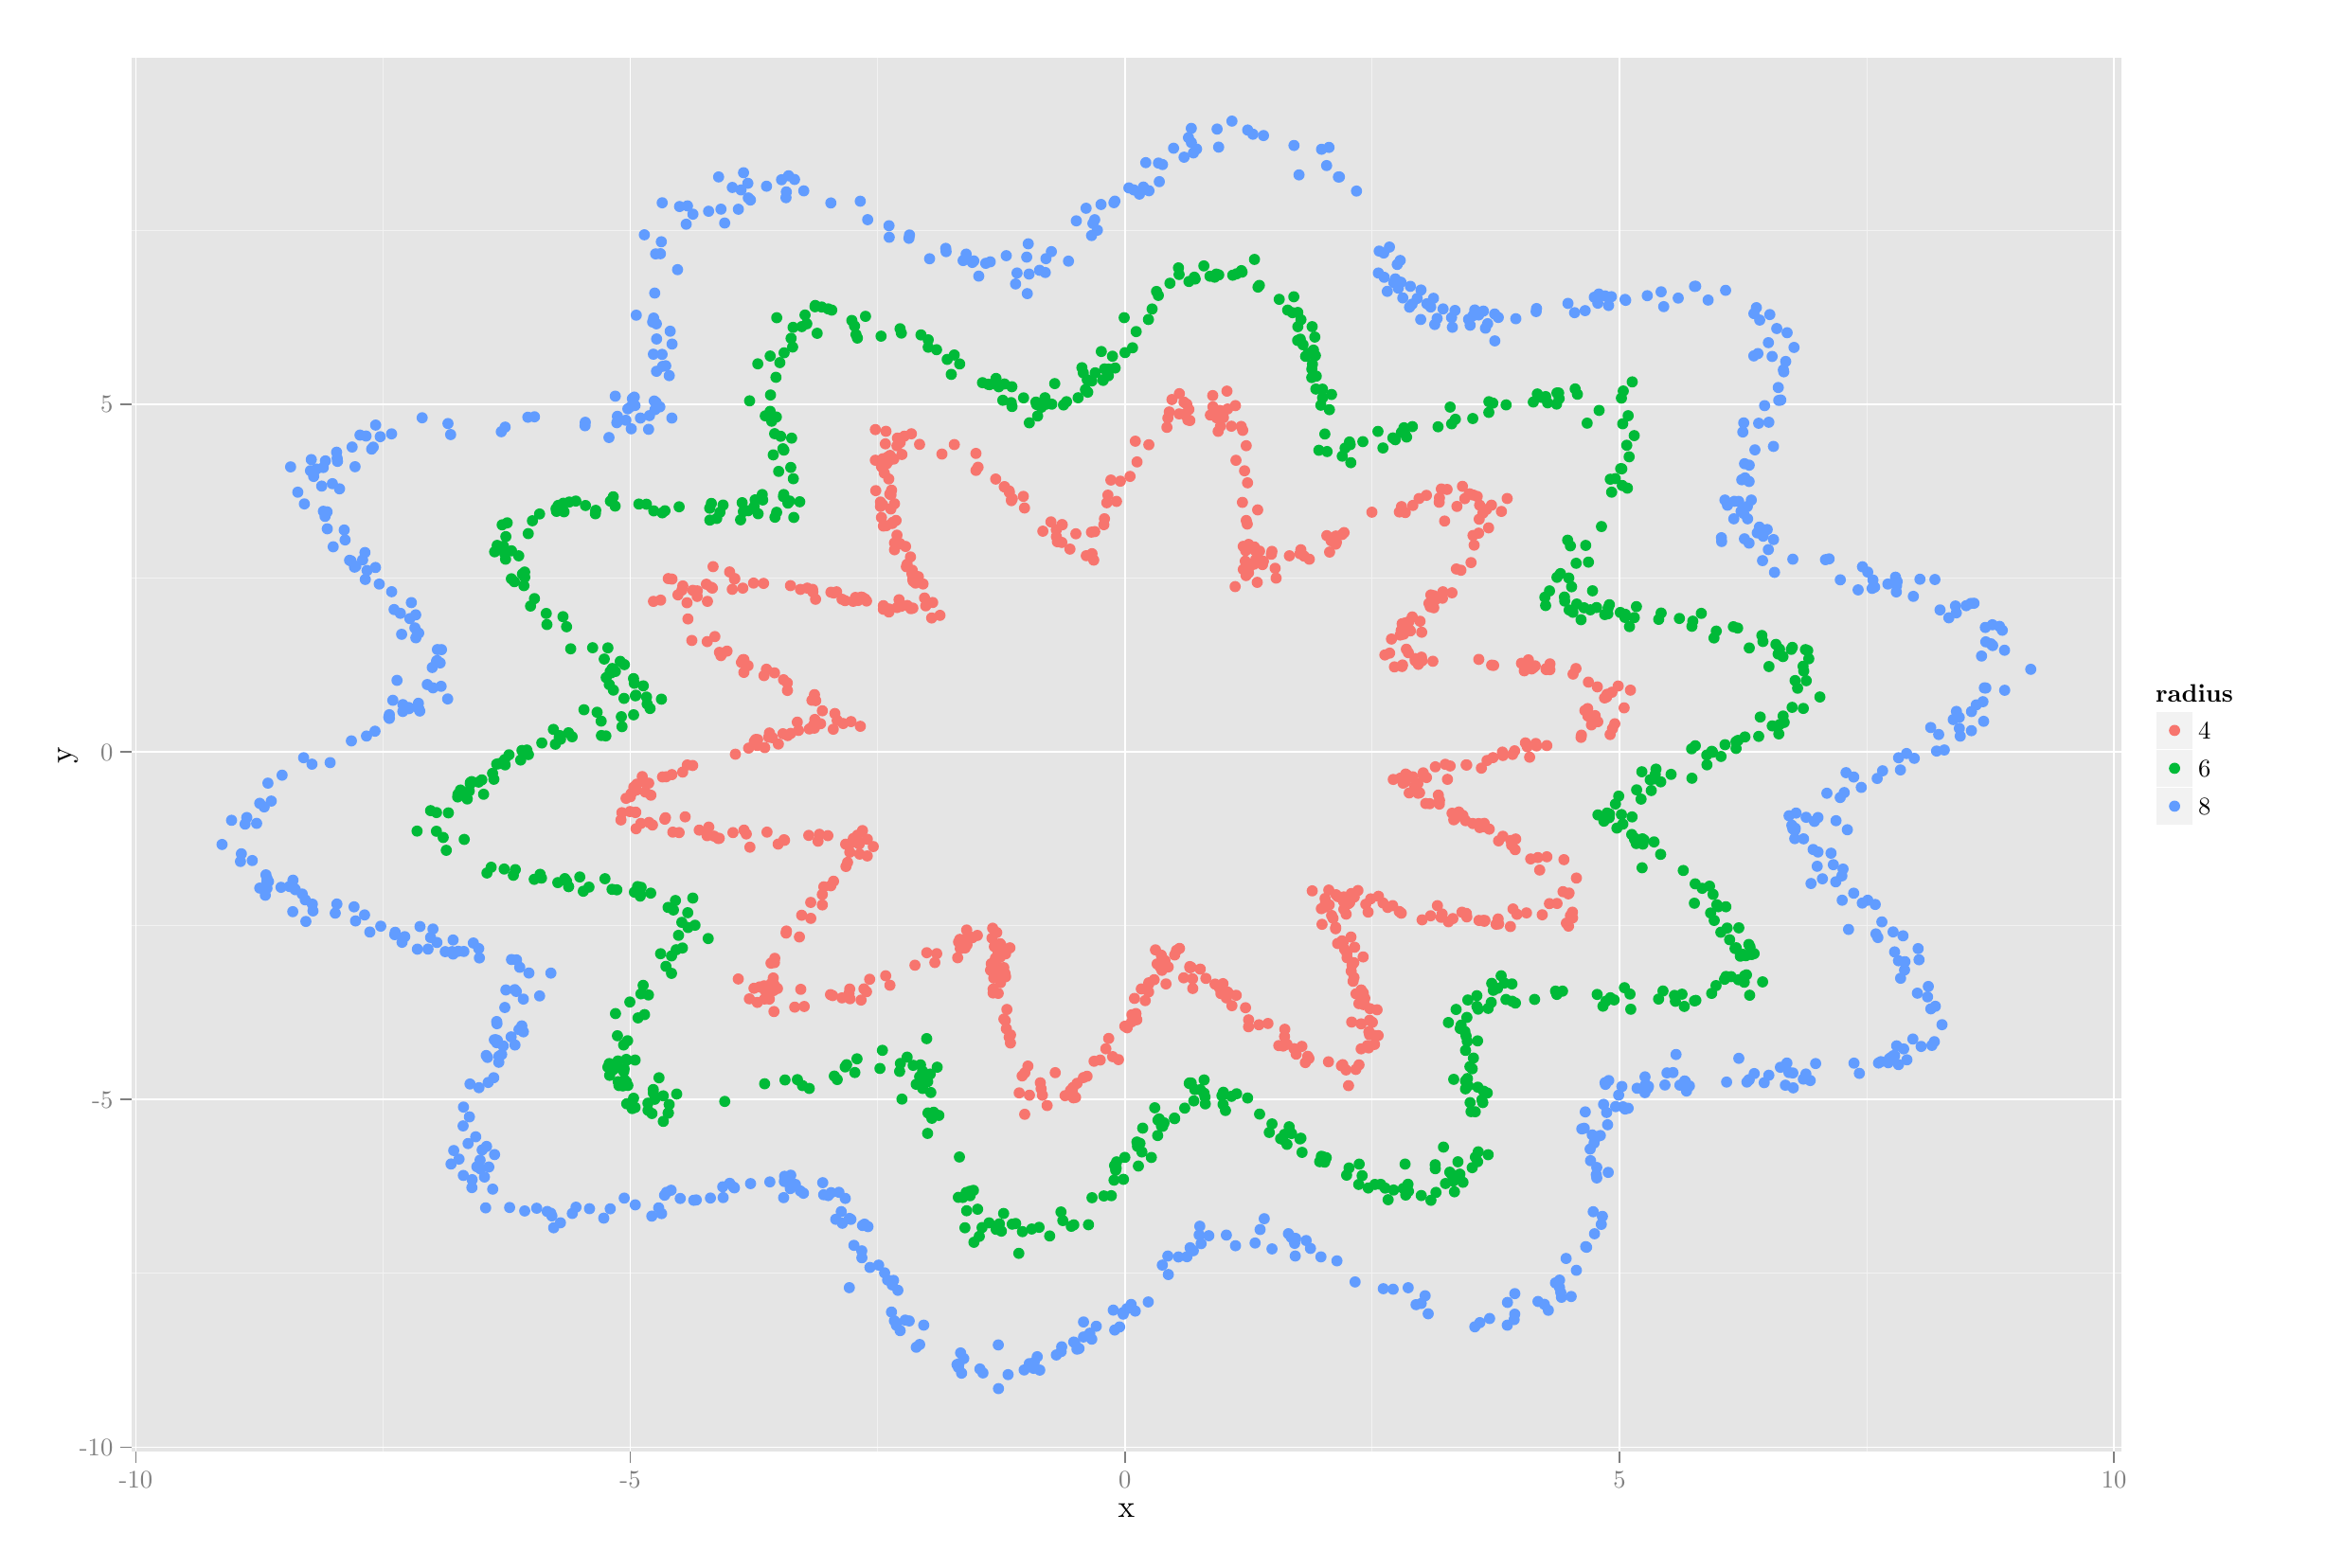
\begin{tikzpicture}[x=1pt,y=1pt]
\definecolor[named]{fillColor}{rgb}{1.00,1.00,1.00}
\path[use as bounding box,fill=fillColor,fill opacity=0.00] (0,0) rectangle (867.24,578.16);
\begin{scope}
\path[clip] (  0.00,  0.00) rectangle (867.24,578.16);
\definecolor[named]{drawColor}{rgb}{1.00,1.00,1.00}
\definecolor[named]{fillColor}{rgb}{1.00,1.00,1.00}

\path[draw=drawColor,line width= 0.6pt,line join=round,line cap=round,fill=fillColor] (  0.00, -0.00) rectangle (867.24,578.16);
\end{scope}
\begin{scope}
\path[clip] ( 40.22, 34.03) rectangle (799.33,566.12);
\definecolor[named]{fillColor}{rgb}{0.90,0.90,0.90}

\path[fill=fillColor] ( 40.22, 34.03) rectangle (799.33,566.12);
\definecolor[named]{drawColor}{rgb}{0.95,0.95,0.95}

\path[draw=drawColor,line width= 0.3pt,line join=round] ( 40.22,102.20) --
	(799.33,102.20);

\path[draw=drawColor,line width= 0.3pt,line join=round] ( 40.22,234.89) --
	(799.33,234.89);

\path[draw=drawColor,line width= 0.3pt,line join=round] ( 40.22,367.58) --
	(799.33,367.58);

\path[draw=drawColor,line width= 0.3pt,line join=round] ( 40.22,500.27) --
	(799.33,500.27);

\path[draw=drawColor,line width= 0.3pt,line join=round] (136.16, 34.03) --
	(136.16,566.12);

\path[draw=drawColor,line width= 0.3pt,line join=round] (324.85, 34.03) --
	(324.85,566.12);

\path[draw=drawColor,line width= 0.3pt,line join=round] (513.54, 34.03) --
	(513.54,566.12);

\path[draw=drawColor,line width= 0.3pt,line join=round] (702.23, 34.03) --
	(702.23,566.12);
\definecolor[named]{drawColor}{rgb}{1.00,1.00,1.00}

\path[draw=drawColor,line width= 0.6pt,line join=round] ( 40.22, 35.86) --
	(799.33, 35.86);

\path[draw=drawColor,line width= 0.6pt,line join=round] ( 40.22,168.55) --
	(799.33,168.55);

\path[draw=drawColor,line width= 0.6pt,line join=round] ( 40.22,301.24) --
	(799.33,301.24);

\path[draw=drawColor,line width= 0.6pt,line join=round] ( 40.22,433.93) --
	(799.33,433.93);

\path[draw=drawColor,line width= 0.6pt,line join=round] ( 41.81, 34.03) --
	( 41.81,566.12);

\path[draw=drawColor,line width= 0.6pt,line join=round] (230.50, 34.03) --
	(230.50,566.12);

\path[draw=drawColor,line width= 0.6pt,line join=round] (419.19, 34.03) --
	(419.19,566.12);

\path[draw=drawColor,line width= 0.6pt,line join=round] (607.88, 34.03) --
	(607.88,566.12);

\path[draw=drawColor,line width= 0.6pt,line join=round] (796.57, 34.03) --
	(796.57,566.12);
\definecolor[named]{fillColor}{rgb}{0.97,0.46,0.43}

\path[fill=fillColor] (275.63,302.64) circle (  2.13);

\path[fill=fillColor] (443.60,431.88) circle (  2.13);

\path[fill=fillColor] (476.52,371.28) circle (  2.13);

\path[fill=fillColor] (531.80,351.06) circle (  2.13);

\path[fill=fillColor] (330.41,388.37) circle (  2.13);

\path[fill=fillColor] (593.23,306.75) circle (  2.13);

\path[fill=fillColor] (506.69,245.83) circle (  2.13);

\path[fill=fillColor] (395.13,381.13) circle (  2.13);

\path[fill=fillColor] (329.60,414.35) circle (  2.13);

\path[fill=fillColor] (274.74,269.88) circle (  2.13);

\path[fill=fillColor] (368.91,209.20) circle (  2.13);

\path[fill=fillColor] (345.86,358.22) circle (  2.13);

\path[fill=fillColor] (559.63,299.03) circle (  2.13);

\path[fill=fillColor] (477.91,189.13) circle (  2.13);

\path[fill=fillColor] (345.47,352.31) circle (  2.13);

\path[fill=fillColor] (495.67,243.28) circle (  2.13);

\path[fill=fillColor] (507.38,208.89) circle (  2.13);

\path[fill=fillColor] (369.40,226.91) circle (  2.13);

\path[fill=fillColor] (526.18,392.55) circle (  2.13);

\path[fill=fillColor] (311.27,359.47) circle (  2.13);

\path[fill=fillColor] (331.02,412.97) circle (  2.13);

\path[fill=fillColor] (309.43,313.23) circle (  2.13);

\path[fill=fillColor] (256.79,271.36) circle (  2.13);

\path[fill=fillColor] (513.61,198.01) circle (  2.13);

\path[fill=fillColor] (552.13,399.23) circle (  2.13);

\path[fill=fillColor] (312.66,265.99) circle (  2.13);

\path[fill=fillColor] (324.15,400.91) circle (  2.13);

\path[fill=fillColor] (285.61,222.43) circle (  2.13);

\path[fill=fillColor] (468.47,372.86) circle (  2.13);

\path[fill=fillColor] (450.09,214.77) circle (  2.13);

\path[fill=fillColor] (329.49,399.62) circle (  2.13);

\path[fill=fillColor] (503.52,243.16) circle (  2.13);

\path[fill=fillColor] (549.63,296.21) circle (  2.13);

\path[fill=fillColor] (466.35,369.53) circle (  2.13);

\path[fill=fillColor] (373.97,195.56) circle (  2.13);

\path[fill=fillColor] (473.78,197.57) circle (  2.13);

\path[fill=fillColor] (375.33,226.43) circle (  2.13);

\path[fill=fillColor] (329.96,399.31) circle (  2.13);

\path[fill=fillColor] (532.36,337.36) circle (  2.13);

\path[fill=fillColor] (282.65,270.60) circle (  2.13);

\path[fill=fillColor] (318.00,262.21) circle (  2.13);

\path[fill=fillColor] (313.93,208.97) circle (  2.13);

\path[fill=fillColor] (285.30,202.12) circle (  2.13);

\path[fill=fillColor] (527.58,350.94) circle (  2.13);

\path[fill=fillColor] (475.29,377.74) circle (  2.13);

\path[fill=fillColor] (438.19,223.72) circle (  2.13);

\path[fill=fillColor] (536.70,335.80) circle (  2.13);

\path[fill=fillColor] (455.30,211.12) circle (  2.13);

\path[fill=fillColor] (273.83,336.43) circle (  2.13);

\path[fill=fillColor] (526.33,292.76) circle (  2.13);

\path[fill=fillColor] (338.14,369.85) circle (  2.13);

\path[fill=fillColor] (337.72,422.61) circle (  2.13);

\path[fill=fillColor] (549.65,238.24) circle (  2.13);

\path[fill=fillColor] (285.49,220.79) circle (  2.13);

\path[fill=fillColor] (535.84,238.66) circle (  2.13);

\path[fill=fillColor] (288.95,328.75) circle (  2.13);

\path[fill=fillColor] (407.43,183.15) circle (  2.13);

\path[fill=fillColor] (458.43,209.54) circle (  2.13);

\path[fill=fillColor] (373.03,199.27) circle (  2.13);

\path[fill=fillColor] (340.40,368.08) circle (  2.13);

\path[fill=fillColor] (540.23,239.35) circle (  2.13);

\path[fill=fillColor] (526.26,289.85) circle (  2.13);

\path[fill=fillColor] (286.98,304.21) circle (  2.13);

\path[fill=fillColor] (575.75,334.04) circle (  2.13);

\path[fill=fillColor] (326.80,395.51) circle (  2.13);

\path[fill=fillColor] (318.54,206.50) circle (  2.13);

\path[fill=fillColor] (375.05,192.35) circle (  2.13);

\path[fill=fillColor] (265.07,337.94) circle (  2.13);

\path[fill=fillColor] (554.37,390.02) circle (  2.13);

\path[fill=fillColor] (537.76,359.37) circle (  2.13);

\path[fill=fillColor] (603.13,323.19) circle (  2.13);

\path[fill=fillColor] (481.04,189.61) circle (  2.13);

\path[fill=fillColor] (504.43,243.26) circle (  2.13);

\path[fill=fillColor] (273.86,271.36) circle (  2.13);

\path[fill=fillColor] (508.11,248.31) circle (  2.13);

\path[fill=fillColor] (544.32,237.60) circle (  2.13);

\path[fill=fillColor] (568.09,263.90) circle (  2.13);

\path[fill=fillColor] (392.62,178.80) circle (  2.13);

\path[fill=fillColor] (329.15,354.60) circle (  2.13);

\path[fill=fillColor] (314.71,312.77) circle (  2.13);

\path[fill=fillColor] (558.21,271.73) circle (  2.13);

\path[fill=fillColor] (556.29,273.94) circle (  2.13);

\path[fill=fillColor] (529.96,335.98) circle (  2.13);

\path[fill=fillColor] (561.77,267.26) circle (  2.13);

\path[fill=fillColor] (433.32,217.84) circle (  2.13);

\path[fill=fillColor] (551.94,273.87) circle (  2.13);

\path[fill=fillColor] (430.36,214.27) circle (  2.13);

\path[fill=fillColor] (494.15,241.37) circle (  2.13);

\path[fill=fillColor] (537.15,360.80) circle (  2.13);

\path[fill=fillColor] (497.87,381.80) circle (  2.13);

\path[fill=fillColor] (254.28,296.02) circle (  2.13);

\path[fill=fillColor] (333.02,359.29) circle (  2.13);

\path[fill=fillColor] (277.52,365.63) circle (  2.13);

\path[fill=fillColor] (598.28,314.41) circle (  2.13);

\path[fill=fillColor] (501.80,181.41) circle (  2.13);

\path[fill=fillColor] (423.18,419.78) circle (  2.13);

\path[fill=fillColor] (428.33,418.43) circle (  2.13);

\path[fill=fillColor] (300.03,363.25) circle (  2.13);

\path[fill=fillColor] (332.25,356.29) circle (  2.13);

\path[fill=fillColor] (451.82,429.76) circle (  2.13);

\path[fill=fillColor] (574.39,332.87) circle (  2.13);

\path[fill=fillColor] (338.05,370.55) circle (  2.13);

\path[fill=fillColor] (404.75,177.43) circle (  2.13);

\path[fill=fillColor] (356.39,226.14) circle (  2.13);

\path[fill=fillColor] (555.21,295.01) circle (  2.13);

\path[fill=fillColor] (607.41,326.36) circle (  2.13);

\path[fill=fillColor] (398.23,378.60) circle (  2.13);

\path[fill=fillColor] (557.96,386.71) circle (  2.13);

\path[fill=fillColor] (327.41,407.62) circle (  2.13);

\path[fill=fillColor] (515.94,246.12) circle (  2.13);

\path[fill=fillColor] (499.63,234.26) circle (  2.13);

\path[fill=fillColor] (369.90,405.33) circle (  2.13);

\path[fill=fillColor] (303.74,246.78) circle (  2.13);

\path[fill=fillColor] (358.97,227.61) circle (  2.13);

\path[fill=fillColor] (238.94,273.31) circle (  2.13);

\path[fill=fillColor] (480.11,192.58) circle (  2.13);

\path[fill=fillColor] (524.92,333.80) circle (  2.13);

\path[fill=fillColor] (327.05,387.40) circle (  2.13);

\path[fill=fillColor] (315.52,358.67) circle (  2.13);

\path[fill=fillColor] (276.12,264.84) circle (  2.13);

\path[fill=fillColor] (320.62,209.70) circle (  2.13);

\path[fill=fillColor] (551.26,373.46) circle (  2.13);

\path[fill=fillColor] (469.94,374.52) circle (  2.13);

\path[fill=fillColor] (369.81,222.51) circle (  2.13);

\path[fill=fillColor] (362.36,415.12) circle (  2.13);

\path[fill=fillColor] (319.05,360.17) circle (  2.13);

\path[fill=fillColor] (455.83,208.96) circle (  2.13);

\path[fill=fillColor] (510.23,204.78) circle (  2.13);

\path[fill=fillColor] (330.16,401.09) circle (  2.13);

\path[fill=fillColor] (237.51,289.28) circle (  2.13);

\path[fill=fillColor] (338.27,367.03) circle (  2.13);

\path[fill=fillColor] (465.44,368.50) circle (  2.13);

\path[fill=fillColor] (539.47,360.21) circle (  2.13);

\path[fill=fillColor] (419.18,196.52) circle (  2.13);

\path[fill=fillColor] (283.54,206.88) circle (  2.13);

\path[fill=fillColor] (317.41,359.00) circle (  2.13);

\path[fill=fillColor] (307.69,208.20) circle (  2.13);

\path[fill=fillColor] (414.52,184.91) circle (  2.13);

\path[fill=fillColor] (561.60,237.46) circle (  2.13);

\path[fill=fillColor] (316.71,267.09) circle (  2.13);

\path[fill=fillColor] (301.24,320.77) circle (  2.13);

\path[fill=fillColor] (486.33,378.36) circle (  2.13);

\path[fill=fillColor] (354.12,418.50) circle (  2.13);

\path[fill=fillColor] (284.17,220.59) circle (  2.13);

\path[fill=fillColor] (284.22,212.78) circle (  2.13);

\path[fill=fillColor] (581.35,332.60) circle (  2.13);

\path[fill=fillColor] (560.82,235.44) circle (  2.13);

\path[fill=fillColor] (308.03,251.85) circle (  2.13);

\path[fill=fillColor] (524.65,239.67) circle (  2.13);

\path[fill=fillColor] (573.14,336.33) circle (  2.13);

\path[fill=fillColor] (588.46,234.72) circle (  2.13);

\path[fill=fillColor] (529.92,336.83) circle (  2.13);

\path[fill=fillColor] (465.49,418.06) circle (  2.13);

\path[fill=fillColor] (539.17,281.29) circle (  2.13);

\path[fill=fillColor] (290.45,324.66) circle (  2.13);

\path[fill=fillColor] (597.20,311.51) circle (  2.13);

\path[fill=fillColor] (505.45,230.56) circle (  2.13);

\path[fill=fillColor] (509.32,197.42) circle (  2.13);

\path[fill=fillColor] (368.48,230.14) circle (  2.13);

\path[fill=fillColor] (464.04,396.43) circle (  2.13);

\path[fill=fillColor] (563.42,269.02) circle (  2.13);

\path[fill=fillColor] (253.96,343.74) circle (  2.13);

\path[fill=fillColor] (327.80,418.77) circle (  2.13);

\path[fill=fillColor] (371.61,228.01) circle (  2.13);

\path[fill=fillColor] (542.64,236.37) circle (  2.13);

\path[fill=fillColor] (503.89,224.35) circle (  2.13);

\path[fill=fillColor] (268.38,369.88) circle (  2.13);

\path[fill=fillColor] (285.51,331.37) circle (  2.13);

\path[fill=fillColor] (395.29,387.90) circle (  2.13);

\path[fill=fillColor] (375.56,193.22) circle (  2.13);

\path[fill=fillColor] (496.87,182.95) circle (  2.13);

\path[fill=fillColor] (468.57,379.42) circle (  2.13);

\path[fill=fillColor] (508.48,205.15) circle (  2.13);

\path[fill=fillColor] (273.42,363.71) circle (  2.13);

\path[fill=fillColor] (284.72,210.15) circle (  2.13);

\path[fill=fillColor] (594.70,316.99) circle (  2.13);

\path[fill=fillColor] (568.79,239.23) circle (  2.13);

\path[fill=fillColor] (308.13,361.85) circle (  2.13);

\path[fill=fillColor] (281.50,330.32) circle (  2.13);

\path[fill=fillColor] (347.40,224.22) circle (  2.13);

\path[fill=fillColor] (319.63,210.77) circle (  2.13);

\path[fill=fillColor] (252.12,358.12) circle (  2.13);

\path[fill=fillColor] (300.76,323.07) circle (  2.13);

\path[fill=fillColor] (499.59,233.72) circle (  2.13);

\path[fill=fillColor] (573.62,299.18) circle (  2.13);

\path[fill=fillColor] (454.78,423.54) circle (  2.13);

\path[fill=fillColor] (605.24,310.09) circle (  2.13);

\path[fill=fillColor] (380.45,398.72) circle (  2.13);

\path[fill=fillColor] (294.20,312.56) circle (  2.13);

\path[fill=fillColor] (333.80,356.76) circle (  2.13);

\path[fill=fillColor] (443.96,219.28) circle (  2.13);

\path[fill=fillColor] (541.18,389.31) circle (  2.13);

\path[fill=fillColor] (549.20,274.94) circle (  2.13);

\path[fill=fillColor] (368.91,210.67) circle (  2.13);

\path[fill=fillColor] (279.06,305.91) circle (  2.13);

\path[fill=fillColor] (438.89,225.45) circle (  2.13);

\path[fill=fillColor] (291.60,364.66) circle (  2.13);

\path[fill=fillColor] (506.85,226.67) circle (  2.13);

\path[fill=fillColor] (250.47,293.51) circle (  2.13);

\path[fill=fillColor] (456.26,429.51) circle (  2.13);

\path[fill=fillColor] (330.60,388.80) circle (  2.13);

\path[fill=fillColor] (463.56,425.41) circle (  2.13);

\path[fill=fillColor] (441.97,430.05) circle (  2.13);

\path[fill=fillColor] (466.41,380.40) circle (  2.13);

\path[fill=fillColor] (395.17,387.91) circle (  2.13);

\path[fill=fillColor] (525.64,349.57) circle (  2.13);

\path[fill=fillColor] (252.24,296.21) circle (  2.13);

\path[fill=fillColor] (298.02,363.71) circle (  2.13);

\path[fill=fillColor] (283.57,308.44) circle (  2.13);

\path[fill=fillColor] (260.44,272.52) circle (  2.13);

\path[fill=fillColor] (371.56,222.82) circle (  2.13);

\path[fill=fillColor] (230.51,284.11) circle (  2.13);

\path[fill=fillColor] (235.04,291.80) circle (  2.13);

\path[fill=fillColor] (319.07,271.19) circle (  2.13);

\path[fill=fillColor] (554.54,395.36) circle (  2.13);

\path[fill=fillColor] (455.37,431.54) circle (  2.13);

\path[fill=fillColor] (421.86,200.92) circle (  2.13);

\path[fill=fillColor] (540.53,362.30) circle (  2.13);

\path[fill=fillColor] (506.25,213.67) circle (  2.13);

\path[fill=fillColor] (505.54,217.54) circle (  2.13);

\path[fill=fillColor] (314.32,207.01) circle (  2.13);

\path[fill=fillColor] (262.42,269.07) circle (  2.13);

\path[fill=fillColor] (546.61,278.28) circle (  2.13);

\path[fill=fillColor] (278.89,303.66) circle (  2.13);

\path[fill=fillColor] (387.23,172.66) circle (  2.13);

\path[fill=fillColor] (417.47,404.52) circle (  2.13);

\path[fill=fillColor] (425.46,210.76) circle (  2.13);

\path[fill=fillColor] (282.43,332.76) circle (  2.13);

\path[fill=fillColor] (498.07,238.78) circle (  2.13);

\path[fill=fillColor] (326.29,410.20) circle (  2.13);

\path[fill=fillColor] (435.23,425.07) circle (  2.13);

\path[fill=fillColor] (270.23,367.19) circle (  2.13);

\path[fill=fillColor] (584.07,243.37) circle (  2.13);

\path[fill=fillColor] (358.83,233.23) circle (  2.13);

\path[fill=fillColor] (442.81,433.88) circle (  2.13);

\path[fill=fillColor] (232.56,278.21) circle (  2.13);

\path[fill=fillColor] (312.43,358.93) circle (  2.13);

\path[fill=fillColor] (295.87,238.87) circle (  2.13);

\path[fill=fillColor] (311.26,207.34) circle (  2.13);

\path[fill=fillColor] (500.47,245.96) circle (  2.13);

\path[fill=fillColor] (531.63,285.61) circle (  2.13);

\path[fill=fillColor] (390.98,388.99) circle (  2.13);

\path[fill=fillColor] (403.38,176.92) circle (  2.13);

\path[fill=fillColor] (327.02,355.66) circle (  2.13);

\path[fill=fillColor] (535.70,356.60) circle (  2.13);

\path[fill=fillColor] (526.60,291.89) circle (  2.13);

\path[fill=fillColor] (407.69,385.28) circle (  2.13);

\path[fill=fillColor] (428.30,213.09) circle (  2.13);

\path[fill=fillColor] (522.03,333.65) circle (  2.13);

\path[fill=fillColor] (407.31,374.39) circle (  2.13);

\path[fill=fillColor] (375.90,397.10) circle (  2.13);

\path[fill=fillColor] (325.94,394.88) circle (  2.13);

\path[fill=fillColor] (524.73,394.82) circle (  2.13);

\path[fill=fillColor] (452.70,437.19) circle (  2.13);

\path[fill=fillColor] (532.56,335.95) circle (  2.13);

\path[fill=fillColor] (230.77,285.26) circle (  2.13);

\path[fill=fillColor] (262.75,345.22) circle (  2.13);

\path[fill=fillColor] (339.09,219.81) circle (  2.13);

\path[fill=fillColor] (355.39,222.65) circle (  2.13);

\path[fill=fillColor] (464.16,423.93) circle (  2.13);

\path[fill=fillColor] (382.78,170.19) circle (  2.13);

\path[fill=fillColor] (567.27,241.26) circle (  2.13);

\path[fill=fillColor] (581.18,243.31) circle (  2.13);

\path[fill=fillColor] (562.86,392.98) circle (  2.13);

\path[fill=fillColor] (460.03,204.36) circle (  2.13);

\path[fill=fillColor] (471.71,372.69) circle (  2.13);

\path[fill=fillColor] (521.35,242.56) circle (  2.13);

\path[fill=fillColor] (504.96,243.70) circle (  2.13);

\path[fill=fillColor] (475.07,376.64) circle (  2.13);

\path[fill=fillColor] (514.44,189.59) circle (  2.13);

\path[fill=fillColor] (511.99,240.08) circle (  2.13);

\path[fill=fillColor] (433.07,223.64) circle (  2.13);

\path[fill=fillColor] (284.69,306.64) circle (  2.13);

\path[fill=fillColor] (554.58,272.33) circle (  2.13);

\path[fill=fillColor] (572.73,303.17) circle (  2.13);

\path[fill=fillColor] (273.82,331.55) circle (  2.13);

\path[fill=fillColor] (327.93,215.77) circle (  2.13);

\path[fill=fillColor] (261.37,364.03) circle (  2.13);

\path[fill=fillColor] (542.27,290.74) circle (  2.13);

\path[fill=fillColor] (497.15,242.83) circle (  2.13);

\path[fill=fillColor] (572.02,304.64) circle (  2.13);

\path[fill=fillColor] (300.14,362.26) circle (  2.13);

\path[fill=fillColor] (561.80,235.56) circle (  2.13);

\path[fill=fillColor] (270.35,367.35) circle (  2.13);

\path[fill=fillColor] (461.57,412.49) circle (  2.13);

\path[fill=fillColor] (559.89,334.22) circle (  2.13);

\path[fill=fillColor] (580.18,303.63) circle (  2.13);

\path[fill=fillColor] (443.22,427.90) circle (  2.13);

\path[fill=fillColor] (455.89,211.56) circle (  2.13);

\path[fill=fillColor] (556.32,236.56) circle (  2.13);

\path[fill=fillColor] (484.55,185.87) circle (  2.13);

\path[fill=fillColor] (544.67,275.28) circle (  2.13);

\path[fill=fillColor] (340.85,418.57) circle (  2.13);

\path[fill=fillColor] (232.69,271.89) circle (  2.13);

\path[fill=fillColor] (387.89,385.44) circle (  2.13);

\path[fill=fillColor] (358.21,226.37) circle (  2.13);

\path[fill=fillColor] (264.42,268.23) circle (  2.13);

\path[fill=fillColor] (242.78,291.66) circle (  2.13);

\path[fill=fillColor] (318.26,310.98) circle (  2.13);

\path[fill=fillColor] (578.43,239.04) circle (  2.13);

\path[fill=fillColor] (495.55,242.01) circle (  2.13);

\path[fill=fillColor] (524.97,350.12) circle (  2.13);

\path[fill=fillColor] (285.18,210.15) circle (  2.13);

\path[fill=fillColor] (246.39,367.16) circle (  2.13);

\path[fill=fillColor] (567.11,300.25) circle (  2.13);

\path[fill=fillColor] (524.62,347.59) circle (  2.13);

\path[fill=fillColor] (426.95,206.29) circle (  2.13);

\path[fill=fillColor] (570.51,335.03) circle (  2.13);

\path[fill=fillColor] (370.65,217.79) circle (  2.13);

\path[fill=fillColor] (529.68,286.85) circle (  2.13);

\path[fill=fillColor] (598.62,315.04) circle (  2.13);

\path[fill=fillColor] (455.67,425.49) circle (  2.13);

\path[fill=fillColor] (300.89,313.59) circle (  2.13);

\path[fill=fillColor] (512.54,198.80) circle (  2.13);

\path[fill=fillColor] (515.82,192.97) circle (  2.13);

\path[fill=fillColor] (399.27,170.83) circle (  2.13);

\path[fill=fillColor] (271.69,214.55) circle (  2.13);

\path[fill=fillColor] (605.01,323.98) circle (  2.13);

\path[fill=fillColor] (531.16,334.62) circle (  2.13);

\path[fill=fillColor] (452.79,432.89) circle (  2.13);

\path[fill=fillColor] (304.33,249.72) circle (  2.13);

\path[fill=fillColor] (575.98,304.43) circle (  2.13);

\path[fill=fillColor] (453.58,212.60) circle (  2.13);

\path[fill=fillColor] (303.76,242.81) circle (  2.13);

\path[fill=fillColor] (466.83,371.98) circle (  2.13);

\path[fill=fillColor] (528.83,352.72) circle (  2.13);

\path[fill=fillColor] (278.34,305.95) circle (  2.13);

\path[fill=fillColor] (502.31,181.87) circle (  2.13);

\path[fill=fillColor] (423.74,199.00) circle (  2.13);

\path[fill=fillColor] (332.42,420.96) circle (  2.13);

\path[fill=fillColor] (439.91,430.20) circle (  2.13);

\path[fill=fillColor] (440.03,226.21) circle (  2.13);

\path[fill=fillColor] (306.87,208.59) circle (  2.13);

\path[fill=fillColor] (556.62,272.58) circle (  2.13);

\path[fill=fillColor] (539.11,396.49) circle (  2.13);

\path[fill=fillColor] (563.23,301.13) circle (  2.13);

\path[fill=fillColor] (250.17,362.93) circle (  2.13);

\path[fill=fillColor] (456.47,430.11) circle (  2.13);

\path[fill=fillColor] (328.25,411.15) circle (  2.13);

\path[fill=fillColor] (393.43,381.41) circle (  2.13);

\path[fill=fillColor] (333.45,419.25) circle (  2.13);

\path[fill=fillColor] (575.23,333.48) circle (  2.13);

\path[fill=fillColor] (323.19,265.08) circle (  2.13);

\path[fill=fillColor] (328.04,423.56) circle (  2.13);

\path[fill=fillColor] (526.59,340.39) circle (  2.13);

\path[fill=fillColor] (317.82,266.02) circle (  2.13);

\path[fill=fillColor] (295.53,210.60) circle (  2.13);

\path[fill=fillColor] (259.83,343.30) circle (  2.13);

\path[fill=fillColor] (445.08,210.92) circle (  2.13);

\path[fill=fillColor] (539.24,282.72) circle (  2.13);

\path[fill=fillColor] (312.77,257.49) circle (  2.13);

\path[fill=fillColor] (399.38,173.12) circle (  2.13);

\path[fill=fillColor] (244.97,367.35) circle (  2.13);

\path[fill=fillColor] (290.54,307.43) circle (  2.13);

\path[fill=fillColor] (599.62,312.73) circle (  2.13);

\path[fill=fillColor] (444.41,219.04) circle (  2.13);

\path[fill=fillColor] (505.57,247.15) circle (  2.13);

\path[fill=fillColor] (323.99,424.21) circle (  2.13);

\path[fill=fillColor] (497.30,377.47) circle (  2.13);

\path[fill=fillColor] (320.63,358.80) circle (  2.13);

\path[fill=fillColor] (302.64,269.76) circle (  2.13);

\path[fill=fillColor] (512.33,194.21) circle (  2.13);

\path[fill=fillColor] (318.59,360.29) circle (  2.13);

\path[fill=fillColor] (554.22,336.51) circle (  2.13);

\path[fill=fillColor] (444.01,218.83) circle (  2.13);

\path[fill=fillColor] (373.29,402.39) circle (  2.13);

\path[fill=fillColor] (534.24,399.12) circle (  2.13);

\path[fill=fillColor] (502.04,229.09) circle (  2.13);

\path[fill=fillColor] (456.61,212.77) circle (  2.13);

\path[fill=fillColor] (550.49,399.58) circle (  2.13);

\path[fill=fillColor] (506.53,220.76) circle (  2.13);

\path[fill=fillColor] (489.56,374.74) circle (  2.13);

\path[fill=fillColor] (302.11,267.14) circle (  2.13);

\path[fill=fillColor] (411.17,387.92) circle (  2.13);

\path[fill=fillColor] (359.35,231.17) circle (  2.13);

\path[fill=fillColor] (289.33,267.45) circle (  2.13);

\path[fill=fillColor] (291.68,308.27) circle (  2.13);

\path[fill=fillColor] (289.93,232.08) circle (  2.13);

\path[fill=fillColor] (370.01,221.49) circle (  2.13);

\path[fill=fillColor] (510.39,205.21) circle (  2.13);

\path[fill=fillColor] (521.59,290.70) circle (  2.13);

\path[fill=fillColor] (537.64,295.52) circle (  2.13);

\path[fill=fillColor] (513.44,392.69) circle (  2.13);

\path[fill=fillColor] (512.33,194.47) circle (  2.13);

\path[fill=fillColor] (612.09,324.77) circle (  2.13);

\path[fill=fillColor] (314.20,210.71) circle (  2.13);

\path[fill=fillColor] (404.47,376.08) circle (  2.13);

\path[fill=fillColor] (236.25,285.90) circle (  2.13);

\path[fill=fillColor] (288.72,308.13) circle (  2.13);

\path[fill=fillColor] (518.39,338.20) circle (  2.13);

\path[fill=fillColor] (281.33,365.52) circle (  2.13);

\path[fill=fillColor] (434.49,221.53) circle (  2.13);

\path[fill=fillColor] (422.85,207.14) circle (  2.13);

\path[fill=fillColor] (286.90,266.03) circle (  2.13);

\path[fill=fillColor] (326.83,413.09) circle (  2.13);

\path[fill=fillColor] (586.70,260.08) circle (  2.13);

\path[fill=fillColor] (285.03,214.92) circle (  2.13);

\path[fill=fillColor] (421.80,198.21) circle (  2.13);

\path[fill=fillColor] (242.07,359.13) circle (  2.13);

\path[fill=fillColor] (348.64,353.32) circle (  2.13);

\path[fill=fillColor] (456.28,209.61) circle (  2.13);

\path[fill=fillColor] (368.74,233.92) circle (  2.13);

\path[fill=fillColor] (337.55,355.86) circle (  2.13);

\path[fill=fillColor] (502.73,241.13) circle (  2.13);

\path[fill=fillColor] (376.00,397.72) circle (  2.13);

\path[fill=fillColor] (436.12,430.94) circle (  2.13);

\path[fill=fillColor] (539.21,398.15) circle (  2.13);

\path[fill=fillColor] (543.28,295.83) circle (  2.13);

\path[fill=fillColor] (428.25,209.60) circle (  2.13);

\path[fill=fillColor] (332.22,418.01) circle (  2.13);

\path[fill=fillColor] (281.70,206.91) circle (  2.13);

\path[fill=fillColor] (472.04,373.96) circle (  2.13);

\path[fill=fillColor] (421.16,406.35) circle (  2.13);

\path[fill=fillColor] (517.68,243.57) circle (  2.13);

\path[fill=fillColor] (329.10,405.37) circle (  2.13);

\path[fill=fillColor] (527.67,285.56) circle (  2.13);

\path[fill=fillColor] (329.20,355.77) circle (  2.13);

\path[fill=fillColor] (296.85,204.05) circle (  2.13);

\path[fill=fillColor] (278.97,205.61) circle (  2.13);

\path[fill=fillColor] (373.69,215.41) circle (  2.13);

\path[fill=fillColor] (489.41,184.21) circle (  2.13);

\path[fill=fillColor] (539.93,401.55) circle (  2.13);

\path[fill=fillColor] (375.53,190.11) circle (  2.13);

\path[fill=fillColor] (264.00,268.16) circle (  2.13);

\path[fill=fillColor] (495.90,242.91) circle (  2.13);

\path[fill=fillColor] (515.41,202.80) circle (  2.13);

\path[fill=fillColor] (342.18,365.29) circle (  2.13);

\path[fill=fillColor] (285.39,212.27) circle (  2.13);

\path[fill=fillColor] (371.98,227.36) circle (  2.13);

\path[fill=fillColor] (571.57,332.14) circle (  2.13);

\path[fill=fillColor] (299.79,320.91) circle (  2.13);

\path[fill=fillColor] (576.25,303.49) circle (  2.13);

\path[fill=fillColor] (557.37,297.94) circle (  2.13);

\path[fill=fillColor] (554.15,384.69) circle (  2.13);

\path[fill=fillColor] (275.41,334.11) circle (  2.13);

\path[fill=fillColor] (430.86,225.66) circle (  2.13);

\path[fill=fillColor] (362.90,231.17) circle (  2.13);

\path[fill=fillColor] (506.60,215.12) circle (  2.13);

\path[fill=fillColor] (337.95,369.16) circle (  2.13);

\path[fill=fillColor] (447.95,218.31) circle (  2.13);

\path[fill=fillColor] (376.24,397.80) circle (  2.13);

\path[fill=fillColor] (512.54,193.25) circle (  2.13);

\path[fill=fillColor] (588.66,247.35) circle (  2.13);

\path[fill=fillColor] (507.30,180.03) circle (  2.13);

\path[fill=fillColor] (596.05,327.84) circle (  2.13);

\path[fill=fillColor] (441.63,214.99) circle (  2.13);

\path[fill=fillColor] (374.17,202.92) circle (  2.13);

\path[fill=fillColor] (299.35,237.68) circle (  2.13);

\path[fill=fillColor] (589.94,240.04) circle (  2.13);

\path[fill=fillColor] (466.38,196.32) circle (  2.13);

\path[fill=fillColor] (532.58,237.11) circle (  2.13);

\path[fill=fillColor] (544.02,277.80) circle (  2.13);

\path[fill=fillColor] (445.00,214.63) circle (  2.13);

\path[fill=fillColor] (543.99,361.93) circle (  2.13);

\path[fill=fillColor] (500.36,228.09) circle (  2.13);

\path[fill=fillColor] (435.59,428.61) circle (  2.13);

\path[fill=fillColor] (298.81,309.96) circle (  2.13);

\path[fill=fillColor] (307.03,362.15) circle (  2.13);

\path[fill=fillColor] (331.29,380.96) circle (  2.13);

\path[fill=fillColor] (387.72,170.20) circle (  2.13);

\path[fill=fillColor] (465.88,388.16) circle (  2.13);

\path[fill=fillColor] (548.16,276.96) circle (  2.13);

\path[fill=fillColor] (293.22,203.80) circle (  2.13);

\path[fill=fillColor] (412.72,399.19) circle (  2.13);

\path[fill=fillColor] (261.80,363.72) circle (  2.13);

\path[fill=fillColor] (441.74,434.69) circle (  2.13);

\path[fill=fillColor] (389.52,166.25) circle (  2.13);

\path[fill=fillColor] (524.27,291.17) circle (  2.13);

\path[fill=fillColor] (380.90,394.29) circle (  2.13);

\path[fill=fillColor] (469.45,374.07) circle (  2.13);

\path[fill=fillColor] (527.04,292.18) circle (  2.13);

\path[fill=fillColor] (480.21,195.35) circle (  2.13);

\path[fill=fillColor] (531.43,397.91) circle (  2.13);

\path[fill=fillColor] (380.97,162.91) circle (  2.13);

\path[fill=fillColor] (566.74,265.60) circle (  2.13);

\path[fill=fillColor] (602.99,322.17) circle (  2.13);

\path[fill=fillColor] (469.86,393.57) circle (  2.13);

\path[fill=fillColor] (599.45,326.02) circle (  2.13);

\path[fill=fillColor] (479.56,188.95) circle (  2.13);

\path[fill=fillColor] (303.07,311.96) circle (  2.13);

\path[fill=fillColor] (523.91,392.77) circle (  2.13);

\path[fill=fillColor] (334.12,414.71) circle (  2.13);

\path[fill=fillColor] (428.22,212.50) circle (  2.13);

\path[fill=fillColor] (539.85,238.07) circle (  2.13);

\path[fill=fillColor] (256.01,360.54) circle (  2.13);

\path[fill=fillColor] (527.34,339.08) circle (  2.13);

\path[fill=fillColor] (326.24,395.56) circle (  2.13);

\path[fill=fillColor] (537.04,356.21) circle (  2.13);

\path[fill=fillColor] (535.93,361.11) circle (  2.13);

\path[fill=fillColor] (294.66,309.41) circle (  2.13);

\path[fill=fillColor] (465.99,403.90) circle (  2.13);

\path[fill=fillColor] (305.86,269.25) circle (  2.13);

\path[fill=fillColor] (586.35,247.87) circle (  2.13);

\path[fill=fillColor] (336.18,357.08) circle (  2.13);

\path[fill=fillColor] (416.74,183.77) circle (  2.13);

\path[fill=fillColor] (338.30,356.08) circle (  2.13);

\path[fill=fillColor] (393.03,385.94) circle (  2.13);

\path[fill=fillColor] (252.47,351.95) circle (  2.13);

\path[fill=fillColor] (606.11,311.95) circle (  2.13);

\path[fill=fillColor] (555.95,236.90) circle (  2.13);

\path[fill=fillColor] (511.68,189.09) circle (  2.13);

\path[fill=fillColor] (498.60,237.72) circle (  2.13);

\path[fill=fillColor] (567.89,301.61) circle (  2.13);

\path[fill=fillColor] (466.39,198.95) circle (  2.13);

\path[fill=fillColor] (547.41,370.53) circle (  2.13);

\path[fill=fillColor] (434.88,212.66) circle (  2.13);

\path[fill=fillColor] (524.22,345.80) circle (  2.13);

\path[fill=fillColor] (487.57,375.93) circle (  2.13);

\path[fill=fillColor] (512.68,203.23) circle (  2.13);

\path[fill=fillColor] (486.73,188.83) circle (  2.13);

\path[fill=fillColor] (503.97,222.66) circle (  2.13);

\path[fill=fillColor] (327.03,357.01) circle (  2.13);

\path[fill=fillColor] (470.57,377.82) circle (  2.13);

\path[fill=fillColor] (290.38,327.54) circle (  2.13);

\path[fill=fillColor] (579.95,332.62) circle (  2.13);

\path[fill=fillColor] (336.11,372.82) circle (  2.13);

\path[fill=fillColor] (559.13,334.32) circle (  2.13);

\path[fill=fillColor] (382.19,181.31) circle (  2.13);

\path[fill=fillColor] (534.26,291.42) circle (  2.13);

\path[fill=fillColor] (510.09,222.96) circle (  2.13);

\path[fill=fillColor] (326.59,409.76) circle (  2.13);

\path[fill=fillColor] (423.83,411.87) circle (  2.13);

\path[fill=fillColor] (373.56,198.66) circle (  2.13);

\path[fill=fillColor] (465.50,389.51) circle (  2.13);

\path[fill=fillColor] (581.38,334.80) circle (  2.13);

\path[fill=fillColor] (411.40,390.17) circle (  2.13);

\path[fill=fillColor] (360.96,230.27) circle (  2.13);

\path[fill=fillColor] (331.89,389.53) circle (  2.13);

\path[fill=fillColor] (411.93,187.91) circle (  2.13);

\path[fill=fillColor] (393.06,383.35) circle (  2.13);

\path[fill=fillColor] (232.45,278.08) circle (  2.13);

\path[fill=fillColor] (277.82,305.24) circle (  2.13);

\path[fill=fillColor] (227.28,278.01) circle (  2.13);

\path[fill=fillColor] (277.68,211.00) circle (  2.13);

\path[fill=fillColor] (499.63,380.51) circle (  2.13);

\path[fill=fillColor] (321.81,214.44) circle (  2.13);

\path[fill=fillColor] (300.52,311.66) circle (  2.13);

\path[fill=fillColor] (591.47,253.06) circle (  2.13);

\path[fill=fillColor] (469.69,365.91) circle (  2.13);

\path[fill=fillColor] (490.67,248.18) circle (  2.13);

\path[fill=fillColor] (289.14,267.68) circle (  2.13);

\path[fill=fillColor] (465.52,371.09) circle (  2.13);

\path[fill=fillColor] (508.52,181.78) circle (  2.13);

\path[fill=fillColor] (295.41,363.22) circle (  2.13);

\path[fill=fillColor] (320.90,261.50) circle (  2.13);

\path[fill=fillColor] (272.89,335.37) circle (  2.13);

\path[fill=fillColor] (496.24,383.74) circle (  2.13);

\path[fill=fillColor] (456.32,431.18) circle (  2.13);

\path[fill=fillColor] (409.77,183.61) circle (  2.13);

\path[fill=fillColor] (553.62,398.70) circle (  2.13);

\path[fill=fillColor] (339.29,365.64) circle (  2.13);

\path[fill=fillColor] (483.74,187.95) circle (  2.13);

\path[fill=fillColor] (300.73,310.27) circle (  2.13);

\path[fill=fillColor] (299.33,243.77) circle (  2.13);

\path[fill=fillColor] (465.11,374.00) circle (  2.13);

\path[fill=fillColor] (375.02,400.80) circle (  2.13);

\path[fill=fillColor] (267.39,339.67) circle (  2.13);

\path[fill=fillColor] (331.28,395.92) circle (  2.13);

\path[fill=fillColor] (555.79,392.34) circle (  2.13);

\path[fill=fillColor] (239.32,358.65) circle (  2.13);

\path[fill=fillColor] (469.12,374.63) circle (  2.13);

\path[fill=fillColor] (556.57,236.87) circle (  2.13);

\path[fill=fillColor] (519.46,241.85) circle (  2.13);

\path[fill=fillColor] (552.45,380.11) circle (  2.13);

\path[fill=fillColor] (228.87,283.48) circle (  2.13);

\path[fill=fillColor] (262.07,371.91) circle (  2.13);

\path[fill=fillColor] (499.72,383.60) circle (  2.13);

\path[fill=fillColor] (371.61,217.09) circle (  2.13);

\path[fill=fillColor] (461.26,364.29) circle (  2.13);

\path[fill=fillColor] (372.99,218.88) circle (  2.13);

\path[fill=fillColor] (566.48,267.38) circle (  2.13);

\path[fill=fillColor] (502.47,228.57) circle (  2.13);

\path[fill=fillColor] (234.51,273.91) circle (  2.13);

\path[fill=fillColor] (580.20,261.18) circle (  2.13);

\path[fill=fillColor] (559.06,395.37) circle (  2.13);

\path[fill=fillColor] (550.74,399.70) circle (  2.13);

\path[fill=fillColor] (505.73,198.11) circle (  2.13);

\path[fill=fillColor] (502.09,384.19) circle (  2.13);

\path[fill=fillColor] (511.10,243.06) circle (  2.13);

\path[fill=fillColor] (459.81,425.50) circle (  2.13);

\path[fill=fillColor] (458.38,432.06) circle (  2.13);

\path[fill=fillColor] (373.68,224.14) circle (  2.13);

\path[fill=fillColor] (315.10,266.59) circle (  2.13);

\path[fill=fillColor] (315.57,268.15) circle (  2.13);

\path[fill=fillColor] (590.00,237.84) circle (  2.13);

\path[fill=fillColor] (343.21,356.95) circle (  2.13);

\path[fill=fillColor] (535.50,281.44) circle (  2.13);

\path[fill=fillColor] (563.44,299.83) circle (  2.13);

\path[fill=fillColor] (386.92,174.94) circle (  2.13);

\path[fill=fillColor] (545.66,371.01) circle (  2.13);

\path[fill=fillColor] (538.44,242.53) circle (  2.13);

\path[fill=fillColor] (485.99,376.85) circle (  2.13);

\path[fill=fillColor] (246.71,270.59) circle (  2.13);

\path[fill=fillColor] (244.12,291.71) circle (  2.13);

\path[fill=fillColor] (270.58,300.33) circle (  2.13);

\path[fill=fillColor] (277.86,304.21) circle (  2.13);

\path[fill=fillColor] (329.90,393.91) circle (  2.13);

\path[fill=fillColor] (496.99,248.48) circle (  2.13);

\path[fill=fillColor] (328.14,387.53) circle (  2.13);

\path[fill=fillColor] (465.27,378.02) circle (  2.13);

\path[fill=fillColor] (281.56,211.94) circle (  2.13);

\path[fill=fillColor] (465.21,203.58) circle (  2.13);

\path[fill=fillColor] (295.01,230.58) circle (  2.13);

\path[fill=fillColor] (301.17,359.45) circle (  2.13);

\path[fill=fillColor] (299.77,310.56) circle (  2.13);

\path[fill=fillColor] (468.79,378.15) circle (  2.13);

\path[fill=fillColor] (337.39,375.61) circle (  2.13);

\path[fill=fillColor] (461.37,433.36) circle (  2.13);

\path[fill=fillColor] (587.64,235.86) circle (  2.13);

\path[fill=fillColor] (557.17,393.75) circle (  2.13);

\path[fill=fillColor] (232.75,286.61) circle (  2.13);

\path[fill=fillColor] (527.73,347.79) circle (  2.13);

\path[fill=fillColor] (520.90,344.27) circle (  2.13);

\path[fill=fillColor] (349.39,414.87) circle (  2.13);

\path[fill=fillColor] (338.43,366.33) circle (  2.13);

\path[fill=fillColor] (456.80,428.78) circle (  2.13);

\path[fill=fillColor] (259.51,365.21) circle (  2.13);

\path[fill=fillColor] (251.41,276.42) circle (  2.13);

\path[fill=fillColor] (400.94,174.73) circle (  2.13);

\path[fill=fillColor] (325.94,396.57) circle (  2.13);

\path[fill=fillColor] (532.44,346.87) circle (  2.13);

\path[fill=fillColor] (298.57,269.35) circle (  2.13);

\path[fill=fillColor] (238.34,284.69) circle (  2.13);

\path[fill=fillColor] (281.72,210.45) circle (  2.13);

\path[fill=fillColor] (464.37,370.84) circle (  2.13);

\path[fill=fillColor] (331.29,378.35) circle (  2.13);

\path[fill=fillColor] (246.35,292.54) circle (  2.13);

\path[fill=fillColor] (504.52,173.84) circle (  2.13);

\path[fill=fillColor] (481.96,376.05) circle (  2.13);

\path[fill=fillColor] (505.85,219.89) circle (  2.13);

\path[fill=fillColor] (342.75,359.94) circle (  2.13);

\path[fill=fillColor] (273.47,336.39) circle (  2.13);

\path[fill=fillColor] (499.76,246.70) circle (  2.13);

\path[fill=fillColor] (510.73,207.18) circle (  2.13);

\path[fill=fillColor] (502.69,245.87) circle (  2.13);

\path[fill=fillColor] (609.67,318.01) circle (  2.13);

\path[fill=fillColor] (533.97,281.51) circle (  2.13);

\path[fill=fillColor] (476.89,367.53) circle (  2.13);

\path[fill=fillColor] (552.01,383.80) circle (  2.13);

\path[fill=fillColor] (549.48,239.57) circle (  2.13);

\path[fill=fillColor] (549.40,296.25) circle (  2.13);

\path[fill=fillColor] (329.55,212.16) circle (  2.13);

\path[fill=fillColor] (554.30,236.89) circle (  2.13);

\path[fill=fillColor] (503.01,225.86) circle (  2.13);

\path[fill=fillColor] (540.35,359.85) circle (  2.13);

\path[fill=fillColor] (309.21,362.29) circle (  2.13);

\path[fill=fillColor] (283.31,306.81) circle (  2.13);

\path[fill=fillColor] (378.87,171.08) circle (  2.13);

\path[fill=fillColor] (399.57,169.18) circle (  2.13);

\path[fill=fillColor] (416.00,396.81) circle (  2.13);

\path[fill=fillColor] (373.46,216.68) circle (  2.13);

\path[fill=fillColor] (574.03,260.37) circle (  2.13);

\path[fill=fillColor] (230.35,278.44) circle (  2.13);

\path[fill=fillColor] (523.87,240.30) circle (  2.13);

\path[fill=fillColor] (237.62,274.30) circle (  2.13);

\path[fill=fillColor] (308.55,315.85) circle (  2.13);

\path[fill=fillColor] (400.49,384.45) circle (  2.13);

\path[fill=fillColor] (420.06,196.65) circle (  2.13);

\path[fill=fillColor] (591.30,333.02) circle (  2.13);

\path[fill=fillColor] (464.85,408.48) circle (  2.13);

\path[fill=fillColor] (453.93,429.75) circle (  2.13);

\path[fill=fillColor] (547.98,402.55) circle (  2.13);

\path[fill=fillColor] (406.43,385.07) circle (  2.13);

\path[fill=fillColor] (286.64,210.92) circle (  2.13);

\path[fill=fillColor] (396.37,170.01) circle (  2.13);

\path[fill=fillColor] (545.88,394.89) circle (  2.13);

\path[fill=fillColor] (248.67,361.13) circle (  2.13);

\path[fill=fillColor] (343.61,224.57) circle (  2.13);

\path[fill=fillColor] (528.13,347.39) circle (  2.13);

\path[fill=fillColor] (443.97,427.68) circle (  2.13);

\path[fill=fillColor] (573.91,334.36) circle (  2.13);

\path[fill=fillColor] (554.14,273.87) circle (  2.13);

\path[fill=fillColor] (362.38,408.64) circle (  2.13);

\path[fill=fillColor] (412.30,396.29) circle (  2.13);

\path[fill=fillColor] (595.86,314.89) circle (  2.13);

\path[fill=fillColor] (529.06,291.71) circle (  2.13);

\path[fill=fillColor] (529.05,395.26) circle (  2.13);

\path[fill=fillColor] (254.34,362.86) circle (  2.13);

\path[fill=fillColor] (461.67,208.32) circle (  2.13);

\path[fill=fillColor] (456.31,211.40) circle (  2.13);

\path[fill=fillColor] (368.21,220.37) circle (  2.13);

\path[fill=fillColor] (333.34,380.74) circle (  2.13);

\path[fill=fillColor] (431.50,220.29) circle (  2.13);

\path[fill=fillColor] (512.20,188.25) circle (  2.13);

\path[fill=fillColor] (370.30,232.27) circle (  2.13);

\path[fill=fillColor] (259.92,358.66) circle (  2.13);

\path[fill=fillColor] (316.39,360.16) circle (  2.13);

\path[fill=fillColor] (328.75,413.78) circle (  2.13);

\path[fill=fillColor] (413.02,191.85) circle (  2.13);

\path[fill=fillColor] (307.00,250.12) circle (  2.13);

\path[fill=fillColor] (541.43,296.48) circle (  2.13);

\path[fill=fillColor] (329.05,412.23) circle (  2.13);

\path[fill=fillColor] (269.39,363.25) circle (  2.13);

\path[fill=fillColor] (269.66,270.41) circle (  2.13);

\path[fill=fillColor] (335.02,421.68) circle (  2.13);

\path[fill=fillColor] (279.79,211.51) circle (  2.13);

\path[fill=fillColor] (226.92,275.24) circle (  2.13);

\path[fill=fillColor] (379.99,177.56) circle (  2.13);

\path[fill=fillColor] (264.51,339.19) circle (  2.13);

\path[fill=fillColor] (413.85,404.95) circle (  2.13);

\path[fill=fillColor] (602.20,321.81) circle (  2.13);

\path[fill=fillColor] (375.12,400.22) circle (  2.13);

\path[fill=fillColor] (589.18,238.72) circle (  2.13);

\path[fill=fillColor] (457.92,207.33) circle (  2.13);

\path[fill=fillColor] (320.09,359.53) circle (  2.13);

\path[fill=fillColor] (458.14,438.89) circle (  2.13);

\path[fill=fillColor] (520.19,338.90) circle (  2.13);

\path[fill=fillColor] (525.33,289.29) circle (  2.13);

\path[fill=fillColor] (317.14,269.42) circle (  2.13);

\path[fill=fillColor] (510.17,209.20) circle (  2.13);

\path[fill=fillColor] (568.30,267.97) circle (  2.13);

\path[fill=fillColor] (232.96,288.90) circle (  2.13);

\path[fill=fillColor] (370.80,224.70) circle (  2.13);

\path[fill=fillColor] (579.86,332.95) circle (  2.13);

\path[fill=fillColor] (420.08,195.92) circle (  2.13);

\path[fill=fillColor] (464.35,379.64) circle (  2.13);

\path[fill=fillColor] (437.15,435.68) circle (  2.13);

\path[fill=fillColor] (502.64,244.11) circle (  2.13);

\path[fill=fillColor] (525.38,347.13) circle (  2.13);

\path[fill=fillColor] (593.38,307.61) circle (  2.13);

\path[fill=fillColor] (509.33,187.88) circle (  2.13);

\path[fill=fillColor] (369.17,214.89) circle (  2.13);

\path[fill=fillColor] (381.03,178.77) circle (  2.13);

\path[fill=fillColor] (499.90,381.21) circle (  2.13);

\path[fill=fillColor] (514.58,192.97) circle (  2.13);

\path[fill=fillColor] (356.22,229.68) circle (  2.13);

\path[fill=fillColor] (406.64,376.85) circle (  2.13);

\path[fill=fillColor] (502.81,384.91) circle (  2.13);

\path[fill=fillColor] (370.60,214.99) circle (  2.13);

\path[fill=fillColor] (439.98,437.92) circle (  2.13);

\path[fill=fillColor] (512.98,245.13) circle (  2.13);

\path[fill=fillColor] (250.52,364.55) circle (  2.13);

\path[fill=fillColor] (488.97,185.03) circle (  2.13);

\path[fill=fillColor] (231.83,287.77) circle (  2.13);

\path[fill=fillColor] (604.33,307.84) circle (  2.13);

\path[fill=fillColor] (290.05,232.87) circle (  2.13);

\path[fill=fillColor] (588.38,247.03) circle (  2.13);

\path[fill=fillColor] (572.43,239.77) circle (  2.13);

\path[fill=fillColor] (400.37,169.35) circle (  2.13);

\path[fill=fillColor] (281.77,302.84) circle (  2.13);

\path[fill=fillColor] (303.76,316.90) circle (  2.13);

\path[fill=fillColor] (423.41,201.36) circle (  2.13);

\path[fill=fillColor] (535.21,357.89) circle (  2.13);

\path[fill=fillColor] (538.79,284.72) circle (  2.13);

\path[fill=fillColor] (545.39,275.96) circle (  2.13);

\path[fill=fillColor] (311.71,312.04) circle (  2.13);

\path[fill=fillColor] (526.20,350.45) circle (  2.13);

\path[fill=fillColor] (530.95,289.10) circle (  2.13);

\path[fill=fillColor] (565.06,397.91) circle (  2.13);

\path[fill=fillColor] (249.11,270.42) circle (  2.13);

\path[fill=fillColor] (595.76,317.74) circle (  2.13);

\path[fill=fillColor] (256.05,362.67) circle (  2.13);

\path[fill=fillColor] (371.75,213.16) circle (  2.13);

\path[fill=fillColor] (597.61,312.89) circle (  2.13);

\path[fill=fillColor] (363.17,409.85) circle (  2.13);

\path[fill=fillColor] (577.46,256.12) circle (  2.13);

\path[fill=fillColor] (525.12,334.38) circle (  2.13);

\path[fill=fillColor] (346.68,220.82) circle (  2.13);

\path[fill=fillColor] (367.93,217.90) circle (  2.13);

\path[fill=fillColor] (398.42,171.97) circle (  2.13);

\path[fill=fillColor] (542.12,401.37) circle (  2.13);

\path[fill=fillColor] (307.93,309.86) circle (  2.13);

\path[fill=fillColor] (435.71,219.13) circle (  2.13);

\path[fill=fillColor] (456.14,429.67) circle (  2.13);

\path[fill=fillColor] (323.98,412.52) circle (  2.13);

\path[fill=fillColor] (525.54,346.13) circle (  2.13);

\path[fill=fillColor] (494.41,235.41) circle (  2.13);

\path[fill=fillColor] (533.02,293.21) circle (  2.13);

\path[fill=fillColor] (470.34,197.07) circle (  2.13);

\path[fill=fillColor] (533.09,291.96) circle (  2.13);

\path[fill=fillColor] (566.28,234.56) circle (  2.13);

\path[fill=fillColor] (503.56,179.84) circle (  2.13);

\path[fill=fillColor] (373.17,402.39) circle (  2.13);

\path[fill=fillColor] (548.88,397.85) circle (  2.13);

\path[fill=fillColor] (529.83,288.08) circle (  2.13);

\path[fill=fillColor] (314.23,262.93) circle (  2.13);

\path[fill=fillColor] (432.77,218.95) circle (  2.13);

\path[fill=fillColor] (313.38,259.04) circle (  2.13);

\path[fill=fillColor] (509.34,210.36) circle (  2.13);

\path[fill=fillColor] (370.86,209.06) circle (  2.13);

\path[fill=fillColor] (332.23,383.92) circle (  2.13);

\path[fill=fillColor] (454.19,428.72) circle (  2.13);

\path[fill=fillColor] (590.19,330.90) circle (  2.13);

\path[fill=fillColor] (335.82,371.89) circle (  2.13);

\path[fill=fillColor] (235.95,289.48) circle (  2.13);

\path[fill=fillColor] (243.66,275.52) circle (  2.13);

\path[fill=fillColor] (355.73,228.65) circle (  2.13);

\path[fill=fillColor] (335.51,379.61) circle (  2.13);

\path[fill=fillColor] (531.03,285.44) circle (  2.13);

\path[fill=fillColor] (495.56,245.25) circle (  2.13);

\path[fill=fillColor] (503.61,239.30) circle (  2.13);

\path[fill=fillColor] (326.31,390.66) circle (  2.13);

\path[fill=fillColor] (466.01,372.82) circle (  2.13);

\path[fill=fillColor] (243.90,276.08) circle (  2.13);

\path[fill=fillColor] (275.92,206.97) circle (  2.13);

\path[fill=fillColor] (547.79,240.04) circle (  2.13);

\path[fill=fillColor] (320.93,267.87) circle (  2.13);

\path[fill=fillColor] (488.05,182.65) circle (  2.13);

\path[fill=fillColor] (259.79,269.23) circle (  2.13);

\path[fill=fillColor] (576.78,260.90) circle (  2.13);
\definecolor[named]{fillColor}{rgb}{0.00,0.73,0.22}

\path[fill=fillColor] (308.33,177.50) circle (  2.13);

\path[fill=fillColor] (547.13,195.65) circle (  2.13);

\path[fill=fillColor] (289.04,399.43) circle (  2.13);

\path[fill=fillColor] (377.52,121.23) circle (  2.13);

\path[fill=fillColor] (445.50,168.02) circle (  2.13);

\path[fill=fillColor] (387.34,432.73) circle (  2.13);

\path[fill=fillColor] (481.30,469.82) circle (  2.13);

\path[fill=fillColor] (245.00,163.46) circle (  2.13);

\path[fill=fillColor] (454.07,483.56) circle (  2.13);

\path[fill=fillColor] (367.56,441.35) circle (  2.13);

\path[fill=fillColor] (481.03,151.43) circle (  2.13);

\path[fill=fillColor] (315.01,465.86) circle (  2.13);

\path[fill=fillColor] (648.48,242.11) circle (  2.13);

\path[fill=fillColor] (662.63,343.34) circle (  2.13);

\path[fill=fillColor] (612.21,203.00) circle (  2.13);

\path[fill=fillColor] (233.26,249.81) circle (  2.13);

\path[fill=fillColor] (424.94,151.82) circle (  2.13);

\path[fill=fillColor] (589.63,364.22) circle (  2.13);

\path[fill=fillColor] (652.39,302.53) circle (  2.13);

\path[fill=fillColor] (312.47,180.99) circle (  2.13);

\path[fill=fillColor] (340.89,177.26) circle (  2.13);

\path[fill=fillColor] (461.82,170.74) circle (  2.13);

\path[fill=fillColor] (611.59,413.83) circle (  2.13);

\path[fill=fillColor] (233.44,199.70) circle (  2.13);

\path[fill=fillColor] (165.68,286.66) circle (  2.13);

\path[fill=fillColor] (284.43,427.40) circle (  2.13);

\path[fill=fillColor] (347.34,454.70) circle (  2.13);

\path[fill=fillColor] (254.33,245.43) circle (  2.13);

\path[fill=fillColor] (264.69,392.66) circle (  2.13);

\path[fill=fillColor] (636.83,303.55) circle (  2.13);

\path[fill=fillColor] (543.82,139.99) circle (  2.13);

\path[fill=fillColor] (666.19,311.13) circle (  2.13);

\path[fill=fillColor] (453.43,482.38) circle (  2.13);

\path[fill=fillColor] (575.02,434.73) circle (  2.13);

\path[fill=fillColor] (217.82,316.34) circle (  2.13);

\path[fill=fillColor] (373.23,441.62) circle (  2.13);

\path[fill=fillColor] (673.45,340.34) circle (  2.13);

\path[fill=fillColor] (229.56,173.91) circle (  2.13);

\path[fill=fillColor] (541.52,136.49) circle (  2.13);

\path[fill=fillColor] (235.39,212.12) circle (  2.13);

\path[fill=fillColor] (607.61,284.33) circle (  2.13);

\path[fill=fillColor] (611.91,208.79) circle (  2.13);

\path[fill=fillColor] (358.16,119.60) circle (  2.13);

\path[fill=fillColor] (234.55,208.87) circle (  2.13);

\path[fill=fillColor] (486.11,458.73) circle (  2.13);

\path[fill=fillColor] (191.55,384.51) circle (  2.13);

\path[fill=fillColor] (661.02,307.13) circle (  2.13);

\path[fill=fillColor] (522.36,420.34) circle (  2.13);

\path[fill=fillColor] (295.92,463.51) circle (  2.13);

\path[fill=fillColor] (641.27,296.27) circle (  2.13);

\path[fill=fillColor] (161.08,277.94) circle (  2.13);

\path[fill=fillColor] (212.81,317.29) circle (  2.13);

\path[fill=fillColor] (474.29,155.99) circle (  2.13);

\path[fill=fillColor] (559.57,434.32) circle (  2.13);

\path[fill=fillColor] (223.52,248.75) circle (  2.13);

\path[fill=fillColor] (228.95,183.85) circle (  2.13);

\path[fill=fillColor] (220.82,252.81) circle (  2.13);

\path[fill=fillColor] (191.01,301.92) circle (  2.13);

\path[fill=fillColor] (230.31,205.76) circle (  2.13);

\path[fill=fillColor] (185.12,367.27) circle (  2.13);

\path[fill=fillColor] (402.79,447.82) circle (  2.13);

\path[fill=fillColor] (225.35,248.57) circle (  2.13);

\path[fill=fillColor] (360.12,131.83) circle (  2.13);

\path[fill=fillColor] (635.55,291.16) circle (  2.13);

\path[fill=fillColor] (563.96,213.01) circle (  2.13);

\path[fill=fillColor] (195.87,392.01) circle (  2.13);

\path[fill=fillColor] (478.08,473.92) circle (  2.13);

\path[fill=fillColor] (297.15,467.93) circle (  2.13);

\path[fill=fillColor] (521.71,134.00) circle (  2.13);

\path[fill=fillColor] (246.94,240.89) circle (  2.13);

\path[fill=fillColor] (549.17,187.30) circle (  2.13);

\path[fill=fillColor] (519.63,130.32) circle (  2.13);

\path[fill=fillColor] (603.96,276.09) circle (  2.13);

\path[fill=fillColor] (235.92,200.95) circle (  2.13);

\path[fill=fillColor] (635.42,302.38) circle (  2.13);

\path[fill=fillColor] (189.15,301.76) circle (  2.13);

\path[fill=fillColor] (616.53,256.99) circle (  2.13);

\path[fill=fillColor] (652.35,305.11) circle (  2.13);

\path[fill=fillColor] (596.79,355.44) circle (  2.13);

\path[fill=fillColor] (538.67,425.28) circle (  2.13);

\path[fill=fillColor] (275.47,393.24) circle (  2.13);

\path[fill=fillColor] (505.39,411.58) circle (  2.13);

\path[fill=fillColor] (190.18,369.85) circle (  2.13);

\path[fill=fillColor] (583.90,433.94) circle (  2.13);

\path[fill=fillColor] (559.76,210.23) circle (  2.13);

\path[fill=fillColor] (614.44,286.73) circle (  2.13);

\path[fill=fillColor] (636.78,250.86) circle (  2.13);

\path[fill=fillColor] (243.71,393.24) circle (  2.13);

\path[fill=fillColor] (596.06,373.63) circle (  2.13);

\path[fill=fillColor] (223.25,331.38) circle (  2.13);

\path[fill=fillColor] (459.84,169.76) circle (  2.13);

\path[fill=fillColor] (584.70,438.18) circle (  2.13);

\path[fill=fillColor] (670.28,337.59) circle (  2.13);

\path[fill=fillColor] (608.21,354.42) circle (  2.13);

\path[fill=fillColor] (478.61,153.59) circle (  2.13);

\path[fill=fillColor] (385.50,433.79) circle (  2.13);

\path[fill=fillColor] (230.75,166.50) circle (  2.13);

\path[fill=fillColor] (643.42,301.07) circle (  2.13);

\path[fill=fillColor] (246.21,216.70) circle (  2.13);

\path[fill=fillColor] (241.43,176.85) circle (  2.13);

\path[fill=fillColor] (483.13,468.82) circle (  2.13);

\path[fill=fillColor] (549.89,176.56) circle (  2.13);

\path[fill=fillColor] (222.61,177.77) circle (  2.13);

\path[fill=fillColor] (252.51,234.19) circle (  2.13);

\path[fill=fillColor] (466.00,169.13) circle (  2.13);

\path[fill=fillColor] (568.20,205.36) circle (  2.13);

\path[fill=fillColor] (228.15,180.23) circle (  2.13);

\path[fill=fillColor] (168.28,283.24) circle (  2.13);

\path[fill=fillColor] (553.48,208.16) circle (  2.13);

\path[fill=fillColor] (201.90,304.14) circle (  2.13);

\path[fill=fillColor] (273.63,392.93) circle (  2.13);

\path[fill=fillColor] (343.92,155.62) circle (  2.13);

\path[fill=fillColor] (678.85,340.24) circle (  2.13);

\path[fill=fillColor] (236.65,395.73) circle (  2.13);

\path[fill=fillColor] (486.00,153.51) circle (  2.13);

\path[fill=fillColor] (504.89,419.49) circle (  2.13);

\path[fill=fillColor] (525.93,422.82) circle (  2.13);

\path[fill=fillColor] (544.45,137.40) circle (  2.13);

\path[fill=fillColor] (342.34,177.08) circle (  2.13);

\path[fill=fillColor] (431.26,476.92) circle (  2.13);

\path[fill=fillColor] (333.25,179.28) circle (  2.13);

\path[fill=fillColor] (611.72,349.03) circle (  2.13);

\path[fill=fillColor] (236.68,322.14) circle (  2.13);

\path[fill=fillColor] (619.62,290.56) circle (  2.13);

\path[fill=fillColor] (654.61,224.04) circle (  2.13);

\path[fill=fillColor] (566.87,212.66) circle (  2.13);

\path[fill=fillColor] (411.43,447.37) circle (  2.13);

\path[fill=fillColor] (449.42,176.02) circle (  2.13);

\path[fill=fillColor] (442.02,165.26) circle (  2.13);

\path[fill=fillColor] (248.19,170.64) circle (  2.13);

\path[fill=fillColor] (221.94,340.91) circle (  2.13);

\path[fill=fillColor] (606.92,272.14) circle (  2.13);

\path[fill=fillColor] (564.65,433.64) circle (  2.13);

\path[fill=fillColor] (497.23,431.80) circle (  2.13);

\path[fill=fillColor] (443.76,174.69) circle (  2.13);

\path[fill=fillColor] (385.24,434.69) circle (  2.13);

\path[fill=fillColor] (438.13,161.46) circle (  2.13);

\path[fill=fillColor] (578.09,436.52) circle (  2.13);

\path[fill=fillColor] (584.06,367.83) circle (  2.13);

\path[fill=fillColor] (624.50,209.97) circle (  2.13);

\path[fill=fillColor] (291.83,459.05) circle (  2.13);

\path[fill=fillColor] (179.51,296.55) circle (  2.13);

\path[fill=fillColor] (187.92,376.03) circle (  2.13);

\path[fill=fillColor] (601.60,204.17) circle (  2.13);

\path[fill=fillColor] (281.00,397.36) circle (  2.13);

\path[fill=fillColor] (679.16,328.38) circle (  2.13);

\path[fill=fillColor] (292.42,455.72) circle (  2.13);

\path[fill=fillColor] (643.96,344.69) circle (  2.13);

\path[fill=fillColor] (508.42,136.14) circle (  2.13);

\path[fill=fillColor] (433.15,158.42) circle (  2.13);

\path[fill=fillColor] (296.18,173.86) circle (  2.13);

\path[fill=fillColor] (485.18,463.49) circle (  2.13);

\path[fill=fillColor] (248.00,225.70) circle (  2.13);

\path[fill=fillColor] (203.60,307.43) circle (  2.13);

\path[fill=fillColor] (639.47,249.16) circle (  2.13);

\path[fill=fillColor] (389.06,433.88) circle (  2.13);

\path[fill=fillColor] (295.14,396.66) circle (  2.13);

\path[fill=fillColor] (351.40,450.99) circle (  2.13);

\path[fill=fillColor] (585.38,369.26) circle (  2.13);

\path[fill=fillColor] (193.92,359.71) circle (  2.13);

\path[fill=fillColor] (668.97,311.62) circle (  2.13);

\path[fill=fillColor] (228.97,175.32) circle (  2.13);

\path[fill=fillColor] (611.21,429.51) circle (  2.13);

\path[fill=fillColor] (461.80,483.65) circle (  2.13);

\path[fill=fillColor] (614.37,356.65) circle (  2.13);

\path[fill=fillColor] (616.83,266.01) circle (  2.13);

\path[fill=fillColor] (224.42,180.74) circle (  2.13);

\path[fill=fillColor] (664.94,333.78) circle (  2.13);

\path[fill=fillColor] (363.00,126.69) circle (  2.13);

\path[fill=fillColor] (493.97,433.52) circle (  2.13);

\path[fill=fillColor] (206.91,308.50) circle (  2.13);

\path[fill=fillColor] (223.98,398.57) circle (  2.13);

\path[fill=fillColor] (317.14,459.14) circle (  2.13);

\path[fill=fillColor] (495.41,144.66) circle (  2.13);

\path[fill=fillColor] (249.12,394.75) circle (  2.13);

\path[fill=fillColor] (182.58,298.28) circle (  2.13);

\path[fill=fillColor] (588.70,355.39) circle (  2.13);

\path[fill=fillColor] (272.56,389.78) circle (  2.13);

\path[fill=fillColor] (356.06,146.61) circle (  2.13);

\path[fill=fillColor] (341.21,181.78) circle (  2.13);

\path[fill=fillColor] (239.25,172.35) circle (  2.13);

\path[fill=fillColor] (635.53,349.15) circle (  2.13);

\path[fill=fillColor] (316.60,460.49) circle (  2.13);

\path[fill=fillColor] (182.37,256.51) circle (  2.13);

\path[fill=fillColor] (410.82,443.25) circle (  2.13);

\path[fill=fillColor] (388.70,436.36) circle (  2.13);

\path[fill=fillColor] (231.73,169.04) circle (  2.13);

\path[fill=fillColor] (434.14,159.64) circle (  2.13);

\path[fill=fillColor] (575.51,206.75) circle (  2.13);

\path[fill=fillColor] (396.93,434.86) circle (  2.13);

\path[fill=fillColor] (622.87,351.79) circle (  2.13);

\path[fill=fillColor] (447.99,172.31) circle (  2.13);

\path[fill=fillColor] (608.97,402.87) circle (  2.13);

\path[fill=fillColor] (493.21,416.32) circle (  2.13);

\path[fill=fillColor] (524.70,423.16) circle (  2.13);

\path[fill=fillColor] (549.15,175.64) circle (  2.13);

\path[fill=fillColor] (492.21,444.61) circle (  2.13);

\path[fill=fillColor] (443.87,174.87) circle (  2.13);

\path[fill=fillColor] (566.95,206.06) circle (  2.13);

\path[fill=fillColor] (463.90,484.31) circle (  2.13);

\path[fill=fillColor] (555.40,168.43) circle (  2.13);

\path[fill=fillColor] (336.11,184.73) circle (  2.13);

\path[fill=fillColor] (289.52,176.01) circle (  2.13);

\path[fill=fillColor] (648.98,233.98) circle (  2.13);

\path[fill=fillColor] (169.44,288.98) circle (  2.13);

\path[fill=fillColor] (433.61,158.33) circle (  2.13);

\path[fill=fillColor] (620.03,286.46) circle (  2.13);

\path[fill=fillColor] (584.04,438.19) circle (  2.13);

\path[fill=fillColor] (549.68,199.89) circle (  2.13);

\path[fill=fillColor] (667.59,342.23) circle (  2.13);

\path[fill=fillColor] (632.24,255.95) circle (  2.13);

\path[fill=fillColor] (291.71,409.76) circle (  2.13);

\path[fill=fillColor] (252.40,239.84) circle (  2.13);

\path[fill=fillColor] (579.74,436.80) circle (  2.13);

\path[fill=fillColor] (652.43,226.46) circle (  2.13);

\path[fill=fillColor] (395.77,433.61) circle (  2.13);

\path[fill=fillColor] (404.84,443.22) circle (  2.13);

\path[fill=fillColor] (232.31,165.51) circle (  2.13);

\path[fill=fillColor] (354.09,452.67) circle (  2.13);

\path[fill=fillColor] (586.90,360.31) circle (  2.13);

\path[fill=fillColor] (266.52,167.82) circle (  2.13);

\path[fill=fillColor] (604.08,277.53) circle (  2.13);

\path[fill=fillColor] (556.09,171.73) circle (  2.13);

\path[fill=fillColor] (494.60,439.64) circle (  2.13);

\path[fill=fillColor] (167.12,267.81) circle (  2.13);

\path[fill=fillColor] (678.21,332.07) circle (  2.13);

\path[fill=fillColor] (246.21,223.34) circle (  2.13);

\path[fill=fillColor] (233.77,395.80) circle (  2.13);

\path[fill=fillColor] (239.44,393.18) circle (  2.13);

\path[fill=fillColor] (423.78,152.33) circle (  2.13);

\path[fill=fillColor] (449.87,166.88) circle (  2.13);

\path[fill=fillColor] (188.66,298.11) circle (  2.13);

\path[fill=fillColor] (617.27,267.59) circle (  2.13);

\path[fill=fillColor] (610.10,353.71) circle (  2.13);

\path[fill=fillColor] (366.99,441.51) circle (  2.13);

\path[fill=fillColor] (648.55,215.51) circle (  2.13);

\path[fill=fillColor] (544.94,133.34) circle (  2.13);

\path[fill=fillColor] (460.35,483.12) circle (  2.13);

\path[fill=fillColor] (451.67,482.75) circle (  2.13);

\path[fill=fillColor] (509.99,419.61) circle (  2.13);

\path[fill=fillColor] (243.08,160.21) circle (  2.13);

\path[fill=fillColor] (289.08,416.38) circle (  2.13);

\path[fill=fillColor] (386.45,119.77) circle (  2.13);

\path[fill=fillColor] (616.14,283.18) circle (  2.13);

\path[fill=fillColor] (344.15,455.64) circle (  2.13);

\path[fill=fillColor] (491.66,459.52) circle (  2.13);

\path[fill=fillColor] (576.56,437.81) circle (  2.13);

\path[fill=fillColor] (548.91,194.51) circle (  2.13);

\path[fill=fillColor] (286.21,429.01) circle (  2.13);

\path[fill=fillColor] (423.50,461.61) circle (  2.13);

\path[fill=fillColor] (372.61,435.40) circle (  2.13);

\path[fill=fillColor] (367.37,121.48) circle (  2.13);

\path[fill=fillColor] (178.72,377.56) circle (  2.13);

\path[fill=fillColor] (325.74,180.40) circle (  2.13);

\path[fill=fillColor] (217.30,393.39) circle (  2.13);

\path[fill=fillColor] (352.95,445.28) circle (  2.13);

\path[fill=fillColor] (591.85,437.71) circle (  2.13);

\path[fill=fillColor] (206.15,251.89) circle (  2.13);

\path[fill=fillColor] (487.17,456.59) circle (  2.13);

\path[fill=fillColor] (228.24,176.03) circle (  2.13);

\path[fill=fillColor] (645.59,242.12) circle (  2.13);

\path[fill=fillColor] (242.05,224.19) circle (  2.13);

\path[fill=fillColor] (341.50,175.45) circle (  2.13);

\path[fill=fillColor] (588.12,382.00) circle (  2.13);

\path[fill=fillColor] (232.43,322.61) circle (  2.13);

\path[fill=fillColor] (579.43,360.22) circle (  2.13);

\path[fill=fillColor] (496.02,146.35) circle (  2.13);

\path[fill=fillColor] (668.69,308.08) circle (  2.13);

\path[fill=fillColor] (439.64,485.92) circle (  2.13);

\path[fill=fillColor] (528.88,425.34) circle (  2.13);

\path[fill=fillColor] (279.25,392.09) circle (  2.13);

\path[fill=fillColor] (601.03,387.21) circle (  2.13);

\path[fill=fillColor] (658.32,223.88) circle (  2.13);

\path[fill=fillColor] (630.76,352.13) circle (  2.13);

\path[fill=fillColor] (494.16,146.88) circle (  2.13);

\path[fill=fillColor] (526.35,132.10) circle (  2.13);

\path[fill=fillColor] (183.00,383.37) circle (  2.13);

\path[fill=fillColor] (657.42,340.88) circle (  2.13);

\path[fill=fillColor] (186.25,366.16) circle (  2.13);

\path[fill=fillColor] (214.72,249.60) circle (  2.13);

\path[fill=fillColor] (231.21,165.10) circle (  2.13);

\path[fill=fillColor] (292.04,420.95) circle (  2.13);

\path[fill=fillColor] (550.91,167.37) circle (  2.13);

\path[fill=fillColor] (219.36,312.95) circle (  2.13);

\path[fill=fillColor] (358.82,126.10) circle (  2.13);

\path[fill=fillColor] (657.57,208.35) circle (  2.13);

\path[fill=fillColor] (490.48,444.06) circle (  2.13);

\path[fill=fillColor] (292.60,463.22) circle (  2.13);

\path[fill=fillColor] (457.57,164.36) circle (  2.13);

\path[fill=fillColor] (292.69,405.45) circle (  2.13);

\path[fill=fillColor] (333.90,461.04) circle (  2.13);

\path[fill=fillColor] (564.58,206.73) circle (  2.13);

\path[fill=fillColor] (206.96,249.78) circle (  2.13);

\path[fill=fillColor] (489.13,453.30) circle (  2.13);

\path[fill=fillColor] (182.14,297.59) circle (  2.13);

\path[fill=fillColor] (221.30,329.56) circle (  2.13);

\path[fill=fillColor] (606.31,405.50) circle (  2.13);

\path[fill=fillColor] (182.87,377.79) circle (  2.13);

\path[fill=fillColor] (514.60,136.14) circle (  2.13);

\path[fill=fillColor] (415.25,143.35) circle (  2.13);

\path[fill=fillColor] (228.22,334.51) circle (  2.13);

\path[fill=fillColor] (605.87,206.56) circle (  2.13);

\path[fill=fillColor] (613.63,267.84) circle (  2.13);

\path[fill=fillColor] (614.31,266.23) circle (  2.13);

\path[fill=fillColor] (286.32,392.64) circle (  2.13);

\path[fill=fillColor] (411.17,131.75) circle (  2.13);

\path[fill=fillColor] (232.63,322.85) circle (  2.13);

\path[fill=fillColor] (238.74,163.20) circle (  2.13);

\path[fill=fillColor] (231.72,329.18) circle (  2.13);

\path[fill=fillColor] (250.15,236.16) circle (  2.13);

\path[fill=fillColor] (222.81,331.89) circle (  2.13);

\path[fill=fillColor] (525.42,134.61) circle (  2.13);

\path[fill=fillColor] (597.62,362.68) circle (  2.13);

\path[fill=fillColor] (429.57,470.23) circle (  2.13);

\path[fill=fillColor] (390.50,116.47) circle (  2.13);

\path[fill=fillColor] (394.81,125.63) circle (  2.13);

\path[fill=fillColor] (608.36,409.29) circle (  2.13);

\path[fill=fillColor] (182.71,296.25) circle (  2.13);

\path[fill=fillColor] (558.07,434.86) circle (  2.13);

\path[fill=fillColor] (535.96,130.08) circle (  2.13);

\path[fill=fillColor] (229.13,166.92) circle (  2.13);

\path[fill=fillColor] (208.29,306.98) circle (  2.13);

\path[fill=fillColor] (550.83,181.10) circle (  2.13);

\path[fill=fillColor] (316.16,178.85) circle (  2.13);

\path[fill=fillColor] (173.84,290.53) circle (  2.13);

\path[fill=fillColor] (551.71,142.54) circle (  2.13);

\path[fill=fillColor] (169.46,289.52) circle (  2.13);

\path[fill=fillColor] (485.16,468.91) circle (  2.13);

\path[fill=fillColor] (678.04,317.80) circle (  2.13);

\path[fill=fillColor] (595.57,426.67) circle (  2.13);

\path[fill=fillColor] (492.05,439.68) circle (  2.13);

\path[fill=fillColor] (650.50,215.44) circle (  2.13);

\path[fill=fillColor] (392.43,441.76) circle (  2.13);

\path[fill=fillColor] (291.28,396.96) circle (  2.13);

\path[fill=fillColor] (243.06,169.95) circle (  2.13);

\path[fill=fillColor] (486.79,148.38) circle (  2.13);

\path[fill=fillColor] (653.43,234.06) circle (  2.13);

\path[fill=fillColor] (201.15,309.79) circle (  2.13);

\path[fill=fillColor] (238.03,317.77) circle (  2.13);

\path[fill=fillColor] (503.79,139.68) circle (  2.13);

\path[fill=fillColor] (237.41,208.45) circle (  2.13);

\path[fill=fillColor] (613.53,421.91) circle (  2.13);

\path[fill=fillColor] (491.88,452.45) circle (  2.13);

\path[fill=fillColor] (475.32,159.24) circle (  2.13);

\path[fill=fillColor] (554.00,148.60) circle (  2.13);

\path[fill=fillColor] (558.05,430.77) circle (  2.13);

\path[fill=fillColor] (355.65,131.21) circle (  2.13);

\path[fill=fillColor] (260.78,394.21) circle (  2.13);

\path[fill=fillColor] (609.13,426.42) circle (  2.13);

\path[fill=fillColor] (595.02,380.01) circle (  2.13);

\path[fill=fillColor] (553.86,173.26) circle (  2.13);

\path[fill=fillColor] (486.37,466.14) circle (  2.13);

\path[fill=fillColor] (290.64,396.16) circle (  2.13);

\path[fill=fillColor] (609.79,211.22) circle (  2.13);

\path[fill=fillColor] (380.10,118.13) circle (  2.13);

\path[fill=fillColor] (620.98,290.89) circle (  2.13);

\path[fill=fillColor] (234.27,246.17) circle (  2.13);

\path[fill=fillColor] (307.35,469.80) circle (  2.13);

\path[fill=fillColor] (673.85,341.09) circle (  2.13);

\path[fill=fillColor] (165.72,284.96) circle (  2.13);

\path[fill=fillColor] (343.57,191.78) circle (  2.13);

\path[fill=fillColor] (488.15,452.16) circle (  2.13);

\path[fill=fillColor] (399.70,120.72) circle (  2.13);

\path[fill=fillColor] (156.52,270.92) circle (  2.13);

\path[fill=fillColor] (608.79,409.23) circle (  2.13);

\path[fill=fillColor] (679.72,339.89) circle (  2.13);

\path[fill=fillColor] (364.85,442.12) circle (  2.13);

\path[fill=fillColor] (643.11,301.44) circle (  2.13);

\path[fill=fillColor] (613.81,268.21) circle (  2.13);

\path[fill=fillColor] (558.97,205.60) circle (  2.13);

\path[fill=fillColor] (550.18,173.80) circle (  2.13);

\path[fill=fillColor] (583.51,209.91) circle (  2.13);

\path[fill=fillColor] (233.96,249.20) circle (  2.13);

\path[fill=fillColor] (428.18,466.23) circle (  2.13);

\path[fill=fillColor] (639.12,354.07) circle (  2.13);

\path[fill=fillColor] (604.05,357.38) circle (  2.13);

\path[fill=fillColor] (363.64,116.32) circle (  2.13);

\path[fill=fillColor] (221.16,307.31) circle (  2.13);

\path[fill=fillColor] (250.38,226.38) circle (  2.13);

\path[fill=fillColor] (212.55,248.03) circle (  2.13);

\path[fill=fillColor] (502.13,414.07) circle (  2.13);

\path[fill=fillColor] (641.20,300.00) circle (  2.13);

\path[fill=fillColor] (231.75,315.36) circle (  2.13);

\path[fill=fillColor] (516.80,136.17) circle (  2.13);

\path[fill=fillColor] (281.74,174.55) circle (  2.13);

\path[fill=fillColor] (356.16,449.27) circle (  2.13);

\path[fill=fillColor] (280.83,399.42) circle (  2.13);

\path[fill=fillColor] (419.25,453.59) circle (  2.13);

\path[fill=fillColor] (470.50,479.24) circle (  2.13);

\path[fill=fillColor] (203.36,306.81) circle (  2.13);

\path[fill=fillColor] (232.32,183.61) circle (  2.13);

\path[fill=fillColor] (222.46,182.27) circle (  2.13);

\path[fill=fillColor] (609.18,273.65) circle (  2.13);

\path[fill=fillColor] (283.84,431.18) circle (  2.13);

\path[fill=fillColor] (297.83,464.59) circle (  2.13);

\path[fill=fillColor] (248.89,231.20) circle (  2.13);

\path[fill=fillColor] (498.04,437.61) circle (  2.13);

\path[fill=fillColor] (608.64,436.22) circle (  2.13);

\path[fill=fillColor] (635.87,351.10) circle (  2.13);

\path[fill=fillColor] (542.63,197.93) circle (  2.13);

\path[fill=fillColor] (278.12,397.40) circle (  2.13);

\path[fill=fillColor] (557.80,147.48) circle (  2.13);

\path[fill=fillColor] (589.18,379.83) circle (  2.13);

\path[fill=fillColor] (631.75,208.75) circle (  2.13);

\path[fill=fillColor] (456.22,170.01) circle (  2.13);

\path[fill=fillColor] (675.86,325.51) circle (  2.13);

\path[fill=fillColor] (668.97,340.42) circle (  2.13);

\path[fill=fillColor] (177.93,293.02) circle (  2.13);

\path[fill=fillColor] (490.75,449.16) circle (  2.13);

\path[fill=fillColor] (555.75,167.37) circle (  2.13);

\path[fill=fillColor] (192.42,356.87) circle (  2.13);

\path[fill=fillColor] (479.48,153.35) circle (  2.13);

\path[fill=fillColor] (344.07,163.42) circle (  2.13);

\path[fill=fillColor] (540.75,150.39) circle (  2.13);

\path[fill=fillColor] (537.88,133.10) circle (  2.13);

\path[fill=fillColor] (602.28,353.63) circle (  2.13);

\path[fill=fillColor] (621.55,292.64) circle (  2.13);

\path[fill=fillColor] (608.64,277.31) circle (  2.13);

\path[fill=fillColor] (525.67,424.91) circle (  2.13);

\path[fill=fillColor] (646.64,299.47) circle (  2.13);

\path[fill=fillColor] (415.68,141.58) circle (  2.13);

\path[fill=fillColor] (629.23,206.04) circle (  2.13);

\path[fill=fillColor] (183.52,388.62) circle (  2.13);

\path[fill=fillColor] (181.60,387.86) circle (  2.13);

\path[fill=fillColor] (537.63,142.14) circle (  2.13);

\path[fill=fillColor] (376.07,440.56) circle (  2.13);

\path[fill=fillColor] (470.59,162.99) circle (  2.13);

\path[fill=fillColor] (414.02,131.85) circle (  2.13);

\path[fill=fillColor] (657.72,226.73) circle (  2.13);

\path[fill=fillColor] (228.09,321.62) circle (  2.13);

\path[fill=fillColor] (532.27,131.91) circle (  2.13);

\path[fill=fillColor] (372.07,118.32) circle (  2.13);

\path[fill=fillColor] (495.49,422.53) circle (  2.13);

\path[fill=fillColor] (599.68,277.15) circle (  2.13);

\path[fill=fillColor] (661.60,314.51) circle (  2.13);

\path[fill=fillColor] (220.55,336.64) circle (  2.13);

\path[fill=fillColor] (235.45,326.41) circle (  2.13);

\path[fill=fillColor] (375.81,434.51) circle (  2.13);

\path[fill=fillColor] (580.48,434.42) circle (  2.13);

\path[fill=fillColor] (621.83,294.63) circle (  2.13);

\path[fill=fillColor] (196.72,304.62) circle (  2.13);

\path[fill=fillColor] (645.06,242.88) circle (  2.13);

\path[fill=fillColor] (603.15,277.87) circle (  2.13);

\path[fill=fillColor] (544.66,176.24) circle (  2.13);

\path[fill=fillColor] (652.98,348.47) circle (  2.13);

\path[fill=fillColor] (537.58,143.66) circle (  2.13);

\path[fill=fillColor] (406.58,442.76) circle (  2.13);

\path[fill=fillColor] (480.05,155.24) circle (  2.13);

\path[fill=fillColor] (644.83,347.31) circle (  2.13);

\path[fill=fillColor] (333.54,182.31) circle (  2.13);

\path[fill=fillColor] (156.55,278.06) circle (  2.13);

\path[fill=fillColor] (593.23,351.65) circle (  2.13);

\path[fill=fillColor] (209.71,396.94) circle (  2.13);

\path[fill=fillColor] (326.68,187.32) circle (  2.13);

\path[fill=fillColor] (361.59,114.06) circle (  2.13);

\path[fill=fillColor] (179.71,380.01) circle (  2.13);

\path[fill=fillColor] (229.15,183.58) circle (  2.13);

\path[fill=fillColor] (490.64,463.49) circle (  2.13);

\path[fill=fillColor] (587.00,358.76) circle (  2.13);

\path[fill=fillColor] (584.87,436.04) circle (  2.13);

\path[fill=fillColor] (445.85,172.36) circle (  2.13);

\path[fill=fillColor] (547.48,196.93) circle (  2.13);

\path[fill=fillColor] (301.78,460.96) circle (  2.13);

\path[fill=fillColor] (495.53,145.48) circle (  2.13);

\path[fill=fillColor] (418.65,138.09) circle (  2.13);

\path[fill=fillColor] (387.08,433.17) circle (  2.13);

\path[fill=fillColor] (491.14,454.55) circle (  2.13);

\path[fill=fillColor] (623.65,289.78) circle (  2.13);

\path[fill=fillColor] (517.65,417.20) circle (  2.13);

\path[fill=fillColor] (236.92,319.50) circle (  2.13);

\path[fill=fillColor] (410.20,454.01) circle (  2.13);

\path[fill=fillColor] (407.86,445.88) circle (  2.13);

\path[fill=fillColor] (276.01,435.18) circle (  2.13);

\path[fill=fillColor] (273.16,396.31) circle (  2.13);

\path[fill=fillColor] (288.93,398.63) circle (  2.13);

\path[fill=fillColor] (526.67,421.36) circle (  2.13);

\path[fill=fillColor] (636.51,206.20) circle (  2.13);

\path[fill=fillColor] (481.87,158.14) circle (  2.13);

\path[fill=fillColor] (164.76,285.08) circle (  2.13);

\path[fill=fillColor] (261.42,396.03) circle (  2.13);

\path[fill=fillColor] (217.17,392.08) circle (  2.13);

\path[fill=fillColor] (244.08,219.37) circle (  2.13);

\path[fill=fillColor] (505.16,418.46) circle (  2.13);

\path[fill=fillColor] (648.17,303.96) circle (  2.13);

\path[fill=fillColor] (404.14,439.48) circle (  2.13);

\path[fill=fillColor] (655.76,306.91) circle (  2.13);

\path[fill=fillColor] (527.20,136.21) circle (  2.13);

\path[fill=fillColor] (207.75,340.55) circle (  2.13);

\path[fill=fillColor] (182.11,379.70) circle (  2.13);

\path[fill=fillColor] (609.34,438.93) circle (  2.13);

\path[fill=fillColor] (518.49,134.74) circle (  2.13);

\path[fill=fillColor] (414.45,452.21) circle (  2.13);

\path[fill=fillColor] (339.57,174.37) circle (  2.13);

\path[fill=fillColor] (486.36,153.78) circle (  2.13);

\path[fill=fillColor] (646.58,232.38) circle (  2.13);

\path[fill=fillColor] (371.31,121.11) circle (  2.13);

\path[fill=fillColor] (224.70,395.02) circle (  2.13);

\path[fill=fillColor] (553.77,144.83) circle (  2.13);

\path[fill=fillColor] (225.87,175.37) circle (  2.13);

\path[fill=fillColor] (553.76,190.93) circle (  2.13);

\path[fill=fillColor] (515.75,423.52) circle (  2.13);

\path[fill=fillColor] (204.80,352.82) circle (  2.13);

\path[fill=fillColor] (345.15,171.21) circle (  2.13);

\path[fill=fillColor] (603.47,353.92) circle (  2.13);

\path[fill=fillColor] (205.21,392.83) circle (  2.13);

\path[fill=fillColor] (662.51,213.44) circle (  2.13);

\path[fill=fillColor] (344.92,178.26) circle (  2.13);

\path[fill=fillColor] (526.10,143.92) circle (  2.13);

\path[fill=fillColor] (551.92,428.43) circle (  2.13);

\path[fill=fillColor] (281.99,429.46) circle (  2.13);

\path[fill=fillColor] (651.36,348.97) circle (  2.13);

\path[fill=fillColor] (260.21,229.98) circle (  2.13);

\path[fill=fillColor] (193.83,252.57) circle (  2.13);

\path[fill=fillColor] (223.95,179.95) circle (  2.13);

\path[fill=fillColor] (300.96,471.08) circle (  2.13);

\path[fill=fillColor] (677.95,333.87) circle (  2.13);

\path[fill=fillColor] (674.90,328.43) circle (  2.13);

\path[fill=fillColor] (149.13,270.99) circle (  2.13);

\path[fill=fillColor] (341.40,460.34) circle (  2.13);

\path[fill=fillColor] (247.71,244.50) circle (  2.13);

\path[fill=fillColor] (599.16,356.30) circle (  2.13);

\path[fill=fillColor] (503.20,417.15) circle (  2.13);

\path[fill=fillColor] (406.65,131.07) circle (  2.13);

\path[fill=fillColor] (621.08,266.85) circle (  2.13);

\path[fill=fillColor] (662.22,345.64) circle (  2.13);

\path[fill=fillColor] (190.21,367.84) circle (  2.13);

\path[fill=fillColor] (659.26,224.23) circle (  2.13);

\path[fill=fillColor] (372.93,125.07) circle (  2.13);

\path[fill=fillColor] (416.03,144.75) circle (  2.13);

\path[fill=fillColor] (609.96,352.54) circle (  2.13);

\path[fill=fillColor] (494.63,436.38) circle (  2.13);

\path[fill=fillColor] (612.58,269.69) circle (  2.13);

\path[fill=fillColor] (485.10,458.22) circle (  2.13);

\path[fill=fillColor] (227.66,173.74) circle (  2.13);

\path[fill=fillColor] (405.30,120.76) circle (  2.13);

\path[fill=fillColor] (223.61,333.03) circle (  2.13);

\path[fill=fillColor] (298.77,172.77) circle (  2.13);

\path[fill=fillColor] (260.84,389.67) circle (  2.13);

\path[fill=fillColor] (509.71,139.49) circle (  2.13);

\path[fill=fillColor] (468.64,489.15) circle (  2.13);

\path[fill=fillColor] (410.89,442.98) circle (  2.13);

\path[fill=fillColor] (655.62,215.73) circle (  2.13);

\path[fill=fillColor] (398.74,120.17) circle (  2.13);

\path[fill=fillColor] (424.00,150.68) circle (  2.13);

\path[fill=fillColor] (673.77,318.21) circle (  2.13);

\path[fill=fillColor] (668.43,338.57) circle (  2.13);

\path[fill=fillColor] (191.61,300.19) circle (  2.13);

\path[fill=fillColor] (369.71,441.60) circle (  2.13);

\path[fill=fillColor] (154.29,278.80) circle (  2.13);

\path[fill=fillColor] (632.62,204.08) circle (  2.13);

\path[fill=fillColor] (301.05,471.58) circle (  2.13);

\path[fill=fillColor] (286.36,466.90) circle (  2.13);

\path[fill=fillColor] (225.58,192.88) circle (  2.13);

\path[fill=fillColor] (376.13,433.02) circle (  2.13);

\path[fill=fillColor] (361.41,133.88) circle (  2.13);

\path[fill=fillColor] (182.90,374.74) circle (  2.13);

\path[fill=fillColor] (370.02,443.73) circle (  2.13);

\path[fill=fillColor] (591.61,357.63) circle (  2.13);

\path[fill=fillColor] (343.96,175.38) circle (  2.13);

\path[fill=fillColor] (543.87,426.41) circle (  2.13);

\path[fill=fillColor] (551.71,180.28) circle (  2.13);

\path[fill=fillColor] (496.34,415.83) circle (  2.13);

\path[fill=fillColor] (438.16,161.24) circle (  2.13);

\path[fill=fillColor] (227.94,189.36) circle (  2.13);

\path[fill=fillColor] (604.39,405.27) circle (  2.13);

\path[fill=fillColor] (551.26,163.94) circle (  2.13);

\path[fill=fillColor] (178.43,290.76) circle (  2.13);

\path[fill=fillColor] (656.11,223.42) circle (  2.13);

\path[fill=fillColor] (182.58,376.90) circle (  2.13);

\path[fill=fillColor] (550.05,206.54) circle (  2.13);

\path[fill=fillColor] (418.92,466.92) circle (  2.13);

\path[fill=fillColor] (227.98,179.26) circle (  2.13);

\path[fill=fillColor] (364.70,119.69) circle (  2.13);

\path[fill=fillColor] (401.35,436.35) circle (  2.13);

\path[fill=fillColor] (627.59,292.64) circle (  2.13);

\path[fill=fillColor] (655.50,213.31) circle (  2.13);

\path[fill=fillColor] (644.74,212.02) circle (  2.13);

\path[fill=fillColor] (313.03,181.84) circle (  2.13);

\path[fill=fillColor] (348.22,162.48) circle (  2.13);

\path[fill=fillColor] (289.18,453.51) circle (  2.13);

\path[fill=fillColor] (552.17,184.37) circle (  2.13);

\path[fill=fillColor] (546.26,144.78) circle (  2.13);

\path[fill=fillColor] (292.87,390.68) circle (  2.13);

\path[fill=fillColor] (521.46,421.03) circle (  2.13);

\path[fill=fillColor] (316.05,463.74) circle (  2.13);

\path[fill=fillColor] (229.46,190.98) circle (  2.13);

\path[fill=fillColor] (255.17,235.06) circle (  2.13);

\path[fill=fillColor] (424.35,143.16) circle (  2.13);

\path[fill=fillColor] (202.16,394.02) circle (  2.13);

\path[fill=fillColor] (206.17,348.97) circle (  2.13);

\path[fill=fillColor] (590.14,354.49) circle (  2.13);

\path[fill=fillColor] (180.42,296.75) circle (  2.13);

\path[fill=fillColor] (651.99,226.17) circle (  2.13);

\path[fill=fillColor] (552.92,146.56) circle (  2.13);

\path[fill=fillColor] (224.81,331.93) circle (  2.13);

\path[fill=fillColor] (601.97,274.78) circle (  2.13);

\path[fill=fillColor] (612.76,442.41) circle (  2.13);

\path[fill=fillColor] (309.44,176.17) circle (  2.13);

\path[fill=fillColor] (636.48,243.46) circle (  2.13);

\path[fill=fillColor] (207.18,396.57) circle (  2.13);

\path[fill=fillColor] (545.57,202.93) circle (  2.13);

\path[fill=fillColor] (654.00,223.25) circle (  2.13);

\path[fill=fillColor] (604.91,400.33) circle (  2.13);

\path[fill=fillColor] (449.75,169.50) circle (  2.13);

\path[fill=fillColor] (175.79,255.00) circle (  2.13);

\path[fill=fillColor] (649.92,229.53) circle (  2.13);

\path[fill=fillColor] (642.26,249.96) circle (  2.13);

\path[fill=fillColor] (395.51,122.35) circle (  2.13);

\path[fill=fillColor] (277.74,394.87) circle (  2.13);

\path[fill=fillColor] (204.94,396.12) circle (  2.13);

\path[fill=fillColor] (469.98,478.60) circle (  2.13);

\path[fill=fillColor] (347.58,180.88) circle (  2.13);

\path[fill=fillColor] (294.24,176.14) circle (  2.13);

\path[fill=fillColor] (224.84,201.35) circle (  2.13);

\path[fill=fillColor] (227.32,310.84) circle (  2.13);

\path[fill=fillColor] (358.63,133.07) circle (  2.13);

\path[fill=fillColor] (412.89,444.76) circle (  2.13);

\path[fill=fillColor] (562.75,215.77) circle (  2.13);

\path[fill=fillColor] (202.83,251.33) circle (  2.13);

\path[fill=fillColor] (415.47,447.71) circle (  2.13);

\path[fill=fillColor] (303.49,470.99) circle (  2.13);

\path[fill=fillColor] (446.01,481.68) circle (  2.13);

\path[fill=fillColor] (165.89,284.77) circle (  2.13);

\path[fill=fillColor] (164.62,284.02) circle (  2.13);

\path[fill=fillColor] (463.64,484.87) circle (  2.13);

\path[fill=fillColor] (504.71,142.43) circle (  2.13);

\path[fill=fillColor] (228.87,174.92) circle (  2.13);

\path[fill=fillColor] (360.03,133.54) circle (  2.13);

\path[fill=fillColor] (237.21,167.15) circle (  2.13);

\path[fill=fillColor] (444.49,174.85) circle (  2.13);

\path[fill=fillColor] (549.15,172.62) circle (  2.13);

\path[fill=fillColor] (196.07,254.50) circle (  2.13);

\path[fill=fillColor] (326.16,459.86) circle (  2.13);

\path[fill=fillColor] (612.70,276.40) circle (  2.13);

\path[fill=fillColor] (344.16,458.46) circle (  2.13);

\path[fill=fillColor] (285.56,422.65) circle (  2.13);

\path[fill=fillColor] (549.82,190.73) circle (  2.13);

\path[fill=fillColor] (172.63,289.69) circle (  2.13);

\path[fill=fillColor] (160.28,263.66) circle (  2.13);

\path[fill=fillColor] (334.13,168.71) circle (  2.13);

\path[fill=fillColor] (237.25,164.43) circle (  2.13);

\path[fill=fillColor] (189.90,364.65) circle (  2.13);

\path[fill=fillColor] (232.06,247.69) circle (  2.13);

\path[fill=fillColor] (493.51,144.82) circle (  2.13);

\path[fill=fillColor] (610.92,401.86) circle (  2.13);

\path[fill=fillColor] (657.26,227.73) circle (  2.13);

\path[fill=fillColor] (242.68,392.43) circle (  2.13);

\path[fill=fillColor] (670.74,312.47) circle (  2.13);

\path[fill=fillColor] (382.73,426.79) circle (  2.13);

\path[fill=fillColor] (586.17,209.91) circle (  2.13);

\path[fill=fillColor] (430.58,165.39) circle (  2.13);

\path[fill=fillColor] (342.03,172.77) circle (  2.13);

\path[fill=fillColor] (159.10,268.55) circle (  2.13);

\path[fill=fillColor] (581.20,362.65) circle (  2.13);

\path[fill=fillColor] (239.81,168.65) circle (  2.13);

\path[fill=fillColor] (263.45,390.28) circle (  2.13);

\path[fill=fillColor] (286.06,444.17) circle (  2.13);

\path[fill=fillColor] (623.79,354.20) circle (  2.13);

\path[fill=fillColor] (189.32,369.07) circle (  2.13);

\path[fill=fillColor] (184.20,300.10) circle (  2.13);

\path[fill=fillColor] (602.75,206.08) circle (  2.13);

\path[fill=fillColor] (588.56,367.57) circle (  2.13);

\path[fill=fillColor] (557.79,203.33) circle (  2.13);

\path[fill=fillColor] (431.82,160.68) circle (  2.13);

\path[fill=fillColor] (285.68,390.77) circle (  2.13);

\path[fill=fillColor] (552.87,163.88) circle (  2.13);

\path[fill=fillColor] (222.47,326.89) circle (  2.13);

\path[fill=fillColor] (227.07,314.63) circle (  2.13);

\path[fill=fillColor] (234.62,249.52) circle (  2.13);

\path[fill=fillColor] (600.13,431.53) circle (  2.13);

\path[fill=fillColor] (559.15,212.88) circle (  2.13);

\path[fill=fillColor] (494.79,146.68) circle (  2.13);

\path[fill=fillColor] (684.37,322.16) circle (  2.13);

\path[fill=fillColor] (643.07,209.06) circle (  2.13);

\path[fill=fillColor] (449.32,486.67) circle (  2.13);

\path[fill=fillColor] (432.28,161.15) circle (  2.13);

\path[fill=fillColor] (653.13,305.59) circle (  2.13);

\path[fill=fillColor] (590.99,439.73) circle (  2.13);

\path[fill=fillColor] (277.67,394.22) circle (  2.13);

\path[fill=fillColor] (283.99,437.42) circle (  2.13);

\path[fill=fillColor] (283.85,452.28) circle (  2.13);

\path[fill=fillColor] (512.05,134.78) circle (  2.13);

\path[fill=fillColor] (405.03,438.49) circle (  2.13);

\path[fill=fillColor] (221.94,180.90) circle (  2.13);

\path[fill=fillColor] (616.44,293.62) circle (  2.13);

\path[fill=fillColor] (232.02,327.39) circle (  2.13);

\path[fill=fillColor] (185.87,254.12) circle (  2.13);

\path[fill=fillColor] (653.30,214.24) circle (  2.13);

\path[fill=fillColor] (604.43,207.39) circle (  2.13);

\path[fill=fillColor] (553.50,204.08) circle (  2.13);

\path[fill=fillColor] (419.17,146.47) circle (  2.13);

\path[fill=fillColor] (185.16,377.94) circle (  2.13);

\path[fill=fillColor] (429.29,146.44) circle (  2.13);

\path[fill=fillColor] (431.96,475.41) circle (  2.13);

\path[fill=fillColor] (383.64,119.12) circle (  2.13);

\path[fill=fillColor] (616.64,268.03) circle (  2.13);

\path[fill=fillColor] (557.45,171.04) circle (  2.13);

\path[fill=fillColor] (610.68,418.23) circle (  2.13);

\path[fill=fillColor] (216.11,340.96) circle (  2.13);

\path[fill=fillColor] (186.61,256.29) circle (  2.13);

\path[fill=fillColor] (371.08,440.54) circle (  2.13);

\path[fill=fillColor] (445.69,482.37) circle (  2.13);

\path[fill=fillColor] (583.99,208.66) circle (  2.13);

\path[fill=fillColor] (316.99,184.08) circle (  2.13);

\path[fill=fillColor] (456.76,171.31) circle (  2.13);

\path[fill=fillColor] (490.51,447.29) circle (  2.13);

\path[fill=fillColor] (591.37,373.19) circle (  2.13);

\path[fill=fillColor] (205.50,252.84) circle (  2.13);

\path[fill=fillColor] (203.88,306.04) circle (  2.13);

\path[fill=fillColor] (198.68,349.81) circle (  2.13);

\path[fill=fillColor] (213.39,395.23) circle (  2.13);

\path[fill=fillColor] (508.59,143.90) circle (  2.13);

\path[fill=fillColor] (222.90,396.91) circle (  2.13);

\path[fill=fillColor] (244.93,163.34) circle (  2.13);

\path[fill=fillColor] (285.03,414.55) circle (  2.13);

\path[fill=fillColor] (482.79,155.58) circle (  2.13);

\path[fill=fillColor] (456.65,166.67) circle (  2.13);

\path[fill=fillColor] (225.63,180.79) circle (  2.13);

\path[fill=fillColor] (425.68,148.53) circle (  2.13);

\path[fill=fillColor] (543.15,140.81) circle (  2.13);

\path[fill=fillColor] (287.85,421.65) circle (  2.13);

\path[fill=fillColor] (242.36,321.34) circle (  2.13);

\path[fill=fillColor] (234.35,247.00) circle (  2.13);

\path[fill=fillColor] (613.55,352.47) circle (  2.13);

\path[fill=fillColor] (455.00,483.25) circle (  2.13);

\path[fill=fillColor] (549.36,192.81) circle (  2.13);

\path[fill=fillColor] (599.39,208.65) circle (  2.13);

\path[fill=fillColor] (287.09,408.26) circle (  2.13);

\path[fill=fillColor] (202.99,395.28) circle (  2.13);

\path[fill=fillColor] (680.13,336.75) circle (  2.13);

\path[fill=fillColor] (431.70,154.80) circle (  2.13);

\path[fill=fillColor] (219.47,307.45) circle (  2.13);

\path[fill=fillColor] (287.54,449.76) circle (  2.13);

\path[fill=fillColor] (425.99,157.63) circle (  2.13);

\path[fill=fillColor] (198.42,354.04) circle (  2.13);

\path[fill=fillColor] (224.04,324.78) circle (  2.13);

\path[fill=fillColor] (245.32,166.66) circle (  2.13);

\path[fill=fillColor] (606.37,281.33) circle (  2.13);

\path[fill=fillColor] (265.88,395.40) circle (  2.13);

\path[fill=fillColor] (174.52,285.04) circle (  2.13);

\path[fill=fillColor] (527.39,133.53) circle (  2.13);

\path[fill=fillColor] (443.63,480.73) circle (  2.13);

\path[fill=fillColor] (594.39,356.21) circle (  2.13);

\path[fill=fillColor] (290.74,396.50) circle (  2.13);

\path[fill=fillColor] (169.03,286.27) circle (  2.13);

\path[fill=fillColor] (357.36,131.18) circle (  2.13);

\path[fill=fillColor] (333.41,462.69) circle (  2.13);

\path[fill=fillColor] (415.05,137.78) circle (  2.13);

\path[fill=fillColor] (342.01,179.34) circle (  2.13);

\path[fill=fillColor] (320.23,467.43) circle (  2.13);

\path[fill=fillColor] (193.14,389.41) circle (  2.13);

\path[fill=fillColor] (196.61,253.05) circle (  2.13);

\path[fill=fillColor] (670.34,314.90) circle (  2.13);

\path[fill=fillColor] (642.67,239.74) circle (  2.13);

\path[fill=fillColor] (391.30,433.91) circle (  2.13);

\path[fill=fillColor] (643.61,246.83) circle (  2.13);

\path[fill=fillColor] (226.65,335.76) circle (  2.13);

\path[fill=fillColor] (622.82,206.89) circle (  2.13);

\path[fill=fillColor] (169.96,289.88) circle (  2.13);

\path[fill=fillColor] (656.35,216.12) circle (  2.13);

\path[fill=fillColor] (547.01,140.07) circle (  2.13);

\path[fill=fillColor] (226.15,173.88) circle (  2.13);

\path[fill=fillColor] (439.88,483.40) circle (  2.13);

\path[fill=fillColor] (548.19,136.96) circle (  2.13);

\path[fill=fillColor] (202.33,393.01) circle (  2.13);

\path[fill=fillColor] (603.57,356.13) circle (  2.13);

\path[fill=fillColor] (579.72,357.06) circle (  2.13);

\path[fill=fillColor] (422.11,455.43) circle (  2.13);

\path[fill=fillColor] (225.77,183.26) circle (  2.13);

\path[fill=fillColor] (545.28,428.14) circle (  2.13);

\path[fill=fillColor] (436.38,480.06) circle (  2.13);

\path[fill=fillColor] (370.07,119.00) circle (  2.13);

\path[fill=fillColor] (647.99,214.44) circle (  2.13);

\path[fill=fillColor] (211.21,253.48) circle (  2.13);

\path[fill=fillColor] (637.04,206.38) circle (  2.13);

\path[fill=fillColor] (415.88,142.35) circle (  2.13);

\path[fill=fillColor] (288.72,416.89) circle (  2.13);

\path[fill=fillColor] (385.90,429.40) circle (  2.13);

\path[fill=fillColor] (413.05,447.29) circle (  2.13);

\path[fill=fillColor] (279.13,449.31) circle (  2.13);

\path[fill=fillColor] (543.29,432.79) circle (  2.13);

\path[fill=fillColor] (449.40,170.95) circle (  2.13);

\path[fill=fillColor] (238.28,247.32) circle (  2.13);

\path[fill=fillColor] (561.37,211.00) circle (  2.13);

\path[fill=fillColor] (177.40,257.19) circle (  2.13);

\path[fill=fillColor] (644.05,236.89) circle (  2.13);

\path[fill=fillColor] (483.65,474.89) circle (  2.13);

\path[fill=fillColor] (239.29,171.01) circle (  2.13);

\path[fill=fillColor] (623.60,262.11) circle (  2.13);

\path[fill=fillColor] (380.54,436.31) circle (  2.13);

\path[fill=fillColor] (305.99,470.27) circle (  2.13);

\path[fill=fillColor] (338.41,181.60) circle (  2.13);

\path[fill=fillColor] (376.21,120.98) circle (  2.13);

\path[fill=fillColor] (244.90,241.86) circle (  2.13);

\path[fill=fillColor] (628.88,208.28) circle (  2.13);

\path[fill=fillColor] (553.99,203.04) circle (  2.13);

\path[fill=fillColor] (378.72,109.84) circle (  2.13);

\path[fill=fillColor] (403.32,445.86) circle (  2.13);

\path[fill=fillColor] (345.53,161.39) circle (  2.13);

\path[fill=fillColor] (346.23,163.68) circle (  2.13);
\definecolor[named]{fillColor}{rgb}{0.38,0.61,1.00}

\path[fill=fillColor] (699.42,178.52) circle (  2.13);

\path[fill=fillColor] (291.40,135.91) circle (  2.13);

\path[fill=fillColor] (603.00,163.60) circle (  2.13);

\path[fill=fillColor] (614.63,172.84) circle (  2.13);

\path[fill=fillColor] (357.48,488.71) circle (  2.13);

\path[fill=fillColor] (737.91,307.22) circle (  2.13);

\path[fill=fillColor] (171.95,142.90) circle (  2.13);

\path[fill=fillColor] (689.50,258.17) circle (  2.13);

\path[fill=fillColor] (683.34,257.56) circle (  2.13);

\path[fill=fillColor] (439.63,108.47) circle (  2.13);

\path[fill=fillColor] (154.29,230.39) circle (  2.13);

\path[fill=fillColor] (668.66,435.35) circle (  2.13);

\path[fill=fillColor] (725.44,207.71) circle (  2.13);

\path[fill=fillColor] (551.98,467.66) circle (  2.13);

\path[fill=fillColor] (698.95,363.04) circle (  2.13);

\path[fill=fillColor] (674.05,271.82) circle (  2.13);

\path[fill=fillColor] (384.33, 65.96) circle (  2.13);

\path[fill=fillColor] (103.62,400.32) circle (  2.13);

\path[fill=fillColor] (109.17,243.12) circle (  2.13);

\path[fill=fillColor] (242.43,125.01) circle (  2.13);

\path[fill=fillColor] (485.63,521.41) circle (  2.13);

\path[fill=fillColor] (312.51,130.80) circle (  2.13);

\path[fill=fillColor] (618.96,173.53) circle (  2.13);

\path[fill=fillColor] (160.81,321.42) circle (  2.13);

\path[fill=fillColor] (659.57,416.47) circle (  2.13);

\path[fill=fillColor] (254.38,506.42) circle (  2.13);

\path[fill=fillColor] (113.38,393.03) circle (  2.13);

\path[fill=fillColor] (522.37,481.71) circle (  2.13);

\path[fill=fillColor] (728.03,190.62) circle (  2.13);

\path[fill=fillColor] (235.85,498.55) circle (  2.13);

\path[fill=fillColor] (161.94,422.31) circle (  2.13);

\path[fill=fillColor] ( 89.10,281.59) circle (  2.13);

\path[fill=fillColor] (239.39,466.75) circle (  2.13);

\path[fill=fillColor] (270.21,134.83) circle (  2.13);

\path[fill=fillColor] (319.09,120.47) circle (  2.13);

\path[fill=fillColor] (303.91,136.81) circle (  2.13);

\path[fill=fillColor] (441.77,528.16) circle (  2.13);

\path[fill=fillColor] (710.80,184.05) circle (  2.13);

\path[fill=fillColor] (702.63,244.60) circle (  2.13);

\path[fill=fillColor] (710.30,365.27) circle (  2.13);

\path[fill=fillColor] (674.19,173.00) circle (  2.13);

\path[fill=fillColor] (403.41, 83.66) circle (  2.13);

\path[fill=fillColor] (382.32,495.11) circle (  2.13);

\path[fill=fillColor] ( 91.23,246.51) circle (  2.13);

\path[fill=fillColor] (764.82,332.73) circle (  2.13);

\path[fill=fillColor] (254.69,130.09) circle (  2.13);

\path[fill=fillColor] (560.34,458.06) circle (  2.13);

\path[fill=fillColor] (335.37, 84.37) circle (  2.13);

\path[fill=fillColor] (415.38,511.39) circle (  2.13);

\path[fill=fillColor] (400.09, 75.72) circle (  2.13);

\path[fill=fillColor] (248.52,485.25) circle (  2.13);

\path[fill=fillColor] (715.09,294.33) circle (  2.13);

\path[fill=fillColor] (682.74,182.28) circle (  2.13);

\path[fill=fillColor] (500.66,520.60) circle (  2.13);

\path[fill=fillColor] ( 91.47,254.28) circle (  2.13);

\path[fill=fillColor] (693.19,256.49) circle (  2.13);

\path[fill=fillColor] (113.34,409.73) circle (  2.13);

\path[fill=fillColor] (332.57, 95.74) circle (  2.13);

\path[fill=fillColor] (424.40,514.90) circle (  2.13);

\path[fill=fillColor] (731.83,301.94) circle (  2.13);

\path[fill=fillColor] (269.89,135.11) circle (  2.13);

\path[fill=fillColor] (666.67,382.23) circle (  2.13);

\path[fill=fillColor] (118.64,413.25) circle (  2.13);

\path[fill=fillColor] (308.88,122.83) circle (  2.13);

\path[fill=fillColor] (428.11, 91.30) circle (  2.13);

\path[fill=fillColor] (143.69,316.64) circle (  2.13);

\path[fill=fillColor] (657.36,404.40) circle (  2.13);

\path[fill=fillColor] (239.80,476.31) circle (  2.13);

\path[fill=fillColor] (265.91,131.13) circle (  2.13);

\path[fill=fillColor] (661.00,426.63) circle (  2.13);

\path[fill=fillColor] (361.55,488.58) circle (  2.13);

\path[fill=fillColor] (655.31,426.77) circle (  2.13);

\path[fill=fillColor] (241.32,127.20) circle (  2.13);

\path[fill=fillColor] (187.00,209.79) circle (  2.13);

\path[fill=fillColor] (567.71, 84.56) circle (  2.13);

\path[fill=fillColor] (406.56, 77.11) circle (  2.13);

\path[fill=fillColor] (740.17,357.00) circle (  2.13);

\path[fill=fillColor] (116.82,403.57) circle (  2.13);

\path[fill=fillColor] (560.28,468.32) circle (  2.13);

\path[fill=fillColor] (654.96,423.29) circle (  2.13);

\path[fill=fillColor] (330.93, 99.51) circle (  2.13);

\path[fill=fillColor] (433.54,525.36) circle (  2.13);

\path[fill=fillColor] (109.03,296.53) circle (  2.13);

\path[fill=fillColor] (408.69,500.31) circle (  2.13);

\path[fill=fillColor] (252.30,509.59) circle (  2.13);

\path[fill=fillColor] (468.04,536.93) circle (  2.13);

\path[fill=fillColor] (636.52,478.86) circle (  2.13);

\path[fill=fillColor] (163.12,149.09) circle (  2.13);

\path[fill=fillColor] (630.95,174.04) circle (  2.13);

\path[fill=fillColor] (532.26, 90.72) circle (  2.13);

\path[fill=fillColor] (484.31,115.56) circle (  2.13);

\path[fill=fillColor] (415.01,510.81) circle (  2.13);

\path[fill=fillColor] (200.15,125.17) circle (  2.13);

\path[fill=fillColor] (530.72,474.28) circle (  2.13);

\path[fill=fillColor] (617.64,177.20) circle (  2.13);

\path[fill=fillColor] (400.66,503.87) circle (  2.13);

\path[fill=fillColor] (422.60,515.68) circle (  2.13);

\path[fill=fillColor] (729.69,307.85) circle (  2.13);

\path[fill=fillColor] (524.51,480.45) circle (  2.13);

\path[fill=fillColor] (150.24,234.57) circle (  2.13);

\path[fill=fillColor] (667.06,369.73) circle (  2.13);

\path[fill=fillColor] (720.37,298.75) circle (  2.13);

\path[fill=fillColor] (149.75,346.54) circle (  2.13);

\path[fill=fillColor] ( 74.72,265.88) circle (  2.13);

\path[fill=fillColor] (355.14, 67.38) circle (  2.13);

\path[fill=fillColor] (558.35, 84.98) circle (  2.13);

\path[fill=fillColor] (178.62,191.33) circle (  2.13);

\path[fill=fillColor] (443.45,535.62) circle (  2.13);

\path[fill=fillColor] (135.08,421.50) circle (  2.13);

\path[fill=fillColor] (710.44,182.59) circle (  2.13);

\path[fill=fillColor] (318.84,108.16) circle (  2.13);

\path[fill=fillColor] (171.50,154.32) circle (  2.13);

\path[fill=fillColor] (427.16,526.09) circle (  2.13);

\path[fill=fillColor] (648.14,397.32) circle (  2.13);

\path[fill=fillColor] (118.42,415.57) circle (  2.13);

\path[fill=fillColor] (155.21,325.65) circle (  2.13);

\path[fill=fillColor] (600.96,120.90) circle (  2.13);

\path[fill=fillColor] (404.39,508.68) circle (  2.13);

\path[fill=fillColor] (648.39,477.35) circle (  2.13);

\path[fill=fillColor] (188.02,195.25) circle (  2.13);

\path[fill=fillColor] (307.01,510.70) circle (  2.13);

\path[fill=fillColor] (328.67, 99.67) circle (  2.13);

\path[fill=fillColor] (723.00,188.80) circle (  2.13);

\path[fill=fillColor] (435.57,108.81) circle (  2.13);

\path[fill=fillColor] (239.90,431.83) circle (  2.13);

\path[fill=fillColor] (428.38,515.35) circle (  2.13);

\path[fill=fillColor] (599.27,154.29) circle (  2.13);

\path[fill=fillColor] (435.77,101.76) circle (  2.13);

\path[fill=fillColor] (454.37,538.90) circle (  2.13);

\path[fill=fillColor] (151.07,428.72) circle (  2.13);

\path[fill=fillColor] (228.17,130.93) circle (  2.13);

\path[fill=fillColor] (646.79,382.95) circle (  2.13);

\path[fill=fillColor] (534.44,472.23) circle (  2.13);

\path[fill=fillColor] ( 97.23,249.53) circle (  2.13);

\path[fill=fillColor] (700.53,243.52) circle (  2.13);

\path[fill=fillColor] (656.53,175.21) circle (  2.13);

\path[fill=fillColor] (629.48,185.73) circle (  2.13);

\path[fill=fillColor] (516.22,492.34) circle (  2.13);

\path[fill=fillColor] (658.18,397.32) circle (  2.13);

\path[fill=fillColor] (554.62, 83.40) circle (  2.13);

\path[fill=fillColor] (527.80,470.93) circle (  2.13);

\path[fill=fillColor] (610.03,164.93) circle (  2.13);

\path[fill=fillColor] (708.01,236.33) circle (  2.13);

\path[fill=fillColor] (336.80,497.21) circle (  2.13);

\path[fill=fillColor] (664.27,386.08) circle (  2.13);

\path[fill=fillColor] (266.50,503.04) circle (  2.13);

\path[fill=fillColor] (448.27,113.55) circle (  2.13);

\path[fill=fillColor] (293.49,136.13) circle (  2.13);

\path[fill=fillColor] (240.31,434.56) circle (  2.13);

\path[fill=fillColor] (208.36,125.07) circle (  2.13);

\path[fill=fillColor] (105.31,246.97) circle (  2.13);

\path[fill=fillColor] (209.77,127.46) circle (  2.13);

\path[fill=fillColor] (153.31,225.96) circle (  2.13);

\path[fill=fillColor] (705.76,231.75) circle (  2.13);

\path[fill=fillColor] (657.38,176.09) circle (  2.13);

\path[fill=fillColor] (669.44,435.50) circle (  2.13);

\path[fill=fillColor] ( 89.11,249.23) circle (  2.13);

\path[fill=fillColor] (200.57,124.12) circle (  2.13);

\path[fill=fillColor] (200.19,216.79) circle (  2.13);

\path[fill=fillColor] (721.57,209.13) circle (  2.13);

\path[fill=fillColor] (481.58,117.34) circle (  2.13);

\path[fill=fillColor] (716.33,187.85) circle (  2.13);

\path[fill=fillColor] (408.28, 82.01) circle (  2.13);

\path[fill=fillColor] (100.88,409.98) circle (  2.13);

\path[fill=fillColor] (460.04,541.93) circle (  2.13);

\path[fill=fillColor] (668.49,440.27) circle (  2.13);

\path[fill=fillColor] (213.30,426.99) circle (  2.13);

\path[fill=fillColor] (501.04,520.64) circle (  2.13);

\path[fill=fillColor] (330.42, 97.81) circle (  2.13);

\path[fill=fillColor] (447.77,120.19) circle (  2.13);

\path[fill=fillColor] (601.38,123.95) circle (  2.13);

\path[fill=fillColor] (741.93,357.86) circle (  2.13);

\path[fill=fillColor] (342.45, 82.44) circle (  2.13);

\path[fill=fillColor] (664.72,457.38) circle (  2.13);

\path[fill=fillColor] (290.88,521.07) circle (  2.13);

\path[fill=fillColor] (423.15, 87.81) circle (  2.13);

\path[fill=fillColor] (333.44, 80.35) circle (  2.13);

\path[fill=fillColor] (355.68, 66.34) circle (  2.13);

\path[fill=fillColor] (595.02,112.39) circle (  2.13);

\path[fill=fillColor] (240.48,446.46) circle (  2.13);

\path[fill=fillColor] (336.89, 84.05) circle (  2.13);

\path[fill=fillColor] (241.98,491.33) circle (  2.13);

\path[fill=fillColor] (289.89,512.71) circle (  2.13);

\path[fill=fillColor] (213.22,425.68) circle (  2.13);

\path[fill=fillColor] (599.05,139.86) circle (  2.13);

\path[fill=fillColor] (692.76,253.91) circle (  2.13);

\path[fill=fillColor] (367.81,488.23) circle (  2.13);

\path[fill=fillColor] (265.08,508.33) circle (  2.13);

\path[fill=fillColor] (556.76,462.91) circle (  2.13);

\path[fill=fillColor] (114.01,391.09) circle (  2.13);

\path[fill=fillColor] (712.90,185.30) circle (  2.13);

\path[fill=fillColor] (695.30,233.45) circle (  2.13);

\path[fill=fillColor] (681.79,263.96) circle (  2.13);

\path[fill=fillColor] (296.68,515.31) circle (  2.13);

\path[fill=fillColor] (712.87,224.88) circle (  2.13);

\path[fill=fillColor] (251.82,502.59) circle (  2.13);

\path[fill=fillColor] (378.05,483.97) circle (  2.13);

\path[fill=fillColor] (552.67,469.86) circle (  2.13);

\path[fill=fillColor] (129.10,239.00) circle (  2.13);

\path[fill=fillColor] (155.19,233.61) circle (  2.13);

\path[fill=fillColor] (567.94, 86.63) circle (  2.13);

\path[fill=fillColor] (692.12,283.80) circle (  2.13);

\path[fill=fillColor] (660.47,384.80) circle (  2.13);

\path[fill=fillColor] (244.32,133.15) circle (  2.13);

\path[fill=fillColor] (148.30,348.54) circle (  2.13);

\path[fill=fillColor] (178.38,176.86) circle (  2.13);

\path[fill=fillColor] (332.02, 82.38) circle (  2.13);

\path[fill=fillColor] (590.76,468.82) circle (  2.13);

\path[fill=fillColor] (618.68,172.86) circle (  2.13);

\path[fill=fillColor] (483.71,532.63) circle (  2.13);

\path[fill=fillColor] (289.26,137.28) circle (  2.13);

\path[fill=fillColor] (273.69,522.24) circle (  2.13);

\path[fill=fillColor] (166.84,165.67) circle (  2.13);

\path[fill=fillColor] (174.84,138.98) circle (  2.13);

\path[fill=fillColor] (165.14,145.81) circle (  2.13);

\path[fill=fillColor] (175.64,150.65) circle (  2.13);

\path[fill=fillColor] (565.17, 91.11) circle (  2.13);

\path[fill=fillColor] (753.96,347.63) circle (  2.13);

\path[fill=fillColor] (132.40,417.53) circle (  2.13);

\path[fill=fillColor] (168.59,151.75) circle (  2.13);

\path[fill=fillColor] (186.48,189.36) circle (  2.13);

\path[fill=fillColor] (694.34,293.29) circle (  2.13);

\path[fill=fillColor] (295.36,133.66) circle (  2.13);

\path[fill=fillColor] (651.75,396.85) circle (  2.13);

\path[fill=fillColor] (123.38,374.32) circle (  2.13);

\path[fill=fillColor] (232.77,467.87) circle (  2.13);

\path[fill=fillColor] (707.60,182.99) circle (  2.13);

\path[fill=fillColor] (189.09,196.65) circle (  2.13);

\path[fill=fillColor] (156.71,228.48) circle (  2.13);

\path[fill=fillColor] (444.53,539.15) circle (  2.13);

\path[fill=fillColor] (240.15,491.26) circle (  2.13);

\path[fill=fillColor] (589.47, 93.37) circle (  2.13);

\path[fill=fillColor] (157.93,335.16) circle (  2.13);

\path[fill=fillColor] (327.51,102.40) circle (  2.13);

\path[fill=fillColor] (670.43,447.04) circle (  2.13);

\path[fill=fillColor] (271.72,508.30) circle (  2.13);

\path[fill=fillColor] (239.62,435.12) circle (  2.13);

\path[fill=fillColor] (169.32,174.48) circle (  2.13);

\path[fill=fillColor] (601.83,166.71) circle (  2.13);

\path[fill=fillColor] (242.81,448.34) circle (  2.13);

\path[fill=fillColor] (180.32,182.76) circle (  2.13);

\path[fill=fillColor] (415.31, 80.58) circle (  2.13);

\path[fill=fillColor] (181.41,185.74) circle (  2.13);

\path[fill=fillColor] (716.67,217.98) circle (  2.13);

\path[fill=fillColor] (447.54,116.88) circle (  2.13);

\path[fill=fillColor] (706.49,230.36) circle (  2.13);

\path[fill=fillColor] (599.24,142.61) circle (  2.13);

\path[fill=fillColor] (179.51,198.30) circle (  2.13);

\path[fill=fillColor] (384.59, 68.19) circle (  2.13);

\path[fill=fillColor] (693.65,285.69) circle (  2.13);

\path[fill=fillColor] (350.98,492.13) circle (  2.13);

\path[fill=fillColor] (664.89,177.81) circle (  2.13);

\path[fill=fillColor] (445.30,110.84) circle (  2.13);

\path[fill=fillColor] (146.95,358.19) circle (  2.13);

\path[fill=fillColor] (117.91,239.68) circle (  2.13);

\path[fill=fillColor] (162.09,143.94) circle (  2.13);

\path[fill=fillColor] (690.42,251.63) circle (  2.13);

\path[fill=fillColor] (600.03,475.95) circle (  2.13);

\path[fill=fillColor] (182.61,203.67) circle (  2.13);

\path[fill=fillColor] (149.25,225.93) circle (  2.13);

\path[fill=fillColor] (246.06,133.93) circle (  2.13);

\path[fill=fillColor] (382.73, 67.76) circle (  2.13);

\path[fill=fillColor] (189.70,194.38) circle (  2.13);

\path[fill=fillColor] ( 84.17,276.17) circle (  2.13);

\path[fill=fillColor] (330.14, 87.44) circle (  2.13);

\path[fill=fillColor] (306.00,131.89) circle (  2.13);

\path[fill=fillColor] (722.19,221.88) circle (  2.13);

\path[fill=fillColor] (318.23,511.36) circle (  2.13);

\path[fill=fillColor] (138.55,315.40) circle (  2.13);

\path[fill=fillColor] (554.16,467.95) circle (  2.13);

\path[fill=fillColor] (131.11,232.46) circle (  2.13);

\path[fill=fillColor] (675.27,277.87) circle (  2.13);

\path[fill=fillColor] (634.58,173.72) circle (  2.13);

\path[fill=fillColor] (520.13,493.86) circle (  2.13);

\path[fill=fillColor] (246.42,456.85) circle (  2.13);

\path[fill=fillColor] (472.36,123.06) circle (  2.13);

\path[fill=fillColor] (288.99,131.10) circle (  2.13);

\path[fill=fillColor] (496.16,524.97) circle (  2.13);

\path[fill=fillColor] (311.39,121.33) circle (  2.13);

\path[fill=fillColor] (187.08,221.83) circle (  2.13);

\path[fill=fillColor] (641.73,473.64) circle (  2.13);

\path[fill=fillColor] (735.24,313.54) circle (  2.13);

\path[fill=fillColor] (426.25,516.76) circle (  2.13);

\path[fill=fillColor] (654.55,405.05) circle (  2.13);

\path[fill=fillColor] (321.17,120.04) circle (  2.13);

\path[fill=fillColor] (129.24,377.29) circle (  2.13);

\path[fill=fillColor] (524.24,488.76) circle (  2.13);

\path[fill=fillColor] (697.38,182.43) circle (  2.13);

\path[fill=fillColor] (125.47,410.04) circle (  2.13);

\path[fill=fillColor] (493.99,108.50) circle (  2.13);

\path[fill=fillColor] (214.93,126.88) circle (  2.13);

\path[fill=fillColor] (528.11,478.88) circle (  2.13);

\path[fill=fillColor] (106.13,395.85) circle (  2.13);

\path[fill=fillColor] (166.99,225.05) circle (  2.13);

\path[fill=fillColor] (686.50,374.57) circle (  2.13);

\path[fill=fillColor] (532.06,466.23) circle (  2.13);

\path[fill=fillColor] (172.75,173.07) circle (  2.13);

\path[fill=fillColor] (602.56,174.33) circle (  2.13);

\path[fill=fillColor] (156.57,335.88) circle (  2.13);

\path[fill=fillColor] ( 97.63,292.32) circle (  2.13);

\path[fill=fillColor] (175.52,185.34) circle (  2.13);

\path[fill=fillColor] (730.96,197.11) circle (  2.13);

\path[fill=fillColor] (632.77,175.63) circle (  2.13);

\path[fill=fillColor] (521.80,480.32) circle (  2.13);

\path[fill=fillColor] (393.03, 71.06) circle (  2.13);

\path[fill=fillColor] (655.58,382.52) circle (  2.13);

\path[fill=fillColor] (602.43,475.22) circle (  2.13);

\path[fill=fillColor] (544.14,463.26) circle (  2.13);

\path[fill=fillColor] (536.93,474.31) circle (  2.13);

\path[fill=fillColor] (636.97,478.91) circle (  2.13);

\path[fill=fillColor] (115.96,297.12) circle (  2.13);

\path[fill=fillColor] (744.03,319.15) circle (  2.13);

\path[fill=fillColor] (344.68,489.41) circle (  2.13);

\path[fill=fillColor] (118.54,243.16) circle (  2.13);

\path[fill=fillColor] (331.24, 84.09) circle (  2.13);

\path[fill=fillColor] (191.80,216.82) circle (  2.13);

\path[fill=fillColor] (282.46,517.09) circle (  2.13);

\path[fill=fillColor] (232.01,436.61) circle (  2.13);

\path[fill=fillColor] (407.68,504.30) circle (  2.13);

\path[fill=fillColor] (418.56, 86.64) circle (  2.13);

\path[fill=fillColor] (225.72,427.61) circle (  2.13);

\path[fill=fillColor] (555.97,469.43) circle (  2.13);

\path[fill=fillColor] (706.73,182.47) circle (  2.13);

\path[fill=fillColor] (203.83,121.50) circle (  2.13);

\path[fill=fillColor] (515.90,483.96) circle (  2.13);

\path[fill=fillColor] (321.05,504.32) circle (  2.13);

\path[fill=fillColor] (656.68,394.86) circle (  2.13);

\path[fill=fillColor] (133.33,425.93) circle (  2.13);

\path[fill=fillColor] (596.71,149.65) circle (  2.13);

\path[fill=fillColor] (664.89,427.01) circle (  2.13);

\path[fill=fillColor] (603.80,175.79) circle (  2.13);

\path[fill=fillColor] (288.19,519.56) circle (  2.13);

\path[fill=fillColor] (679.03,178.28) circle (  2.13);

\path[fill=fillColor] (716.07,231.02) circle (  2.13);

\path[fill=fillColor] (143.40,228.55) circle (  2.13);

\path[fill=fillColor] (714.35,221.50) circle (  2.13);

\path[fill=fillColor] (135.27,234.70) circle (  2.13);

\path[fill=fillColor] (736.42,354.28) circle (  2.13);

\path[fill=fillColor] (540.59,470.26) circle (  2.13);

\path[fill=fillColor] (145.96,318.15) circle (  2.13);

\path[fill=fillColor] (180.34,185.01) circle (  2.13);

\path[fill=fillColor] (576.24,470.40) circle (  2.13);

\path[fill=fillColor] (490.00,111.73) circle (  2.13);

\path[fill=fillColor] (497.07,531.90) circle (  2.13);

\path[fill=fillColor] (666.65,417.79) circle (  2.13);

\path[fill=fillColor] (726.65,310.51) circle (  2.13);

\path[fill=fillColor] ( 91.82,251.65) circle (  2.13);

\path[fill=fillColor] (296.55,132.79) circle (  2.13);

\path[fill=fillColor] (105.85,298.99) circle (  2.13);

\path[fill=fillColor] (659.31,178.45) circle (  2.13);

\path[fill=fillColor] (304.27,132.21) circle (  2.13);

\path[fill=fillColor] (507.03, 98.93) circle (  2.13);

\path[fill=fillColor] (179.75,191.11) circle (  2.13);

\path[fill=fillColor] (687.87,374.87) circle (  2.13);

\path[fill=fillColor] (418.44, 87.21) circle (  2.13);

\path[fill=fillColor] (185.02,192.45) circle (  2.13);

\path[fill=fillColor] (421.58, 90.35) circle (  2.13);

\path[fill=fillColor] (175.30,127.20) circle (  2.13);

\path[fill=fillColor] (521.54, 96.15) circle (  2.13);

\path[fill=fillColor] (484.19,108.82) circle (  2.13);

\path[fill=fillColor] (743.16,357.93) circle (  2.13);

\path[fill=fillColor] (108.46,408.51) circle (  2.13);

\path[fill=fillColor] (170.05,134.94) circle (  2.13);

\path[fill=fillColor] (222.35,421.19) circle (  2.13);

\path[fill=fillColor] (357.72, 69.70) circle (  2.13);

\path[fill=fillColor] (172.91,222.58) circle (  2.13);

\path[fill=fillColor] ( 91.87,249.17) circle (  2.13);

\path[fill=fillColor] (457.91,116.82) circle (  2.13);

\path[fill=fillColor] (310.97,125.76) circle (  2.13);

\path[fill=fillColor] (736.46,316.66) circle (  2.13);

\path[fill=fillColor] (747.11,325.64) circle (  2.13);

\path[fill=fillColor] (679.11,276.25) circle (  2.13);

\path[fill=fillColor] (179.61,197.48) circle (  2.13);

\path[fill=fillColor] (403.41, 77.92) circle (  2.13);

\path[fill=fillColor] (394.88, 72.36) circle (  2.13);

\path[fill=fillColor] (752.89,349.12) circle (  2.13);

\path[fill=fillColor] (370.96, 58.22) circle (  2.13);

\path[fill=fillColor] (140.62,231.47) circle (  2.13);

\path[fill=fillColor] (736.09,356.89) circle (  2.13);

\path[fill=fillColor] (653.43,184.27) circle (  2.13);

\path[fill=fillColor] (162.49,224.98) circle (  2.13);

\path[fill=fillColor] (276.32,511.82) circle (  2.13);

\path[fill=fillColor] (391.14,492.13) circle (  2.13);

\path[fill=fillColor] (170.14,137.96) circle (  2.13);

\path[fill=fillColor] (673.66,273.20) circle (  2.13);

\path[fill=fillColor] (123.95,374.10) circle (  2.13);

\path[fill=fillColor] (140.36,355.54) circle (  2.13);

\path[fill=fillColor] (268.41,136.56) circle (  2.13);

\path[fill=fillColor] (602.40,174.99) circle (  2.13);

\path[fill=fillColor] (754.81,340.00) circle (  2.13);

\path[fill=fillColor] (246.34,428.61) circle (  2.13);

\path[fill=fillColor] (138.32,314.43) circle (  2.13);

\path[fill=fillColor] (149.82,317.61) circle (  2.13);

\path[fill=fillColor] (454.96,532.01) circle (  2.13);

\path[fill=fillColor] (747.67,343.21) circle (  2.13);

\path[fill=fillColor] (610.27,473.54) circle (  2.13);

\path[fill=fillColor] (388.82,484.16) circle (  2.13);

\path[fill=fillColor] (472.08,536.43) circle (  2.13);

\path[fill=fillColor] (166.78,139.58) circle (  2.13);

\path[fill=fillColor] (669.30,180.85) circle (  2.13);

\path[fill=fillColor] (189.68,206.87) circle (  2.13);

\path[fill=fillColor] (149.64,319.76) circle (  2.13);

\path[fill=fillColor] (664.70,378.42) circle (  2.13);

\path[fill=fillColor] (420.71,516.45) circle (  2.13);

\path[fill=fillColor] (101.70,240.23) circle (  2.13);

\path[fill=fillColor] (659.15,452.32) circle (  2.13);

\path[fill=fillColor] (307.12,133.01) circle (  2.13);

\path[fill=fillColor] (594.45,157.58) circle (  2.13);

\path[fill=fillColor] (470.78,118.93) circle (  2.13);

\path[fill=fillColor] (597.50,155.04) circle (  2.13);

\path[fill=fillColor] (507.56,515.24) circle (  2.13);

\path[fill=fillColor] (704.60,366.80) circle (  2.13);

\path[fill=fillColor] (366.09,487.66) circle (  2.13);

\path[fill=fillColor] (100.44,249.84) circle (  2.13);

\path[fill=fillColor] (360.98,488.00) circle (  2.13);

\path[fill=fillColor] (688.61,262.55) circle (  2.13);

\path[fill=fillColor] (410.09,510.12) circle (  2.13);

\path[fill=fillColor] (475.32,111.54) circle (  2.13);

\path[fill=fillColor] ( 78.35,275.11) circle (  2.13);

\path[fill=fillColor] (385.75, 70.39) circle (  2.13);

\path[fill=fillColor] (365.04, 64.21) circle (  2.13);

\path[fill=fillColor] (101.78,252.25) circle (  2.13);

\path[fill=fillColor] (173.18,145.42) circle (  2.13);

\path[fill=fillColor] (667.91,462.78) circle (  2.13);

\path[fill=fillColor] (674.84,271.33) circle (  2.13);

\path[fill=fillColor] (198.78,125.83) circle (  2.13);

\path[fill=fillColor] (742.21,316.60) circle (  2.13);

\path[fill=fillColor] (713.53,362.26) circle (  2.13);

\path[fill=fillColor] (127.35,422.11) circle (  2.13);

\path[fill=fillColor] (451.21,116.58) circle (  2.13);

\path[fill=fillColor] (661.29,386.99) circle (  2.13);

\path[fill=fillColor] (124.07,305.41) circle (  2.13);

\path[fill=fillColor] (110.76,409.16) circle (  2.13);

\path[fill=fillColor] (603.60,140.74) circle (  2.13);

\path[fill=fillColor] (374.62, 63.56) circle (  2.13);

\path[fill=fillColor] (670.59,446.26) circle (  2.13);

\path[fill=fillColor] (603.75,471.57) circle (  2.13);

\path[fill=fillColor] (406.48,498.26) circle (  2.13);

\path[fill=fillColor] (232.38,128.35) circle (  2.13);

\path[fill=fillColor] (594.85,163.83) circle (  2.13);

\path[fill=fillColor] (117.12,379.48) circle (  2.13);

\path[fill=fillColor] (705.25,364.09) circle (  2.13);

\path[fill=fillColor] (598.29,474.72) circle (  2.13);

\path[fill=fillColor] (697.28,291.62) circle (  2.13);

\path[fill=fillColor] (700.61,371.85) circle (  2.13);

\path[fill=fillColor] (244.01,448.57) circle (  2.13);

\path[fill=fillColor] (606.43,165.84) circle (  2.13);

\path[fill=fillColor] (146.38,352.08) circle (  2.13);

\path[fill=fillColor] (737.54,314.40) circle (  2.13);

\path[fill=fillColor] (400.90, 73.28) circle (  2.13);

\path[fill=fillColor] (148.62,353.52) circle (  2.13);

\path[fill=fillColor] (356.51, 71.84) circle (  2.13);

\path[fill=fillColor] (125.09,242.08) circle (  2.13);

\path[fill=fillColor] (291.71,139.67) circle (  2.13);

\path[fill=fillColor] (222.83,126.84) circle (  2.13);

\path[fill=fillColor] (534.92, 86.78) circle (  2.13);

\path[fill=fillColor] (141.48,328.51) circle (  2.13);

\path[fill=fillColor] (466.04,538.53) circle (  2.13);

\path[fill=fillColor] (329.19,502.01) circle (  2.13);

\path[fill=fillColor] (617.62,171.17) circle (  2.13);

\path[fill=fillColor] (674.04,178.68) circle (  2.13);

\path[fill=fillColor] (728.25,367.00) circle (  2.13);

\path[fill=fillColor] (750.28,341.79) circle (  2.13);

\path[fill=fillColor] (674.77,268.11) circle (  2.13);

\path[fill=fillColor] (663.12,174.98) circle (  2.13);

\path[fill=fillColor] (119.55,401.60) circle (  2.13);

\path[fill=fillColor] (609.21,165.76) circle (  2.13);

\path[fill=fillColor] ( 92.23,289.29) circle (  2.13);

\path[fill=fillColor] (657.27,176.05) circle (  2.13);

\path[fill=fillColor] (370.89, 74.90) circle (  2.13);

\path[fill=fillColor] (702.62,369.84) circle (  2.13);

\path[fill=fillColor] (713.62,364.65) circle (  2.13);

\path[fill=fillColor] (674.04,374.75) circle (  2.13);

\path[fill=fillColor] (672.60,276.84) circle (  2.13);

\path[fill=fillColor] (712.41,185.27) circle (  2.13);

\path[fill=fillColor] (321.92,104.46) circle (  2.13);

\path[fill=fillColor] (630.31,474.39) circle (  2.13);

\path[fill=fillColor] (156.79,336.04) circle (  2.13);

\path[fill=fillColor] (583.48, 98.56) circle (  2.13);

\path[fill=fillColor] (121.67,382.10) circle (  2.13);

\path[fill=fillColor] (552.71, 81.81) circle (  2.13);

\path[fill=fillColor] (340.89, 75.05) circle (  2.13);

\path[fill=fillColor] (662.48,374.20) circle (  2.13);

\path[fill=fillColor] ( 93.50,282.44) circle (  2.13);

\path[fill=fillColor] (156.90,340.26) circle (  2.13);

\path[fill=fillColor] (121.33,385.89) circle (  2.13);

\path[fill=fillColor] (671.19,174.01) circle (  2.13);

\path[fill=fillColor] (537.41,464.32) circle (  2.13);

\path[fill=fillColor] (716.82,221.15) circle (  2.13);

\path[fill=fillColor] (678.12,268.03) circle (  2.13);

\path[fill=fillColor] (405.81, 79.37) circle (  2.13);

\path[fill=fillColor] (184.44,127.34) circle (  2.13);

\path[fill=fillColor] (628.32,178.83) circle (  2.13);

\path[fill=fillColor] (125.66,236.70) circle (  2.13);

\path[fill=fillColor] ( 92.44,251.73) circle (  2.13);

\path[fill=fillColor] (607.59,170.23) circle (  2.13);

\path[fill=fillColor] (713.85,366.23) circle (  2.13);

\path[fill=fillColor] (533.74, 93.66) circle (  2.13);

\path[fill=fillColor] (237.47,424.32) circle (  2.13);

\path[fill=fillColor] (355.86, 67.70) circle (  2.13);

\path[fill=fillColor] (238.69,124.05) circle (  2.13);

\path[fill=fillColor] (694.85,271.50) circle (  2.13);

\path[fill=fillColor] (144.43,230.69) circle (  2.13);

\path[fill=fillColor] (363.44,482.78) circle (  2.13);

\path[fill=fillColor] (746.58,320.37) circle (  2.13);

\path[fill=fillColor] (234.35,428.61) circle (  2.13);

\path[fill=fillColor] (672.55,178.86) circle (  2.13);

\path[fill=fillColor] (106.47,244.74) circle (  2.13);

\path[fill=fillColor] (228.80,427.77) circle (  2.13);

\path[fill=fillColor] (517.79, 96.35) circle (  2.13);

\path[fill=fillColor] (179.17,191.36) circle (  2.13);

\path[fill=fillColor] (424.74,514.07) circle (  2.13);

\path[fill=fillColor] (692.15,366.88) circle (  2.13);

\path[fill=fillColor] (177.99,134.35) circle (  2.13);

\path[fill=fillColor] (678.05,176.34) circle (  2.13);

\path[fill=fillColor] (432.32,518.83) circle (  2.13);

\path[fill=fillColor] (719.84,191.63) circle (  2.13);

\path[fill=fillColor] (665.26,468.11) circle (  2.13);

\path[fill=fillColor] (649.10,395.35) circle (  2.13);

\path[fill=fillColor] (314.06, 96.75) circle (  2.13);

\path[fill=fillColor] (386.63,485.01) circle (  2.13);

\path[fill=fillColor] (682.27,274.69) circle (  2.13);

\path[fill=fillColor] (442.86,108.56) circle (  2.13);

\path[fill=fillColor] (245.35,444.80) circle (  2.13);

\path[fill=fillColor] (535.87,470.99) circle (  2.13);

\path[fill=fillColor] (381.73,490.03) circle (  2.13);

\path[fill=fillColor] (419.98, 88.73) circle (  2.13);

\path[fill=fillColor] (230.80,433.08) circle (  2.13);

\path[fill=fillColor] (291.53,134.55) circle (  2.13);

\path[fill=fillColor] (241.76,432.88) circle (  2.13);

\path[fill=fillColor] (130.04,370.44) circle (  2.13);

\path[fill=fillColor] (240.43,464.58) circle (  2.13);

\path[fill=fillColor] (289.35,139.25) circle (  2.13);

\path[fill=fillColor] (706.23,291.08) circle (  2.13);

\path[fill=fillColor] (585.02, 96.83) circle (  2.13);

\path[fill=fillColor] (114.79,392.81) circle (  2.13);

\path[fill=fillColor] (585.76, 93.08) circle (  2.13);

\path[fill=fillColor] (445.34,529.79) circle (  2.13);

\path[fill=fillColor] (380.75, 65.33) circle (  2.13);

\path[fill=fillColor] (550.32,466.28) circle (  2.13);

\path[fill=fillColor] (173.33,142.03) circle (  2.13);

\path[fill=fillColor] (185.16,221.97) circle (  2.13);

\path[fill=fillColor] (749.61,342.46) circle (  2.13);

\path[fill=fillColor] (730.21,355.38) circle (  2.13);

\path[fill=fillColor] (657.40,410.63) circle (  2.13);

\path[fill=fillColor] (717.57,183.70) circle (  2.13);

\path[fill=fillColor] (576.10,469.26) circle (  2.13);

\path[fill=fillColor] ( 91.92,252.79) circle (  2.13);

\path[fill=fillColor] (680.68,175.79) circle (  2.13);

\path[fill=fillColor] (591.46,103.37) circle (  2.13);

\path[fill=fillColor] (182.00,188.99) circle (  2.13);

\path[fill=fillColor] (517.95,491.61) circle (  2.13);

\path[fill=fillColor] (659.19,468.49) circle (  2.13);

\path[fill=fillColor] (593.52,157.34) circle (  2.13);

\path[fill=fillColor] (377.49,479.79) circle (  2.13);

\path[fill=fillColor] (711.39,184.52) circle (  2.13);

\path[fill=fillColor] ( 83.51,273.66) circle (  2.13);

\path[fill=fillColor] ( 81.75,259.39) circle (  2.13);

\path[fill=fillColor] (518.12,482.33) circle (  2.13);

\path[fill=fillColor] (742.18,309.30) circle (  2.13);

\path[fill=fillColor] (468.87,113.79) circle (  2.13);

\path[fill=fillColor] (142.75,354.09) circle (  2.13);

\path[fill=fillColor] (128.36,374.48) circle (  2.13);

\path[fill=fillColor] (337.01,498.48) circle (  2.13);

\path[fill=fillColor] (604.80,474.93) circle (  2.13);

\path[fill=fillColor] (138.57,314.00) circle (  2.13);

\path[fill=fillColor] (240.52,458.79) circle (  2.13);

\path[fill=fillColor] (260.36,507.54) circle (  2.13);

\path[fill=fillColor] (580.75, 88.12) circle (  2.13);

\path[fill=fillColor] (483.96,113.66) circle (  2.13);

\path[fill=fillColor] (576.82, 91.48) circle (  2.13);

\path[fill=fillColor] (726.70,203.15) circle (  2.13);

\path[fill=fillColor] ( 87.92,273.94) circle (  2.13);

\path[fill=fillColor] (158.30,326.24) circle (  2.13);

\path[fill=fillColor] (125.77,372.05) circle (  2.13);

\path[fill=fillColor] (108.77,412.77) circle (  2.13);

\path[fill=fillColor] (363.88, 65.72) circle (  2.13);

\path[fill=fillColor] (106.71,236.50) circle (  2.13);

\path[fill=fillColor] (133.08,309.11) circle (  2.13);

\path[fill=fillColor] (565.09, 82.43) circle (  2.13);

\path[fill=fillColor] (329.28,497.60) circle (  2.13);

\path[fill=fillColor] (532.17,477.48) circle (  2.13);

\path[fill=fillColor] (685.33,252.78) circle (  2.13);

\path[fill=fillColor] (314.06,123.16) circle (  2.13);

\path[fill=fillColor] (610.03,473.88) circle (  2.13);

\path[fill=fillColor] (176.51,142.79) circle (  2.13);

\path[fill=fillColor] (662.73,383.53) circle (  2.13);

\path[fill=fillColor] (661.40,466.01) circle (  2.13);

\path[fill=fillColor] (538.33,466.62) circle (  2.13);

\path[fill=fillColor] (188.30,219.00) circle (  2.13);

\path[fill=fillColor] (225.57,429.27) circle (  2.13);

\path[fill=fillColor] (310.10,133.14) circle (  2.13);

\path[fill=fillColor] (109.68,406.33) circle (  2.13);

\path[fill=fillColor] (186.41,210.48) circle (  2.13);

\path[fill=fillColor] (728.41,204.13) circle (  2.13);

\path[fill=fillColor] (683.65,263.00) circle (  2.13);

\path[fill=fillColor] (611.21,165.22) circle (  2.13);

\path[fill=fillColor] (261.06,130.95) circle (  2.13);

\path[fill=fillColor] (437.77,531.59) circle (  2.13);

\path[fill=fillColor] (528.77,472.09) circle (  2.13);

\path[fill=fillColor] (585.50, 94.89) circle (  2.13);

\path[fill=fillColor] (655.62,411.19) circle (  2.13);

\path[fill=fillColor] (737.57,310.19) circle (  2.13);

\path[fill=fillColor] (399.68, 75.99) circle (  2.13);

\path[fill=fillColor] (683.64,276.17) circle (  2.13);

\path[fill=fillColor] (722.54,367.11) circle (  2.13);

\path[fill=fillColor] (623.79,476.79) circle (  2.13);

\path[fill=fillColor] (545.15,469.67) circle (  2.13);

\path[fill=fillColor] (149.23,346.48) circle (  2.13);

\path[fill=fillColor] (146.03,317.69) circle (  2.13);

\path[fill=fillColor] (697.26,247.29) circle (  2.13);

\path[fill=fillColor] ( 86.25,259.75) circle (  2.13);

\path[fill=fillColor] (401.68, 73.53) circle (  2.13);

\path[fill=fillColor] (162.86,224.05) circle (  2.13);

\path[fill=fillColor] (397.67,488.50) circle (  2.13);

\path[fill=fillColor] (594.80,469.61) circle (  2.13);

\path[fill=fillColor] (567.96, 94.47) circle (  2.13);

\path[fill=fillColor] (674.49,455.56) circle (  2.13);

\path[fill=fillColor] (276.37,136.46) circle (  2.13);

\path[fill=fillColor] (717.44,300.59) circle (  2.13);

\path[fill=fillColor] (232.27,433.40) circle (  2.13);

\path[fill=fillColor] (690.52,274.95) circle (  2.13);

\path[fill=fillColor] (134.71,365.27) circle (  2.13);

\path[fill=fillColor] (176.27,175.06) circle (  2.13);

\path[fill=fillColor] (600.59,154.81) circle (  2.13);

\path[fill=fillColor] (444.56,533.74) circle (  2.13);

\path[fill=fillColor] (530.28, 90.26) circle (  2.13);

\path[fill=fillColor] (237.80,429.54) circle (  2.13);

\path[fill=fillColor] (705.48,242.99) circle (  2.13);

\path[fill=fillColor] (704.30,363.61) circle (  2.13);

\path[fill=fillColor] (633.47,171.79) circle (  2.13);

\path[fill=fillColor] (625.24,174.09) circle (  2.13);

\path[fill=fillColor] (239.30,452.98) circle (  2.13);

\path[fill=fillColor] (624.78,471.13) circle (  2.13);

\path[fill=fillColor] (671.86,461.18) circle (  2.13);

\path[fill=fillColor] (139.44,362.34) circle (  2.13);

\path[fill=fillColor] (543.84,466.95) circle (  2.13);

\path[fill=fillColor] (654.29,393.05) circle (  2.13);

\path[fill=fillColor] (587.54,107.89) circle (  2.13);

\path[fill=fillColor] (315.81,112.90) circle (  2.13);

\path[fill=fillColor] (356.88, 64.12) circle (  2.13);

\path[fill=fillColor] (166.69,158.48) circle (  2.13);

\path[fill=fillColor] (159.88,224.98) circle (  2.13);

\path[fill=fillColor] (272.74,515.67) circle (  2.13);

\path[fill=fillColor] (527.28, 96.72) circle (  2.13);

\path[fill=fillColor] (131.80,416.77) circle (  2.13);

\path[fill=fillColor] (109.41,240.53) circle (  2.13);

\path[fill=fillColor] (663.27,433.35) circle (  2.13);

\path[fill=fillColor] (102.39,249.07) circle (  2.13);

\path[fill=fillColor] (264.18,520.63) circle (  2.13);

\path[fill=fillColor] (154.92,333.42) circle (  2.13);

\path[fill=fillColor] (139.89,320.90) circle (  2.13);

\path[fill=fillColor] ( 90.79,280.22) circle (  2.13);

\path[fill=fillColor] (275.50,512.62) circle (  2.13);

\path[fill=fillColor] (599.23,138.63) circle (  2.13);

\path[fill=fillColor] (657.33,380.88) circle (  2.13);

\path[fill=fillColor] (114.87,386.35) circle (  2.13);

\path[fill=fillColor] (653.39,396.81) circle (  2.13);

\path[fill=fillColor] (239.01,465.26) circle (  2.13);

\path[fill=fillColor] (225.34,426.84) circle (  2.13);

\path[fill=fillColor] (112.73,402.65) circle (  2.13);

\path[fill=fillColor] (598.20,151.96) circle (  2.13);

\path[fill=fillColor] (747.48,348.70) circle (  2.13);

\path[fill=fillColor] (579.24, 90.39) circle (  2.13);

\path[fill=fillColor] (666.14,452.12) circle (  2.13);

\path[fill=fillColor] (129.83,307.26) circle (  2.13);

\path[fill=fillColor] (692.87,244.60) circle (  2.13);

\path[fill=fillColor] (728.87,301.53) circle (  2.13);

\path[fill=fillColor] (293.15,519.66) circle (  2.13);

\path[fill=fillColor] (231.28,435.98) circle (  2.13);

\path[fill=fillColor] (129.37,367.03) circle (  2.13);

\path[fill=fillColor] (733.57,352.38) circle (  2.13);

\path[fill=fillColor] (162.87,229.43) circle (  2.13);

\path[fill=fillColor] (160.92,426.52) circle (  2.13);

\path[fill=fillColor] (671.78,182.46) circle (  2.13);

\path[fill=fillColor] (598.38,117.32) circle (  2.13);

\path[fill=fillColor] (245.71,461.75) circle (  2.13);

\path[fill=fillColor] (597.88,125.73) circle (  2.13);

\path[fill=fillColor] (170.60,228.27) circle (  2.13);

\path[fill=fillColor] (655.27,392.23) circle (  2.13);

\path[fill=fillColor] (182.73,425.15) circle (  2.13);

\path[fill=fillColor] (220.36,123.28) circle (  2.13);

\path[fill=fillColor] (290.02,514.92) circle (  2.13);

\path[fill=fillColor] (651.52,390.16) circle (  2.13);

\path[fill=fillColor] ( 82.09,262.32) circle (  2.13);

\path[fill=fillColor] (603.37,158.92) circle (  2.13);

\path[fill=fillColor] (102.69,248.62) circle (  2.13);

\path[fill=fillColor] (626.02,178.71) circle (  2.13);

\path[fill=fillColor] (713.21,367.89) circle (  2.13);

\path[fill=fillColor] (708.29,293.99) circle (  2.13);

\path[fill=fillColor] (389.07,489.44) circle (  2.13);

\path[fill=fillColor] (183.01,210.36) circle (  2.13);

\path[fill=fillColor] (444.08,111.98) circle (  2.13);

\path[fill=fillColor] (525.23,474.45) circle (  2.13);

\path[fill=fillColor] (181.27,423.40) circle (  2.13);

\path[fill=fillColor] (195.88,208.08) circle (  2.13);

\path[fill=fillColor] (319.86,120.99) circle (  2.13);

\path[fill=fillColor] (275.33,518.19) circle (  2.13);

\path[fill=fillColor] (656.78,390.16) circle (  2.13);

\path[fill=fillColor] (230.85,424.51) circle (  2.13);

\path[fill=fillColor] (318.80,110.79) circle (  2.13);

\path[fill=fillColor] (114.16,412.27) circle (  2.13);

\path[fill=fillColor] (608.82,173.52) circle (  2.13);

\path[fill=fillColor] (407.00,502.90) circle (  2.13);

\path[fill=fillColor] (519.31,476.96) circle (  2.13);

\path[fill=fillColor] (242.32,495.89) circle (  2.13);

\path[fill=fillColor] (269.41,516.62) circle (  2.13);

\path[fill=fillColor] (595.35,112.17) circle (  2.13);

\path[fill=fillColor] (588.25,472.38) circle (  2.13);

\path[fill=fillColor] (224.75,436.97) circle (  2.13);

\path[fill=fillColor] (746.84,312.88) circle (  2.13);

\path[fill=fillColor] (715.16,214.82) circle (  2.13);

\path[fill=fillColor] (674.97,272.04) circle (  2.13);

\path[fill=fillColor] (143.24,346.08) circle (  2.13);

\path[fill=fillColor] (721.85,226.13) circle (  2.13);

\path[fill=fillColor] (325.24,105.36) circle (  2.13);

\path[fill=fillColor] (169.10,161.93) circle (  2.13);

\path[fill=fillColor] (158.44,340.24) circle (  2.13);

\path[fill=fillColor] (249.28,509.34) circle (  2.13);

\path[fill=fillColor] (173.97,149.32) circle (  2.13);

\path[fill=fillColor] (118.77,412.08) circle (  2.13);

\path[fill=fillColor] (249.55,130.78) circle (  2.13);

\path[fill=fillColor] (143.71,319.26) circle (  2.13);

\path[fill=fillColor] (660.71,453.23) circle (  2.13);

\path[fill=fillColor] (229.56,432.12) circle (  2.13);

\path[fill=fillColor] (153.02,326.91) circle (  2.13);

\path[fill=fillColor] (150.16,316.81) circle (  2.13);

\path[fill=fillColor] (446.54,531.27) circle (  2.13);

\path[fill=fillColor] (381.96,476.10) circle (  2.13);

\path[fill=fillColor] (395.08, 74.18) circle (  2.13);

\path[fill=fillColor] (190.20,126.02) circle (  2.13);

\path[fill=fillColor] (500.10,106.98) circle (  2.13);

\path[fill=fillColor] (618.51,475.31) circle (  2.13);

\path[fill=fillColor] (176.00,184.61) circle (  2.13);

\path[fill=fillColor] (382.63,483.56) circle (  2.13);

\path[fill=fillColor] (373.94,490.58) circle (  2.13);

\path[fill=fillColor] (139.41,422.58) circle (  2.13);

\path[fill=fillColor] (714.37,181.88) circle (  2.13);

\path[fill=fillColor] (596.86,145.21) circle (  2.13);

\path[fill=fillColor] (358.63,491.18) circle (  2.13);

\path[fill=fillColor] (133.26,371.59) circle (  2.13);

\path[fill=fillColor] (633.06,175.35) circle (  2.13);

\path[fill=fillColor] (242.66,510.76) circle (  2.13);

\path[fill=fillColor] (350.85,493.37) circle (  2.13);

\path[fill=fillColor] (148.67,344.74) circle (  2.13);

\path[fill=fillColor] (655.80,405.77) circle (  2.13);

\path[fill=fillColor] (243.56,132.04) circle (  2.13);

\path[fill=fillColor] (179.50,190.24) circle (  2.13);

\path[fill=fillColor] (687.04,285.43) circle (  2.13);

\path[fill=fillColor] (523.11,487.23) circle (  2.13);

\path[fill=fillColor] (125.26,371.72) circle (  2.13);

\path[fill=fillColor] (414.76, 88.18) circle (  2.13);

\path[fill=fillColor] (417.18, 81.76) circle (  2.13);

\path[fill=fillColor] (201.26,119.60) circle (  2.13);

\path[fill=fillColor] (680.98,250.99) circle (  2.13);

\path[fill=fillColor] (283.73,137.11) circle (  2.13);

\path[fill=fillColor] (164.83,225.12) circle (  2.13);

\path[fill=fillColor] (700.16,287.66) circle (  2.13);

\path[fill=fillColor] (194.77,127.06) circle (  2.13);

\path[fill=fillColor] (494.22,531.18) circle (  2.13);

\path[fill=fillColor] (172.65,226.15) circle (  2.13);

\path[fill=fillColor] (561.66,467.00) circle (  2.13);

\path[fill=fillColor] (557.60,464.63) circle (  2.13);

\path[fill=fillColor] (129.66,421.74) circle (  2.13);

\path[fill=fillColor] (727.10,189.21) circle (  2.13);

\path[fill=fillColor] (646.88,381.50) circle (  2.13);

\path[fill=fillColor] (433.48,105.36) circle (  2.13);

\path[fill=fillColor] (191.39,428.92) circle (  2.13);

\path[fill=fillColor] (550.92,464.04) circle (  2.13);

\path[fill=fillColor] (314.66,122.81) circle (  2.13);

\path[fill=fillColor] (124.35,417.56) circle (  2.13);

\path[fill=fillColor] (568.35,466.52) circle (  2.13);

\path[fill=fillColor] (599.63,472.45) circle (  2.13);

\path[fill=fillColor] (178.70,147.54) circle (  2.13);

\path[fill=fillColor] (712.30,232.51) circle (  2.13);

\path[fill=fillColor] (386.72, 65.28) circle (  2.13);

\path[fill=fillColor] (432.00,525.92) circle (  2.13);

\path[fill=fillColor] (140.78,232.36) circle (  2.13);

\path[fill=fillColor] (255.66,130.22) circle (  2.13);

\path[fill=fillColor] (714.39,298.97) circle (  2.13);

\path[fill=fillColor] (754.87,324.73) circle (  2.13);

\path[fill=fillColor] (720.02,360.56) circle (  2.13);

\path[fill=fillColor] (750.17,349.73) circle (  2.13);

\path[fill=fillColor] (725.73,211.69) circle (  2.13);

\path[fill=fillColor] (461.40,112.75) circle (  2.13);

\path[fill=fillColor] (523.49,478.17) circle (  2.13);

\path[fill=fillColor] (265.75,135.25) circle (  2.13);

\path[fill=fillColor] (747.68,325.59) circle (  2.13);

\path[fill=fillColor] (482.67,115.95) circle (  2.13);

\path[fill=fillColor] (617.84,174.26) circle (  2.13);

\path[fill=fillColor] (339.60, 74.02) circle (  2.13);

\path[fill=fillColor] (648.77,175.21) circle (  2.13);

\path[fill=fillColor] (488.36,114.74) circle (  2.13);

\path[fill=fillColor] (660.14,470.74) circle (  2.13);

\path[fill=fillColor] (242.61,452.92) circle (  2.13);

\path[fill=fillColor] (193.92,429.09) circle (  2.13);

\path[fill=fillColor] (713.65,189.03) circle (  2.13);

\path[fill=fillColor] (585.04, 99.62) circle (  2.13);

\path[fill=fillColor] (671.32,450.21) circle (  2.13);

\path[fill=fillColor] (746.04,337.79) circle (  2.13);
\end{scope}
\begin{scope}
\path[clip] (  0.00,  0.00) rectangle (867.24,578.16);
\definecolor[named]{drawColor}{rgb}{0.50,0.50,0.50}

\node[text=drawColor,anchor=base east,inner sep=0pt, outer sep=0pt, scale=  0.96] at ( 33.11, 32.55) {-10};

\node[text=drawColor,anchor=base east,inner sep=0pt, outer sep=0pt, scale=  0.96] at ( 33.11,165.24) {-5};

\node[text=drawColor,anchor=base east,inner sep=0pt, outer sep=0pt, scale=  0.96] at ( 33.11,297.93) {0};

\node[text=drawColor,anchor=base east,inner sep=0pt, outer sep=0pt, scale=  0.96] at ( 33.11,430.62) {5};
\end{scope}
\begin{scope}
\path[clip] (  0.00,  0.00) rectangle (867.24,578.16);
\definecolor[named]{drawColor}{rgb}{0.50,0.50,0.50}

\path[draw=drawColor,line width= 0.6pt,line join=round] ( 35.95, 35.86) --
	( 40.22, 35.86);

\path[draw=drawColor,line width= 0.6pt,line join=round] ( 35.95,168.55) --
	( 40.22,168.55);

\path[draw=drawColor,line width= 0.6pt,line join=round] ( 35.95,301.24) --
	( 40.22,301.24);

\path[draw=drawColor,line width= 0.6pt,line join=round] ( 35.95,433.93) --
	( 40.22,433.93);
\end{scope}
\begin{scope}
\path[clip] (  0.00,  0.00) rectangle (867.24,578.16);
\definecolor[named]{drawColor}{rgb}{0.50,0.50,0.50}

\path[draw=drawColor,line width= 0.6pt,line join=round] ( 41.81, 29.77) --
	( 41.81, 34.03);

\path[draw=drawColor,line width= 0.6pt,line join=round] (230.50, 29.77) --
	(230.50, 34.03);

\path[draw=drawColor,line width= 0.6pt,line join=round] (419.19, 29.77) --
	(419.19, 34.03);

\path[draw=drawColor,line width= 0.6pt,line join=round] (607.88, 29.77) --
	(607.88, 34.03);

\path[draw=drawColor,line width= 0.6pt,line join=round] (796.57, 29.77) --
	(796.57, 34.03);
\end{scope}
\begin{scope}
\path[clip] (  0.00,  0.00) rectangle (867.24,578.16);
\definecolor[named]{drawColor}{rgb}{0.50,0.50,0.50}

\node[text=drawColor,anchor=base,inner sep=0pt, outer sep=0pt, scale=  0.96] at ( 41.81, 20.31) {-10};

\node[text=drawColor,anchor=base,inner sep=0pt, outer sep=0pt, scale=  0.96] at (230.50, 20.31) {-5};

\node[text=drawColor,anchor=base,inner sep=0pt, outer sep=0pt, scale=  0.96] at (419.19, 20.31) {0};

\node[text=drawColor,anchor=base,inner sep=0pt, outer sep=0pt, scale=  0.96] at (607.88, 20.31) {5};

\node[text=drawColor,anchor=base,inner sep=0pt, outer sep=0pt, scale=  0.96] at (796.57, 20.31) {10};
\end{scope}
\begin{scope}
\path[clip] (  0.00,  0.00) rectangle (867.24,578.16);
\definecolor[named]{drawColor}{rgb}{0.00,0.00,0.00}

\node[text=drawColor,anchor=base,inner sep=0pt, outer sep=0pt, scale=  1.20] at (419.77,  9.03) {x};
\end{scope}
\begin{scope}
\path[clip] (  0.00,  0.00) rectangle (867.24,578.16);
\definecolor[named]{drawColor}{rgb}{0.00,0.00,0.00}

\node[text=drawColor,rotate= 90.00,anchor=base,inner sep=0pt, outer sep=0pt, scale=  1.20] at ( 17.30,300.07) {y};
\end{scope}
\begin{scope}
\path[clip] (  0.00,  0.00) rectangle (867.24,578.16);
\definecolor[named]{fillColor}{rgb}{1.00,1.00,1.00}

\path[fill=fillColor] (808.20,269.01) rectangle (846.33,331.14);
\end{scope}
\begin{scope}
\path[clip] (  0.00,  0.00) rectangle (867.24,578.16);
\definecolor[named]{drawColor}{rgb}{0.00,0.00,0.00}

\node[text=drawColor,anchor=base west,inner sep=0pt, outer sep=0pt, scale=  0.96] at (812.47,320.25) {\bfseries radius};
\end{scope}
\begin{scope}
\path[clip] (  0.00,  0.00) rectangle (867.24,578.16);
\definecolor[named]{drawColor}{rgb}{1.00,1.00,1.00}
\definecolor[named]{fillColor}{rgb}{0.95,0.95,0.95}

\path[draw=drawColor,line width= 0.6pt,line join=round,line cap=round,fill=fillColor] (812.47,302.18) rectangle (826.92,316.64);
\end{scope}
\begin{scope}
\path[clip] (  0.00,  0.00) rectangle (867.24,578.16);
\definecolor[named]{fillColor}{rgb}{0.97,0.46,0.43}

\path[fill=fillColor] (819.69,309.41) circle (  2.13);
\end{scope}
\begin{scope}
\path[clip] (  0.00,  0.00) rectangle (867.24,578.16);
\definecolor[named]{drawColor}{rgb}{1.00,1.00,1.00}
\definecolor[named]{fillColor}{rgb}{0.95,0.95,0.95}

\path[draw=drawColor,line width= 0.6pt,line join=round,line cap=round,fill=fillColor] (812.47,287.73) rectangle (826.92,302.18);
\end{scope}
\begin{scope}
\path[clip] (  0.00,  0.00) rectangle (867.24,578.16);
\definecolor[named]{fillColor}{rgb}{0.00,0.73,0.22}

\path[fill=fillColor] (819.69,294.96) circle (  2.13);
\end{scope}
\begin{scope}
\path[clip] (  0.00,  0.00) rectangle (867.24,578.16);
\definecolor[named]{drawColor}{rgb}{1.00,1.00,1.00}
\definecolor[named]{fillColor}{rgb}{0.95,0.95,0.95}

\path[draw=drawColor,line width= 0.6pt,line join=round,line cap=round,fill=fillColor] (812.47,273.27) rectangle (826.92,287.73);
\end{scope}
\begin{scope}
\path[clip] (  0.00,  0.00) rectangle (867.24,578.16);
\definecolor[named]{fillColor}{rgb}{0.38,0.61,1.00}

\path[fill=fillColor] (819.69,280.50) circle (  2.13);
\end{scope}
\begin{scope}
\path[clip] (  0.00,  0.00) rectangle (867.24,578.16);
\definecolor[named]{drawColor}{rgb}{0.00,0.00,0.00}

\node[text=drawColor,anchor=base west,inner sep=0pt, outer sep=0pt, scale=  0.96] at (828.73,306.10) {4};
\end{scope}
\begin{scope}
\path[clip] (  0.00,  0.00) rectangle (867.24,578.16);
\definecolor[named]{drawColor}{rgb}{0.00,0.00,0.00}

\node[text=drawColor,anchor=base west,inner sep=0pt, outer sep=0pt, scale=  0.96] at (828.73,291.65) {6};
\end{scope}
\begin{scope}
\path[clip] (  0.00,  0.00) rectangle (867.24,578.16);
\definecolor[named]{drawColor}{rgb}{0.00,0.00,0.00}

\node[text=drawColor,anchor=base west,inner sep=0pt, outer sep=0pt, scale=  0.96] at (828.73,277.20) {8};
\end{scope}
\end{tikzpicture}

    }
  \end{center}
\caption{Star Distribution: radius 4 versus radius > 4.}
\label{fig:star}
\end{figure}

The star has a single radius parameter, $r$.  $p_{\mathbb{R}^2}$ takes $r = 4$,
and $q_{\mathbb{R}^2}$ takes $r > 4$.

Each $s_i$ has independent length $N \sim \text{Pois}(100)$ and is generated via
a Markov chain.  The start of the sequence is drawn from the stationary distribution
$[.25, .25, .25, .25]$, and the following $N-1$ elements are drawn according to the transition
probabilities
\begin{equation*}
  M(p^{\star}) = \bordermatrix{
    ~ & A & C & T & G \cr
    A & \frac{1-p^{\star}}{3} & p^{\star} & \frac{1-p^{\star}}{3} & \frac{1-p^{\star}}{3} \cr
    C & \frac{1-p^{\star}}{3} & \frac{1-p^{\star}}{3} & p^{\star} & \frac{1-p^{\star}}{3} \cr
    T & \frac{1-p^{\star}}{3} & \frac{1-p^{\star}}{3} & \frac{1-p^{\star}}{3} & p^{\star} \cr
    G & p^{\star} & \frac{1-p^{\star}}{3} & \frac{1-p^{\star}}{3} & \frac{1-p^{\star}}{3} \cr
  }
\end{equation*}

$p_{\mathcal{S}}$ takes $p_{\mathcal{S}}^{\star} = .25$ and
$q_{\mathcal{S}}$ takes $p_{\mathcal{S}}^{\star} > .25$.  Note that
$p_{\mathcal{S}}$ and $q_{\mathcal{S}}$ generate similar numbers of
$1$-mers, but $q_{\mathcal{S}}$ can generate more AC, CT, TG, GA
$2$-mers.

\section{Kernel Normalization}
Kernel normalization can have a large effect on the performance of kernel- and MKL-based
algorithms.  In the regularized regression setting, it is common to standardize variables to have
mean zero and unit variance so that the results are invariant to differences in
the unit of measurement.  Normalization plays a similar role in MKL.  For instance,
the Gaussian RBF kernel has $K(x, x) = 1$.  When considering long strings, it is
common for the $k$-spectrum kernel to take on large values.

We pre-process all kernels used in MKL by ensuring that the vectors in the feature
space lie on the unit hypersphere:
\begin{equation*}
  K_i(x, x') \leftarrow \frac{K_i(x, x')}{\sqrt{K_i(x, x)}\sqrt{K_i(x', x')}}
\end{equation*}

\section{MKL Weights}
Typically, two-sample tests provide a single bit of information: accept or reject the null hypothesis
that the two samples arose from the same distribution.
The MKL algorithm--or any other learning procedure that generates interpretable
weights--provides useful ancillary information in the kernel weights.  Here we
investigate the degree to which MKL is able to learn the structure of the data
and identify the data domains with the highest signal in discrimininating between
the two samples.

We include 4 Gaussian RBF kernels with widths $\{3.2, 10, 31.6, 100\}$ and $1$- and
$2$-spectrum kernels.  By design, only the $2$-spectrum kernel should be discriminatory
on the DNA string data.  We perform both $1$- and $2$- norm MKL.

In Figure~\ref{fig:mkl_weights1}, we fix the radius of the inner star to be $r = 4$
and the outer star to be $r = 4.5$.  We draw 200 samples from each distribution and
vary the signal on the DNA string data by letting $p^{\star}$ vary in $\{.25, .3, .35, .4\}$.
We fix the regularization parameter $C = 0.1$, and perform 100 permutations of the labels.
The unpermuted weights are shown as red points, and the permuted labels give rise to
boxplots of weights for both the $1$-norm and $2$-norm MKL.

We see that as we increase the difference between $p_{\mathcal{S}}$ and $q_{\mathcal{S}}$,
more weight is being assigned to the $2$-spectrum kernel.  $1$-norm MKL yields sparse weight
vectors.
\begin{figure}
  \begin{center}
    \resizebox{14.0cm}{!}{
      % Created by tikzDevice version 0.6.2-92-0ad2792 on 2013-03-06 19:49:18
% !TEX encoding = UTF-8 Unicode
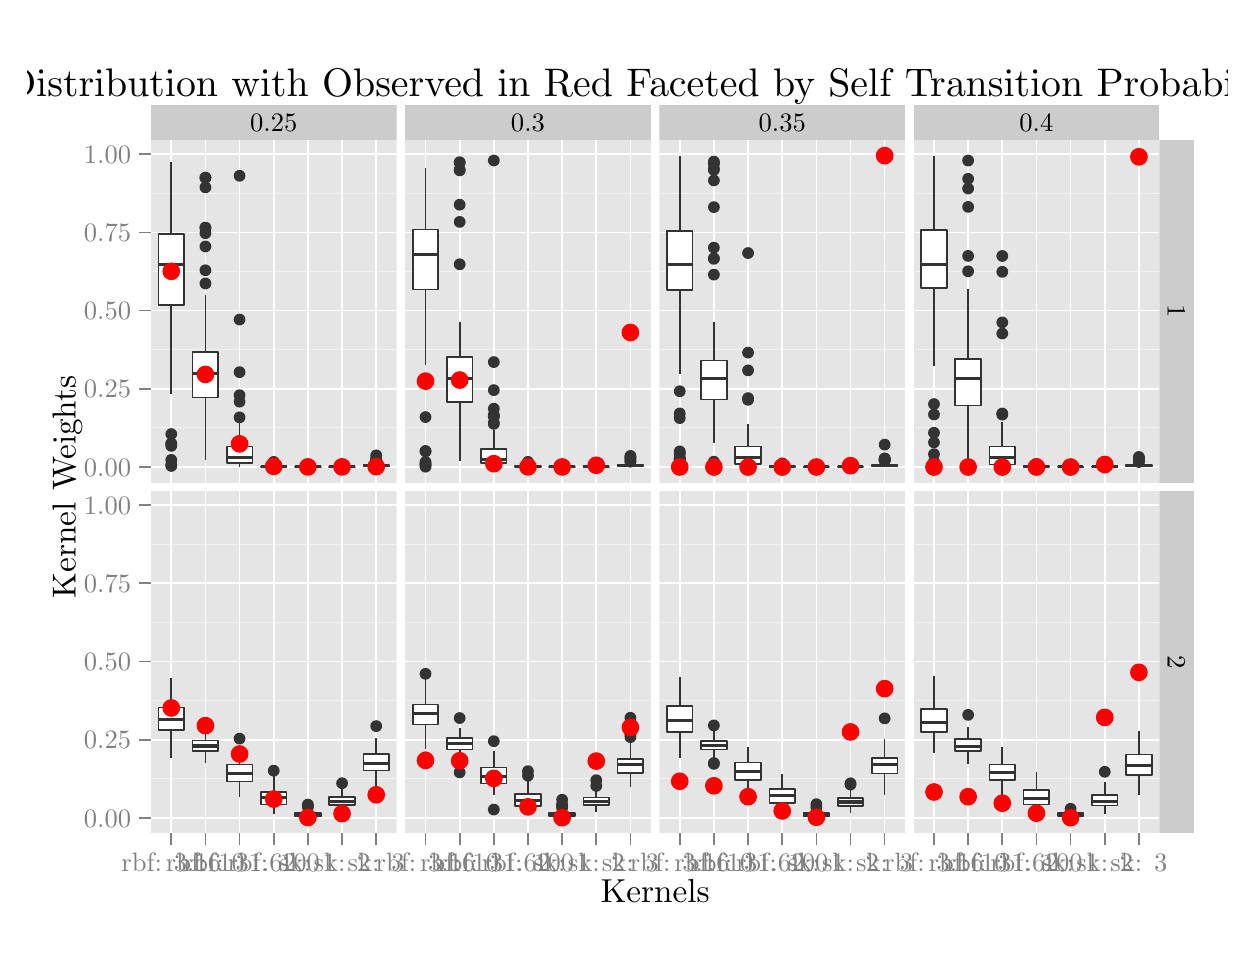
\begin{tikzpicture}[x=1pt,y=1pt]
\definecolor[named]{fillColor}{rgb}{1.00,1.00,1.00}
\path[use as bounding box,fill=fillColor,fill opacity=0.00] (0,0) rectangle (433.62,325.21);
\begin{scope}
\path[clip] (  0.00,  0.00) rectangle (433.62,325.21);
\definecolor[named]{drawColor}{rgb}{1.00,1.00,1.00}
\definecolor[named]{fillColor}{rgb}{1.00,1.00,1.00}

\path[draw=drawColor,line width= 0.6pt,line join=round,line cap=round,fill=fillColor] (  0.00,  0.00) rectangle (433.62,325.21);
\end{scope}
\begin{scope}
\path[clip] ( 44.49,284.60) rectangle (133.34,297.23);
\definecolor[named]{fillColor}{rgb}{0.80,0.80,0.80}

\path[fill=fillColor] ( 44.49,284.60) rectangle (133.34,297.23);
\definecolor[named]{drawColor}{rgb}{0.00,0.00,0.00}

\node[text=drawColor,anchor=base,inner sep=0pt, outer sep=0pt, scale=  0.96] at ( 88.91,287.61) {0.25};
\end{scope}
\begin{scope}
\path[clip] (136.35,284.60) rectangle (225.21,297.23);
\definecolor[named]{fillColor}{rgb}{0.80,0.80,0.80}

\path[fill=fillColor] (136.35,284.60) rectangle (225.21,297.23);
\definecolor[named]{drawColor}{rgb}{0.00,0.00,0.00}

\node[text=drawColor,anchor=base,inner sep=0pt, outer sep=0pt, scale=  0.96] at (180.78,287.61) {0.3};
\end{scope}
\begin{scope}
\path[clip] (228.22,284.60) rectangle (317.07,297.23);
\definecolor[named]{fillColor}{rgb}{0.80,0.80,0.80}

\path[fill=fillColor] (228.22,284.60) rectangle (317.07,297.23);
\definecolor[named]{drawColor}{rgb}{0.00,0.00,0.00}

\node[text=drawColor,anchor=base,inner sep=0pt, outer sep=0pt, scale=  0.96] at (272.65,287.61) {0.35};
\end{scope}
\begin{scope}
\path[clip] (320.09,284.60) rectangle (408.94,297.23);
\definecolor[named]{fillColor}{rgb}{0.80,0.80,0.80}

\path[fill=fillColor] (320.09,284.60) rectangle (408.94,297.23);
\definecolor[named]{drawColor}{rgb}{0.00,0.00,0.00}

\node[text=drawColor,anchor=base,inner sep=0pt, outer sep=0pt, scale=  0.96] at (364.51,287.61) {0.4};
\end{scope}
\begin{scope}
\path[clip] ( 44.49,160.82) rectangle (133.34,284.60);
\definecolor[named]{fillColor}{rgb}{0.90,0.90,0.90}

\path[fill=fillColor] ( 44.49,160.82) rectangle (133.34,284.60);
\definecolor[named]{drawColor}{rgb}{0.95,0.95,0.95}

\path[draw=drawColor,line width= 0.3pt,line join=round] ( 44.49,180.58) --
	(133.34,180.58);

\path[draw=drawColor,line width= 0.3pt,line join=round] ( 44.49,208.84) --
	(133.34,208.84);

\path[draw=drawColor,line width= 0.3pt,line join=round] ( 44.49,237.10) --
	(133.34,237.10);

\path[draw=drawColor,line width= 0.3pt,line join=round] ( 44.49,265.36) --
	(133.34,265.36);
\definecolor[named]{drawColor}{rgb}{1.00,1.00,1.00}

\path[draw=drawColor,line width= 0.6pt,line join=round] ( 44.49,166.45) --
	(133.34,166.45);

\path[draw=drawColor,line width= 0.6pt,line join=round] ( 44.49,194.71) --
	(133.34,194.71);

\path[draw=drawColor,line width= 0.6pt,line join=round] ( 44.49,222.97) --
	(133.34,222.97);

\path[draw=drawColor,line width= 0.6pt,line join=round] ( 44.49,251.23) --
	(133.34,251.23);

\path[draw=drawColor,line width= 0.6pt,line join=round] ( 44.49,279.49) --
	(133.34,279.49);

\path[draw=drawColor,line width= 0.6pt,line join=round] ( 51.89,160.82) --
	( 51.89,284.60);

\path[draw=drawColor,line width= 0.6pt,line join=round] ( 64.23,160.82) --
	( 64.23,284.60);

\path[draw=drawColor,line width= 0.6pt,line join=round] ( 76.57,160.82) --
	( 76.57,284.60);

\path[draw=drawColor,line width= 0.6pt,line join=round] ( 88.91,160.82) --
	( 88.91,284.60);

\path[draw=drawColor,line width= 0.6pt,line join=round] (101.25,160.82) --
	(101.25,284.60);

\path[draw=drawColor,line width= 0.6pt,line join=round] (113.60,160.82) --
	(113.60,284.60);

\path[draw=drawColor,line width= 0.6pt,line join=round] (125.94,160.82) --
	(125.94,284.60);
\definecolor[named]{fillColor}{rgb}{0.20,0.20,0.20}

\path[fill=fillColor] ( 51.89,169.02) circle (  2.13);

\path[fill=fillColor] ( 51.89,167.29) circle (  2.13);

\path[fill=fillColor] ( 51.89,178.35) circle (  2.13);

\path[fill=fillColor] ( 51.89,166.84) circle (  2.13);

\path[fill=fillColor] ( 51.89,174.92) circle (  2.13);

\path[fill=fillColor] ( 51.89,174.86) circle (  2.13);

\path[fill=fillColor] ( 51.89,174.09) circle (  2.13);
\definecolor[named]{drawColor}{rgb}{0.20,0.20,0.20}

\path[draw=drawColor,line width= 0.6pt,line join=round,fill=fillColor] ( 51.89,250.57) -- ( 51.89,276.78);

\path[draw=drawColor,line width= 0.6pt,line join=round,fill=fillColor] ( 51.89,225.08) -- ( 51.89,192.74);
\definecolor[named]{fillColor}{rgb}{1.00,1.00,1.00}

\path[draw=drawColor,line width= 0.6pt,line join=round,line cap=round,fill=fillColor] ( 47.26,250.57) --
	( 47.26,225.08) --
	( 56.52,225.08) --
	( 56.52,250.57) --
	( 47.26,250.57) --
	cycle;
\definecolor[named]{fillColor}{rgb}{0.20,0.20,0.20}

\path[draw=drawColor,line width= 1.1pt,line join=round,fill=fillColor] ( 47.26,239.51) -- ( 56.52,239.51);

\path[fill=fillColor] ( 64.23,250.94) circle (  2.13);

\path[fill=fillColor] ( 64.23,246.14) circle (  2.13);

\path[fill=fillColor] ( 64.23,232.79) circle (  2.13);

\path[fill=fillColor] ( 64.23,267.51) circle (  2.13);

\path[fill=fillColor] ( 64.23,270.96) circle (  2.13);

\path[fill=fillColor] ( 64.23,252.91) circle (  2.13);

\path[fill=fillColor] ( 64.23,271.03) circle (  2.13);

\path[fill=fillColor] ( 64.23,237.54) circle (  2.13);

\path[fill=fillColor] ( 64.23,252.94) circle (  2.13);

\path[draw=drawColor,line width= 0.6pt,line join=round,fill=fillColor] ( 64.23,208.07) -- ( 64.23,228.66);

\path[draw=drawColor,line width= 0.6pt,line join=round,fill=fillColor] ( 64.23,191.59) -- ( 64.23,169.10);
\definecolor[named]{fillColor}{rgb}{1.00,1.00,1.00}

\path[draw=drawColor,line width= 0.6pt,line join=round,line cap=round,fill=fillColor] ( 59.60,208.07) --
	( 59.60,191.59) --
	( 68.86,191.59) --
	( 68.86,208.07) --
	( 59.60,208.07) --
	cycle;
\definecolor[named]{fillColor}{rgb}{0.20,0.20,0.20}

\path[draw=drawColor,line width= 1.1pt,line join=round,fill=fillColor] ( 59.60,200.21) -- ( 68.86,200.21);

\path[fill=fillColor] ( 76.57,192.40) circle (  2.13);

\path[fill=fillColor] ( 76.57,219.74) circle (  2.13);

\path[fill=fillColor] ( 76.57,190.07) circle (  2.13);

\path[fill=fillColor] ( 76.57,184.39) circle (  2.13);

\path[fill=fillColor] ( 76.57,271.68) circle (  2.13);

\path[fill=fillColor] ( 76.57,200.73) circle (  2.13);

\path[draw=drawColor,line width= 0.6pt,line join=round,fill=fillColor] ( 76.57,173.85) -- ( 76.57,182.22);

\path[draw=drawColor,line width= 0.6pt,line join=round,fill=fillColor] ( 76.57,167.93) -- ( 76.57,166.46);
\definecolor[named]{fillColor}{rgb}{1.00,1.00,1.00}

\path[draw=drawColor,line width= 0.6pt,line join=round,line cap=round,fill=fillColor] ( 71.94,173.85) --
	( 71.94,167.93) --
	( 81.20,167.93) --
	( 81.20,173.85) --
	( 71.94,173.85) --
	cycle;
\definecolor[named]{fillColor}{rgb}{0.20,0.20,0.20}

\path[draw=drawColor,line width= 1.1pt,line join=round,fill=fillColor] ( 71.94,169.75) -- ( 81.20,169.75);

\path[fill=fillColor] ( 88.91,167.09) circle (  2.13);

\path[fill=fillColor] ( 88.91,167.06) circle (  2.13);

\path[fill=fillColor] ( 88.91,166.96) circle (  2.13);

\path[fill=fillColor] ( 88.91,166.97) circle (  2.13);

\path[fill=fillColor] ( 88.91,168.30) circle (  2.13);

\path[fill=fillColor] ( 88.91,167.37) circle (  2.13);

\path[fill=fillColor] ( 88.91,167.30) circle (  2.13);

\path[fill=fillColor] ( 88.91,167.20) circle (  2.13);

\path[fill=fillColor] ( 88.91,167.06) circle (  2.13);

\path[fill=fillColor] ( 88.91,166.99) circle (  2.13);

\path[draw=drawColor,line width= 0.6pt,line join=round,fill=fillColor] ( 88.91,166.69) -- ( 88.91,166.94);

\path[draw=drawColor,line width= 0.6pt,line join=round,fill=fillColor] ( 88.91,166.50) -- ( 88.91,166.45);
\definecolor[named]{fillColor}{rgb}{1.00,1.00,1.00}

\path[draw=drawColor,line width= 0.6pt,line join=round,line cap=round,fill=fillColor] ( 84.29,166.69) --
	( 84.29,166.50) --
	( 93.54,166.50) --
	( 93.54,166.69) --
	( 84.29,166.69) --
	cycle;
\definecolor[named]{fillColor}{rgb}{0.20,0.20,0.20}

\path[draw=drawColor,line width= 1.1pt,line join=round,fill=fillColor] ( 84.29,166.59) -- ( 93.54,166.59);

\path[fill=fillColor] (101.25,166.61) circle (  2.13);

\path[draw=drawColor,line width= 0.6pt,line join=round,fill=fillColor] (101.25,166.52) -- (101.25,166.58);

\path[draw=drawColor,line width= 0.6pt,line join=round,fill=fillColor] (101.25,166.46) -- (101.25,166.45);
\definecolor[named]{fillColor}{rgb}{1.00,1.00,1.00}

\path[draw=drawColor,line width= 0.6pt,line join=round,line cap=round,fill=fillColor] ( 96.63,166.52) --
	( 96.63,166.46) --
	(105.88,166.46) --
	(105.88,166.52) --
	( 96.63,166.52) --
	cycle;
\definecolor[named]{fillColor}{rgb}{0.20,0.20,0.20}

\path[draw=drawColor,line width= 1.1pt,line join=round,fill=fillColor] ( 96.63,166.50) -- (105.88,166.50);

\path[fill=fillColor] (113.60,166.69) circle (  2.13);

\path[draw=drawColor,line width= 0.6pt,line join=round,fill=fillColor] (113.60,166.56) -- (113.60,166.69);

\path[draw=drawColor,line width= 0.6pt,line join=round,fill=fillColor] (113.60,166.48) -- (113.60,166.45);
\definecolor[named]{fillColor}{rgb}{1.00,1.00,1.00}

\path[draw=drawColor,line width= 0.6pt,line join=round,line cap=round,fill=fillColor] (108.97,166.56) --
	(108.97,166.48) --
	(118.22,166.48) --
	(118.22,166.56) --
	(108.97,166.56) --
	cycle;
\definecolor[named]{fillColor}{rgb}{0.20,0.20,0.20}

\path[draw=drawColor,line width= 1.1pt,line join=round,fill=fillColor] (108.97,166.52) -- (118.22,166.52);

\path[fill=fillColor] (125.94,168.43) circle (  2.13);

\path[fill=fillColor] (125.94,168.93) circle (  2.13);

\path[fill=fillColor] (125.94,168.02) circle (  2.13);

\path[fill=fillColor] (125.94,168.41) circle (  2.13);

\path[fill=fillColor] (125.94,168.81) circle (  2.13);

\path[fill=fillColor] (125.94,170.66) circle (  2.13);

\path[fill=fillColor] (125.94,168.94) circle (  2.13);

\path[fill=fillColor] (125.94,169.49) circle (  2.13);

\path[draw=drawColor,line width= 0.6pt,line join=round,fill=fillColor] (125.94,167.11) -- (125.94,167.63);

\path[draw=drawColor,line width= 0.6pt,line join=round,fill=fillColor] (125.94,166.58) -- (125.94,166.45);
\definecolor[named]{fillColor}{rgb}{1.00,1.00,1.00}

\path[draw=drawColor,line width= 0.6pt,line join=round,line cap=round,fill=fillColor] (121.31,167.11) --
	(121.31,166.58) --
	(130.56,166.58) --
	(130.56,167.11) --
	(121.31,167.11) --
	cycle;
\definecolor[named]{fillColor}{rgb}{0.20,0.20,0.20}

\path[draw=drawColor,line width= 1.1pt,line join=round,fill=fillColor] (121.31,166.83) -- (130.56,166.83);
\definecolor[named]{fillColor}{rgb}{1.00,0.00,0.00}

\path[fill=fillColor] ( 51.89,237.17) circle (  3.20);

\path[fill=fillColor] ( 64.23,199.91) circle (  3.20);

\path[fill=fillColor] ( 76.57,174.82) circle (  3.20);

\path[fill=fillColor] ( 88.91,166.69) circle (  3.20);

\path[fill=fillColor] (101.25,166.49) circle (  3.20);

\path[fill=fillColor] (113.60,166.50) circle (  3.20);

\path[fill=fillColor] (125.94,166.59) circle (  3.20);
\end{scope}
\begin{scope}
\path[clip] ( 44.49, 34.03) rectangle (133.34,157.81);
\definecolor[named]{fillColor}{rgb}{0.90,0.90,0.90}

\path[fill=fillColor] ( 44.49, 34.03) rectangle (133.34,157.81);
\definecolor[named]{drawColor}{rgb}{0.95,0.95,0.95}

\path[draw=drawColor,line width= 0.3pt,line join=round] ( 44.49, 53.79) --
	(133.34, 53.79);

\path[draw=drawColor,line width= 0.3pt,line join=round] ( 44.49, 82.05) --
	(133.34, 82.05);

\path[draw=drawColor,line width= 0.3pt,line join=round] ( 44.49,110.31) --
	(133.34,110.31);

\path[draw=drawColor,line width= 0.3pt,line join=round] ( 44.49,138.57) --
	(133.34,138.57);
\definecolor[named]{drawColor}{rgb}{1.00,1.00,1.00}

\path[draw=drawColor,line width= 0.6pt,line join=round] ( 44.49, 39.66) --
	(133.34, 39.66);

\path[draw=drawColor,line width= 0.6pt,line join=round] ( 44.49, 67.92) --
	(133.34, 67.92);

\path[draw=drawColor,line width= 0.6pt,line join=round] ( 44.49, 96.18) --
	(133.34, 96.18);

\path[draw=drawColor,line width= 0.6pt,line join=round] ( 44.49,124.44) --
	(133.34,124.44);

\path[draw=drawColor,line width= 0.6pt,line join=round] ( 44.49,152.70) --
	(133.34,152.70);

\path[draw=drawColor,line width= 0.6pt,line join=round] ( 51.89, 34.03) --
	( 51.89,157.81);

\path[draw=drawColor,line width= 0.6pt,line join=round] ( 64.23, 34.03) --
	( 64.23,157.81);

\path[draw=drawColor,line width= 0.6pt,line join=round] ( 76.57, 34.03) --
	( 76.57,157.81);

\path[draw=drawColor,line width= 0.6pt,line join=round] ( 88.91, 34.03) --
	( 88.91,157.81);

\path[draw=drawColor,line width= 0.6pt,line join=round] (101.25, 34.03) --
	(101.25,157.81);

\path[draw=drawColor,line width= 0.6pt,line join=round] (113.60, 34.03) --
	(113.60,157.81);

\path[draw=drawColor,line width= 0.6pt,line join=round] (125.94, 34.03) --
	(125.94,157.81);
\definecolor[named]{drawColor}{rgb}{0.20,0.20,0.20}
\definecolor[named]{fillColor}{rgb}{0.20,0.20,0.20}

\path[draw=drawColor,line width= 0.6pt,line join=round,fill=fillColor] ( 51.89, 79.51) -- ( 51.89, 90.25);

\path[draw=drawColor,line width= 0.6pt,line join=round,fill=fillColor] ( 51.89, 71.53) -- ( 51.89, 61.30);
\definecolor[named]{fillColor}{rgb}{1.00,1.00,1.00}

\path[draw=drawColor,line width= 0.6pt,line join=round,line cap=round,fill=fillColor] ( 47.26, 79.51) --
	( 47.26, 71.53) --
	( 56.52, 71.53) --
	( 56.52, 79.51) --
	( 47.26, 79.51) --
	cycle;
\definecolor[named]{fillColor}{rgb}{0.20,0.20,0.20}

\path[draw=drawColor,line width= 1.1pt,line join=round,fill=fillColor] ( 47.26, 75.29) -- ( 56.52, 75.29);

\path[draw=drawColor,line width= 0.6pt,line join=round,fill=fillColor] ( 64.23, 67.67) -- ( 64.23, 72.12);

\path[draw=drawColor,line width= 0.6pt,line join=round,fill=fillColor] ( 64.23, 63.92) -- ( 64.23, 59.49);
\definecolor[named]{fillColor}{rgb}{1.00,1.00,1.00}

\path[draw=drawColor,line width= 0.6pt,line join=round,line cap=round,fill=fillColor] ( 59.60, 67.67) --
	( 59.60, 63.92) --
	( 68.86, 63.92) --
	( 68.86, 67.67) --
	( 59.60, 67.67) --
	cycle;
\definecolor[named]{fillColor}{rgb}{0.20,0.20,0.20}

\path[draw=drawColor,line width= 1.1pt,line join=round,fill=fillColor] ( 59.60, 65.64) -- ( 68.86, 65.64);

\path[fill=fillColor] ( 76.57, 68.31) circle (  2.13);

\path[draw=drawColor,line width= 0.6pt,line join=round,fill=fillColor] ( 76.57, 58.93) -- ( 76.57, 65.10);

\path[draw=drawColor,line width= 0.6pt,line join=round,fill=fillColor] ( 76.57, 52.86) -- ( 76.57, 47.35);
\definecolor[named]{fillColor}{rgb}{1.00,1.00,1.00}

\path[draw=drawColor,line width= 0.6pt,line join=round,line cap=round,fill=fillColor] ( 71.94, 58.93) --
	( 71.94, 52.86) --
	( 81.20, 52.86) --
	( 81.20, 58.93) --
	( 71.94, 58.93) --
	cycle;
\definecolor[named]{fillColor}{rgb}{0.20,0.20,0.20}

\path[draw=drawColor,line width= 1.1pt,line join=round,fill=fillColor] ( 71.94, 55.76) -- ( 81.20, 55.76);

\path[fill=fillColor] ( 88.91, 56.72) circle (  2.13);

\path[draw=drawColor,line width= 0.6pt,line join=round,fill=fillColor] ( 88.91, 48.95) -- ( 88.91, 55.48);

\path[draw=drawColor,line width= 0.6pt,line join=round,fill=fillColor] ( 88.91, 44.50) -- ( 88.91, 41.08);
\definecolor[named]{fillColor}{rgb}{1.00,1.00,1.00}

\path[draw=drawColor,line width= 0.6pt,line join=round,line cap=round,fill=fillColor] ( 84.29, 48.95) --
	( 84.29, 44.50) --
	( 93.54, 44.50) --
	( 93.54, 48.95) --
	( 84.29, 48.95) --
	cycle;
\definecolor[named]{fillColor}{rgb}{0.20,0.20,0.20}

\path[draw=drawColor,line width= 1.1pt,line join=round,fill=fillColor] ( 84.29, 46.90) -- ( 93.54, 46.90);

\path[fill=fillColor] (101.25, 43.86) circle (  2.13);

\path[fill=fillColor] (101.25, 44.48) circle (  2.13);

\path[fill=fillColor] (101.25, 43.68) circle (  2.13);

\path[draw=drawColor,line width= 0.6pt,line join=round,fill=fillColor] (101.25, 41.52) -- (101.25, 43.32);

\path[draw=drawColor,line width= 0.6pt,line join=round,fill=fillColor] (101.25, 40.22) -- (101.25, 39.75);
\definecolor[named]{fillColor}{rgb}{1.00,1.00,1.00}

\path[draw=drawColor,line width= 0.6pt,line join=round,line cap=round,fill=fillColor] ( 96.63, 41.52) --
	( 96.63, 40.22) --
	(105.88, 40.22) --
	(105.88, 41.52) --
	( 96.63, 41.52) --
	cycle;
\definecolor[named]{fillColor}{rgb}{0.20,0.20,0.20}

\path[draw=drawColor,line width= 1.1pt,line join=round,fill=fillColor] ( 96.63, 40.92) -- (105.88, 40.92);

\path[fill=fillColor] (113.60, 52.19) circle (  2.13);

\path[draw=drawColor,line width= 0.6pt,line join=round,fill=fillColor] (113.60, 47.21) -- (113.60, 51.49);

\path[draw=drawColor,line width= 0.6pt,line join=round,fill=fillColor] (113.60, 44.31) -- (113.60, 41.61);
\definecolor[named]{fillColor}{rgb}{1.00,1.00,1.00}

\path[draw=drawColor,line width= 0.6pt,line join=round,line cap=round,fill=fillColor] (108.97, 47.21) --
	(108.97, 44.31) --
	(118.22, 44.31) --
	(118.22, 47.21) --
	(108.97, 47.21) --
	cycle;
\definecolor[named]{fillColor}{rgb}{0.20,0.20,0.20}

\path[draw=drawColor,line width= 1.1pt,line join=round,fill=fillColor] (108.97, 45.45) -- (118.22, 45.45);

\path[fill=fillColor] (125.94, 72.83) circle (  2.13);

\path[draw=drawColor,line width= 0.6pt,line join=round,fill=fillColor] (125.94, 62.68) -- (125.94, 68.59);

\path[draw=drawColor,line width= 0.6pt,line join=round,fill=fillColor] (125.94, 56.77) -- (125.94, 50.73);
\definecolor[named]{fillColor}{rgb}{1.00,1.00,1.00}

\path[draw=drawColor,line width= 0.6pt,line join=round,line cap=round,fill=fillColor] (121.31, 62.68) --
	(121.31, 56.77) --
	(130.56, 56.77) --
	(130.56, 62.68) --
	(121.31, 62.68) --
	cycle;
\definecolor[named]{fillColor}{rgb}{0.20,0.20,0.20}

\path[draw=drawColor,line width= 1.1pt,line join=round,fill=fillColor] (121.31, 59.28) -- (130.56, 59.28);
\definecolor[named]{fillColor}{rgb}{1.00,0.00,0.00}

\path[fill=fillColor] ( 51.89, 79.39) circle (  3.20);

\path[fill=fillColor] ( 64.23, 73.01) circle (  3.20);

\path[fill=fillColor] ( 76.57, 62.75) circle (  3.20);

\path[fill=fillColor] ( 88.91, 46.47) circle (  3.20);

\path[fill=fillColor] (101.25, 39.80) circle (  3.20);

\path[fill=fillColor] (113.60, 41.22) circle (  3.20);

\path[fill=fillColor] (125.94, 48.02) circle (  3.20);
\end{scope}
\begin{scope}
\path[clip] (136.35,160.82) rectangle (225.21,284.60);
\definecolor[named]{fillColor}{rgb}{0.90,0.90,0.90}

\path[fill=fillColor] (136.35,160.82) rectangle (225.21,284.60);
\definecolor[named]{drawColor}{rgb}{0.95,0.95,0.95}

\path[draw=drawColor,line width= 0.3pt,line join=round] (136.35,180.58) --
	(225.21,180.58);

\path[draw=drawColor,line width= 0.3pt,line join=round] (136.35,208.84) --
	(225.21,208.84);

\path[draw=drawColor,line width= 0.3pt,line join=round] (136.35,237.10) --
	(225.21,237.10);

\path[draw=drawColor,line width= 0.3pt,line join=round] (136.35,265.36) --
	(225.21,265.36);
\definecolor[named]{drawColor}{rgb}{1.00,1.00,1.00}

\path[draw=drawColor,line width= 0.6pt,line join=round] (136.35,166.45) --
	(225.21,166.45);

\path[draw=drawColor,line width= 0.6pt,line join=round] (136.35,194.71) --
	(225.21,194.71);

\path[draw=drawColor,line width= 0.6pt,line join=round] (136.35,222.97) --
	(225.21,222.97);

\path[draw=drawColor,line width= 0.6pt,line join=round] (136.35,251.23) --
	(225.21,251.23);

\path[draw=drawColor,line width= 0.6pt,line join=round] (136.35,279.49) --
	(225.21,279.49);

\path[draw=drawColor,line width= 0.6pt,line join=round] (143.76,160.82) --
	(143.76,284.60);

\path[draw=drawColor,line width= 0.6pt,line join=round] (156.10,160.82) --
	(156.10,284.60);

\path[draw=drawColor,line width= 0.6pt,line join=round] (168.44,160.82) --
	(168.44,284.60);

\path[draw=drawColor,line width= 0.6pt,line join=round] (180.78,160.82) --
	(180.78,284.60);

\path[draw=drawColor,line width= 0.6pt,line join=round] (193.12,160.82) --
	(193.12,284.60);

\path[draw=drawColor,line width= 0.6pt,line join=round] (205.46,160.82) --
	(205.46,284.60);

\path[draw=drawColor,line width= 0.6pt,line join=round] (217.80,160.82) --
	(217.80,284.60);
\definecolor[named]{fillColor}{rgb}{0.20,0.20,0.20}

\path[fill=fillColor] (143.76,172.07) circle (  2.13);

\path[fill=fillColor] (143.76,166.57) circle (  2.13);

\path[fill=fillColor] (143.76,167.33) circle (  2.13);

\path[fill=fillColor] (143.76,167.25) circle (  2.13);

\path[fill=fillColor] (143.76,172.25) circle (  2.13);

\path[fill=fillColor] (143.76,184.49) circle (  2.13);

\path[fill=fillColor] (143.76,168.30) circle (  2.13);

\path[fill=fillColor] (143.76,167.77) circle (  2.13);
\definecolor[named]{drawColor}{rgb}{0.20,0.20,0.20}

\path[draw=drawColor,line width= 0.6pt,line join=round,fill=fillColor] (143.76,252.22) -- (143.76,274.35);

\path[draw=drawColor,line width= 0.6pt,line join=round,fill=fillColor] (143.76,230.59) -- (143.76,203.36);
\definecolor[named]{fillColor}{rgb}{1.00,1.00,1.00}

\path[draw=drawColor,line width= 0.6pt,line join=round,line cap=round,fill=fillColor] (139.13,252.22) --
	(139.13,230.59) --
	(148.38,230.59) --
	(148.38,252.22) --
	(139.13,252.22) --
	cycle;
\definecolor[named]{fillColor}{rgb}{0.20,0.20,0.20}

\path[draw=drawColor,line width= 1.1pt,line join=round,fill=fillColor] (139.13,243.27) -- (148.38,243.27);

\path[fill=fillColor] (156.10,255.03) circle (  2.13);

\path[fill=fillColor] (156.10,276.55) circle (  2.13);

\path[fill=fillColor] (156.10,273.89) circle (  2.13);

\path[fill=fillColor] (156.10,273.64) circle (  2.13);

\path[fill=fillColor] (156.10,261.24) circle (  2.13);

\path[fill=fillColor] (156.10,239.70) circle (  2.13);

\path[fill=fillColor] (156.10,276.50) circle (  2.13);

\path[draw=drawColor,line width= 0.6pt,line join=round,fill=fillColor] (156.10,206.25) -- (156.10,218.84);

\path[draw=drawColor,line width= 0.6pt,line join=round,fill=fillColor] (156.10,189.95) -- (156.10,168.56);
\definecolor[named]{fillColor}{rgb}{1.00,1.00,1.00}

\path[draw=drawColor,line width= 0.6pt,line join=round,line cap=round,fill=fillColor] (151.47,206.25) --
	(151.47,189.95) --
	(160.73,189.95) --
	(160.73,206.25) --
	(151.47,206.25) --
	cycle;
\definecolor[named]{fillColor}{rgb}{0.20,0.20,0.20}

\path[draw=drawColor,line width= 1.1pt,line join=round,fill=fillColor] (151.47,198.27) -- (160.73,198.27);

\path[fill=fillColor] (168.44,194.24) circle (  2.13);

\path[fill=fillColor] (168.44,185.24) circle (  2.13);

\path[fill=fillColor] (168.44,277.21) circle (  2.13);

\path[fill=fillColor] (168.44,182.40) circle (  2.13);

\path[fill=fillColor] (168.44,187.51) circle (  2.13);

\path[fill=fillColor] (168.44,182.04) circle (  2.13);

\path[fill=fillColor] (168.44,184.72) circle (  2.13);

\path[fill=fillColor] (168.44,204.37) circle (  2.13);

\path[fill=fillColor] (168.44,184.77) circle (  2.13);

\path[draw=drawColor,line width= 0.6pt,line join=round,fill=fillColor] (168.44,173.02) -- (168.44,179.96);

\path[draw=drawColor,line width= 0.6pt,line join=round,fill=fillColor] (168.44,167.99) -- (168.44,166.46);
\definecolor[named]{fillColor}{rgb}{1.00,1.00,1.00}

\path[draw=drawColor,line width= 0.6pt,line join=round,line cap=round,fill=fillColor] (163.81,173.02) --
	(163.81,167.99) --
	(173.07,167.99) --
	(173.07,173.02) --
	(163.81,173.02) --
	cycle;
\definecolor[named]{fillColor}{rgb}{0.20,0.20,0.20}

\path[draw=drawColor,line width= 1.1pt,line join=round,fill=fillColor] (163.81,169.28) -- (173.07,169.28);

\path[fill=fillColor] (180.78,168.31) circle (  2.13);

\path[fill=fillColor] (180.78,166.97) circle (  2.13);

\path[fill=fillColor] (180.78,167.00) circle (  2.13);

\path[fill=fillColor] (180.78,167.08) circle (  2.13);

\path[fill=fillColor] (180.78,166.97) circle (  2.13);

\path[fill=fillColor] (180.78,167.28) circle (  2.13);

\path[fill=fillColor] (180.78,166.96) circle (  2.13);

\path[fill=fillColor] (180.78,167.69) circle (  2.13);

\path[fill=fillColor] (180.78,167.04) circle (  2.13);

\path[fill=fillColor] (180.78,167.31) circle (  2.13);

\path[fill=fillColor] (180.78,167.59) circle (  2.13);

\path[fill=fillColor] (180.78,167.04) circle (  2.13);

\path[draw=drawColor,line width= 0.6pt,line join=round,fill=fillColor] (180.78,166.70) -- (180.78,166.91);

\path[draw=drawColor,line width= 0.6pt,line join=round,fill=fillColor] (180.78,166.54) -- (180.78,166.45);
\definecolor[named]{fillColor}{rgb}{1.00,1.00,1.00}

\path[draw=drawColor,line width= 0.6pt,line join=round,line cap=round,fill=fillColor] (176.15,166.70) --
	(176.15,166.54) --
	(185.41,166.54) --
	(185.41,166.70) --
	(176.15,166.70) --
	cycle;
\definecolor[named]{fillColor}{rgb}{0.20,0.20,0.20}

\path[draw=drawColor,line width= 1.1pt,line join=round,fill=fillColor] (176.15,166.59) -- (185.41,166.59);

\path[draw=drawColor,line width= 0.6pt,line join=round,fill=fillColor] (193.12,166.52) -- (193.12,166.59);

\path[draw=drawColor,line width= 0.6pt,line join=round,fill=fillColor] (193.12,166.47) -- (193.12,166.45);
\definecolor[named]{fillColor}{rgb}{1.00,1.00,1.00}

\path[draw=drawColor,line width= 0.6pt,line join=round,line cap=round,fill=fillColor] (188.49,166.52) --
	(188.49,166.47) --
	(197.75,166.47) --
	(197.75,166.52) --
	(188.49,166.52) --
	cycle;
\definecolor[named]{fillColor}{rgb}{0.20,0.20,0.20}

\path[draw=drawColor,line width= 1.1pt,line join=round,fill=fillColor] (188.49,166.50) -- (197.75,166.50);

\path[draw=drawColor,line width= 0.6pt,line join=round,fill=fillColor] (205.46,166.57) -- (205.46,166.68);

\path[draw=drawColor,line width= 0.6pt,line join=round,fill=fillColor] (205.46,166.49) -- (205.46,166.45);
\definecolor[named]{fillColor}{rgb}{1.00,1.00,1.00}

\path[draw=drawColor,line width= 0.6pt,line join=round,line cap=round,fill=fillColor] (200.83,166.57) --
	(200.83,166.49) --
	(210.09,166.49) --
	(210.09,166.57) --
	(200.83,166.57) --
	cycle;
\definecolor[named]{fillColor}{rgb}{0.20,0.20,0.20}

\path[draw=drawColor,line width= 1.1pt,line join=round,fill=fillColor] (200.83,166.54) -- (210.09,166.54);

\path[fill=fillColor] (217.80,168.56) circle (  2.13);

\path[fill=fillColor] (217.80,168.39) circle (  2.13);

\path[fill=fillColor] (217.80,169.34) circle (  2.13);

\path[fill=fillColor] (217.80,170.18) circle (  2.13);

\path[fill=fillColor] (217.80,170.46) circle (  2.13);

\path[fill=fillColor] (217.80,169.72) circle (  2.13);

\path[draw=drawColor,line width= 0.6pt,line join=round,fill=fillColor] (217.80,167.32) -- (217.80,168.28);

\path[draw=drawColor,line width= 0.6pt,line join=round,fill=fillColor] (217.80,166.64) -- (217.80,166.45);
\definecolor[named]{fillColor}{rgb}{1.00,1.00,1.00}

\path[draw=drawColor,line width= 0.6pt,line join=round,line cap=round,fill=fillColor] (213.17,167.32) --
	(213.17,166.64) --
	(222.43,166.64) --
	(222.43,167.32) --
	(213.17,167.32) --
	cycle;
\definecolor[named]{fillColor}{rgb}{0.20,0.20,0.20}

\path[draw=drawColor,line width= 1.1pt,line join=round,fill=fillColor] (213.17,166.90) -- (222.43,166.90);
\definecolor[named]{fillColor}{rgb}{1.00,0.00,0.00}

\path[fill=fillColor] (143.76,197.48) circle (  3.20);

\path[fill=fillColor] (156.10,197.88) circle (  3.20);

\path[fill=fillColor] (168.44,167.66) circle (  3.20);

\path[fill=fillColor] (180.78,166.51) circle (  3.20);

\path[fill=fillColor] (193.12,166.48) circle (  3.20);

\path[fill=fillColor] (205.46,167.08) circle (  3.20);

\path[fill=fillColor] (217.80,215.07) circle (  3.20);
\end{scope}
\begin{scope}
\path[clip] (136.35, 34.03) rectangle (225.21,157.81);
\definecolor[named]{fillColor}{rgb}{0.90,0.90,0.90}

\path[fill=fillColor] (136.35, 34.03) rectangle (225.21,157.81);
\definecolor[named]{drawColor}{rgb}{0.95,0.95,0.95}

\path[draw=drawColor,line width= 0.3pt,line join=round] (136.35, 53.79) --
	(225.21, 53.79);

\path[draw=drawColor,line width= 0.3pt,line join=round] (136.35, 82.05) --
	(225.21, 82.05);

\path[draw=drawColor,line width= 0.3pt,line join=round] (136.35,110.31) --
	(225.21,110.31);

\path[draw=drawColor,line width= 0.3pt,line join=round] (136.35,138.57) --
	(225.21,138.57);
\definecolor[named]{drawColor}{rgb}{1.00,1.00,1.00}

\path[draw=drawColor,line width= 0.6pt,line join=round] (136.35, 39.66) --
	(225.21, 39.66);

\path[draw=drawColor,line width= 0.6pt,line join=round] (136.35, 67.92) --
	(225.21, 67.92);

\path[draw=drawColor,line width= 0.6pt,line join=round] (136.35, 96.18) --
	(225.21, 96.18);

\path[draw=drawColor,line width= 0.6pt,line join=round] (136.35,124.44) --
	(225.21,124.44);

\path[draw=drawColor,line width= 0.6pt,line join=round] (136.35,152.70) --
	(225.21,152.70);

\path[draw=drawColor,line width= 0.6pt,line join=round] (143.76, 34.03) --
	(143.76,157.81);

\path[draw=drawColor,line width= 0.6pt,line join=round] (156.10, 34.03) --
	(156.10,157.81);

\path[draw=drawColor,line width= 0.6pt,line join=round] (168.44, 34.03) --
	(168.44,157.81);

\path[draw=drawColor,line width= 0.6pt,line join=round] (180.78, 34.03) --
	(180.78,157.81);

\path[draw=drawColor,line width= 0.6pt,line join=round] (193.12, 34.03) --
	(193.12,157.81);

\path[draw=drawColor,line width= 0.6pt,line join=round] (205.46, 34.03) --
	(205.46,157.81);

\path[draw=drawColor,line width= 0.6pt,line join=round] (217.80, 34.03) --
	(217.80,157.81);
\definecolor[named]{fillColor}{rgb}{0.20,0.20,0.20}

\path[fill=fillColor] (143.76, 61.50) circle (  2.13);

\path[fill=fillColor] (143.76, 91.73) circle (  2.13);
\definecolor[named]{drawColor}{rgb}{0.20,0.20,0.20}

\path[draw=drawColor,line width= 0.6pt,line join=round,fill=fillColor] (143.76, 80.60) -- (143.76, 91.05);

\path[draw=drawColor,line width= 0.6pt,line join=round,fill=fillColor] (143.76, 73.37) -- (143.76, 64.72);
\definecolor[named]{fillColor}{rgb}{1.00,1.00,1.00}

\path[draw=drawColor,line width= 0.6pt,line join=round,line cap=round,fill=fillColor] (139.13, 80.60) --
	(139.13, 73.37) --
	(148.38, 73.37) --
	(148.38, 80.60) --
	(139.13, 80.60) --
	cycle;
\definecolor[named]{fillColor}{rgb}{0.20,0.20,0.20}

\path[draw=drawColor,line width= 1.1pt,line join=round,fill=fillColor] (139.13, 77.52) -- (148.38, 77.52);

\path[fill=fillColor] (156.10, 75.74) circle (  2.13);

\path[fill=fillColor] (156.10, 56.11) circle (  2.13);

\path[draw=drawColor,line width= 0.6pt,line join=round,fill=fillColor] (156.10, 68.60) -- (156.10, 72.19);

\path[draw=drawColor,line width= 0.6pt,line join=round,fill=fillColor] (156.10, 64.32) -- (156.10, 58.55);
\definecolor[named]{fillColor}{rgb}{1.00,1.00,1.00}

\path[draw=drawColor,line width= 0.6pt,line join=round,line cap=round,fill=fillColor] (151.47, 68.60) --
	(151.47, 64.32) --
	(160.73, 64.32) --
	(160.73, 68.60) --
	(151.47, 68.60) --
	cycle;
\definecolor[named]{fillColor}{rgb}{0.20,0.20,0.20}

\path[draw=drawColor,line width= 1.1pt,line join=round,fill=fillColor] (151.47, 66.65) -- (160.73, 66.65);

\path[fill=fillColor] (168.44, 67.39) circle (  2.13);

\path[fill=fillColor] (168.44, 42.67) circle (  2.13);

\path[draw=drawColor,line width= 0.6pt,line join=round,fill=fillColor] (168.44, 57.84) -- (168.44, 63.89);

\path[draw=drawColor,line width= 0.6pt,line join=round,fill=fillColor] (168.44, 52.13) -- (168.44, 47.83);
\definecolor[named]{fillColor}{rgb}{1.00,1.00,1.00}

\path[draw=drawColor,line width= 0.6pt,line join=round,line cap=round,fill=fillColor] (163.81, 57.84) --
	(163.81, 52.13) --
	(173.07, 52.13) --
	(173.07, 57.84) --
	(163.81, 57.84) --
	cycle;
\definecolor[named]{fillColor}{rgb}{0.20,0.20,0.20}

\path[draw=drawColor,line width= 1.1pt,line join=round,fill=fillColor] (163.81, 54.65) -- (173.07, 54.65);

\path[fill=fillColor] (180.78, 56.55) circle (  2.13);

\path[fill=fillColor] (180.78, 54.90) circle (  2.13);

\path[draw=drawColor,line width= 0.6pt,line join=round,fill=fillColor] (180.78, 48.36) -- (180.78, 53.64);

\path[draw=drawColor,line width= 0.6pt,line join=round,fill=fillColor] (180.78, 44.02) -- (180.78, 40.73);
\definecolor[named]{fillColor}{rgb}{1.00,1.00,1.00}

\path[draw=drawColor,line width= 0.6pt,line join=round,line cap=round,fill=fillColor] (176.15, 48.36) --
	(176.15, 44.02) --
	(185.41, 44.02) --
	(185.41, 48.36) --
	(176.15, 48.36) --
	cycle;
\definecolor[named]{fillColor}{rgb}{0.20,0.20,0.20}

\path[draw=drawColor,line width= 1.1pt,line join=round,fill=fillColor] (176.15, 45.78) -- (185.41, 45.78);

\path[fill=fillColor] (193.12, 43.35) circle (  2.13);

\path[fill=fillColor] (193.12, 44.37) circle (  2.13);

\path[fill=fillColor] (193.12, 44.42) circle (  2.13);

\path[fill=fillColor] (193.12, 46.22) circle (  2.13);

\path[fill=fillColor] (193.12, 43.66) circle (  2.13);

\path[draw=drawColor,line width= 0.6pt,line join=round,fill=fillColor] (193.12, 41.42) -- (193.12, 43.14);

\path[draw=drawColor,line width= 0.6pt,line join=round,fill=fillColor] (193.12, 40.24) -- (193.12, 39.69);
\definecolor[named]{fillColor}{rgb}{1.00,1.00,1.00}

\path[draw=drawColor,line width= 0.6pt,line join=round,line cap=round,fill=fillColor] (188.49, 41.42) --
	(188.49, 40.24) --
	(197.75, 40.24) --
	(197.75, 41.42) --
	(188.49, 41.42) --
	cycle;
\definecolor[named]{fillColor}{rgb}{0.20,0.20,0.20}

\path[draw=drawColor,line width= 1.1pt,line join=round,fill=fillColor] (188.49, 40.78) -- (197.75, 40.78);

\path[fill=fillColor] (205.46, 51.21) circle (  2.13);

\path[fill=fillColor] (205.46, 53.29) circle (  2.13);

\path[draw=drawColor,line width= 0.6pt,line join=round,fill=fillColor] (205.46, 47.02) -- (205.46, 51.11);

\path[draw=drawColor,line width= 0.6pt,line join=round,fill=fillColor] (205.46, 44.27) -- (205.46, 41.88);
\definecolor[named]{fillColor}{rgb}{1.00,1.00,1.00}

\path[draw=drawColor,line width= 0.6pt,line join=round,line cap=round,fill=fillColor] (200.83, 47.02) --
	(200.83, 44.27) --
	(210.09, 44.27) --
	(210.09, 47.02) --
	(200.83, 47.02) --
	cycle;
\definecolor[named]{fillColor}{rgb}{0.20,0.20,0.20}

\path[draw=drawColor,line width= 1.1pt,line join=round,fill=fillColor] (200.83, 45.56) -- (210.09, 45.56);

\path[fill=fillColor] (217.80, 68.84) circle (  2.13);

\path[fill=fillColor] (217.80, 69.89) circle (  2.13);

\path[fill=fillColor] (217.80, 70.24) circle (  2.13);

\path[fill=fillColor] (217.80, 73.98) circle (  2.13);

\path[fill=fillColor] (217.80, 75.84) circle (  2.13);

\path[draw=drawColor,line width= 0.6pt,line join=round,fill=fillColor] (217.80, 61.05) -- (217.80, 68.62);

\path[draw=drawColor,line width= 0.6pt,line join=round,fill=fillColor] (217.80, 55.93) -- (217.80, 50.73);
\definecolor[named]{fillColor}{rgb}{1.00,1.00,1.00}

\path[draw=drawColor,line width= 0.6pt,line join=round,line cap=round,fill=fillColor] (213.17, 61.05) --
	(213.17, 55.93) --
	(222.43, 55.93) --
	(222.43, 61.05) --
	(213.17, 61.05) --
	cycle;
\definecolor[named]{fillColor}{rgb}{0.20,0.20,0.20}

\path[draw=drawColor,line width= 1.1pt,line join=round,fill=fillColor] (213.17, 58.84) -- (222.43, 58.84);
\definecolor[named]{fillColor}{rgb}{1.00,0.00,0.00}

\path[fill=fillColor] (143.76, 60.44) circle (  3.20);

\path[fill=fillColor] (156.10, 60.31) circle (  3.20);

\path[fill=fillColor] (168.44, 53.94) circle (  3.20);

\path[fill=fillColor] (180.78, 43.66) circle (  3.20);

\path[fill=fillColor] (193.12, 39.74) circle (  3.20);

\path[fill=fillColor] (205.46, 60.19) circle (  3.20);

\path[fill=fillColor] (217.80, 72.38) circle (  3.20);
\end{scope}
\begin{scope}
\path[clip] (228.22,160.82) rectangle (317.07,284.60);
\definecolor[named]{fillColor}{rgb}{0.90,0.90,0.90}

\path[fill=fillColor] (228.22,160.82) rectangle (317.07,284.60);
\definecolor[named]{drawColor}{rgb}{0.95,0.95,0.95}

\path[draw=drawColor,line width= 0.3pt,line join=round] (228.22,180.58) --
	(317.07,180.58);

\path[draw=drawColor,line width= 0.3pt,line join=round] (228.22,208.84) --
	(317.07,208.84);

\path[draw=drawColor,line width= 0.3pt,line join=round] (228.22,237.10) --
	(317.07,237.10);

\path[draw=drawColor,line width= 0.3pt,line join=round] (228.22,265.36) --
	(317.07,265.36);
\definecolor[named]{drawColor}{rgb}{1.00,1.00,1.00}

\path[draw=drawColor,line width= 0.6pt,line join=round] (228.22,166.45) --
	(317.07,166.45);

\path[draw=drawColor,line width= 0.6pt,line join=round] (228.22,194.71) --
	(317.07,194.71);

\path[draw=drawColor,line width= 0.6pt,line join=round] (228.22,222.97) --
	(317.07,222.97);

\path[draw=drawColor,line width= 0.6pt,line join=round] (228.22,251.23) --
	(317.07,251.23);

\path[draw=drawColor,line width= 0.6pt,line join=round] (228.22,279.49) --
	(317.07,279.49);

\path[draw=drawColor,line width= 0.6pt,line join=round] (235.62,160.82) --
	(235.62,284.60);

\path[draw=drawColor,line width= 0.6pt,line join=round] (247.96,160.82) --
	(247.96,284.60);

\path[draw=drawColor,line width= 0.6pt,line join=round] (260.31,160.82) --
	(260.31,284.60);

\path[draw=drawColor,line width= 0.6pt,line join=round] (272.65,160.82) --
	(272.65,284.60);

\path[draw=drawColor,line width= 0.6pt,line join=round] (284.99,160.82) --
	(284.99,284.60);

\path[draw=drawColor,line width= 0.6pt,line join=round] (297.33,160.82) --
	(297.33,284.60);

\path[draw=drawColor,line width= 0.6pt,line join=round] (309.67,160.82) --
	(309.67,284.60);
\definecolor[named]{fillColor}{rgb}{0.20,0.20,0.20}

\path[fill=fillColor] (235.62,169.31) circle (  2.13);

\path[fill=fillColor] (235.62,169.56) circle (  2.13);

\path[fill=fillColor] (235.62,172.10) circle (  2.13);

\path[fill=fillColor] (235.62,169.72) circle (  2.13);

\path[fill=fillColor] (235.62,184.13) circle (  2.13);

\path[fill=fillColor] (235.62,193.83) circle (  2.13);

\path[fill=fillColor] (235.62,185.82) circle (  2.13);

\path[fill=fillColor] (235.62,169.09) circle (  2.13);

\path[fill=fillColor] (235.62,167.02) circle (  2.13);

\path[fill=fillColor] (235.62,171.16) circle (  2.13);

\path[fill=fillColor] (235.62,171.62) circle (  2.13);
\definecolor[named]{drawColor}{rgb}{0.20,0.20,0.20}

\path[draw=drawColor,line width= 0.6pt,line join=round,fill=fillColor] (235.62,251.64) -- (235.62,278.92);

\path[draw=drawColor,line width= 0.6pt,line join=round,fill=fillColor] (235.62,230.41) -- (235.62,200.12);
\definecolor[named]{fillColor}{rgb}{1.00,1.00,1.00}

\path[draw=drawColor,line width= 0.6pt,line join=round,line cap=round,fill=fillColor] (231.00,251.64) --
	(231.00,230.41) --
	(240.25,230.41) --
	(240.25,251.64) --
	(231.00,251.64) --
	cycle;
\definecolor[named]{fillColor}{rgb}{0.20,0.20,0.20}

\path[draw=drawColor,line width= 1.1pt,line join=round,fill=fillColor] (231.00,239.57) -- (240.25,239.57);

\path[fill=fillColor] (247.96,241.67) circle (  2.13);

\path[fill=fillColor] (247.96,276.25) circle (  2.13);

\path[fill=fillColor] (247.96,166.99) circle (  2.13);

\path[fill=fillColor] (247.96,273.80) circle (  2.13);

\path[fill=fillColor] (247.96,276.04) circle (  2.13);

\path[fill=fillColor] (247.96,260.36) circle (  2.13);

\path[fill=fillColor] (247.96,241.90) circle (  2.13);

\path[fill=fillColor] (247.96,235.97) circle (  2.13);

\path[fill=fillColor] (247.96,276.82) circle (  2.13);

\path[fill=fillColor] (247.96,168.38) circle (  2.13);

\path[fill=fillColor] (247.96,270.02) circle (  2.13);

\path[fill=fillColor] (247.96,245.70) circle (  2.13);

\path[fill=fillColor] (247.96,274.19) circle (  2.13);

\path[draw=drawColor,line width= 0.6pt,line join=round,fill=fillColor] (247.96,204.93) -- (247.96,218.74);

\path[draw=drawColor,line width= 0.6pt,line join=round,fill=fillColor] (247.96,190.86) -- (247.96,174.98);
\definecolor[named]{fillColor}{rgb}{1.00,1.00,1.00}

\path[draw=drawColor,line width= 0.6pt,line join=round,line cap=round,fill=fillColor] (243.34,204.93) --
	(243.34,190.86) --
	(252.59,190.86) --
	(252.59,204.93) --
	(243.34,204.93) --
	cycle;
\definecolor[named]{fillColor}{rgb}{0.20,0.20,0.20}

\path[draw=drawColor,line width= 1.1pt,line join=round,fill=fillColor] (243.34,198.41) -- (252.59,198.41);

\path[fill=fillColor] (260.31,201.38) circle (  2.13);

\path[fill=fillColor] (260.31,191.35) circle (  2.13);

\path[fill=fillColor] (260.31,207.79) circle (  2.13);

\path[fill=fillColor] (260.31,190.73) circle (  2.13);

\path[fill=fillColor] (260.31,243.77) circle (  2.13);

\path[draw=drawColor,line width= 0.6pt,line join=round,fill=fillColor] (260.31,173.90) -- (260.31,182.15);

\path[draw=drawColor,line width= 0.6pt,line join=round,fill=fillColor] (260.31,167.47) -- (260.31,166.45);
\definecolor[named]{fillColor}{rgb}{1.00,1.00,1.00}

\path[draw=drawColor,line width= 0.6pt,line join=round,line cap=round,fill=fillColor] (255.68,173.90) --
	(255.68,167.47) --
	(264.93,167.47) --
	(264.93,173.90) --
	(255.68,173.90) --
	cycle;
\definecolor[named]{fillColor}{rgb}{0.20,0.20,0.20}

\path[draw=drawColor,line width= 1.1pt,line join=round,fill=fillColor] (255.68,170.01) -- (264.93,170.01);

\path[fill=fillColor] (272.65,167.67) circle (  2.13);

\path[fill=fillColor] (272.65,167.38) circle (  2.13);

\path[fill=fillColor] (272.65,167.14) circle (  2.13);

\path[fill=fillColor] (272.65,167.22) circle (  2.13);

\path[fill=fillColor] (272.65,167.75) circle (  2.13);

\path[draw=drawColor,line width= 0.6pt,line join=round,fill=fillColor] (272.65,166.73) -- (272.65,167.03);

\path[draw=drawColor,line width= 0.6pt,line join=round,fill=fillColor] (272.65,166.53) -- (272.65,166.45);
\definecolor[named]{fillColor}{rgb}{1.00,1.00,1.00}

\path[draw=drawColor,line width= 0.6pt,line join=round,line cap=round,fill=fillColor] (268.02,166.73) --
	(268.02,166.53) --
	(277.27,166.53) --
	(277.27,166.73) --
	(268.02,166.73) --
	cycle;
\definecolor[named]{fillColor}{rgb}{0.20,0.20,0.20}

\path[draw=drawColor,line width= 1.1pt,line join=round,fill=fillColor] (268.02,166.59) -- (277.27,166.59);

\path[draw=drawColor,line width= 0.6pt,line join=round,fill=fillColor] (284.99,166.53) -- (284.99,166.58);

\path[draw=drawColor,line width= 0.6pt,line join=round,fill=fillColor] (284.99,166.47) -- (284.99,166.45);
\definecolor[named]{fillColor}{rgb}{1.00,1.00,1.00}

\path[draw=drawColor,line width= 0.6pt,line join=round,line cap=round,fill=fillColor] (280.36,166.53) --
	(280.36,166.47) --
	(289.62,166.47) --
	(289.62,166.53) --
	(280.36,166.53) --
	cycle;
\definecolor[named]{fillColor}{rgb}{0.20,0.20,0.20}

\path[draw=drawColor,line width= 1.1pt,line join=round,fill=fillColor] (280.36,166.50) -- (289.62,166.50);

\path[fill=fillColor] (297.33,166.77) circle (  2.13);

\path[fill=fillColor] (297.33,166.77) circle (  2.13);

\path[draw=drawColor,line width= 0.6pt,line join=round,fill=fillColor] (297.33,166.59) -- (297.33,166.73);

\path[draw=drawColor,line width= 0.6pt,line join=round,fill=fillColor] (297.33,166.49) -- (297.33,166.45);
\definecolor[named]{fillColor}{rgb}{1.00,1.00,1.00}

\path[draw=drawColor,line width= 0.6pt,line join=round,line cap=round,fill=fillColor] (292.70,166.59) --
	(292.70,166.49) --
	(301.96,166.49) --
	(301.96,166.59) --
	(292.70,166.59) --
	cycle;
\definecolor[named]{fillColor}{rgb}{0.20,0.20,0.20}

\path[draw=drawColor,line width= 1.1pt,line join=round,fill=fillColor] (292.70,166.54) -- (301.96,166.54);

\path[fill=fillColor] (309.67,169.51) circle (  2.13);

\path[fill=fillColor] (309.67,174.54) circle (  2.13);

\path[fill=fillColor] (309.67,169.14) circle (  2.13);

\path[fill=fillColor] (309.67,168.99) circle (  2.13);

\path[fill=fillColor] (309.67,168.84) circle (  2.13);

\path[fill=fillColor] (309.67,169.51) circle (  2.13);

\path[fill=fillColor] (309.67,169.17) circle (  2.13);

\path[fill=fillColor] (309.67,168.90) circle (  2.13);

\path[fill=fillColor] (309.67,168.91) circle (  2.13);

\path[draw=drawColor,line width= 0.6pt,line join=round,fill=fillColor] (309.67,167.29) -- (309.67,167.84);

\path[draw=drawColor,line width= 0.6pt,line join=round,fill=fillColor] (309.67,166.64) -- (309.67,166.45);
\definecolor[named]{fillColor}{rgb}{1.00,1.00,1.00}

\path[draw=drawColor,line width= 0.6pt,line join=round,line cap=round,fill=fillColor] (305.04,167.29) --
	(305.04,166.64) --
	(314.30,166.64) --
	(314.30,167.29) --
	(305.04,167.29) --
	cycle;
\definecolor[named]{fillColor}{rgb}{0.20,0.20,0.20}

\path[draw=drawColor,line width= 1.1pt,line join=round,fill=fillColor] (305.04,166.91) -- (314.30,166.91);
\definecolor[named]{fillColor}{rgb}{1.00,0.00,0.00}

\path[fill=fillColor] (235.62,166.46) circle (  3.20);

\path[fill=fillColor] (247.96,166.45) circle (  3.20);

\path[fill=fillColor] (260.31,166.45) circle (  3.20);

\path[fill=fillColor] (272.65,166.45) circle (  3.20);

\path[fill=fillColor] (284.99,166.45) circle (  3.20);

\path[fill=fillColor] (297.33,166.94) circle (  3.20);

\path[fill=fillColor] (309.67,278.97) circle (  3.20);
\end{scope}
\begin{scope}
\path[clip] (228.22, 34.03) rectangle (317.07,157.81);
\definecolor[named]{fillColor}{rgb}{0.90,0.90,0.90}

\path[fill=fillColor] (228.22, 34.03) rectangle (317.07,157.81);
\definecolor[named]{drawColor}{rgb}{0.95,0.95,0.95}

\path[draw=drawColor,line width= 0.3pt,line join=round] (228.22, 53.79) --
	(317.07, 53.79);

\path[draw=drawColor,line width= 0.3pt,line join=round] (228.22, 82.05) --
	(317.07, 82.05);

\path[draw=drawColor,line width= 0.3pt,line join=round] (228.22,110.31) --
	(317.07,110.31);

\path[draw=drawColor,line width= 0.3pt,line join=round] (228.22,138.57) --
	(317.07,138.57);
\definecolor[named]{drawColor}{rgb}{1.00,1.00,1.00}

\path[draw=drawColor,line width= 0.6pt,line join=round] (228.22, 39.66) --
	(317.07, 39.66);

\path[draw=drawColor,line width= 0.6pt,line join=round] (228.22, 67.92) --
	(317.07, 67.92);

\path[draw=drawColor,line width= 0.6pt,line join=round] (228.22, 96.18) --
	(317.07, 96.18);

\path[draw=drawColor,line width= 0.6pt,line join=round] (228.22,124.44) --
	(317.07,124.44);

\path[draw=drawColor,line width= 0.6pt,line join=round] (228.22,152.70) --
	(317.07,152.70);

\path[draw=drawColor,line width= 0.6pt,line join=round] (235.62, 34.03) --
	(235.62,157.81);

\path[draw=drawColor,line width= 0.6pt,line join=round] (247.96, 34.03) --
	(247.96,157.81);

\path[draw=drawColor,line width= 0.6pt,line join=round] (260.31, 34.03) --
	(260.31,157.81);

\path[draw=drawColor,line width= 0.6pt,line join=round] (272.65, 34.03) --
	(272.65,157.81);

\path[draw=drawColor,line width= 0.6pt,line join=round] (284.99, 34.03) --
	(284.99,157.81);

\path[draw=drawColor,line width= 0.6pt,line join=round] (297.33, 34.03) --
	(297.33,157.81);

\path[draw=drawColor,line width= 0.6pt,line join=round] (309.67, 34.03) --
	(309.67,157.81);
\definecolor[named]{drawColor}{rgb}{0.20,0.20,0.20}
\definecolor[named]{fillColor}{rgb}{0.20,0.20,0.20}

\path[draw=drawColor,line width= 0.6pt,line join=round,fill=fillColor] (235.62, 79.99) -- (235.62, 90.70);

\path[draw=drawColor,line width= 0.6pt,line join=round,fill=fillColor] (235.62, 70.68) -- (235.62, 61.43);
\definecolor[named]{fillColor}{rgb}{1.00,1.00,1.00}

\path[draw=drawColor,line width= 0.6pt,line join=round,line cap=round,fill=fillColor] (231.00, 79.99) --
	(231.00, 70.68) --
	(240.25, 70.68) --
	(240.25, 79.99) --
	(231.00, 79.99) --
	cycle;
\definecolor[named]{fillColor}{rgb}{0.20,0.20,0.20}

\path[draw=drawColor,line width= 1.1pt,line join=round,fill=fillColor] (231.00, 74.92) -- (240.25, 74.92);

\path[fill=fillColor] (247.96, 59.18) circle (  2.13);

\path[fill=fillColor] (247.96, 59.47) circle (  2.13);

\path[fill=fillColor] (247.96, 73.08) circle (  2.13);

\path[draw=drawColor,line width= 0.6pt,line join=round,fill=fillColor] (247.96, 67.47) -- (247.96, 71.07);

\path[draw=drawColor,line width= 0.6pt,line join=round,fill=fillColor] (247.96, 64.32) -- (247.96, 59.73);
\definecolor[named]{fillColor}{rgb}{1.00,1.00,1.00}

\path[draw=drawColor,line width= 0.6pt,line join=round,line cap=round,fill=fillColor] (243.34, 67.47) --
	(243.34, 64.32) --
	(252.59, 64.32) --
	(252.59, 67.47) --
	(243.34, 67.47) --
	cycle;
\definecolor[named]{fillColor}{rgb}{0.20,0.20,0.20}

\path[draw=drawColor,line width= 1.1pt,line join=round,fill=fillColor] (243.34, 65.88) -- (252.59, 65.88);

\path[draw=drawColor,line width= 0.6pt,line join=round,fill=fillColor] (260.31, 59.66) -- (260.31, 65.43);

\path[draw=drawColor,line width= 0.6pt,line join=round,fill=fillColor] (260.31, 53.32) -- (260.31, 46.69);
\definecolor[named]{fillColor}{rgb}{1.00,1.00,1.00}

\path[draw=drawColor,line width= 0.6pt,line join=round,line cap=round,fill=fillColor] (255.68, 59.66) --
	(255.68, 53.32) --
	(264.93, 53.32) --
	(264.93, 59.66) --
	(255.68, 59.66) --
	cycle;
\definecolor[named]{fillColor}{rgb}{0.20,0.20,0.20}

\path[draw=drawColor,line width= 1.1pt,line join=round,fill=fillColor] (255.68, 56.27) -- (264.93, 56.27);

\path[draw=drawColor,line width= 0.6pt,line join=round,fill=fillColor] (272.65, 50.11) -- (272.65, 55.54);

\path[draw=drawColor,line width= 0.6pt,line join=round,fill=fillColor] (272.65, 45.15) -- (272.65, 41.27);
\definecolor[named]{fillColor}{rgb}{1.00,1.00,1.00}

\path[draw=drawColor,line width= 0.6pt,line join=round,line cap=round,fill=fillColor] (268.02, 50.11) --
	(268.02, 45.15) --
	(277.27, 45.15) --
	(277.27, 50.11) --
	(268.02, 50.11) --
	cycle;
\definecolor[named]{fillColor}{rgb}{0.20,0.20,0.20}

\path[draw=drawColor,line width= 1.1pt,line join=round,fill=fillColor] (268.02, 47.88) -- (277.27, 47.88);

\path[fill=fillColor] (284.99, 43.51) circle (  2.13);

\path[fill=fillColor] (284.99, 44.63) circle (  2.13);

\path[draw=drawColor,line width= 0.6pt,line join=round,fill=fillColor] (284.99, 41.37) -- (284.99, 42.77);

\path[draw=drawColor,line width= 0.6pt,line join=round,fill=fillColor] (284.99, 40.18) -- (284.99, 39.68);
\definecolor[named]{fillColor}{rgb}{1.00,1.00,1.00}

\path[draw=drawColor,line width= 0.6pt,line join=round,line cap=round,fill=fillColor] (280.36, 41.37) --
	(280.36, 40.18) --
	(289.62, 40.18) --
	(289.62, 41.37) --
	(280.36, 41.37) --
	cycle;
\definecolor[named]{fillColor}{rgb}{0.20,0.20,0.20}

\path[draw=drawColor,line width= 1.1pt,line join=round,fill=fillColor] (280.36, 40.85) -- (289.62, 40.85);

\path[fill=fillColor] (297.33, 51.69) circle (  2.13);

\path[fill=fillColor] (297.33, 52.15) circle (  2.13);

\path[draw=drawColor,line width= 0.6pt,line join=round,fill=fillColor] (297.33, 46.94) -- (297.33, 50.75);

\path[draw=drawColor,line width= 0.6pt,line join=round,fill=fillColor] (297.33, 43.98) -- (297.33, 41.40);
\definecolor[named]{fillColor}{rgb}{1.00,1.00,1.00}

\path[draw=drawColor,line width= 0.6pt,line join=round,line cap=round,fill=fillColor] (292.70, 46.94) --
	(292.70, 43.98) --
	(301.96, 43.98) --
	(301.96, 46.94) --
	(292.70, 46.94) --
	cycle;
\definecolor[named]{fillColor}{rgb}{0.20,0.20,0.20}

\path[draw=drawColor,line width= 1.1pt,line join=round,fill=fillColor] (292.70, 45.40) -- (301.96, 45.40);

\path[fill=fillColor] (309.67, 75.63) circle (  2.13);

\path[draw=drawColor,line width= 0.6pt,line join=round,fill=fillColor] (309.67, 61.38) -- (309.67, 68.06);

\path[draw=drawColor,line width= 0.6pt,line join=round,fill=fillColor] (309.67, 55.72) -- (309.67, 47.88);
\definecolor[named]{fillColor}{rgb}{1.00,1.00,1.00}

\path[draw=drawColor,line width= 0.6pt,line join=round,line cap=round,fill=fillColor] (305.04, 61.38) --
	(305.04, 55.72) --
	(314.30, 55.72) --
	(314.30, 61.38) --
	(305.04, 61.38) --
	cycle;
\definecolor[named]{fillColor}{rgb}{0.20,0.20,0.20}

\path[draw=drawColor,line width= 1.1pt,line join=round,fill=fillColor] (305.04, 58.88) -- (314.30, 58.88);
\definecolor[named]{fillColor}{rgb}{1.00,0.00,0.00}

\path[fill=fillColor] (235.62, 52.90) circle (  3.20);

\path[fill=fillColor] (247.96, 51.26) circle (  3.20);

\path[fill=fillColor] (260.31, 47.33) circle (  3.20);

\path[fill=fillColor] (272.65, 42.18) circle (  3.20);

\path[fill=fillColor] (284.99, 39.90) circle (  3.20);

\path[fill=fillColor] (297.33, 70.73) circle (  3.20);

\path[fill=fillColor] (309.67, 86.37) circle (  3.20);
\end{scope}
\begin{scope}
\path[clip] (320.09,160.82) rectangle (408.94,284.60);
\definecolor[named]{fillColor}{rgb}{0.90,0.90,0.90}

\path[fill=fillColor] (320.09,160.82) rectangle (408.94,284.60);
\definecolor[named]{drawColor}{rgb}{0.95,0.95,0.95}

\path[draw=drawColor,line width= 0.3pt,line join=round] (320.09,180.58) --
	(408.94,180.58);

\path[draw=drawColor,line width= 0.3pt,line join=round] (320.09,208.84) --
	(408.94,208.84);

\path[draw=drawColor,line width= 0.3pt,line join=round] (320.09,237.10) --
	(408.94,237.10);

\path[draw=drawColor,line width= 0.3pt,line join=round] (320.09,265.36) --
	(408.94,265.36);
\definecolor[named]{drawColor}{rgb}{1.00,1.00,1.00}

\path[draw=drawColor,line width= 0.6pt,line join=round] (320.09,166.45) --
	(408.94,166.45);

\path[draw=drawColor,line width= 0.6pt,line join=round] (320.09,194.71) --
	(408.94,194.71);

\path[draw=drawColor,line width= 0.6pt,line join=round] (320.09,222.97) --
	(408.94,222.97);

\path[draw=drawColor,line width= 0.6pt,line join=round] (320.09,251.23) --
	(408.94,251.23);

\path[draw=drawColor,line width= 0.6pt,line join=round] (320.09,279.49) --
	(408.94,279.49);

\path[draw=drawColor,line width= 0.6pt,line join=round] (327.49,160.82) --
	(327.49,284.60);

\path[draw=drawColor,line width= 0.6pt,line join=round] (339.83,160.82) --
	(339.83,284.60);

\path[draw=drawColor,line width= 0.6pt,line join=round] (352.17,160.82) --
	(352.17,284.60);

\path[draw=drawColor,line width= 0.6pt,line join=round] (364.51,160.82) --
	(364.51,284.60);

\path[draw=drawColor,line width= 0.6pt,line join=round] (376.85,160.82) --
	(376.85,284.60);

\path[draw=drawColor,line width= 0.6pt,line join=round] (389.20,160.82) --
	(389.20,284.60);

\path[draw=drawColor,line width= 0.6pt,line join=round] (401.54,160.82) --
	(401.54,284.60);
\definecolor[named]{fillColor}{rgb}{0.20,0.20,0.20}

\path[fill=fillColor] (327.49,166.97) circle (  2.13);

\path[fill=fillColor] (327.49,168.39) circle (  2.13);

\path[fill=fillColor] (327.49,189.20) circle (  2.13);

\path[fill=fillColor] (327.49,178.82) circle (  2.13);

\path[fill=fillColor] (327.49,175.33) circle (  2.13);

\path[fill=fillColor] (327.49,166.51) circle (  2.13);

\path[fill=fillColor] (327.49,185.43) circle (  2.13);

\path[fill=fillColor] (327.49,171.09) circle (  2.13);
\definecolor[named]{drawColor}{rgb}{0.20,0.20,0.20}

\path[draw=drawColor,line width= 0.6pt,line join=round,fill=fillColor] (327.49,252.18) -- (327.49,278.92);

\path[draw=drawColor,line width= 0.6pt,line join=round,fill=fillColor] (327.49,231.17) -- (327.49,202.92);
\definecolor[named]{fillColor}{rgb}{1.00,1.00,1.00}

\path[draw=drawColor,line width= 0.6pt,line join=round,line cap=round,fill=fillColor] (322.86,252.18) --
	(322.86,231.17) --
	(332.12,231.17) --
	(332.12,252.18) --
	(322.86,252.18) --
	cycle;
\definecolor[named]{fillColor}{rgb}{0.20,0.20,0.20}

\path[draw=drawColor,line width= 1.1pt,line join=round,fill=fillColor] (322.86,239.66) -- (332.12,239.66);

\path[fill=fillColor] (339.83,277.18) circle (  2.13);

\path[fill=fillColor] (339.83,267.08) circle (  2.13);

\path[fill=fillColor] (339.83,242.73) circle (  2.13);

\path[fill=fillColor] (339.83,270.58) circle (  2.13);

\path[fill=fillColor] (339.83,260.45) circle (  2.13);

\path[fill=fillColor] (339.83,237.18) circle (  2.13);

\path[draw=drawColor,line width= 0.6pt,line join=round,fill=fillColor] (339.83,205.56) -- (339.83,230.71);

\path[draw=drawColor,line width= 0.6pt,line join=round,fill=fillColor] (339.83,188.72) -- (339.83,166.99);
\definecolor[named]{fillColor}{rgb}{1.00,1.00,1.00}

\path[draw=drawColor,line width= 0.6pt,line join=round,line cap=round,fill=fillColor] (335.20,205.56) --
	(335.20,188.72) --
	(344.46,188.72) --
	(344.46,205.56) --
	(335.20,205.56) --
	cycle;
\definecolor[named]{fillColor}{rgb}{0.20,0.20,0.20}

\path[draw=drawColor,line width= 1.1pt,line join=round,fill=fillColor] (335.20,198.37) -- (344.46,198.37);

\path[fill=fillColor] (352.17,185.81) circle (  2.13);

\path[fill=fillColor] (352.17,214.69) circle (  2.13);

\path[fill=fillColor] (352.17,236.98) circle (  2.13);

\path[fill=fillColor] (352.17,185.38) circle (  2.13);

\path[fill=fillColor] (352.17,242.71) circle (  2.13);

\path[fill=fillColor] (352.17,218.70) circle (  2.13);

\path[draw=drawColor,line width= 0.6pt,line join=round,fill=fillColor] (352.17,173.87) -- (352.17,182.57);

\path[draw=drawColor,line width= 0.6pt,line join=round,fill=fillColor] (352.17,167.41) -- (352.17,166.45);
\definecolor[named]{fillColor}{rgb}{1.00,1.00,1.00}

\path[draw=drawColor,line width= 0.6pt,line join=round,line cap=round,fill=fillColor] (347.54,173.87) --
	(347.54,167.41) --
	(356.80,167.41) --
	(356.80,173.87) --
	(347.54,173.87) --
	cycle;
\definecolor[named]{fillColor}{rgb}{0.20,0.20,0.20}

\path[draw=drawColor,line width= 1.1pt,line join=round,fill=fillColor] (347.54,169.83) -- (356.80,169.83);

\path[fill=fillColor] (364.51,167.16) circle (  2.13);

\path[fill=fillColor] (364.51,166.99) circle (  2.13);

\path[fill=fillColor] (364.51,167.03) circle (  2.13);

\path[fill=fillColor] (364.51,167.19) circle (  2.13);

\path[fill=fillColor] (364.51,167.02) circle (  2.13);

\path[fill=fillColor] (364.51,167.34) circle (  2.13);

\path[fill=fillColor] (364.51,167.60) circle (  2.13);

\path[draw=drawColor,line width= 0.6pt,line join=round,fill=fillColor] (364.51,166.71) -- (364.51,166.98);

\path[draw=drawColor,line width= 0.6pt,line join=round,fill=fillColor] (364.51,166.53) -- (364.51,166.45);
\definecolor[named]{fillColor}{rgb}{1.00,1.00,1.00}

\path[draw=drawColor,line width= 0.6pt,line join=round,line cap=round,fill=fillColor] (359.89,166.71) --
	(359.89,166.53) --
	(369.14,166.53) --
	(369.14,166.71) --
	(359.89,166.71) --
	cycle;
\definecolor[named]{fillColor}{rgb}{0.20,0.20,0.20}

\path[draw=drawColor,line width= 1.1pt,line join=round,fill=fillColor] (359.89,166.60) -- (369.14,166.60);

\path[fill=fillColor] (376.85,166.62) circle (  2.13);

\path[draw=drawColor,line width= 0.6pt,line join=round,fill=fillColor] (376.85,166.53) -- (376.85,166.57);

\path[draw=drawColor,line width= 0.6pt,line join=round,fill=fillColor] (376.85,166.47) -- (376.85,166.45);
\definecolor[named]{fillColor}{rgb}{1.00,1.00,1.00}

\path[draw=drawColor,line width= 0.6pt,line join=round,line cap=round,fill=fillColor] (372.23,166.53) --
	(372.23,166.47) --
	(381.48,166.47) --
	(381.48,166.53) --
	(372.23,166.53) --
	cycle;
\definecolor[named]{fillColor}{rgb}{0.20,0.20,0.20}

\path[draw=drawColor,line width= 1.1pt,line join=round,fill=fillColor] (372.23,166.51) -- (381.48,166.51);

\path[fill=fillColor] (389.20,166.99) circle (  2.13);

\path[draw=drawColor,line width= 0.6pt,line join=round,fill=fillColor] (389.20,166.58) -- (389.20,166.70);

\path[draw=drawColor,line width= 0.6pt,line join=round,fill=fillColor] (389.20,166.48) -- (389.20,166.45);
\definecolor[named]{fillColor}{rgb}{1.00,1.00,1.00}

\path[draw=drawColor,line width= 0.6pt,line join=round,line cap=round,fill=fillColor] (384.57,166.58) --
	(384.57,166.48) --
	(393.82,166.48) --
	(393.82,166.58) --
	(384.57,166.58) --
	cycle;
\definecolor[named]{fillColor}{rgb}{0.20,0.20,0.20}

\path[draw=drawColor,line width= 1.1pt,line join=round,fill=fillColor] (384.57,166.54) -- (393.82,166.54);

\path[fill=fillColor] (401.54,168.86) circle (  2.13);

\path[fill=fillColor] (401.54,168.42) circle (  2.13);

\path[fill=fillColor] (401.54,168.70) circle (  2.13);

\path[fill=fillColor] (401.54,169.49) circle (  2.13);

\path[fill=fillColor] (401.54,169.11) circle (  2.13);

\path[fill=fillColor] (401.54,169.56) circle (  2.13);

\path[fill=fillColor] (401.54,168.31) circle (  2.13);

\path[fill=fillColor] (401.54,170.09) circle (  2.13);

\path[draw=drawColor,line width= 0.6pt,line join=round,fill=fillColor] (401.54,167.25) -- (401.54,168.19);

\path[draw=drawColor,line width= 0.6pt,line join=round,fill=fillColor] (401.54,166.59) -- (401.54,166.45);
\definecolor[named]{fillColor}{rgb}{1.00,1.00,1.00}

\path[draw=drawColor,line width= 0.6pt,line join=round,line cap=round,fill=fillColor] (396.91,167.25) --
	(396.91,166.59) --
	(406.16,166.59) --
	(406.16,167.25) --
	(396.91,167.25) --
	cycle;
\definecolor[named]{fillColor}{rgb}{0.20,0.20,0.20}

\path[draw=drawColor,line width= 1.1pt,line join=round,fill=fillColor] (396.91,166.90) -- (406.16,166.90);
\definecolor[named]{fillColor}{rgb}{1.00,0.00,0.00}

\path[fill=fillColor] (327.49,166.45) circle (  3.20);

\path[fill=fillColor] (339.83,166.45) circle (  3.20);

\path[fill=fillColor] (352.17,166.45) circle (  3.20);

\path[fill=fillColor] (364.51,166.45) circle (  3.20);

\path[fill=fillColor] (376.85,166.45) circle (  3.20);

\path[fill=fillColor] (389.20,167.36) circle (  3.20);

\path[fill=fillColor] (401.54,278.55) circle (  3.20);
\end{scope}
\begin{scope}
\path[clip] (320.09, 34.03) rectangle (408.94,157.81);
\definecolor[named]{fillColor}{rgb}{0.90,0.90,0.90}

\path[fill=fillColor] (320.09, 34.03) rectangle (408.94,157.81);
\definecolor[named]{drawColor}{rgb}{0.95,0.95,0.95}

\path[draw=drawColor,line width= 0.3pt,line join=round] (320.09, 53.79) --
	(408.94, 53.79);

\path[draw=drawColor,line width= 0.3pt,line join=round] (320.09, 82.05) --
	(408.94, 82.05);

\path[draw=drawColor,line width= 0.3pt,line join=round] (320.09,110.31) --
	(408.94,110.31);

\path[draw=drawColor,line width= 0.3pt,line join=round] (320.09,138.57) --
	(408.94,138.57);
\definecolor[named]{drawColor}{rgb}{1.00,1.00,1.00}

\path[draw=drawColor,line width= 0.6pt,line join=round] (320.09, 39.66) --
	(408.94, 39.66);

\path[draw=drawColor,line width= 0.6pt,line join=round] (320.09, 67.92) --
	(408.94, 67.92);

\path[draw=drawColor,line width= 0.6pt,line join=round] (320.09, 96.18) --
	(408.94, 96.18);

\path[draw=drawColor,line width= 0.6pt,line join=round] (320.09,124.44) --
	(408.94,124.44);

\path[draw=drawColor,line width= 0.6pt,line join=round] (320.09,152.70) --
	(408.94,152.70);

\path[draw=drawColor,line width= 0.6pt,line join=round] (327.49, 34.03) --
	(327.49,157.81);

\path[draw=drawColor,line width= 0.6pt,line join=round] (339.83, 34.03) --
	(339.83,157.81);

\path[draw=drawColor,line width= 0.6pt,line join=round] (352.17, 34.03) --
	(352.17,157.81);

\path[draw=drawColor,line width= 0.6pt,line join=round] (364.51, 34.03) --
	(364.51,157.81);

\path[draw=drawColor,line width= 0.6pt,line join=round] (376.85, 34.03) --
	(376.85,157.81);

\path[draw=drawColor,line width= 0.6pt,line join=round] (389.20, 34.03) --
	(389.20,157.81);

\path[draw=drawColor,line width= 0.6pt,line join=round] (401.54, 34.03) --
	(401.54,157.81);
\definecolor[named]{drawColor}{rgb}{0.20,0.20,0.20}
\definecolor[named]{fillColor}{rgb}{0.20,0.20,0.20}

\path[draw=drawColor,line width= 0.6pt,line join=round,fill=fillColor] (327.49, 78.90) -- (327.49, 90.84);

\path[draw=drawColor,line width= 0.6pt,line join=round,fill=fillColor] (327.49, 70.60) -- (327.49, 63.10);
\definecolor[named]{fillColor}{rgb}{1.00,1.00,1.00}

\path[draw=drawColor,line width= 0.6pt,line join=round,line cap=round,fill=fillColor] (322.86, 78.90) --
	(322.86, 70.60) --
	(332.12, 70.60) --
	(332.12, 78.90) --
	(322.86, 78.90) --
	cycle;
\definecolor[named]{fillColor}{rgb}{0.20,0.20,0.20}

\path[draw=drawColor,line width= 1.1pt,line join=round,fill=fillColor] (322.86, 74.28) -- (332.12, 74.28);

\path[fill=fillColor] (339.83, 76.89) circle (  2.13);

\path[draw=drawColor,line width= 0.6pt,line join=round,fill=fillColor] (339.83, 68.10) -- (339.83, 72.68);

\path[draw=drawColor,line width= 0.6pt,line join=round,fill=fillColor] (339.83, 63.90) -- (339.83, 59.27);
\definecolor[named]{fillColor}{rgb}{1.00,1.00,1.00}

\path[draw=drawColor,line width= 0.6pt,line join=round,line cap=round,fill=fillColor] (335.20, 68.10) --
	(335.20, 63.90) --
	(344.46, 63.90) --
	(344.46, 68.10) --
	(335.20, 68.10) --
	cycle;
\definecolor[named]{fillColor}{rgb}{0.20,0.20,0.20}

\path[draw=drawColor,line width= 1.1pt,line join=round,fill=fillColor] (335.20, 65.53) -- (344.46, 65.53);

\path[draw=drawColor,line width= 0.6pt,line join=round,fill=fillColor] (352.17, 58.96) -- (352.17, 65.12);

\path[draw=drawColor,line width= 0.6pt,line join=round,fill=fillColor] (352.17, 53.26) -- (352.17, 46.28);
\definecolor[named]{fillColor}{rgb}{1.00,1.00,1.00}

\path[draw=drawColor,line width= 0.6pt,line join=round,line cap=round,fill=fillColor] (347.54, 58.96) --
	(347.54, 53.26) --
	(356.80, 53.26) --
	(356.80, 58.96) --
	(347.54, 58.96) --
	cycle;
\definecolor[named]{fillColor}{rgb}{0.20,0.20,0.20}

\path[draw=drawColor,line width= 1.1pt,line join=round,fill=fillColor] (347.54, 56.16) -- (356.80, 56.16);

\path[draw=drawColor,line width= 0.6pt,line join=round,fill=fillColor] (364.51, 49.85) -- (364.51, 56.37);

\path[draw=drawColor,line width= 0.6pt,line join=round,fill=fillColor] (364.51, 44.51) -- (364.51, 41.24);
\definecolor[named]{fillColor}{rgb}{1.00,1.00,1.00}

\path[draw=drawColor,line width= 0.6pt,line join=round,line cap=round,fill=fillColor] (359.89, 49.85) --
	(359.89, 44.51) --
	(369.14, 44.51) --
	(369.14, 49.85) --
	(359.89, 49.85) --
	cycle;
\definecolor[named]{fillColor}{rgb}{0.20,0.20,0.20}

\path[draw=drawColor,line width= 1.1pt,line join=round,fill=fillColor] (359.89, 46.68) -- (369.14, 46.68);

\path[fill=fillColor] (376.85, 42.95) circle (  2.13);

\path[draw=drawColor,line width= 0.6pt,line join=round,fill=fillColor] (376.85, 41.32) -- (376.85, 42.79);

\path[draw=drawColor,line width= 0.6pt,line join=round,fill=fillColor] (376.85, 40.30) -- (376.85, 39.69);
\definecolor[named]{fillColor}{rgb}{1.00,1.00,1.00}

\path[draw=drawColor,line width= 0.6pt,line join=round,line cap=round,fill=fillColor] (372.23, 41.32) --
	(372.23, 40.30) --
	(381.48, 40.30) --
	(381.48, 41.32) --
	(372.23, 41.32) --
	cycle;
\definecolor[named]{fillColor}{rgb}{0.20,0.20,0.20}

\path[draw=drawColor,line width= 1.1pt,line join=round,fill=fillColor] (372.23, 40.64) -- (381.48, 40.64);

\path[fill=fillColor] (389.20, 56.32) circle (  2.13);

\path[draw=drawColor,line width= 0.6pt,line join=round,fill=fillColor] (389.20, 47.89) -- (389.20, 52.57);

\path[draw=drawColor,line width= 0.6pt,line join=round,fill=fillColor] (389.20, 44.20) -- (389.20, 41.14);
\definecolor[named]{fillColor}{rgb}{1.00,1.00,1.00}

\path[draw=drawColor,line width= 0.6pt,line join=round,line cap=round,fill=fillColor] (384.57, 47.89) --
	(384.57, 44.20) --
	(393.82, 44.20) --
	(393.82, 47.89) --
	(384.57, 47.89) --
	cycle;
\definecolor[named]{fillColor}{rgb}{0.20,0.20,0.20}

\path[draw=drawColor,line width= 1.1pt,line join=round,fill=fillColor] (384.57, 45.51) -- (393.82, 45.51);

\path[draw=drawColor,line width= 0.6pt,line join=round,fill=fillColor] (401.54, 62.52) -- (401.54, 71.13);

\path[draw=drawColor,line width= 0.6pt,line join=round,fill=fillColor] (401.54, 55.18) -- (401.54, 47.98);
\definecolor[named]{fillColor}{rgb}{1.00,1.00,1.00}

\path[draw=drawColor,line width= 0.6pt,line join=round,line cap=round,fill=fillColor] (396.91, 62.52) --
	(396.91, 55.18) --
	(406.16, 55.18) --
	(406.16, 62.52) --
	(396.91, 62.52) --
	cycle;
\definecolor[named]{fillColor}{rgb}{0.20,0.20,0.20}

\path[draw=drawColor,line width= 1.1pt,line join=round,fill=fillColor] (396.91, 58.69) -- (406.16, 58.69);
\definecolor[named]{fillColor}{rgb}{1.00,0.00,0.00}

\path[fill=fillColor] (327.49, 49.02) circle (  3.20);

\path[fill=fillColor] (339.83, 47.33) circle (  3.20);

\path[fill=fillColor] (352.17, 44.98) circle (  3.20);

\path[fill=fillColor] (364.51, 41.36) circle (  3.20);

\path[fill=fillColor] (376.85, 39.74) circle (  3.20);

\path[fill=fillColor] (389.20, 75.98) circle (  3.20);

\path[fill=fillColor] (401.54, 92.26) circle (  3.20);
\end{scope}
\begin{scope}
\path[clip] (  0.00,  0.00) rectangle (433.62,325.21);
\definecolor[named]{drawColor}{rgb}{0.50,0.50,0.50}

\node[text=drawColor,anchor=base east,inner sep=0pt, outer sep=0pt, scale=  0.96] at ( 37.37,163.14) {0.00};

\node[text=drawColor,anchor=base east,inner sep=0pt, outer sep=0pt, scale=  0.96] at ( 37.37,191.40) {0.25};

\node[text=drawColor,anchor=base east,inner sep=0pt, outer sep=0pt, scale=  0.96] at ( 37.37,219.66) {0.50};

\node[text=drawColor,anchor=base east,inner sep=0pt, outer sep=0pt, scale=  0.96] at ( 37.37,247.92) {0.75};

\node[text=drawColor,anchor=base east,inner sep=0pt, outer sep=0pt, scale=  0.96] at ( 37.37,276.18) {1.00};
\end{scope}
\begin{scope}
\path[clip] (  0.00,  0.00) rectangle (433.62,325.21);
\definecolor[named]{drawColor}{rgb}{0.50,0.50,0.50}

\path[draw=drawColor,line width= 0.6pt,line join=round] ( 40.22,166.45) --
	( 44.49,166.45);

\path[draw=drawColor,line width= 0.6pt,line join=round] ( 40.22,194.71) --
	( 44.49,194.71);

\path[draw=drawColor,line width= 0.6pt,line join=round] ( 40.22,222.97) --
	( 44.49,222.97);

\path[draw=drawColor,line width= 0.6pt,line join=round] ( 40.22,251.23) --
	( 44.49,251.23);

\path[draw=drawColor,line width= 0.6pt,line join=round] ( 40.22,279.49) --
	( 44.49,279.49);
\end{scope}
\begin{scope}
\path[clip] (  0.00,  0.00) rectangle (433.62,325.21);
\definecolor[named]{drawColor}{rgb}{0.50,0.50,0.50}

\node[text=drawColor,anchor=base east,inner sep=0pt, outer sep=0pt, scale=  0.96] at ( 37.37, 36.35) {0.00};

\node[text=drawColor,anchor=base east,inner sep=0pt, outer sep=0pt, scale=  0.96] at ( 37.37, 64.61) {0.25};

\node[text=drawColor,anchor=base east,inner sep=0pt, outer sep=0pt, scale=  0.96] at ( 37.37, 92.88) {0.50};

\node[text=drawColor,anchor=base east,inner sep=0pt, outer sep=0pt, scale=  0.96] at ( 37.37,121.14) {0.75};

\node[text=drawColor,anchor=base east,inner sep=0pt, outer sep=0pt, scale=  0.96] at ( 37.37,149.40) {1.00};
\end{scope}
\begin{scope}
\path[clip] (  0.00,  0.00) rectangle (433.62,325.21);
\definecolor[named]{drawColor}{rgb}{0.50,0.50,0.50}

\path[draw=drawColor,line width= 0.6pt,line join=round] ( 40.22, 39.66) --
	( 44.49, 39.66);

\path[draw=drawColor,line width= 0.6pt,line join=round] ( 40.22, 67.92) --
	( 44.49, 67.92);

\path[draw=drawColor,line width= 0.6pt,line join=round] ( 40.22, 96.18) --
	( 44.49, 96.18);

\path[draw=drawColor,line width= 0.6pt,line join=round] ( 40.22,124.44) --
	( 44.49,124.44);

\path[draw=drawColor,line width= 0.6pt,line join=round] ( 40.22,152.70) --
	( 44.49,152.70);
\end{scope}
\begin{scope}
\path[clip] (408.94,160.82) rectangle (421.57,284.60);
\definecolor[named]{fillColor}{rgb}{0.80,0.80,0.80}

\path[fill=fillColor] (408.94,160.82) rectangle (421.57,284.60);
\definecolor[named]{drawColor}{rgb}{0.00,0.00,0.00}

\node[text=drawColor,rotate=270.00,anchor=base,inner sep=0pt, outer sep=0pt, scale=  0.96] at (411.95,222.71) {1};
\end{scope}
\begin{scope}
\path[clip] (408.94, 34.03) rectangle (421.57,157.81);
\definecolor[named]{fillColor}{rgb}{0.80,0.80,0.80}

\path[fill=fillColor] (408.94, 34.03) rectangle (421.57,157.81);
\definecolor[named]{drawColor}{rgb}{0.00,0.00,0.00}

\node[text=drawColor,rotate=270.00,anchor=base,inner sep=0pt, outer sep=0pt, scale=  0.96] at (411.95, 95.92) {2};
\end{scope}
\begin{scope}
\path[clip] (  0.00,  0.00) rectangle (433.62,325.21);
\definecolor[named]{drawColor}{rgb}{0.50,0.50,0.50}

\path[draw=drawColor,line width= 0.6pt,line join=round] ( 51.89, 29.77) --
	( 51.89, 34.03);

\path[draw=drawColor,line width= 0.6pt,line join=round] ( 64.23, 29.77) --
	( 64.23, 34.03);

\path[draw=drawColor,line width= 0.6pt,line join=round] ( 76.57, 29.77) --
	( 76.57, 34.03);

\path[draw=drawColor,line width= 0.6pt,line join=round] ( 88.91, 29.77) --
	( 88.91, 34.03);

\path[draw=drawColor,line width= 0.6pt,line join=round] (101.25, 29.77) --
	(101.25, 34.03);

\path[draw=drawColor,line width= 0.6pt,line join=round] (113.60, 29.77) --
	(113.60, 34.03);

\path[draw=drawColor,line width= 0.6pt,line join=round] (125.94, 29.77) --
	(125.94, 34.03);
\end{scope}
\begin{scope}
\path[clip] (  0.00,  0.00) rectangle (433.62,325.21);
\definecolor[named]{drawColor}{rgb}{0.50,0.50,0.50}

\node[text=drawColor,anchor=base,inner sep=0pt, outer sep=0pt, scale=  0.96] at ( 51.89, 20.31) {rbf: 3.16};

\node[text=drawColor,anchor=base,inner sep=0pt, outer sep=0pt, scale=  0.96] at ( 64.23, 20.31) {rbf: 10};

\node[text=drawColor,anchor=base,inner sep=0pt, outer sep=0pt, scale=  0.96] at ( 76.57, 20.31) {rbf: 31.62};

\node[text=drawColor,anchor=base,inner sep=0pt, outer sep=0pt, scale=  0.96] at ( 88.91, 20.31) {rbf: 100};

\node[text=drawColor,anchor=base,inner sep=0pt, outer sep=0pt, scale=  0.96] at (101.25, 20.31) {sk: 1};

\node[text=drawColor,anchor=base,inner sep=0pt, outer sep=0pt, scale=  0.96] at (113.60, 20.31) {sk: 2};

\node[text=drawColor,anchor=base,inner sep=0pt, outer sep=0pt, scale=  0.96] at (125.94, 20.31) {sk: 3};
\end{scope}
\begin{scope}
\path[clip] (  0.00,  0.00) rectangle (433.62,325.21);
\definecolor[named]{drawColor}{rgb}{0.50,0.50,0.50}

\path[draw=drawColor,line width= 0.6pt,line join=round] (143.76, 29.77) --
	(143.76, 34.03);

\path[draw=drawColor,line width= 0.6pt,line join=round] (156.10, 29.77) --
	(156.10, 34.03);

\path[draw=drawColor,line width= 0.6pt,line join=round] (168.44, 29.77) --
	(168.44, 34.03);

\path[draw=drawColor,line width= 0.6pt,line join=round] (180.78, 29.77) --
	(180.78, 34.03);

\path[draw=drawColor,line width= 0.6pt,line join=round] (193.12, 29.77) --
	(193.12, 34.03);

\path[draw=drawColor,line width= 0.6pt,line join=round] (205.46, 29.77) --
	(205.46, 34.03);

\path[draw=drawColor,line width= 0.6pt,line join=round] (217.80, 29.77) --
	(217.80, 34.03);
\end{scope}
\begin{scope}
\path[clip] (  0.00,  0.00) rectangle (433.62,325.21);
\definecolor[named]{drawColor}{rgb}{0.50,0.50,0.50}

\node[text=drawColor,anchor=base,inner sep=0pt, outer sep=0pt, scale=  0.96] at (143.76, 20.31) {rbf: 3.16};

\node[text=drawColor,anchor=base,inner sep=0pt, outer sep=0pt, scale=  0.96] at (156.10, 20.31) {rbf: 10};

\node[text=drawColor,anchor=base,inner sep=0pt, outer sep=0pt, scale=  0.96] at (168.44, 20.31) {rbf: 31.62};

\node[text=drawColor,anchor=base,inner sep=0pt, outer sep=0pt, scale=  0.96] at (180.78, 20.31) {rbf: 100};

\node[text=drawColor,anchor=base,inner sep=0pt, outer sep=0pt, scale=  0.96] at (193.12, 20.31) {sk: 1};

\node[text=drawColor,anchor=base,inner sep=0pt, outer sep=0pt, scale=  0.96] at (205.46, 20.31) {sk: 2};

\node[text=drawColor,anchor=base,inner sep=0pt, outer sep=0pt, scale=  0.96] at (217.80, 20.31) {sk: 3};
\end{scope}
\begin{scope}
\path[clip] (  0.00,  0.00) rectangle (433.62,325.21);
\definecolor[named]{drawColor}{rgb}{0.50,0.50,0.50}

\path[draw=drawColor,line width= 0.6pt,line join=round] (235.62, 29.77) --
	(235.62, 34.03);

\path[draw=drawColor,line width= 0.6pt,line join=round] (247.96, 29.77) --
	(247.96, 34.03);

\path[draw=drawColor,line width= 0.6pt,line join=round] (260.31, 29.77) --
	(260.31, 34.03);

\path[draw=drawColor,line width= 0.6pt,line join=round] (272.65, 29.77) --
	(272.65, 34.03);

\path[draw=drawColor,line width= 0.6pt,line join=round] (284.99, 29.77) --
	(284.99, 34.03);

\path[draw=drawColor,line width= 0.6pt,line join=round] (297.33, 29.77) --
	(297.33, 34.03);

\path[draw=drawColor,line width= 0.6pt,line join=round] (309.67, 29.77) --
	(309.67, 34.03);
\end{scope}
\begin{scope}
\path[clip] (  0.00,  0.00) rectangle (433.62,325.21);
\definecolor[named]{drawColor}{rgb}{0.50,0.50,0.50}

\node[text=drawColor,anchor=base,inner sep=0pt, outer sep=0pt, scale=  0.96] at (235.62, 20.31) {rbf: 3.16};

\node[text=drawColor,anchor=base,inner sep=0pt, outer sep=0pt, scale=  0.96] at (247.96, 20.31) {rbf: 10};

\node[text=drawColor,anchor=base,inner sep=0pt, outer sep=0pt, scale=  0.96] at (260.31, 20.31) {rbf: 31.62};

\node[text=drawColor,anchor=base,inner sep=0pt, outer sep=0pt, scale=  0.96] at (272.65, 20.31) {rbf: 100};

\node[text=drawColor,anchor=base,inner sep=0pt, outer sep=0pt, scale=  0.96] at (284.99, 20.31) {sk: 1};

\node[text=drawColor,anchor=base,inner sep=0pt, outer sep=0pt, scale=  0.96] at (297.33, 20.31) {sk: 2};

\node[text=drawColor,anchor=base,inner sep=0pt, outer sep=0pt, scale=  0.96] at (309.67, 20.31) {sk: 3};
\end{scope}
\begin{scope}
\path[clip] (  0.00,  0.00) rectangle (433.62,325.21);
\definecolor[named]{drawColor}{rgb}{0.50,0.50,0.50}

\path[draw=drawColor,line width= 0.6pt,line join=round] (327.49, 29.77) --
	(327.49, 34.03);

\path[draw=drawColor,line width= 0.6pt,line join=round] (339.83, 29.77) --
	(339.83, 34.03);

\path[draw=drawColor,line width= 0.6pt,line join=round] (352.17, 29.77) --
	(352.17, 34.03);

\path[draw=drawColor,line width= 0.6pt,line join=round] (364.51, 29.77) --
	(364.51, 34.03);

\path[draw=drawColor,line width= 0.6pt,line join=round] (376.85, 29.77) --
	(376.85, 34.03);

\path[draw=drawColor,line width= 0.6pt,line join=round] (389.20, 29.77) --
	(389.20, 34.03);

\path[draw=drawColor,line width= 0.6pt,line join=round] (401.54, 29.77) --
	(401.54, 34.03);
\end{scope}
\begin{scope}
\path[clip] (  0.00,  0.00) rectangle (433.62,325.21);
\definecolor[named]{drawColor}{rgb}{0.50,0.50,0.50}

\node[text=drawColor,anchor=base,inner sep=0pt, outer sep=0pt, scale=  0.96] at (327.49, 20.31) {rbf: 3.16};

\node[text=drawColor,anchor=base,inner sep=0pt, outer sep=0pt, scale=  0.96] at (339.83, 20.31) {rbf: 10};

\node[text=drawColor,anchor=base,inner sep=0pt, outer sep=0pt, scale=  0.96] at (352.17, 20.31) {rbf: 31.62};

\node[text=drawColor,anchor=base,inner sep=0pt, outer sep=0pt, scale=  0.96] at (364.51, 20.31) {rbf: 100};

\node[text=drawColor,anchor=base,inner sep=0pt, outer sep=0pt, scale=  0.96] at (376.85, 20.31) {sk: 1};

\node[text=drawColor,anchor=base,inner sep=0pt, outer sep=0pt, scale=  0.96] at (389.20, 20.31) {sk: 2};

\node[text=drawColor,anchor=base,inner sep=0pt, outer sep=0pt, scale=  0.96] at (401.54, 20.31) {sk: 3};
\end{scope}
\begin{scope}
\path[clip] (  0.00,  0.00) rectangle (433.62,325.21);
\definecolor[named]{drawColor}{rgb}{0.00,0.00,0.00}

\node[text=drawColor,anchor=base,inner sep=0pt, outer sep=0pt, scale=  1.20] at (226.71,  9.03) {Kernels};
\end{scope}
\begin{scope}
\path[clip] (  0.00,  0.00) rectangle (433.62,325.21);
\definecolor[named]{drawColor}{rgb}{0.00,0.00,0.00}

\node[text=drawColor,rotate= 90.00,anchor=base,inner sep=0pt, outer sep=0pt, scale=  1.20] at ( 17.30,159.32) {Kernel Weights};
\end{scope}
\begin{scope}
\path[clip] (  0.00,  0.00) rectangle (433.62,325.21);
\definecolor[named]{drawColor}{rgb}{0.00,0.00,0.00}

\node[text=drawColor,anchor=base,inner sep=0pt, outer sep=0pt, scale=  1.44] at (226.71,300.24) {Boxplot of Null Distribution with Observed in Red Faceted by Self Transition Probability and MKL Norm};
\end{scope}
\end{tikzpicture}

    }
  \end{center}
\caption{The MKL weights in the 1- (upper row) and 2-norm (lower row) cases shift progressively more to
  the $2$-spectrum kernel as the DNA signal is increased.}
\label{fig:mkl_weights1}
\end{figure}

In Figure~\ref{fig:mkl_weights2} we vary the radius of the outer star in $\{4, 7, 10, 13, 16\}$,
while fixing the radius of the inner star to be $4$ and the transition probability $p^{\star} = .3$.
We see the dominant weight for the unpermuted case shift to higher-width kernels as we increase
the radius of the outer star.
\begin{figure}
  \begin{center}
    \resizebox{14.0cm}{!}{
      % Created by tikzDevice version 0.6.2-92-0ad2792 on 2013-03-06 20:16:19
% !TEX encoding = UTF-8 Unicode
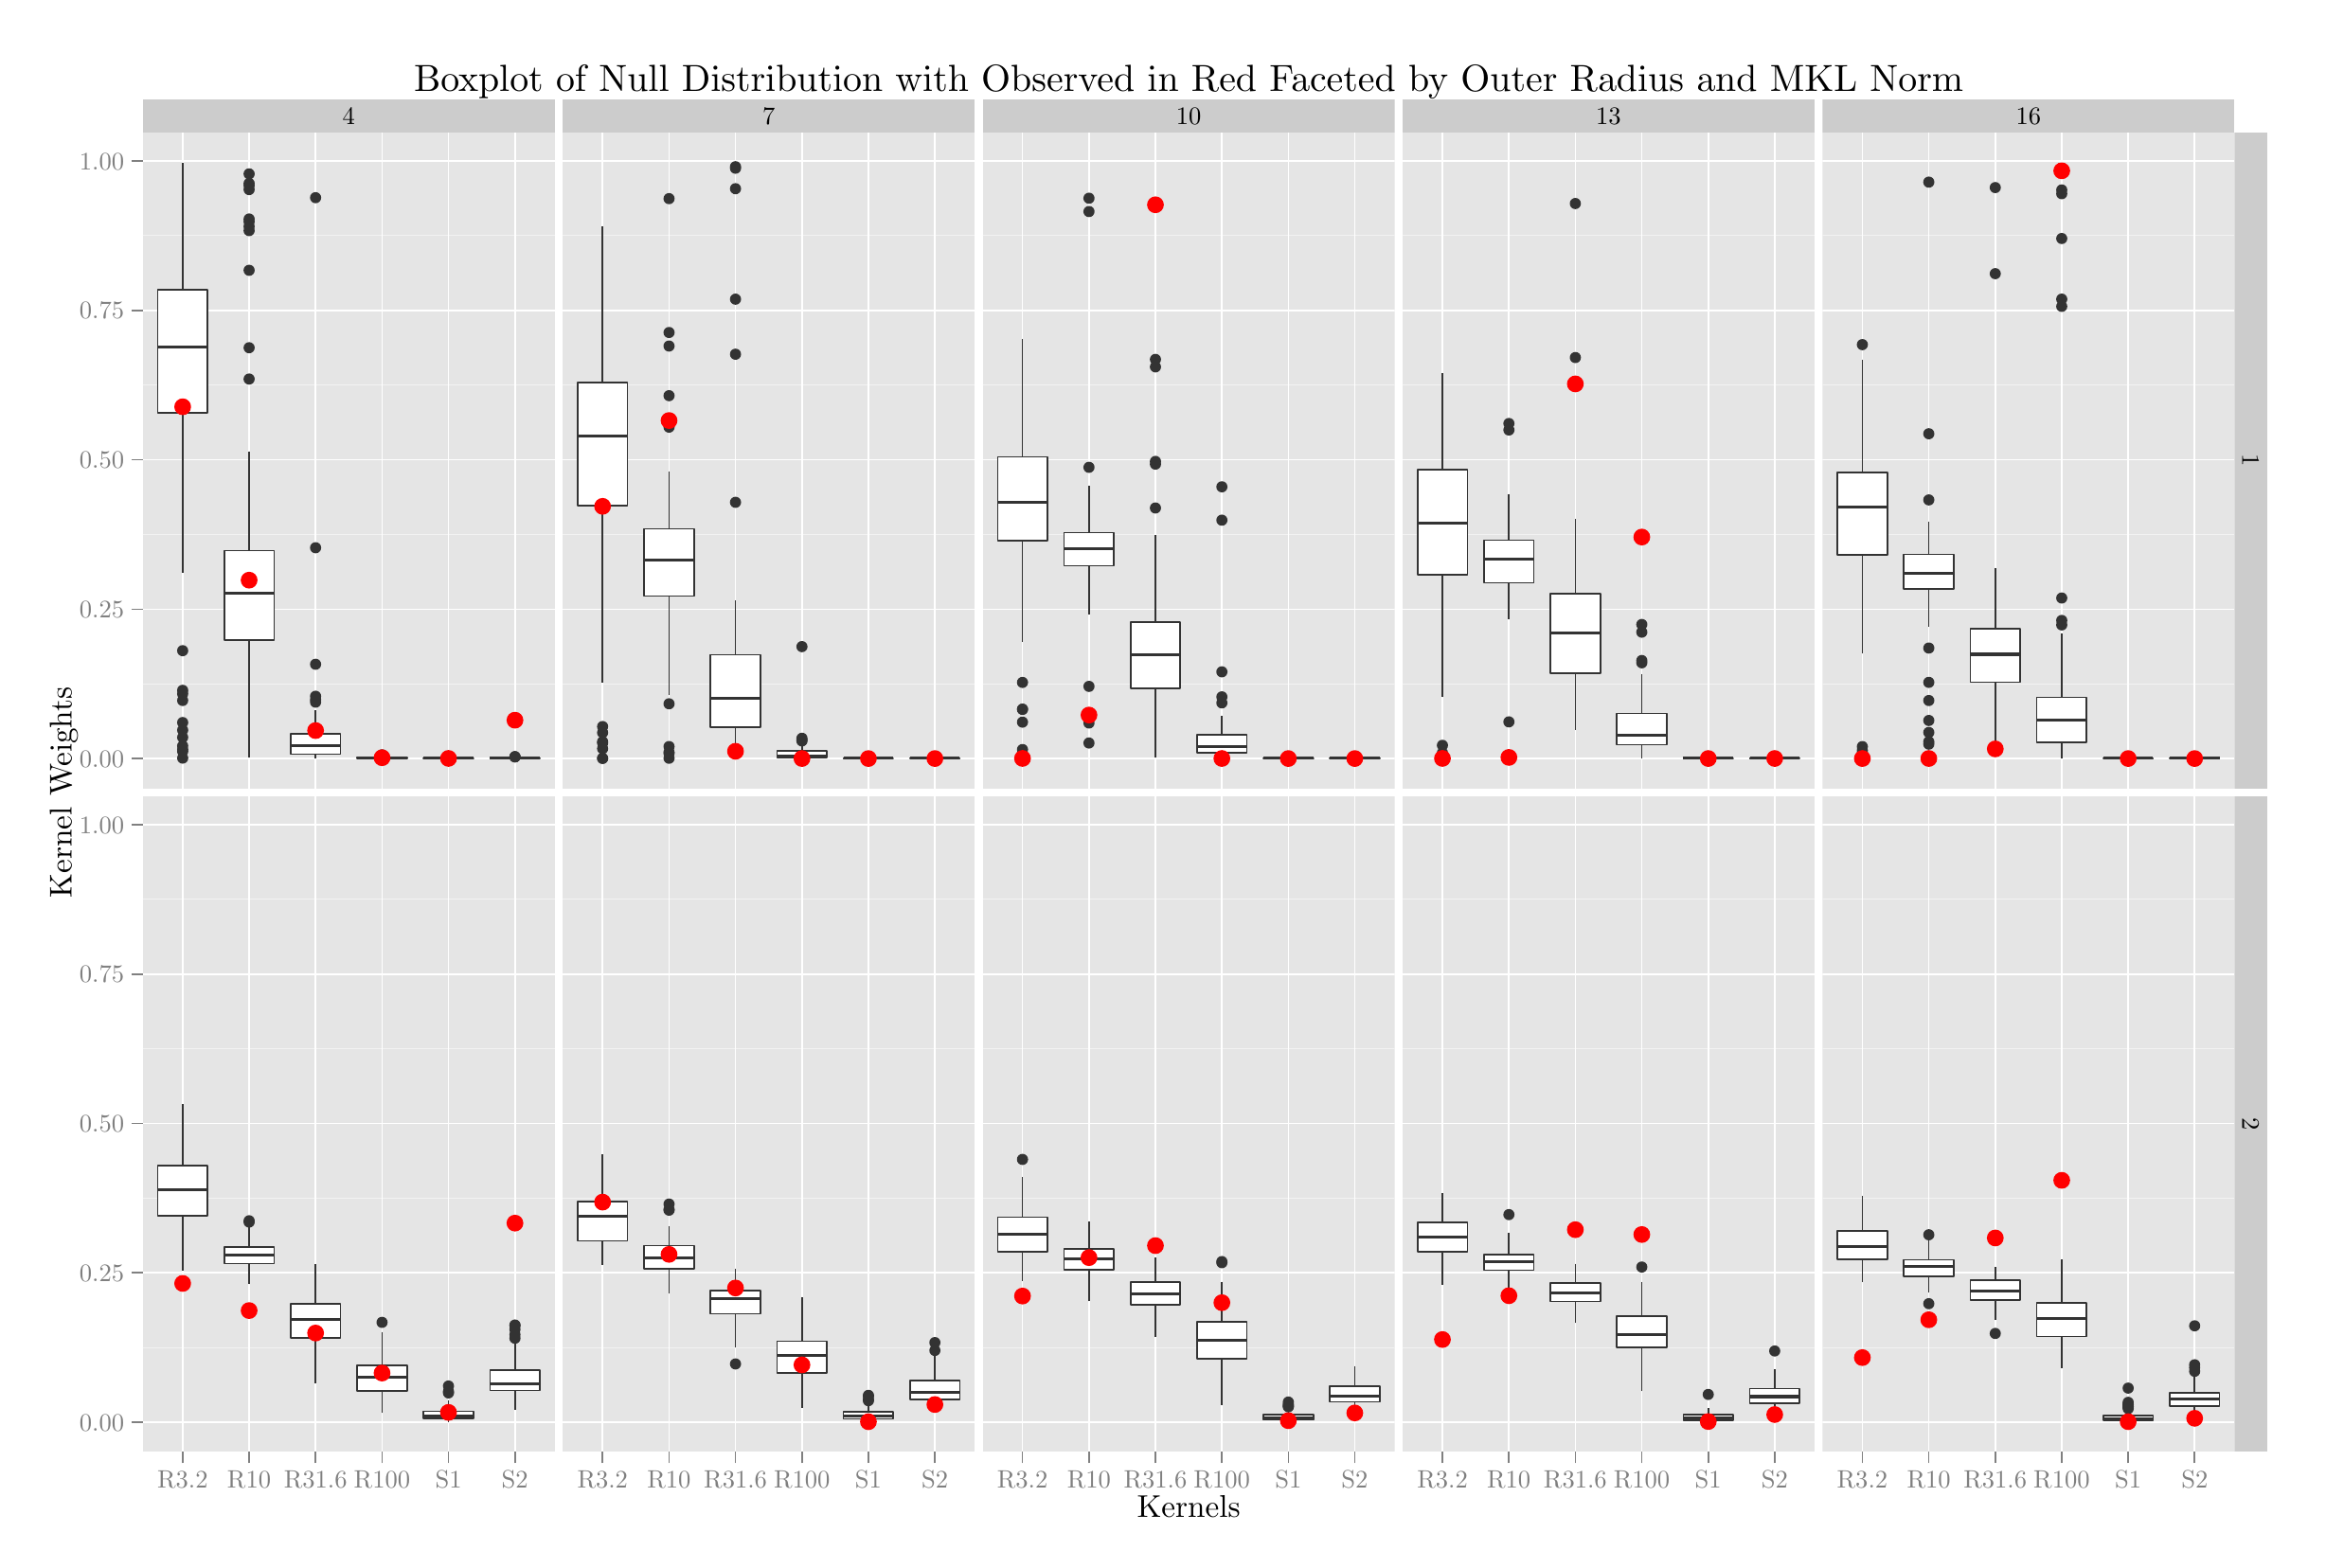
\begin{tikzpicture}[x=1pt,y=1pt]
\definecolor[named]{fillColor}{rgb}{1.00,1.00,1.00}
\path[use as bounding box,fill=fillColor,fill opacity=0.00] (0,0) rectangle (867.24,578.16);
\begin{scope}
\path[clip] (  0.00,  0.00) rectangle (867.24,578.16);
\definecolor[named]{drawColor}{rgb}{1.00,1.00,1.00}
\definecolor[named]{fillColor}{rgb}{1.00,1.00,1.00}

\path[draw=drawColor,line width= 0.6pt,line join=round,line cap=round,fill=fillColor] ( -0.00,  0.00) rectangle (867.24,578.16);
\end{scope}
\begin{scope}
\path[clip] ( 44.49,537.54) rectangle (201.69,550.17);
\definecolor[named]{fillColor}{rgb}{0.80,0.80,0.80}

\path[fill=fillColor] ( 44.49,537.54) rectangle (201.69,550.17);
\definecolor[named]{drawColor}{rgb}{0.00,0.00,0.00}

\node[text=drawColor,anchor=base,inner sep=0pt, outer sep=0pt, scale=  0.96] at (123.09,540.55) {4};
\end{scope}
\begin{scope}
\path[clip] (204.70,537.54) rectangle (361.91,550.17);
\definecolor[named]{fillColor}{rgb}{0.80,0.80,0.80}

\path[fill=fillColor] (204.70,537.54) rectangle (361.91,550.17);
\definecolor[named]{drawColor}{rgb}{0.00,0.00,0.00}

\node[text=drawColor,anchor=base,inner sep=0pt, outer sep=0pt, scale=  0.96] at (283.31,540.55) {7};
\end{scope}
\begin{scope}
\path[clip] (364.92,537.54) rectangle (522.13,550.17);
\definecolor[named]{fillColor}{rgb}{0.80,0.80,0.80}

\path[fill=fillColor] (364.92,537.54) rectangle (522.13,550.17);
\definecolor[named]{drawColor}{rgb}{0.00,0.00,0.00}

\node[text=drawColor,anchor=base,inner sep=0pt, outer sep=0pt, scale=  0.96] at (443.52,540.55) {10};
\end{scope}
\begin{scope}
\path[clip] (525.14,537.54) rectangle (682.34,550.17);
\definecolor[named]{fillColor}{rgb}{0.80,0.80,0.80}

\path[fill=fillColor] (525.14,537.54) rectangle (682.34,550.17);
\definecolor[named]{drawColor}{rgb}{0.00,0.00,0.00}

\node[text=drawColor,anchor=base,inner sep=0pt, outer sep=0pt, scale=  0.96] at (603.74,540.55) {13};
\end{scope}
\begin{scope}
\path[clip] (685.35,537.54) rectangle (842.56,550.17);
\definecolor[named]{fillColor}{rgb}{0.80,0.80,0.80}

\path[fill=fillColor] (685.35,537.54) rectangle (842.56,550.17);
\definecolor[named]{drawColor}{rgb}{0.00,0.00,0.00}

\node[text=drawColor,anchor=base,inner sep=0pt, outer sep=0pt, scale=  0.96] at (763.96,540.55) {16};
\end{scope}
\begin{scope}
\path[clip] ( 44.49,287.29) rectangle (201.69,537.54);
\definecolor[named]{fillColor}{rgb}{0.90,0.90,0.90}

\path[fill=fillColor] ( 44.49,287.29) rectangle (201.69,537.54);
\definecolor[named]{drawColor}{rgb}{0.95,0.95,0.95}

\path[draw=drawColor,line width= 0.3pt,line join=round] ( 44.49,327.17) --
	(201.69,327.17);

\path[draw=drawColor,line width= 0.3pt,line join=round] ( 44.49,384.18) --
	(201.69,384.18);

\path[draw=drawColor,line width= 0.3pt,line join=round] ( 44.49,441.20) --
	(201.69,441.20);

\path[draw=drawColor,line width= 0.3pt,line join=round] ( 44.49,498.21) --
	(201.69,498.21);
\definecolor[named]{drawColor}{rgb}{1.00,1.00,1.00}

\path[draw=drawColor,line width= 0.6pt,line join=round] ( 44.49,298.67) --
	(201.69,298.67);

\path[draw=drawColor,line width= 0.6pt,line join=round] ( 44.49,355.68) --
	(201.69,355.68);

\path[draw=drawColor,line width= 0.6pt,line join=round] ( 44.49,412.69) --
	(201.69,412.69);

\path[draw=drawColor,line width= 0.6pt,line join=round] ( 44.49,469.70) --
	(201.69,469.70);

\path[draw=drawColor,line width= 0.6pt,line join=round] ( 44.49,526.72) --
	(201.69,526.72);

\path[draw=drawColor,line width= 0.6pt,line join=round] ( 59.70,287.29) --
	( 59.70,537.54);

\path[draw=drawColor,line width= 0.6pt,line join=round] ( 85.05,287.29) --
	( 85.05,537.54);

\path[draw=drawColor,line width= 0.6pt,line join=round] (110.41,287.29) --
	(110.41,537.54);

\path[draw=drawColor,line width= 0.6pt,line join=round] (135.77,287.29) --
	(135.77,537.54);

\path[draw=drawColor,line width= 0.6pt,line join=round] (161.12,287.29) --
	(161.12,537.54);

\path[draw=drawColor,line width= 0.6pt,line join=round] (186.48,287.29) --
	(186.48,537.54);
\definecolor[named]{fillColor}{rgb}{0.20,0.20,0.20}

\path[fill=fillColor] ( 59.70,301.39) circle (  2.13);

\path[fill=fillColor] ( 59.70,320.83) circle (  2.13);

\path[fill=fillColor] ( 59.70,309.52) circle (  2.13);

\path[fill=fillColor] ( 59.70,312.41) circle (  2.13);

\path[fill=fillColor] ( 59.70,324.70) circle (  2.13);

\path[fill=fillColor] ( 59.70,303.50) circle (  2.13);

\path[fill=fillColor] ( 59.70,302.12) circle (  2.13);

\path[fill=fillColor] ( 59.70,323.35) circle (  2.13);

\path[fill=fillColor] ( 59.70,339.84) circle (  2.13);

\path[fill=fillColor] ( 59.70,306.75) circle (  2.13);

\path[fill=fillColor] ( 59.70,298.84) circle (  2.13);
\definecolor[named]{drawColor}{rgb}{0.20,0.20,0.20}

\path[draw=drawColor,line width= 0.6pt,line join=round,fill=fillColor] ( 59.70,477.67) -- ( 59.70,526.17);

\path[draw=drawColor,line width= 0.6pt,line join=round,fill=fillColor] ( 59.70,430.69) -- ( 59.70,369.63);
\definecolor[named]{fillColor}{rgb}{1.00,1.00,1.00}

\path[draw=drawColor,line width= 0.6pt,line join=round,line cap=round,fill=fillColor] ( 50.19,477.67) --
	( 50.19,430.69) --
	( 69.21,430.69) --
	( 69.21,477.67) --
	( 50.19,477.67) --
	cycle;
\definecolor[named]{fillColor}{rgb}{0.20,0.20,0.20}

\path[draw=drawColor,line width= 1.1pt,line join=round,fill=fillColor] ( 50.19,455.68) -- ( 69.21,455.68);

\path[fill=fillColor] ( 85.05,443.51) circle (  2.13);

\path[fill=fillColor] ( 85.05,503.57) circle (  2.13);

\path[fill=fillColor] ( 85.05,515.80) circle (  2.13);

\path[fill=fillColor] ( 85.05,504.58) circle (  2.13);

\path[fill=fillColor] ( 85.05,500.14) circle (  2.13);

\path[fill=fillColor] ( 85.05,521.79) circle (  2.13);

\path[fill=fillColor] ( 85.05,517.38) circle (  2.13);

\path[fill=fillColor] ( 85.05,501.71) circle (  2.13);

\path[fill=fillColor] ( 85.05,485.00) circle (  2.13);

\path[fill=fillColor] ( 85.05,518.17) circle (  2.13);

\path[fill=fillColor] ( 85.05,455.45) circle (  2.13);

\path[draw=drawColor,line width= 0.6pt,line join=round,fill=fillColor] ( 85.05,378.02) -- ( 85.05,415.89);

\path[draw=drawColor,line width= 0.6pt,line join=round,fill=fillColor] ( 85.05,343.91) -- ( 85.05,299.20);
\definecolor[named]{fillColor}{rgb}{1.00,1.00,1.00}

\path[draw=drawColor,line width= 0.6pt,line join=round,line cap=round,fill=fillColor] ( 75.55,378.02) --
	( 75.55,343.91) --
	( 94.56,343.91) --
	( 94.56,378.02) --
	( 75.55,378.02) --
	cycle;
\definecolor[named]{fillColor}{rgb}{0.20,0.20,0.20}

\path[draw=drawColor,line width= 1.1pt,line join=round,fill=fillColor] ( 75.55,361.64) -- ( 94.56,361.64);

\path[fill=fillColor] (110.41,320.19) circle (  2.13);

\path[fill=fillColor] (110.41,379.12) circle (  2.13);

\path[fill=fillColor] (110.41,322.45) circle (  2.13);

\path[fill=fillColor] (110.41,321.11) circle (  2.13);

\path[fill=fillColor] (110.41,512.71) circle (  2.13);

\path[fill=fillColor] (110.41,334.65) circle (  2.13);

\path[draw=drawColor,line width= 0.6pt,line join=round,fill=fillColor] (110.41,308.03) -- (110.41,317.12);

\path[draw=drawColor,line width= 0.6pt,line join=round,fill=fillColor] (110.41,300.34) -- (110.41,298.67);
\definecolor[named]{fillColor}{rgb}{1.00,1.00,1.00}

\path[draw=drawColor,line width= 0.6pt,line join=round,line cap=round,fill=fillColor] (100.90,308.03) --
	(100.90,300.34) --
	(119.92,300.34) --
	(119.92,308.03) --
	(100.90,308.03) --
	cycle;
\definecolor[named]{fillColor}{rgb}{0.20,0.20,0.20}

\path[draw=drawColor,line width= 1.1pt,line join=round,fill=fillColor] (100.90,303.42) -- (119.92,303.42);

\path[fill=fillColor] (135.77,299.50) circle (  2.13);

\path[fill=fillColor] (135.77,299.57) circle (  2.13);

\path[fill=fillColor] (135.77,299.61) circle (  2.13);

\path[fill=fillColor] (135.77,299.49) circle (  2.13);

\path[fill=fillColor] (135.77,300.09) circle (  2.13);

\path[draw=drawColor,line width= 0.6pt,line join=round,fill=fillColor] (135.77,299.02) -- (135.77,299.42);

\path[draw=drawColor,line width= 0.6pt,line join=round,fill=fillColor] (135.77,298.75) -- (135.77,298.67);
\definecolor[named]{fillColor}{rgb}{1.00,1.00,1.00}

\path[draw=drawColor,line width= 0.6pt,line join=round,line cap=round,fill=fillColor] (126.26,299.02) --
	(126.26,298.75) --
	(145.27,298.75) --
	(145.27,299.02) --
	(126.26,299.02) --
	cycle;
\definecolor[named]{fillColor}{rgb}{0.20,0.20,0.20}

\path[draw=drawColor,line width= 1.1pt,line join=round,fill=fillColor] (126.26,298.89) -- (145.27,298.89);

\path[fill=fillColor] (161.12,299.03) circle (  2.13);

\path[draw=drawColor,line width= 0.6pt,line join=round,fill=fillColor] (161.12,298.82) -- (161.12,298.97);

\path[draw=drawColor,line width= 0.6pt,line join=round,fill=fillColor] (161.12,298.69) -- (161.12,298.67);
\definecolor[named]{fillColor}{rgb}{1.00,1.00,1.00}

\path[draw=drawColor,line width= 0.6pt,line join=round,line cap=round,fill=fillColor] (151.61,298.82) --
	(151.61,298.69) --
	(170.63,298.69) --
	(170.63,298.82) --
	(151.61,298.82) --
	cycle;
\definecolor[named]{fillColor}{rgb}{0.20,0.20,0.20}

\path[draw=drawColor,line width= 1.1pt,line join=round,fill=fillColor] (151.61,298.75) -- (170.63,298.75);

\path[fill=fillColor] (186.48,299.30) circle (  2.13);

\path[fill=fillColor] (186.48,299.32) circle (  2.13);

\path[fill=fillColor] (186.48,299.41) circle (  2.13);

\path[draw=drawColor,line width= 0.6pt,line join=round,fill=fillColor] (186.48,298.92) -- (186.48,299.24);

\path[draw=drawColor,line width= 0.6pt,line join=round,fill=fillColor] (186.48,298.70) -- (186.48,298.67);
\definecolor[named]{fillColor}{rgb}{1.00,1.00,1.00}

\path[draw=drawColor,line width= 0.6pt,line join=round,line cap=round,fill=fillColor] (176.97,298.92) --
	(176.97,298.70) --
	(195.99,298.70) --
	(195.99,298.92) --
	(176.97,298.92) --
	cycle;
\definecolor[named]{fillColor}{rgb}{0.20,0.20,0.20}

\path[draw=drawColor,line width= 1.1pt,line join=round,fill=fillColor] (176.97,298.83) -- (195.99,298.83);
\definecolor[named]{fillColor}{rgb}{1.00,0.00,0.00}

\path[fill=fillColor] ( 59.70,432.91) circle (  3.20);

\path[fill=fillColor] ( 85.05,366.75) circle (  3.20);

\path[fill=fillColor] (110.41,309.35) circle (  3.20);

\path[fill=fillColor] (135.77,298.99) circle (  3.20);

\path[fill=fillColor] (161.12,298.72) circle (  3.20);

\path[fill=fillColor] (186.48,313.31) circle (  3.20);
\end{scope}
\begin{scope}
\path[clip] ( 44.49, 34.03) rectangle (201.69,284.28);
\definecolor[named]{fillColor}{rgb}{0.90,0.90,0.90}

\path[fill=fillColor] ( 44.49, 34.03) rectangle (201.69,284.28);
\definecolor[named]{drawColor}{rgb}{0.95,0.95,0.95}

\path[draw=drawColor,line width= 0.3pt,line join=round] ( 44.49, 73.91) --
	(201.69, 73.91);

\path[draw=drawColor,line width= 0.3pt,line join=round] ( 44.49,130.93) --
	(201.69,130.93);

\path[draw=drawColor,line width= 0.3pt,line join=round] ( 44.49,187.94) --
	(201.69,187.94);

\path[draw=drawColor,line width= 0.3pt,line join=round] ( 44.49,244.95) --
	(201.69,244.95);
\definecolor[named]{drawColor}{rgb}{1.00,1.00,1.00}

\path[draw=drawColor,line width= 0.6pt,line join=round] ( 44.49, 45.41) --
	(201.69, 45.41);

\path[draw=drawColor,line width= 0.6pt,line join=round] ( 44.49,102.42) --
	(201.69,102.42);

\path[draw=drawColor,line width= 0.6pt,line join=round] ( 44.49,159.43) --
	(201.69,159.43);

\path[draw=drawColor,line width= 0.6pt,line join=round] ( 44.49,216.44) --
	(201.69,216.44);

\path[draw=drawColor,line width= 0.6pt,line join=round] ( 44.49,273.46) --
	(201.69,273.46);

\path[draw=drawColor,line width= 0.6pt,line join=round] ( 59.70, 34.03) --
	( 59.70,284.28);

\path[draw=drawColor,line width= 0.6pt,line join=round] ( 85.05, 34.03) --
	( 85.05,284.28);

\path[draw=drawColor,line width= 0.6pt,line join=round] (110.41, 34.03) --
	(110.41,284.28);

\path[draw=drawColor,line width= 0.6pt,line join=round] (135.77, 34.03) --
	(135.77,284.28);

\path[draw=drawColor,line width= 0.6pt,line join=round] (161.12, 34.03) --
	(161.12,284.28);

\path[draw=drawColor,line width= 0.6pt,line join=round] (186.48, 34.03) --
	(186.48,284.28);
\definecolor[named]{drawColor}{rgb}{0.20,0.20,0.20}
\definecolor[named]{fillColor}{rgb}{0.20,0.20,0.20}

\path[draw=drawColor,line width= 0.6pt,line join=round,fill=fillColor] ( 59.70,143.26) -- ( 59.70,166.78);

\path[draw=drawColor,line width= 0.6pt,line join=round,fill=fillColor] ( 59.70,124.07) -- ( 59.70,103.19);
\definecolor[named]{fillColor}{rgb}{1.00,1.00,1.00}

\path[draw=drawColor,line width= 0.6pt,line join=round,line cap=round,fill=fillColor] ( 50.19,143.26) --
	( 50.19,124.07) --
	( 69.21,124.07) --
	( 69.21,143.26) --
	( 50.19,143.26) --
	cycle;
\definecolor[named]{fillColor}{rgb}{0.20,0.20,0.20}

\path[draw=drawColor,line width= 1.1pt,line join=round,fill=fillColor] ( 50.19,133.95) -- ( 69.21,133.95);

\path[fill=fillColor] ( 85.05,121.78) circle (  2.13);

\path[fill=fillColor] ( 85.05,122.28) circle (  2.13);

\path[draw=drawColor,line width= 0.6pt,line join=round,fill=fillColor] ( 85.05,112.19) -- ( 85.05,121.48);

\path[draw=drawColor,line width= 0.6pt,line join=round,fill=fillColor] ( 85.05,105.96) -- ( 85.05, 97.99);
\definecolor[named]{fillColor}{rgb}{1.00,1.00,1.00}

\path[draw=drawColor,line width= 0.6pt,line join=round,line cap=round,fill=fillColor] ( 75.55,112.19) --
	( 75.55,105.96) --
	( 94.56,105.96) --
	( 94.56,112.19) --
	( 75.55,112.19) --
	cycle;
\definecolor[named]{fillColor}{rgb}{0.20,0.20,0.20}

\path[draw=drawColor,line width= 1.1pt,line join=round,fill=fillColor] ( 75.55,109.29) -- ( 94.56,109.29);

\path[draw=drawColor,line width= 0.6pt,line join=round,fill=fillColor] (110.41, 90.46) -- (110.41,105.75);

\path[draw=drawColor,line width= 0.6pt,line join=round,fill=fillColor] (110.41, 77.48) -- (110.41, 60.37);
\definecolor[named]{fillColor}{rgb}{1.00,1.00,1.00}

\path[draw=drawColor,line width= 0.6pt,line join=round,line cap=round,fill=fillColor] (100.90, 90.46) --
	(100.90, 77.48) --
	(119.92, 77.48) --
	(119.92, 90.46) --
	(100.90, 90.46) --
	cycle;
\definecolor[named]{fillColor}{rgb}{0.20,0.20,0.20}

\path[draw=drawColor,line width= 1.1pt,line join=round,fill=fillColor] (100.90, 84.46) -- (119.92, 84.46);

\path[fill=fillColor] (135.77, 83.50) circle (  2.13);

\path[draw=drawColor,line width= 0.6pt,line join=round,fill=fillColor] (135.77, 67.15) -- (135.77, 79.90);

\path[draw=drawColor,line width= 0.6pt,line join=round,fill=fillColor] (135.77, 57.32) -- (135.77, 48.89);
\definecolor[named]{fillColor}{rgb}{1.00,1.00,1.00}

\path[draw=drawColor,line width= 0.6pt,line join=round,line cap=round,fill=fillColor] (126.26, 67.15) --
	(126.26, 57.32) --
	(145.27, 57.32) --
	(145.27, 67.15) --
	(126.26, 67.15) --
	cycle;
\definecolor[named]{fillColor}{rgb}{0.20,0.20,0.20}

\path[draw=drawColor,line width= 1.1pt,line join=round,fill=fillColor] (126.26, 62.69) -- (145.27, 62.69);

\path[fill=fillColor] (161.12, 59.21) circle (  2.13);

\path[fill=fillColor] (161.12, 56.58) circle (  2.13);

\path[fill=fillColor] (161.12, 57.09) circle (  2.13);

\path[draw=drawColor,line width= 0.6pt,line join=round,fill=fillColor] (161.12, 49.62) -- (161.12, 53.58);

\path[draw=drawColor,line width= 0.6pt,line join=round,fill=fillColor] (161.12, 46.75) -- (161.12, 45.54);
\definecolor[named]{fillColor}{rgb}{1.00,1.00,1.00}

\path[draw=drawColor,line width= 0.6pt,line join=round,line cap=round,fill=fillColor] (151.61, 49.62) --
	(151.61, 46.75) --
	(170.63, 46.75) --
	(170.63, 49.62) --
	(151.61, 49.62) --
	cycle;
\definecolor[named]{fillColor}{rgb}{0.20,0.20,0.20}

\path[draw=drawColor,line width= 1.1pt,line join=round,fill=fillColor] (151.61, 47.93) -- (170.63, 47.93);

\path[fill=fillColor] (186.48, 80.82) circle (  2.13);

\path[fill=fillColor] (186.48, 77.44) circle (  2.13);

\path[fill=fillColor] (186.48, 82.32) circle (  2.13);

\path[fill=fillColor] (186.48, 82.49) circle (  2.13);

\path[fill=fillColor] (186.48, 78.84) circle (  2.13);

\path[draw=drawColor,line width= 0.6pt,line join=round,fill=fillColor] (186.48, 65.40) -- (186.48, 76.86);

\path[draw=drawColor,line width= 0.6pt,line join=round,fill=fillColor] (186.48, 57.52) -- (186.48, 50.20);
\definecolor[named]{fillColor}{rgb}{1.00,1.00,1.00}

\path[draw=drawColor,line width= 0.6pt,line join=round,line cap=round,fill=fillColor] (176.97, 65.40) --
	(176.97, 57.52) --
	(195.99, 57.52) --
	(195.99, 65.40) --
	(176.97, 65.40) --
	cycle;
\definecolor[named]{fillColor}{rgb}{0.20,0.20,0.20}

\path[draw=drawColor,line width= 1.1pt,line join=round,fill=fillColor] (176.97, 59.91) -- (195.99, 59.91);
\definecolor[named]{fillColor}{rgb}{1.00,0.00,0.00}

\path[fill=fillColor] ( 59.70, 98.36) circle (  3.20);

\path[fill=fillColor] ( 85.05, 88.01) circle (  3.20);

\path[fill=fillColor] (110.41, 79.43) circle (  3.20);

\path[fill=fillColor] (135.77, 64.16) circle (  3.20);

\path[fill=fillColor] (161.12, 49.14) circle (  3.20);

\path[fill=fillColor] (186.48,121.38) circle (  3.20);
\end{scope}
\begin{scope}
\path[clip] (204.70,287.29) rectangle (361.91,537.54);
\definecolor[named]{fillColor}{rgb}{0.90,0.90,0.90}

\path[fill=fillColor] (204.70,287.29) rectangle (361.91,537.54);
\definecolor[named]{drawColor}{rgb}{0.95,0.95,0.95}

\path[draw=drawColor,line width= 0.3pt,line join=round] (204.70,327.17) --
	(361.91,327.17);

\path[draw=drawColor,line width= 0.3pt,line join=round] (204.70,384.18) --
	(361.91,384.18);

\path[draw=drawColor,line width= 0.3pt,line join=round] (204.70,441.20) --
	(361.91,441.20);

\path[draw=drawColor,line width= 0.3pt,line join=round] (204.70,498.21) --
	(361.91,498.21);
\definecolor[named]{drawColor}{rgb}{1.00,1.00,1.00}

\path[draw=drawColor,line width= 0.6pt,line join=round] (204.70,298.67) --
	(361.91,298.67);

\path[draw=drawColor,line width= 0.6pt,line join=round] (204.70,355.68) --
	(361.91,355.68);

\path[draw=drawColor,line width= 0.6pt,line join=round] (204.70,412.69) --
	(361.91,412.69);

\path[draw=drawColor,line width= 0.6pt,line join=round] (204.70,469.70) --
	(361.91,469.70);

\path[draw=drawColor,line width= 0.6pt,line join=round] (204.70,526.72) --
	(361.91,526.72);

\path[draw=drawColor,line width= 0.6pt,line join=round] (219.92,287.29) --
	(219.92,537.54);

\path[draw=drawColor,line width= 0.6pt,line join=round] (245.27,287.29) --
	(245.27,537.54);

\path[draw=drawColor,line width= 0.6pt,line join=round] (270.63,287.29) --
	(270.63,537.54);

\path[draw=drawColor,line width= 0.6pt,line join=round] (295.98,287.29) --
	(295.98,537.54);

\path[draw=drawColor,line width= 0.6pt,line join=round] (321.34,287.29) --
	(321.34,537.54);

\path[draw=drawColor,line width= 0.6pt,line join=round] (346.70,287.29) --
	(346.70,537.54);
\definecolor[named]{fillColor}{rgb}{0.20,0.20,0.20}

\path[fill=fillColor] (219.92,310.88) circle (  2.13);

\path[fill=fillColor] (219.92,305.11) circle (  2.13);

\path[fill=fillColor] (219.92,298.74) circle (  2.13);

\path[fill=fillColor] (219.92,302.43) circle (  2.13);

\path[fill=fillColor] (219.92,298.76) circle (  2.13);

\path[fill=fillColor] (219.92,304.61) circle (  2.13);

\path[fill=fillColor] (219.92,308.55) circle (  2.13);
\definecolor[named]{drawColor}{rgb}{0.20,0.20,0.20}

\path[draw=drawColor,line width= 0.6pt,line join=round,fill=fillColor] (219.92,442.18) -- (219.92,501.86);

\path[draw=drawColor,line width= 0.6pt,line join=round,fill=fillColor] (219.92,395.30) -- (219.92,327.80);
\definecolor[named]{fillColor}{rgb}{1.00,1.00,1.00}

\path[draw=drawColor,line width= 0.6pt,line join=round,line cap=round,fill=fillColor] (210.41,442.18) --
	(210.41,395.30) --
	(229.42,395.30) --
	(229.42,442.18) --
	(210.41,442.18) --
	cycle;
\definecolor[named]{fillColor}{rgb}{0.20,0.20,0.20}

\path[draw=drawColor,line width= 1.1pt,line join=round,fill=fillColor] (210.41,421.58) -- (229.42,421.58);

\path[fill=fillColor] (245.27,512.35) circle (  2.13);

\path[fill=fillColor] (245.27,456.09) circle (  2.13);

\path[fill=fillColor] (245.27,437.15) circle (  2.13);

\path[fill=fillColor] (245.27,461.26) circle (  2.13);

\path[fill=fillColor] (245.27,300.63) circle (  2.13);

\path[fill=fillColor] (245.27,425.13) circle (  2.13);

\path[fill=fillColor] (245.27,301.08) circle (  2.13);

\path[fill=fillColor] (245.27,319.57) circle (  2.13);

\path[fill=fillColor] (245.27,303.25) circle (  2.13);

\path[fill=fillColor] (245.27,298.78) circle (  2.13);

\path[draw=drawColor,line width= 0.6pt,line join=round,fill=fillColor] (245.27,386.32) -- (245.27,408.28);

\path[draw=drawColor,line width= 0.6pt,line join=round,fill=fillColor] (245.27,360.73) -- (245.27,322.89);
\definecolor[named]{fillColor}{rgb}{1.00,1.00,1.00}

\path[draw=drawColor,line width= 0.6pt,line join=round,line cap=round,fill=fillColor] (235.76,386.32) --
	(235.76,360.73) --
	(254.78,360.73) --
	(254.78,386.32) --
	(235.76,386.32) --
	cycle;
\definecolor[named]{fillColor}{rgb}{0.20,0.20,0.20}

\path[draw=drawColor,line width= 1.1pt,line join=round,fill=fillColor] (235.76,374.57) -- (254.78,374.57);

\path[fill=fillColor] (270.63,524.53) circle (  2.13);

\path[fill=fillColor] (270.63,396.46) circle (  2.13);

\path[fill=fillColor] (270.63,452.97) circle (  2.13);

\path[fill=fillColor] (270.63,523.95) circle (  2.13);

\path[fill=fillColor] (270.63,516.14) circle (  2.13);

\path[fill=fillColor] (270.63,473.98) circle (  2.13);

\path[draw=drawColor,line width= 0.6pt,line join=round,fill=fillColor] (270.63,338.31) -- (270.63,359.02);

\path[draw=drawColor,line width= 0.6pt,line join=round,fill=fillColor] (270.63,310.55) -- (270.63,298.70);
\definecolor[named]{fillColor}{rgb}{1.00,1.00,1.00}

\path[draw=drawColor,line width= 0.6pt,line join=round,line cap=round,fill=fillColor] (261.12,338.31) --
	(261.12,310.55) --
	(280.14,310.55) --
	(280.14,338.31) --
	(261.12,338.31) --
	cycle;
\definecolor[named]{fillColor}{rgb}{0.20,0.20,0.20}

\path[draw=drawColor,line width= 1.1pt,line join=round,fill=fillColor] (261.12,321.70) -- (280.14,321.70);

\path[fill=fillColor] (295.98,305.39) circle (  2.13);

\path[fill=fillColor] (295.98,306.41) circle (  2.13);

\path[fill=fillColor] (295.98,305.75) circle (  2.13);

\path[fill=fillColor] (295.98,341.38) circle (  2.13);

\path[draw=drawColor,line width= 0.6pt,line join=round,fill=fillColor] (295.98,301.49) -- (295.98,304.49);

\path[draw=drawColor,line width= 0.6pt,line join=round,fill=fillColor] (295.98,299.16) -- (295.98,298.68);
\definecolor[named]{fillColor}{rgb}{1.00,1.00,1.00}

\path[draw=drawColor,line width= 0.6pt,line join=round,line cap=round,fill=fillColor] (286.48,301.49) --
	(286.48,299.16) --
	(305.49,299.16) --
	(305.49,301.49) --
	(286.48,301.49) --
	cycle;
\definecolor[named]{fillColor}{rgb}{0.20,0.20,0.20}

\path[draw=drawColor,line width= 1.1pt,line join=round,fill=fillColor] (286.48,299.63) -- (305.49,299.63);

\path[draw=drawColor,line width= 0.6pt,line join=round,fill=fillColor] (321.34,298.81) -- (321.34,298.89);

\path[draw=drawColor,line width= 0.6pt,line join=round,fill=fillColor] (321.34,298.72) -- (321.34,298.67);
\definecolor[named]{fillColor}{rgb}{1.00,1.00,1.00}

\path[draw=drawColor,line width= 0.6pt,line join=round,line cap=round,fill=fillColor] (311.83,298.81) --
	(311.83,298.72) --
	(330.85,298.72) --
	(330.85,298.81) --
	(311.83,298.81) --
	cycle;
\definecolor[named]{fillColor}{rgb}{0.20,0.20,0.20}

\path[draw=drawColor,line width= 1.1pt,line join=round,fill=fillColor] (311.83,298.77) -- (330.85,298.77);

\path[fill=fillColor] (346.70,299.11) circle (  2.13);

\path[draw=drawColor,line width= 0.6pt,line join=round,fill=fillColor] (346.70,298.89) -- (346.70,299.02);

\path[draw=drawColor,line width= 0.6pt,line join=round,fill=fillColor] (346.70,298.77) -- (346.70,298.67);
\definecolor[named]{fillColor}{rgb}{1.00,1.00,1.00}

\path[draw=drawColor,line width= 0.6pt,line join=round,line cap=round,fill=fillColor] (337.19,298.89) --
	(337.19,298.77) --
	(356.20,298.77) --
	(356.20,298.89) --
	(337.19,298.89) --
	cycle;
\definecolor[named]{fillColor}{rgb}{0.20,0.20,0.20}

\path[draw=drawColor,line width= 1.1pt,line join=round,fill=fillColor] (337.19,298.84) -- (356.20,298.84);
\definecolor[named]{fillColor}{rgb}{1.00,0.00,0.00}

\path[fill=fillColor] (219.92,394.92) circle (  3.20);

\path[fill=fillColor] (245.27,427.67) circle (  3.20);

\path[fill=fillColor] (270.63,301.44) circle (  3.20);

\path[fill=fillColor] (295.98,298.68) circle (  3.20);

\path[fill=fillColor] (321.34,298.67) circle (  3.20);

\path[fill=fillColor] (346.70,298.67) circle (  3.20);
\end{scope}
\begin{scope}
\path[clip] (204.70, 34.03) rectangle (361.91,284.28);
\definecolor[named]{fillColor}{rgb}{0.90,0.90,0.90}

\path[fill=fillColor] (204.70, 34.03) rectangle (361.91,284.28);
\definecolor[named]{drawColor}{rgb}{0.95,0.95,0.95}

\path[draw=drawColor,line width= 0.3pt,line join=round] (204.70, 73.91) --
	(361.91, 73.91);

\path[draw=drawColor,line width= 0.3pt,line join=round] (204.70,130.93) --
	(361.91,130.93);

\path[draw=drawColor,line width= 0.3pt,line join=round] (204.70,187.94) --
	(361.91,187.94);

\path[draw=drawColor,line width= 0.3pt,line join=round] (204.70,244.95) --
	(361.91,244.95);
\definecolor[named]{drawColor}{rgb}{1.00,1.00,1.00}

\path[draw=drawColor,line width= 0.6pt,line join=round] (204.70, 45.41) --
	(361.91, 45.41);

\path[draw=drawColor,line width= 0.6pt,line join=round] (204.70,102.42) --
	(361.91,102.42);

\path[draw=drawColor,line width= 0.6pt,line join=round] (204.70,159.43) --
	(361.91,159.43);

\path[draw=drawColor,line width= 0.6pt,line join=round] (204.70,216.44) --
	(361.91,216.44);

\path[draw=drawColor,line width= 0.6pt,line join=round] (204.70,273.46) --
	(361.91,273.46);

\path[draw=drawColor,line width= 0.6pt,line join=round] (219.92, 34.03) --
	(219.92,284.28);

\path[draw=drawColor,line width= 0.6pt,line join=round] (245.27, 34.03) --
	(245.27,284.28);

\path[draw=drawColor,line width= 0.6pt,line join=round] (270.63, 34.03) --
	(270.63,284.28);

\path[draw=drawColor,line width= 0.6pt,line join=round] (295.98, 34.03) --
	(295.98,284.28);

\path[draw=drawColor,line width= 0.6pt,line join=round] (321.34, 34.03) --
	(321.34,284.28);

\path[draw=drawColor,line width= 0.6pt,line join=round] (346.70, 34.03) --
	(346.70,284.28);
\definecolor[named]{drawColor}{rgb}{0.20,0.20,0.20}
\definecolor[named]{fillColor}{rgb}{0.20,0.20,0.20}

\path[draw=drawColor,line width= 0.6pt,line join=round,fill=fillColor] (219.92,129.62) -- (219.92,147.65);

\path[draw=drawColor,line width= 0.6pt,line join=round,fill=fillColor] (219.92,114.63) -- (219.92,105.55);
\definecolor[named]{fillColor}{rgb}{1.00,1.00,1.00}

\path[draw=drawColor,line width= 0.6pt,line join=round,line cap=round,fill=fillColor] (210.41,129.62) --
	(210.41,114.63) --
	(229.42,114.63) --
	(229.42,129.62) --
	(210.41,129.62) --
	cycle;
\definecolor[named]{fillColor}{rgb}{0.20,0.20,0.20}

\path[draw=drawColor,line width= 1.1pt,line join=round,fill=fillColor] (210.41,124.05) -- (229.42,124.05);

\path[fill=fillColor] (245.27,128.65) circle (  2.13);

\path[fill=fillColor] (245.27,126.31) circle (  2.13);

\path[fill=fillColor] (245.27,126.56) circle (  2.13);

\path[draw=drawColor,line width= 0.6pt,line join=round,fill=fillColor] (245.27,112.84) -- (245.27,120.26);

\path[draw=drawColor,line width= 0.6pt,line join=round,fill=fillColor] (245.27,104.02) -- (245.27, 94.45);
\definecolor[named]{fillColor}{rgb}{1.00,1.00,1.00}

\path[draw=drawColor,line width= 0.6pt,line join=round,line cap=round,fill=fillColor] (235.76,112.84) --
	(235.76,104.02) --
	(254.78,104.02) --
	(254.78,112.84) --
	(235.76,112.84) --
	cycle;
\definecolor[named]{fillColor}{rgb}{0.20,0.20,0.20}

\path[draw=drawColor,line width= 1.1pt,line join=round,fill=fillColor] (235.76,108.24) -- (254.78,108.24);

\path[fill=fillColor] (270.63, 67.64) circle (  2.13);

\path[draw=drawColor,line width= 0.6pt,line join=round,fill=fillColor] (270.63, 95.56) -- (270.63,103.93);

\path[draw=drawColor,line width= 0.6pt,line join=round,fill=fillColor] (270.63, 86.79) -- (270.63, 73.82);
\definecolor[named]{fillColor}{rgb}{1.00,1.00,1.00}

\path[draw=drawColor,line width= 0.6pt,line join=round,line cap=round,fill=fillColor] (261.12, 95.56) --
	(261.12, 86.79) --
	(280.14, 86.79) --
	(280.14, 95.56) --
	(261.12, 95.56) --
	cycle;
\definecolor[named]{fillColor}{rgb}{0.20,0.20,0.20}

\path[draw=drawColor,line width= 1.1pt,line join=round,fill=fillColor] (261.12, 92.55) -- (280.14, 92.55);

\path[draw=drawColor,line width= 0.6pt,line join=round,fill=fillColor] (295.98, 76.27) -- (295.98, 93.15);

\path[draw=drawColor,line width= 0.6pt,line join=round,fill=fillColor] (295.98, 64.23) -- (295.98, 50.99);
\definecolor[named]{fillColor}{rgb}{1.00,1.00,1.00}

\path[draw=drawColor,line width= 0.6pt,line join=round,line cap=round,fill=fillColor] (286.48, 76.27) --
	(286.48, 64.23) --
	(305.49, 64.23) --
	(305.49, 76.27) --
	(286.48, 76.27) --
	cycle;
\definecolor[named]{fillColor}{rgb}{0.20,0.20,0.20}

\path[draw=drawColor,line width= 1.1pt,line join=round,fill=fillColor] (286.48, 70.75) -- (305.49, 70.75);

\path[fill=fillColor] (321.34, 55.65) circle (  2.13);

\path[fill=fillColor] (321.34, 54.04) circle (  2.13);

\path[fill=fillColor] (321.34, 53.61) circle (  2.13);

\path[fill=fillColor] (321.34, 55.33) circle (  2.13);

\path[draw=drawColor,line width= 0.6pt,line join=round,fill=fillColor] (321.34, 49.42) -- (321.34, 52.88);

\path[draw=drawColor,line width= 0.6pt,line join=round,fill=fillColor] (321.34, 46.68) -- (321.34, 45.44);
\definecolor[named]{fillColor}{rgb}{1.00,1.00,1.00}

\path[draw=drawColor,line width= 0.6pt,line join=round,line cap=round,fill=fillColor] (311.83, 49.42) --
	(311.83, 46.68) --
	(330.85, 46.68) --
	(330.85, 49.42) --
	(311.83, 49.42) --
	cycle;
\definecolor[named]{fillColor}{rgb}{0.20,0.20,0.20}

\path[draw=drawColor,line width= 1.1pt,line join=round,fill=fillColor] (311.83, 47.72) -- (330.85, 47.72);

\path[fill=fillColor] (346.70, 75.79) circle (  2.13);

\path[fill=fillColor] (346.70, 72.78) circle (  2.13);

\path[draw=drawColor,line width= 0.6pt,line join=round,fill=fillColor] (346.70, 61.33) -- (346.70, 71.75);

\path[draw=drawColor,line width= 0.6pt,line join=round,fill=fillColor] (346.70, 54.11) -- (346.70, 50.73);
\definecolor[named]{fillColor}{rgb}{1.00,1.00,1.00}

\path[draw=drawColor,line width= 0.6pt,line join=round,line cap=round,fill=fillColor] (337.19, 61.33) --
	(337.19, 54.11) --
	(356.20, 54.11) --
	(356.20, 61.33) --
	(337.19, 61.33) --
	cycle;
\definecolor[named]{fillColor}{rgb}{0.20,0.20,0.20}

\path[draw=drawColor,line width= 1.1pt,line join=round,fill=fillColor] (337.19, 56.88) -- (356.20, 56.88);
\definecolor[named]{fillColor}{rgb}{1.00,0.00,0.00}

\path[fill=fillColor] (219.92,129.40) circle (  3.20);

\path[fill=fillColor] (245.27,109.45) circle (  3.20);

\path[fill=fillColor] (270.63, 96.62) circle (  3.20);

\path[fill=fillColor] (295.98, 67.28) circle (  3.20);

\path[fill=fillColor] (321.34, 45.59) circle (  3.20);

\path[fill=fillColor] (346.70, 52.15) circle (  3.20);
\end{scope}
\begin{scope}
\path[clip] (364.92,287.29) rectangle (522.13,537.54);
\definecolor[named]{fillColor}{rgb}{0.90,0.90,0.90}

\path[fill=fillColor] (364.92,287.29) rectangle (522.13,537.54);
\definecolor[named]{drawColor}{rgb}{0.95,0.95,0.95}

\path[draw=drawColor,line width= 0.3pt,line join=round] (364.92,327.17) --
	(522.13,327.17);

\path[draw=drawColor,line width= 0.3pt,line join=round] (364.92,384.18) --
	(522.13,384.18);

\path[draw=drawColor,line width= 0.3pt,line join=round] (364.92,441.20) --
	(522.13,441.20);

\path[draw=drawColor,line width= 0.3pt,line join=round] (364.92,498.21) --
	(522.13,498.21);
\definecolor[named]{drawColor}{rgb}{1.00,1.00,1.00}

\path[draw=drawColor,line width= 0.6pt,line join=round] (364.92,298.67) --
	(522.13,298.67);

\path[draw=drawColor,line width= 0.6pt,line join=round] (364.92,355.68) --
	(522.13,355.68);

\path[draw=drawColor,line width= 0.6pt,line join=round] (364.92,412.69) --
	(522.13,412.69);

\path[draw=drawColor,line width= 0.6pt,line join=round] (364.92,469.70) --
	(522.13,469.70);

\path[draw=drawColor,line width= 0.6pt,line join=round] (364.92,526.72) --
	(522.13,526.72);

\path[draw=drawColor,line width= 0.6pt,line join=round] (380.13,287.29) --
	(380.13,537.54);

\path[draw=drawColor,line width= 0.6pt,line join=round] (405.49,287.29) --
	(405.49,537.54);

\path[draw=drawColor,line width= 0.6pt,line join=round] (430.85,287.29) --
	(430.85,537.54);

\path[draw=drawColor,line width= 0.6pt,line join=round] (456.20,287.29) --
	(456.20,537.54);

\path[draw=drawColor,line width= 0.6pt,line join=round] (481.56,287.29) --
	(481.56,537.54);

\path[draw=drawColor,line width= 0.6pt,line join=round] (506.91,287.29) --
	(506.91,537.54);
\definecolor[named]{fillColor}{rgb}{0.20,0.20,0.20}

\path[fill=fillColor] (380.13,312.56) circle (  2.13);

\path[fill=fillColor] (380.13,317.53) circle (  2.13);

\path[fill=fillColor] (380.13,299.78) circle (  2.13);

\path[fill=fillColor] (380.13,317.43) circle (  2.13);

\path[fill=fillColor] (380.13,299.84) circle (  2.13);

\path[fill=fillColor] (380.13,327.72) circle (  2.13);

\path[fill=fillColor] (380.13,302.10) circle (  2.13);
\definecolor[named]{drawColor}{rgb}{0.20,0.20,0.20}

\path[draw=drawColor,line width= 0.6pt,line join=round,fill=fillColor] (380.13,413.78) -- (380.13,458.80);

\path[draw=drawColor,line width= 0.6pt,line join=round,fill=fillColor] (380.13,381.86) -- (380.13,343.15);
\definecolor[named]{fillColor}{rgb}{1.00,1.00,1.00}

\path[draw=drawColor,line width= 0.6pt,line join=round,line cap=round,fill=fillColor] (370.63,413.78) --
	(370.63,381.86) --
	(389.64,381.86) --
	(389.64,413.78) --
	(370.63,413.78) --
	cycle;
\definecolor[named]{fillColor}{rgb}{0.20,0.20,0.20}

\path[draw=drawColor,line width= 1.1pt,line join=round,fill=fillColor] (370.63,396.55) -- (389.64,396.55);

\path[fill=fillColor] (405.49,512.51) circle (  2.13);

\path[fill=fillColor] (405.49,507.42) circle (  2.13);

\path[fill=fillColor] (405.49,304.60) circle (  2.13);

\path[fill=fillColor] (405.49,326.21) circle (  2.13);

\path[fill=fillColor] (405.49,312.23) circle (  2.13);

\path[fill=fillColor] (405.49,409.81) circle (  2.13);

\path[draw=drawColor,line width= 0.6pt,line join=round,fill=fillColor] (405.49,384.91) -- (405.49,402.82);

\path[draw=drawColor,line width= 0.6pt,line join=round,fill=fillColor] (405.49,372.25) -- (405.49,353.63);
\definecolor[named]{fillColor}{rgb}{1.00,1.00,1.00}

\path[draw=drawColor,line width= 0.6pt,line join=round,line cap=round,fill=fillColor] (395.98,384.91) --
	(395.98,372.25) --
	(415.00,372.25) --
	(415.00,384.91) --
	(395.98,384.91) --
	cycle;
\definecolor[named]{fillColor}{rgb}{0.20,0.20,0.20}

\path[draw=drawColor,line width= 1.1pt,line join=round,fill=fillColor] (395.98,378.69) -- (415.00,378.69);

\path[fill=fillColor] (430.85,448.14) circle (  2.13);

\path[fill=fillColor] (430.85,411.03) circle (  2.13);

\path[fill=fillColor] (430.85,394.29) circle (  2.13);

\path[fill=fillColor] (430.85,450.99) circle (  2.13);

\path[fill=fillColor] (430.85,412.07) circle (  2.13);

\path[draw=drawColor,line width= 0.6pt,line join=round,fill=fillColor] (430.85,350.84) -- (430.85,383.84);

\path[draw=drawColor,line width= 0.6pt,line join=round,fill=fillColor] (430.85,325.39) -- (430.85,298.93);
\definecolor[named]{fillColor}{rgb}{1.00,1.00,1.00}

\path[draw=drawColor,line width= 0.6pt,line join=round,line cap=round,fill=fillColor] (421.34,350.84) --
	(421.34,325.39) --
	(440.35,325.39) --
	(440.35,350.84) --
	(421.34,350.84) --
	cycle;
\definecolor[named]{fillColor}{rgb}{0.20,0.20,0.20}

\path[draw=drawColor,line width= 1.1pt,line join=round,fill=fillColor] (421.34,338.24) -- (440.35,338.24);

\path[fill=fillColor] (456.20,322.21) circle (  2.13);

\path[fill=fillColor] (456.20,389.65) circle (  2.13);

\path[fill=fillColor] (456.20,402.37) circle (  2.13);

\path[fill=fillColor] (456.20,331.76) circle (  2.13);

\path[fill=fillColor] (456.20,319.91) circle (  2.13);

\path[draw=drawColor,line width= 0.6pt,line join=round,fill=fillColor] (456.20,307.64) -- (456.20,315.06);

\path[draw=drawColor,line width= 0.6pt,line join=round,fill=fillColor] (456.20,301.00) -- (456.20,298.69);
\definecolor[named]{fillColor}{rgb}{1.00,1.00,1.00}

\path[draw=drawColor,line width= 0.6pt,line join=round,line cap=round,fill=fillColor] (446.69,307.64) --
	(446.69,301.00) --
	(465.71,301.00) --
	(465.71,307.64) --
	(446.69,307.64) --
	cycle;
\definecolor[named]{fillColor}{rgb}{0.20,0.20,0.20}

\path[draw=drawColor,line width= 1.1pt,line join=round,fill=fillColor] (446.69,303.09) -- (465.71,303.09);

\path[draw=drawColor,line width= 0.6pt,line join=round,fill=fillColor] (481.56,298.78) -- (481.56,298.87);

\path[draw=drawColor,line width= 0.6pt,line join=round,fill=fillColor] (481.56,298.71) -- (481.56,298.67);
\definecolor[named]{fillColor}{rgb}{1.00,1.00,1.00}

\path[draw=drawColor,line width= 0.6pt,line join=round,line cap=round,fill=fillColor] (472.05,298.78) --
	(472.05,298.71) --
	(491.07,298.71) --
	(491.07,298.78) --
	(472.05,298.78) --
	cycle;
\definecolor[named]{fillColor}{rgb}{0.20,0.20,0.20}

\path[draw=drawColor,line width= 1.1pt,line join=round,fill=fillColor] (472.05,298.74) -- (491.07,298.74);

\path[draw=drawColor,line width= 0.6pt,line join=round,fill=fillColor] (506.91,298.84) -- (506.91,298.97);

\path[draw=drawColor,line width= 0.6pt,line join=round,fill=fillColor] (506.91,298.74) -- (506.91,298.67);
\definecolor[named]{fillColor}{rgb}{1.00,1.00,1.00}

\path[draw=drawColor,line width= 0.6pt,line join=round,line cap=round,fill=fillColor] (497.40,298.84) --
	(497.40,298.74) --
	(516.42,298.74) --
	(516.42,298.84) --
	(497.40,298.84) --
	cycle;
\definecolor[named]{fillColor}{rgb}{0.20,0.20,0.20}

\path[draw=drawColor,line width= 1.1pt,line join=round,fill=fillColor] (497.40,298.80) -- (516.42,298.80);
\definecolor[named]{fillColor}{rgb}{1.00,0.00,0.00}

\path[fill=fillColor] (380.13,298.72) circle (  3.20);

\path[fill=fillColor] (405.49,315.27) circle (  3.20);

\path[fill=fillColor] (430.85,510.00) circle (  3.20);

\path[fill=fillColor] (456.20,298.70) circle (  3.20);

\path[fill=fillColor] (481.56,298.67) circle (  3.20);

\path[fill=fillColor] (506.91,298.67) circle (  3.20);
\end{scope}
\begin{scope}
\path[clip] (364.92, 34.03) rectangle (522.13,284.28);
\definecolor[named]{fillColor}{rgb}{0.90,0.90,0.90}

\path[fill=fillColor] (364.92, 34.03) rectangle (522.13,284.28);
\definecolor[named]{drawColor}{rgb}{0.95,0.95,0.95}

\path[draw=drawColor,line width= 0.3pt,line join=round] (364.92, 73.91) --
	(522.13, 73.91);

\path[draw=drawColor,line width= 0.3pt,line join=round] (364.92,130.93) --
	(522.13,130.93);

\path[draw=drawColor,line width= 0.3pt,line join=round] (364.92,187.94) --
	(522.13,187.94);

\path[draw=drawColor,line width= 0.3pt,line join=round] (364.92,244.95) --
	(522.13,244.95);
\definecolor[named]{drawColor}{rgb}{1.00,1.00,1.00}

\path[draw=drawColor,line width= 0.6pt,line join=round] (364.92, 45.41) --
	(522.13, 45.41);

\path[draw=drawColor,line width= 0.6pt,line join=round] (364.92,102.42) --
	(522.13,102.42);

\path[draw=drawColor,line width= 0.6pt,line join=round] (364.92,159.43) --
	(522.13,159.43);

\path[draw=drawColor,line width= 0.6pt,line join=round] (364.92,216.44) --
	(522.13,216.44);

\path[draw=drawColor,line width= 0.6pt,line join=round] (364.92,273.46) --
	(522.13,273.46);

\path[draw=drawColor,line width= 0.6pt,line join=round] (380.13, 34.03) --
	(380.13,284.28);

\path[draw=drawColor,line width= 0.6pt,line join=round] (405.49, 34.03) --
	(405.49,284.28);

\path[draw=drawColor,line width= 0.6pt,line join=round] (430.85, 34.03) --
	(430.85,284.28);

\path[draw=drawColor,line width= 0.6pt,line join=round] (456.20, 34.03) --
	(456.20,284.28);

\path[draw=drawColor,line width= 0.6pt,line join=round] (481.56, 34.03) --
	(481.56,284.28);

\path[draw=drawColor,line width= 0.6pt,line join=round] (506.91, 34.03) --
	(506.91,284.28);
\definecolor[named]{fillColor}{rgb}{0.20,0.20,0.20}

\path[fill=fillColor] (380.13,145.69) circle (  2.13);
\definecolor[named]{drawColor}{rgb}{0.20,0.20,0.20}

\path[draw=drawColor,line width= 0.6pt,line join=round,fill=fillColor] (380.13,123.62) -- (380.13,138.96);

\path[draw=drawColor,line width= 0.6pt,line join=round,fill=fillColor] (380.13,110.35) -- (380.13, 99.34);
\definecolor[named]{fillColor}{rgb}{1.00,1.00,1.00}

\path[draw=drawColor,line width= 0.6pt,line join=round,line cap=round,fill=fillColor] (370.63,123.62) --
	(370.63,110.35) --
	(389.64,110.35) --
	(389.64,123.62) --
	(370.63,123.62) --
	cycle;
\definecolor[named]{fillColor}{rgb}{0.20,0.20,0.20}

\path[draw=drawColor,line width= 1.1pt,line join=round,fill=fillColor] (370.63,117.07) -- (389.64,117.07);

\path[draw=drawColor,line width= 0.6pt,line join=round,fill=fillColor] (405.49,111.58) -- (405.49,121.90);

\path[draw=drawColor,line width= 0.6pt,line join=round,fill=fillColor] (405.49,103.51) -- (405.49, 91.56);
\definecolor[named]{fillColor}{rgb}{1.00,1.00,1.00}

\path[draw=drawColor,line width= 0.6pt,line join=round,line cap=round,fill=fillColor] (395.98,111.58) --
	(395.98,103.51) --
	(415.00,103.51) --
	(415.00,111.58) --
	(395.98,111.58) --
	cycle;
\definecolor[named]{fillColor}{rgb}{0.20,0.20,0.20}

\path[draw=drawColor,line width= 1.1pt,line join=round,fill=fillColor] (395.98,107.71) -- (415.00,107.71);

\path[draw=drawColor,line width= 0.6pt,line join=round,fill=fillColor] (430.85, 98.83) -- (430.85,108.28);

\path[draw=drawColor,line width= 0.6pt,line join=round,fill=fillColor] (430.85, 90.29) -- (430.85, 78.10);
\definecolor[named]{fillColor}{rgb}{1.00,1.00,1.00}

\path[draw=drawColor,line width= 0.6pt,line join=round,line cap=round,fill=fillColor] (421.34, 98.83) --
	(421.34, 90.29) --
	(440.35, 90.29) --
	(440.35, 98.83) --
	(421.34, 98.83) --
	cycle;
\definecolor[named]{fillColor}{rgb}{0.20,0.20,0.20}

\path[draw=drawColor,line width= 1.1pt,line join=round,fill=fillColor] (421.34, 94.48) -- (440.35, 94.48);

\path[fill=fillColor] (456.20,106.71) circle (  2.13);

\path[fill=fillColor] (456.20,106.27) circle (  2.13);

\path[draw=drawColor,line width= 0.6pt,line join=round,fill=fillColor] (456.20, 83.75) -- (456.20, 99.07);

\path[draw=drawColor,line width= 0.6pt,line join=round,fill=fillColor] (456.20, 69.72) -- (456.20, 51.86);
\definecolor[named]{fillColor}{rgb}{1.00,1.00,1.00}

\path[draw=drawColor,line width= 0.6pt,line join=round,line cap=round,fill=fillColor] (446.69, 83.75) --
	(446.69, 69.72) --
	(465.71, 69.72) --
	(465.71, 83.75) --
	(446.69, 83.75) --
	cycle;
\definecolor[named]{fillColor}{rgb}{0.20,0.20,0.20}

\path[draw=drawColor,line width= 1.1pt,line join=round,fill=fillColor] (446.69, 76.78) -- (465.71, 76.78);

\path[fill=fillColor] (481.56, 51.84) circle (  2.13);

\path[fill=fillColor] (481.56, 52.27) circle (  2.13);

\path[fill=fillColor] (481.56, 51.47) circle (  2.13);

\path[fill=fillColor] (481.56, 51.27) circle (  2.13);

\path[fill=fillColor] (481.56, 53.09) circle (  2.13);

\path[draw=drawColor,line width= 0.6pt,line join=round,fill=fillColor] (481.56, 48.28) -- (481.56, 51.13);

\path[draw=drawColor,line width= 0.6pt,line join=round,fill=fillColor] (481.56, 46.33) -- (481.56, 45.51);
\definecolor[named]{fillColor}{rgb}{1.00,1.00,1.00}

\path[draw=drawColor,line width= 0.6pt,line join=round,line cap=round,fill=fillColor] (472.05, 48.28) --
	(472.05, 46.33) --
	(491.07, 46.33) --
	(491.07, 48.28) --
	(472.05, 48.28) --
	cycle;
\definecolor[named]{fillColor}{rgb}{0.20,0.20,0.20}

\path[draw=drawColor,line width= 1.1pt,line join=round,fill=fillColor] (472.05, 47.11) -- (491.07, 47.11);

\path[draw=drawColor,line width= 0.6pt,line join=round,fill=fillColor] (506.91, 59.17) -- (506.91, 66.89);

\path[draw=drawColor,line width= 0.6pt,line join=round,fill=fillColor] (506.91, 53.13) -- (506.91, 48.59);
\definecolor[named]{fillColor}{rgb}{1.00,1.00,1.00}

\path[draw=drawColor,line width= 0.6pt,line join=round,line cap=round,fill=fillColor] (497.40, 59.17) --
	(497.40, 53.13) --
	(516.42, 53.13) --
	(516.42, 59.17) --
	(497.40, 59.17) --
	cycle;
\definecolor[named]{fillColor}{rgb}{0.20,0.20,0.20}

\path[draw=drawColor,line width= 1.1pt,line join=round,fill=fillColor] (497.40, 55.47) -- (516.42, 55.47);
\definecolor[named]{fillColor}{rgb}{1.00,0.00,0.00}

\path[fill=fillColor] (380.13, 93.55) circle (  3.20);

\path[fill=fillColor] (405.49,108.21) circle (  3.20);

\path[fill=fillColor] (430.85,112.79) circle (  3.20);

\path[fill=fillColor] (456.20, 91.01) circle (  3.20);

\path[fill=fillColor] (481.56, 45.99) circle (  3.20);

\path[fill=fillColor] (506.91, 48.94) circle (  3.20);
\end{scope}
\begin{scope}
\path[clip] (525.14,287.29) rectangle (682.34,537.54);
\definecolor[named]{fillColor}{rgb}{0.90,0.90,0.90}

\path[fill=fillColor] (525.14,287.29) rectangle (682.34,537.54);
\definecolor[named]{drawColor}{rgb}{0.95,0.95,0.95}

\path[draw=drawColor,line width= 0.3pt,line join=round] (525.14,327.17) --
	(682.34,327.17);

\path[draw=drawColor,line width= 0.3pt,line join=round] (525.14,384.18) --
	(682.34,384.18);

\path[draw=drawColor,line width= 0.3pt,line join=round] (525.14,441.20) --
	(682.34,441.20);

\path[draw=drawColor,line width= 0.3pt,line join=round] (525.14,498.21) --
	(682.34,498.21);
\definecolor[named]{drawColor}{rgb}{1.00,1.00,1.00}

\path[draw=drawColor,line width= 0.6pt,line join=round] (525.14,298.67) --
	(682.34,298.67);

\path[draw=drawColor,line width= 0.6pt,line join=round] (525.14,355.68) --
	(682.34,355.68);

\path[draw=drawColor,line width= 0.6pt,line join=round] (525.14,412.69) --
	(682.34,412.69);

\path[draw=drawColor,line width= 0.6pt,line join=round] (525.14,469.70) --
	(682.34,469.70);

\path[draw=drawColor,line width= 0.6pt,line join=round] (525.14,526.72) --
	(682.34,526.72);

\path[draw=drawColor,line width= 0.6pt,line join=round] (540.35,287.29) --
	(540.35,537.54);

\path[draw=drawColor,line width= 0.6pt,line join=round] (565.71,287.29) --
	(565.71,537.54);

\path[draw=drawColor,line width= 0.6pt,line join=round] (591.06,287.29) --
	(591.06,537.54);

\path[draw=drawColor,line width= 0.6pt,line join=round] (616.42,287.29) --
	(616.42,537.54);

\path[draw=drawColor,line width= 0.6pt,line join=round] (641.77,287.29) --
	(641.77,537.54);

\path[draw=drawColor,line width= 0.6pt,line join=round] (667.13,287.29) --
	(667.13,537.54);
\definecolor[named]{fillColor}{rgb}{0.20,0.20,0.20}

\path[fill=fillColor] (540.35,300.85) circle (  2.13);

\path[fill=fillColor] (540.35,303.72) circle (  2.13);
\definecolor[named]{drawColor}{rgb}{0.20,0.20,0.20}

\path[draw=drawColor,line width= 0.6pt,line join=round,fill=fillColor] (540.35,408.81) -- (540.35,445.64);

\path[draw=drawColor,line width= 0.6pt,line join=round,fill=fillColor] (540.35,368.78) -- (540.35,322.08);
\definecolor[named]{fillColor}{rgb}{1.00,1.00,1.00}

\path[draw=drawColor,line width= 0.6pt,line join=round,line cap=round,fill=fillColor] (530.84,408.81) --
	(530.84,368.78) --
	(549.86,368.78) --
	(549.86,408.81) --
	(530.84,408.81) --
	cycle;
\definecolor[named]{fillColor}{rgb}{0.20,0.20,0.20}

\path[draw=drawColor,line width= 1.1pt,line join=round,fill=fillColor] (530.84,388.67) -- (549.86,388.67);

\path[fill=fillColor] (565.71,312.67) circle (  2.13);

\path[fill=fillColor] (565.71,424.05) circle (  2.13);

\path[fill=fillColor] (565.71,426.54) circle (  2.13);

\path[draw=drawColor,line width= 0.6pt,line join=round,fill=fillColor] (565.71,382.06) -- (565.71,399.70);

\path[draw=drawColor,line width= 0.6pt,line join=round,fill=fillColor] (565.71,365.76) -- (565.71,351.72);
\definecolor[named]{fillColor}{rgb}{1.00,1.00,1.00}

\path[draw=drawColor,line width= 0.6pt,line join=round,line cap=round,fill=fillColor] (556.20,382.06) --
	(556.20,365.76) --
	(575.22,365.76) --
	(575.22,382.06) --
	(556.20,382.06) --
	cycle;
\definecolor[named]{fillColor}{rgb}{0.20,0.20,0.20}

\path[draw=drawColor,line width= 1.1pt,line join=round,fill=fillColor] (556.20,374.78) -- (575.22,374.78);

\path[fill=fillColor] (591.06,510.48) circle (  2.13);

\path[fill=fillColor] (591.06,451.70) circle (  2.13);

\path[draw=drawColor,line width= 0.6pt,line join=round,fill=fillColor] (591.06,361.70) -- (591.06,390.02);

\path[draw=drawColor,line width= 0.6pt,line join=round,fill=fillColor] (591.06,331.34) -- (591.06,309.71);
\definecolor[named]{fillColor}{rgb}{1.00,1.00,1.00}

\path[draw=drawColor,line width= 0.6pt,line join=round,line cap=round,fill=fillColor] (581.55,361.70) --
	(581.55,331.34) --
	(600.57,331.34) --
	(600.57,361.70) --
	(581.55,361.70) --
	cycle;
\definecolor[named]{fillColor}{rgb}{0.20,0.20,0.20}

\path[draw=drawColor,line width= 1.1pt,line join=round,fill=fillColor] (581.55,346.45) -- (600.57,346.45);

\path[fill=fillColor] (616.42,335.21) circle (  2.13);

\path[fill=fillColor] (616.42,346.90) circle (  2.13);

\path[fill=fillColor] (616.42,336.08) circle (  2.13);

\path[fill=fillColor] (616.42,349.84) circle (  2.13);

\path[draw=drawColor,line width= 0.6pt,line join=round,fill=fillColor] (616.42,315.92) -- (616.42,330.93);

\path[draw=drawColor,line width= 0.6pt,line join=round,fill=fillColor] (616.42,303.98) -- (616.42,298.70);
\definecolor[named]{fillColor}{rgb}{1.00,1.00,1.00}

\path[draw=drawColor,line width= 0.6pt,line join=round,line cap=round,fill=fillColor] (606.91,315.92) --
	(606.91,303.98) --
	(625.93,303.98) --
	(625.93,315.92) --
	(606.91,315.92) --
	cycle;
\definecolor[named]{fillColor}{rgb}{0.20,0.20,0.20}

\path[draw=drawColor,line width= 1.1pt,line join=round,fill=fillColor] (606.91,307.60) -- (625.93,307.60);

\path[fill=fillColor] (641.77,298.88) circle (  2.13);

\path[fill=fillColor] (641.77,298.90) circle (  2.13);

\path[fill=fillColor] (641.77,298.90) circle (  2.13);

\path[draw=drawColor,line width= 0.6pt,line join=round,fill=fillColor] (641.77,298.78) -- (641.77,298.86);

\path[draw=drawColor,line width= 0.6pt,line join=round,fill=fillColor] (641.77,298.72) -- (641.77,298.67);
\definecolor[named]{fillColor}{rgb}{1.00,1.00,1.00}

\path[draw=drawColor,line width= 0.6pt,line join=round,line cap=round,fill=fillColor] (632.27,298.78) --
	(632.27,298.72) --
	(651.28,298.72) --
	(651.28,298.78) --
	(632.27,298.78) --
	cycle;
\definecolor[named]{fillColor}{rgb}{0.20,0.20,0.20}

\path[draw=drawColor,line width= 1.1pt,line join=round,fill=fillColor] (632.27,298.74) -- (651.28,298.74);

\path[fill=fillColor] (667.13,299.06) circle (  2.13);

\path[fill=fillColor] (667.13,299.16) circle (  2.13);

\path[fill=fillColor] (667.13,298.99) circle (  2.13);

\path[fill=fillColor] (667.13,299.02) circle (  2.13);

\path[fill=fillColor] (667.13,299.12) circle (  2.13);

\path[fill=fillColor] (667.13,299.06) circle (  2.13);

\path[draw=drawColor,line width= 0.6pt,line join=round,fill=fillColor] (667.13,298.84) -- (667.13,298.95);

\path[draw=drawColor,line width= 0.6pt,line join=round,fill=fillColor] (667.13,298.76) -- (667.13,298.67);
\definecolor[named]{fillColor}{rgb}{1.00,1.00,1.00}

\path[draw=drawColor,line width= 0.6pt,line join=round,line cap=round,fill=fillColor] (657.62,298.84) --
	(657.62,298.76) --
	(676.64,298.76) --
	(676.64,298.84) --
	(657.62,298.84) --
	cycle;
\definecolor[named]{fillColor}{rgb}{0.20,0.20,0.20}

\path[draw=drawColor,line width= 1.1pt,line join=round,fill=fillColor] (657.62,298.79) -- (676.64,298.79);
\definecolor[named]{fillColor}{rgb}{1.00,0.00,0.00}

\path[fill=fillColor] (540.35,298.72) circle (  3.20);

\path[fill=fillColor] (565.71,299.11) circle (  3.20);

\path[fill=fillColor] (591.06,441.64) circle (  3.20);

\path[fill=fillColor] (616.42,383.20) circle (  3.20);

\path[fill=fillColor] (641.77,298.68) circle (  3.20);

\path[fill=fillColor] (667.13,298.69) circle (  3.20);
\end{scope}
\begin{scope}
\path[clip] (525.14, 34.03) rectangle (682.34,284.28);
\definecolor[named]{fillColor}{rgb}{0.90,0.90,0.90}

\path[fill=fillColor] (525.14, 34.03) rectangle (682.34,284.28);
\definecolor[named]{drawColor}{rgb}{0.95,0.95,0.95}

\path[draw=drawColor,line width= 0.3pt,line join=round] (525.14, 73.91) --
	(682.34, 73.91);

\path[draw=drawColor,line width= 0.3pt,line join=round] (525.14,130.93) --
	(682.34,130.93);

\path[draw=drawColor,line width= 0.3pt,line join=round] (525.14,187.94) --
	(682.34,187.94);

\path[draw=drawColor,line width= 0.3pt,line join=round] (525.14,244.95) --
	(682.34,244.95);
\definecolor[named]{drawColor}{rgb}{1.00,1.00,1.00}

\path[draw=drawColor,line width= 0.6pt,line join=round] (525.14, 45.41) --
	(682.34, 45.41);

\path[draw=drawColor,line width= 0.6pt,line join=round] (525.14,102.42) --
	(682.34,102.42);

\path[draw=drawColor,line width= 0.6pt,line join=round] (525.14,159.43) --
	(682.34,159.43);

\path[draw=drawColor,line width= 0.6pt,line join=round] (525.14,216.44) --
	(682.34,216.44);

\path[draw=drawColor,line width= 0.6pt,line join=round] (525.14,273.46) --
	(682.34,273.46);

\path[draw=drawColor,line width= 0.6pt,line join=round] (540.35, 34.03) --
	(540.35,284.28);

\path[draw=drawColor,line width= 0.6pt,line join=round] (565.71, 34.03) --
	(565.71,284.28);

\path[draw=drawColor,line width= 0.6pt,line join=round] (591.06, 34.03) --
	(591.06,284.28);

\path[draw=drawColor,line width= 0.6pt,line join=round] (616.42, 34.03) --
	(616.42,284.28);

\path[draw=drawColor,line width= 0.6pt,line join=round] (641.77, 34.03) --
	(641.77,284.28);

\path[draw=drawColor,line width= 0.6pt,line join=round] (667.13, 34.03) --
	(667.13,284.28);
\definecolor[named]{drawColor}{rgb}{0.20,0.20,0.20}
\definecolor[named]{fillColor}{rgb}{0.20,0.20,0.20}

\path[draw=drawColor,line width= 0.6pt,line join=round,fill=fillColor] (540.35,121.62) -- (540.35,132.78);

\path[draw=drawColor,line width= 0.6pt,line join=round,fill=fillColor] (540.35,110.53) -- (540.35, 97.97);
\definecolor[named]{fillColor}{rgb}{1.00,1.00,1.00}

\path[draw=drawColor,line width= 0.6pt,line join=round,line cap=round,fill=fillColor] (530.84,121.62) --
	(530.84,110.53) --
	(549.86,110.53) --
	(549.86,121.62) --
	(530.84,121.62) --
	cycle;
\definecolor[named]{fillColor}{rgb}{0.20,0.20,0.20}

\path[draw=drawColor,line width= 1.1pt,line join=round,fill=fillColor] (530.84,115.91) -- (549.86,115.91);

\path[fill=fillColor] (565.71, 94.21) circle (  2.13);

\path[fill=fillColor] (565.71,124.63) circle (  2.13);

\path[fill=fillColor] (565.71, 94.22) circle (  2.13);

\path[draw=drawColor,line width= 0.6pt,line join=round,fill=fillColor] (565.71,109.34) -- (565.71,117.74);

\path[draw=drawColor,line width= 0.6pt,line join=round,fill=fillColor] (565.71,103.40) -- (565.71, 96.39);
\definecolor[named]{fillColor}{rgb}{1.00,1.00,1.00}

\path[draw=drawColor,line width= 0.6pt,line join=round,line cap=round,fill=fillColor] (556.20,109.34) --
	(556.20,103.40) --
	(575.22,103.40) --
	(575.22,109.34) --
	(556.20,109.34) --
	cycle;
\definecolor[named]{fillColor}{rgb}{0.20,0.20,0.20}

\path[draw=drawColor,line width= 1.1pt,line join=round,fill=fillColor] (556.20,106.77) -- (575.22,106.77);

\path[draw=drawColor,line width= 0.6pt,line join=round,fill=fillColor] (591.06, 98.51) -- (591.06,105.88);

\path[draw=drawColor,line width= 0.6pt,line join=round,fill=fillColor] (591.06, 91.50) -- (591.06, 83.21);
\definecolor[named]{fillColor}{rgb}{1.00,1.00,1.00}

\path[draw=drawColor,line width= 0.6pt,line join=round,line cap=round,fill=fillColor] (581.55, 98.51) --
	(581.55, 91.50) --
	(600.57, 91.50) --
	(600.57, 98.51) --
	(581.55, 98.51) --
	cycle;
\definecolor[named]{fillColor}{rgb}{0.20,0.20,0.20}

\path[draw=drawColor,line width= 1.1pt,line join=round,fill=fillColor] (581.55, 94.77) -- (600.57, 94.77);

\path[fill=fillColor] (616.42,104.62) circle (  2.13);

\path[draw=drawColor,line width= 0.6pt,line join=round,fill=fillColor] (616.42, 85.81) -- (616.42, 98.92);

\path[draw=drawColor,line width= 0.6pt,line join=round,fill=fillColor] (616.42, 74.03) -- (616.42, 57.18);
\definecolor[named]{fillColor}{rgb}{1.00,1.00,1.00}

\path[draw=drawColor,line width= 0.6pt,line join=round,line cap=round,fill=fillColor] (606.91, 85.81) --
	(606.91, 74.03) --
	(625.93, 74.03) --
	(625.93, 85.81) --
	(606.91, 85.81) --
	cycle;
\definecolor[named]{fillColor}{rgb}{0.20,0.20,0.20}

\path[draw=drawColor,line width= 1.1pt,line join=round,fill=fillColor] (606.91, 78.91) -- (625.93, 78.91);

\path[fill=fillColor] (641.77, 56.00) circle (  2.13);

\path[draw=drawColor,line width= 0.6pt,line join=round,fill=fillColor] (641.77, 48.22) -- (641.77, 50.76);

\path[draw=drawColor,line width= 0.6pt,line join=round,fill=fillColor] (641.77, 46.25) -- (641.77, 45.42);
\definecolor[named]{fillColor}{rgb}{1.00,1.00,1.00}

\path[draw=drawColor,line width= 0.6pt,line join=round,line cap=round,fill=fillColor] (632.27, 48.22) --
	(632.27, 46.25) --
	(651.28, 46.25) --
	(651.28, 48.22) --
	(632.27, 48.22) --
	cycle;
\definecolor[named]{fillColor}{rgb}{0.20,0.20,0.20}

\path[draw=drawColor,line width= 1.1pt,line join=round,fill=fillColor] (632.27, 47.15) -- (651.28, 47.15);

\path[fill=fillColor] (667.13, 72.58) circle (  2.13);

\path[draw=drawColor,line width= 0.6pt,line join=round,fill=fillColor] (667.13, 58.19) -- (667.13, 65.59);

\path[draw=drawColor,line width= 0.6pt,line join=round,fill=fillColor] (667.13, 52.68) -- (667.13, 47.26);
\definecolor[named]{fillColor}{rgb}{1.00,1.00,1.00}

\path[draw=drawColor,line width= 0.6pt,line join=round,line cap=round,fill=fillColor] (657.62, 58.19) --
	(657.62, 52.68) --
	(676.64, 52.68) --
	(676.64, 58.19) --
	(657.62, 58.19) --
	cycle;
\definecolor[named]{fillColor}{rgb}{0.20,0.20,0.20}

\path[draw=drawColor,line width= 1.1pt,line join=round,fill=fillColor] (657.62, 55.17) -- (676.64, 55.17);
\definecolor[named]{fillColor}{rgb}{1.00,0.00,0.00}

\path[fill=fillColor] (540.35, 76.96) circle (  3.20);

\path[fill=fillColor] (565.71, 93.67) circle (  3.20);

\path[fill=fillColor] (591.06,118.87) circle (  3.20);

\path[fill=fillColor] (616.42,117.03) circle (  3.20);

\path[fill=fillColor] (641.77, 45.65) circle (  3.20);

\path[fill=fillColor] (667.13, 48.32) circle (  3.20);
\end{scope}
\begin{scope}
\path[clip] (685.35,287.29) rectangle (842.56,537.54);
\definecolor[named]{fillColor}{rgb}{0.90,0.90,0.90}

\path[fill=fillColor] (685.35,287.29) rectangle (842.56,537.54);
\definecolor[named]{drawColor}{rgb}{0.95,0.95,0.95}

\path[draw=drawColor,line width= 0.3pt,line join=round] (685.35,327.17) --
	(842.56,327.17);

\path[draw=drawColor,line width= 0.3pt,line join=round] (685.35,384.18) --
	(842.56,384.18);

\path[draw=drawColor,line width= 0.3pt,line join=round] (685.35,441.20) --
	(842.56,441.20);

\path[draw=drawColor,line width= 0.3pt,line join=round] (685.35,498.21) --
	(842.56,498.21);
\definecolor[named]{drawColor}{rgb}{1.00,1.00,1.00}

\path[draw=drawColor,line width= 0.6pt,line join=round] (685.35,298.67) --
	(842.56,298.67);

\path[draw=drawColor,line width= 0.6pt,line join=round] (685.35,355.68) --
	(842.56,355.68);

\path[draw=drawColor,line width= 0.6pt,line join=round] (685.35,412.69) --
	(842.56,412.69);

\path[draw=drawColor,line width= 0.6pt,line join=round] (685.35,469.70) --
	(842.56,469.70);

\path[draw=drawColor,line width= 0.6pt,line join=round] (685.35,526.72) --
	(842.56,526.72);

\path[draw=drawColor,line width= 0.6pt,line join=round] (700.57,287.29) --
	(700.57,537.54);

\path[draw=drawColor,line width= 0.6pt,line join=round] (725.92,287.29) --
	(725.92,537.54);

\path[draw=drawColor,line width= 0.6pt,line join=round] (751.28,287.29) --
	(751.28,537.54);

\path[draw=drawColor,line width= 0.6pt,line join=round] (776.64,287.29) --
	(776.64,537.54);

\path[draw=drawColor,line width= 0.6pt,line join=round] (801.99,287.29) --
	(801.99,537.54);

\path[draw=drawColor,line width= 0.6pt,line join=round] (827.35,287.29) --
	(827.35,537.54);
\definecolor[named]{fillColor}{rgb}{0.20,0.20,0.20}

\path[fill=fillColor] (700.57,300.53) circle (  2.13);

\path[fill=fillColor] (700.57,300.62) circle (  2.13);

\path[fill=fillColor] (700.57,298.74) circle (  2.13);

\path[fill=fillColor] (700.57,303.23) circle (  2.13);

\path[fill=fillColor] (700.57,301.76) circle (  2.13);

\path[fill=fillColor] (700.57,456.63) circle (  2.13);

\path[fill=fillColor] (700.57,299.64) circle (  2.13);

\path[fill=fillColor] (700.57,299.33) circle (  2.13);
\definecolor[named]{drawColor}{rgb}{0.20,0.20,0.20}

\path[draw=drawColor,line width= 0.6pt,line join=round,fill=fillColor] (700.57,407.75) -- (700.57,450.85);

\path[draw=drawColor,line width= 0.6pt,line join=round,fill=fillColor] (700.57,376.44) -- (700.57,338.65);
\definecolor[named]{fillColor}{rgb}{1.00,1.00,1.00}

\path[draw=drawColor,line width= 0.6pt,line join=round,line cap=round,fill=fillColor] (691.06,407.75) --
	(691.06,376.44) --
	(710.08,376.44) --
	(710.08,407.75) --
	(691.06,407.75) --
	cycle;
\definecolor[named]{fillColor}{rgb}{0.20,0.20,0.20}

\path[draw=drawColor,line width= 1.1pt,line join=round,fill=fillColor] (691.06,394.60) -- (710.08,394.60);

\path[fill=fillColor] (725.92,313.20) circle (  2.13);

\path[fill=fillColor] (725.92,299.03) circle (  2.13);

\path[fill=fillColor] (725.92,308.62) circle (  2.13);

\path[fill=fillColor] (725.92,422.62) circle (  2.13);

\path[fill=fillColor] (725.92,304.17) circle (  2.13);

\path[fill=fillColor] (725.92,327.74) circle (  2.13);

\path[fill=fillColor] (725.92,518.65) circle (  2.13);

\path[fill=fillColor] (725.92,320.81) circle (  2.13);

\path[fill=fillColor] (725.92,397.37) circle (  2.13);

\path[fill=fillColor] (725.92,305.12) circle (  2.13);

\path[fill=fillColor] (725.92,340.84) circle (  2.13);

\path[draw=drawColor,line width= 0.6pt,line join=round,fill=fillColor] (725.92,376.54) -- (725.92,388.96);

\path[draw=drawColor,line width= 0.6pt,line join=round,fill=fillColor] (725.92,363.44) -- (725.92,349.08);
\definecolor[named]{fillColor}{rgb}{1.00,1.00,1.00}

\path[draw=drawColor,line width= 0.6pt,line join=round,line cap=round,fill=fillColor] (716.42,376.54) --
	(716.42,363.44) --
	(735.43,363.44) --
	(735.43,376.54) --
	(716.42,376.54) --
	cycle;
\definecolor[named]{fillColor}{rgb}{0.20,0.20,0.20}

\path[draw=drawColor,line width= 1.1pt,line join=round,fill=fillColor] (716.42,369.50) -- (735.43,369.50);

\path[fill=fillColor] (751.28,483.72) circle (  2.13);

\path[fill=fillColor] (751.28,516.57) circle (  2.13);

\path[draw=drawColor,line width= 0.6pt,line join=round,fill=fillColor] (751.28,348.28) -- (751.28,371.47);

\path[draw=drawColor,line width= 0.6pt,line join=round,fill=fillColor] (751.28,327.80) -- (751.28,302.59);
\definecolor[named]{fillColor}{rgb}{1.00,1.00,1.00}

\path[draw=drawColor,line width= 0.6pt,line join=round,line cap=round,fill=fillColor] (741.77,348.28) --
	(741.77,327.80) --
	(760.79,327.80) --
	(760.79,348.28) --
	(741.77,348.28) --
	cycle;
\definecolor[named]{fillColor}{rgb}{0.20,0.20,0.20}

\path[draw=drawColor,line width= 1.1pt,line join=round,fill=fillColor] (741.77,338.46) -- (760.79,338.46);

\path[fill=fillColor] (776.64,514.22) circle (  2.13);

\path[fill=fillColor] (776.64,471.22) circle (  2.13);

\path[fill=fillColor] (776.64,473.99) circle (  2.13);

\path[fill=fillColor] (776.64,497.13) circle (  2.13);

\path[fill=fillColor] (776.64,349.67) circle (  2.13);

\path[fill=fillColor] (776.64,515.66) circle (  2.13);

\path[fill=fillColor] (776.64,351.38) circle (  2.13);

\path[fill=fillColor] (776.64,359.93) circle (  2.13);

\path[draw=drawColor,line width= 0.6pt,line join=round,fill=fillColor] (776.64,321.99) -- (776.64,346.51);

\path[draw=drawColor,line width= 0.6pt,line join=round,fill=fillColor] (776.64,304.84) -- (776.64,298.69);
\definecolor[named]{fillColor}{rgb}{1.00,1.00,1.00}

\path[draw=drawColor,line width= 0.6pt,line join=round,line cap=round,fill=fillColor] (767.13,321.99) --
	(767.13,304.84) --
	(786.14,304.84) --
	(786.14,321.99) --
	(767.13,321.99) --
	cycle;
\definecolor[named]{fillColor}{rgb}{0.20,0.20,0.20}

\path[draw=drawColor,line width= 1.1pt,line join=round,fill=fillColor] (767.13,313.19) -- (786.14,313.19);

\path[draw=drawColor,line width= 0.6pt,line join=round,fill=fillColor] (801.99,298.79) -- (801.99,298.88);

\path[draw=drawColor,line width= 0.6pt,line join=round,fill=fillColor] (801.99,298.71) -- (801.99,298.67);
\definecolor[named]{fillColor}{rgb}{1.00,1.00,1.00}

\path[draw=drawColor,line width= 0.6pt,line join=round,line cap=round,fill=fillColor] (792.48,298.79) --
	(792.48,298.71) --
	(811.50,298.71) --
	(811.50,298.79) --
	(792.48,298.79) --
	cycle;
\definecolor[named]{fillColor}{rgb}{0.20,0.20,0.20}

\path[draw=drawColor,line width= 1.1pt,line join=round,fill=fillColor] (792.48,298.75) -- (811.50,298.75);

\path[fill=fillColor] (827.35,299.06) circle (  2.13);

\path[fill=fillColor] (827.35,299.02) circle (  2.13);

\path[draw=drawColor,line width= 0.6pt,line join=round,fill=fillColor] (827.35,298.86) -- (827.35,298.99);

\path[draw=drawColor,line width= 0.6pt,line join=round,fill=fillColor] (827.35,298.76) -- (827.35,298.67);
\definecolor[named]{fillColor}{rgb}{1.00,1.00,1.00}

\path[draw=drawColor,line width= 0.6pt,line join=round,line cap=round,fill=fillColor] (817.84,298.86) --
	(817.84,298.76) --
	(836.86,298.76) --
	(836.86,298.86) --
	(817.84,298.86) --
	cycle;
\definecolor[named]{fillColor}{rgb}{0.20,0.20,0.20}

\path[draw=drawColor,line width= 1.1pt,line join=round,fill=fillColor] (817.84,298.81) -- (836.86,298.81);
\definecolor[named]{fillColor}{rgb}{1.00,0.00,0.00}

\path[fill=fillColor] (700.57,298.68) circle (  3.20);

\path[fill=fillColor] (725.92,298.70) circle (  3.20);

\path[fill=fillColor] (751.28,302.35) circle (  3.20);

\path[fill=fillColor] (776.64,522.97) circle (  3.20);

\path[fill=fillColor] (801.99,298.67) circle (  3.20);

\path[fill=fillColor] (827.35,298.67) circle (  3.20);
\end{scope}
\begin{scope}
\path[clip] (685.35, 34.03) rectangle (842.56,284.28);
\definecolor[named]{fillColor}{rgb}{0.90,0.90,0.90}

\path[fill=fillColor] (685.35, 34.03) rectangle (842.56,284.28);
\definecolor[named]{drawColor}{rgb}{0.95,0.95,0.95}

\path[draw=drawColor,line width= 0.3pt,line join=round] (685.35, 73.91) --
	(842.56, 73.91);

\path[draw=drawColor,line width= 0.3pt,line join=round] (685.35,130.93) --
	(842.56,130.93);

\path[draw=drawColor,line width= 0.3pt,line join=round] (685.35,187.94) --
	(842.56,187.94);

\path[draw=drawColor,line width= 0.3pt,line join=round] (685.35,244.95) --
	(842.56,244.95);
\definecolor[named]{drawColor}{rgb}{1.00,1.00,1.00}

\path[draw=drawColor,line width= 0.6pt,line join=round] (685.35, 45.41) --
	(842.56, 45.41);

\path[draw=drawColor,line width= 0.6pt,line join=round] (685.35,102.42) --
	(842.56,102.42);

\path[draw=drawColor,line width= 0.6pt,line join=round] (685.35,159.43) --
	(842.56,159.43);

\path[draw=drawColor,line width= 0.6pt,line join=round] (685.35,216.44) --
	(842.56,216.44);

\path[draw=drawColor,line width= 0.6pt,line join=round] (685.35,273.46) --
	(842.56,273.46);

\path[draw=drawColor,line width= 0.6pt,line join=round] (700.57, 34.03) --
	(700.57,284.28);

\path[draw=drawColor,line width= 0.6pt,line join=round] (725.92, 34.03) --
	(725.92,284.28);

\path[draw=drawColor,line width= 0.6pt,line join=round] (751.28, 34.03) --
	(751.28,284.28);

\path[draw=drawColor,line width= 0.6pt,line join=round] (776.64, 34.03) --
	(776.64,284.28);

\path[draw=drawColor,line width= 0.6pt,line join=round] (801.99, 34.03) --
	(801.99,284.28);

\path[draw=drawColor,line width= 0.6pt,line join=round] (827.35, 34.03) --
	(827.35,284.28);
\definecolor[named]{drawColor}{rgb}{0.20,0.20,0.20}
\definecolor[named]{fillColor}{rgb}{0.20,0.20,0.20}

\path[draw=drawColor,line width= 0.6pt,line join=round,fill=fillColor] (700.57,118.31) -- (700.57,131.72);

\path[draw=drawColor,line width= 0.6pt,line join=round,fill=fillColor] (700.57,107.65) -- (700.57, 98.71);
\definecolor[named]{fillColor}{rgb}{1.00,1.00,1.00}

\path[draw=drawColor,line width= 0.6pt,line join=round,line cap=round,fill=fillColor] (691.06,118.31) --
	(691.06,107.65) --
	(710.08,107.65) --
	(710.08,118.31) --
	(691.06,118.31) --
	cycle;
\definecolor[named]{fillColor}{rgb}{0.20,0.20,0.20}

\path[draw=drawColor,line width= 1.1pt,line join=round,fill=fillColor] (691.06,112.41) -- (710.08,112.41);

\path[fill=fillColor] (725.92,116.94) circle (  2.13);

\path[fill=fillColor] (725.92, 90.63) circle (  2.13);

\path[draw=drawColor,line width= 0.6pt,line join=round,fill=fillColor] (725.92,107.34) -- (725.92,115.12);

\path[draw=drawColor,line width= 0.6pt,line join=round,fill=fillColor] (725.92,101.17) -- (725.92, 94.91);
\definecolor[named]{fillColor}{rgb}{1.00,1.00,1.00}

\path[draw=drawColor,line width= 0.6pt,line join=round,line cap=round,fill=fillColor] (716.42,107.34) --
	(716.42,101.17) --
	(735.43,101.17) --
	(735.43,107.34) --
	(716.42,107.34) --
	cycle;
\definecolor[named]{fillColor}{rgb}{0.20,0.20,0.20}

\path[draw=drawColor,line width= 1.1pt,line join=round,fill=fillColor] (716.42,104.74) -- (735.43,104.74);

\path[fill=fillColor] (751.28, 79.28) circle (  2.13);

\path[draw=drawColor,line width= 0.6pt,line join=round,fill=fillColor] (751.28, 99.70) -- (751.28,104.50);

\path[draw=drawColor,line width= 0.6pt,line join=round,fill=fillColor] (751.28, 91.96) -- (751.28, 84.44);
\definecolor[named]{fillColor}{rgb}{1.00,1.00,1.00}

\path[draw=drawColor,line width= 0.6pt,line join=round,line cap=round,fill=fillColor] (741.77, 99.70) --
	(741.77, 91.96) --
	(760.79, 91.96) --
	(760.79, 99.70) --
	(741.77, 99.70) --
	cycle;
\definecolor[named]{fillColor}{rgb}{0.20,0.20,0.20}

\path[draw=drawColor,line width= 1.1pt,line join=round,fill=fillColor] (741.77, 95.43) -- (760.79, 95.43);

\path[draw=drawColor,line width= 0.6pt,line join=round,fill=fillColor] (776.64, 90.99) -- (776.64,107.47);

\path[draw=drawColor,line width= 0.6pt,line join=round,fill=fillColor] (776.64, 78.06) -- (776.64, 65.95);
\definecolor[named]{fillColor}{rgb}{1.00,1.00,1.00}

\path[draw=drawColor,line width= 0.6pt,line join=round,line cap=round,fill=fillColor] (767.13, 90.99) --
	(767.13, 78.06) --
	(786.14, 78.06) --
	(786.14, 90.99) --
	(767.13, 90.99) --
	cycle;
\definecolor[named]{fillColor}{rgb}{0.20,0.20,0.20}

\path[draw=drawColor,line width= 1.1pt,line join=round,fill=fillColor] (767.13, 85.08) -- (786.14, 85.08);

\path[fill=fillColor] (801.99, 51.27) circle (  2.13);

\path[fill=fillColor] (801.99, 52.98) circle (  2.13);

\path[fill=fillColor] (801.99, 52.28) circle (  2.13);

\path[fill=fillColor] (801.99, 50.59) circle (  2.13);

\path[fill=fillColor] (801.99, 51.17) circle (  2.13);

\path[fill=fillColor] (801.99, 51.46) circle (  2.13);

\path[fill=fillColor] (801.99, 52.16) circle (  2.13);

\path[fill=fillColor] (801.99, 51.93) circle (  2.13);

\path[fill=fillColor] (801.99, 58.41) circle (  2.13);

\path[draw=drawColor,line width= 0.6pt,line join=round,fill=fillColor] (801.99, 47.90) -- (801.99, 49.87);

\path[draw=drawColor,line width= 0.6pt,line join=round,fill=fillColor] (801.99, 46.15) -- (801.99, 45.44);
\definecolor[named]{fillColor}{rgb}{1.00,1.00,1.00}

\path[draw=drawColor,line width= 0.6pt,line join=round,line cap=round,fill=fillColor] (792.48, 47.90) --
	(792.48, 46.15) --
	(811.50, 46.15) --
	(811.50, 47.90) --
	(792.48, 47.90) --
	cycle;
\definecolor[named]{fillColor}{rgb}{0.20,0.20,0.20}

\path[draw=drawColor,line width= 1.1pt,line join=round,fill=fillColor] (792.48, 46.84) -- (811.50, 46.84);

\path[fill=fillColor] (827.35, 66.20) circle (  2.13);

\path[fill=fillColor] (827.35, 67.33) circle (  2.13);

\path[fill=fillColor] (827.35, 64.83) circle (  2.13);

\path[fill=fillColor] (827.35, 82.18) circle (  2.13);

\path[draw=drawColor,line width= 0.6pt,line join=round,fill=fillColor] (827.35, 56.56) -- (827.35, 63.80);

\path[draw=drawColor,line width= 0.6pt,line join=round,fill=fillColor] (827.35, 51.50) -- (827.35, 48.02);
\definecolor[named]{fillColor}{rgb}{1.00,1.00,1.00}

\path[draw=drawColor,line width= 0.6pt,line join=round,line cap=round,fill=fillColor] (817.84, 56.56) --
	(817.84, 51.50) --
	(836.86, 51.50) --
	(836.86, 56.56) --
	(817.84, 56.56) --
	cycle;
\definecolor[named]{fillColor}{rgb}{0.20,0.20,0.20}

\path[draw=drawColor,line width= 1.1pt,line join=round,fill=fillColor] (817.84, 54.16) -- (836.86, 54.16);
\definecolor[named]{fillColor}{rgb}{1.00,0.00,0.00}

\path[fill=fillColor] (700.57, 70.06) circle (  3.20);

\path[fill=fillColor] (725.92, 84.50) circle (  3.20);

\path[fill=fillColor] (751.28,115.71) circle (  3.20);

\path[fill=fillColor] (776.64,137.71) circle (  3.20);

\path[fill=fillColor] (801.99, 45.61) circle (  3.20);

\path[fill=fillColor] (827.35, 46.89) circle (  3.20);
\end{scope}
\begin{scope}
\path[clip] (  0.00,  0.00) rectangle (867.24,578.16);
\definecolor[named]{drawColor}{rgb}{0.50,0.50,0.50}

\node[text=drawColor,anchor=base east,inner sep=0pt, outer sep=0pt, scale=  0.96] at ( 37.37,295.36) {0.00};

\node[text=drawColor,anchor=base east,inner sep=0pt, outer sep=0pt, scale=  0.96] at ( 37.37,352.37) {0.25};

\node[text=drawColor,anchor=base east,inner sep=0pt, outer sep=0pt, scale=  0.96] at ( 37.37,409.38) {0.50};

\node[text=drawColor,anchor=base east,inner sep=0pt, outer sep=0pt, scale=  0.96] at ( 37.37,466.40) {0.75};

\node[text=drawColor,anchor=base east,inner sep=0pt, outer sep=0pt, scale=  0.96] at ( 37.37,523.41) {1.00};
\end{scope}
\begin{scope}
\path[clip] (  0.00,  0.00) rectangle (867.24,578.16);
\definecolor[named]{drawColor}{rgb}{0.50,0.50,0.50}

\path[draw=drawColor,line width= 0.6pt,line join=round] ( 40.22,298.67) --
	( 44.49,298.67);

\path[draw=drawColor,line width= 0.6pt,line join=round] ( 40.22,355.68) --
	( 44.49,355.68);

\path[draw=drawColor,line width= 0.6pt,line join=round] ( 40.22,412.69) --
	( 44.49,412.69);

\path[draw=drawColor,line width= 0.6pt,line join=round] ( 40.22,469.70) --
	( 44.49,469.70);

\path[draw=drawColor,line width= 0.6pt,line join=round] ( 40.22,526.72) --
	( 44.49,526.72);
\end{scope}
\begin{scope}
\path[clip] (  0.00,  0.00) rectangle (867.24,578.16);
\definecolor[named]{drawColor}{rgb}{0.50,0.50,0.50}

\node[text=drawColor,anchor=base east,inner sep=0pt, outer sep=0pt, scale=  0.96] at ( 37.37, 42.10) {0.00};

\node[text=drawColor,anchor=base east,inner sep=0pt, outer sep=0pt, scale=  0.96] at ( 37.37, 99.11) {0.25};

\node[text=drawColor,anchor=base east,inner sep=0pt, outer sep=0pt, scale=  0.96] at ( 37.37,156.13) {0.50};

\node[text=drawColor,anchor=base east,inner sep=0pt, outer sep=0pt, scale=  0.96] at ( 37.37,213.14) {0.75};

\node[text=drawColor,anchor=base east,inner sep=0pt, outer sep=0pt, scale=  0.96] at ( 37.37,270.15) {1.00};
\end{scope}
\begin{scope}
\path[clip] (  0.00,  0.00) rectangle (867.24,578.16);
\definecolor[named]{drawColor}{rgb}{0.50,0.50,0.50}

\path[draw=drawColor,line width= 0.6pt,line join=round] ( 40.22, 45.41) --
	( 44.49, 45.41);

\path[draw=drawColor,line width= 0.6pt,line join=round] ( 40.22,102.42) --
	( 44.49,102.42);

\path[draw=drawColor,line width= 0.6pt,line join=round] ( 40.22,159.43) --
	( 44.49,159.43);

\path[draw=drawColor,line width= 0.6pt,line join=round] ( 40.22,216.44) --
	( 44.49,216.44);

\path[draw=drawColor,line width= 0.6pt,line join=round] ( 40.22,273.46) --
	( 44.49,273.46);
\end{scope}
\begin{scope}
\path[clip] (842.56,287.29) rectangle (855.19,537.54);
\definecolor[named]{fillColor}{rgb}{0.80,0.80,0.80}

\path[fill=fillColor] (842.56,287.29) rectangle (855.19,537.54);
\definecolor[named]{drawColor}{rgb}{0.00,0.00,0.00}

\node[text=drawColor,rotate=270.00,anchor=base,inner sep=0pt, outer sep=0pt, scale=  0.96] at (845.57,412.42) {1};
\end{scope}
\begin{scope}
\path[clip] (842.56, 34.03) rectangle (855.19,284.28);
\definecolor[named]{fillColor}{rgb}{0.80,0.80,0.80}

\path[fill=fillColor] (842.56, 34.03) rectangle (855.19,284.28);
\definecolor[named]{drawColor}{rgb}{0.00,0.00,0.00}

\node[text=drawColor,rotate=270.00,anchor=base,inner sep=0pt, outer sep=0pt, scale=  0.96] at (845.57,159.16) {2};
\end{scope}
\begin{scope}
\path[clip] (  0.00,  0.00) rectangle (867.24,578.16);
\definecolor[named]{drawColor}{rgb}{0.50,0.50,0.50}

\path[draw=drawColor,line width= 0.6pt,line join=round] ( 59.70, 29.77) --
	( 59.70, 34.03);

\path[draw=drawColor,line width= 0.6pt,line join=round] ( 85.05, 29.77) --
	( 85.05, 34.03);

\path[draw=drawColor,line width= 0.6pt,line join=round] (110.41, 29.77) --
	(110.41, 34.03);

\path[draw=drawColor,line width= 0.6pt,line join=round] (135.77, 29.77) --
	(135.77, 34.03);

\path[draw=drawColor,line width= 0.6pt,line join=round] (161.12, 29.77) --
	(161.12, 34.03);

\path[draw=drawColor,line width= 0.6pt,line join=round] (186.48, 29.77) --
	(186.48, 34.03);
\end{scope}
\begin{scope}
\path[clip] (  0.00,  0.00) rectangle (867.24,578.16);
\definecolor[named]{drawColor}{rgb}{0.50,0.50,0.50}

\node[text=drawColor,anchor=base,inner sep=0pt, outer sep=0pt, scale=  0.96] at ( 59.70, 20.31) {R3.2};

\node[text=drawColor,anchor=base,inner sep=0pt, outer sep=0pt, scale=  0.96] at ( 85.05, 20.31) {R10};

\node[text=drawColor,anchor=base,inner sep=0pt, outer sep=0pt, scale=  0.96] at (110.41, 20.31) {R31.6};

\node[text=drawColor,anchor=base,inner sep=0pt, outer sep=0pt, scale=  0.96] at (135.77, 20.31) {R100};

\node[text=drawColor,anchor=base,inner sep=0pt, outer sep=0pt, scale=  0.96] at (161.12, 20.31) {S1};

\node[text=drawColor,anchor=base,inner sep=0pt, outer sep=0pt, scale=  0.96] at (186.48, 20.31) {S2};
\end{scope}
\begin{scope}
\path[clip] (  0.00,  0.00) rectangle (867.24,578.16);
\definecolor[named]{drawColor}{rgb}{0.50,0.50,0.50}

\path[draw=drawColor,line width= 0.6pt,line join=round] (219.92, 29.77) --
	(219.92, 34.03);

\path[draw=drawColor,line width= 0.6pt,line join=round] (245.27, 29.77) --
	(245.27, 34.03);

\path[draw=drawColor,line width= 0.6pt,line join=round] (270.63, 29.77) --
	(270.63, 34.03);

\path[draw=drawColor,line width= 0.6pt,line join=round] (295.98, 29.77) --
	(295.98, 34.03);

\path[draw=drawColor,line width= 0.6pt,line join=round] (321.34, 29.77) --
	(321.34, 34.03);

\path[draw=drawColor,line width= 0.6pt,line join=round] (346.70, 29.77) --
	(346.70, 34.03);
\end{scope}
\begin{scope}
\path[clip] (  0.00,  0.00) rectangle (867.24,578.16);
\definecolor[named]{drawColor}{rgb}{0.50,0.50,0.50}

\node[text=drawColor,anchor=base,inner sep=0pt, outer sep=0pt, scale=  0.96] at (219.92, 20.31) {R3.2};

\node[text=drawColor,anchor=base,inner sep=0pt, outer sep=0pt, scale=  0.96] at (245.27, 20.31) {R10};

\node[text=drawColor,anchor=base,inner sep=0pt, outer sep=0pt, scale=  0.96] at (270.63, 20.31) {R31.6};

\node[text=drawColor,anchor=base,inner sep=0pt, outer sep=0pt, scale=  0.96] at (295.98, 20.31) {R100};

\node[text=drawColor,anchor=base,inner sep=0pt, outer sep=0pt, scale=  0.96] at (321.34, 20.31) {S1};

\node[text=drawColor,anchor=base,inner sep=0pt, outer sep=0pt, scale=  0.96] at (346.70, 20.31) {S2};
\end{scope}
\begin{scope}
\path[clip] (  0.00,  0.00) rectangle (867.24,578.16);
\definecolor[named]{drawColor}{rgb}{0.50,0.50,0.50}

\path[draw=drawColor,line width= 0.6pt,line join=round] (380.13, 29.77) --
	(380.13, 34.03);

\path[draw=drawColor,line width= 0.6pt,line join=round] (405.49, 29.77) --
	(405.49, 34.03);

\path[draw=drawColor,line width= 0.6pt,line join=round] (430.85, 29.77) --
	(430.85, 34.03);

\path[draw=drawColor,line width= 0.6pt,line join=round] (456.20, 29.77) --
	(456.20, 34.03);

\path[draw=drawColor,line width= 0.6pt,line join=round] (481.56, 29.77) --
	(481.56, 34.03);

\path[draw=drawColor,line width= 0.6pt,line join=round] (506.91, 29.77) --
	(506.91, 34.03);
\end{scope}
\begin{scope}
\path[clip] (  0.00,  0.00) rectangle (867.24,578.16);
\definecolor[named]{drawColor}{rgb}{0.50,0.50,0.50}

\node[text=drawColor,anchor=base,inner sep=0pt, outer sep=0pt, scale=  0.96] at (380.13, 20.31) {R3.2};

\node[text=drawColor,anchor=base,inner sep=0pt, outer sep=0pt, scale=  0.96] at (405.49, 20.31) {R10};

\node[text=drawColor,anchor=base,inner sep=0pt, outer sep=0pt, scale=  0.96] at (430.85, 20.31) {R31.6};

\node[text=drawColor,anchor=base,inner sep=0pt, outer sep=0pt, scale=  0.96] at (456.20, 20.31) {R100};

\node[text=drawColor,anchor=base,inner sep=0pt, outer sep=0pt, scale=  0.96] at (481.56, 20.31) {S1};

\node[text=drawColor,anchor=base,inner sep=0pt, outer sep=0pt, scale=  0.96] at (506.91, 20.31) {S2};
\end{scope}
\begin{scope}
\path[clip] (  0.00,  0.00) rectangle (867.24,578.16);
\definecolor[named]{drawColor}{rgb}{0.50,0.50,0.50}

\path[draw=drawColor,line width= 0.6pt,line join=round] (540.35, 29.77) --
	(540.35, 34.03);

\path[draw=drawColor,line width= 0.6pt,line join=round] (565.71, 29.77) --
	(565.71, 34.03);

\path[draw=drawColor,line width= 0.6pt,line join=round] (591.06, 29.77) --
	(591.06, 34.03);

\path[draw=drawColor,line width= 0.6pt,line join=round] (616.42, 29.77) --
	(616.42, 34.03);

\path[draw=drawColor,line width= 0.6pt,line join=round] (641.77, 29.77) --
	(641.77, 34.03);

\path[draw=drawColor,line width= 0.6pt,line join=round] (667.13, 29.77) --
	(667.13, 34.03);
\end{scope}
\begin{scope}
\path[clip] (  0.00,  0.00) rectangle (867.24,578.16);
\definecolor[named]{drawColor}{rgb}{0.50,0.50,0.50}

\node[text=drawColor,anchor=base,inner sep=0pt, outer sep=0pt, scale=  0.96] at (540.35, 20.31) {R3.2};

\node[text=drawColor,anchor=base,inner sep=0pt, outer sep=0pt, scale=  0.96] at (565.71, 20.31) {R10};

\node[text=drawColor,anchor=base,inner sep=0pt, outer sep=0pt, scale=  0.96] at (591.06, 20.31) {R31.6};

\node[text=drawColor,anchor=base,inner sep=0pt, outer sep=0pt, scale=  0.96] at (616.42, 20.31) {R100};

\node[text=drawColor,anchor=base,inner sep=0pt, outer sep=0pt, scale=  0.96] at (641.77, 20.31) {S1};

\node[text=drawColor,anchor=base,inner sep=0pt, outer sep=0pt, scale=  0.96] at (667.13, 20.31) {S2};
\end{scope}
\begin{scope}
\path[clip] (  0.00,  0.00) rectangle (867.24,578.16);
\definecolor[named]{drawColor}{rgb}{0.50,0.50,0.50}

\path[draw=drawColor,line width= 0.6pt,line join=round] (700.57, 29.77) --
	(700.57, 34.03);

\path[draw=drawColor,line width= 0.6pt,line join=round] (725.92, 29.77) --
	(725.92, 34.03);

\path[draw=drawColor,line width= 0.6pt,line join=round] (751.28, 29.77) --
	(751.28, 34.03);

\path[draw=drawColor,line width= 0.6pt,line join=round] (776.64, 29.77) --
	(776.64, 34.03);

\path[draw=drawColor,line width= 0.6pt,line join=round] (801.99, 29.77) --
	(801.99, 34.03);

\path[draw=drawColor,line width= 0.6pt,line join=round] (827.35, 29.77) --
	(827.35, 34.03);
\end{scope}
\begin{scope}
\path[clip] (  0.00,  0.00) rectangle (867.24,578.16);
\definecolor[named]{drawColor}{rgb}{0.50,0.50,0.50}

\node[text=drawColor,anchor=base,inner sep=0pt, outer sep=0pt, scale=  0.96] at (700.57, 20.31) {R3.2};

\node[text=drawColor,anchor=base,inner sep=0pt, outer sep=0pt, scale=  0.96] at (725.92, 20.31) {R10};

\node[text=drawColor,anchor=base,inner sep=0pt, outer sep=0pt, scale=  0.96] at (751.28, 20.31) {R31.6};

\node[text=drawColor,anchor=base,inner sep=0pt, outer sep=0pt, scale=  0.96] at (776.64, 20.31) {R100};

\node[text=drawColor,anchor=base,inner sep=0pt, outer sep=0pt, scale=  0.96] at (801.99, 20.31) {S1};

\node[text=drawColor,anchor=base,inner sep=0pt, outer sep=0pt, scale=  0.96] at (827.35, 20.31) {S2};
\end{scope}
\begin{scope}
\path[clip] (  0.00,  0.00) rectangle (867.24,578.16);
\definecolor[named]{drawColor}{rgb}{0.00,0.00,0.00}

\node[text=drawColor,anchor=base,inner sep=0pt, outer sep=0pt, scale=  1.20] at (443.52,  9.03) {Kernels};
\end{scope}
\begin{scope}
\path[clip] (  0.00,  0.00) rectangle (867.24,578.16);
\definecolor[named]{drawColor}{rgb}{0.00,0.00,0.00}

\node[text=drawColor,rotate= 90.00,anchor=base,inner sep=0pt, outer sep=0pt, scale=  1.20] at ( 17.30,285.79) {Kernel Weights};
\end{scope}
\begin{scope}
\path[clip] (  0.00,  0.00) rectangle (867.24,578.16);
\definecolor[named]{drawColor}{rgb}{0.00,0.00,0.00}

\node[text=drawColor,anchor=base,inner sep=0pt, outer sep=0pt, scale=  1.44] at (443.52,553.19) {Boxplot of Null Distribution with Observed in Red Faceted by Outer Radius and MKL Norm};
\end{scope}
\end{tikzpicture}

    }
  \end{center}
\caption{The MKL weights in the 1- (upper row) and 2-norm (lower row) cases shift progressively more to
  the higher-width RBF kernels as we increase the distance between the two stars.}
\label{fig:mkl_weights2}
\end{figure}

\section{Power}
Given that we have successfully learned the structure of the data, we now
investigate the statistical power of these methods.  For each simulation, we take
$50$ samples from each distribution and fix $C = 1$.

In Figure~\ref{fig:mkl_power} we vary the radius of the outer star in the rows of the plot,
taking values in $\{4, 4.3, 4.6\}$, and the $x$-axis sees the transition probability
take values in $\{.25, .3, .35, .4, .45\}$.  We compare the power of three RBF kernels
with widths 5, 10, and 100, the $1$- and $2$-spectrum kernels, and $1$- and $2$-norm MKL
taking convex combinations of these five kernels.

We see that for a radius of 4 and transition probability of .25, $p=q$, and the power
is equal to the level of the test, $\alpha = .05$.  The MKL-based tests consistently
perform second best, just behind the top-performing kernel in each setting.  It appears
that there is a minor penalty in performance to be paid for selecting the kernel
weights versus a priori placing all weight on the best kernel for the job.
\begin{figure}
  \begin{center}
    \resizebox{14.0cm}{!}{
      % Created by tikzDevice version 0.6.2-92-0ad2792 on 2013-03-31 12:51:34
% !TEX encoding = UTF-8 Unicode
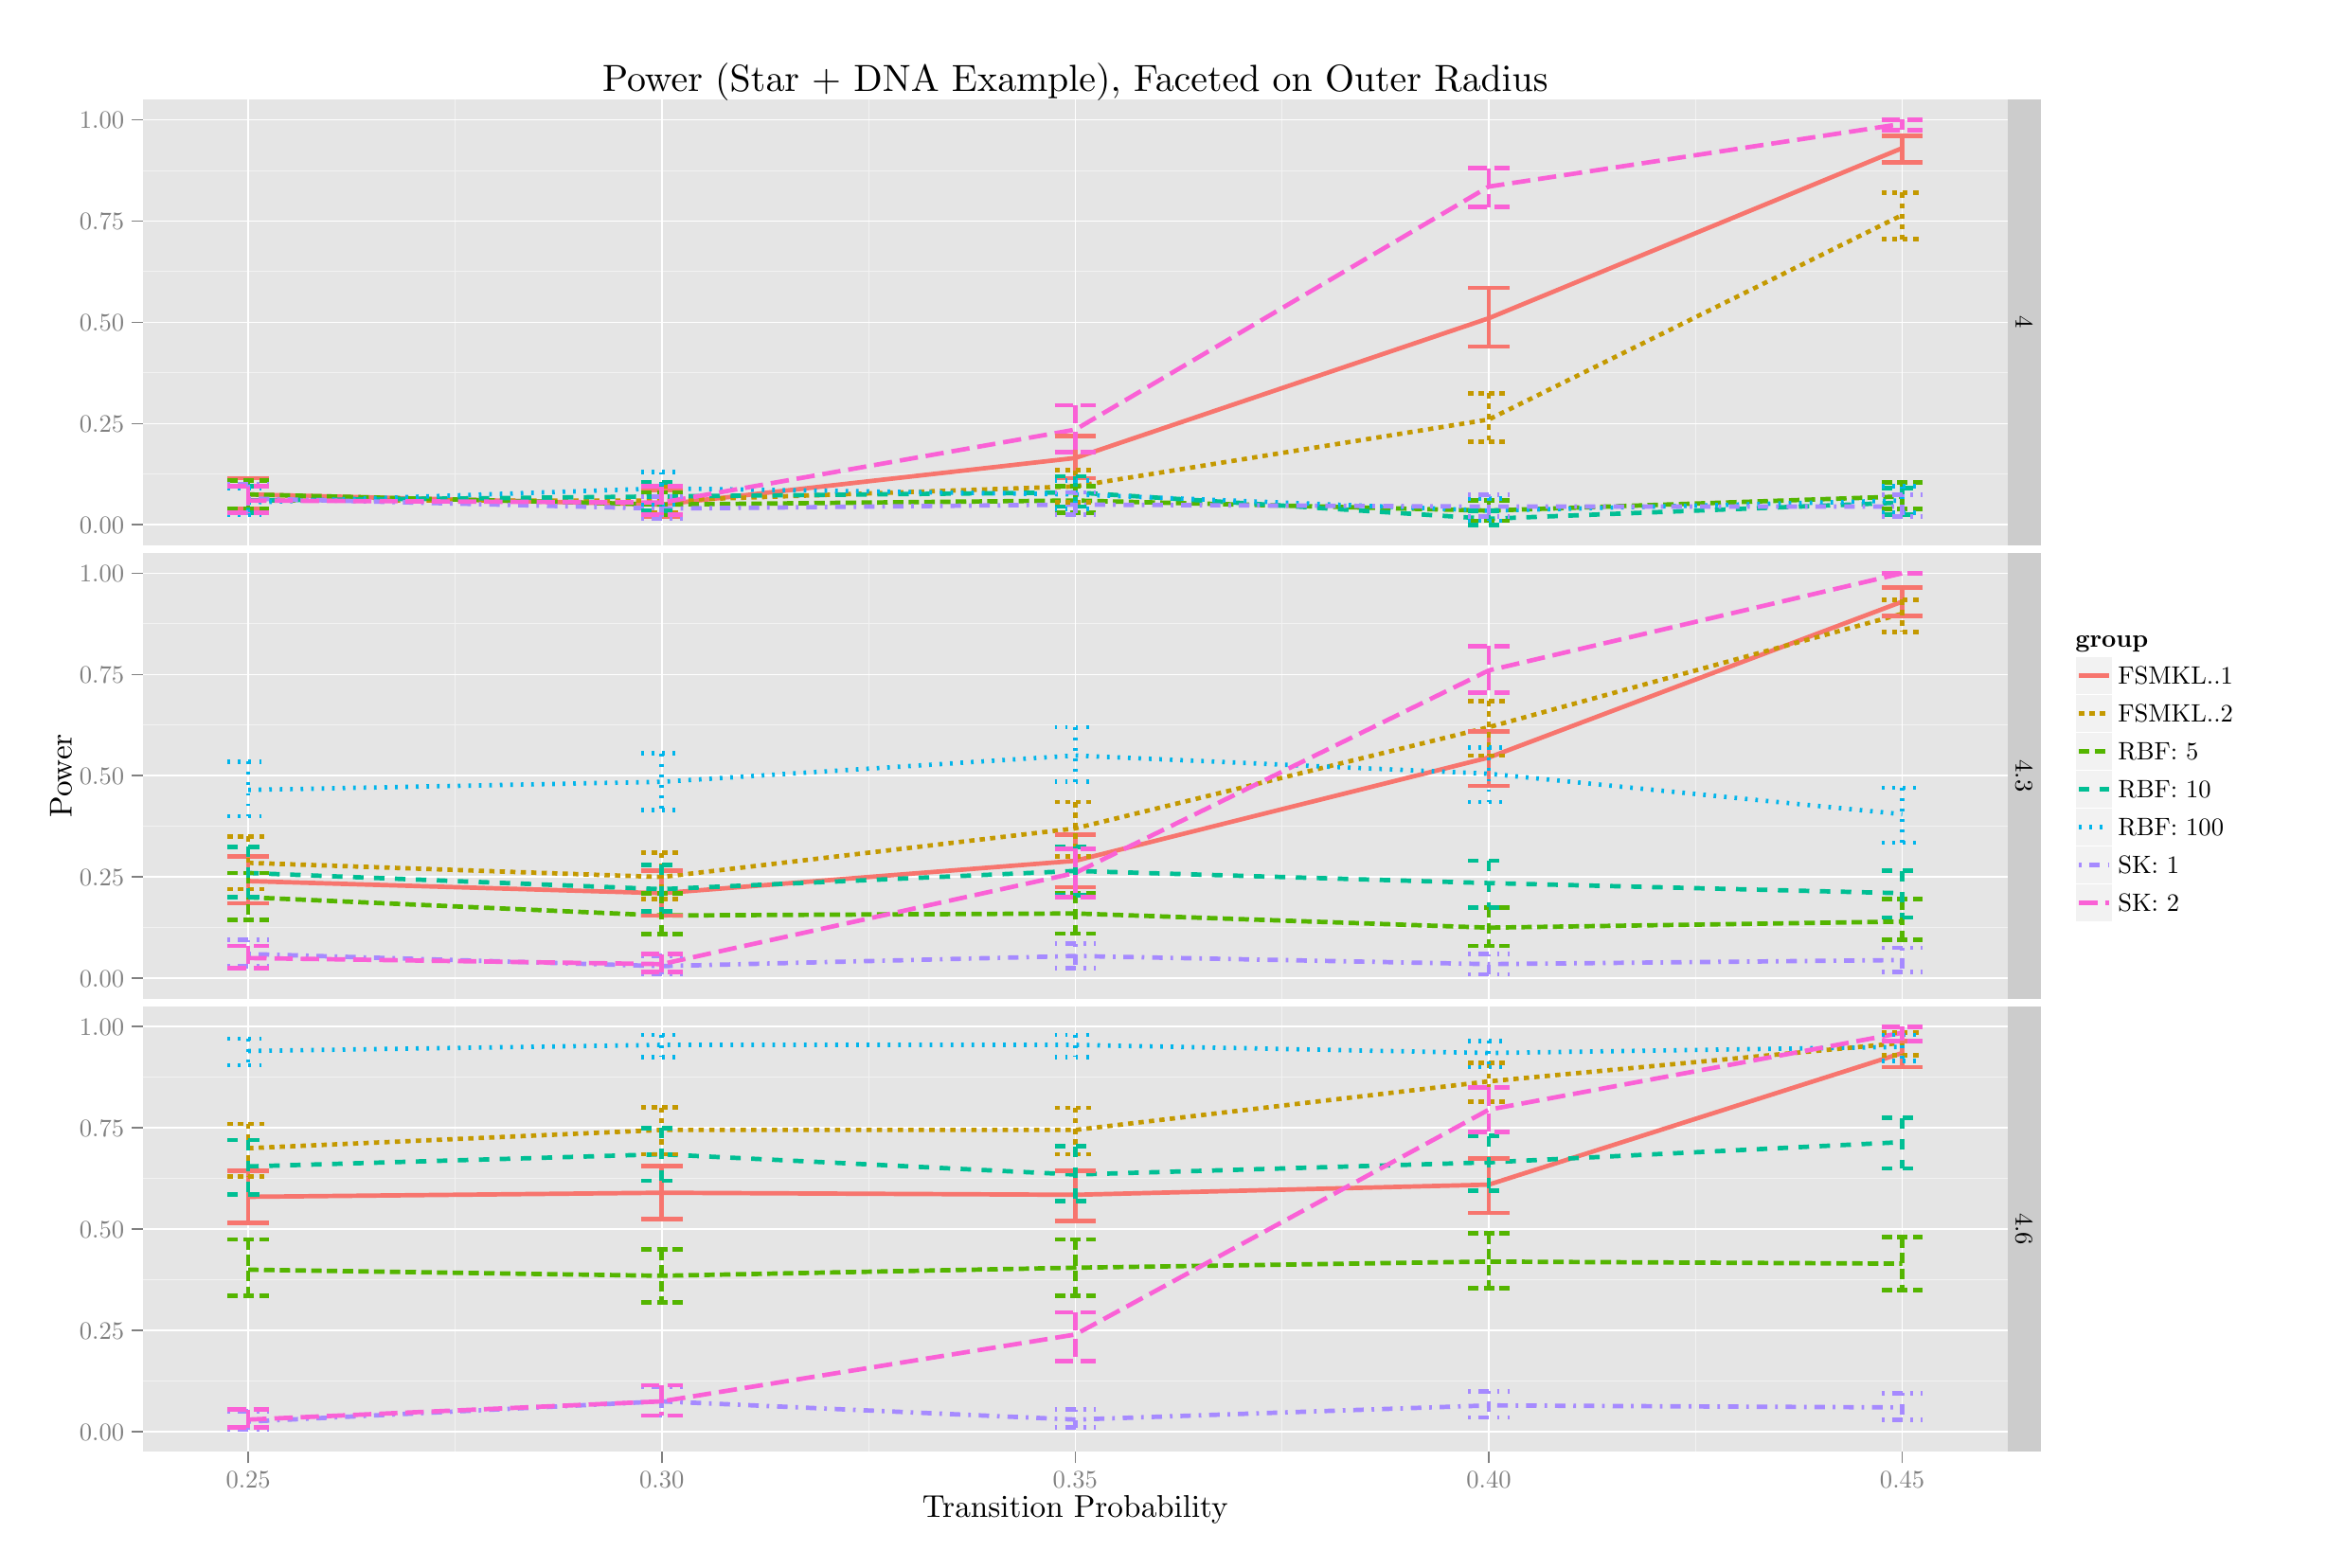
\begin{tikzpicture}[x=1pt,y=1pt]
\definecolor[named]{fillColor}{rgb}{1.00,1.00,1.00}
\path[use as bounding box,fill=fillColor,fill opacity=0.00] (0,0) rectangle (867.24,578.16);
\begin{scope}
\path[clip] (  0.00,  0.00) rectangle (867.24,578.16);
\definecolor[named]{drawColor}{rgb}{1.00,1.00,1.00}
\definecolor[named]{fillColor}{rgb}{1.00,1.00,1.00}

\path[draw=drawColor,line width= 0.6pt,line join=round,line cap=round,fill=fillColor] ( -0.00, -0.00) rectangle (867.24,578.16);
\end{scope}
\begin{scope}
\path[clip] ( 44.49,380.14) rectangle (756.04,550.17);
\definecolor[named]{fillColor}{rgb}{0.90,0.90,0.90}

\path[fill=fillColor] ( 44.49,380.14) rectangle (756.04,550.17);
\definecolor[named]{drawColor}{rgb}{0.95,0.95,0.95}

\path[draw=drawColor,line width= 0.3pt,line join=round] ( 44.49,407.19) --
	(756.04,407.19);

\path[draw=drawColor,line width= 0.3pt,line join=round] ( 44.49,445.83) --
	(756.04,445.83);

\path[draw=drawColor,line width= 0.3pt,line join=round] ( 44.49,484.48) --
	(756.04,484.48);

\path[draw=drawColor,line width= 0.3pt,line join=round] ( 44.49,523.12) --
	(756.04,523.12);

\path[draw=drawColor,line width= 0.3pt,line join=round] (163.60,380.14) --
	(163.60,550.17);

\path[draw=drawColor,line width= 0.3pt,line join=round] (321.38,380.14) --
	(321.38,550.17);

\path[draw=drawColor,line width= 0.3pt,line join=round] (479.15,380.14) --
	(479.15,550.17);

\path[draw=drawColor,line width= 0.3pt,line join=round] (636.92,380.14) --
	(636.92,550.17);
\definecolor[named]{drawColor}{rgb}{1.00,1.00,1.00}

\path[draw=drawColor,line width= 0.6pt,line join=round] ( 44.49,387.86) --
	(756.04,387.86);

\path[draw=drawColor,line width= 0.6pt,line join=round] ( 44.49,426.51) --
	(756.04,426.51);

\path[draw=drawColor,line width= 0.6pt,line join=round] ( 44.49,465.16) --
	(756.04,465.16);

\path[draw=drawColor,line width= 0.6pt,line join=round] ( 44.49,503.80) --
	(756.04,503.80);

\path[draw=drawColor,line width= 0.6pt,line join=round] ( 44.49,542.45) --
	(756.04,542.45);

\path[draw=drawColor,line width= 0.6pt,line join=round] ( 84.72,380.14) --
	( 84.72,550.17);

\path[draw=drawColor,line width= 0.6pt,line join=round] (242.49,380.14) --
	(242.49,550.17);

\path[draw=drawColor,line width= 0.6pt,line join=round] (400.26,380.14) --
	(400.26,550.17);

\path[draw=drawColor,line width= 0.6pt,line join=round] (558.03,380.14) --
	(558.03,550.17);

\path[draw=drawColor,line width= 0.6pt,line join=round] (715.81,380.14) --
	(715.81,550.17);
\definecolor[named]{drawColor}{rgb}{0.97,0.46,0.43}

\path[draw=drawColor,line width= 1.7pt,line join=round] ( 84.72,399.46) --
	(242.49,395.59) --
	(400.26,413.37) --
	(558.03,466.70) --
	(715.81,531.63);
\definecolor[named]{drawColor}{rgb}{0.77,0.60,0.00}

\path[draw=drawColor,line width= 1.7pt,dash pattern=on 2pt off 2pt ,line join=round] ( 84.72,397.14) --
	(242.49,397.14) --
	(400.26,402.55) --
	(558.03,428.06) --
	(715.81,506.12);
\definecolor[named]{drawColor}{rgb}{0.33,0.71,0.00}

\path[draw=drawColor,line width= 1.7pt,dash pattern=on 4pt off 2pt ,line join=round] ( 84.72,399.46) --
	(242.49,395.59) --
	(400.26,397.14) --
	(558.03,393.28) --
	(715.81,398.69);
\definecolor[named]{drawColor}{rgb}{0.00,0.75,0.58}

\path[draw=drawColor,line width= 1.7pt,dash pattern=on 4pt off 4pt ,line join=round] ( 84.72,397.14) --
	(242.49,398.69) --
	(400.26,400.23) --
	(558.03,390.18) --
	(715.81,396.37);
\definecolor[named]{drawColor}{rgb}{0.00,0.71,0.92}

\path[draw=drawColor,line width= 1.7pt,dash pattern=on 1pt off 3pt ,line join=round] ( 84.72,396.37) --
	(242.49,401.78) --
	(400.26,399.46) --
	(558.03,393.28) --
	(715.81,397.14);
\definecolor[named]{drawColor}{rgb}{0.65,0.54,1.00}

\path[draw=drawColor,line width= 1.7pt,dash pattern=on 1pt off 3pt on 4pt off 3pt ,line join=round] ( 84.72,397.91) --
	(242.49,394.05) --
	(400.26,395.59) --
	(558.03,394.82) --
	(715.81,394.82);
\definecolor[named]{drawColor}{rgb}{0.98,0.38,0.84}

\path[draw=drawColor,line width= 1.7pt,dash pattern=on 7pt off 3pt ,line join=round] ( 84.72,397.14) --
	(242.49,396.37) --
	(400.26,424.19) --
	(558.03,516.94) --
	(715.81,540.90);
\definecolor[named]{drawColor}{rgb}{0.97,0.46,0.43}

\path[draw=drawColor,line width= 1.7pt,line join=round] ( 76.83,405.64) --
	( 92.61,405.64);

\path[draw=drawColor,line width= 1.7pt,line join=round] ( 84.72,405.64) --
	( 84.72,394.05);

\path[draw=drawColor,line width= 1.7pt,line join=round] ( 76.83,394.05) --
	( 92.61,394.05);

\path[draw=drawColor,line width= 1.7pt,line join=round] (234.60,401.00) --
	(250.38,401.00);

\path[draw=drawColor,line width= 1.7pt,line join=round] (242.49,401.00) --
	(242.49,390.96);

\path[draw=drawColor,line width= 1.7pt,line join=round] (234.60,390.96) --
	(250.38,390.96);

\path[draw=drawColor,line width= 1.7pt,line join=round] (392.37,421.87) --
	(408.15,421.87);

\path[draw=drawColor,line width= 1.7pt,line join=round] (400.26,421.87) --
	(400.26,405.64);

\path[draw=drawColor,line width= 1.7pt,line join=round] (392.37,405.64) --
	(408.15,405.64);

\path[draw=drawColor,line width= 1.7pt,line join=round] (550.15,478.29) --
	(565.92,478.29);

\path[draw=drawColor,line width= 1.7pt,line join=round] (558.03,478.29) --
	(558.03,455.88);

\path[draw=drawColor,line width= 1.7pt,line join=round] (550.15,455.88) --
	(565.92,455.88);

\path[draw=drawColor,line width= 1.7pt,line join=round] (707.92,536.26) --
	(723.70,536.26);

\path[draw=drawColor,line width= 1.7pt,line join=round] (715.81,536.26) --
	(715.81,526.21);

\path[draw=drawColor,line width= 1.7pt,line join=round] (707.92,526.21) --
	(723.70,526.21);
\definecolor[named]{drawColor}{rgb}{0.77,0.60,0.00}

\path[draw=drawColor,line width= 1.7pt,dash pattern=on 2pt off 2pt ,line join=round] ( 76.83,402.55) --
	( 92.61,402.55);

\path[draw=drawColor,line width= 1.7pt,dash pattern=on 2pt off 2pt ,line join=round] ( 84.72,402.55) --
	( 84.72,392.50);

\path[draw=drawColor,line width= 1.7pt,dash pattern=on 2pt off 2pt ,line join=round] ( 76.83,392.50) --
	( 92.61,392.50);

\path[draw=drawColor,line width= 1.7pt,dash pattern=on 2pt off 2pt ,line join=round] (234.60,402.55) --
	(250.38,402.55);

\path[draw=drawColor,line width= 1.7pt,dash pattern=on 2pt off 2pt ,line join=round] (242.49,402.55) --
	(242.49,392.50);

\path[draw=drawColor,line width= 1.7pt,dash pattern=on 2pt off 2pt ,line join=round] (234.60,392.50) --
	(250.38,392.50);

\path[draw=drawColor,line width= 1.7pt,dash pattern=on 2pt off 2pt ,line join=round] (392.37,408.73) --
	(408.15,408.73);

\path[draw=drawColor,line width= 1.7pt,dash pattern=on 2pt off 2pt ,line join=round] (400.26,408.73) --
	(400.26,396.37);

\path[draw=drawColor,line width= 1.7pt,dash pattern=on 2pt off 2pt ,line join=round] (392.37,396.37) --
	(408.15,396.37);

\path[draw=drawColor,line width= 1.7pt,dash pattern=on 2pt off 2pt ,line join=round] (550.15,438.10) --
	(565.92,438.10);

\path[draw=drawColor,line width= 1.7pt,dash pattern=on 2pt off 2pt ,line join=round] (558.03,438.10) --
	(558.03,419.55);

\path[draw=drawColor,line width= 1.7pt,dash pattern=on 2pt off 2pt ,line join=round] (550.15,419.55) --
	(565.92,419.55);

\path[draw=drawColor,line width= 1.7pt,dash pattern=on 2pt off 2pt ,line join=round] (707.92,514.62) --
	(723.70,514.62);

\path[draw=drawColor,line width= 1.7pt,dash pattern=on 2pt off 2pt ,line join=round] (715.81,514.62) --
	(715.81,496.84);

\path[draw=drawColor,line width= 1.7pt,dash pattern=on 2pt off 2pt ,line join=round] (707.92,496.84) --
	(723.70,496.84);
\definecolor[named]{drawColor}{rgb}{0.33,0.71,0.00}

\path[draw=drawColor,line width= 1.7pt,dash pattern=on 4pt off 2pt ,line join=round] ( 76.83,404.87) --
	( 92.61,404.87);

\path[draw=drawColor,line width= 1.7pt,dash pattern=on 4pt off 2pt ,line join=round] ( 84.72,404.87) --
	( 84.72,394.05);

\path[draw=drawColor,line width= 1.7pt,dash pattern=on 4pt off 2pt ,line join=round] ( 76.83,394.05) --
	( 92.61,394.05);

\path[draw=drawColor,line width= 1.7pt,dash pattern=on 4pt off 2pt ,line join=round] (234.60,400.23) --
	(250.38,400.23);

\path[draw=drawColor,line width= 1.7pt,dash pattern=on 4pt off 2pt ,line join=round] (242.49,400.23) --
	(242.49,391.71);

\path[draw=drawColor,line width= 1.7pt,dash pattern=on 4pt off 2pt ,line join=round] (234.60,391.71) --
	(250.38,391.71);

\path[draw=drawColor,line width= 1.7pt,dash pattern=on 4pt off 2pt ,line join=round] (392.37,402.55) --
	(408.15,402.55);

\path[draw=drawColor,line width= 1.7pt,dash pattern=on 4pt off 2pt ,line join=round] (400.26,402.55) --
	(400.26,392.50);

\path[draw=drawColor,line width= 1.7pt,dash pattern=on 4pt off 2pt ,line join=round] (392.37,392.50) --
	(408.15,392.50);

\path[draw=drawColor,line width= 1.7pt,dash pattern=on 4pt off 2pt ,line join=round] (550.15,397.14) --
	(565.92,397.14);

\path[draw=drawColor,line width= 1.7pt,dash pattern=on 4pt off 2pt ,line join=round] (558.03,397.14) --
	(558.03,389.41);

\path[draw=drawColor,line width= 1.7pt,dash pattern=on 4pt off 2pt ,line join=round] (550.15,389.41) --
	(565.92,389.41);

\path[draw=drawColor,line width= 1.7pt,dash pattern=on 4pt off 2pt ,line join=round] (707.92,404.10) --
	(723.70,404.10);

\path[draw=drawColor,line width= 1.7pt,dash pattern=on 4pt off 2pt ,line join=round] (715.81,404.10) --
	(715.81,394.05);

\path[draw=drawColor,line width= 1.7pt,dash pattern=on 4pt off 2pt ,line join=round] (707.92,394.05) --
	(723.70,394.05);
\definecolor[named]{drawColor}{rgb}{0.00,0.75,0.58}

\path[draw=drawColor,line width= 1.7pt,dash pattern=on 4pt off 4pt ,line join=round] ( 76.83,402.55) --
	( 92.61,402.55);

\path[draw=drawColor,line width= 1.7pt,dash pattern=on 4pt off 4pt ,line join=round] ( 84.72,402.55) --
	( 84.72,392.50);

\path[draw=drawColor,line width= 1.7pt,dash pattern=on 4pt off 4pt ,line join=round] ( 76.83,392.50) --
	( 92.61,392.50);

\path[draw=drawColor,line width= 1.7pt,dash pattern=on 4pt off 4pt ,line join=round] (234.60,404.10) --
	(250.38,404.10);

\path[draw=drawColor,line width= 1.7pt,dash pattern=on 4pt off 4pt ,line join=round] (242.49,404.10) --
	(242.49,393.28);

\path[draw=drawColor,line width= 1.7pt,dash pattern=on 4pt off 4pt ,line join=round] (234.60,393.28) --
	(250.38,393.28);

\path[draw=drawColor,line width= 1.7pt,dash pattern=on 4pt off 4pt ,line join=round] (392.37,406.41) --
	(408.15,406.41);

\path[draw=drawColor,line width= 1.7pt,dash pattern=on 4pt off 4pt ,line join=round] (400.26,406.41) --
	(400.26,394.82);

\path[draw=drawColor,line width= 1.7pt,dash pattern=on 4pt off 4pt ,line join=round] (392.37,394.82) --
	(408.15,394.82);

\path[draw=drawColor,line width= 1.7pt,dash pattern=on 4pt off 4pt ,line join=round] (550.15,393.28) --
	(565.92,393.28);

\path[draw=drawColor,line width= 1.7pt,dash pattern=on 4pt off 4pt ,line join=round] (558.03,393.28) --
	(558.03,387.86);

\path[draw=drawColor,line width= 1.7pt,dash pattern=on 4pt off 4pt ,line join=round] (550.15,387.86) --
	(565.92,387.86);

\path[draw=drawColor,line width= 1.7pt,dash pattern=on 4pt off 4pt ,line join=round] (707.92,401.78) --
	(723.70,401.78);

\path[draw=drawColor,line width= 1.7pt,dash pattern=on 4pt off 4pt ,line join=round] (715.81,401.78) --
	(715.81,391.73);

\path[draw=drawColor,line width= 1.7pt,dash pattern=on 4pt off 4pt ,line join=round] (707.92,391.73) --
	(723.70,391.73);
\definecolor[named]{drawColor}{rgb}{0.00,0.71,0.92}

\path[draw=drawColor,line width= 1.7pt,dash pattern=on 1pt off 3pt ,line join=round] ( 76.83,401.78) --
	( 92.61,401.78);

\path[draw=drawColor,line width= 1.7pt,dash pattern=on 1pt off 3pt ,line join=round] ( 84.72,401.78) --
	( 84.72,391.73);

\path[draw=drawColor,line width= 1.7pt,dash pattern=on 1pt off 3pt ,line join=round] ( 76.83,391.73) --
	( 92.61,391.73);

\path[draw=drawColor,line width= 1.7pt,dash pattern=on 1pt off 3pt ,line join=round] (234.60,407.96) --
	(250.38,407.96);

\path[draw=drawColor,line width= 1.7pt,dash pattern=on 1pt off 3pt ,line join=round] (242.49,407.96) --
	(242.49,395.59);

\path[draw=drawColor,line width= 1.7pt,dash pattern=on 1pt off 3pt ,line join=round] (234.60,395.59) --
	(250.38,395.59);

\path[draw=drawColor,line width= 1.7pt,dash pattern=on 1pt off 3pt ,line join=round] (392.37,404.89) --
	(408.15,404.89);

\path[draw=drawColor,line width= 1.7pt,dash pattern=on 1pt off 3pt ,line join=round] (400.26,404.89) --
	(400.26,394.05);

\path[draw=drawColor,line width= 1.7pt,dash pattern=on 1pt off 3pt ,line join=round] (392.37,394.05) --
	(408.15,394.05);

\path[draw=drawColor,line width= 1.7pt,dash pattern=on 1pt off 3pt ,line join=round] (550.15,397.91) --
	(565.92,397.91);

\path[draw=drawColor,line width= 1.7pt,dash pattern=on 1pt off 3pt ,line join=round] (558.03,397.91) --
	(558.03,389.41);

\path[draw=drawColor,line width= 1.7pt,dash pattern=on 1pt off 3pt ,line join=round] (550.15,389.41) --
	(565.92,389.41);

\path[draw=drawColor,line width= 1.7pt,dash pattern=on 1pt off 3pt ,line join=round] (707.92,402.55) --
	(723.70,402.55);

\path[draw=drawColor,line width= 1.7pt,dash pattern=on 1pt off 3pt ,line join=round] (715.81,402.55) --
	(715.81,392.50);

\path[draw=drawColor,line width= 1.7pt,dash pattern=on 1pt off 3pt ,line join=round] (707.92,392.50) --
	(723.70,392.50);
\definecolor[named]{drawColor}{rgb}{0.65,0.54,1.00}

\path[draw=drawColor,line width= 1.7pt,dash pattern=on 1pt off 3pt on 4pt off 3pt ,line join=round] ( 76.83,403.32) --
	( 92.61,403.32);

\path[draw=drawColor,line width= 1.7pt,dash pattern=on 1pt off 3pt on 4pt off 3pt ,line join=round] ( 84.72,403.32) --
	( 84.72,392.50);

\path[draw=drawColor,line width= 1.7pt,dash pattern=on 1pt off 3pt on 4pt off 3pt ,line join=round] ( 76.83,392.50) --
	( 92.61,392.50);

\path[draw=drawColor,line width= 1.7pt,dash pattern=on 1pt off 3pt on 4pt off 3pt ,line join=round] (234.60,398.69) --
	(250.38,398.69);

\path[draw=drawColor,line width= 1.7pt,dash pattern=on 1pt off 3pt on 4pt off 3pt ,line join=round] (242.49,398.69) --
	(242.49,390.18);

\path[draw=drawColor,line width= 1.7pt,dash pattern=on 1pt off 3pt on 4pt off 3pt ,line join=round] (234.60,390.18) --
	(250.38,390.18);

\path[draw=drawColor,line width= 1.7pt,dash pattern=on 1pt off 3pt on 4pt off 3pt ,line join=round] (392.37,400.25) --
	(408.15,400.25);

\path[draw=drawColor,line width= 1.7pt,dash pattern=on 1pt off 3pt on 4pt off 3pt ,line join=round] (400.26,400.25) --
	(400.26,391.73);

\path[draw=drawColor,line width= 1.7pt,dash pattern=on 1pt off 3pt on 4pt off 3pt ,line join=round] (392.37,391.73) --
	(408.15,391.73);

\path[draw=drawColor,line width= 1.7pt,dash pattern=on 1pt off 3pt on 4pt off 3pt ,line join=round] (550.15,399.46) --
	(565.92,399.46);

\path[draw=drawColor,line width= 1.7pt,dash pattern=on 1pt off 3pt on 4pt off 3pt ,line join=round] (558.03,399.46) --
	(558.03,390.96);

\path[draw=drawColor,line width= 1.7pt,dash pattern=on 1pt off 3pt on 4pt off 3pt ,line join=round] (550.15,390.96) --
	(565.92,390.96);

\path[draw=drawColor,line width= 1.7pt,dash pattern=on 1pt off 3pt on 4pt off 3pt ,line join=round] (707.92,399.46) --
	(723.70,399.46);

\path[draw=drawColor,line width= 1.7pt,dash pattern=on 1pt off 3pt on 4pt off 3pt ,line join=round] (715.81,399.46) --
	(715.81,390.96);

\path[draw=drawColor,line width= 1.7pt,dash pattern=on 1pt off 3pt on 4pt off 3pt ,line join=round] (707.92,390.96) --
	(723.70,390.96);
\definecolor[named]{drawColor}{rgb}{0.98,0.38,0.84}

\path[draw=drawColor,line width= 1.7pt,dash pattern=on 7pt off 3pt ,line join=round] ( 76.83,402.55) --
	( 92.61,402.55);

\path[draw=drawColor,line width= 1.7pt,dash pattern=on 7pt off 3pt ,line join=round] ( 84.72,402.55) --
	( 84.72,392.50);

\path[draw=drawColor,line width= 1.7pt,dash pattern=on 7pt off 3pt ,line join=round] ( 76.83,392.50) --
	( 92.61,392.50);

\path[draw=drawColor,line width= 1.7pt,dash pattern=on 7pt off 3pt ,line join=round] (234.60,402.55) --
	(250.38,402.55);

\path[draw=drawColor,line width= 1.7pt,dash pattern=on 7pt off 3pt ,line join=round] (242.49,402.55) --
	(242.49,391.73);

\path[draw=drawColor,line width= 1.7pt,dash pattern=on 7pt off 3pt ,line join=round] (234.60,391.73) --
	(250.38,391.73);

\path[draw=drawColor,line width= 1.7pt,dash pattern=on 7pt off 3pt ,line join=round] (392.37,433.47) --
	(408.15,433.47);

\path[draw=drawColor,line width= 1.7pt,dash pattern=on 7pt off 3pt ,line join=round] (400.26,433.47) --
	(400.26,415.69);

\path[draw=drawColor,line width= 1.7pt,dash pattern=on 7pt off 3pt ,line join=round] (392.37,415.69) --
	(408.15,415.69);

\path[draw=drawColor,line width= 1.7pt,dash pattern=on 7pt off 3pt ,line join=round] (550.15,523.90) --
	(565.92,523.90);

\path[draw=drawColor,line width= 1.7pt,dash pattern=on 7pt off 3pt ,line join=round] (558.03,523.90) --
	(558.03,509.19);

\path[draw=drawColor,line width= 1.7pt,dash pattern=on 7pt off 3pt ,line join=round] (550.15,509.19) --
	(565.92,509.19);

\path[draw=drawColor,line width= 1.7pt,dash pattern=on 7pt off 3pt ,line join=round] (707.92,542.45) --
	(723.70,542.45);

\path[draw=drawColor,line width= 1.7pt,dash pattern=on 7pt off 3pt ,line join=round] (715.81,542.45) --
	(715.81,538.58);

\path[draw=drawColor,line width= 1.7pt,dash pattern=on 7pt off 3pt ,line join=round] (707.92,538.58) --
	(723.70,538.58);
\end{scope}
\begin{scope}
\path[clip] ( 44.49,207.09) rectangle (756.04,377.12);
\definecolor[named]{fillColor}{rgb}{0.90,0.90,0.90}

\path[fill=fillColor] ( 44.49,207.09) rectangle (756.04,377.12);
\definecolor[named]{drawColor}{rgb}{0.95,0.95,0.95}

\path[draw=drawColor,line width= 0.3pt,line join=round] ( 44.49,234.14) --
	(756.04,234.14);

\path[draw=drawColor,line width= 0.3pt,line join=round] ( 44.49,272.78) --
	(756.04,272.78);

\path[draw=drawColor,line width= 0.3pt,line join=round] ( 44.49,311.43) --
	(756.04,311.43);

\path[draw=drawColor,line width= 0.3pt,line join=round] ( 44.49,350.07) --
	(756.04,350.07);

\path[draw=drawColor,line width= 0.3pt,line join=round] (163.60,207.09) --
	(163.60,377.12);

\path[draw=drawColor,line width= 0.3pt,line join=round] (321.38,207.09) --
	(321.38,377.12);

\path[draw=drawColor,line width= 0.3pt,line join=round] (479.15,207.09) --
	(479.15,377.12);

\path[draw=drawColor,line width= 0.3pt,line join=round] (636.92,207.09) --
	(636.92,377.12);
\definecolor[named]{drawColor}{rgb}{1.00,1.00,1.00}

\path[draw=drawColor,line width= 0.6pt,line join=round] ( 44.49,214.81) --
	(756.04,214.81);

\path[draw=drawColor,line width= 0.6pt,line join=round] ( 44.49,253.46) --
	(756.04,253.46);

\path[draw=drawColor,line width= 0.6pt,line join=round] ( 44.49,292.10) --
	(756.04,292.10);

\path[draw=drawColor,line width= 0.6pt,line join=round] ( 44.49,330.75) --
	(756.04,330.75);

\path[draw=drawColor,line width= 0.6pt,line join=round] ( 44.49,369.40) --
	(756.04,369.40);

\path[draw=drawColor,line width= 0.6pt,line join=round] ( 84.72,207.09) --
	( 84.72,377.12);

\path[draw=drawColor,line width= 0.6pt,line join=round] (242.49,207.09) --
	(242.49,377.12);

\path[draw=drawColor,line width= 0.6pt,line join=round] (400.26,207.09) --
	(400.26,377.12);

\path[draw=drawColor,line width= 0.6pt,line join=round] (558.03,207.09) --
	(558.03,377.12);

\path[draw=drawColor,line width= 0.6pt,line join=round] (715.81,207.09) --
	(715.81,377.12);
\definecolor[named]{drawColor}{rgb}{0.97,0.46,0.43}

\path[draw=drawColor,line width= 1.7pt,line join=round] ( 84.72,251.91) --
	(242.49,247.28) --
	(400.26,259.64) --
	(558.03,299.06) --
	(715.81,358.57);
\definecolor[named]{drawColor}{rgb}{0.77,0.60,0.00}

\path[draw=drawColor,line width= 1.7pt,dash pattern=on 2pt off 2pt ,line join=round] ( 84.72,258.87) --
	(242.49,253.46) --
	(400.26,272.01) --
	(558.03,310.65) --
	(715.81,353.94);
\definecolor[named]{drawColor}{rgb}{0.33,0.71,0.00}

\path[draw=drawColor,line width= 1.7pt,dash pattern=on 4pt off 2pt ,line join=round] ( 84.72,245.73) --
	(242.49,238.77) --
	(400.26,239.55) --
	(558.03,234.14) --
	(715.81,236.46);
\definecolor[named]{drawColor}{rgb}{0.00,0.75,0.58}

\path[draw=drawColor,line width= 1.7pt,dash pattern=on 4pt off 4pt ,line join=round] ( 84.72,255.01) --
	(242.49,248.82) --
	(400.26,255.78) --
	(558.03,251.14) --
	(715.81,247.28);
\definecolor[named]{drawColor}{rgb}{0.00,0.71,0.92}

\path[draw=drawColor,line width= 1.7pt,dash pattern=on 1pt off 3pt ,line join=round] ( 84.72,286.69) --
	(242.49,289.79) --
	(400.26,299.83) --
	(558.03,292.88) --
	(715.81,277.42);
\definecolor[named]{drawColor}{rgb}{0.65,0.54,1.00}

\path[draw=drawColor,line width= 1.7pt,dash pattern=on 1pt off 3pt on 4pt off 3pt ,line join=round] ( 84.72,224.09) --
	(242.49,219.45) --
	(400.26,223.32) --
	(558.03,220.22) --
	(715.81,221.77);
\definecolor[named]{drawColor}{rgb}{0.98,0.38,0.84}

\path[draw=drawColor,line width= 1.7pt,dash pattern=on 7pt off 3pt ,line join=round] ( 84.72,222.54) --
	(242.49,220.22) --
	(400.26,255.01) --
	(558.03,332.30) --
	(715.81,369.40);
\definecolor[named]{drawColor}{rgb}{0.97,0.46,0.43}

\path[draw=drawColor,line width= 1.7pt,line join=round] ( 76.83,261.19) --
	( 92.61,261.19);

\path[draw=drawColor,line width= 1.7pt,line join=round] ( 84.72,261.19) --
	( 84.72,243.41);

\path[draw=drawColor,line width= 1.7pt,line join=round] ( 76.83,243.41) --
	( 92.61,243.41);

\path[draw=drawColor,line width= 1.7pt,line join=round] (234.60,255.78) --
	(250.38,255.78);

\path[draw=drawColor,line width= 1.7pt,line join=round] (242.49,255.78) --
	(242.49,238.77);

\path[draw=drawColor,line width= 1.7pt,line join=round] (234.60,238.77) --
	(250.38,238.77);

\path[draw=drawColor,line width= 1.7pt,line join=round] (392.37,269.69) --
	(408.15,269.69);

\path[draw=drawColor,line width= 1.7pt,line join=round] (400.26,269.69) --
	(400.26,249.59);

\path[draw=drawColor,line width= 1.7pt,line join=round] (392.37,249.59) --
	(408.15,249.59);

\path[draw=drawColor,line width= 1.7pt,line join=round] (550.15,309.11) --
	(565.92,309.11);

\path[draw=drawColor,line width= 1.7pt,line join=round] (558.03,309.11) --
	(558.03,288.24);

\path[draw=drawColor,line width= 1.7pt,line join=round] (550.15,288.24) --
	(565.92,288.24);

\path[draw=drawColor,line width= 1.7pt,line join=round] (707.92,363.98) --
	(723.70,363.98);

\path[draw=drawColor,line width= 1.7pt,line join=round] (715.81,363.98) --
	(715.81,353.16);

\path[draw=drawColor,line width= 1.7pt,line join=round] (707.92,353.16) --
	(723.70,353.16);
\definecolor[named]{drawColor}{rgb}{0.77,0.60,0.00}

\path[draw=drawColor,line width= 1.7pt,dash pattern=on 2pt off 2pt ,line join=round] ( 76.83,268.92) --
	( 92.61,268.92);

\path[draw=drawColor,line width= 1.7pt,dash pattern=on 2pt off 2pt ,line join=round] ( 84.72,268.92) --
	( 84.72,248.82);

\path[draw=drawColor,line width= 1.7pt,dash pattern=on 2pt off 2pt ,line join=round] ( 76.83,248.82) --
	( 92.61,248.82);

\path[draw=drawColor,line width= 1.7pt,dash pattern=on 2pt off 2pt ,line join=round] (234.60,262.73) --
	(250.38,262.73);

\path[draw=drawColor,line width= 1.7pt,dash pattern=on 2pt off 2pt ,line join=round] (242.49,262.73) --
	(242.49,244.96);

\path[draw=drawColor,line width= 1.7pt,dash pattern=on 2pt off 2pt ,line join=round] (234.60,244.96) --
	(250.38,244.96);

\path[draw=drawColor,line width= 1.7pt,dash pattern=on 2pt off 2pt ,line join=round] (392.37,282.06) --
	(408.15,282.06);

\path[draw=drawColor,line width= 1.7pt,dash pattern=on 2pt off 2pt ,line join=round] (400.26,282.06) --
	(400.26,261.19);

\path[draw=drawColor,line width= 1.7pt,dash pattern=on 2pt off 2pt ,line join=round] (392.37,261.19) --
	(408.15,261.19);

\path[draw=drawColor,line width= 1.7pt,dash pattern=on 2pt off 2pt ,line join=round] (550.15,320.70) --
	(565.92,320.70);

\path[draw=drawColor,line width= 1.7pt,dash pattern=on 2pt off 2pt ,line join=round] (558.03,320.70) --
	(558.03,299.83);

\path[draw=drawColor,line width= 1.7pt,dash pattern=on 2pt off 2pt ,line join=round] (550.15,299.83) --
	(565.92,299.83);

\path[draw=drawColor,line width= 1.7pt,dash pattern=on 2pt off 2pt ,line join=round] (707.92,359.35) --
	(723.70,359.35);

\path[draw=drawColor,line width= 1.7pt,dash pattern=on 2pt off 2pt ,line join=round] (715.81,359.35) --
	(715.81,346.98);

\path[draw=drawColor,line width= 1.7pt,dash pattern=on 2pt off 2pt ,line join=round] (707.92,346.98) --
	(723.70,346.98);
\definecolor[named]{drawColor}{rgb}{0.33,0.71,0.00}

\path[draw=drawColor,line width= 1.7pt,dash pattern=on 4pt off 2pt ,line join=round] ( 76.83,255.01) --
	( 92.61,255.01);

\path[draw=drawColor,line width= 1.7pt,dash pattern=on 4pt off 2pt ,line join=round] ( 84.72,255.01) --
	( 84.72,237.23);

\path[draw=drawColor,line width= 1.7pt,dash pattern=on 4pt off 2pt ,line join=round] ( 76.83,237.23) --
	( 92.61,237.23);

\path[draw=drawColor,line width= 1.7pt,dash pattern=on 4pt off 2pt ,line join=round] (234.60,247.28) --
	(250.38,247.28);

\path[draw=drawColor,line width= 1.7pt,dash pattern=on 4pt off 2pt ,line join=round] (242.49,247.28) --
	(242.49,231.80);

\path[draw=drawColor,line width= 1.7pt,dash pattern=on 4pt off 2pt ,line join=round] (234.60,231.80) --
	(250.38,231.80);

\path[draw=drawColor,line width= 1.7pt,dash pattern=on 4pt off 2pt ,line join=round] (392.37,247.28) --
	(408.15,247.28);

\path[draw=drawColor,line width= 1.7pt,dash pattern=on 4pt off 2pt ,line join=round] (400.26,247.28) --
	(400.26,231.82);

\path[draw=drawColor,line width= 1.7pt,dash pattern=on 4pt off 2pt ,line join=round] (392.37,231.82) --
	(408.15,231.82);

\path[draw=drawColor,line width= 1.7pt,dash pattern=on 4pt off 2pt ,line join=round] (550.15,241.87) --
	(565.92,241.87);

\path[draw=drawColor,line width= 1.7pt,dash pattern=on 4pt off 2pt ,line join=round] (558.03,241.87) --
	(558.03,227.18);

\path[draw=drawColor,line width= 1.7pt,dash pattern=on 4pt off 2pt ,line join=round] (550.15,227.18) --
	(565.92,227.18);

\path[draw=drawColor,line width= 1.7pt,dash pattern=on 4pt off 2pt ,line join=round] (707.92,244.96) --
	(723.70,244.96);

\path[draw=drawColor,line width= 1.7pt,dash pattern=on 4pt off 2pt ,line join=round] (715.81,244.96) --
	(715.81,229.50);

\path[draw=drawColor,line width= 1.7pt,dash pattern=on 4pt off 2pt ,line join=round] (707.92,229.50) --
	(723.70,229.50);
\definecolor[named]{drawColor}{rgb}{0.00,0.75,0.58}

\path[draw=drawColor,line width= 1.7pt,dash pattern=on 4pt off 4pt ,line join=round] ( 76.83,265.05) --
	( 92.61,265.05);

\path[draw=drawColor,line width= 1.7pt,dash pattern=on 4pt off 4pt ,line join=round] ( 84.72,265.05) --
	( 84.72,245.73);

\path[draw=drawColor,line width= 1.7pt,dash pattern=on 4pt off 4pt ,line join=round] ( 76.83,245.73) --
	( 92.61,245.73);

\path[draw=drawColor,line width= 1.7pt,dash pattern=on 4pt off 4pt ,line join=round] (234.60,258.10) --
	(250.38,258.10);

\path[draw=drawColor,line width= 1.7pt,dash pattern=on 4pt off 4pt ,line join=round] (242.49,258.10) --
	(242.49,240.32);

\path[draw=drawColor,line width= 1.7pt,dash pattern=on 4pt off 4pt ,line join=round] (234.60,240.32) --
	(250.38,240.32);

\path[draw=drawColor,line width= 1.7pt,dash pattern=on 4pt off 4pt ,line join=round] (392.37,265.05) --
	(408.15,265.05);

\path[draw=drawColor,line width= 1.7pt,dash pattern=on 4pt off 4pt ,line join=round] (400.26,265.05) --
	(400.26,246.48);

\path[draw=drawColor,line width= 1.7pt,dash pattern=on 4pt off 4pt ,line join=round] (392.37,246.48) --
	(408.15,246.48);

\path[draw=drawColor,line width= 1.7pt,dash pattern=on 4pt off 4pt ,line join=round] (550.15,259.64) --
	(565.92,259.64);

\path[draw=drawColor,line width= 1.7pt,dash pattern=on 4pt off 4pt ,line join=round] (558.03,259.64) --
	(558.03,241.87);

\path[draw=drawColor,line width= 1.7pt,dash pattern=on 4pt off 4pt ,line join=round] (550.15,241.87) --
	(565.92,241.87);

\path[draw=drawColor,line width= 1.7pt,dash pattern=on 4pt off 4pt ,line join=round] (707.92,255.78) --
	(723.70,255.78);

\path[draw=drawColor,line width= 1.7pt,dash pattern=on 4pt off 4pt ,line join=round] (715.81,255.78) --
	(715.81,238.00);

\path[draw=drawColor,line width= 1.7pt,dash pattern=on 4pt off 4pt ,line join=round] (707.92,238.00) --
	(723.70,238.00);
\definecolor[named]{drawColor}{rgb}{0.00,0.71,0.92}

\path[draw=drawColor,line width= 1.7pt,dash pattern=on 1pt off 3pt ,line join=round] ( 76.83,297.52) --
	( 92.61,297.52);

\path[draw=drawColor,line width= 1.7pt,dash pattern=on 1pt off 3pt ,line join=round] ( 84.72,297.52) --
	( 84.72,276.65);

\path[draw=drawColor,line width= 1.7pt,dash pattern=on 1pt off 3pt ,line join=round] ( 76.83,276.65) --
	( 92.61,276.65);

\path[draw=drawColor,line width= 1.7pt,dash pattern=on 1pt off 3pt ,line join=round] (234.60,300.61) --
	(250.38,300.61);

\path[draw=drawColor,line width= 1.7pt,dash pattern=on 1pt off 3pt ,line join=round] (242.49,300.61) --
	(242.49,278.95);

\path[draw=drawColor,line width= 1.7pt,dash pattern=on 1pt off 3pt ,line join=round] (234.60,278.95) --
	(250.38,278.95);

\path[draw=drawColor,line width= 1.7pt,dash pattern=on 1pt off 3pt ,line join=round] (392.37,310.65) --
	(408.15,310.65);

\path[draw=drawColor,line width= 1.7pt,dash pattern=on 1pt off 3pt ,line join=round] (400.26,310.65) --
	(400.26,289.79);

\path[draw=drawColor,line width= 1.7pt,dash pattern=on 1pt off 3pt ,line join=round] (392.37,289.79) --
	(408.15,289.79);

\path[draw=drawColor,line width= 1.7pt,dash pattern=on 1pt off 3pt ,line join=round] (550.15,302.93) --
	(565.92,302.93);

\path[draw=drawColor,line width= 1.7pt,dash pattern=on 1pt off 3pt ,line join=round] (558.03,302.93) --
	(558.03,282.06);

\path[draw=drawColor,line width= 1.7pt,dash pattern=on 1pt off 3pt ,line join=round] (550.15,282.06) --
	(565.92,282.06);

\path[draw=drawColor,line width= 1.7pt,dash pattern=on 1pt off 3pt ,line join=round] (707.92,287.47) --
	(723.70,287.47);

\path[draw=drawColor,line width= 1.7pt,dash pattern=on 1pt off 3pt ,line join=round] (715.81,287.47) --
	(715.81,266.60);

\path[draw=drawColor,line width= 1.7pt,dash pattern=on 1pt off 3pt ,line join=round] (707.92,266.60) --
	(723.70,266.60);
\definecolor[named]{drawColor}{rgb}{0.65,0.54,1.00}

\path[draw=drawColor,line width= 1.7pt,dash pattern=on 1pt off 3pt on 4pt off 3pt ,line join=round] ( 76.83,229.50) --
	( 92.61,229.50);

\path[draw=drawColor,line width= 1.7pt,dash pattern=on 1pt off 3pt on 4pt off 3pt ,line join=round] ( 84.72,229.50) --
	( 84.72,219.45);

\path[draw=drawColor,line width= 1.7pt,dash pattern=on 1pt off 3pt on 4pt off 3pt ,line join=round] ( 76.83,219.45) --
	( 92.61,219.45);

\path[draw=drawColor,line width= 1.7pt,dash pattern=on 1pt off 3pt on 4pt off 3pt ,line join=round] (234.60,223.32) --
	(250.38,223.32);

\path[draw=drawColor,line width= 1.7pt,dash pattern=on 1pt off 3pt on 4pt off 3pt ,line join=round] (242.49,223.32) --
	(242.49,216.36);

\path[draw=drawColor,line width= 1.7pt,dash pattern=on 1pt off 3pt on 4pt off 3pt ,line join=round] (234.60,216.36) --
	(250.38,216.36);

\path[draw=drawColor,line width= 1.7pt,dash pattern=on 1pt off 3pt on 4pt off 3pt ,line join=round] (392.37,227.95) --
	(408.15,227.95);

\path[draw=drawColor,line width= 1.7pt,dash pattern=on 1pt off 3pt on 4pt off 3pt ,line join=round] (400.26,227.95) --
	(400.26,218.68);

\path[draw=drawColor,line width= 1.7pt,dash pattern=on 1pt off 3pt on 4pt off 3pt ,line join=round] (392.37,218.68) --
	(408.15,218.68);

\path[draw=drawColor,line width= 1.7pt,dash pattern=on 1pt off 3pt on 4pt off 3pt ,line join=round] (550.15,224.09) --
	(565.92,224.09);

\path[draw=drawColor,line width= 1.7pt,dash pattern=on 1pt off 3pt on 4pt off 3pt ,line join=round] (558.03,224.09) --
	(558.03,216.36);

\path[draw=drawColor,line width= 1.7pt,dash pattern=on 1pt off 3pt on 4pt off 3pt ,line join=round] (550.15,216.36) --
	(565.92,216.36);

\path[draw=drawColor,line width= 1.7pt,dash pattern=on 1pt off 3pt on 4pt off 3pt ,line join=round] (707.92,226.41) --
	(723.70,226.41);

\path[draw=drawColor,line width= 1.7pt,dash pattern=on 1pt off 3pt on 4pt off 3pt ,line join=round] (715.81,226.41) --
	(715.81,217.13);

\path[draw=drawColor,line width= 1.7pt,dash pattern=on 1pt off 3pt on 4pt off 3pt ,line join=round] (707.92,217.13) --
	(723.70,217.13);
\definecolor[named]{drawColor}{rgb}{0.98,0.38,0.84}

\path[draw=drawColor,line width= 1.7pt,dash pattern=on 7pt off 3pt ,line join=round] ( 76.83,227.18) --
	( 92.61,227.18);

\path[draw=drawColor,line width= 1.7pt,dash pattern=on 7pt off 3pt ,line join=round] ( 84.72,227.18) --
	( 84.72,218.68);

\path[draw=drawColor,line width= 1.7pt,dash pattern=on 7pt off 3pt ,line join=round] ( 76.83,218.68) --
	( 92.61,218.68);

\path[draw=drawColor,line width= 1.7pt,dash pattern=on 7pt off 3pt ,line join=round] (234.60,224.09) --
	(250.38,224.09);

\path[draw=drawColor,line width= 1.7pt,dash pattern=on 7pt off 3pt ,line join=round] (242.49,224.09) --
	(242.49,217.13);

\path[draw=drawColor,line width= 1.7pt,dash pattern=on 7pt off 3pt ,line join=round] (234.60,217.13) --
	(250.38,217.13);

\path[draw=drawColor,line width= 1.7pt,dash pattern=on 7pt off 3pt ,line join=round] (392.37,264.28) --
	(408.15,264.28);

\path[draw=drawColor,line width= 1.7pt,dash pattern=on 7pt off 3pt ,line join=round] (400.26,264.28) --
	(400.26,245.73);

\path[draw=drawColor,line width= 1.7pt,dash pattern=on 7pt off 3pt ,line join=round] (392.37,245.73) --
	(408.15,245.73);

\path[draw=drawColor,line width= 1.7pt,dash pattern=on 7pt off 3pt ,line join=round] (550.15,341.57) --
	(565.92,341.57);

\path[draw=drawColor,line width= 1.7pt,dash pattern=on 7pt off 3pt ,line join=round] (558.03,341.57) --
	(558.03,323.79);

\path[draw=drawColor,line width= 1.7pt,dash pattern=on 7pt off 3pt ,line join=round] (550.15,323.79) --
	(565.92,323.79);

\path[draw=drawColor,line width= 1.7pt,dash pattern=on 7pt off 3pt ,line join=round] (707.92,369.40) --
	(723.70,369.40);

\path[draw=drawColor,line width= 1.7pt,dash pattern=on 7pt off 3pt ,line join=round] (715.81,369.40) --
	(715.81,369.40);

\path[draw=drawColor,line width= 1.7pt,dash pattern=on 7pt off 3pt ,line join=round] (707.92,369.40) --
	(723.70,369.40);
\end{scope}
\begin{scope}
\path[clip] ( 44.49, 34.03) rectangle (756.04,204.07);
\definecolor[named]{fillColor}{rgb}{0.90,0.90,0.90}

\path[fill=fillColor] ( 44.49, 34.03) rectangle (756.04,204.07);
\definecolor[named]{drawColor}{rgb}{0.95,0.95,0.95}

\path[draw=drawColor,line width= 0.3pt,line join=round] ( 44.49, 61.09) --
	(756.04, 61.09);

\path[draw=drawColor,line width= 0.3pt,line join=round] ( 44.49, 99.73) --
	(756.04, 99.73);

\path[draw=drawColor,line width= 0.3pt,line join=round] ( 44.49,138.38) --
	(756.04,138.38);

\path[draw=drawColor,line width= 0.3pt,line join=round] ( 44.49,177.02) --
	(756.04,177.02);

\path[draw=drawColor,line width= 0.3pt,line join=round] (163.60, 34.03) --
	(163.60,204.07);

\path[draw=drawColor,line width= 0.3pt,line join=round] (321.38, 34.03) --
	(321.38,204.07);

\path[draw=drawColor,line width= 0.3pt,line join=round] (479.15, 34.03) --
	(479.15,204.07);

\path[draw=drawColor,line width= 0.3pt,line join=round] (636.92, 34.03) --
	(636.92,204.07);
\definecolor[named]{drawColor}{rgb}{1.00,1.00,1.00}

\path[draw=drawColor,line width= 0.6pt,line join=round] ( 44.49, 41.76) --
	(756.04, 41.76);

\path[draw=drawColor,line width= 0.6pt,line join=round] ( 44.49, 80.41) --
	(756.04, 80.41);

\path[draw=drawColor,line width= 0.6pt,line join=round] ( 44.49,119.05) --
	(756.04,119.05);

\path[draw=drawColor,line width= 0.6pt,line join=round] ( 44.49,157.70) --
	(756.04,157.70);

\path[draw=drawColor,line width= 0.6pt,line join=round] ( 44.49,196.34) --
	(756.04,196.34);

\path[draw=drawColor,line width= 0.6pt,line join=round] ( 84.72, 34.03) --
	( 84.72,204.07);

\path[draw=drawColor,line width= 0.6pt,line join=round] (242.49, 34.03) --
	(242.49,204.07);

\path[draw=drawColor,line width= 0.6pt,line join=round] (400.26, 34.03) --
	(400.26,204.07);

\path[draw=drawColor,line width= 0.6pt,line join=round] (558.03, 34.03) --
	(558.03,204.07);

\path[draw=drawColor,line width= 0.6pt,line join=round] (715.81, 34.03) --
	(715.81,204.07);
\definecolor[named]{drawColor}{rgb}{0.97,0.46,0.43}

\path[draw=drawColor,line width= 1.7pt,line join=round] ( 84.72,131.42) --
	(242.49,132.97) --
	(400.26,132.19) --
	(558.03,136.06) --
	(715.81,186.30);
\definecolor[named]{drawColor}{rgb}{0.77,0.60,0.00}

\path[draw=drawColor,line width= 1.7pt,dash pattern=on 2pt off 2pt ,line join=round] ( 84.72,149.97) --
	(242.49,156.93) --
	(400.26,156.93) --
	(558.03,175.48) --
	(715.81,190.16);
\definecolor[named]{drawColor}{rgb}{0.33,0.71,0.00}

\path[draw=drawColor,line width= 1.7pt,dash pattern=on 4pt off 2pt ,line join=round] ( 84.72,103.60) --
	(242.49,101.28) --
	(400.26,104.37) --
	(558.03,106.69) --
	(715.81,105.91);
\definecolor[named]{drawColor}{rgb}{0.00,0.75,0.58}

\path[draw=drawColor,line width= 1.7pt,dash pattern=on 4pt off 4pt ,line join=round] ( 84.72,143.01) --
	(242.49,147.65) --
	(400.26,139.92) --
	(558.03,144.56) --
	(715.81,152.29);
\definecolor[named]{drawColor}{rgb}{0.00,0.71,0.92}

\path[draw=drawColor,line width= 1.7pt,dash pattern=on 1pt off 3pt ,line join=round] ( 84.72,187.07) --
	(242.49,189.39) --
	(400.26,189.39) --
	(558.03,186.30) --
	(715.81,188.62);
\definecolor[named]{drawColor}{rgb}{0.65,0.54,1.00}

\path[draw=drawColor,line width= 1.7pt,dash pattern=on 1pt off 3pt on 4pt off 3pt ,line join=round] ( 84.72, 45.63) --
	(242.49, 53.36) --
	(400.26, 46.40) --
	(558.03, 51.81) --
	(715.81, 51.04);
\definecolor[named]{drawColor}{rgb}{0.98,0.38,0.84}

\path[draw=drawColor,line width= 1.7pt,dash pattern=on 7pt off 3pt ,line join=round] ( 84.72, 46.40) --
	(242.49, 53.36) --
	(400.26, 78.86) --
	(558.03,164.66) --
	(715.81,194.03);
\definecolor[named]{drawColor}{rgb}{0.97,0.46,0.43}

\path[draw=drawColor,line width= 1.7pt,line join=round] ( 76.83,141.47) --
	( 92.61,141.47);

\path[draw=drawColor,line width= 1.7pt,line join=round] ( 84.72,141.47) --
	( 84.72,121.37);

\path[draw=drawColor,line width= 1.7pt,line join=round] ( 76.83,121.37) --
	( 92.61,121.37);

\path[draw=drawColor,line width= 1.7pt,line join=round] (234.60,143.03) --
	(250.38,143.03);

\path[draw=drawColor,line width= 1.7pt,line join=round] (242.49,143.03) --
	(242.49,122.92);

\path[draw=drawColor,line width= 1.7pt,line join=round] (234.60,122.92) --
	(250.38,122.92);

\path[draw=drawColor,line width= 1.7pt,line join=round] (392.37,141.47) --
	(408.15,141.47);

\path[draw=drawColor,line width= 1.7pt,line join=round] (400.26,141.47) --
	(400.26,122.15);

\path[draw=drawColor,line width= 1.7pt,line join=round] (392.37,122.15) --
	(408.15,122.15);

\path[draw=drawColor,line width= 1.7pt,line join=round] (550.15,146.11) --
	(565.92,146.11);

\path[draw=drawColor,line width= 1.7pt,line join=round] (558.03,146.11) --
	(558.03,125.24);

\path[draw=drawColor,line width= 1.7pt,line join=round] (550.15,125.24) --
	(565.92,125.24);

\path[draw=drawColor,line width= 1.7pt,line join=round] (707.92,190.95) --
	(723.70,190.95);

\path[draw=drawColor,line width= 1.7pt,line join=round] (715.81,190.95) --
	(715.81,180.89);

\path[draw=drawColor,line width= 1.7pt,line join=round] (707.92,180.89) --
	(723.70,180.89);
\definecolor[named]{drawColor}{rgb}{0.77,0.60,0.00}

\path[draw=drawColor,line width= 1.7pt,dash pattern=on 2pt off 2pt ,line join=round] ( 76.83,159.25) --
	( 92.61,159.25);

\path[draw=drawColor,line width= 1.7pt,dash pattern=on 2pt off 2pt ,line join=round] ( 84.72,159.25) --
	( 84.72,139.15);

\path[draw=drawColor,line width= 1.7pt,dash pattern=on 2pt off 2pt ,line join=round] ( 76.83,139.15) --
	( 92.61,139.15);

\path[draw=drawColor,line width= 1.7pt,dash pattern=on 2pt off 2pt ,line join=round] (234.60,165.45) --
	(250.38,165.45);

\path[draw=drawColor,line width= 1.7pt,dash pattern=on 2pt off 2pt ,line join=round] (242.49,165.45) --
	(242.49,147.65);

\path[draw=drawColor,line width= 1.7pt,dash pattern=on 2pt off 2pt ,line join=round] (234.60,147.65) --
	(250.38,147.65);

\path[draw=drawColor,line width= 1.7pt,dash pattern=on 2pt off 2pt ,line join=round] (392.37,165.43) --
	(408.15,165.43);

\path[draw=drawColor,line width= 1.7pt,dash pattern=on 2pt off 2pt ,line join=round] (400.26,165.43) --
	(400.26,147.65);

\path[draw=drawColor,line width= 1.7pt,dash pattern=on 2pt off 2pt ,line join=round] (392.37,147.65) --
	(408.15,147.65);

\path[draw=drawColor,line width= 1.7pt,dash pattern=on 2pt off 2pt ,line join=round] (550.15,182.43) --
	(565.92,182.43);

\path[draw=drawColor,line width= 1.7pt,dash pattern=on 2pt off 2pt ,line join=round] (558.03,182.43) --
	(558.03,167.75);

\path[draw=drawColor,line width= 1.7pt,dash pattern=on 2pt off 2pt ,line join=round] (550.15,167.75) --
	(565.92,167.75);

\path[draw=drawColor,line width= 1.7pt,dash pattern=on 2pt off 2pt ,line join=round] (707.92,194.03) --
	(723.70,194.03);

\path[draw=drawColor,line width= 1.7pt,dash pattern=on 2pt off 2pt ,line join=round] (715.81,194.03) --
	(715.81,185.52);

\path[draw=drawColor,line width= 1.7pt,dash pattern=on 2pt off 2pt ,line join=round] (707.92,185.52) --
	(723.70,185.52);
\definecolor[named]{drawColor}{rgb}{0.33,0.71,0.00}

\path[draw=drawColor,line width= 1.7pt,dash pattern=on 4pt off 2pt ,line join=round] ( 76.83,115.19) --
	( 92.61,115.19);

\path[draw=drawColor,line width= 1.7pt,dash pattern=on 4pt off 2pt ,line join=round] ( 84.72,115.19) --
	( 84.72, 93.55);

\path[draw=drawColor,line width= 1.7pt,dash pattern=on 4pt off 2pt ,line join=round] ( 76.83, 93.55) --
	( 92.61, 93.55);

\path[draw=drawColor,line width= 1.7pt,dash pattern=on 4pt off 2pt ,line join=round] (234.60,111.33) --
	(250.38,111.33);

\path[draw=drawColor,line width= 1.7pt,dash pattern=on 4pt off 2pt ,line join=round] (242.49,111.33) --
	(242.49, 91.23);

\path[draw=drawColor,line width= 1.7pt,dash pattern=on 4pt off 2pt ,line join=round] (234.60, 91.23) --
	(250.38, 91.23);

\path[draw=drawColor,line width= 1.7pt,dash pattern=on 4pt off 2pt ,line join=round] (392.37,115.19) --
	(408.15,115.19);

\path[draw=drawColor,line width= 1.7pt,dash pattern=on 4pt off 2pt ,line join=round] (400.26,115.19) --
	(400.26, 93.55);

\path[draw=drawColor,line width= 1.7pt,dash pattern=on 4pt off 2pt ,line join=round] (392.37, 93.55) --
	(408.15, 93.55);

\path[draw=drawColor,line width= 1.7pt,dash pattern=on 4pt off 2pt ,line join=round] (550.15,117.51) --
	(565.92,117.51);

\path[draw=drawColor,line width= 1.7pt,dash pattern=on 4pt off 2pt ,line join=round] (558.03,117.51) --
	(558.03, 96.64);

\path[draw=drawColor,line width= 1.7pt,dash pattern=on 4pt off 2pt ,line join=round] (550.15, 96.64) --
	(565.92, 96.64);

\path[draw=drawColor,line width= 1.7pt,dash pattern=on 4pt off 2pt ,line join=round] (707.92,115.96) --
	(723.70,115.96);

\path[draw=drawColor,line width= 1.7pt,dash pattern=on 4pt off 2pt ,line join=round] (715.81,115.96) --
	(715.81, 95.87);

\path[draw=drawColor,line width= 1.7pt,dash pattern=on 4pt off 2pt ,line join=round] (707.92, 95.87) --
	(723.70, 95.87);
\definecolor[named]{drawColor}{rgb}{0.00,0.75,0.58}

\path[draw=drawColor,line width= 1.7pt,dash pattern=on 4pt off 4pt ,line join=round] ( 76.83,153.06) --
	( 92.61,153.06);

\path[draw=drawColor,line width= 1.7pt,dash pattern=on 4pt off 4pt ,line join=round] ( 84.72,153.06) --
	( 84.72,132.19);

\path[draw=drawColor,line width= 1.7pt,dash pattern=on 4pt off 4pt ,line join=round] ( 76.83,132.19) --
	( 92.61,132.19);

\path[draw=drawColor,line width= 1.7pt,dash pattern=on 4pt off 4pt ,line join=round] (234.60,157.70) --
	(250.38,157.70);

\path[draw=drawColor,line width= 1.7pt,dash pattern=on 4pt off 4pt ,line join=round] (242.49,157.70) --
	(242.49,137.60);

\path[draw=drawColor,line width= 1.7pt,dash pattern=on 4pt off 4pt ,line join=round] (234.60,137.60) --
	(250.38,137.60);

\path[draw=drawColor,line width= 1.7pt,dash pattern=on 4pt off 4pt ,line join=round] (392.37,150.74) --
	(408.15,150.74);

\path[draw=drawColor,line width= 1.7pt,dash pattern=on 4pt off 4pt ,line join=round] (400.26,150.74) --
	(400.26,129.87);

\path[draw=drawColor,line width= 1.7pt,dash pattern=on 4pt off 4pt ,line join=round] (392.37,129.87) --
	(408.15,129.87);

\path[draw=drawColor,line width= 1.7pt,dash pattern=on 4pt off 4pt ,line join=round] (550.15,154.61) --
	(565.92,154.61);

\path[draw=drawColor,line width= 1.7pt,dash pattern=on 4pt off 4pt ,line join=round] (558.03,154.61) --
	(558.03,133.74);

\path[draw=drawColor,line width= 1.7pt,dash pattern=on 4pt off 4pt ,line join=round] (550.15,133.74) --
	(565.92,133.74);

\path[draw=drawColor,line width= 1.7pt,dash pattern=on 4pt off 4pt ,line join=round] (707.92,161.56) --
	(723.70,161.56);

\path[draw=drawColor,line width= 1.7pt,dash pattern=on 4pt off 4pt ,line join=round] (715.81,161.56) --
	(715.81,142.24);

\path[draw=drawColor,line width= 1.7pt,dash pattern=on 4pt off 4pt ,line join=round] (707.92,142.24) --
	(723.70,142.24);
\definecolor[named]{drawColor}{rgb}{0.00,0.71,0.92}

\path[draw=drawColor,line width= 1.7pt,dash pattern=on 1pt off 3pt ,line join=round] ( 76.83,191.71) --
	( 92.61,191.71);

\path[draw=drawColor,line width= 1.7pt,dash pattern=on 1pt off 3pt ,line join=round] ( 84.72,191.71) --
	( 84.72,181.66);

\path[draw=drawColor,line width= 1.7pt,dash pattern=on 1pt off 3pt ,line join=round] ( 76.83,181.66) --
	( 92.61,181.66);

\path[draw=drawColor,line width= 1.7pt,dash pattern=on 1pt off 3pt ,line join=round] (234.60,193.25) --
	(250.38,193.25);

\path[draw=drawColor,line width= 1.7pt,dash pattern=on 1pt off 3pt ,line join=round] (242.49,193.25) --
	(242.49,184.75);

\path[draw=drawColor,line width= 1.7pt,dash pattern=on 1pt off 3pt ,line join=round] (234.60,184.75) --
	(250.38,184.75);

\path[draw=drawColor,line width= 1.7pt,dash pattern=on 1pt off 3pt ,line join=round] (392.37,193.25) --
	(408.15,193.25);

\path[draw=drawColor,line width= 1.7pt,dash pattern=on 1pt off 3pt ,line join=round] (400.26,193.25) --
	(400.26,184.75);

\path[draw=drawColor,line width= 1.7pt,dash pattern=on 1pt off 3pt ,line join=round] (392.37,184.75) --
	(408.15,184.75);

\path[draw=drawColor,line width= 1.7pt,dash pattern=on 1pt off 3pt ,line join=round] (550.15,190.95) --
	(565.92,190.95);

\path[draw=drawColor,line width= 1.7pt,dash pattern=on 1pt off 3pt ,line join=round] (558.03,190.95) --
	(558.03,180.89);

\path[draw=drawColor,line width= 1.7pt,dash pattern=on 1pt off 3pt ,line join=round] (550.15,180.89) --
	(565.92,180.89);

\path[draw=drawColor,line width= 1.7pt,dash pattern=on 1pt off 3pt ,line join=round] (707.92,193.25) --
	(723.70,193.25);

\path[draw=drawColor,line width= 1.7pt,dash pattern=on 1pt off 3pt ,line join=round] (715.81,193.25) --
	(715.81,183.21);

\path[draw=drawColor,line width= 1.7pt,dash pattern=on 1pt off 3pt ,line join=round] (707.92,183.21) --
	(723.70,183.21);
\definecolor[named]{drawColor}{rgb}{0.65,0.54,1.00}

\path[draw=drawColor,line width= 1.7pt,dash pattern=on 1pt off 3pt on 4pt off 3pt ,line join=round] ( 76.83, 49.49) --
	( 92.61, 49.49);

\path[draw=drawColor,line width= 1.7pt,dash pattern=on 1pt off 3pt on 4pt off 3pt ,line join=round] ( 84.72, 49.49) --
	( 84.72, 42.54);

\path[draw=drawColor,line width= 1.7pt,dash pattern=on 1pt off 3pt on 4pt off 3pt ,line join=round] ( 76.83, 42.54) --
	( 92.61, 42.54);

\path[draw=drawColor,line width= 1.7pt,dash pattern=on 1pt off 3pt on 4pt off 3pt ,line join=round] (234.60, 58.77) --
	(250.38, 58.77);

\path[draw=drawColor,line width= 1.7pt,dash pattern=on 1pt off 3pt on 4pt off 3pt ,line join=round] (242.49, 58.77) --
	(242.49, 47.95);

\path[draw=drawColor,line width= 1.7pt,dash pattern=on 1pt off 3pt on 4pt off 3pt ,line join=round] (234.60, 47.95) --
	(250.38, 47.95);

\path[draw=drawColor,line width= 1.7pt,dash pattern=on 1pt off 3pt on 4pt off 3pt ,line join=round] (392.37, 50.27) --
	(408.15, 50.27);

\path[draw=drawColor,line width= 1.7pt,dash pattern=on 1pt off 3pt on 4pt off 3pt ,line join=round] (400.26, 50.27) --
	(400.26, 43.31);

\path[draw=drawColor,line width= 1.7pt,dash pattern=on 1pt off 3pt on 4pt off 3pt ,line join=round] (392.37, 43.31) --
	(408.15, 43.31);

\path[draw=drawColor,line width= 1.7pt,dash pattern=on 1pt off 3pt on 4pt off 3pt ,line join=round] (550.15, 57.22) --
	(565.92, 57.22);

\path[draw=drawColor,line width= 1.7pt,dash pattern=on 1pt off 3pt on 4pt off 3pt ,line join=round] (558.03, 57.22) --
	(558.03, 47.17);

\path[draw=drawColor,line width= 1.7pt,dash pattern=on 1pt off 3pt on 4pt off 3pt ,line join=round] (550.15, 47.17) --
	(565.92, 47.17);

\path[draw=drawColor,line width= 1.7pt,dash pattern=on 1pt off 3pt on 4pt off 3pt ,line join=round] (707.92, 56.45) --
	(723.70, 56.45);

\path[draw=drawColor,line width= 1.7pt,dash pattern=on 1pt off 3pt on 4pt off 3pt ,line join=round] (715.81, 56.45) --
	(715.81, 46.40);

\path[draw=drawColor,line width= 1.7pt,dash pattern=on 1pt off 3pt on 4pt off 3pt ,line join=round] (707.92, 46.40) --
	(723.70, 46.40);
\definecolor[named]{drawColor}{rgb}{0.98,0.38,0.84}

\path[draw=drawColor,line width= 1.7pt,dash pattern=on 7pt off 3pt ,line join=round] ( 76.83, 50.27) --
	( 92.61, 50.27);

\path[draw=drawColor,line width= 1.7pt,dash pattern=on 7pt off 3pt ,line join=round] ( 84.72, 50.27) --
	( 84.72, 43.31);

\path[draw=drawColor,line width= 1.7pt,dash pattern=on 7pt off 3pt ,line join=round] ( 76.83, 43.31) --
	( 92.61, 43.31);

\path[draw=drawColor,line width= 1.7pt,dash pattern=on 7pt off 3pt ,line join=round] (234.60, 59.54) --
	(250.38, 59.54);

\path[draw=drawColor,line width= 1.7pt,dash pattern=on 7pt off 3pt ,line join=round] (242.49, 59.54) --
	(242.49, 47.95);

\path[draw=drawColor,line width= 1.7pt,dash pattern=on 7pt off 3pt ,line join=round] (234.60, 47.95) --
	(250.38, 47.95);

\path[draw=drawColor,line width= 1.7pt,dash pattern=on 7pt off 3pt ,line join=round] (392.37, 87.38) --
	(408.15, 87.38);

\path[draw=drawColor,line width= 1.7pt,dash pattern=on 7pt off 3pt ,line join=round] (400.26, 87.38) --
	(400.26, 68.82);

\path[draw=drawColor,line width= 1.7pt,dash pattern=on 7pt off 3pt ,line join=round] (392.37, 68.82) --
	(408.15, 68.82);

\path[draw=drawColor,line width= 1.7pt,dash pattern=on 7pt off 3pt ,line join=round] (550.15,173.18) --
	(565.92,173.18);

\path[draw=drawColor,line width= 1.7pt,dash pattern=on 7pt off 3pt ,line join=round] (558.03,173.18) --
	(558.03,156.15);

\path[draw=drawColor,line width= 1.7pt,dash pattern=on 7pt off 3pt ,line join=round] (550.15,156.15) --
	(565.92,156.15);

\path[draw=drawColor,line width= 1.7pt,dash pattern=on 7pt off 3pt ,line join=round] (707.92,196.34) --
	(723.70,196.34);

\path[draw=drawColor,line width= 1.7pt,dash pattern=on 7pt off 3pt ,line join=round] (715.81,196.34) --
	(715.81,190.93);

\path[draw=drawColor,line width= 1.7pt,dash pattern=on 7pt off 3pt ,line join=round] (707.92,190.93) --
	(723.70,190.93);
\end{scope}
\begin{scope}
\path[clip] (  0.00,  0.00) rectangle (867.24,578.16);
\definecolor[named]{drawColor}{rgb}{0.50,0.50,0.50}

\node[text=drawColor,anchor=base east,inner sep=0pt, outer sep=0pt, scale=  0.96] at ( 37.37,384.56) {0.00};

\node[text=drawColor,anchor=base east,inner sep=0pt, outer sep=0pt, scale=  0.96] at ( 37.37,423.20) {0.25};

\node[text=drawColor,anchor=base east,inner sep=0pt, outer sep=0pt, scale=  0.96] at ( 37.37,461.85) {0.50};

\node[text=drawColor,anchor=base east,inner sep=0pt, outer sep=0pt, scale=  0.96] at ( 37.37,500.49) {0.75};

\node[text=drawColor,anchor=base east,inner sep=0pt, outer sep=0pt, scale=  0.96] at ( 37.37,539.14) {1.00};
\end{scope}
\begin{scope}
\path[clip] (  0.00,  0.00) rectangle (867.24,578.16);
\definecolor[named]{drawColor}{rgb}{0.50,0.50,0.50}

\path[draw=drawColor,line width= 0.6pt,line join=round] ( 40.22,387.86) --
	( 44.49,387.86);

\path[draw=drawColor,line width= 0.6pt,line join=round] ( 40.22,426.51) --
	( 44.49,426.51);

\path[draw=drawColor,line width= 0.6pt,line join=round] ( 40.22,465.16) --
	( 44.49,465.16);

\path[draw=drawColor,line width= 0.6pt,line join=round] ( 40.22,503.80) --
	( 44.49,503.80);

\path[draw=drawColor,line width= 0.6pt,line join=round] ( 40.22,542.45) --
	( 44.49,542.45);
\end{scope}
\begin{scope}
\path[clip] (  0.00,  0.00) rectangle (867.24,578.16);
\definecolor[named]{drawColor}{rgb}{0.50,0.50,0.50}

\node[text=drawColor,anchor=base east,inner sep=0pt, outer sep=0pt, scale=  0.96] at ( 37.37,211.51) {0.00};

\node[text=drawColor,anchor=base east,inner sep=0pt, outer sep=0pt, scale=  0.96] at ( 37.37,250.15) {0.25};

\node[text=drawColor,anchor=base east,inner sep=0pt, outer sep=0pt, scale=  0.96] at ( 37.37,288.80) {0.50};

\node[text=drawColor,anchor=base east,inner sep=0pt, outer sep=0pt, scale=  0.96] at ( 37.37,327.44) {0.75};

\node[text=drawColor,anchor=base east,inner sep=0pt, outer sep=0pt, scale=  0.96] at ( 37.37,366.09) {1.00};
\end{scope}
\begin{scope}
\path[clip] (  0.00,  0.00) rectangle (867.24,578.16);
\definecolor[named]{drawColor}{rgb}{0.50,0.50,0.50}

\path[draw=drawColor,line width= 0.6pt,line join=round] ( 40.22,214.81) --
	( 44.49,214.81);

\path[draw=drawColor,line width= 0.6pt,line join=round] ( 40.22,253.46) --
	( 44.49,253.46);

\path[draw=drawColor,line width= 0.6pt,line join=round] ( 40.22,292.10) --
	( 44.49,292.10);

\path[draw=drawColor,line width= 0.6pt,line join=round] ( 40.22,330.75) --
	( 44.49,330.75);

\path[draw=drawColor,line width= 0.6pt,line join=round] ( 40.22,369.40) --
	( 44.49,369.40);
\end{scope}
\begin{scope}
\path[clip] (  0.00,  0.00) rectangle (867.24,578.16);
\definecolor[named]{drawColor}{rgb}{0.50,0.50,0.50}

\node[text=drawColor,anchor=base east,inner sep=0pt, outer sep=0pt, scale=  0.96] at ( 37.37, 38.46) {0.00};

\node[text=drawColor,anchor=base east,inner sep=0pt, outer sep=0pt, scale=  0.96] at ( 37.37, 77.10) {0.25};

\node[text=drawColor,anchor=base east,inner sep=0pt, outer sep=0pt, scale=  0.96] at ( 37.37,115.75) {0.50};

\node[text=drawColor,anchor=base east,inner sep=0pt, outer sep=0pt, scale=  0.96] at ( 37.37,154.39) {0.75};

\node[text=drawColor,anchor=base east,inner sep=0pt, outer sep=0pt, scale=  0.96] at ( 37.37,193.04) {1.00};
\end{scope}
\begin{scope}
\path[clip] (  0.00,  0.00) rectangle (867.24,578.16);
\definecolor[named]{drawColor}{rgb}{0.50,0.50,0.50}

\path[draw=drawColor,line width= 0.6pt,line join=round] ( 40.22, 41.76) --
	( 44.49, 41.76);

\path[draw=drawColor,line width= 0.6pt,line join=round] ( 40.22, 80.41) --
	( 44.49, 80.41);

\path[draw=drawColor,line width= 0.6pt,line join=round] ( 40.22,119.05) --
	( 44.49,119.05);

\path[draw=drawColor,line width= 0.6pt,line join=round] ( 40.22,157.70) --
	( 44.49,157.70);

\path[draw=drawColor,line width= 0.6pt,line join=round] ( 40.22,196.34) --
	( 44.49,196.34);
\end{scope}
\begin{scope}
\path[clip] (756.04,380.14) rectangle (768.67,550.17);
\definecolor[named]{fillColor}{rgb}{0.80,0.80,0.80}

\path[fill=fillColor] (756.04,380.14) rectangle (768.67,550.17);
\definecolor[named]{drawColor}{rgb}{0.00,0.00,0.00}

\node[text=drawColor,rotate=270.00,anchor=base,inner sep=0pt, outer sep=0pt, scale=  0.96] at (759.05,465.16) {4};
\end{scope}
\begin{scope}
\path[clip] (756.04,207.09) rectangle (768.67,377.12);
\definecolor[named]{fillColor}{rgb}{0.80,0.80,0.80}

\path[fill=fillColor] (756.04,207.09) rectangle (768.67,377.12);
\definecolor[named]{drawColor}{rgb}{0.00,0.00,0.00}

\node[text=drawColor,rotate=270.00,anchor=base,inner sep=0pt, outer sep=0pt, scale=  0.96] at (759.05,292.10) {4.3};
\end{scope}
\begin{scope}
\path[clip] (756.04, 34.03) rectangle (768.67,204.07);
\definecolor[named]{fillColor}{rgb}{0.80,0.80,0.80}

\path[fill=fillColor] (756.04, 34.03) rectangle (768.67,204.07);
\definecolor[named]{drawColor}{rgb}{0.00,0.00,0.00}

\node[text=drawColor,rotate=270.00,anchor=base,inner sep=0pt, outer sep=0pt, scale=  0.96] at (759.05,119.05) {4.6};
\end{scope}
\begin{scope}
\path[clip] (  0.00,  0.00) rectangle (867.24,578.16);
\definecolor[named]{drawColor}{rgb}{0.50,0.50,0.50}

\path[draw=drawColor,line width= 0.6pt,line join=round] ( 84.72, 29.77) --
	( 84.72, 34.03);

\path[draw=drawColor,line width= 0.6pt,line join=round] (242.49, 29.77) --
	(242.49, 34.03);

\path[draw=drawColor,line width= 0.6pt,line join=round] (400.26, 29.77) --
	(400.26, 34.03);

\path[draw=drawColor,line width= 0.6pt,line join=round] (558.03, 29.77) --
	(558.03, 34.03);

\path[draw=drawColor,line width= 0.6pt,line join=round] (715.81, 29.77) --
	(715.81, 34.03);
\end{scope}
\begin{scope}
\path[clip] (  0.00,  0.00) rectangle (867.24,578.16);
\definecolor[named]{drawColor}{rgb}{0.50,0.50,0.50}

\node[text=drawColor,anchor=base,inner sep=0pt, outer sep=0pt, scale=  0.96] at ( 84.72, 20.31) {0.25};

\node[text=drawColor,anchor=base,inner sep=0pt, outer sep=0pt, scale=  0.96] at (242.49, 20.31) {0.30};

\node[text=drawColor,anchor=base,inner sep=0pt, outer sep=0pt, scale=  0.96] at (400.26, 20.31) {0.35};

\node[text=drawColor,anchor=base,inner sep=0pt, outer sep=0pt, scale=  0.96] at (558.03, 20.31) {0.40};

\node[text=drawColor,anchor=base,inner sep=0pt, outer sep=0pt, scale=  0.96] at (715.81, 20.31) {0.45};
\end{scope}
\begin{scope}
\path[clip] (  0.00,  0.00) rectangle (867.24,578.16);
\definecolor[named]{drawColor}{rgb}{0.00,0.00,0.00}

\node[text=drawColor,anchor=base,inner sep=0pt, outer sep=0pt, scale=  1.20] at (400.26,  9.03) {Transition Probability};
\end{scope}
\begin{scope}
\path[clip] (  0.00,  0.00) rectangle (867.24,578.16);
\definecolor[named]{drawColor}{rgb}{0.00,0.00,0.00}

\node[text=drawColor,rotate= 90.00,anchor=base,inner sep=0pt, outer sep=0pt, scale=  1.20] at ( 17.30,292.10) {Power};
\end{scope}
\begin{scope}
\path[clip] (  0.00,  0.00) rectangle (867.24,578.16);
\definecolor[named]{fillColor}{rgb}{1.00,1.00,1.00}

\path[fill=fillColor] (777.54,232.13) rectangle (846.33,352.08);
\end{scope}
\begin{scope}
\path[clip] (  0.00,  0.00) rectangle (867.24,578.16);
\definecolor[named]{drawColor}{rgb}{0.00,0.00,0.00}

\node[text=drawColor,anchor=base west,inner sep=0pt, outer sep=0pt, scale=  0.96] at (781.81,341.19) {\bfseries group};
\end{scope}
\begin{scope}
\path[clip] (  0.00,  0.00) rectangle (867.24,578.16);
\definecolor[named]{drawColor}{rgb}{1.00,1.00,1.00}
\definecolor[named]{fillColor}{rgb}{0.95,0.95,0.95}

\path[draw=drawColor,line width= 0.6pt,line join=round,line cap=round,fill=fillColor] (781.81,323.12) rectangle (796.26,337.57);
\end{scope}
\begin{scope}
\path[clip] (  0.00,  0.00) rectangle (867.24,578.16);
\definecolor[named]{drawColor}{rgb}{0.97,0.46,0.43}

\path[draw=drawColor,line width= 1.7pt,line join=round] (783.25,330.35) -- (794.82,330.35);
\end{scope}
\begin{scope}
\path[clip] (  0.00,  0.00) rectangle (867.24,578.16);
\definecolor[named]{drawColor}{rgb}{0.97,0.46,0.43}

\path[draw=drawColor,line width= 1.7pt,line join=round] (783.25,330.35) -- (794.82,330.35);
\end{scope}
\begin{scope}
\path[clip] (  0.00,  0.00) rectangle (867.24,578.16);
\definecolor[named]{drawColor}{rgb}{1.00,1.00,1.00}
\definecolor[named]{fillColor}{rgb}{0.95,0.95,0.95}

\path[draw=drawColor,line width= 0.6pt,line join=round,line cap=round,fill=fillColor] (781.81,308.67) rectangle (796.26,323.12);
\end{scope}
\begin{scope}
\path[clip] (  0.00,  0.00) rectangle (867.24,578.16);
\definecolor[named]{drawColor}{rgb}{0.77,0.60,0.00}

\path[draw=drawColor,line width= 1.7pt,dash pattern=on 2pt off 2pt ,line join=round] (783.25,315.89) -- (794.82,315.89);
\end{scope}
\begin{scope}
\path[clip] (  0.00,  0.00) rectangle (867.24,578.16);
\definecolor[named]{drawColor}{rgb}{0.77,0.60,0.00}

\path[draw=drawColor,line width= 1.7pt,dash pattern=on 2pt off 2pt ,line join=round] (783.25,315.89) -- (794.82,315.89);
\end{scope}
\begin{scope}
\path[clip] (  0.00,  0.00) rectangle (867.24,578.16);
\definecolor[named]{drawColor}{rgb}{1.00,1.00,1.00}
\definecolor[named]{fillColor}{rgb}{0.95,0.95,0.95}

\path[draw=drawColor,line width= 0.6pt,line join=round,line cap=round,fill=fillColor] (781.81,294.21) rectangle (796.26,308.67);
\end{scope}
\begin{scope}
\path[clip] (  0.00,  0.00) rectangle (867.24,578.16);
\definecolor[named]{drawColor}{rgb}{0.33,0.71,0.00}

\path[draw=drawColor,line width= 1.7pt,dash pattern=on 4pt off 2pt ,line join=round] (783.25,301.44) -- (794.82,301.44);
\end{scope}
\begin{scope}
\path[clip] (  0.00,  0.00) rectangle (867.24,578.16);
\definecolor[named]{drawColor}{rgb}{0.33,0.71,0.00}

\path[draw=drawColor,line width= 1.7pt,dash pattern=on 4pt off 2pt ,line join=round] (783.25,301.44) -- (794.82,301.44);
\end{scope}
\begin{scope}
\path[clip] (  0.00,  0.00) rectangle (867.24,578.16);
\definecolor[named]{drawColor}{rgb}{1.00,1.00,1.00}
\definecolor[named]{fillColor}{rgb}{0.95,0.95,0.95}

\path[draw=drawColor,line width= 0.6pt,line join=round,line cap=round,fill=fillColor] (781.81,279.76) rectangle (796.26,294.21);
\end{scope}
\begin{scope}
\path[clip] (  0.00,  0.00) rectangle (867.24,578.16);
\definecolor[named]{drawColor}{rgb}{0.00,0.75,0.58}

\path[draw=drawColor,line width= 1.7pt,dash pattern=on 4pt off 4pt ,line join=round] (783.25,286.99) -- (794.82,286.99);
\end{scope}
\begin{scope}
\path[clip] (  0.00,  0.00) rectangle (867.24,578.16);
\definecolor[named]{drawColor}{rgb}{0.00,0.75,0.58}

\path[draw=drawColor,line width= 1.7pt,dash pattern=on 4pt off 4pt ,line join=round] (783.25,286.99) -- (794.82,286.99);
\end{scope}
\begin{scope}
\path[clip] (  0.00,  0.00) rectangle (867.24,578.16);
\definecolor[named]{drawColor}{rgb}{1.00,1.00,1.00}
\definecolor[named]{fillColor}{rgb}{0.95,0.95,0.95}

\path[draw=drawColor,line width= 0.6pt,line join=round,line cap=round,fill=fillColor] (781.81,265.30) rectangle (796.26,279.76);
\end{scope}
\begin{scope}
\path[clip] (  0.00,  0.00) rectangle (867.24,578.16);
\definecolor[named]{drawColor}{rgb}{0.00,0.71,0.92}

\path[draw=drawColor,line width= 1.7pt,dash pattern=on 1pt off 3pt ,line join=round] (783.25,272.53) -- (794.82,272.53);
\end{scope}
\begin{scope}
\path[clip] (  0.00,  0.00) rectangle (867.24,578.16);
\definecolor[named]{drawColor}{rgb}{0.00,0.71,0.92}

\path[draw=drawColor,line width= 1.7pt,dash pattern=on 1pt off 3pt ,line join=round] (783.25,272.53) -- (794.82,272.53);
\end{scope}
\begin{scope}
\path[clip] (  0.00,  0.00) rectangle (867.24,578.16);
\definecolor[named]{drawColor}{rgb}{1.00,1.00,1.00}
\definecolor[named]{fillColor}{rgb}{0.95,0.95,0.95}

\path[draw=drawColor,line width= 0.6pt,line join=round,line cap=round,fill=fillColor] (781.81,250.85) rectangle (796.26,265.30);
\end{scope}
\begin{scope}
\path[clip] (  0.00,  0.00) rectangle (867.24,578.16);
\definecolor[named]{drawColor}{rgb}{0.65,0.54,1.00}

\path[draw=drawColor,line width= 1.7pt,dash pattern=on 1pt off 3pt on 4pt off 3pt ,line join=round] (783.25,258.08) -- (794.82,258.08);
\end{scope}
\begin{scope}
\path[clip] (  0.00,  0.00) rectangle (867.24,578.16);
\definecolor[named]{drawColor}{rgb}{0.65,0.54,1.00}

\path[draw=drawColor,line width= 1.7pt,dash pattern=on 1pt off 3pt on 4pt off 3pt ,line join=round] (783.25,258.08) -- (794.82,258.08);
\end{scope}
\begin{scope}
\path[clip] (  0.00,  0.00) rectangle (867.24,578.16);
\definecolor[named]{drawColor}{rgb}{1.00,1.00,1.00}
\definecolor[named]{fillColor}{rgb}{0.95,0.95,0.95}

\path[draw=drawColor,line width= 0.6pt,line join=round,line cap=round,fill=fillColor] (781.81,236.40) rectangle (796.26,250.85);
\end{scope}
\begin{scope}
\path[clip] (  0.00,  0.00) rectangle (867.24,578.16);
\definecolor[named]{drawColor}{rgb}{0.98,0.38,0.84}

\path[draw=drawColor,line width= 1.7pt,dash pattern=on 7pt off 3pt ,line join=round] (783.25,243.62) -- (794.82,243.62);
\end{scope}
\begin{scope}
\path[clip] (  0.00,  0.00) rectangle (867.24,578.16);
\definecolor[named]{drawColor}{rgb}{0.98,0.38,0.84}

\path[draw=drawColor,line width= 1.7pt,dash pattern=on 7pt off 3pt ,line join=round] (783.25,243.62) -- (794.82,243.62);
\end{scope}
\begin{scope}
\path[clip] (  0.00,  0.00) rectangle (867.24,578.16);
\definecolor[named]{drawColor}{rgb}{0.00,0.00,0.00}

\node[text=drawColor,anchor=base west,inner sep=0pt, outer sep=0pt, scale=  0.96] at (798.07,327.04) {FSMKL..1};
\end{scope}
\begin{scope}
\path[clip] (  0.00,  0.00) rectangle (867.24,578.16);
\definecolor[named]{drawColor}{rgb}{0.00,0.00,0.00}

\node[text=drawColor,anchor=base west,inner sep=0pt, outer sep=0pt, scale=  0.96] at (798.07,312.59) {FSMKL..2};
\end{scope}
\begin{scope}
\path[clip] (  0.00,  0.00) rectangle (867.24,578.16);
\definecolor[named]{drawColor}{rgb}{0.00,0.00,0.00}

\node[text=drawColor,anchor=base west,inner sep=0pt, outer sep=0pt, scale=  0.96] at (798.07,298.13) {RBF: 5};
\end{scope}
\begin{scope}
\path[clip] (  0.00,  0.00) rectangle (867.24,578.16);
\definecolor[named]{drawColor}{rgb}{0.00,0.00,0.00}

\node[text=drawColor,anchor=base west,inner sep=0pt, outer sep=0pt, scale=  0.96] at (798.07,283.68) {RBF: 10};
\end{scope}
\begin{scope}
\path[clip] (  0.00,  0.00) rectangle (867.24,578.16);
\definecolor[named]{drawColor}{rgb}{0.00,0.00,0.00}

\node[text=drawColor,anchor=base west,inner sep=0pt, outer sep=0pt, scale=  0.96] at (798.07,269.23) {RBF: 100};
\end{scope}
\begin{scope}
\path[clip] (  0.00,  0.00) rectangle (867.24,578.16);
\definecolor[named]{drawColor}{rgb}{0.00,0.00,0.00}

\node[text=drawColor,anchor=base west,inner sep=0pt, outer sep=0pt, scale=  0.96] at (798.07,254.77) {SK: 1};
\end{scope}
\begin{scope}
\path[clip] (  0.00,  0.00) rectangle (867.24,578.16);
\definecolor[named]{drawColor}{rgb}{0.00,0.00,0.00}

\node[text=drawColor,anchor=base west,inner sep=0pt, outer sep=0pt, scale=  0.96] at (798.07,240.32) {SK: 2};
\end{scope}
\begin{scope}
\path[clip] (  0.00,  0.00) rectangle (867.24,578.16);
\definecolor[named]{drawColor}{rgb}{0.00,0.00,0.00}

\node[text=drawColor,anchor=base,inner sep=0pt, outer sep=0pt, scale=  1.44] at (400.26,553.19) {Power (Star + DNA Example), Faceted on Outer Radius};
\end{scope}
\end{tikzpicture}

    }
  \end{center}
\caption{The MKL weights in the 1- (upper row) and 2-norm (lower row) cases shift progressively more to
  the higher-width RBF kernels as we increase the distance between the two stars.}
\label{fig:mkl_power}
\end{figure}

\section{Null Distribution}
Permutation-based tests exact an onerous computational burden, requiring computation
proportional to the number of permutations in order to conduct meaningful statistical
inference.  Thus, distributional approximations to these discrete, permutation null
distributions are of great interest.

Here we compare the null distributions over 2000 permutations of the labels in each scenario,
adjusting the regularization parameter $C \in \{.1, 1, 10\}$.  We report $p$-values
from the Anderson--Darling test for normality in Figure~\ref{fig:mkl_null}.  Except for
the situation with the highest emphasis on the loss function ($C=10$), the
permutation null samples are consistent with the standard normal distribution for all kernels
and MKL statistics.
\begin{figure}
  \begin{center}
    \resizebox{14.0cm}{!}{
      % Created by tikzDevice version 0.6.2-92-0ad2792 on 2013-03-12 21:04:51
% !TEX encoding = UTF-8 Unicode
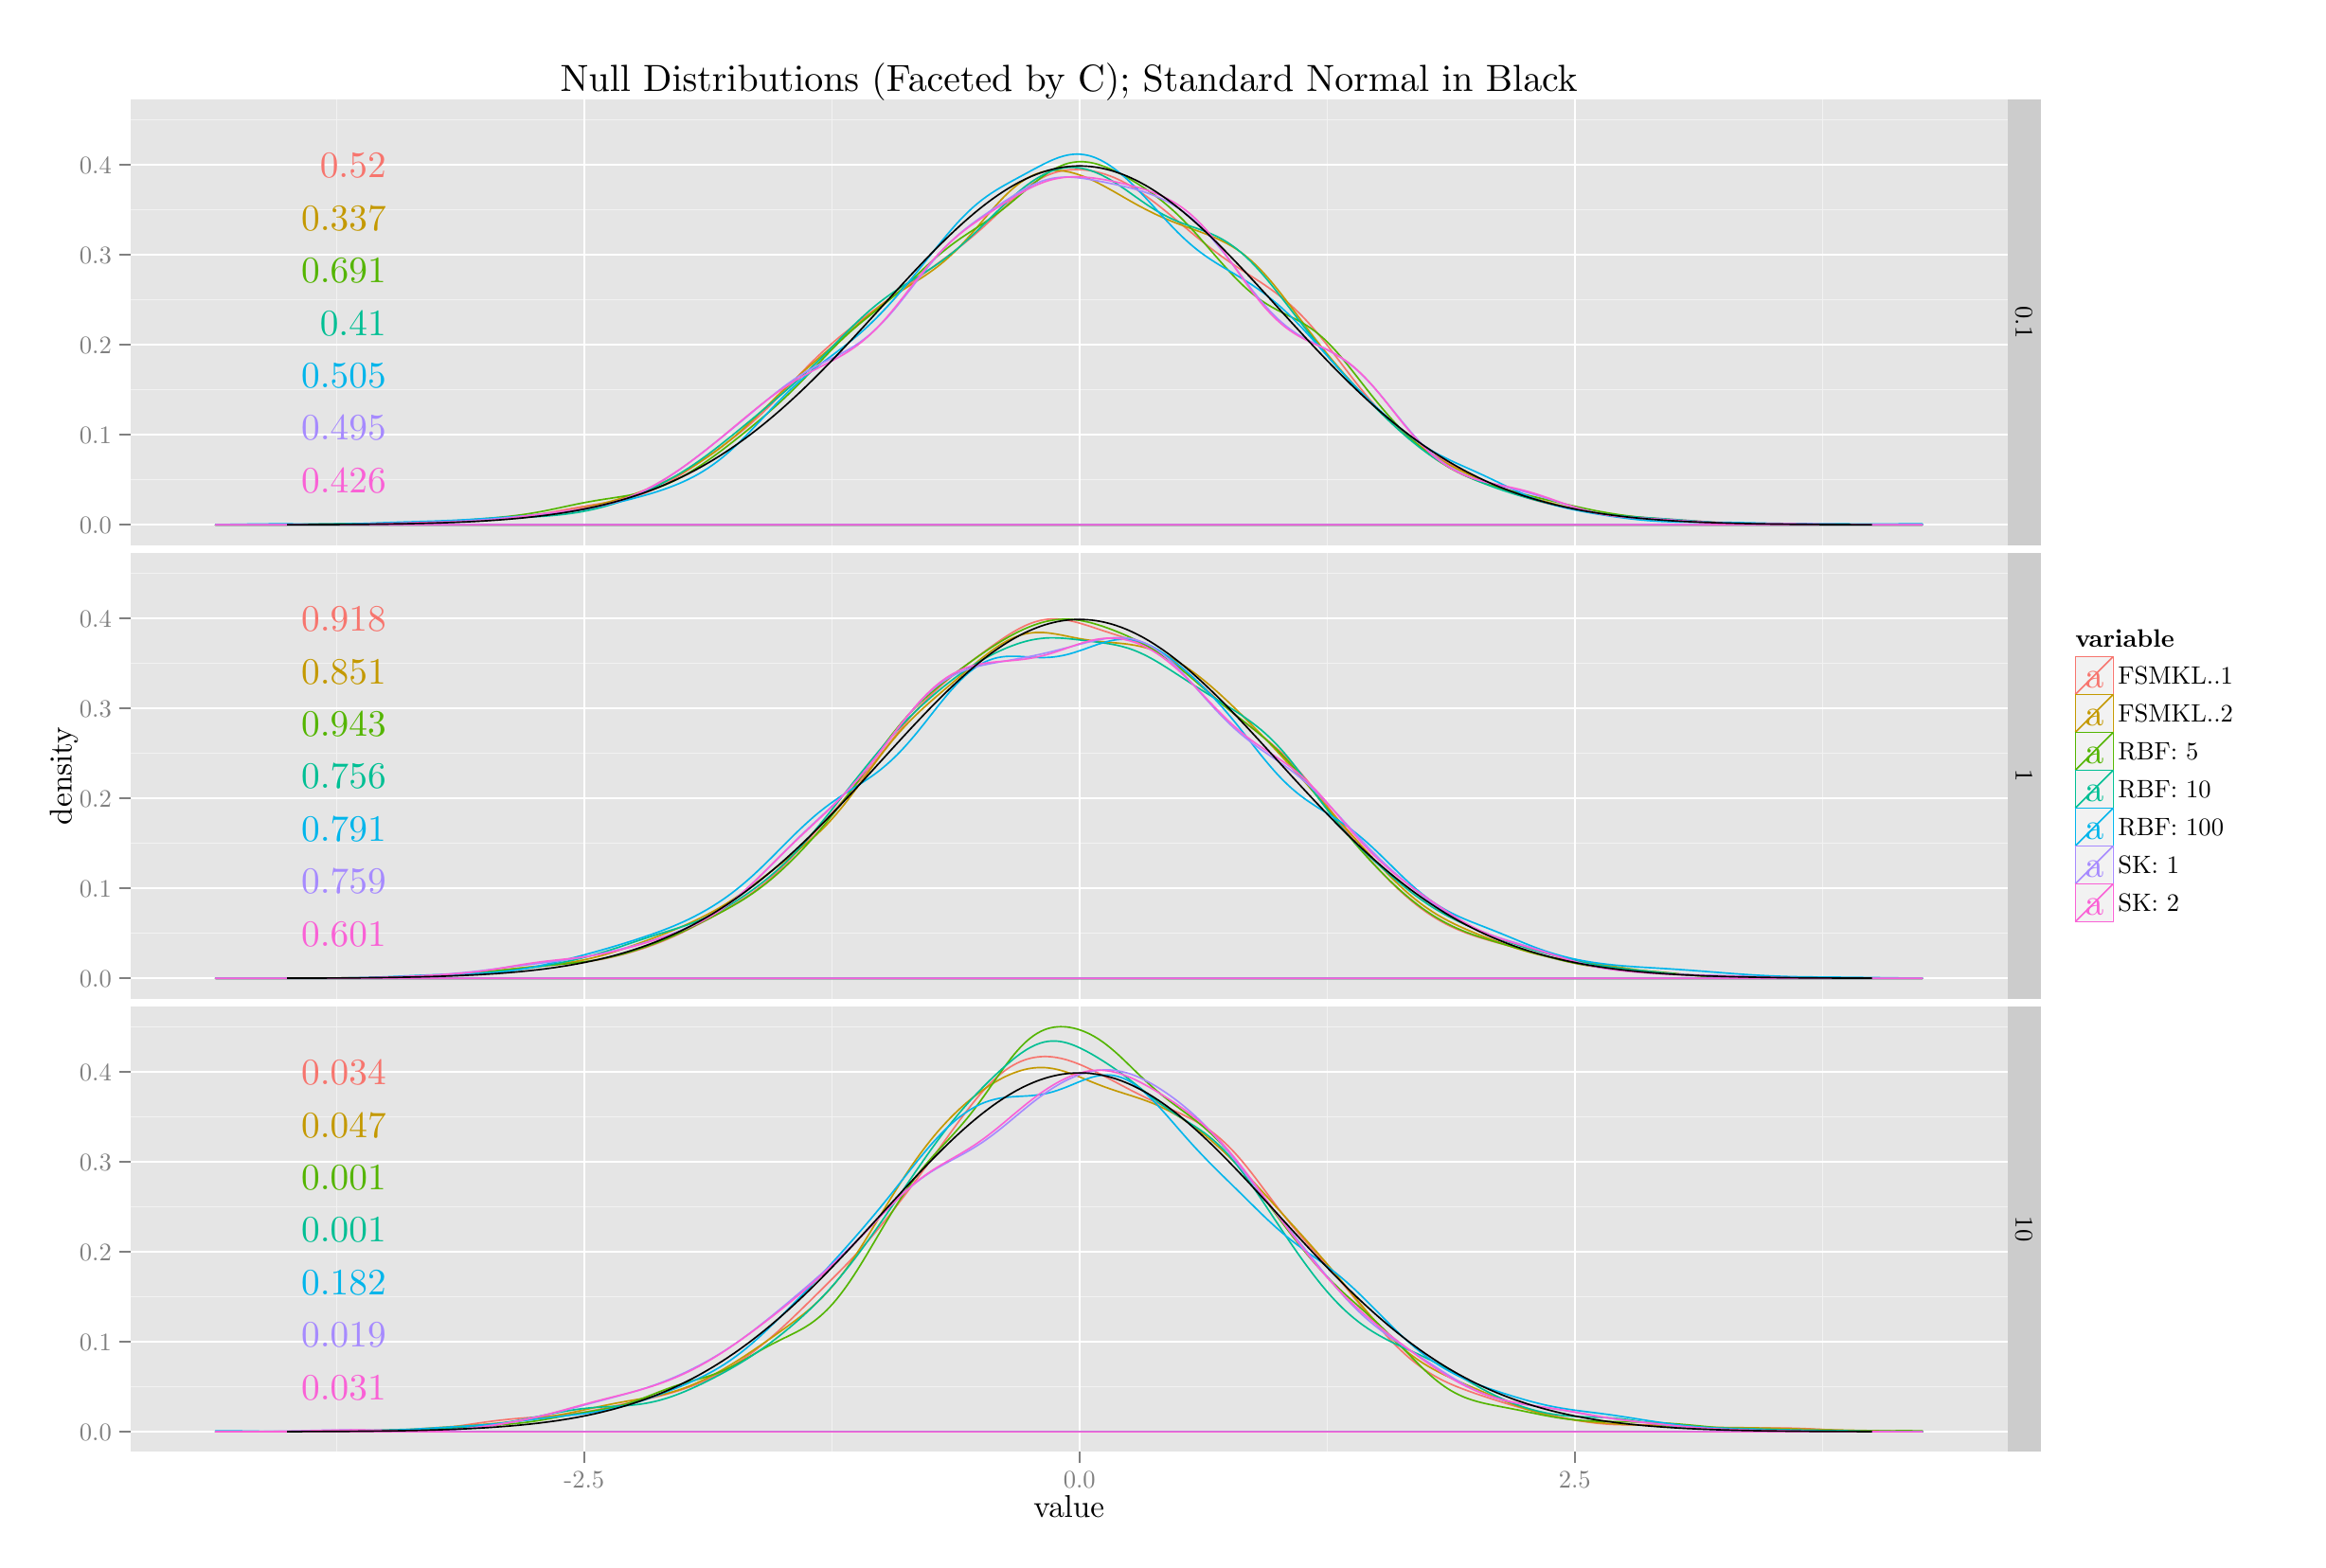
\begin{tikzpicture}[x=1pt,y=1pt]
\definecolor[named]{fillColor}{rgb}{1.00,1.00,1.00}
\path[use as bounding box,fill=fillColor,fill opacity=0.00] (0,0) rectangle (867.24,578.16);
\begin{scope}
\path[clip] (  0.00,  0.00) rectangle (867.24,578.16);
\definecolor[named]{drawColor}{rgb}{1.00,1.00,1.00}
\definecolor[named]{fillColor}{rgb}{1.00,1.00,1.00}

\path[draw=drawColor,line width= 0.6pt,line join=round,line cap=round,fill=fillColor] (  0.00, -0.00) rectangle (867.24,578.16);
\end{scope}
\begin{scope}
\path[clip] ( 39.69,380.14) rectangle (756.04,550.17);
\definecolor[named]{fillColor}{rgb}{0.90,0.90,0.90}

\path[fill=fillColor] ( 39.69,380.14) rectangle (756.04,550.17);
\definecolor[named]{drawColor}{rgb}{0.95,0.95,0.95}

\path[draw=drawColor,line width= 0.3pt,line join=round] ( 39.69,405.03) --
	(756.04,405.03);

\path[draw=drawColor,line width= 0.3pt,line join=round] ( 39.69,439.36) --
	(756.04,439.36);

\path[draw=drawColor,line width= 0.3pt,line join=round] ( 39.69,473.68) --
	(756.04,473.68);

\path[draw=drawColor,line width= 0.3pt,line join=round] ( 39.69,508.01) --
	(756.04,508.01);

\path[draw=drawColor,line width= 0.3pt,line join=round] ( 39.69,542.34) --
	(756.04,542.34);

\path[draw=drawColor,line width= 0.3pt,line join=round] (118.42,380.14) --
	(118.42,550.17);

\path[draw=drawColor,line width= 0.3pt,line join=round] (307.39,380.14) --
	(307.39,550.17);

\path[draw=drawColor,line width= 0.3pt,line join=round] (496.36,380.14) --
	(496.36,550.17);

\path[draw=drawColor,line width= 0.3pt,line join=round] (685.32,380.14) --
	(685.32,550.17);
\definecolor[named]{drawColor}{rgb}{1.00,1.00,1.00}

\path[draw=drawColor,line width= 0.6pt,line join=round] ( 39.69,387.86) --
	(756.04,387.86);

\path[draw=drawColor,line width= 0.6pt,line join=round] ( 39.69,422.19) --
	(756.04,422.19);

\path[draw=drawColor,line width= 0.6pt,line join=round] ( 39.69,456.52) --
	(756.04,456.52);

\path[draw=drawColor,line width= 0.6pt,line join=round] ( 39.69,490.85) --
	(756.04,490.85);

\path[draw=drawColor,line width= 0.6pt,line join=round] ( 39.69,525.18) --
	(756.04,525.18);

\path[draw=drawColor,line width= 0.6pt,line join=round] (212.90,380.14) --
	(212.90,550.17);

\path[draw=drawColor,line width= 0.6pt,line join=round] (401.87,380.14) --
	(401.87,550.17);

\path[draw=drawColor,line width= 0.6pt,line join=round] (590.84,380.14) --
	(590.84,550.17);
\definecolor[named]{drawColor}{rgb}{0.97,0.46,0.43}

\path[draw=drawColor,line width= 0.6pt,line join=round,line cap=round] ( 72.25,387.86) --
	( 73.52,387.86) --
	( 74.80,387.86) --
	( 76.07,387.86) --
	( 77.35,387.86) --
	( 78.62,387.86) --
	( 79.89,387.86) --
	( 81.17,387.86) --
	( 82.44,387.86) --
	( 83.72,387.86) --
	( 84.99,387.86) --
	( 86.27,387.86) --
	( 87.54,387.86) --
	( 88.82,387.86) --
	( 90.09,387.86) --
	( 91.36,387.87) --
	( 92.64,387.87) --
	( 93.91,387.87) --
	( 95.19,387.87) --
	( 96.46,387.87) --
	( 97.74,387.87) --
	( 99.01,387.87) --
	(100.29,387.87) --
	(101.56,387.87) --
	(102.83,387.87) --
	(104.11,387.87) --
	(105.38,387.87) --
	(106.66,387.87) --
	(107.93,387.88) --
	(109.21,387.88) --
	(110.48,387.88) --
	(111.76,387.89) --
	(113.03,387.89) --
	(114.30,387.90) --
	(115.58,387.90) --
	(116.85,387.91) --
	(118.13,387.92) --
	(119.40,387.93) --
	(120.68,387.94) --
	(121.95,387.96) --
	(123.22,387.97) --
	(124.50,387.99) --
	(125.77,388.01) --
	(127.05,388.03) --
	(128.32,388.06) --
	(129.60,388.08) --
	(130.87,388.11) --
	(132.15,388.14) --
	(133.42,388.17) --
	(134.69,388.21) --
	(135.97,388.24) --
	(137.24,388.28) --
	(138.52,388.33) --
	(139.79,388.37) --
	(141.07,388.42) --
	(142.34,388.47) --
	(143.62,388.52) --
	(144.89,388.57) --
	(146.16,388.63) --
	(147.44,388.68) --
	(148.71,388.74) --
	(149.99,388.80) --
	(151.26,388.86) --
	(152.54,388.93) --
	(153.81,388.99) --
	(155.09,389.05) --
	(156.36,389.12) --
	(157.63,389.18) --
	(158.91,389.25) --
	(160.18,389.31) --
	(161.46,389.37) --
	(162.73,389.44) --
	(164.01,389.50) --
	(165.28,389.55) --
	(166.56,389.61) --
	(167.83,389.67) --
	(169.10,389.72) --
	(170.38,389.77) --
	(171.65,389.82) --
	(172.93,389.87) --
	(174.20,389.92) --
	(175.48,389.98) --
	(176.75,390.03) --
	(178.03,390.09) --
	(179.30,390.16) --
	(180.57,390.23) --
	(181.85,390.30) --
	(183.12,390.39) --
	(184.40,390.49) --
	(185.67,390.59) --
	(186.95,390.71) --
	(188.22,390.84) --
	(189.49,390.98) --
	(190.77,391.14) --
	(192.04,391.30) --
	(193.32,391.48) --
	(194.59,391.68) --
	(195.87,391.88) --
	(197.14,392.09) --
	(198.42,392.31) --
	(199.69,392.54) --
	(200.96,392.77) --
	(202.24,393.01) --
	(203.51,393.25) --
	(204.79,393.49) --
	(206.06,393.72) --
	(207.34,393.96) --
	(208.61,394.20) --
	(209.89,394.42) --
	(211.16,394.65) --
	(212.43,394.87) --
	(213.71,395.09) --
	(214.98,395.30) --
	(216.26,395.51) --
	(217.53,395.71) --
	(218.81,395.92) --
	(220.08,396.13) --
	(221.36,396.34) --
	(222.63,396.56) --
	(223.90,396.79) --
	(225.18,397.03) --
	(226.45,397.29) --
	(227.73,397.56) --
	(229.00,397.86) --
	(230.28,398.18) --
	(231.55,398.52) --
	(232.83,398.89) --
	(234.10,399.30) --
	(235.37,399.74) --
	(236.65,400.21) --
	(237.92,400.72) --
	(239.20,401.26) --
	(240.47,401.83) --
	(241.75,402.44) --
	(243.02,403.08) --
	(244.29,403.76) --
	(245.57,404.46) --
	(246.84,405.20) --
	(248.12,405.95) --
	(249.39,406.74) --
	(250.67,407.54) --
	(251.94,408.37) --
	(253.22,409.21) --
	(254.49,410.06) --
	(255.76,410.93) --
	(257.04,411.81) --
	(258.31,412.69) --
	(259.59,413.59) --
	(260.86,414.49) --
	(262.14,415.40) --
	(263.41,416.32) --
	(264.69,417.24) --
	(265.96,418.17) --
	(267.23,419.12) --
	(268.51,420.08) --
	(269.78,421.06) --
	(271.06,422.05) --
	(272.33,423.06) --
	(273.61,424.10) --
	(274.88,425.16) --
	(276.16,426.25) --
	(277.43,427.37) --
	(278.70,428.51) --
	(279.98,429.69) --
	(281.25,430.90) --
	(282.53,432.13) --
	(283.80,433.39) --
	(285.08,434.68) --
	(286.35,435.99) --
	(287.63,437.32) --
	(288.90,438.66) --
	(290.17,440.00) --
	(291.45,441.36) --
	(292.72,442.71) --
	(294.00,444.06) --
	(295.27,445.40) --
	(296.55,446.72) --
	(297.82,448.03) --
	(299.10,449.32) --
	(300.37,450.58) --
	(301.64,451.81) --
	(302.92,453.02) --
	(304.19,454.20) --
	(305.47,455.36) --
	(306.74,456.49) --
	(308.02,457.60) --
	(309.29,458.68) --
	(310.56,459.75) --
	(311.84,460.79) --
	(313.11,461.82) --
	(314.39,462.84) --
	(315.66,463.84) --
	(316.94,464.84) --
	(318.21,465.82) --
	(319.49,466.80) --
	(320.76,467.77) --
	(322.03,468.74) --
	(323.31,469.71) --
	(324.58,470.66) --
	(325.86,471.62) --
	(327.13,472.57) --
	(328.41,473.51) --
	(329.68,474.46) --
	(330.96,475.40) --
	(332.23,476.33) --
	(333.50,477.26) --
	(334.78,478.19) --
	(336.05,479.12) --
	(337.33,480.05) --
	(338.60,480.97) --
	(339.88,481.89) --
	(341.15,482.81) --
	(342.43,483.73) --
	(343.70,484.65) --
	(344.97,485.57) --
	(346.25,486.50) --
	(347.52,487.43) --
	(348.80,488.36) --
	(350.07,489.30) --
	(351.35,490.24) --
	(352.62,491.20) --
	(353.90,492.16) --
	(355.17,493.14) --
	(356.44,494.14) --
	(357.72,495.15) --
	(358.99,496.19) --
	(360.27,497.24) --
	(361.54,498.32) --
	(362.82,499.42) --
	(364.09,500.54) --
	(365.37,501.68) --
	(366.64,502.85) --
	(367.91,504.03) --
	(369.19,505.23) --
	(370.46,506.43) --
	(371.74,507.64) --
	(373.01,508.85) --
	(374.29,510.05) --
	(375.56,511.23) --
	(376.83,512.39) --
	(378.11,513.52) --
	(379.38,514.61) --
	(380.66,515.65) --
	(381.93,516.65) --
	(383.21,517.58) --
	(384.48,518.44) --
	(385.76,519.24) --
	(387.03,519.98) --
	(388.30,520.64) --
	(389.58,521.24) --
	(390.85,521.74) --
	(392.13,522.18) --
	(393.40,522.55) --
	(394.68,522.85) --
	(395.95,523.09) --
	(397.23,523.27) --
	(398.50,523.39) --
	(399.77,523.44) --
	(401.05,523.45) --
	(402.32,523.40) --
	(403.60,523.31) --
	(404.87,523.17) --
	(406.15,522.98) --
	(407.42,522.74) --
	(408.70,522.46) --
	(409.97,522.14) --
	(411.24,521.77) --
	(412.52,521.35) --
	(413.79,520.89) --
	(415.07,520.39) --
	(416.34,519.83) --
	(417.62,519.23) --
	(418.89,518.58) --
	(420.17,517.89) --
	(421.44,517.16) --
	(422.71,516.39) --
	(423.99,515.58) --
	(425.26,514.73) --
	(426.54,513.85) --
	(427.81,512.93) --
	(429.09,511.99) --
	(430.36,511.03) --
	(431.63,510.04) --
	(432.91,509.03) --
	(434.18,508.01) --
	(435.46,506.97) --
	(436.73,505.92) --
	(438.01,504.86) --
	(439.28,503.80) --
	(440.56,502.73) --
	(441.83,501.66) --
	(443.10,500.60) --
	(444.38,499.54) --
	(445.65,498.48) --
	(446.93,497.43) --
	(448.20,496.40) --
	(449.48,495.38) --
	(450.75,494.37) --
	(452.03,493.38) --
	(453.30,492.40) --
	(454.57,491.45) --
	(455.85,490.51) --
	(457.12,489.60) --
	(458.40,488.70) --
	(459.67,487.82) --
	(460.95,486.96) --
	(462.22,486.11) --
	(463.50,485.27) --
	(464.77,484.45) --
	(466.04,483.63) --
	(467.32,482.81) --
	(468.59,481.99) --
	(469.87,481.16) --
	(471.14,480.32) --
	(472.42,479.47) --
	(473.69,478.60) --
	(474.97,477.70) --
	(476.24,476.77) --
	(477.51,475.81) --
	(478.79,474.82) --
	(480.06,473.79) --
	(481.34,472.70) --
	(482.61,471.58) --
	(483.89,470.40) --
	(485.16,469.18) --
	(486.44,467.92) --
	(487.71,466.60) --
	(488.98,465.23) --
	(490.26,463.81) --
	(491.53,462.34) --
	(492.81,460.84) --
	(494.08,459.29) --
	(495.36,457.72) --
	(496.63,456.11) --
	(497.90,454.47) --
	(499.18,452.81) --
	(500.45,451.14) --
	(501.73,449.47) --
	(503.00,447.79) --
	(504.28,446.12) --
	(505.55,444.46) --
	(506.83,442.81) --
	(508.10,441.19) --
	(509.37,439.60) --
	(510.65,438.03) --
	(511.92,436.50) --
	(513.20,435.00) --
	(514.47,433.55) --
	(515.75,432.14) --
	(517.02,430.77) --
	(518.30,429.45) --
	(519.57,428.17) --
	(520.84,426.93) --
	(522.12,425.74) --
	(523.39,424.60) --
	(524.67,423.49) --
	(525.94,422.43) --
	(527.22,421.40) --
	(528.49,420.41) --
	(529.77,419.46) --
	(531.04,418.55) --
	(532.31,417.66) --
	(533.59,416.81) --
	(534.86,415.98) --
	(536.14,415.18) --
	(537.41,414.40) --
	(538.69,413.65) --
	(539.96,412.91) --
	(541.24,412.19) --
	(542.51,411.48) --
	(543.78,410.79) --
	(545.06,410.11) --
	(546.33,409.45) --
	(547.61,408.79) --
	(548.88,408.15) --
	(550.16,407.51) --
	(551.43,406.88) --
	(552.71,406.26) --
	(553.98,405.65) --
	(555.25,405.05) --
	(556.53,404.46) --
	(557.80,403.89) --
	(559.08,403.32) --
	(560.35,402.77) --
	(561.63,402.23) --
	(562.90,401.70) --
	(564.17,401.19) --
	(565.45,400.70) --
	(566.72,400.22) --
	(568.00,399.75) --
	(569.27,399.30) --
	(570.55,398.87) --
	(571.82,398.45) --
	(573.10,398.05) --
	(574.37,397.66) --
	(575.64,397.29) --
	(576.92,396.93) --
	(578.19,396.58) --
	(579.47,396.25) --
	(580.74,395.94) --
	(582.02,395.63) --
	(583.29,395.34) --
	(584.57,395.06) --
	(585.84,394.79) --
	(587.11,394.54) --
	(588.39,394.29) --
	(589.66,394.05) --
	(590.94,393.83) --
	(592.21,393.61) --
	(593.49,393.40) --
	(594.76,393.20) --
	(596.04,393.01) --
	(597.31,392.82) --
	(598.58,392.64) --
	(599.86,392.47) --
	(601.13,392.30) --
	(602.41,392.14) --
	(603.68,391.98) --
	(604.96,391.83) --
	(606.23,391.69) --
	(607.51,391.55) --
	(608.78,391.41) --
	(610.05,391.28) --
	(611.33,391.16) --
	(612.60,391.04) --
	(613.88,390.93) --
	(615.15,390.82) --
	(616.43,390.72) --
	(617.70,390.62) --
	(618.97,390.52) --
	(620.25,390.43) --
	(621.52,390.34) --
	(622.80,390.26) --
	(624.07,390.17) --
	(625.35,390.09) --
	(626.62,390.01) --
	(627.90,389.93) --
	(629.17,389.84) --
	(630.44,389.76) --
	(631.72,389.68) --
	(632.99,389.60) --
	(634.27,389.51) --
	(635.54,389.43) --
	(636.82,389.34) --
	(638.09,389.26) --
	(639.37,389.17) --
	(640.64,389.08) --
	(641.91,389.00) --
	(643.19,388.92) --
	(644.46,388.83) --
	(645.74,388.75) --
	(647.01,388.68) --
	(648.29,388.60) --
	(649.56,388.53) --
	(650.84,388.46) --
	(652.11,388.40) --
	(653.38,388.34) --
	(654.66,388.28) --
	(655.93,388.23) --
	(657.21,388.19) --
	(658.48,388.14) --
	(659.76,388.10) --
	(661.03,388.07) --
	(662.31,388.04) --
	(663.58,388.01) --
	(664.85,387.99) --
	(666.13,387.97) --
	(667.40,387.95) --
	(668.68,387.94) --
	(669.95,387.92) --
	(671.23,387.91) --
	(672.50,387.90) --
	(673.78,387.90) --
	(675.05,387.89) --
	(676.32,387.88) --
	(677.60,387.88) --
	(678.87,387.88) --
	(680.15,387.87) --
	(681.42,387.87) --
	(682.70,387.87) --
	(683.97,387.87) --
	(685.24,387.87) --
	(686.52,387.87) --
	(687.79,387.87) --
	(689.07,387.87) --
	(690.34,387.87) --
	(691.62,387.87) --
	(692.89,387.87) --
	(694.17,387.87) --
	(695.44,387.86) --
	(696.71,387.86) --
	(697.99,387.86) --
	(699.26,387.86) --
	(700.54,387.86) --
	(701.81,387.86) --
	(703.09,387.86) --
	(704.36,387.86) --
	(705.64,387.86) --
	(706.91,387.86) --
	(708.18,387.86) --
	(709.46,387.86) --
	(710.73,387.86) --
	(712.01,387.86) --
	(713.28,387.86) --
	(714.56,387.86) --
	(715.83,387.86) --
	(717.11,387.86) --
	(718.38,387.86) --
	(719.65,387.86) --
	(720.93,387.86) --
	(722.20,387.86) --
	(723.48,387.86) --
	(723.48,387.86) --
	(722.20,387.86) --
	(720.93,387.86) --
	(719.65,387.86) --
	(718.38,387.86) --
	(717.11,387.86) --
	(715.83,387.86) --
	(714.56,387.86) --
	(713.28,387.86) --
	(712.01,387.86) --
	(710.73,387.86) --
	(709.46,387.86) --
	(708.18,387.86) --
	(706.91,387.86) --
	(705.64,387.86) --
	(704.36,387.86) --
	(703.09,387.86) --
	(701.81,387.86) --
	(700.54,387.86) --
	(699.26,387.86) --
	(697.99,387.86) --
	(696.71,387.86) --
	(695.44,387.86) --
	(694.17,387.86) --
	(692.89,387.86) --
	(691.62,387.86) --
	(690.34,387.86) --
	(689.07,387.86) --
	(687.79,387.86) --
	(686.52,387.86) --
	(685.24,387.86) --
	(683.97,387.86) --
	(682.70,387.86) --
	(681.42,387.86) --
	(680.15,387.86) --
	(678.87,387.86) --
	(677.60,387.86) --
	(676.32,387.86) --
	(675.05,387.86) --
	(673.78,387.86) --
	(672.50,387.86) --
	(671.23,387.86) --
	(669.95,387.86) --
	(668.68,387.86) --
	(667.40,387.86) --
	(666.13,387.86) --
	(664.85,387.86) --
	(663.58,387.86) --
	(662.31,387.86) --
	(661.03,387.86) --
	(659.76,387.86) --
	(658.48,387.86) --
	(657.21,387.86) --
	(655.93,387.86) --
	(654.66,387.86) --
	(653.38,387.86) --
	(652.11,387.86) --
	(650.84,387.86) --
	(649.56,387.86) --
	(648.29,387.86) --
	(647.01,387.86) --
	(645.74,387.86) --
	(644.46,387.86) --
	(643.19,387.86) --
	(641.91,387.86) --
	(640.64,387.86) --
	(639.37,387.86) --
	(638.09,387.86) --
	(636.82,387.86) --
	(635.54,387.86) --
	(634.27,387.86) --
	(632.99,387.86) --
	(631.72,387.86) --
	(630.44,387.86) --
	(629.17,387.86) --
	(627.90,387.86) --
	(626.62,387.86) --
	(625.35,387.86) --
	(624.07,387.86) --
	(622.80,387.86) --
	(621.52,387.86) --
	(620.25,387.86) --
	(618.97,387.86) --
	(617.70,387.86) --
	(616.43,387.86) --
	(615.15,387.86) --
	(613.88,387.86) --
	(612.60,387.86) --
	(611.33,387.86) --
	(610.05,387.86) --
	(608.78,387.86) --
	(607.51,387.86) --
	(606.23,387.86) --
	(604.96,387.86) --
	(603.68,387.86) --
	(602.41,387.86) --
	(601.13,387.86) --
	(599.86,387.86) --
	(598.58,387.86) --
	(597.31,387.86) --
	(596.04,387.86) --
	(594.76,387.86) --
	(593.49,387.86) --
	(592.21,387.86) --
	(590.94,387.86) --
	(589.66,387.86) --
	(588.39,387.86) --
	(587.11,387.86) --
	(585.84,387.86) --
	(584.57,387.86) --
	(583.29,387.86) --
	(582.02,387.86) --
	(580.74,387.86) --
	(579.47,387.86) --
	(578.19,387.86) --
	(576.92,387.86) --
	(575.64,387.86) --
	(574.37,387.86) --
	(573.10,387.86) --
	(571.82,387.86) --
	(570.55,387.86) --
	(569.27,387.86) --
	(568.00,387.86) --
	(566.72,387.86) --
	(565.45,387.86) --
	(564.17,387.86) --
	(562.90,387.86) --
	(561.63,387.86) --
	(560.35,387.86) --
	(559.08,387.86) --
	(557.80,387.86) --
	(556.53,387.86) --
	(555.25,387.86) --
	(553.98,387.86) --
	(552.71,387.86) --
	(551.43,387.86) --
	(550.16,387.86) --
	(548.88,387.86) --
	(547.61,387.86) --
	(546.33,387.86) --
	(545.06,387.86) --
	(543.78,387.86) --
	(542.51,387.86) --
	(541.24,387.86) --
	(539.96,387.86) --
	(538.69,387.86) --
	(537.41,387.86) --
	(536.14,387.86) --
	(534.86,387.86) --
	(533.59,387.86) --
	(532.31,387.86) --
	(531.04,387.86) --
	(529.77,387.86) --
	(528.49,387.86) --
	(527.22,387.86) --
	(525.94,387.86) --
	(524.67,387.86) --
	(523.39,387.86) --
	(522.12,387.86) --
	(520.84,387.86) --
	(519.57,387.86) --
	(518.30,387.86) --
	(517.02,387.86) --
	(515.75,387.86) --
	(514.47,387.86) --
	(513.20,387.86) --
	(511.92,387.86) --
	(510.65,387.86) --
	(509.37,387.86) --
	(508.10,387.86) --
	(506.83,387.86) --
	(505.55,387.86) --
	(504.28,387.86) --
	(503.00,387.86) --
	(501.73,387.86) --
	(500.45,387.86) --
	(499.18,387.86) --
	(497.90,387.86) --
	(496.63,387.86) --
	(495.36,387.86) --
	(494.08,387.86) --
	(492.81,387.86) --
	(491.53,387.86) --
	(490.26,387.86) --
	(488.98,387.86) --
	(487.71,387.86) --
	(486.44,387.86) --
	(485.16,387.86) --
	(483.89,387.86) --
	(482.61,387.86) --
	(481.34,387.86) --
	(480.06,387.86) --
	(478.79,387.86) --
	(477.51,387.86) --
	(476.24,387.86) --
	(474.97,387.86) --
	(473.69,387.86) --
	(472.42,387.86) --
	(471.14,387.86) --
	(469.87,387.86) --
	(468.59,387.86) --
	(467.32,387.86) --
	(466.04,387.86) --
	(464.77,387.86) --
	(463.50,387.86) --
	(462.22,387.86) --
	(460.95,387.86) --
	(459.67,387.86) --
	(458.40,387.86) --
	(457.12,387.86) --
	(455.85,387.86) --
	(454.57,387.86) --
	(453.30,387.86) --
	(452.03,387.86) --
	(450.75,387.86) --
	(449.48,387.86) --
	(448.20,387.86) --
	(446.93,387.86) --
	(445.65,387.86) --
	(444.38,387.86) --
	(443.10,387.86) --
	(441.83,387.86) --
	(440.56,387.86) --
	(439.28,387.86) --
	(438.01,387.86) --
	(436.73,387.86) --
	(435.46,387.86) --
	(434.18,387.86) --
	(432.91,387.86) --
	(431.63,387.86) --
	(430.36,387.86) --
	(429.09,387.86) --
	(427.81,387.86) --
	(426.54,387.86) --
	(425.26,387.86) --
	(423.99,387.86) --
	(422.71,387.86) --
	(421.44,387.86) --
	(420.17,387.86) --
	(418.89,387.86) --
	(417.62,387.86) --
	(416.34,387.86) --
	(415.07,387.86) --
	(413.79,387.86) --
	(412.52,387.86) --
	(411.24,387.86) --
	(409.97,387.86) --
	(408.70,387.86) --
	(407.42,387.86) --
	(406.15,387.86) --
	(404.87,387.86) --
	(403.60,387.86) --
	(402.32,387.86) --
	(401.05,387.86) --
	(399.77,387.86) --
	(398.50,387.86) --
	(397.23,387.86) --
	(395.95,387.86) --
	(394.68,387.86) --
	(393.40,387.86) --
	(392.13,387.86) --
	(390.85,387.86) --
	(389.58,387.86) --
	(388.30,387.86) --
	(387.03,387.86) --
	(385.76,387.86) --
	(384.48,387.86) --
	(383.21,387.86) --
	(381.93,387.86) --
	(380.66,387.86) --
	(379.38,387.86) --
	(378.11,387.86) --
	(376.83,387.86) --
	(375.56,387.86) --
	(374.29,387.86) --
	(373.01,387.86) --
	(371.74,387.86) --
	(370.46,387.86) --
	(369.19,387.86) --
	(367.91,387.86) --
	(366.64,387.86) --
	(365.37,387.86) --
	(364.09,387.86) --
	(362.82,387.86) --
	(361.54,387.86) --
	(360.27,387.86) --
	(358.99,387.86) --
	(357.72,387.86) --
	(356.44,387.86) --
	(355.17,387.86) --
	(353.90,387.86) --
	(352.62,387.86) --
	(351.35,387.86) --
	(350.07,387.86) --
	(348.80,387.86) --
	(347.52,387.86) --
	(346.25,387.86) --
	(344.97,387.86) --
	(343.70,387.86) --
	(342.43,387.86) --
	(341.15,387.86) --
	(339.88,387.86) --
	(338.60,387.86) --
	(337.33,387.86) --
	(336.05,387.86) --
	(334.78,387.86) --
	(333.50,387.86) --
	(332.23,387.86) --
	(330.96,387.86) --
	(329.68,387.86) --
	(328.41,387.86) --
	(327.13,387.86) --
	(325.86,387.86) --
	(324.58,387.86) --
	(323.31,387.86) --
	(322.03,387.86) --
	(320.76,387.86) --
	(319.49,387.86) --
	(318.21,387.86) --
	(316.94,387.86) --
	(315.66,387.86) --
	(314.39,387.86) --
	(313.11,387.86) --
	(311.84,387.86) --
	(310.56,387.86) --
	(309.29,387.86) --
	(308.02,387.86) --
	(306.74,387.86) --
	(305.47,387.86) --
	(304.19,387.86) --
	(302.92,387.86) --
	(301.64,387.86) --
	(300.37,387.86) --
	(299.10,387.86) --
	(297.82,387.86) --
	(296.55,387.86) --
	(295.27,387.86) --
	(294.00,387.86) --
	(292.72,387.86) --
	(291.45,387.86) --
	(290.17,387.86) --
	(288.90,387.86) --
	(287.63,387.86) --
	(286.35,387.86) --
	(285.08,387.86) --
	(283.80,387.86) --
	(282.53,387.86) --
	(281.25,387.86) --
	(279.98,387.86) --
	(278.70,387.86) --
	(277.43,387.86) --
	(276.16,387.86) --
	(274.88,387.86) --
	(273.61,387.86) --
	(272.33,387.86) --
	(271.06,387.86) --
	(269.78,387.86) --
	(268.51,387.86) --
	(267.23,387.86) --
	(265.96,387.86) --
	(264.69,387.86) --
	(263.41,387.86) --
	(262.14,387.86) --
	(260.86,387.86) --
	(259.59,387.86) --
	(258.31,387.86) --
	(257.04,387.86) --
	(255.76,387.86) --
	(254.49,387.86) --
	(253.22,387.86) --
	(251.94,387.86) --
	(250.67,387.86) --
	(249.39,387.86) --
	(248.12,387.86) --
	(246.84,387.86) --
	(245.57,387.86) --
	(244.29,387.86) --
	(243.02,387.86) --
	(241.75,387.86) --
	(240.47,387.86) --
	(239.20,387.86) --
	(237.92,387.86) --
	(236.65,387.86) --
	(235.37,387.86) --
	(234.10,387.86) --
	(232.83,387.86) --
	(231.55,387.86) --
	(230.28,387.86) --
	(229.00,387.86) --
	(227.73,387.86) --
	(226.45,387.86) --
	(225.18,387.86) --
	(223.90,387.86) --
	(222.63,387.86) --
	(221.36,387.86) --
	(220.08,387.86) --
	(218.81,387.86) --
	(217.53,387.86) --
	(216.26,387.86) --
	(214.98,387.86) --
	(213.71,387.86) --
	(212.43,387.86) --
	(211.16,387.86) --
	(209.89,387.86) --
	(208.61,387.86) --
	(207.34,387.86) --
	(206.06,387.86) --
	(204.79,387.86) --
	(203.51,387.86) --
	(202.24,387.86) --
	(200.96,387.86) --
	(199.69,387.86) --
	(198.42,387.86) --
	(197.14,387.86) --
	(195.87,387.86) --
	(194.59,387.86) --
	(193.32,387.86) --
	(192.04,387.86) --
	(190.77,387.86) --
	(189.49,387.86) --
	(188.22,387.86) --
	(186.95,387.86) --
	(185.67,387.86) --
	(184.40,387.86) --
	(183.12,387.86) --
	(181.85,387.86) --
	(180.57,387.86) --
	(179.30,387.86) --
	(178.03,387.86) --
	(176.75,387.86) --
	(175.48,387.86) --
	(174.20,387.86) --
	(172.93,387.86) --
	(171.65,387.86) --
	(170.38,387.86) --
	(169.10,387.86) --
	(167.83,387.86) --
	(166.56,387.86) --
	(165.28,387.86) --
	(164.01,387.86) --
	(162.73,387.86) --
	(161.46,387.86) --
	(160.18,387.86) --
	(158.91,387.86) --
	(157.63,387.86) --
	(156.36,387.86) --
	(155.09,387.86) --
	(153.81,387.86) --
	(152.54,387.86) --
	(151.26,387.86) --
	(149.99,387.86) --
	(148.71,387.86) --
	(147.44,387.86) --
	(146.16,387.86) --
	(144.89,387.86) --
	(143.62,387.86) --
	(142.34,387.86) --
	(141.07,387.86) --
	(139.79,387.86) --
	(138.52,387.86) --
	(137.24,387.86) --
	(135.97,387.86) --
	(134.69,387.86) --
	(133.42,387.86) --
	(132.15,387.86) --
	(130.87,387.86) --
	(129.60,387.86) --
	(128.32,387.86) --
	(127.05,387.86) --
	(125.77,387.86) --
	(124.50,387.86) --
	(123.22,387.86) --
	(121.95,387.86) --
	(120.68,387.86) --
	(119.40,387.86) --
	(118.13,387.86) --
	(116.85,387.86) --
	(115.58,387.86) --
	(114.30,387.86) --
	(113.03,387.86) --
	(111.76,387.86) --
	(110.48,387.86) --
	(109.21,387.86) --
	(107.93,387.86) --
	(106.66,387.86) --
	(105.38,387.86) --
	(104.11,387.86) --
	(102.83,387.86) --
	(101.56,387.86) --
	(100.29,387.86) --
	( 99.01,387.86) --
	( 97.74,387.86) --
	( 96.46,387.86) --
	( 95.19,387.86) --
	( 93.91,387.86) --
	( 92.64,387.86) --
	( 91.36,387.86) --
	( 90.09,387.86) --
	( 88.82,387.86) --
	( 87.54,387.86) --
	( 86.27,387.86) --
	( 84.99,387.86) --
	( 83.72,387.86) --
	( 82.44,387.86) --
	( 81.17,387.86) --
	( 79.89,387.86) --
	( 78.62,387.86) --
	( 77.35,387.86) --
	( 76.07,387.86) --
	( 74.80,387.86) --
	( 73.52,387.86) --
	( 72.25,387.86) --
	( 72.25,387.86);
\definecolor[named]{drawColor}{rgb}{0.77,0.60,0.00}

\path[draw=drawColor,line width= 0.6pt,line join=round,line cap=round] ( 72.25,387.87) --
	( 73.52,387.87) --
	( 74.80,387.87) --
	( 76.07,387.87) --
	( 77.35,387.87) --
	( 78.62,387.87) --
	( 79.89,387.87) --
	( 81.17,387.87) --
	( 82.44,387.87) --
	( 83.72,387.87) --
	( 84.99,387.88) --
	( 86.27,387.88) --
	( 87.54,387.88) --
	( 88.82,387.89) --
	( 90.09,387.89) --
	( 91.36,387.90) --
	( 92.64,387.91) --
	( 93.91,387.91) --
	( 95.19,387.92) --
	( 96.46,387.93) --
	( 97.74,387.94) --
	( 99.01,387.96) --
	(100.29,387.97) --
	(101.56,387.98) --
	(102.83,388.00) --
	(104.11,388.02) --
	(105.38,388.03) --
	(106.66,388.05) --
	(107.93,388.07) --
	(109.21,388.09) --
	(110.48,388.11) --
	(111.76,388.12) --
	(113.03,388.14) --
	(114.30,388.16) --
	(115.58,388.18) --
	(116.85,388.19) --
	(118.13,388.20) --
	(119.40,388.22) --
	(120.68,388.23) --
	(121.95,388.23) --
	(123.22,388.24) --
	(124.50,388.25) --
	(125.77,388.25) --
	(127.05,388.25) --
	(128.32,388.26) --
	(129.60,388.26) --
	(130.87,388.26) --
	(132.15,388.26) --
	(133.42,388.26) --
	(134.69,388.26) --
	(135.97,388.26) --
	(137.24,388.27) --
	(138.52,388.28) --
	(139.79,388.28) --
	(141.07,388.30) --
	(142.34,388.31) --
	(143.62,388.33) --
	(144.89,388.35) --
	(146.16,388.37) --
	(147.44,388.40) --
	(148.71,388.43) --
	(149.99,388.46) --
	(151.26,388.50) --
	(152.54,388.54) --
	(153.81,388.58) --
	(155.09,388.63) --
	(156.36,388.68) --
	(157.63,388.74) --
	(158.91,388.80) --
	(160.18,388.86) --
	(161.46,388.93) --
	(162.73,389.00) --
	(164.01,389.08) --
	(165.28,389.15) --
	(166.56,389.23) --
	(167.83,389.32) --
	(169.10,389.40) --
	(170.38,389.49) --
	(171.65,389.58) --
	(172.93,389.68) --
	(174.20,389.77) --
	(175.48,389.87) --
	(176.75,389.97) --
	(178.03,390.08) --
	(179.30,390.18) --
	(180.57,390.29) --
	(181.85,390.40) --
	(183.12,390.51) --
	(184.40,390.62) --
	(185.67,390.74) --
	(186.95,390.86) --
	(188.22,390.99) --
	(189.49,391.11) --
	(190.77,391.24) --
	(192.04,391.38) --
	(193.32,391.52) --
	(194.59,391.66) --
	(195.87,391.81) --
	(197.14,391.97) --
	(198.42,392.12) --
	(199.69,392.29) --
	(200.96,392.46) --
	(202.24,392.64) --
	(203.51,392.82) --
	(204.79,393.01) --
	(206.06,393.21) --
	(207.34,393.42) --
	(208.61,393.64) --
	(209.89,393.86) --
	(211.16,394.10) --
	(212.43,394.35) --
	(213.71,394.60) --
	(214.98,394.87) --
	(216.26,395.15) --
	(217.53,395.44) --
	(218.81,395.74) --
	(220.08,396.06) --
	(221.36,396.38) --
	(222.63,396.72) --
	(223.90,397.07) --
	(225.18,397.44) --
	(226.45,397.82) --
	(227.73,398.21) --
	(229.00,398.61) --
	(230.28,399.03) --
	(231.55,399.46) --
	(232.83,399.91) --
	(234.10,400.37) --
	(235.37,400.85) --
	(236.65,401.34) --
	(237.92,401.85) --
	(239.20,402.38) --
	(240.47,402.93) --
	(241.75,403.49) --
	(243.02,404.08) --
	(244.29,404.68) --
	(245.57,405.31) --
	(246.84,405.95) --
	(248.12,406.61) --
	(249.39,407.29) --
	(250.67,407.99) --
	(251.94,408.72) --
	(253.22,409.46) --
	(254.49,410.23) --
	(255.76,411.01) --
	(257.04,411.82) --
	(258.31,412.64) --
	(259.59,413.50) --
	(260.86,414.37) --
	(262.14,415.27) --
	(263.41,416.19) --
	(264.69,417.14) --
	(265.96,418.12) --
	(267.23,419.12) --
	(268.51,420.16) --
	(269.78,421.22) --
	(271.06,422.31) --
	(272.33,423.42) --
	(273.61,424.56) --
	(274.88,425.73) --
	(276.16,426.92) --
	(277.43,428.13) --
	(278.70,429.35) --
	(279.98,430.59) --
	(281.25,431.83) --
	(282.53,433.08) --
	(283.80,434.34) --
	(285.08,435.59) --
	(286.35,436.84) --
	(287.63,438.08) --
	(288.90,439.30) --
	(290.17,440.52) --
	(291.45,441.72) --
	(292.72,442.91) --
	(294.00,444.08) --
	(295.27,445.23) --
	(296.55,446.37) --
	(297.82,447.50) --
	(299.10,448.62) --
	(300.37,449.73) --
	(301.64,450.83) --
	(302.92,451.93) --
	(304.19,453.02) --
	(305.47,454.12) --
	(306.74,455.21) --
	(308.02,456.31) --
	(309.29,457.41) --
	(310.56,458.51) --
	(311.84,459.62) --
	(313.11,460.72) --
	(314.39,461.83) --
	(315.66,462.94) --
	(316.94,464.04) --
	(318.21,465.13) --
	(319.49,466.21) --
	(320.76,467.28) --
	(322.03,468.34) --
	(323.31,469.38) --
	(324.58,470.40) --
	(325.86,471.40) --
	(327.13,472.37) --
	(328.41,473.32) --
	(329.68,474.24) --
	(330.96,475.14) --
	(332.23,476.02) --
	(333.50,476.87) --
	(334.78,477.71) --
	(336.05,478.54) --
	(337.33,479.35) --
	(338.60,480.17) --
	(339.88,480.98) --
	(341.15,481.80) --
	(342.43,482.64) --
	(343.70,483.50) --
	(344.97,484.38) --
	(346.25,485.30) --
	(347.52,486.25) --
	(348.80,487.25) --
	(350.07,488.31) --
	(351.35,489.41) --
	(352.62,490.56) --
	(353.90,491.76) --
	(355.17,493.02) --
	(356.44,494.32) --
	(357.72,495.68) --
	(358.99,497.07) --
	(360.27,498.51) --
	(361.54,499.97) --
	(362.82,501.45) --
	(364.09,502.94) --
	(365.37,504.44) --
	(366.64,505.93) --
	(367.91,507.40) --
	(369.19,508.85) --
	(370.46,510.26) --
	(371.74,511.64) --
	(373.01,512.96) --
	(374.29,514.21) --
	(375.56,515.40) --
	(376.83,516.51) --
	(378.11,517.55) --
	(379.38,518.50) --
	(380.66,519.37) --
	(381.93,520.15) --
	(383.21,520.83) --
	(384.48,521.42) --
	(385.76,521.92) --
	(387.03,522.33) --
	(388.30,522.65) --
	(389.58,522.90) --
	(390.85,523.04) --
	(392.13,523.10) --
	(393.40,523.10) --
	(394.68,523.02) --
	(395.95,522.87) --
	(397.23,522.66) --
	(398.50,522.39) --
	(399.77,522.05) --
	(401.05,521.66) --
	(402.32,521.23) --
	(403.60,520.75) --
	(404.87,520.23) --
	(406.15,519.67) --
	(407.42,519.08) --
	(408.70,518.45) --
	(409.97,517.80) --
	(411.24,517.12) --
	(412.52,516.43) --
	(413.79,515.72) --
	(415.07,515.00) --
	(416.34,514.27) --
	(417.62,513.54) --
	(418.89,512.80) --
	(420.17,512.07) --
	(421.44,511.34) --
	(422.71,510.63) --
	(423.99,509.92) --
	(425.26,509.23) --
	(426.54,508.56) --
	(427.81,507.90) --
	(429.09,507.26) --
	(430.36,506.64) --
	(431.63,506.04) --
	(432.91,505.47) --
	(434.18,504.91) --
	(435.46,504.37) --
	(436.73,503.84) --
	(438.01,503.33) --
	(439.28,502.84) --
	(440.56,502.35) --
	(441.83,501.88) --
	(443.10,501.41) --
	(444.38,500.95) --
	(445.65,500.49) --
	(446.93,500.03) --
	(448.20,499.56) --
	(449.48,499.08) --
	(450.75,498.58) --
	(452.03,498.07) --
	(453.30,497.54) --
	(454.57,496.98) --
	(455.85,496.39) --
	(457.12,495.76) --
	(458.40,495.08) --
	(459.67,494.35) --
	(460.95,493.58) --
	(462.22,492.74) --
	(463.50,491.85) --
	(464.77,490.88) --
	(466.04,489.84) --
	(467.32,488.74) --
	(468.59,487.57) --
	(469.87,486.33) --
	(471.14,485.03) --
	(472.42,483.66) --
	(473.69,482.22) --
	(474.97,480.73) --
	(476.24,479.20) --
	(477.51,477.62) --
	(478.79,476.00) --
	(480.06,474.36) --
	(481.34,472.68) --
	(482.61,471.00) --
	(483.89,469.30) --
	(485.16,467.60) --
	(486.44,465.90) --
	(487.71,464.20) --
	(488.98,462.51) --
	(490.26,460.84) --
	(491.53,459.19) --
	(492.81,457.56) --
	(494.08,455.94) --
	(495.36,454.35) --
	(496.63,452.78) --
	(497.90,451.23) --
	(499.18,449.72) --
	(500.45,448.22) --
	(501.73,446.74) --
	(503.00,445.29) --
	(504.28,443.86) --
	(505.55,442.46) --
	(506.83,441.07) --
	(508.10,439.71) --
	(509.37,438.37) --
	(510.65,437.04) --
	(511.92,435.73) --
	(513.20,434.44) --
	(514.47,433.18) --
	(515.75,431.93) --
	(517.02,430.69) --
	(518.30,429.48) --
	(519.57,428.28) --
	(520.84,427.11) --
	(522.12,425.95) --
	(523.39,424.82) --
	(524.67,423.71) --
	(525.94,422.62) --
	(527.22,421.55) --
	(528.49,420.51) --
	(529.77,419.50) --
	(531.04,418.52) --
	(532.31,417.56) --
	(533.59,416.64) --
	(534.86,415.75) --
	(536.14,414.88) --
	(537.41,414.05) --
	(538.69,413.25) --
	(539.96,412.47) --
	(541.24,411.73) --
	(542.51,411.01) --
	(543.78,410.32) --
	(545.06,409.65) --
	(546.33,409.00) --
	(547.61,408.38) --
	(548.88,407.77) --
	(550.16,407.18) --
	(551.43,406.61) --
	(552.71,406.05) --
	(553.98,405.51) --
	(555.25,404.98) --
	(556.53,404.46) --
	(557.80,403.95) --
	(559.08,403.46) --
	(560.35,402.98) --
	(561.63,402.50) --
	(562.90,402.04) --
	(564.17,401.59) --
	(565.45,401.15) --
	(566.72,400.72) --
	(568.00,400.30) --
	(569.27,399.88) --
	(570.55,399.48) --
	(571.82,399.08) --
	(573.10,398.69) --
	(574.37,398.30) --
	(575.64,397.93) --
	(576.92,397.55) --
	(578.19,397.19) --
	(579.47,396.83) --
	(580.74,396.48) --
	(582.02,396.13) --
	(583.29,395.79) --
	(584.57,395.45) --
	(585.84,395.13) --
	(587.11,394.81) --
	(588.39,394.51) --
	(589.66,394.21) --
	(590.94,393.92) --
	(592.21,393.65) --
	(593.49,393.38) --
	(594.76,393.13) --
	(596.04,392.89) --
	(597.31,392.67) --
	(598.58,392.46) --
	(599.86,392.25) --
	(601.13,392.06) --
	(602.41,391.89) --
	(603.68,391.72) --
	(604.96,391.56) --
	(606.23,391.42) --
	(607.51,391.28) --
	(608.78,391.15) --
	(610.05,391.03) --
	(611.33,390.92) --
	(612.60,390.81) --
	(613.88,390.71) --
	(615.15,390.61) --
	(616.43,390.52) --
	(617.70,390.43) --
	(618.97,390.33) --
	(620.25,390.25) --
	(621.52,390.16) --
	(622.80,390.07) --
	(624.07,389.98) --
	(625.35,389.88) --
	(626.62,389.79) --
	(627.90,389.70) --
	(629.17,389.60) --
	(630.44,389.51) --
	(631.72,389.41) --
	(632.99,389.31) --
	(634.27,389.21) --
	(635.54,389.12) --
	(636.82,389.02) --
	(638.09,388.92) --
	(639.37,388.83) --
	(640.64,388.74) --
	(641.91,388.66) --
	(643.19,388.58) --
	(644.46,388.50) --
	(645.74,388.43) --
	(647.01,388.36) --
	(648.29,388.30) --
	(649.56,388.24) --
	(650.84,388.19) --
	(652.11,388.15) --
	(653.38,388.10) --
	(654.66,388.07) --
	(655.93,388.04) --
	(657.21,388.01) --
	(658.48,387.98) --
	(659.76,387.96) --
	(661.03,387.94) --
	(662.31,387.93) --
	(663.58,387.92) --
	(664.85,387.91) --
	(666.13,387.90) --
	(667.40,387.89) --
	(668.68,387.89) --
	(669.95,387.88) --
	(671.23,387.88) --
	(672.50,387.87) --
	(673.78,387.87) --
	(675.05,387.87) --
	(676.32,387.87) --
	(677.60,387.87) --
	(678.87,387.87) --
	(680.15,387.87) --
	(681.42,387.87) --
	(682.70,387.87) --
	(683.97,387.87) --
	(685.24,387.87) --
	(686.52,387.87) --
	(687.79,387.86) --
	(689.07,387.86) --
	(690.34,387.86) --
	(691.62,387.86) --
	(692.89,387.86) --
	(694.17,387.86) --
	(695.44,387.86) --
	(696.71,387.86) --
	(697.99,387.86) --
	(699.26,387.86) --
	(700.54,387.86) --
	(701.81,387.86) --
	(703.09,387.86) --
	(704.36,387.86) --
	(705.64,387.86) --
	(706.91,387.86) --
	(708.18,387.86) --
	(709.46,387.86) --
	(710.73,387.86) --
	(712.01,387.86) --
	(713.28,387.86) --
	(714.56,387.86) --
	(715.83,387.86) --
	(717.11,387.86) --
	(718.38,387.86) --
	(719.65,387.86) --
	(720.93,387.86) --
	(722.20,387.86) --
	(723.48,387.86) --
	(723.48,387.86) --
	(722.20,387.86) --
	(720.93,387.86) --
	(719.65,387.86) --
	(718.38,387.86) --
	(717.11,387.86) --
	(715.83,387.86) --
	(714.56,387.86) --
	(713.28,387.86) --
	(712.01,387.86) --
	(710.73,387.86) --
	(709.46,387.86) --
	(708.18,387.86) --
	(706.91,387.86) --
	(705.64,387.86) --
	(704.36,387.86) --
	(703.09,387.86) --
	(701.81,387.86) --
	(700.54,387.86) --
	(699.26,387.86) --
	(697.99,387.86) --
	(696.71,387.86) --
	(695.44,387.86) --
	(694.17,387.86) --
	(692.89,387.86) --
	(691.62,387.86) --
	(690.34,387.86) --
	(689.07,387.86) --
	(687.79,387.86) --
	(686.52,387.86) --
	(685.24,387.86) --
	(683.97,387.86) --
	(682.70,387.86) --
	(681.42,387.86) --
	(680.15,387.86) --
	(678.87,387.86) --
	(677.60,387.86) --
	(676.32,387.86) --
	(675.05,387.86) --
	(673.78,387.86) --
	(672.50,387.86) --
	(671.23,387.86) --
	(669.95,387.86) --
	(668.68,387.86) --
	(667.40,387.86) --
	(666.13,387.86) --
	(664.85,387.86) --
	(663.58,387.86) --
	(662.31,387.86) --
	(661.03,387.86) --
	(659.76,387.86) --
	(658.48,387.86) --
	(657.21,387.86) --
	(655.93,387.86) --
	(654.66,387.86) --
	(653.38,387.86) --
	(652.11,387.86) --
	(650.84,387.86) --
	(649.56,387.86) --
	(648.29,387.86) --
	(647.01,387.86) --
	(645.74,387.86) --
	(644.46,387.86) --
	(643.19,387.86) --
	(641.91,387.86) --
	(640.64,387.86) --
	(639.37,387.86) --
	(638.09,387.86) --
	(636.82,387.86) --
	(635.54,387.86) --
	(634.27,387.86) --
	(632.99,387.86) --
	(631.72,387.86) --
	(630.44,387.86) --
	(629.17,387.86) --
	(627.90,387.86) --
	(626.62,387.86) --
	(625.35,387.86) --
	(624.07,387.86) --
	(622.80,387.86) --
	(621.52,387.86) --
	(620.25,387.86) --
	(618.97,387.86) --
	(617.70,387.86) --
	(616.43,387.86) --
	(615.15,387.86) --
	(613.88,387.86) --
	(612.60,387.86) --
	(611.33,387.86) --
	(610.05,387.86) --
	(608.78,387.86) --
	(607.51,387.86) --
	(606.23,387.86) --
	(604.96,387.86) --
	(603.68,387.86) --
	(602.41,387.86) --
	(601.13,387.86) --
	(599.86,387.86) --
	(598.58,387.86) --
	(597.31,387.86) --
	(596.04,387.86) --
	(594.76,387.86) --
	(593.49,387.86) --
	(592.21,387.86) --
	(590.94,387.86) --
	(589.66,387.86) --
	(588.39,387.86) --
	(587.11,387.86) --
	(585.84,387.86) --
	(584.57,387.86) --
	(583.29,387.86) --
	(582.02,387.86) --
	(580.74,387.86) --
	(579.47,387.86) --
	(578.19,387.86) --
	(576.92,387.86) --
	(575.64,387.86) --
	(574.37,387.86) --
	(573.10,387.86) --
	(571.82,387.86) --
	(570.55,387.86) --
	(569.27,387.86) --
	(568.00,387.86) --
	(566.72,387.86) --
	(565.45,387.86) --
	(564.17,387.86) --
	(562.90,387.86) --
	(561.63,387.86) --
	(560.35,387.86) --
	(559.08,387.86) --
	(557.80,387.86) --
	(556.53,387.86) --
	(555.25,387.86) --
	(553.98,387.86) --
	(552.71,387.86) --
	(551.43,387.86) --
	(550.16,387.86) --
	(548.88,387.86) --
	(547.61,387.86) --
	(546.33,387.86) --
	(545.06,387.86) --
	(543.78,387.86) --
	(542.51,387.86) --
	(541.24,387.86) --
	(539.96,387.86) --
	(538.69,387.86) --
	(537.41,387.86) --
	(536.14,387.86) --
	(534.86,387.86) --
	(533.59,387.86) --
	(532.31,387.86) --
	(531.04,387.86) --
	(529.77,387.86) --
	(528.49,387.86) --
	(527.22,387.86) --
	(525.94,387.86) --
	(524.67,387.86) --
	(523.39,387.86) --
	(522.12,387.86) --
	(520.84,387.86) --
	(519.57,387.86) --
	(518.30,387.86) --
	(517.02,387.86) --
	(515.75,387.86) --
	(514.47,387.86) --
	(513.20,387.86) --
	(511.92,387.86) --
	(510.65,387.86) --
	(509.37,387.86) --
	(508.10,387.86) --
	(506.83,387.86) --
	(505.55,387.86) --
	(504.28,387.86) --
	(503.00,387.86) --
	(501.73,387.86) --
	(500.45,387.86) --
	(499.18,387.86) --
	(497.90,387.86) --
	(496.63,387.86) --
	(495.36,387.86) --
	(494.08,387.86) --
	(492.81,387.86) --
	(491.53,387.86) --
	(490.26,387.86) --
	(488.98,387.86) --
	(487.71,387.86) --
	(486.44,387.86) --
	(485.16,387.86) --
	(483.89,387.86) --
	(482.61,387.86) --
	(481.34,387.86) --
	(480.06,387.86) --
	(478.79,387.86) --
	(477.51,387.86) --
	(476.24,387.86) --
	(474.97,387.86) --
	(473.69,387.86) --
	(472.42,387.86) --
	(471.14,387.86) --
	(469.87,387.86) --
	(468.59,387.86) --
	(467.32,387.86) --
	(466.04,387.86) --
	(464.77,387.86) --
	(463.50,387.86) --
	(462.22,387.86) --
	(460.95,387.86) --
	(459.67,387.86) --
	(458.40,387.86) --
	(457.12,387.86) --
	(455.85,387.86) --
	(454.57,387.86) --
	(453.30,387.86) --
	(452.03,387.86) --
	(450.75,387.86) --
	(449.48,387.86) --
	(448.20,387.86) --
	(446.93,387.86) --
	(445.65,387.86) --
	(444.38,387.86) --
	(443.10,387.86) --
	(441.83,387.86) --
	(440.56,387.86) --
	(439.28,387.86) --
	(438.01,387.86) --
	(436.73,387.86) --
	(435.46,387.86) --
	(434.18,387.86) --
	(432.91,387.86) --
	(431.63,387.86) --
	(430.36,387.86) --
	(429.09,387.86) --
	(427.81,387.86) --
	(426.54,387.86) --
	(425.26,387.86) --
	(423.99,387.86) --
	(422.71,387.86) --
	(421.44,387.86) --
	(420.17,387.86) --
	(418.89,387.86) --
	(417.62,387.86) --
	(416.34,387.86) --
	(415.07,387.86) --
	(413.79,387.86) --
	(412.52,387.86) --
	(411.24,387.86) --
	(409.97,387.86) --
	(408.70,387.86) --
	(407.42,387.86) --
	(406.15,387.86) --
	(404.87,387.86) --
	(403.60,387.86) --
	(402.32,387.86) --
	(401.05,387.86) --
	(399.77,387.86) --
	(398.50,387.86) --
	(397.23,387.86) --
	(395.95,387.86) --
	(394.68,387.86) --
	(393.40,387.86) --
	(392.13,387.86) --
	(390.85,387.86) --
	(389.58,387.86) --
	(388.30,387.86) --
	(387.03,387.86) --
	(385.76,387.86) --
	(384.48,387.86) --
	(383.21,387.86) --
	(381.93,387.86) --
	(380.66,387.86) --
	(379.38,387.86) --
	(378.11,387.86) --
	(376.83,387.86) --
	(375.56,387.86) --
	(374.29,387.86) --
	(373.01,387.86) --
	(371.74,387.86) --
	(370.46,387.86) --
	(369.19,387.86) --
	(367.91,387.86) --
	(366.64,387.86) --
	(365.37,387.86) --
	(364.09,387.86) --
	(362.82,387.86) --
	(361.54,387.86) --
	(360.27,387.86) --
	(358.99,387.86) --
	(357.72,387.86) --
	(356.44,387.86) --
	(355.17,387.86) --
	(353.90,387.86) --
	(352.62,387.86) --
	(351.35,387.86) --
	(350.07,387.86) --
	(348.80,387.86) --
	(347.52,387.86) --
	(346.25,387.86) --
	(344.97,387.86) --
	(343.70,387.86) --
	(342.43,387.86) --
	(341.15,387.86) --
	(339.88,387.86) --
	(338.60,387.86) --
	(337.33,387.86) --
	(336.05,387.86) --
	(334.78,387.86) --
	(333.50,387.86) --
	(332.23,387.86) --
	(330.96,387.86) --
	(329.68,387.86) --
	(328.41,387.86) --
	(327.13,387.86) --
	(325.86,387.86) --
	(324.58,387.86) --
	(323.31,387.86) --
	(322.03,387.86) --
	(320.76,387.86) --
	(319.49,387.86) --
	(318.21,387.86) --
	(316.94,387.86) --
	(315.66,387.86) --
	(314.39,387.86) --
	(313.11,387.86) --
	(311.84,387.86) --
	(310.56,387.86) --
	(309.29,387.86) --
	(308.02,387.86) --
	(306.74,387.86) --
	(305.47,387.86) --
	(304.19,387.86) --
	(302.92,387.86) --
	(301.64,387.86) --
	(300.37,387.86) --
	(299.10,387.86) --
	(297.82,387.86) --
	(296.55,387.86) --
	(295.27,387.86) --
	(294.00,387.86) --
	(292.72,387.86) --
	(291.45,387.86) --
	(290.17,387.86) --
	(288.90,387.86) --
	(287.63,387.86) --
	(286.35,387.86) --
	(285.08,387.86) --
	(283.80,387.86) --
	(282.53,387.86) --
	(281.25,387.86) --
	(279.98,387.86) --
	(278.70,387.86) --
	(277.43,387.86) --
	(276.16,387.86) --
	(274.88,387.86) --
	(273.61,387.86) --
	(272.33,387.86) --
	(271.06,387.86) --
	(269.78,387.86) --
	(268.51,387.86) --
	(267.23,387.86) --
	(265.96,387.86) --
	(264.69,387.86) --
	(263.41,387.86) --
	(262.14,387.86) --
	(260.86,387.86) --
	(259.59,387.86) --
	(258.31,387.86) --
	(257.04,387.86) --
	(255.76,387.86) --
	(254.49,387.86) --
	(253.22,387.86) --
	(251.94,387.86) --
	(250.67,387.86) --
	(249.39,387.86) --
	(248.12,387.86) --
	(246.84,387.86) --
	(245.57,387.86) --
	(244.29,387.86) --
	(243.02,387.86) --
	(241.75,387.86) --
	(240.47,387.86) --
	(239.20,387.86) --
	(237.92,387.86) --
	(236.65,387.86) --
	(235.37,387.86) --
	(234.10,387.86) --
	(232.83,387.86) --
	(231.55,387.86) --
	(230.28,387.86) --
	(229.00,387.86) --
	(227.73,387.86) --
	(226.45,387.86) --
	(225.18,387.86) --
	(223.90,387.86) --
	(222.63,387.86) --
	(221.36,387.86) --
	(220.08,387.86) --
	(218.81,387.86) --
	(217.53,387.86) --
	(216.26,387.86) --
	(214.98,387.86) --
	(213.71,387.86) --
	(212.43,387.86) --
	(211.16,387.86) --
	(209.89,387.86) --
	(208.61,387.86) --
	(207.34,387.86) --
	(206.06,387.86) --
	(204.79,387.86) --
	(203.51,387.86) --
	(202.24,387.86) --
	(200.96,387.86) --
	(199.69,387.86) --
	(198.42,387.86) --
	(197.14,387.86) --
	(195.87,387.86) --
	(194.59,387.86) --
	(193.32,387.86) --
	(192.04,387.86) --
	(190.77,387.86) --
	(189.49,387.86) --
	(188.22,387.86) --
	(186.95,387.86) --
	(185.67,387.86) --
	(184.40,387.86) --
	(183.12,387.86) --
	(181.85,387.86) --
	(180.57,387.86) --
	(179.30,387.86) --
	(178.03,387.86) --
	(176.75,387.86) --
	(175.48,387.86) --
	(174.20,387.86) --
	(172.93,387.86) --
	(171.65,387.86) --
	(170.38,387.86) --
	(169.10,387.86) --
	(167.83,387.86) --
	(166.56,387.86) --
	(165.28,387.86) --
	(164.01,387.86) --
	(162.73,387.86) --
	(161.46,387.86) --
	(160.18,387.86) --
	(158.91,387.86) --
	(157.63,387.86) --
	(156.36,387.86) --
	(155.09,387.86) --
	(153.81,387.86) --
	(152.54,387.86) --
	(151.26,387.86) --
	(149.99,387.86) --
	(148.71,387.86) --
	(147.44,387.86) --
	(146.16,387.86) --
	(144.89,387.86) --
	(143.62,387.86) --
	(142.34,387.86) --
	(141.07,387.86) --
	(139.79,387.86) --
	(138.52,387.86) --
	(137.24,387.86) --
	(135.97,387.86) --
	(134.69,387.86) --
	(133.42,387.86) --
	(132.15,387.86) --
	(130.87,387.86) --
	(129.60,387.86) --
	(128.32,387.86) --
	(127.05,387.86) --
	(125.77,387.86) --
	(124.50,387.86) --
	(123.22,387.86) --
	(121.95,387.86) --
	(120.68,387.86) --
	(119.40,387.86) --
	(118.13,387.86) --
	(116.85,387.86) --
	(115.58,387.86) --
	(114.30,387.86) --
	(113.03,387.86) --
	(111.76,387.86) --
	(110.48,387.86) --
	(109.21,387.86) --
	(107.93,387.86) --
	(106.66,387.86) --
	(105.38,387.86) --
	(104.11,387.86) --
	(102.83,387.86) --
	(101.56,387.86) --
	(100.29,387.86) --
	( 99.01,387.86) --
	( 97.74,387.86) --
	( 96.46,387.86) --
	( 95.19,387.86) --
	( 93.91,387.86) --
	( 92.64,387.86) --
	( 91.36,387.86) --
	( 90.09,387.86) --
	( 88.82,387.86) --
	( 87.54,387.86) --
	( 86.27,387.86) --
	( 84.99,387.86) --
	( 83.72,387.86) --
	( 82.44,387.86) --
	( 81.17,387.86) --
	( 79.89,387.86) --
	( 78.62,387.86) --
	( 77.35,387.86) --
	( 76.07,387.86) --
	( 74.80,387.86) --
	( 73.52,387.86) --
	( 72.25,387.86) --
	( 72.25,387.87);
\definecolor[named]{drawColor}{rgb}{0.33,0.71,0.00}

\path[draw=drawColor,line width= 0.6pt,line join=round,line cap=round] ( 72.25,387.86) --
	( 73.52,387.86) --
	( 74.80,387.86) --
	( 76.07,387.86) --
	( 77.35,387.86) --
	( 78.62,387.86) --
	( 79.89,387.86) --
	( 81.17,387.86) --
	( 82.44,387.86) --
	( 83.72,387.86) --
	( 84.99,387.86) --
	( 86.27,387.86) --
	( 87.54,387.86) --
	( 88.82,387.86) --
	( 90.09,387.86) --
	( 91.36,387.86) --
	( 92.64,387.86) --
	( 93.91,387.86) --
	( 95.19,387.86) --
	( 96.46,387.86) --
	( 97.74,387.86) --
	( 99.01,387.86) --
	(100.29,387.86) --
	(101.56,387.86) --
	(102.83,387.86) --
	(104.11,387.86) --
	(105.38,387.86) --
	(106.66,387.86) --
	(107.93,387.86) --
	(109.21,387.87) --
	(110.48,387.87) --
	(111.76,387.87) --
	(113.03,387.87) --
	(114.30,387.87) --
	(115.58,387.87) --
	(116.85,387.87) --
	(118.13,387.87) --
	(119.40,387.87) --
	(120.68,387.87) --
	(121.95,387.87) --
	(123.22,387.87) --
	(124.50,387.88) --
	(125.77,387.88) --
	(127.05,387.88) --
	(128.32,387.89) --
	(129.60,387.90) --
	(130.87,387.91) --
	(132.15,387.91) --
	(133.42,387.93) --
	(134.69,387.94) --
	(135.97,387.96) --
	(137.24,387.98) --
	(138.52,388.00) --
	(139.79,388.02) --
	(141.07,388.05) --
	(142.34,388.09) --
	(143.62,388.13) --
	(144.89,388.17) --
	(146.16,388.22) --
	(147.44,388.27) --
	(148.71,388.33) --
	(149.99,388.39) --
	(151.26,388.46) --
	(152.54,388.53) --
	(153.81,388.61) --
	(155.09,388.69) --
	(156.36,388.77) --
	(157.63,388.86) --
	(158.91,388.96) --
	(160.18,389.05) --
	(161.46,389.15) --
	(162.73,389.25) --
	(164.01,389.35) --
	(165.28,389.45) --
	(166.56,389.56) --
	(167.83,389.66) --
	(169.10,389.76) --
	(170.38,389.87) --
	(171.65,389.97) --
	(172.93,390.08) --
	(174.20,390.18) --
	(175.48,390.29) --
	(176.75,390.40) --
	(178.03,390.51) --
	(179.30,390.62) --
	(180.57,390.74) --
	(181.85,390.86) --
	(183.12,390.99) --
	(184.40,391.13) --
	(185.67,391.28) --
	(186.95,391.43) --
	(188.22,391.60) --
	(189.49,391.77) --
	(190.77,391.96) --
	(192.04,392.16) --
	(193.32,392.37) --
	(194.59,392.59) --
	(195.87,392.82) --
	(197.14,393.06) --
	(198.42,393.31) --
	(199.69,393.57) --
	(200.96,393.83) --
	(202.24,394.10) --
	(203.51,394.37) --
	(204.79,394.65) --
	(206.06,394.92) --
	(207.34,395.20) --
	(208.61,395.46) --
	(209.89,395.73) --
	(211.16,395.99) --
	(212.43,396.23) --
	(213.71,396.48) --
	(214.98,396.71) --
	(216.26,396.93) --
	(217.53,397.15) --
	(218.81,397.36) --
	(220.08,397.56) --
	(221.36,397.76) --
	(222.63,397.95) --
	(223.90,398.14) --
	(225.18,398.34) --
	(226.45,398.54) --
	(227.73,398.74) --
	(229.00,398.96) --
	(230.28,399.19) --
	(231.55,399.44) --
	(232.83,399.71) --
	(234.10,399.99) --
	(235.37,400.31) --
	(236.65,400.65) --
	(237.92,401.02) --
	(239.20,401.42) --
	(240.47,401.85) --
	(241.75,402.31) --
	(243.02,402.81) --
	(244.29,403.34) --
	(245.57,403.90) --
	(246.84,404.50) --
	(248.12,405.13) --
	(249.39,405.78) --
	(250.67,406.48) --
	(251.94,407.20) --
	(253.22,407.95) --
	(254.49,408.73) --
	(255.76,409.54) --
	(257.04,410.36) --
	(258.31,411.22) --
	(259.59,412.09) --
	(260.86,412.99) --
	(262.14,413.90) --
	(263.41,414.83) --
	(264.69,415.77) --
	(265.96,416.73) --
	(267.23,417.70) --
	(268.51,418.69) --
	(269.78,419.68) --
	(271.06,420.69) --
	(272.33,421.70) --
	(273.61,422.72) --
	(274.88,423.76) --
	(276.16,424.80) --
	(277.43,425.85) --
	(278.70,426.91) --
	(279.98,427.98) --
	(281.25,429.06) --
	(282.53,430.15) --
	(283.80,431.26) --
	(285.08,432.39) --
	(286.35,433.53) --
	(287.63,434.69) --
	(288.90,435.88) --
	(290.17,437.08) --
	(291.45,438.30) --
	(292.72,439.55) --
	(294.00,440.82) --
	(295.27,442.10) --
	(296.55,443.41) --
	(297.82,444.73) --
	(299.10,446.06) --
	(300.37,447.41) --
	(301.64,448.76) --
	(302.92,450.11) --
	(304.19,451.45) --
	(305.47,452.79) --
	(306.74,454.11) --
	(308.02,455.41) --
	(309.29,456.68) --
	(310.56,457.93) --
	(311.84,459.15) --
	(313.11,460.33) --
	(314.39,461.49) --
	(315.66,462.62) --
	(316.94,463.71) --
	(318.21,464.78) --
	(319.49,465.82) --
	(320.76,466.85) --
	(322.03,467.86) --
	(323.31,468.87) --
	(324.58,469.87) --
	(325.86,470.89) --
	(327.13,471.91) --
	(328.41,472.94) --
	(329.68,474.00) --
	(330.96,475.07) --
	(332.23,476.17) --
	(333.50,477.30) --
	(334.78,478.45) --
	(336.05,479.61) --
	(337.33,480.79) --
	(338.60,481.99) --
	(339.88,483.19) --
	(341.15,484.40) --
	(342.43,485.60) --
	(343.70,486.78) --
	(344.97,487.95) --
	(346.25,489.10) --
	(347.52,490.23) --
	(348.80,491.32) --
	(350.07,492.37) --
	(351.35,493.39) --
	(352.62,494.38) --
	(353.90,495.33) --
	(355.17,496.25) --
	(356.44,497.15) --
	(357.72,498.02) --
	(358.99,498.87) --
	(360.27,499.70) --
	(361.54,500.54) --
	(362.82,501.37) --
	(364.09,502.20) --
	(365.37,503.05) --
	(366.64,503.92) --
	(367.91,504.80) --
	(369.19,505.71) --
	(370.46,506.65) --
	(371.74,507.61) --
	(373.01,508.60) --
	(374.29,509.62) --
	(375.56,510.67) --
	(376.83,511.73) --
	(378.11,512.81) --
	(379.38,513.90) --
	(380.66,514.99) --
	(381.93,516.08) --
	(383.21,517.15) --
	(384.48,518.20) --
	(385.76,519.22) --
	(387.03,520.20) --
	(388.30,521.14) --
	(389.58,522.02) --
	(390.85,522.83) --
	(392.13,523.57) --
	(393.40,524.24) --
	(394.68,524.82) --
	(395.95,525.32) --
	(397.23,525.74) --
	(398.50,526.05) --
	(399.77,526.27) --
	(401.05,526.41) --
	(402.32,526.45) --
	(403.60,526.42) --
	(404.87,526.30) --
	(406.15,526.11) --
	(407.42,525.83) --
	(408.70,525.49) --
	(409.97,525.09) --
	(411.24,524.63) --
	(412.52,524.13) --
	(413.79,523.59) --
	(415.07,523.00) --
	(416.34,522.38) --
	(417.62,521.72) --
	(418.89,521.04) --
	(420.17,520.33) --
	(421.44,519.60) --
	(422.71,518.85) --
	(423.99,518.07) --
	(425.26,517.26) --
	(426.54,516.43) --
	(427.81,515.58) --
	(429.09,514.69) --
	(430.36,513.77) --
	(431.63,512.82) --
	(432.91,511.83) --
	(434.18,510.80) --
	(435.46,509.72) --
	(436.73,508.61) --
	(438.01,507.46) --
	(439.28,506.27) --
	(440.56,505.03) --
	(441.83,503.75) --
	(443.10,502.44) --
	(444.38,501.09) --
	(445.65,499.71) --
	(446.93,498.31) --
	(448.20,496.87) --
	(449.48,495.43) --
	(450.75,493.96) --
	(452.03,492.50) --
	(453.30,491.03) --
	(454.57,489.57) --
	(455.85,488.11) --
	(457.12,486.68) --
	(458.40,485.27) --
	(459.67,483.89) --
	(460.95,482.55) --
	(462.22,481.24) --
	(463.50,479.98) --
	(464.77,478.77) --
	(466.04,477.62) --
	(467.32,476.52) --
	(468.59,475.48) --
	(469.87,474.50) --
	(471.14,473.57) --
	(472.42,472.70) --
	(473.69,471.90) --
	(474.97,471.14) --
	(476.24,470.42) --
	(477.51,469.74) --
	(478.79,469.08) --
	(480.06,468.45) --
	(481.34,467.82) --
	(482.61,467.20) --
	(483.89,466.56) --
	(485.16,465.89) --
	(486.44,465.19) --
	(487.71,464.46) --
	(488.98,463.66) --
	(490.26,462.80) --
	(491.53,461.87) --
	(492.81,460.87) --
	(494.08,459.80) --
	(495.36,458.65) --
	(496.63,457.44) --
	(497.90,456.13) --
	(499.18,454.77) --
	(500.45,453.34) --
	(501.73,451.86) --
	(503.00,450.34) --
	(504.28,448.78) --
	(505.55,447.18) --
	(506.83,445.56) --
	(508.10,443.93) --
	(509.37,442.29) --
	(510.65,440.66) --
	(511.92,439.04) --
	(513.20,437.43) --
	(514.47,435.85) --
	(515.75,434.29) --
	(517.02,432.76) --
	(518.30,431.26) --
	(519.57,429.79) --
	(520.84,428.36) --
	(522.12,426.96) --
	(523.39,425.61) --
	(524.67,424.29) --
	(525.94,423.02) --
	(527.22,421.77) --
	(528.49,420.57) --
	(529.77,419.41) --
	(531.04,418.29) --
	(532.31,417.20) --
	(533.59,416.16) --
	(534.86,415.16) --
	(536.14,414.19) --
	(537.41,413.26) --
	(538.69,412.38) --
	(539.96,411.54) --
	(541.24,410.73) --
	(542.51,409.96) --
	(543.78,409.23) --
	(545.06,408.54) --
	(546.33,407.88) --
	(547.61,407.26) --
	(548.88,406.67) --
	(550.16,406.11) --
	(551.43,405.57) --
	(552.71,405.07) --
	(553.98,404.58) --
	(555.25,404.12) --
	(556.53,403.69) --
	(557.80,403.27) --
	(559.08,402.86) --
	(560.35,402.48) --
	(561.63,402.10) --
	(562.90,401.74) --
	(564.17,401.39) --
	(565.45,401.05) --
	(566.72,400.71) --
	(568.00,400.38) --
	(569.27,400.06) --
	(570.55,399.74) --
	(571.82,399.43) --
	(573.10,399.12) --
	(574.37,398.81) --
	(575.64,398.51) --
	(576.92,398.20) --
	(578.19,397.90) --
	(579.47,397.59) --
	(580.74,397.29) --
	(582.02,396.99) --
	(583.29,396.69) --
	(584.57,396.39) --
	(585.84,396.10) --
	(587.11,395.80) --
	(588.39,395.51) --
	(589.66,395.22) --
	(590.94,394.93) --
	(592.21,394.65) --
	(593.49,394.37) --
	(594.76,394.10) --
	(596.04,393.83) --
	(597.31,393.57) --
	(598.58,393.31) --
	(599.86,393.07) --
	(601.13,392.83) --
	(602.41,392.60) --
	(603.68,392.38) --
	(604.96,392.17) --
	(606.23,391.97) --
	(607.51,391.77) --
	(608.78,391.59) --
	(610.05,391.42) --
	(611.33,391.26) --
	(612.60,391.10) --
	(613.88,390.96) --
	(615.15,390.82) --
	(616.43,390.70) --
	(617.70,390.57) --
	(618.97,390.46) --
	(620.25,390.35) --
	(621.52,390.24) --
	(622.80,390.14) --
	(624.07,390.05) --
	(625.35,389.95) --
	(626.62,389.86) --
	(627.90,389.77) --
	(629.17,389.68) --
	(630.44,389.59) --
	(631.72,389.50) --
	(632.99,389.41) --
	(634.27,389.33) --
	(635.54,389.24) --
	(636.82,389.15) --
	(638.09,389.07) --
	(639.37,388.99) --
	(640.64,388.91) --
	(641.91,388.83) --
	(643.19,388.75) --
	(644.46,388.68) --
	(645.74,388.61) --
	(647.01,388.54) --
	(648.29,388.48) --
	(649.56,388.42) --
	(650.84,388.36) --
	(652.11,388.31) --
	(653.38,388.26) --
	(654.66,388.21) --
	(655.93,388.17) --
	(657.21,388.13) --
	(658.48,388.10) --
	(659.76,388.07) --
	(661.03,388.04) --
	(662.31,388.01) --
	(663.58,387.99) --
	(664.85,387.97) --
	(666.13,387.96) --
	(667.40,387.94) --
	(668.68,387.93) --
	(669.95,387.92) --
	(671.23,387.91) --
	(672.50,387.90) --
	(673.78,387.89) --
	(675.05,387.89) --
	(676.32,387.88) --
	(677.60,387.88) --
	(678.87,387.88) --
	(680.15,387.87) --
	(681.42,387.87) --
	(682.70,387.87) --
	(683.97,387.87) --
	(685.24,387.87) --
	(686.52,387.87) --
	(687.79,387.87) --
	(689.07,387.87) --
	(690.34,387.87) --
	(691.62,387.87) --
	(692.89,387.87) --
	(694.17,387.87) --
	(695.44,387.87) --
	(696.71,387.86) --
	(697.99,387.86) --
	(699.26,387.86) --
	(700.54,387.86) --
	(701.81,387.86) --
	(703.09,387.86) --
	(704.36,387.86) --
	(705.64,387.86) --
	(706.91,387.86) --
	(708.18,387.86) --
	(709.46,387.86) --
	(710.73,387.86) --
	(712.01,387.86) --
	(713.28,387.86) --
	(714.56,387.86) --
	(715.83,387.86) --
	(717.11,387.86) --
	(718.38,387.86) --
	(719.65,387.86) --
	(720.93,387.86) --
	(722.20,387.86) --
	(723.48,387.86) --
	(723.48,387.86) --
	(722.20,387.86) --
	(720.93,387.86) --
	(719.65,387.86) --
	(718.38,387.86) --
	(717.11,387.86) --
	(715.83,387.86) --
	(714.56,387.86) --
	(713.28,387.86) --
	(712.01,387.86) --
	(710.73,387.86) --
	(709.46,387.86) --
	(708.18,387.86) --
	(706.91,387.86) --
	(705.64,387.86) --
	(704.36,387.86) --
	(703.09,387.86) --
	(701.81,387.86) --
	(700.54,387.86) --
	(699.26,387.86) --
	(697.99,387.86) --
	(696.71,387.86) --
	(695.44,387.86) --
	(694.17,387.86) --
	(692.89,387.86) --
	(691.62,387.86) --
	(690.34,387.86) --
	(689.07,387.86) --
	(687.79,387.86) --
	(686.52,387.86) --
	(685.24,387.86) --
	(683.97,387.86) --
	(682.70,387.86) --
	(681.42,387.86) --
	(680.15,387.86) --
	(678.87,387.86) --
	(677.60,387.86) --
	(676.32,387.86) --
	(675.05,387.86) --
	(673.78,387.86) --
	(672.50,387.86) --
	(671.23,387.86) --
	(669.95,387.86) --
	(668.68,387.86) --
	(667.40,387.86) --
	(666.13,387.86) --
	(664.85,387.86) --
	(663.58,387.86) --
	(662.31,387.86) --
	(661.03,387.86) --
	(659.76,387.86) --
	(658.48,387.86) --
	(657.21,387.86) --
	(655.93,387.86) --
	(654.66,387.86) --
	(653.38,387.86) --
	(652.11,387.86) --
	(650.84,387.86) --
	(649.56,387.86) --
	(648.29,387.86) --
	(647.01,387.86) --
	(645.74,387.86) --
	(644.46,387.86) --
	(643.19,387.86) --
	(641.91,387.86) --
	(640.64,387.86) --
	(639.37,387.86) --
	(638.09,387.86) --
	(636.82,387.86) --
	(635.54,387.86) --
	(634.27,387.86) --
	(632.99,387.86) --
	(631.72,387.86) --
	(630.44,387.86) --
	(629.17,387.86) --
	(627.90,387.86) --
	(626.62,387.86) --
	(625.35,387.86) --
	(624.07,387.86) --
	(622.80,387.86) --
	(621.52,387.86) --
	(620.25,387.86) --
	(618.97,387.86) --
	(617.70,387.86) --
	(616.43,387.86) --
	(615.15,387.86) --
	(613.88,387.86) --
	(612.60,387.86) --
	(611.33,387.86) --
	(610.05,387.86) --
	(608.78,387.86) --
	(607.51,387.86) --
	(606.23,387.86) --
	(604.96,387.86) --
	(603.68,387.86) --
	(602.41,387.86) --
	(601.13,387.86) --
	(599.86,387.86) --
	(598.58,387.86) --
	(597.31,387.86) --
	(596.04,387.86) --
	(594.76,387.86) --
	(593.49,387.86) --
	(592.21,387.86) --
	(590.94,387.86) --
	(589.66,387.86) --
	(588.39,387.86) --
	(587.11,387.86) --
	(585.84,387.86) --
	(584.57,387.86) --
	(583.29,387.86) --
	(582.02,387.86) --
	(580.74,387.86) --
	(579.47,387.86) --
	(578.19,387.86) --
	(576.92,387.86) --
	(575.64,387.86) --
	(574.37,387.86) --
	(573.10,387.86) --
	(571.82,387.86) --
	(570.55,387.86) --
	(569.27,387.86) --
	(568.00,387.86) --
	(566.72,387.86) --
	(565.45,387.86) --
	(564.17,387.86) --
	(562.90,387.86) --
	(561.63,387.86) --
	(560.35,387.86) --
	(559.08,387.86) --
	(557.80,387.86) --
	(556.53,387.86) --
	(555.25,387.86) --
	(553.98,387.86) --
	(552.71,387.86) --
	(551.43,387.86) --
	(550.16,387.86) --
	(548.88,387.86) --
	(547.61,387.86) --
	(546.33,387.86) --
	(545.06,387.86) --
	(543.78,387.86) --
	(542.51,387.86) --
	(541.24,387.86) --
	(539.96,387.86) --
	(538.69,387.86) --
	(537.41,387.86) --
	(536.14,387.86) --
	(534.86,387.86) --
	(533.59,387.86) --
	(532.31,387.86) --
	(531.04,387.86) --
	(529.77,387.86) --
	(528.49,387.86) --
	(527.22,387.86) --
	(525.94,387.86) --
	(524.67,387.86) --
	(523.39,387.86) --
	(522.12,387.86) --
	(520.84,387.86) --
	(519.57,387.86) --
	(518.30,387.86) --
	(517.02,387.86) --
	(515.75,387.86) --
	(514.47,387.86) --
	(513.20,387.86) --
	(511.92,387.86) --
	(510.65,387.86) --
	(509.37,387.86) --
	(508.10,387.86) --
	(506.83,387.86) --
	(505.55,387.86) --
	(504.28,387.86) --
	(503.00,387.86) --
	(501.73,387.86) --
	(500.45,387.86) --
	(499.18,387.86) --
	(497.90,387.86) --
	(496.63,387.86) --
	(495.36,387.86) --
	(494.08,387.86) --
	(492.81,387.86) --
	(491.53,387.86) --
	(490.26,387.86) --
	(488.98,387.86) --
	(487.71,387.86) --
	(486.44,387.86) --
	(485.16,387.86) --
	(483.89,387.86) --
	(482.61,387.86) --
	(481.34,387.86) --
	(480.06,387.86) --
	(478.79,387.86) --
	(477.51,387.86) --
	(476.24,387.86) --
	(474.97,387.86) --
	(473.69,387.86) --
	(472.42,387.86) --
	(471.14,387.86) --
	(469.87,387.86) --
	(468.59,387.86) --
	(467.32,387.86) --
	(466.04,387.86) --
	(464.77,387.86) --
	(463.50,387.86) --
	(462.22,387.86) --
	(460.95,387.86) --
	(459.67,387.86) --
	(458.40,387.86) --
	(457.12,387.86) --
	(455.85,387.86) --
	(454.57,387.86) --
	(453.30,387.86) --
	(452.03,387.86) --
	(450.75,387.86) --
	(449.48,387.86) --
	(448.20,387.86) --
	(446.93,387.86) --
	(445.65,387.86) --
	(444.38,387.86) --
	(443.10,387.86) --
	(441.83,387.86) --
	(440.56,387.86) --
	(439.28,387.86) --
	(438.01,387.86) --
	(436.73,387.86) --
	(435.46,387.86) --
	(434.18,387.86) --
	(432.91,387.86) --
	(431.63,387.86) --
	(430.36,387.86) --
	(429.09,387.86) --
	(427.81,387.86) --
	(426.54,387.86) --
	(425.26,387.86) --
	(423.99,387.86) --
	(422.71,387.86) --
	(421.44,387.86) --
	(420.17,387.86) --
	(418.89,387.86) --
	(417.62,387.86) --
	(416.34,387.86) --
	(415.07,387.86) --
	(413.79,387.86) --
	(412.52,387.86) --
	(411.24,387.86) --
	(409.97,387.86) --
	(408.70,387.86) --
	(407.42,387.86) --
	(406.15,387.86) --
	(404.87,387.86) --
	(403.60,387.86) --
	(402.32,387.86) --
	(401.05,387.86) --
	(399.77,387.86) --
	(398.50,387.86) --
	(397.23,387.86) --
	(395.95,387.86) --
	(394.68,387.86) --
	(393.40,387.86) --
	(392.13,387.86) --
	(390.85,387.86) --
	(389.58,387.86) --
	(388.30,387.86) --
	(387.03,387.86) --
	(385.76,387.86) --
	(384.48,387.86) --
	(383.21,387.86) --
	(381.93,387.86) --
	(380.66,387.86) --
	(379.38,387.86) --
	(378.11,387.86) --
	(376.83,387.86) --
	(375.56,387.86) --
	(374.29,387.86) --
	(373.01,387.86) --
	(371.74,387.86) --
	(370.46,387.86) --
	(369.19,387.86) --
	(367.91,387.86) --
	(366.64,387.86) --
	(365.37,387.86) --
	(364.09,387.86) --
	(362.82,387.86) --
	(361.54,387.86) --
	(360.27,387.86) --
	(358.99,387.86) --
	(357.72,387.86) --
	(356.44,387.86) --
	(355.17,387.86) --
	(353.90,387.86) --
	(352.62,387.86) --
	(351.35,387.86) --
	(350.07,387.86) --
	(348.80,387.86) --
	(347.52,387.86) --
	(346.25,387.86) --
	(344.97,387.86) --
	(343.70,387.86) --
	(342.43,387.86) --
	(341.15,387.86) --
	(339.88,387.86) --
	(338.60,387.86) --
	(337.33,387.86) --
	(336.05,387.86) --
	(334.78,387.86) --
	(333.50,387.86) --
	(332.23,387.86) --
	(330.96,387.86) --
	(329.68,387.86) --
	(328.41,387.86) --
	(327.13,387.86) --
	(325.86,387.86) --
	(324.58,387.86) --
	(323.31,387.86) --
	(322.03,387.86) --
	(320.76,387.86) --
	(319.49,387.86) --
	(318.21,387.86) --
	(316.94,387.86) --
	(315.66,387.86) --
	(314.39,387.86) --
	(313.11,387.86) --
	(311.84,387.86) --
	(310.56,387.86) --
	(309.29,387.86) --
	(308.02,387.86) --
	(306.74,387.86) --
	(305.47,387.86) --
	(304.19,387.86) --
	(302.92,387.86) --
	(301.64,387.86) --
	(300.37,387.86) --
	(299.10,387.86) --
	(297.82,387.86) --
	(296.55,387.86) --
	(295.27,387.86) --
	(294.00,387.86) --
	(292.72,387.86) --
	(291.45,387.86) --
	(290.17,387.86) --
	(288.90,387.86) --
	(287.63,387.86) --
	(286.35,387.86) --
	(285.08,387.86) --
	(283.80,387.86) --
	(282.53,387.86) --
	(281.25,387.86) --
	(279.98,387.86) --
	(278.70,387.86) --
	(277.43,387.86) --
	(276.16,387.86) --
	(274.88,387.86) --
	(273.61,387.86) --
	(272.33,387.86) --
	(271.06,387.86) --
	(269.78,387.86) --
	(268.51,387.86) --
	(267.23,387.86) --
	(265.96,387.86) --
	(264.69,387.86) --
	(263.41,387.86) --
	(262.14,387.86) --
	(260.86,387.86) --
	(259.59,387.86) --
	(258.31,387.86) --
	(257.04,387.86) --
	(255.76,387.86) --
	(254.49,387.86) --
	(253.22,387.86) --
	(251.94,387.86) --
	(250.67,387.86) --
	(249.39,387.86) --
	(248.12,387.86) --
	(246.84,387.86) --
	(245.57,387.86) --
	(244.29,387.86) --
	(243.02,387.86) --
	(241.75,387.86) --
	(240.47,387.86) --
	(239.20,387.86) --
	(237.92,387.86) --
	(236.65,387.86) --
	(235.37,387.86) --
	(234.10,387.86) --
	(232.83,387.86) --
	(231.55,387.86) --
	(230.28,387.86) --
	(229.00,387.86) --
	(227.73,387.86) --
	(226.45,387.86) --
	(225.18,387.86) --
	(223.90,387.86) --
	(222.63,387.86) --
	(221.36,387.86) --
	(220.08,387.86) --
	(218.81,387.86) --
	(217.53,387.86) --
	(216.26,387.86) --
	(214.98,387.86) --
	(213.71,387.86) --
	(212.43,387.86) --
	(211.16,387.86) --
	(209.89,387.86) --
	(208.61,387.86) --
	(207.34,387.86) --
	(206.06,387.86) --
	(204.79,387.86) --
	(203.51,387.86) --
	(202.24,387.86) --
	(200.96,387.86) --
	(199.69,387.86) --
	(198.42,387.86) --
	(197.14,387.86) --
	(195.87,387.86) --
	(194.59,387.86) --
	(193.32,387.86) --
	(192.04,387.86) --
	(190.77,387.86) --
	(189.49,387.86) --
	(188.22,387.86) --
	(186.95,387.86) --
	(185.67,387.86) --
	(184.40,387.86) --
	(183.12,387.86) --
	(181.85,387.86) --
	(180.57,387.86) --
	(179.30,387.86) --
	(178.03,387.86) --
	(176.75,387.86) --
	(175.48,387.86) --
	(174.20,387.86) --
	(172.93,387.86) --
	(171.65,387.86) --
	(170.38,387.86) --
	(169.10,387.86) --
	(167.83,387.86) --
	(166.56,387.86) --
	(165.28,387.86) --
	(164.01,387.86) --
	(162.73,387.86) --
	(161.46,387.86) --
	(160.18,387.86) --
	(158.91,387.86) --
	(157.63,387.86) --
	(156.36,387.86) --
	(155.09,387.86) --
	(153.81,387.86) --
	(152.54,387.86) --
	(151.26,387.86) --
	(149.99,387.86) --
	(148.71,387.86) --
	(147.44,387.86) --
	(146.16,387.86) --
	(144.89,387.86) --
	(143.62,387.86) --
	(142.34,387.86) --
	(141.07,387.86) --
	(139.79,387.86) --
	(138.52,387.86) --
	(137.24,387.86) --
	(135.97,387.86) --
	(134.69,387.86) --
	(133.42,387.86) --
	(132.15,387.86) --
	(130.87,387.86) --
	(129.60,387.86) --
	(128.32,387.86) --
	(127.05,387.86) --
	(125.77,387.86) --
	(124.50,387.86) --
	(123.22,387.86) --
	(121.95,387.86) --
	(120.68,387.86) --
	(119.40,387.86) --
	(118.13,387.86) --
	(116.85,387.86) --
	(115.58,387.86) --
	(114.30,387.86) --
	(113.03,387.86) --
	(111.76,387.86) --
	(110.48,387.86) --
	(109.21,387.86) --
	(107.93,387.86) --
	(106.66,387.86) --
	(105.38,387.86) --
	(104.11,387.86) --
	(102.83,387.86) --
	(101.56,387.86) --
	(100.29,387.86) --
	( 99.01,387.86) --
	( 97.74,387.86) --
	( 96.46,387.86) --
	( 95.19,387.86) --
	( 93.91,387.86) --
	( 92.64,387.86) --
	( 91.36,387.86) --
	( 90.09,387.86) --
	( 88.82,387.86) --
	( 87.54,387.86) --
	( 86.27,387.86) --
	( 84.99,387.86) --
	( 83.72,387.86) --
	( 82.44,387.86) --
	( 81.17,387.86) --
	( 79.89,387.86) --
	( 78.62,387.86) --
	( 77.35,387.86) --
	( 76.07,387.86) --
	( 74.80,387.86) --
	( 73.52,387.86) --
	( 72.25,387.86) --
	( 72.25,387.86);
\definecolor[named]{drawColor}{rgb}{0.00,0.75,0.58}

\path[draw=drawColor,line width= 0.6pt,line join=round,line cap=round] ( 72.25,387.87) --
	( 73.52,387.87) --
	( 74.80,387.87) --
	( 76.07,387.87) --
	( 77.35,387.87) --
	( 78.62,387.87) --
	( 79.89,387.87) --
	( 81.17,387.87) --
	( 82.44,387.87) --
	( 83.72,387.87) --
	( 84.99,387.88) --
	( 86.27,387.88) --
	( 87.54,387.88) --
	( 88.82,387.88) --
	( 90.09,387.89) --
	( 91.36,387.89) --
	( 92.64,387.90) --
	( 93.91,387.91) --
	( 95.19,387.92) --
	( 96.46,387.93) --
	( 97.74,387.94) --
	( 99.01,387.95) --
	(100.29,387.96) --
	(101.56,387.97) --
	(102.83,387.99) --
	(104.11,388.01) --
	(105.38,388.02) --
	(106.66,388.04) --
	(107.93,388.06) --
	(109.21,388.08) --
	(110.48,388.10) --
	(111.76,388.12) --
	(113.03,388.14) --
	(114.30,388.16) --
	(115.58,388.18) --
	(116.85,388.20) --
	(118.13,388.22) --
	(119.40,388.24) --
	(120.68,388.26) --
	(121.95,388.28) --
	(123.22,388.29) --
	(124.50,388.31) --
	(125.77,388.32) --
	(127.05,388.33) --
	(128.32,388.35) --
	(129.60,388.36) --
	(130.87,388.37) --
	(132.15,388.39) --
	(133.42,388.40) --
	(134.69,388.42) --
	(135.97,388.43) --
	(137.24,388.45) --
	(138.52,388.47) --
	(139.79,388.49) --
	(141.07,388.52) --
	(142.34,388.55) --
	(143.62,388.58) --
	(144.89,388.61) --
	(146.16,388.65) --
	(147.44,388.69) --
	(148.71,388.73) --
	(149.99,388.78) --
	(151.26,388.83) --
	(152.54,388.88) --
	(153.81,388.93) --
	(155.09,388.99) --
	(156.36,389.05) --
	(157.63,389.11) --
	(158.91,389.18) --
	(160.18,389.25) --
	(161.46,389.31) --
	(162.73,389.38) --
	(164.01,389.45) --
	(165.28,389.52) --
	(166.56,389.59) --
	(167.83,389.67) --
	(169.10,389.74) --
	(170.38,389.80) --
	(171.65,389.87) --
	(172.93,389.94) --
	(174.20,390.01) --
	(175.48,390.07) --
	(176.75,390.13) --
	(178.03,390.19) --
	(179.30,390.25) --
	(180.57,390.31) --
	(181.85,390.37) --
	(183.12,390.42) --
	(184.40,390.48) --
	(185.67,390.53) --
	(186.95,390.59) --
	(188.22,390.64) --
	(189.49,390.70) --
	(190.77,390.76) --
	(192.04,390.82) --
	(193.32,390.89) --
	(194.59,390.96) --
	(195.87,391.04) --
	(197.14,391.12) --
	(198.42,391.22) --
	(199.69,391.32) --
	(200.96,391.43) --
	(202.24,391.55) --
	(203.51,391.68) --
	(204.79,391.82) --
	(206.06,391.98) --
	(207.34,392.15) --
	(208.61,392.33) --
	(209.89,392.53) --
	(211.16,392.74) --
	(212.43,392.97) --
	(213.71,393.22) --
	(214.98,393.48) --
	(216.26,393.76) --
	(217.53,394.06) --
	(218.81,394.37) --
	(220.08,394.70) --
	(221.36,395.06) --
	(222.63,395.43) --
	(223.90,395.81) --
	(225.18,396.22) --
	(226.45,396.65) --
	(227.73,397.10) --
	(229.00,397.57) --
	(230.28,398.05) --
	(231.55,398.55) --
	(232.83,399.07) --
	(234.10,399.60) --
	(235.37,400.16) --
	(236.65,400.73) --
	(237.92,401.32) --
	(239.20,401.93) --
	(240.47,402.55) --
	(241.75,403.19) --
	(243.02,403.85) --
	(244.29,404.54) --
	(245.57,405.24) --
	(246.84,405.96) --
	(248.12,406.70) --
	(249.39,407.46) --
	(250.67,408.25) --
	(251.94,409.06) --
	(253.22,409.89) --
	(254.49,410.74) --
	(255.76,411.61) --
	(257.04,412.50) --
	(258.31,413.42) --
	(259.59,414.35) --
	(260.86,415.30) --
	(262.14,416.27) --
	(263.41,417.25) --
	(264.69,418.24) --
	(265.96,419.25) --
	(267.23,420.26) --
	(268.51,421.29) --
	(269.78,422.32) --
	(271.06,423.36) --
	(272.33,424.40) --
	(273.61,425.45) --
	(274.88,426.50) --
	(276.16,427.55) --
	(277.43,428.61) --
	(278.70,429.67) --
	(279.98,430.73) --
	(281.25,431.79) --
	(282.53,432.86) --
	(283.80,433.93) --
	(285.08,435.01) --
	(286.35,436.09) --
	(287.63,437.18) --
	(288.90,438.27) --
	(290.17,439.37) --
	(291.45,440.49) --
	(292.72,441.62) --
	(294.00,442.76) --
	(295.27,443.91) --
	(296.55,445.08) --
	(297.82,446.26) --
	(299.10,447.46) --
	(300.37,448.68) --
	(301.64,449.92) --
	(302.92,451.16) --
	(304.19,452.43) --
	(305.47,453.70) --
	(306.74,454.99) --
	(308.02,456.28) --
	(309.29,457.57) --
	(310.56,458.87) --
	(311.84,460.16) --
	(313.11,461.44) --
	(314.39,462.71) --
	(315.66,463.97) --
	(316.94,465.20) --
	(318.21,466.40) --
	(319.49,467.58) --
	(320.76,468.73) --
	(322.03,469.85) --
	(323.31,470.93) --
	(324.58,471.98) --
	(325.86,472.98) --
	(327.13,473.96) --
	(328.41,474.90) --
	(329.68,475.81) --
	(330.96,476.69) --
	(332.23,477.54) --
	(333.50,478.37) --
	(334.78,479.18) --
	(336.05,479.97) --
	(337.33,480.76) --
	(338.60,481.54) --
	(339.88,482.32) --
	(341.15,483.11) --
	(342.43,483.91) --
	(343.70,484.72) --
	(344.97,485.55) --
	(346.25,486.40) --
	(347.52,487.27) --
	(348.80,488.17) --
	(350.07,489.10) --
	(351.35,490.07) --
	(352.62,491.06) --
	(353.90,492.09) --
	(355.17,493.14) --
	(356.44,494.23) --
	(357.72,495.35) --
	(358.99,496.49) --
	(360.27,497.66) --
	(361.54,498.85) --
	(362.82,500.06) --
	(364.09,501.28) --
	(365.37,502.51) --
	(366.64,503.76) --
	(367.91,505.00) --
	(369.19,506.24) --
	(370.46,507.48) --
	(371.74,508.70) --
	(373.01,509.91) --
	(374.29,511.10) --
	(375.56,512.27) --
	(376.83,513.40) --
	(378.11,514.51) --
	(379.38,515.57) --
	(380.66,516.60) --
	(381.93,517.57) --
	(383.21,518.49) --
	(384.48,519.35) --
	(385.76,520.16) --
	(387.03,520.90) --
	(388.30,521.58) --
	(389.58,522.19) --
	(390.85,522.72) --
	(392.13,523.17) --
	(393.40,523.54) --
	(394.68,523.84) --
	(395.95,524.07) --
	(397.23,524.22) --
	(398.50,524.28) --
	(399.77,524.26) --
	(401.05,524.16) --
	(402.32,523.99) --
	(403.60,523.75) --
	(404.87,523.44) --
	(406.15,523.06) --
	(407.42,522.60) --
	(408.70,522.08) --
	(409.97,521.51) --
	(411.24,520.87) --
	(412.52,520.19) --
	(413.79,519.46) --
	(415.07,518.68) --
	(416.34,517.87) --
	(417.62,517.02) --
	(418.89,516.15) --
	(420.17,515.26) --
	(421.44,514.36) --
	(422.71,513.45) --
	(423.99,512.55) --
	(425.26,511.65) --
	(426.54,510.77) --
	(427.81,509.91) --
	(429.09,509.07) --
	(430.36,508.27) --
	(431.63,507.50) --
	(432.91,506.77) --
	(434.18,506.08) --
	(435.46,505.42) --
	(436.73,504.81) --
	(438.01,504.23) --
	(439.28,503.69) --
	(440.56,503.18) --
	(441.83,502.70) --
	(443.10,502.23) --
	(444.38,501.78) --
	(445.65,501.34) --
	(446.93,500.90) --
	(448.20,500.45) --
	(449.48,499.98) --
	(450.75,499.48) --
	(452.03,498.95) --
	(453.30,498.39) --
	(454.57,497.78) --
	(455.85,497.12) --
	(457.12,496.39) --
	(458.40,495.61) --
	(459.67,494.75) --
	(460.95,493.84) --
	(462.22,492.86) --
	(463.50,491.81) --
	(464.77,490.69) --
	(466.04,489.50) --
	(467.32,488.24) --
	(468.59,486.93) --
	(469.87,485.56) --
	(471.14,484.14) --
	(472.42,482.68) --
	(473.69,481.16) --
	(474.97,479.61) --
	(476.24,478.03) --
	(477.51,476.42) --
	(478.79,474.79) --
	(480.06,473.15) --
	(481.34,471.50) --
	(482.61,469.84) --
	(483.89,468.18) --
	(485.16,466.52) --
	(486.44,464.87) --
	(487.71,463.23) --
	(488.98,461.60) --
	(490.26,459.99) --
	(491.53,458.39) --
	(492.81,456.82) --
	(494.08,455.26) --
	(495.36,453.73) --
	(496.63,452.21) --
	(497.90,450.72) --
	(499.18,449.25) --
	(500.45,447.80) --
	(501.73,446.36) --
	(503.00,444.95) --
	(504.28,443.55) --
	(505.55,442.17) --
	(506.83,440.81) --
	(508.10,439.46) --
	(509.37,438.12) --
	(510.65,436.80) --
	(511.92,435.49) --
	(513.20,434.19) --
	(514.47,432.91) --
	(515.75,431.64) --
	(517.02,430.38) --
	(518.30,429.14) --
	(519.57,427.92) --
	(520.84,426.71) --
	(522.12,425.52) --
	(523.39,424.35) --
	(524.67,423.21) --
	(525.94,422.09) --
	(527.22,420.99) --
	(528.49,419.92) --
	(529.77,418.88) --
	(531.04,417.86) --
	(532.31,416.88) --
	(533.59,415.93) --
	(534.86,415.01) --
	(536.14,414.12) --
	(537.41,413.26) --
	(538.69,412.43) --
	(539.96,411.63) --
	(541.24,410.87) --
	(542.51,410.13) --
	(543.78,409.41) --
	(545.06,408.72) --
	(546.33,408.06) --
	(547.61,407.42) --
	(548.88,406.80) --
	(550.16,406.21) --
	(551.43,405.64) --
	(552.71,405.08) --
	(553.98,404.54) --
	(555.25,404.02) --
	(556.53,403.52) --
	(557.80,403.03) --
	(559.08,402.55) --
	(560.35,402.09) --
	(561.63,401.64) --
	(562.90,401.20) --
	(564.17,400.78) --
	(565.45,400.36) --
	(566.72,399.95) --
	(568.00,399.56) --
	(569.27,399.17) --
	(570.55,398.79) --
	(571.82,398.42) --
	(573.10,398.05) --
	(574.37,397.70) --
	(575.64,397.35) --
	(576.92,397.01) --
	(578.19,396.68) --
	(579.47,396.36) --
	(580.74,396.04) --
	(582.02,395.73) --
	(583.29,395.43) --
	(584.57,395.14) --
	(585.84,394.85) --
	(587.11,394.58) --
	(588.39,394.31) --
	(589.66,394.05) --
	(590.94,393.80) --
	(592.21,393.56) --
	(593.49,393.33) --
	(594.76,393.11) --
	(596.04,392.90) --
	(597.31,392.69) --
	(598.58,392.50) --
	(599.86,392.32) --
	(601.13,392.15) --
	(602.41,391.98) --
	(603.68,391.82) --
	(604.96,391.68) --
	(606.23,391.54) --
	(607.51,391.41) --
	(608.78,391.29) --
	(610.05,391.18) --
	(611.33,391.07) --
	(612.60,390.97) --
	(613.88,390.88) --
	(615.15,390.79) --
	(616.43,390.70) --
	(617.70,390.62) --
	(618.97,390.54) --
	(620.25,390.46) --
	(621.52,390.38) --
	(622.80,390.30) --
	(624.07,390.21) --
	(625.35,390.13) --
	(626.62,390.05) --
	(627.90,389.96) --
	(629.17,389.87) --
	(630.44,389.78) --
	(631.72,389.68) --
	(632.99,389.59) --
	(634.27,389.49) --
	(635.54,389.39) --
	(636.82,389.29) --
	(638.09,389.19) --
	(639.37,389.09) --
	(640.64,388.99) --
	(641.91,388.90) --
	(643.19,388.80) --
	(644.46,388.71) --
	(645.74,388.63) --
	(647.01,388.55) --
	(648.29,388.47) --
	(649.56,388.40) --
	(650.84,388.34) --
	(652.11,388.28) --
	(653.38,388.22) --
	(654.66,388.17) --
	(655.93,388.13) --
	(657.21,388.09) --
	(658.48,388.05) --
	(659.76,388.02) --
	(661.03,388.00) --
	(662.31,387.97) --
	(663.58,387.95) --
	(664.85,387.94) --
	(666.13,387.92) --
	(667.40,387.91) --
	(668.68,387.90) --
	(669.95,387.89) --
	(671.23,387.89) --
	(672.50,387.88) --
	(673.78,387.88) --
	(675.05,387.88) --
	(676.32,387.87) --
	(677.60,387.87) --
	(678.87,387.87) --
	(680.15,387.87) --
	(681.42,387.87) --
	(682.70,387.87) --
	(683.97,387.87) --
	(685.24,387.87) --
	(686.52,387.87) --
	(687.79,387.87) --
	(689.07,387.87) --
	(690.34,387.86) --
	(691.62,387.86) --
	(692.89,387.86) --
	(694.17,387.86) --
	(695.44,387.86) --
	(696.71,387.86) --
	(697.99,387.86) --
	(699.26,387.86) --
	(700.54,387.86) --
	(701.81,387.86) --
	(703.09,387.86) --
	(704.36,387.86) --
	(705.64,387.86) --
	(706.91,387.86) --
	(708.18,387.86) --
	(709.46,387.86) --
	(710.73,387.86) --
	(712.01,387.86) --
	(713.28,387.86) --
	(714.56,387.86) --
	(715.83,387.86) --
	(717.11,387.86) --
	(718.38,387.86) --
	(719.65,387.86) --
	(720.93,387.86) --
	(722.20,387.86) --
	(723.48,387.86) --
	(723.48,387.86) --
	(722.20,387.86) --
	(720.93,387.86) --
	(719.65,387.86) --
	(718.38,387.86) --
	(717.11,387.86) --
	(715.83,387.86) --
	(714.56,387.86) --
	(713.28,387.86) --
	(712.01,387.86) --
	(710.73,387.86) --
	(709.46,387.86) --
	(708.18,387.86) --
	(706.91,387.86) --
	(705.64,387.86) --
	(704.36,387.86) --
	(703.09,387.86) --
	(701.81,387.86) --
	(700.54,387.86) --
	(699.26,387.86) --
	(697.99,387.86) --
	(696.71,387.86) --
	(695.44,387.86) --
	(694.17,387.86) --
	(692.89,387.86) --
	(691.62,387.86) --
	(690.34,387.86) --
	(689.07,387.86) --
	(687.79,387.86) --
	(686.52,387.86) --
	(685.24,387.86) --
	(683.97,387.86) --
	(682.70,387.86) --
	(681.42,387.86) --
	(680.15,387.86) --
	(678.87,387.86) --
	(677.60,387.86) --
	(676.32,387.86) --
	(675.05,387.86) --
	(673.78,387.86) --
	(672.50,387.86) --
	(671.23,387.86) --
	(669.95,387.86) --
	(668.68,387.86) --
	(667.40,387.86) --
	(666.13,387.86) --
	(664.85,387.86) --
	(663.58,387.86) --
	(662.31,387.86) --
	(661.03,387.86) --
	(659.76,387.86) --
	(658.48,387.86) --
	(657.21,387.86) --
	(655.93,387.86) --
	(654.66,387.86) --
	(653.38,387.86) --
	(652.11,387.86) --
	(650.84,387.86) --
	(649.56,387.86) --
	(648.29,387.86) --
	(647.01,387.86) --
	(645.74,387.86) --
	(644.46,387.86) --
	(643.19,387.86) --
	(641.91,387.86) --
	(640.64,387.86) --
	(639.37,387.86) --
	(638.09,387.86) --
	(636.82,387.86) --
	(635.54,387.86) --
	(634.27,387.86) --
	(632.99,387.86) --
	(631.72,387.86) --
	(630.44,387.86) --
	(629.17,387.86) --
	(627.90,387.86) --
	(626.62,387.86) --
	(625.35,387.86) --
	(624.07,387.86) --
	(622.80,387.86) --
	(621.52,387.86) --
	(620.25,387.86) --
	(618.97,387.86) --
	(617.70,387.86) --
	(616.43,387.86) --
	(615.15,387.86) --
	(613.88,387.86) --
	(612.60,387.86) --
	(611.33,387.86) --
	(610.05,387.86) --
	(608.78,387.86) --
	(607.51,387.86) --
	(606.23,387.86) --
	(604.96,387.86) --
	(603.68,387.86) --
	(602.41,387.86) --
	(601.13,387.86) --
	(599.86,387.86) --
	(598.58,387.86) --
	(597.31,387.86) --
	(596.04,387.86) --
	(594.76,387.86) --
	(593.49,387.86) --
	(592.21,387.86) --
	(590.94,387.86) --
	(589.66,387.86) --
	(588.39,387.86) --
	(587.11,387.86) --
	(585.84,387.86) --
	(584.57,387.86) --
	(583.29,387.86) --
	(582.02,387.86) --
	(580.74,387.86) --
	(579.47,387.86) --
	(578.19,387.86) --
	(576.92,387.86) --
	(575.64,387.86) --
	(574.37,387.86) --
	(573.10,387.86) --
	(571.82,387.86) --
	(570.55,387.86) --
	(569.27,387.86) --
	(568.00,387.86) --
	(566.72,387.86) --
	(565.45,387.86) --
	(564.17,387.86) --
	(562.90,387.86) --
	(561.63,387.86) --
	(560.35,387.86) --
	(559.08,387.86) --
	(557.80,387.86) --
	(556.53,387.86) --
	(555.25,387.86) --
	(553.98,387.86) --
	(552.71,387.86) --
	(551.43,387.86) --
	(550.16,387.86) --
	(548.88,387.86) --
	(547.61,387.86) --
	(546.33,387.86) --
	(545.06,387.86) --
	(543.78,387.86) --
	(542.51,387.86) --
	(541.24,387.86) --
	(539.96,387.86) --
	(538.69,387.86) --
	(537.41,387.86) --
	(536.14,387.86) --
	(534.86,387.86) --
	(533.59,387.86) --
	(532.31,387.86) --
	(531.04,387.86) --
	(529.77,387.86) --
	(528.49,387.86) --
	(527.22,387.86) --
	(525.94,387.86) --
	(524.67,387.86) --
	(523.39,387.86) --
	(522.12,387.86) --
	(520.84,387.86) --
	(519.57,387.86) --
	(518.30,387.86) --
	(517.02,387.86) --
	(515.75,387.86) --
	(514.47,387.86) --
	(513.20,387.86) --
	(511.92,387.86) --
	(510.65,387.86) --
	(509.37,387.86) --
	(508.10,387.86) --
	(506.83,387.86) --
	(505.55,387.86) --
	(504.28,387.86) --
	(503.00,387.86) --
	(501.73,387.86) --
	(500.45,387.86) --
	(499.18,387.86) --
	(497.90,387.86) --
	(496.63,387.86) --
	(495.36,387.86) --
	(494.08,387.86) --
	(492.81,387.86) --
	(491.53,387.86) --
	(490.26,387.86) --
	(488.98,387.86) --
	(487.71,387.86) --
	(486.44,387.86) --
	(485.16,387.86) --
	(483.89,387.86) --
	(482.61,387.86) --
	(481.34,387.86) --
	(480.06,387.86) --
	(478.79,387.86) --
	(477.51,387.86) --
	(476.24,387.86) --
	(474.97,387.86) --
	(473.69,387.86) --
	(472.42,387.86) --
	(471.14,387.86) --
	(469.87,387.86) --
	(468.59,387.86) --
	(467.32,387.86) --
	(466.04,387.86) --
	(464.77,387.86) --
	(463.50,387.86) --
	(462.22,387.86) --
	(460.95,387.86) --
	(459.67,387.86) --
	(458.40,387.86) --
	(457.12,387.86) --
	(455.85,387.86) --
	(454.57,387.86) --
	(453.30,387.86) --
	(452.03,387.86) --
	(450.75,387.86) --
	(449.48,387.86) --
	(448.20,387.86) --
	(446.93,387.86) --
	(445.65,387.86) --
	(444.38,387.86) --
	(443.10,387.86) --
	(441.83,387.86) --
	(440.56,387.86) --
	(439.28,387.86) --
	(438.01,387.86) --
	(436.73,387.86) --
	(435.46,387.86) --
	(434.18,387.86) --
	(432.91,387.86) --
	(431.63,387.86) --
	(430.36,387.86) --
	(429.09,387.86) --
	(427.81,387.86) --
	(426.54,387.86) --
	(425.26,387.86) --
	(423.99,387.86) --
	(422.71,387.86) --
	(421.44,387.86) --
	(420.17,387.86) --
	(418.89,387.86) --
	(417.62,387.86) --
	(416.34,387.86) --
	(415.07,387.86) --
	(413.79,387.86) --
	(412.52,387.86) --
	(411.24,387.86) --
	(409.97,387.86) --
	(408.70,387.86) --
	(407.42,387.86) --
	(406.15,387.86) --
	(404.87,387.86) --
	(403.60,387.86) --
	(402.32,387.86) --
	(401.05,387.86) --
	(399.77,387.86) --
	(398.50,387.86) --
	(397.23,387.86) --
	(395.95,387.86) --
	(394.68,387.86) --
	(393.40,387.86) --
	(392.13,387.86) --
	(390.85,387.86) --
	(389.58,387.86) --
	(388.30,387.86) --
	(387.03,387.86) --
	(385.76,387.86) --
	(384.48,387.86) --
	(383.21,387.86) --
	(381.93,387.86) --
	(380.66,387.86) --
	(379.38,387.86) --
	(378.11,387.86) --
	(376.83,387.86) --
	(375.56,387.86) --
	(374.29,387.86) --
	(373.01,387.86) --
	(371.74,387.86) --
	(370.46,387.86) --
	(369.19,387.86) --
	(367.91,387.86) --
	(366.64,387.86) --
	(365.37,387.86) --
	(364.09,387.86) --
	(362.82,387.86) --
	(361.54,387.86) --
	(360.27,387.86) --
	(358.99,387.86) --
	(357.72,387.86) --
	(356.44,387.86) --
	(355.17,387.86) --
	(353.90,387.86) --
	(352.62,387.86) --
	(351.35,387.86) --
	(350.07,387.86) --
	(348.80,387.86) --
	(347.52,387.86) --
	(346.25,387.86) --
	(344.97,387.86) --
	(343.70,387.86) --
	(342.43,387.86) --
	(341.15,387.86) --
	(339.88,387.86) --
	(338.60,387.86) --
	(337.33,387.86) --
	(336.05,387.86) --
	(334.78,387.86) --
	(333.50,387.86) --
	(332.23,387.86) --
	(330.96,387.86) --
	(329.68,387.86) --
	(328.41,387.86) --
	(327.13,387.86) --
	(325.86,387.86) --
	(324.58,387.86) --
	(323.31,387.86) --
	(322.03,387.86) --
	(320.76,387.86) --
	(319.49,387.86) --
	(318.21,387.86) --
	(316.94,387.86) --
	(315.66,387.86) --
	(314.39,387.86) --
	(313.11,387.86) --
	(311.84,387.86) --
	(310.56,387.86) --
	(309.29,387.86) --
	(308.02,387.86) --
	(306.74,387.86) --
	(305.47,387.86) --
	(304.19,387.86) --
	(302.92,387.86) --
	(301.64,387.86) --
	(300.37,387.86) --
	(299.10,387.86) --
	(297.82,387.86) --
	(296.55,387.86) --
	(295.27,387.86) --
	(294.00,387.86) --
	(292.72,387.86) --
	(291.45,387.86) --
	(290.17,387.86) --
	(288.90,387.86) --
	(287.63,387.86) --
	(286.35,387.86) --
	(285.08,387.86) --
	(283.80,387.86) --
	(282.53,387.86) --
	(281.25,387.86) --
	(279.98,387.86) --
	(278.70,387.86) --
	(277.43,387.86) --
	(276.16,387.86) --
	(274.88,387.86) --
	(273.61,387.86) --
	(272.33,387.86) --
	(271.06,387.86) --
	(269.78,387.86) --
	(268.51,387.86) --
	(267.23,387.86) --
	(265.96,387.86) --
	(264.69,387.86) --
	(263.41,387.86) --
	(262.14,387.86) --
	(260.86,387.86) --
	(259.59,387.86) --
	(258.31,387.86) --
	(257.04,387.86) --
	(255.76,387.86) --
	(254.49,387.86) --
	(253.22,387.86) --
	(251.94,387.86) --
	(250.67,387.86) --
	(249.39,387.86) --
	(248.12,387.86) --
	(246.84,387.86) --
	(245.57,387.86) --
	(244.29,387.86) --
	(243.02,387.86) --
	(241.75,387.86) --
	(240.47,387.86) --
	(239.20,387.86) --
	(237.92,387.86) --
	(236.65,387.86) --
	(235.37,387.86) --
	(234.10,387.86) --
	(232.83,387.86) --
	(231.55,387.86) --
	(230.28,387.86) --
	(229.00,387.86) --
	(227.73,387.86) --
	(226.45,387.86) --
	(225.18,387.86) --
	(223.90,387.86) --
	(222.63,387.86) --
	(221.36,387.86) --
	(220.08,387.86) --
	(218.81,387.86) --
	(217.53,387.86) --
	(216.26,387.86) --
	(214.98,387.86) --
	(213.71,387.86) --
	(212.43,387.86) --
	(211.16,387.86) --
	(209.89,387.86) --
	(208.61,387.86) --
	(207.34,387.86) --
	(206.06,387.86) --
	(204.79,387.86) --
	(203.51,387.86) --
	(202.24,387.86) --
	(200.96,387.86) --
	(199.69,387.86) --
	(198.42,387.86) --
	(197.14,387.86) --
	(195.87,387.86) --
	(194.59,387.86) --
	(193.32,387.86) --
	(192.04,387.86) --
	(190.77,387.86) --
	(189.49,387.86) --
	(188.22,387.86) --
	(186.95,387.86) --
	(185.67,387.86) --
	(184.40,387.86) --
	(183.12,387.86) --
	(181.85,387.86) --
	(180.57,387.86) --
	(179.30,387.86) --
	(178.03,387.86) --
	(176.75,387.86) --
	(175.48,387.86) --
	(174.20,387.86) --
	(172.93,387.86) --
	(171.65,387.86) --
	(170.38,387.86) --
	(169.10,387.86) --
	(167.83,387.86) --
	(166.56,387.86) --
	(165.28,387.86) --
	(164.01,387.86) --
	(162.73,387.86) --
	(161.46,387.86) --
	(160.18,387.86) --
	(158.91,387.86) --
	(157.63,387.86) --
	(156.36,387.86) --
	(155.09,387.86) --
	(153.81,387.86) --
	(152.54,387.86) --
	(151.26,387.86) --
	(149.99,387.86) --
	(148.71,387.86) --
	(147.44,387.86) --
	(146.16,387.86) --
	(144.89,387.86) --
	(143.62,387.86) --
	(142.34,387.86) --
	(141.07,387.86) --
	(139.79,387.86) --
	(138.52,387.86) --
	(137.24,387.86) --
	(135.97,387.86) --
	(134.69,387.86) --
	(133.42,387.86) --
	(132.15,387.86) --
	(130.87,387.86) --
	(129.60,387.86) --
	(128.32,387.86) --
	(127.05,387.86) --
	(125.77,387.86) --
	(124.50,387.86) --
	(123.22,387.86) --
	(121.95,387.86) --
	(120.68,387.86) --
	(119.40,387.86) --
	(118.13,387.86) --
	(116.85,387.86) --
	(115.58,387.86) --
	(114.30,387.86) --
	(113.03,387.86) --
	(111.76,387.86) --
	(110.48,387.86) --
	(109.21,387.86) --
	(107.93,387.86) --
	(106.66,387.86) --
	(105.38,387.86) --
	(104.11,387.86) --
	(102.83,387.86) --
	(101.56,387.86) --
	(100.29,387.86) --
	( 99.01,387.86) --
	( 97.74,387.86) --
	( 96.46,387.86) --
	( 95.19,387.86) --
	( 93.91,387.86) --
	( 92.64,387.86) --
	( 91.36,387.86) --
	( 90.09,387.86) --
	( 88.82,387.86) --
	( 87.54,387.86) --
	( 86.27,387.86) --
	( 84.99,387.86) --
	( 83.72,387.86) --
	( 82.44,387.86) --
	( 81.17,387.86) --
	( 79.89,387.86) --
	( 78.62,387.86) --
	( 77.35,387.86) --
	( 76.07,387.86) --
	( 74.80,387.86) --
	( 73.52,387.86) --
	( 72.25,387.86) --
	( 72.25,387.87);
\definecolor[named]{drawColor}{rgb}{0.00,0.71,0.92}

\path[draw=drawColor,line width= 0.6pt,line join=round,line cap=round] ( 72.25,387.96) --
	( 73.52,387.98) --
	( 74.80,387.99) --
	( 76.07,388.01) --
	( 77.35,388.02) --
	( 78.62,388.04) --
	( 79.89,388.06) --
	( 81.17,388.08) --
	( 82.44,388.10) --
	( 83.72,388.11) --
	( 84.99,388.13) --
	( 86.27,388.15) --
	( 87.54,388.16) --
	( 88.82,388.18) --
	( 90.09,388.19) --
	( 91.36,388.20) --
	( 92.64,388.21) --
	( 93.91,388.22) --
	( 95.19,388.22) --
	( 96.46,388.22) --
	( 97.74,388.22) --
	( 99.01,388.22) --
	(100.29,388.21) --
	(101.56,388.21) --
	(102.83,388.20) --
	(104.11,388.19) --
	(105.38,388.18) --
	(106.66,388.17) --
	(107.93,388.16) --
	(109.21,388.15) --
	(110.48,388.15) --
	(111.76,388.14) --
	(113.03,388.14) --
	(114.30,388.14) --
	(115.58,388.14) --
	(116.85,388.15) --
	(118.13,388.16) --
	(119.40,388.17) --
	(120.68,388.19) --
	(121.95,388.21) --
	(123.22,388.24) --
	(124.50,388.27) --
	(125.77,388.30) --
	(127.05,388.34) --
	(128.32,388.38) --
	(129.60,388.42) --
	(130.87,388.46) --
	(132.15,388.51) --
	(133.42,388.56) --
	(134.69,388.60) --
	(135.97,388.65) --
	(137.24,388.70) --
	(138.52,388.74) --
	(139.79,388.79) --
	(141.07,388.83) --
	(142.34,388.88) --
	(143.62,388.92) --
	(144.89,388.96) --
	(146.16,389.00) --
	(147.44,389.03) --
	(148.71,389.07) --
	(149.99,389.11) --
	(151.26,389.15) --
	(152.54,389.19) --
	(153.81,389.23) --
	(155.09,389.27) --
	(156.36,389.31) --
	(157.63,389.36) --
	(158.91,389.40) --
	(160.18,389.46) --
	(161.46,389.51) --
	(162.73,389.57) --
	(164.01,389.63) --
	(165.28,389.69) --
	(166.56,389.76) --
	(167.83,389.83) --
	(169.10,389.91) --
	(170.38,389.98) --
	(171.65,390.06) --
	(172.93,390.14) --
	(174.20,390.23) --
	(175.48,390.31) --
	(176.75,390.39) --
	(178.03,390.48) --
	(179.30,390.56) --
	(180.57,390.64) --
	(181.85,390.73) --
	(183.12,390.81) --
	(184.40,390.89) --
	(185.67,390.97) --
	(186.95,391.05) --
	(188.22,391.13) --
	(189.49,391.21) --
	(190.77,391.29) --
	(192.04,391.37) --
	(193.32,391.45) --
	(194.59,391.54) --
	(195.87,391.64) --
	(197.14,391.74) --
	(198.42,391.84) --
	(199.69,391.96) --
	(200.96,392.08) --
	(202.24,392.21) --
	(203.51,392.35) --
	(204.79,392.51) --
	(206.06,392.67) --
	(207.34,392.84) --
	(208.61,393.03) --
	(209.89,393.23) --
	(211.16,393.44) --
	(212.43,393.66) --
	(213.71,393.89) --
	(214.98,394.13) --
	(216.26,394.37) --
	(217.53,394.63) --
	(218.81,394.90) --
	(220.08,395.17) --
	(221.36,395.45) --
	(222.63,395.73) --
	(223.90,396.03) --
	(225.18,396.32) --
	(226.45,396.63) --
	(227.73,396.94) --
	(229.00,397.25) --
	(230.28,397.57) --
	(231.55,397.90) --
	(232.83,398.24) --
	(234.10,398.58) --
	(235.37,398.94) --
	(236.65,399.30) --
	(237.92,399.67) --
	(239.20,400.06) --
	(240.47,400.46) --
	(241.75,400.87) --
	(243.02,401.30) --
	(244.29,401.75) --
	(245.57,402.22) --
	(246.84,402.70) --
	(248.12,403.21) --
	(249.39,403.74) --
	(250.67,404.31) --
	(251.94,404.89) --
	(253.22,405.51) --
	(254.49,406.16) --
	(255.76,406.85) --
	(257.04,407.57) --
	(258.31,408.34) --
	(259.59,409.15) --
	(260.86,410.00) --
	(262.14,410.89) --
	(263.41,411.82) --
	(264.69,412.80) --
	(265.96,413.83) --
	(267.23,414.90) --
	(268.51,416.02) --
	(269.78,417.17) --
	(271.06,418.36) --
	(272.33,419.59) --
	(273.61,420.85) --
	(274.88,422.14) --
	(276.16,423.46) --
	(277.43,424.79) --
	(278.70,426.14) --
	(279.98,427.49) --
	(281.25,428.85) --
	(282.53,430.21) --
	(283.80,431.57) --
	(285.08,432.91) --
	(286.35,434.24) --
	(287.63,435.55) --
	(288.90,436.84) --
	(290.17,438.10) --
	(291.45,439.33) --
	(292.72,440.53) --
	(294.00,441.70) --
	(295.27,442.84) --
	(296.55,443.95) --
	(297.82,445.03) --
	(299.10,446.08) --
	(300.37,447.10) --
	(301.64,448.10) --
	(302.92,449.09) --
	(304.19,450.06) --
	(305.47,451.01) --
	(306.74,451.96) --
	(308.02,452.91) --
	(309.29,453.87) --
	(310.56,454.83) --
	(311.84,455.81) --
	(313.11,456.80) --
	(314.39,457.81) --
	(315.66,458.85) --
	(316.94,459.92) --
	(318.21,461.02) --
	(319.49,462.15) --
	(320.76,463.32) --
	(322.03,464.51) --
	(323.31,465.74) --
	(324.58,467.01) --
	(325.86,468.31) --
	(327.13,469.64) --
	(328.41,471.01) --
	(329.68,472.40) --
	(330.96,473.82) --
	(332.23,475.26) --
	(333.50,476.74) --
	(334.78,478.24) --
	(336.05,479.75) --
	(337.33,481.29) --
	(338.60,482.84) --
	(339.88,484.41) --
	(341.15,485.99) --
	(342.43,487.58) --
	(343.70,489.17) --
	(344.97,490.77) --
	(346.25,492.36) --
	(347.52,493.94) --
	(348.80,495.51) --
	(350.07,497.06) --
	(351.35,498.59) --
	(352.62,500.08) --
	(353.90,501.54) --
	(355.17,502.97) --
	(356.44,504.34) --
	(357.72,505.66) --
	(358.99,506.92) --
	(360.27,508.13) --
	(361.54,509.29) --
	(362.82,510.38) --
	(364.09,511.42) --
	(365.37,512.40) --
	(366.64,513.32) --
	(367.91,514.20) --
	(369.19,515.03) --
	(370.46,515.83) --
	(371.74,516.59) --
	(373.01,517.33) --
	(374.29,518.05) --
	(375.56,518.75) --
	(376.83,519.45) --
	(378.11,520.14) --
	(379.38,520.83) --
	(380.66,521.52) --
	(381.93,522.21) --
	(383.21,522.90) --
	(384.48,523.58) --
	(385.76,524.26) --
	(387.03,524.93) --
	(388.30,525.58) --
	(389.58,526.21) --
	(390.85,526.80) --
	(392.13,527.34) --
	(393.40,527.84) --
	(394.68,528.27) --
	(395.95,528.65) --
	(397.23,528.95) --
	(398.50,529.17) --
	(399.77,529.29) --
	(401.05,529.33) --
	(402.32,529.28) --
	(403.60,529.13) --
	(404.87,528.90) --
	(406.15,528.58) --
	(407.42,528.15) --
	(408.70,527.63) --
	(409.97,527.03) --
	(411.24,526.34) --
	(412.52,525.59) --
	(413.79,524.76) --
	(415.07,523.85) --
	(416.34,522.87) --
	(417.62,521.84) --
	(418.89,520.75) --
	(420.17,519.60) --
	(421.44,518.41) --
	(422.71,517.18) --
	(423.99,515.90) --
	(425.26,514.59) --
	(426.54,513.24) --
	(427.81,511.88) --
	(429.09,510.50) --
	(430.36,509.10) --
	(431.63,507.70) --
	(432.91,506.30) --
	(434.18,504.91) --
	(435.46,503.53) --
	(436.73,502.18) --
	(438.01,500.85) --
	(439.28,499.55) --
	(440.56,498.30) --
	(441.83,497.09) --
	(443.10,495.93) --
	(444.38,494.81) --
	(445.65,493.74) --
	(446.93,492.71) --
	(448.20,491.74) --
	(449.48,490.81) --
	(450.75,489.92) --
	(452.03,489.07) --
	(453.30,488.24) --
	(454.57,487.44) --
	(455.85,486.66) --
	(457.12,485.90) --
	(458.40,485.14) --
	(459.67,484.39) --
	(460.95,483.63) --
	(462.22,482.87) --
	(463.50,482.10) --
	(464.77,481.31) --
	(466.04,480.51) --
	(467.32,479.68) --
	(468.59,478.82) --
	(469.87,477.94) --
	(471.14,477.04) --
	(472.42,476.10) --
	(473.69,475.12) --
	(474.97,474.11) --
	(476.24,473.06) --
	(477.51,471.98) --
	(478.79,470.86) --
	(480.06,469.70) --
	(481.34,468.51) --
	(482.61,467.27) --
	(483.89,466.00) --
	(485.16,464.69) --
	(486.44,463.36) --
	(487.71,462.00) --
	(488.98,460.62) --
	(490.26,459.22) --
	(491.53,457.80) --
	(492.81,456.37) --
	(494.08,454.93) --
	(495.36,453.49) --
	(496.63,452.06) --
	(497.90,450.63) --
	(499.18,449.20) --
	(500.45,447.80) --
	(501.73,446.40) --
	(503.00,445.02) --
	(504.28,443.66) --
	(505.55,442.31) --
	(506.83,440.99) --
	(508.10,439.68) --
	(509.37,438.39) --
	(510.65,437.12) --
	(511.92,435.87) --
	(513.20,434.63) --
	(514.47,433.41) --
	(515.75,432.21) --
	(517.02,431.02) --
	(518.30,429.86) --
	(519.57,428.71) --
	(520.84,427.58) --
	(522.12,426.48) --
	(523.39,425.40) --
	(524.67,424.35) --
	(525.94,423.32) --
	(527.22,422.32) --
	(528.49,421.36) --
	(529.77,420.42) --
	(531.04,419.52) --
	(532.31,418.66) --
	(533.59,417.83) --
	(534.86,417.03) --
	(536.14,416.27) --
	(537.41,415.53) --
	(538.69,414.83) --
	(539.96,414.16) --
	(541.24,413.51) --
	(542.51,412.88) --
	(543.78,412.28) --
	(545.06,411.69) --
	(546.33,411.11) --
	(547.61,410.54) --
	(548.88,409.97) --
	(550.16,409.40) --
	(551.43,408.84) --
	(552.71,408.27) --
	(553.98,407.69) --
	(555.25,407.11) --
	(556.53,406.52) --
	(557.80,405.92) --
	(559.08,405.32) --
	(560.35,404.71) --
	(561.63,404.09) --
	(562.90,403.48) --
	(564.17,402.86) --
	(565.45,402.25) --
	(566.72,401.64) --
	(568.00,401.05) --
	(569.27,400.47) --
	(570.55,399.90) --
	(571.82,399.34) --
	(573.10,398.81) --
	(574.37,398.30) --
	(575.64,397.81) --
	(576.92,397.34) --
	(578.19,396.89) --
	(579.47,396.47) --
	(580.74,396.07) --
	(582.02,395.69) --
	(583.29,395.33) --
	(584.57,394.99) --
	(585.84,394.67) --
	(587.11,394.37) --
	(588.39,394.08) --
	(589.66,393.80) --
	(590.94,393.54) --
	(592.21,393.28) --
	(593.49,393.04) --
	(594.76,392.80) --
	(596.04,392.57) --
	(597.31,392.35) --
	(598.58,392.13) --
	(599.86,391.92) --
	(601.13,391.71) --
	(602.41,391.51) --
	(603.68,391.31) --
	(604.96,391.12) --
	(606.23,390.93) --
	(607.51,390.75) --
	(608.78,390.58) --
	(610.05,390.41) --
	(611.33,390.25) --
	(612.60,390.10) --
	(613.88,389.96) --
	(615.15,389.82) --
	(616.43,389.70) --
	(617.70,389.59) --
	(618.97,389.48) --
	(620.25,389.39) --
	(621.52,389.30) --
	(622.80,389.23) --
	(624.07,389.16) --
	(625.35,389.11) --
	(626.62,389.06) --
	(627.90,389.02) --
	(629.17,388.98) --
	(630.44,388.96) --
	(631.72,388.93) --
	(632.99,388.92) --
	(634.27,388.90) --
	(635.54,388.89) --
	(636.82,388.88) --
	(638.09,388.87) --
	(639.37,388.86) --
	(640.64,388.86) --
	(641.91,388.85) --
	(643.19,388.84) --
	(644.46,388.83) --
	(645.74,388.82) --
	(647.01,388.80) --
	(648.29,388.79) --
	(649.56,388.77) --
	(650.84,388.75) --
	(652.11,388.73) --
	(653.38,388.70) --
	(654.66,388.68) --
	(655.93,388.65) --
	(657.21,388.62) --
	(658.48,388.60) --
	(659.76,388.57) --
	(661.03,388.54) --
	(662.31,388.51) --
	(663.58,388.49) --
	(664.85,388.46) --
	(666.13,388.44) --
	(667.40,388.42) --
	(668.68,388.40) --
	(669.95,388.38) --
	(671.23,388.37) --
	(672.50,388.36) --
	(673.78,388.34) --
	(675.05,388.34) --
	(676.32,388.33) --
	(677.60,388.32) --
	(678.87,388.31) --
	(680.15,388.31) --
	(681.42,388.30) --
	(682.70,388.29) --
	(683.97,388.29) --
	(685.24,388.28) --
	(686.52,388.27) --
	(687.79,388.27) --
	(689.07,388.26) --
	(690.34,388.25) --
	(691.62,388.24) --
	(692.89,388.23) --
	(694.17,388.22) --
	(695.44,388.21) --
	(696.71,388.20) --
	(697.99,388.19) --
	(699.26,388.18) --
	(700.54,388.18) --
	(701.81,388.17) --
	(703.09,388.17) --
	(704.36,388.17) --
	(705.64,388.17) --
	(706.91,388.17) --
	(708.18,388.18) --
	(709.46,388.18) --
	(710.73,388.19) --
	(712.01,388.19) --
	(713.28,388.20) --
	(714.56,388.21) --
	(715.83,388.21) --
	(717.11,388.22) --
	(718.38,388.22) --
	(719.65,388.23) --
	(720.93,388.23) --
	(722.20,388.23) --
	(723.48,388.23) --
	(723.48,387.86) --
	(722.20,387.86) --
	(720.93,387.86) --
	(719.65,387.86) --
	(718.38,387.86) --
	(717.11,387.86) --
	(715.83,387.86) --
	(714.56,387.86) --
	(713.28,387.86) --
	(712.01,387.86) --
	(710.73,387.86) --
	(709.46,387.86) --
	(708.18,387.86) --
	(706.91,387.86) --
	(705.64,387.86) --
	(704.36,387.86) --
	(703.09,387.86) --
	(701.81,387.86) --
	(700.54,387.86) --
	(699.26,387.86) --
	(697.99,387.86) --
	(696.71,387.86) --
	(695.44,387.86) --
	(694.17,387.86) --
	(692.89,387.86) --
	(691.62,387.86) --
	(690.34,387.86) --
	(689.07,387.86) --
	(687.79,387.86) --
	(686.52,387.86) --
	(685.24,387.86) --
	(683.97,387.86) --
	(682.70,387.86) --
	(681.42,387.86) --
	(680.15,387.86) --
	(678.87,387.86) --
	(677.60,387.86) --
	(676.32,387.86) --
	(675.05,387.86) --
	(673.78,387.86) --
	(672.50,387.86) --
	(671.23,387.86) --
	(669.95,387.86) --
	(668.68,387.86) --
	(667.40,387.86) --
	(666.13,387.86) --
	(664.85,387.86) --
	(663.58,387.86) --
	(662.31,387.86) --
	(661.03,387.86) --
	(659.76,387.86) --
	(658.48,387.86) --
	(657.21,387.86) --
	(655.93,387.86) --
	(654.66,387.86) --
	(653.38,387.86) --
	(652.11,387.86) --
	(650.84,387.86) --
	(649.56,387.86) --
	(648.29,387.86) --
	(647.01,387.86) --
	(645.74,387.86) --
	(644.46,387.86) --
	(643.19,387.86) --
	(641.91,387.86) --
	(640.64,387.86) --
	(639.37,387.86) --
	(638.09,387.86) --
	(636.82,387.86) --
	(635.54,387.86) --
	(634.27,387.86) --
	(632.99,387.86) --
	(631.72,387.86) --
	(630.44,387.86) --
	(629.17,387.86) --
	(627.90,387.86) --
	(626.62,387.86) --
	(625.35,387.86) --
	(624.07,387.86) --
	(622.80,387.86) --
	(621.52,387.86) --
	(620.25,387.86) --
	(618.97,387.86) --
	(617.70,387.86) --
	(616.43,387.86) --
	(615.15,387.86) --
	(613.88,387.86) --
	(612.60,387.86) --
	(611.33,387.86) --
	(610.05,387.86) --
	(608.78,387.86) --
	(607.51,387.86) --
	(606.23,387.86) --
	(604.96,387.86) --
	(603.68,387.86) --
	(602.41,387.86) --
	(601.13,387.86) --
	(599.86,387.86) --
	(598.58,387.86) --
	(597.31,387.86) --
	(596.04,387.86) --
	(594.76,387.86) --
	(593.49,387.86) --
	(592.21,387.86) --
	(590.94,387.86) --
	(589.66,387.86) --
	(588.39,387.86) --
	(587.11,387.86) --
	(585.84,387.86) --
	(584.57,387.86) --
	(583.29,387.86) --
	(582.02,387.86) --
	(580.74,387.86) --
	(579.47,387.86) --
	(578.19,387.86) --
	(576.92,387.86) --
	(575.64,387.86) --
	(574.37,387.86) --
	(573.10,387.86) --
	(571.82,387.86) --
	(570.55,387.86) --
	(569.27,387.86) --
	(568.00,387.86) --
	(566.72,387.86) --
	(565.45,387.86) --
	(564.17,387.86) --
	(562.90,387.86) --
	(561.63,387.86) --
	(560.35,387.86) --
	(559.08,387.86) --
	(557.80,387.86) --
	(556.53,387.86) --
	(555.25,387.86) --
	(553.98,387.86) --
	(552.71,387.86) --
	(551.43,387.86) --
	(550.16,387.86) --
	(548.88,387.86) --
	(547.61,387.86) --
	(546.33,387.86) --
	(545.06,387.86) --
	(543.78,387.86) --
	(542.51,387.86) --
	(541.24,387.86) --
	(539.96,387.86) --
	(538.69,387.86) --
	(537.41,387.86) --
	(536.14,387.86) --
	(534.86,387.86) --
	(533.59,387.86) --
	(532.31,387.86) --
	(531.04,387.86) --
	(529.77,387.86) --
	(528.49,387.86) --
	(527.22,387.86) --
	(525.94,387.86) --
	(524.67,387.86) --
	(523.39,387.86) --
	(522.12,387.86) --
	(520.84,387.86) --
	(519.57,387.86) --
	(518.30,387.86) --
	(517.02,387.86) --
	(515.75,387.86) --
	(514.47,387.86) --
	(513.20,387.86) --
	(511.92,387.86) --
	(510.65,387.86) --
	(509.37,387.86) --
	(508.10,387.86) --
	(506.83,387.86) --
	(505.55,387.86) --
	(504.28,387.86) --
	(503.00,387.86) --
	(501.73,387.86) --
	(500.45,387.86) --
	(499.18,387.86) --
	(497.90,387.86) --
	(496.63,387.86) --
	(495.36,387.86) --
	(494.08,387.86) --
	(492.81,387.86) --
	(491.53,387.86) --
	(490.26,387.86) --
	(488.98,387.86) --
	(487.71,387.86) --
	(486.44,387.86) --
	(485.16,387.86) --
	(483.89,387.86) --
	(482.61,387.86) --
	(481.34,387.86) --
	(480.06,387.86) --
	(478.79,387.86) --
	(477.51,387.86) --
	(476.24,387.86) --
	(474.97,387.86) --
	(473.69,387.86) --
	(472.42,387.86) --
	(471.14,387.86) --
	(469.87,387.86) --
	(468.59,387.86) --
	(467.32,387.86) --
	(466.04,387.86) --
	(464.77,387.86) --
	(463.50,387.86) --
	(462.22,387.86) --
	(460.95,387.86) --
	(459.67,387.86) --
	(458.40,387.86) --
	(457.12,387.86) --
	(455.85,387.86) --
	(454.57,387.86) --
	(453.30,387.86) --
	(452.03,387.86) --
	(450.75,387.86) --
	(449.48,387.86) --
	(448.20,387.86) --
	(446.93,387.86) --
	(445.65,387.86) --
	(444.38,387.86) --
	(443.10,387.86) --
	(441.83,387.86) --
	(440.56,387.86) --
	(439.28,387.86) --
	(438.01,387.86) --
	(436.73,387.86) --
	(435.46,387.86) --
	(434.18,387.86) --
	(432.91,387.86) --
	(431.63,387.86) --
	(430.36,387.86) --
	(429.09,387.86) --
	(427.81,387.86) --
	(426.54,387.86) --
	(425.26,387.86) --
	(423.99,387.86) --
	(422.71,387.86) --
	(421.44,387.86) --
	(420.17,387.86) --
	(418.89,387.86) --
	(417.62,387.86) --
	(416.34,387.86) --
	(415.07,387.86) --
	(413.79,387.86) --
	(412.52,387.86) --
	(411.24,387.86) --
	(409.97,387.86) --
	(408.70,387.86) --
	(407.42,387.86) --
	(406.15,387.86) --
	(404.87,387.86) --
	(403.60,387.86) --
	(402.32,387.86) --
	(401.05,387.86) --
	(399.77,387.86) --
	(398.50,387.86) --
	(397.23,387.86) --
	(395.95,387.86) --
	(394.68,387.86) --
	(393.40,387.86) --
	(392.13,387.86) --
	(390.85,387.86) --
	(389.58,387.86) --
	(388.30,387.86) --
	(387.03,387.86) --
	(385.76,387.86) --
	(384.48,387.86) --
	(383.21,387.86) --
	(381.93,387.86) --
	(380.66,387.86) --
	(379.38,387.86) --
	(378.11,387.86) --
	(376.83,387.86) --
	(375.56,387.86) --
	(374.29,387.86) --
	(373.01,387.86) --
	(371.74,387.86) --
	(370.46,387.86) --
	(369.19,387.86) --
	(367.91,387.86) --
	(366.64,387.86) --
	(365.37,387.86) --
	(364.09,387.86) --
	(362.82,387.86) --
	(361.54,387.86) --
	(360.27,387.86) --
	(358.99,387.86) --
	(357.72,387.86) --
	(356.44,387.86) --
	(355.17,387.86) --
	(353.90,387.86) --
	(352.62,387.86) --
	(351.35,387.86) --
	(350.07,387.86) --
	(348.80,387.86) --
	(347.52,387.86) --
	(346.25,387.86) --
	(344.97,387.86) --
	(343.70,387.86) --
	(342.43,387.86) --
	(341.15,387.86) --
	(339.88,387.86) --
	(338.60,387.86) --
	(337.33,387.86) --
	(336.05,387.86) --
	(334.78,387.86) --
	(333.50,387.86) --
	(332.23,387.86) --
	(330.96,387.86) --
	(329.68,387.86) --
	(328.41,387.86) --
	(327.13,387.86) --
	(325.86,387.86) --
	(324.58,387.86) --
	(323.31,387.86) --
	(322.03,387.86) --
	(320.76,387.86) --
	(319.49,387.86) --
	(318.21,387.86) --
	(316.94,387.86) --
	(315.66,387.86) --
	(314.39,387.86) --
	(313.11,387.86) --
	(311.84,387.86) --
	(310.56,387.86) --
	(309.29,387.86) --
	(308.02,387.86) --
	(306.74,387.86) --
	(305.47,387.86) --
	(304.19,387.86) --
	(302.92,387.86) --
	(301.64,387.86) --
	(300.37,387.86) --
	(299.10,387.86) --
	(297.82,387.86) --
	(296.55,387.86) --
	(295.27,387.86) --
	(294.00,387.86) --
	(292.72,387.86) --
	(291.45,387.86) --
	(290.17,387.86) --
	(288.90,387.86) --
	(287.63,387.86) --
	(286.35,387.86) --
	(285.08,387.86) --
	(283.80,387.86) --
	(282.53,387.86) --
	(281.25,387.86) --
	(279.98,387.86) --
	(278.70,387.86) --
	(277.43,387.86) --
	(276.16,387.86) --
	(274.88,387.86) --
	(273.61,387.86) --
	(272.33,387.86) --
	(271.06,387.86) --
	(269.78,387.86) --
	(268.51,387.86) --
	(267.23,387.86) --
	(265.96,387.86) --
	(264.69,387.86) --
	(263.41,387.86) --
	(262.14,387.86) --
	(260.86,387.86) --
	(259.59,387.86) --
	(258.31,387.86) --
	(257.04,387.86) --
	(255.76,387.86) --
	(254.49,387.86) --
	(253.22,387.86) --
	(251.94,387.86) --
	(250.67,387.86) --
	(249.39,387.86) --
	(248.12,387.86) --
	(246.84,387.86) --
	(245.57,387.86) --
	(244.29,387.86) --
	(243.02,387.86) --
	(241.75,387.86) --
	(240.47,387.86) --
	(239.20,387.86) --
	(237.92,387.86) --
	(236.65,387.86) --
	(235.37,387.86) --
	(234.10,387.86) --
	(232.83,387.86) --
	(231.55,387.86) --
	(230.28,387.86) --
	(229.00,387.86) --
	(227.73,387.86) --
	(226.45,387.86) --
	(225.18,387.86) --
	(223.90,387.86) --
	(222.63,387.86) --
	(221.36,387.86) --
	(220.08,387.86) --
	(218.81,387.86) --
	(217.53,387.86) --
	(216.26,387.86) --
	(214.98,387.86) --
	(213.71,387.86) --
	(212.43,387.86) --
	(211.16,387.86) --
	(209.89,387.86) --
	(208.61,387.86) --
	(207.34,387.86) --
	(206.06,387.86) --
	(204.79,387.86) --
	(203.51,387.86) --
	(202.24,387.86) --
	(200.96,387.86) --
	(199.69,387.86) --
	(198.42,387.86) --
	(197.14,387.86) --
	(195.87,387.86) --
	(194.59,387.86) --
	(193.32,387.86) --
	(192.04,387.86) --
	(190.77,387.86) --
	(189.49,387.86) --
	(188.22,387.86) --
	(186.95,387.86) --
	(185.67,387.86) --
	(184.40,387.86) --
	(183.12,387.86) --
	(181.85,387.86) --
	(180.57,387.86) --
	(179.30,387.86) --
	(178.03,387.86) --
	(176.75,387.86) --
	(175.48,387.86) --
	(174.20,387.86) --
	(172.93,387.86) --
	(171.65,387.86) --
	(170.38,387.86) --
	(169.10,387.86) --
	(167.83,387.86) --
	(166.56,387.86) --
	(165.28,387.86) --
	(164.01,387.86) --
	(162.73,387.86) --
	(161.46,387.86) --
	(160.18,387.86) --
	(158.91,387.86) --
	(157.63,387.86) --
	(156.36,387.86) --
	(155.09,387.86) --
	(153.81,387.86) --
	(152.54,387.86) --
	(151.26,387.86) --
	(149.99,387.86) --
	(148.71,387.86) --
	(147.44,387.86) --
	(146.16,387.86) --
	(144.89,387.86) --
	(143.62,387.86) --
	(142.34,387.86) --
	(141.07,387.86) --
	(139.79,387.86) --
	(138.52,387.86) --
	(137.24,387.86) --
	(135.97,387.86) --
	(134.69,387.86) --
	(133.42,387.86) --
	(132.15,387.86) --
	(130.87,387.86) --
	(129.60,387.86) --
	(128.32,387.86) --
	(127.05,387.86) --
	(125.77,387.86) --
	(124.50,387.86) --
	(123.22,387.86) --
	(121.95,387.86) --
	(120.68,387.86) --
	(119.40,387.86) --
	(118.13,387.86) --
	(116.85,387.86) --
	(115.58,387.86) --
	(114.30,387.86) --
	(113.03,387.86) --
	(111.76,387.86) --
	(110.48,387.86) --
	(109.21,387.86) --
	(107.93,387.86) --
	(106.66,387.86) --
	(105.38,387.86) --
	(104.11,387.86) --
	(102.83,387.86) --
	(101.56,387.86) --
	(100.29,387.86) --
	( 99.01,387.86) --
	( 97.74,387.86) --
	( 96.46,387.86) --
	( 95.19,387.86) --
	( 93.91,387.86) --
	( 92.64,387.86) --
	( 91.36,387.86) --
	( 90.09,387.86) --
	( 88.82,387.86) --
	( 87.54,387.86) --
	( 86.27,387.86) --
	( 84.99,387.86) --
	( 83.72,387.86) --
	( 82.44,387.86) --
	( 81.17,387.86) --
	( 79.89,387.86) --
	( 78.62,387.86) --
	( 77.35,387.86) --
	( 76.07,387.86) --
	( 74.80,387.86) --
	( 73.52,387.86) --
	( 72.25,387.86) --
	( 72.25,387.96);
\definecolor[named]{drawColor}{rgb}{0.65,0.54,1.00}

\path[draw=drawColor,line width= 0.6pt,line join=round,line cap=round] ( 72.25,387.86) --
	( 73.52,387.86) --
	( 74.80,387.86) --
	( 76.07,387.86) --
	( 77.35,387.86) --
	( 78.62,387.86) --
	( 79.89,387.86) --
	( 81.17,387.86) --
	( 82.44,387.86) --
	( 83.72,387.86) --
	( 84.99,387.86) --
	( 86.27,387.86) --
	( 87.54,387.86) --
	( 88.82,387.86) --
	( 90.09,387.86) --
	( 91.36,387.86) --
	( 92.64,387.86) --
	( 93.91,387.86) --
	( 95.19,387.86) --
	( 96.46,387.86) --
	( 97.74,387.87) --
	( 99.01,387.87) --
	(100.29,387.87) --
	(101.56,387.87) --
	(102.83,387.87) --
	(104.11,387.87) --
	(105.38,387.87) --
	(106.66,387.87) --
	(107.93,387.87) --
	(109.21,387.87) --
	(110.48,387.87) --
	(111.76,387.87) --
	(113.03,387.87) --
	(114.30,387.88) --
	(115.58,387.88) --
	(116.85,387.89) --
	(118.13,387.89) --
	(119.40,387.90) --
	(120.68,387.90) --
	(121.95,387.91) --
	(123.22,387.92) --
	(124.50,387.93) --
	(125.77,387.95) --
	(127.05,387.96) --
	(128.32,387.98) --
	(129.60,388.00) --
	(130.87,388.03) --
	(132.15,388.05) --
	(133.42,388.08) --
	(134.69,388.11) --
	(135.97,388.14) --
	(137.24,388.18) --
	(138.52,388.22) --
	(139.79,388.26) --
	(141.07,388.31) --
	(142.34,388.35) --
	(143.62,388.40) --
	(144.89,388.45) --
	(146.16,388.50) --
	(147.44,388.55) --
	(148.71,388.60) --
	(149.99,388.65) --
	(151.26,388.70) --
	(152.54,388.75) --
	(153.81,388.80) --
	(155.09,388.85) --
	(156.36,388.90) --
	(157.63,388.95) --
	(158.91,389.01) --
	(160.18,389.06) --
	(161.46,389.11) --
	(162.73,389.16) --
	(164.01,389.22) --
	(165.28,389.28) --
	(166.56,389.34) --
	(167.83,389.40) --
	(169.10,389.47) --
	(170.38,389.54) --
	(171.65,389.62) --
	(172.93,389.70) --
	(174.20,389.79) --
	(175.48,389.88) --
	(176.75,389.98) --
	(178.03,390.08) --
	(179.30,390.19) --
	(180.57,390.30) --
	(181.85,390.42) --
	(183.12,390.55) --
	(184.40,390.67) --
	(185.67,390.81) --
	(186.95,390.94) --
	(188.22,391.08) --
	(189.49,391.21) --
	(190.77,391.35) --
	(192.04,391.49) --
	(193.32,391.64) --
	(194.59,391.78) --
	(195.87,391.92) --
	(197.14,392.06) --
	(198.42,392.20) --
	(199.69,392.34) --
	(200.96,392.48) --
	(202.24,392.63) --
	(203.51,392.77) --
	(204.79,392.92) --
	(206.06,393.07) --
	(207.34,393.22) --
	(208.61,393.38) --
	(209.89,393.54) --
	(211.16,393.72) --
	(212.43,393.90) --
	(213.71,394.09) --
	(214.98,394.30) --
	(216.26,394.52) --
	(217.53,394.76) --
	(218.81,395.02) --
	(220.08,395.30) --
	(221.36,395.59) --
	(222.63,395.92) --
	(223.90,396.26) --
	(225.18,396.63) --
	(226.45,397.02) --
	(227.73,397.45) --
	(229.00,397.90) --
	(230.28,398.38) --
	(231.55,398.89) --
	(232.83,399.43) --
	(234.10,400.00) --
	(235.37,400.60) --
	(236.65,401.23) --
	(237.92,401.89) --
	(239.20,402.58) --
	(240.47,403.29) --
	(241.75,404.03) --
	(243.02,404.80) --
	(244.29,405.60) --
	(245.57,406.42) --
	(246.84,407.26) --
	(248.12,408.13) --
	(249.39,409.01) --
	(250.67,409.92) --
	(251.94,410.84) --
	(253.22,411.78) --
	(254.49,412.73) --
	(255.76,413.69) --
	(257.04,414.67) --
	(258.31,415.65) --
	(259.59,416.65) --
	(260.86,417.65) --
	(262.14,418.66) --
	(263.41,419.67) --
	(264.69,420.69) --
	(265.96,421.72) --
	(267.23,422.75) --
	(268.51,423.79) --
	(269.78,424.83) --
	(271.06,425.88) --
	(272.33,426.93) --
	(273.61,427.98) --
	(274.88,429.04) --
	(276.16,430.10) --
	(277.43,431.17) --
	(278.70,432.23) --
	(279.98,433.29) --
	(281.25,434.35) --
	(282.53,435.41) --
	(283.80,436.45) --
	(285.08,437.48) --
	(286.35,438.49) --
	(287.63,439.48) --
	(288.90,440.45) --
	(290.17,441.40) --
	(291.45,442.32) --
	(292.72,443.21) --
	(294.00,444.06) --
	(295.27,444.88) --
	(296.55,445.68) --
	(297.82,446.44) --
	(299.10,447.17) --
	(300.37,447.87) --
	(301.64,448.55) --
	(302.92,449.20) --
	(304.19,449.84) --
	(305.47,450.47) --
	(306.74,451.10) --
	(308.02,451.73) --
	(309.29,452.37) --
	(310.56,453.02) --
	(311.84,453.70) --
	(313.11,454.40) --
	(314.39,455.14) --
	(315.66,455.92) --
	(316.94,456.75) --
	(318.21,457.63) --
	(319.49,458.57) --
	(320.76,459.57) --
	(322.03,460.63) --
	(323.31,461.75) --
	(324.58,462.93) --
	(325.86,464.19) --
	(327.13,465.51) --
	(328.41,466.88) --
	(329.68,468.31) --
	(330.96,469.79) --
	(332.23,471.31) --
	(333.50,472.88) --
	(334.78,474.48) --
	(336.05,476.10) --
	(337.33,477.74) --
	(338.60,479.38) --
	(339.88,481.03) --
	(341.15,482.66) --
	(342.43,484.27) --
	(343.70,485.86) --
	(344.97,487.41) --
	(346.25,488.92) --
	(347.52,490.39) --
	(348.80,491.82) --
	(350.07,493.18) --
	(351.35,494.49) --
	(352.62,495.74) --
	(353.90,496.95) --
	(355.17,498.11) --
	(356.44,499.21) --
	(357.72,500.27) --
	(358.99,501.29) --
	(360.27,502.27) --
	(361.54,503.23) --
	(362.82,504.15) --
	(364.09,505.06) --
	(365.37,505.95) --
	(366.64,506.83) --
	(367.91,507.70) --
	(369.19,508.57) --
	(370.46,509.42) --
	(371.74,510.28) --
	(373.01,511.12) --
	(374.29,511.96) --
	(375.56,512.78) --
	(376.83,513.59) --
	(378.11,514.38) --
	(379.38,515.14) --
	(380.66,515.88) --
	(381.93,516.57) --
	(383.21,517.21) --
	(384.48,517.81) --
	(385.76,518.36) --
	(387.03,518.85) --
	(388.30,519.28) --
	(389.58,519.65) --
	(390.85,519.95) --
	(392.13,520.19) --
	(393.40,520.36) --
	(394.68,520.48) --
	(395.95,520.55) --
	(397.23,520.57) --
	(398.50,520.53) --
	(399.77,520.45) --
	(401.05,520.33) --
	(402.32,520.19) --
	(403.60,520.02) --
	(404.87,519.82) --
	(406.15,519.61) --
	(407.42,519.39) --
	(408.70,519.15) --
	(409.97,518.90) --
	(411.24,518.65) --
	(412.52,518.39) --
	(413.79,518.13) --
	(415.07,517.86) --
	(416.34,517.58) --
	(417.62,517.30) --
	(418.89,517.01) --
	(420.17,516.70) --
	(421.44,516.38) --
	(422.71,516.05) --
	(423.99,515.69) --
	(425.26,515.31) --
	(426.54,514.91) --
	(427.81,514.48) --
	(429.09,514.02) --
	(430.36,513.53) --
	(431.63,513.00) --
	(432.91,512.43) --
	(434.18,511.82) --
	(435.46,511.16) --
	(436.73,510.46) --
	(438.01,509.71) --
	(439.28,508.90) --
	(440.56,508.04) --
	(441.83,507.11) --
	(443.10,506.13) --
	(444.38,505.09) --
	(445.65,503.99) --
	(446.93,502.83) --
	(448.20,501.60) --
	(449.48,500.31) --
	(450.75,498.96) --
	(452.03,497.55) --
	(453.30,496.09) --
	(454.57,494.58) --
	(455.85,493.02) --
	(457.12,491.42) --
	(458.40,489.78) --
	(459.67,488.12) --
	(460.95,486.44) --
	(462.22,484.75) --
	(463.50,483.06) --
	(464.77,481.37) --
	(466.04,479.70) --
	(467.32,478.04) --
	(468.59,476.42) --
	(469.87,474.83) --
	(471.14,473.29) --
	(472.42,471.81) --
	(473.69,470.38) --
	(474.97,469.02) --
	(476.24,467.72) --
	(477.51,466.48) --
	(478.79,465.32) --
	(480.06,464.23) --
	(481.34,463.21) --
	(482.61,462.27) --
	(483.89,461.38) --
	(485.16,460.55) --
	(486.44,459.77) --
	(487.71,459.04) --
	(488.98,458.36) --
	(490.26,457.70) --
	(491.53,457.06) --
	(492.81,456.43) --
	(494.08,455.81) --
	(495.36,455.17) --
	(496.63,454.52) --
	(497.90,453.84) --
	(499.18,453.13) --
	(500.45,452.37) --
	(501.73,451.56) --
	(503.00,450.70) --
	(504.28,449.77) --
	(505.55,448.78) --
	(506.83,447.72) --
	(508.10,446.59) --
	(509.37,445.40) --
	(510.65,444.15) --
	(511.92,442.83) --
	(513.20,441.46) --
	(514.47,440.03) --
	(515.75,438.56) --
	(517.02,437.05) --
	(518.30,435.51) --
	(519.57,433.95) --
	(520.84,432.37) --
	(522.12,430.79) --
	(523.39,429.21) --
	(524.67,427.65) --
	(525.94,426.10) --
	(527.22,424.58) --
	(528.49,423.09) --
	(529.77,421.65) --
	(531.04,420.25) --
	(532.31,418.91) --
	(533.59,417.62) --
	(534.86,416.39) --
	(536.14,415.21) --
	(537.41,414.11) --
	(538.69,413.07) --
	(539.96,412.09) --
	(541.24,411.18) --
	(542.51,410.32) --
	(543.78,409.52) --
	(545.06,408.78) --
	(546.33,408.11) --
	(547.61,407.48) --
	(548.88,406.90) --
	(550.16,406.36) --
	(551.43,405.87) --
	(552.71,405.41) --
	(553.98,404.98) --
	(555.25,404.59) --
	(556.53,404.22) --
	(557.80,403.87) --
	(559.08,403.54) --
	(560.35,403.22) --
	(561.63,402.92) --
	(562.90,402.61) --
	(564.17,402.32) --
	(565.45,402.02) --
	(566.72,401.72) --
	(568.00,401.41) --
	(569.27,401.10) --
	(570.55,400.78) --
	(571.82,400.44) --
	(573.10,400.10) --
	(574.37,399.74) --
	(575.64,399.37) --
	(576.92,398.99) --
	(578.19,398.60) --
	(579.47,398.20) --
	(580.74,397.80) --
	(582.02,397.38) --
	(583.29,396.97) --
	(584.57,396.55) --
	(585.84,396.13) --
	(587.11,395.72) --
	(588.39,395.32) --
	(589.66,394.92) --
	(590.94,394.53) --
	(592.21,394.16) --
	(593.49,393.80) --
	(594.76,393.46) --
	(596.04,393.14) --
	(597.31,392.83) --
	(598.58,392.55) --
	(599.86,392.28) --
	(601.13,392.04) --
	(602.41,391.81) --
	(603.68,391.61) --
	(604.96,391.43) --
	(606.23,391.26) --
	(607.51,391.11) --
	(608.78,390.98) --
	(610.05,390.86) --
	(611.33,390.75) --
	(612.60,390.65) --
	(613.88,390.56) --
	(615.15,390.48) --
	(616.43,390.41) --
	(617.70,390.33) --
	(618.97,390.27) --
	(620.25,390.20) --
	(621.52,390.13) --
	(622.80,390.06) --
	(624.07,389.99) --
	(625.35,389.91) --
	(626.62,389.84) --
	(627.90,389.76) --
	(629.17,389.67) --
	(630.44,389.59) --
	(631.72,389.50) --
	(632.99,389.41) --
	(634.27,389.33) --
	(635.54,389.24) --
	(636.82,389.15) --
	(638.09,389.06) --
	(639.37,388.97) --
	(640.64,388.89) --
	(641.91,388.81) --
	(643.19,388.74) --
	(644.46,388.67) --
	(645.74,388.60) --
	(647.01,388.55) --
	(648.29,388.49) --
	(649.56,388.44) --
	(650.84,388.40) --
	(652.11,388.37) --
	(653.38,388.34) --
	(654.66,388.31) --
	(655.93,388.29) --
	(657.21,388.28) --
	(658.48,388.26) --
	(659.76,388.26) --
	(661.03,388.25) --
	(662.31,388.25) --
	(663.58,388.24) --
	(664.85,388.24) --
	(666.13,388.24) --
	(667.40,388.24) --
	(668.68,388.24) --
	(669.95,388.23) --
	(671.23,388.23) --
	(672.50,388.22) --
	(673.78,388.22) --
	(675.05,388.21) --
	(676.32,388.20) --
	(677.60,388.19) --
	(678.87,388.17) --
	(680.15,388.16) --
	(681.42,388.14) --
	(682.70,388.12) --
	(683.97,388.11) --
	(685.24,388.09) --
	(686.52,388.07) --
	(687.79,388.05) --
	(689.07,388.04) --
	(690.34,388.02) --
	(691.62,388.00) --
	(692.89,387.99) --
	(694.17,387.97) --
	(695.44,387.96) --
	(696.71,387.95) --
	(697.99,387.94) --
	(699.26,387.93) --
	(700.54,387.92) --
	(701.81,387.91) --
	(703.09,387.90) --
	(704.36,387.90) --
	(705.64,387.89) --
	(706.91,387.89) --
	(708.18,387.88) --
	(709.46,387.88) --
	(710.73,387.88) --
	(712.01,387.87) --
	(713.28,387.87) --
	(714.56,387.87) --
	(715.83,387.87) --
	(717.11,387.87) --
	(718.38,387.87) --
	(719.65,387.87) --
	(720.93,387.87) --
	(722.20,387.87) --
	(723.48,387.87) --
	(723.48,387.86) --
	(722.20,387.86) --
	(720.93,387.86) --
	(719.65,387.86) --
	(718.38,387.86) --
	(717.11,387.86) --
	(715.83,387.86) --
	(714.56,387.86) --
	(713.28,387.86) --
	(712.01,387.86) --
	(710.73,387.86) --
	(709.46,387.86) --
	(708.18,387.86) --
	(706.91,387.86) --
	(705.64,387.86) --
	(704.36,387.86) --
	(703.09,387.86) --
	(701.81,387.86) --
	(700.54,387.86) --
	(699.26,387.86) --
	(697.99,387.86) --
	(696.71,387.86) --
	(695.44,387.86) --
	(694.17,387.86) --
	(692.89,387.86) --
	(691.62,387.86) --
	(690.34,387.86) --
	(689.07,387.86) --
	(687.79,387.86) --
	(686.52,387.86) --
	(685.24,387.86) --
	(683.97,387.86) --
	(682.70,387.86) --
	(681.42,387.86) --
	(680.15,387.86) --
	(678.87,387.86) --
	(677.60,387.86) --
	(676.32,387.86) --
	(675.05,387.86) --
	(673.78,387.86) --
	(672.50,387.86) --
	(671.23,387.86) --
	(669.95,387.86) --
	(668.68,387.86) --
	(667.40,387.86) --
	(666.13,387.86) --
	(664.85,387.86) --
	(663.58,387.86) --
	(662.31,387.86) --
	(661.03,387.86) --
	(659.76,387.86) --
	(658.48,387.86) --
	(657.21,387.86) --
	(655.93,387.86) --
	(654.66,387.86) --
	(653.38,387.86) --
	(652.11,387.86) --
	(650.84,387.86) --
	(649.56,387.86) --
	(648.29,387.86) --
	(647.01,387.86) --
	(645.74,387.86) --
	(644.46,387.86) --
	(643.19,387.86) --
	(641.91,387.86) --
	(640.64,387.86) --
	(639.37,387.86) --
	(638.09,387.86) --
	(636.82,387.86) --
	(635.54,387.86) --
	(634.27,387.86) --
	(632.99,387.86) --
	(631.72,387.86) --
	(630.44,387.86) --
	(629.17,387.86) --
	(627.90,387.86) --
	(626.62,387.86) --
	(625.35,387.86) --
	(624.07,387.86) --
	(622.80,387.86) --
	(621.52,387.86) --
	(620.25,387.86) --
	(618.97,387.86) --
	(617.70,387.86) --
	(616.43,387.86) --
	(615.15,387.86) --
	(613.88,387.86) --
	(612.60,387.86) --
	(611.33,387.86) --
	(610.05,387.86) --
	(608.78,387.86) --
	(607.51,387.86) --
	(606.23,387.86) --
	(604.96,387.86) --
	(603.68,387.86) --
	(602.41,387.86) --
	(601.13,387.86) --
	(599.86,387.86) --
	(598.58,387.86) --
	(597.31,387.86) --
	(596.04,387.86) --
	(594.76,387.86) --
	(593.49,387.86) --
	(592.21,387.86) --
	(590.94,387.86) --
	(589.66,387.86) --
	(588.39,387.86) --
	(587.11,387.86) --
	(585.84,387.86) --
	(584.57,387.86) --
	(583.29,387.86) --
	(582.02,387.86) --
	(580.74,387.86) --
	(579.47,387.86) --
	(578.19,387.86) --
	(576.92,387.86) --
	(575.64,387.86) --
	(574.37,387.86) --
	(573.10,387.86) --
	(571.82,387.86) --
	(570.55,387.86) --
	(569.27,387.86) --
	(568.00,387.86) --
	(566.72,387.86) --
	(565.45,387.86) --
	(564.17,387.86) --
	(562.90,387.86) --
	(561.63,387.86) --
	(560.35,387.86) --
	(559.08,387.86) --
	(557.80,387.86) --
	(556.53,387.86) --
	(555.25,387.86) --
	(553.98,387.86) --
	(552.71,387.86) --
	(551.43,387.86) --
	(550.16,387.86) --
	(548.88,387.86) --
	(547.61,387.86) --
	(546.33,387.86) --
	(545.06,387.86) --
	(543.78,387.86) --
	(542.51,387.86) --
	(541.24,387.86) --
	(539.96,387.86) --
	(538.69,387.86) --
	(537.41,387.86) --
	(536.14,387.86) --
	(534.86,387.86) --
	(533.59,387.86) --
	(532.31,387.86) --
	(531.04,387.86) --
	(529.77,387.86) --
	(528.49,387.86) --
	(527.22,387.86) --
	(525.94,387.86) --
	(524.67,387.86) --
	(523.39,387.86) --
	(522.12,387.86) --
	(520.84,387.86) --
	(519.57,387.86) --
	(518.30,387.86) --
	(517.02,387.86) --
	(515.75,387.86) --
	(514.47,387.86) --
	(513.20,387.86) --
	(511.92,387.86) --
	(510.65,387.86) --
	(509.37,387.86) --
	(508.10,387.86) --
	(506.83,387.86) --
	(505.55,387.86) --
	(504.28,387.86) --
	(503.00,387.86) --
	(501.73,387.86) --
	(500.45,387.86) --
	(499.18,387.86) --
	(497.90,387.86) --
	(496.63,387.86) --
	(495.36,387.86) --
	(494.08,387.86) --
	(492.81,387.86) --
	(491.53,387.86) --
	(490.26,387.86) --
	(488.98,387.86) --
	(487.71,387.86) --
	(486.44,387.86) --
	(485.16,387.86) --
	(483.89,387.86) --
	(482.61,387.86) --
	(481.34,387.86) --
	(480.06,387.86) --
	(478.79,387.86) --
	(477.51,387.86) --
	(476.24,387.86) --
	(474.97,387.86) --
	(473.69,387.86) --
	(472.42,387.86) --
	(471.14,387.86) --
	(469.87,387.86) --
	(468.59,387.86) --
	(467.32,387.86) --
	(466.04,387.86) --
	(464.77,387.86) --
	(463.50,387.86) --
	(462.22,387.86) --
	(460.95,387.86) --
	(459.67,387.86) --
	(458.40,387.86) --
	(457.12,387.86) --
	(455.85,387.86) --
	(454.57,387.86) --
	(453.30,387.86) --
	(452.03,387.86) --
	(450.75,387.86) --
	(449.48,387.86) --
	(448.20,387.86) --
	(446.93,387.86) --
	(445.65,387.86) --
	(444.38,387.86) --
	(443.10,387.86) --
	(441.83,387.86) --
	(440.56,387.86) --
	(439.28,387.86) --
	(438.01,387.86) --
	(436.73,387.86) --
	(435.46,387.86) --
	(434.18,387.86) --
	(432.91,387.86) --
	(431.63,387.86) --
	(430.36,387.86) --
	(429.09,387.86) --
	(427.81,387.86) --
	(426.54,387.86) --
	(425.26,387.86) --
	(423.99,387.86) --
	(422.71,387.86) --
	(421.44,387.86) --
	(420.17,387.86) --
	(418.89,387.86) --
	(417.62,387.86) --
	(416.34,387.86) --
	(415.07,387.86) --
	(413.79,387.86) --
	(412.52,387.86) --
	(411.24,387.86) --
	(409.97,387.86) --
	(408.70,387.86) --
	(407.42,387.86) --
	(406.15,387.86) --
	(404.87,387.86) --
	(403.60,387.86) --
	(402.32,387.86) --
	(401.05,387.86) --
	(399.77,387.86) --
	(398.50,387.86) --
	(397.23,387.86) --
	(395.95,387.86) --
	(394.68,387.86) --
	(393.40,387.86) --
	(392.13,387.86) --
	(390.85,387.86) --
	(389.58,387.86) --
	(388.30,387.86) --
	(387.03,387.86) --
	(385.76,387.86) --
	(384.48,387.86) --
	(383.21,387.86) --
	(381.93,387.86) --
	(380.66,387.86) --
	(379.38,387.86) --
	(378.11,387.86) --
	(376.83,387.86) --
	(375.56,387.86) --
	(374.29,387.86) --
	(373.01,387.86) --
	(371.74,387.86) --
	(370.46,387.86) --
	(369.19,387.86) --
	(367.91,387.86) --
	(366.64,387.86) --
	(365.37,387.86) --
	(364.09,387.86) --
	(362.82,387.86) --
	(361.54,387.86) --
	(360.27,387.86) --
	(358.99,387.86) --
	(357.72,387.86) --
	(356.44,387.86) --
	(355.17,387.86) --
	(353.90,387.86) --
	(352.62,387.86) --
	(351.35,387.86) --
	(350.07,387.86) --
	(348.80,387.86) --
	(347.52,387.86) --
	(346.25,387.86) --
	(344.97,387.86) --
	(343.70,387.86) --
	(342.43,387.86) --
	(341.15,387.86) --
	(339.88,387.86) --
	(338.60,387.86) --
	(337.33,387.86) --
	(336.05,387.86) --
	(334.78,387.86) --
	(333.50,387.86) --
	(332.23,387.86) --
	(330.96,387.86) --
	(329.68,387.86) --
	(328.41,387.86) --
	(327.13,387.86) --
	(325.86,387.86) --
	(324.58,387.86) --
	(323.31,387.86) --
	(322.03,387.86) --
	(320.76,387.86) --
	(319.49,387.86) --
	(318.21,387.86) --
	(316.94,387.86) --
	(315.66,387.86) --
	(314.39,387.86) --
	(313.11,387.86) --
	(311.84,387.86) --
	(310.56,387.86) --
	(309.29,387.86) --
	(308.02,387.86) --
	(306.74,387.86) --
	(305.47,387.86) --
	(304.19,387.86) --
	(302.92,387.86) --
	(301.64,387.86) --
	(300.37,387.86) --
	(299.10,387.86) --
	(297.82,387.86) --
	(296.55,387.86) --
	(295.27,387.86) --
	(294.00,387.86) --
	(292.72,387.86) --
	(291.45,387.86) --
	(290.17,387.86) --
	(288.90,387.86) --
	(287.63,387.86) --
	(286.35,387.86) --
	(285.08,387.86) --
	(283.80,387.86) --
	(282.53,387.86) --
	(281.25,387.86) --
	(279.98,387.86) --
	(278.70,387.86) --
	(277.43,387.86) --
	(276.16,387.86) --
	(274.88,387.86) --
	(273.61,387.86) --
	(272.33,387.86) --
	(271.06,387.86) --
	(269.78,387.86) --
	(268.51,387.86) --
	(267.23,387.86) --
	(265.96,387.86) --
	(264.69,387.86) --
	(263.41,387.86) --
	(262.14,387.86) --
	(260.86,387.86) --
	(259.59,387.86) --
	(258.31,387.86) --
	(257.04,387.86) --
	(255.76,387.86) --
	(254.49,387.86) --
	(253.22,387.86) --
	(251.94,387.86) --
	(250.67,387.86) --
	(249.39,387.86) --
	(248.12,387.86) --
	(246.84,387.86) --
	(245.57,387.86) --
	(244.29,387.86) --
	(243.02,387.86) --
	(241.75,387.86) --
	(240.47,387.86) --
	(239.20,387.86) --
	(237.92,387.86) --
	(236.65,387.86) --
	(235.37,387.86) --
	(234.10,387.86) --
	(232.83,387.86) --
	(231.55,387.86) --
	(230.28,387.86) --
	(229.00,387.86) --
	(227.73,387.86) --
	(226.45,387.86) --
	(225.18,387.86) --
	(223.90,387.86) --
	(222.63,387.86) --
	(221.36,387.86) --
	(220.08,387.86) --
	(218.81,387.86) --
	(217.53,387.86) --
	(216.26,387.86) --
	(214.98,387.86) --
	(213.71,387.86) --
	(212.43,387.86) --
	(211.16,387.86) --
	(209.89,387.86) --
	(208.61,387.86) --
	(207.34,387.86) --
	(206.06,387.86) --
	(204.79,387.86) --
	(203.51,387.86) --
	(202.24,387.86) --
	(200.96,387.86) --
	(199.69,387.86) --
	(198.42,387.86) --
	(197.14,387.86) --
	(195.87,387.86) --
	(194.59,387.86) --
	(193.32,387.86) --
	(192.04,387.86) --
	(190.77,387.86) --
	(189.49,387.86) --
	(188.22,387.86) --
	(186.95,387.86) --
	(185.67,387.86) --
	(184.40,387.86) --
	(183.12,387.86) --
	(181.85,387.86) --
	(180.57,387.86) --
	(179.30,387.86) --
	(178.03,387.86) --
	(176.75,387.86) --
	(175.48,387.86) --
	(174.20,387.86) --
	(172.93,387.86) --
	(171.65,387.86) --
	(170.38,387.86) --
	(169.10,387.86) --
	(167.83,387.86) --
	(166.56,387.86) --
	(165.28,387.86) --
	(164.01,387.86) --
	(162.73,387.86) --
	(161.46,387.86) --
	(160.18,387.86) --
	(158.91,387.86) --
	(157.63,387.86) --
	(156.36,387.86) --
	(155.09,387.86) --
	(153.81,387.86) --
	(152.54,387.86) --
	(151.26,387.86) --
	(149.99,387.86) --
	(148.71,387.86) --
	(147.44,387.86) --
	(146.16,387.86) --
	(144.89,387.86) --
	(143.62,387.86) --
	(142.34,387.86) --
	(141.07,387.86) --
	(139.79,387.86) --
	(138.52,387.86) --
	(137.24,387.86) --
	(135.97,387.86) --
	(134.69,387.86) --
	(133.42,387.86) --
	(132.15,387.86) --
	(130.87,387.86) --
	(129.60,387.86) --
	(128.32,387.86) --
	(127.05,387.86) --
	(125.77,387.86) --
	(124.50,387.86) --
	(123.22,387.86) --
	(121.95,387.86) --
	(120.68,387.86) --
	(119.40,387.86) --
	(118.13,387.86) --
	(116.85,387.86) --
	(115.58,387.86) --
	(114.30,387.86) --
	(113.03,387.86) --
	(111.76,387.86) --
	(110.48,387.86) --
	(109.21,387.86) --
	(107.93,387.86) --
	(106.66,387.86) --
	(105.38,387.86) --
	(104.11,387.86) --
	(102.83,387.86) --
	(101.56,387.86) --
	(100.29,387.86) --
	( 99.01,387.86) --
	( 97.74,387.86) --
	( 96.46,387.86) --
	( 95.19,387.86) --
	( 93.91,387.86) --
	( 92.64,387.86) --
	( 91.36,387.86) --
	( 90.09,387.86) --
	( 88.82,387.86) --
	( 87.54,387.86) --
	( 86.27,387.86) --
	( 84.99,387.86) --
	( 83.72,387.86) --
	( 82.44,387.86) --
	( 81.17,387.86) --
	( 79.89,387.86) --
	( 78.62,387.86) --
	( 77.35,387.86) --
	( 76.07,387.86) --
	( 74.80,387.86) --
	( 73.52,387.86) --
	( 72.25,387.86) --
	( 72.25,387.86);
\definecolor[named]{drawColor}{rgb}{0.98,0.38,0.84}

\path[draw=drawColor,line width= 0.6pt,line join=round,line cap=round] ( 72.25,387.86) --
	( 73.52,387.86) --
	( 74.80,387.86) --
	( 76.07,387.86) --
	( 77.35,387.86) --
	( 78.62,387.86) --
	( 79.89,387.86) --
	( 81.17,387.86) --
	( 82.44,387.86) --
	( 83.72,387.86) --
	( 84.99,387.86) --
	( 86.27,387.86) --
	( 87.54,387.86) --
	( 88.82,387.86) --
	( 90.09,387.86) --
	( 91.36,387.86) --
	( 92.64,387.87) --
	( 93.91,387.87) --
	( 95.19,387.87) --
	( 96.46,387.87) --
	( 97.74,387.87) --
	( 99.01,387.87) --
	(100.29,387.87) --
	(101.56,387.87) --
	(102.83,387.87) --
	(104.11,387.87) --
	(105.38,387.87) --
	(106.66,387.87) --
	(107.93,387.87) --
	(109.21,387.88) --
	(110.48,387.88) --
	(111.76,387.89) --
	(113.03,387.89) --
	(114.30,387.90) --
	(115.58,387.90) --
	(116.85,387.91) --
	(118.13,387.92) --
	(119.40,387.93) --
	(120.68,387.95) --
	(121.95,387.96) --
	(123.22,387.98) --
	(124.50,388.00) --
	(125.77,388.02) --
	(127.05,388.04) --
	(128.32,388.07) --
	(129.60,388.10) --
	(130.87,388.13) --
	(132.15,388.16) --
	(133.42,388.20) --
	(134.69,388.23) --
	(135.97,388.27) --
	(137.24,388.31) --
	(138.52,388.35) --
	(139.79,388.39) --
	(141.07,388.43) --
	(142.34,388.47) --
	(143.62,388.51) --
	(144.89,388.54) --
	(146.16,388.58) --
	(147.44,388.61) --
	(148.71,388.65) --
	(149.99,388.68) --
	(151.26,388.71) --
	(152.54,388.73) --
	(153.81,388.76) --
	(155.09,388.78) --
	(156.36,388.81) --
	(157.63,388.83) --
	(158.91,388.86) --
	(160.18,388.88) --
	(161.46,388.91) --
	(162.73,388.94) --
	(164.01,388.97) --
	(165.28,389.01) --
	(166.56,389.05) --
	(167.83,389.10) --
	(169.10,389.15) --
	(170.38,389.21) --
	(171.65,389.28) --
	(172.93,389.36) --
	(174.20,389.44) --
	(175.48,389.53) --
	(176.75,389.63) --
	(178.03,389.74) --
	(179.30,389.86) --
	(180.57,389.99) --
	(181.85,390.12) --
	(183.12,390.26) --
	(184.40,390.40) --
	(185.67,390.56) --
	(186.95,390.71) --
	(188.22,390.87) --
	(189.49,391.04) --
	(190.77,391.21) --
	(192.04,391.37) --
	(193.32,391.54) --
	(194.59,391.71) --
	(195.87,391.88) --
	(197.14,392.05) --
	(198.42,392.22) --
	(199.69,392.38) --
	(200.96,392.54) --
	(202.24,392.70) --
	(203.51,392.87) --
	(204.79,393.03) --
	(206.06,393.19) --
	(207.34,393.35) --
	(208.61,393.52) --
	(209.89,393.69) --
	(211.16,393.86) --
	(212.43,394.05) --
	(213.71,394.25) --
	(214.98,394.46) --
	(216.26,394.68) --
	(217.53,394.92) --
	(218.81,395.18) --
	(220.08,395.46) --
	(221.36,395.77) --
	(222.63,396.09) --
	(223.90,396.44) --
	(225.18,396.82) --
	(226.45,397.22) --
	(227.73,397.66) --
	(229.00,398.12) --
	(230.28,398.60) --
	(231.55,399.12) --
	(232.83,399.66) --
	(234.10,400.23) --
	(235.37,400.83) --
	(236.65,401.46) --
	(237.92,402.11) --
	(239.20,402.79) --
	(240.47,403.49) --
	(241.75,404.22) --
	(243.02,404.97) --
	(244.29,405.74) --
	(245.57,406.54) --
	(246.84,407.36) --
	(248.12,408.20) --
	(249.39,409.06) --
	(250.67,409.95) --
	(251.94,410.85) --
	(253.22,411.78) --
	(254.49,412.72) --
	(255.76,413.68) --
	(257.04,414.65) --
	(258.31,415.64) --
	(259.59,416.65) --
	(260.86,417.67) --
	(262.14,418.70) --
	(263.41,419.73) --
	(264.69,420.78) --
	(265.96,421.84) --
	(267.23,422.90) --
	(268.51,423.96) --
	(269.78,425.03) --
	(271.06,426.09) --
	(272.33,427.16) --
	(273.61,428.22) --
	(274.88,429.27) --
	(276.16,430.32) --
	(277.43,431.36) --
	(278.70,432.39) --
	(279.98,433.40) --
	(281.25,434.41) --
	(282.53,435.39) --
	(283.80,436.36) --
	(285.08,437.30) --
	(286.35,438.23) --
	(287.63,439.13) --
	(288.90,440.00) --
	(290.17,440.85) --
	(291.45,441.68) --
	(292.72,442.48) --
	(294.00,443.25) --
	(295.27,444.00) --
	(296.55,444.73) --
	(297.82,445.43) --
	(299.10,446.12) --
	(300.37,446.79) --
	(301.64,447.45) --
	(302.92,448.11) --
	(304.19,448.76) --
	(305.47,449.41) --
	(306.74,450.07) --
	(308.02,450.74) --
	(309.29,451.43) --
	(310.56,452.14) --
	(311.84,452.88) --
	(313.11,453.66) --
	(314.39,454.48) --
	(315.66,455.34) --
	(316.94,456.26) --
	(318.21,457.23) --
	(319.49,458.26) --
	(320.76,459.35) --
	(322.03,460.49) --
	(323.31,461.70) --
	(324.58,462.98) --
	(325.86,464.32) --
	(327.13,465.71) --
	(328.41,467.16) --
	(329.68,468.66) --
	(330.96,470.20) --
	(332.23,471.77) --
	(333.50,473.38) --
	(334.78,475.01) --
	(336.05,476.66) --
	(337.33,478.30) --
	(338.60,479.94) --
	(339.88,481.57) --
	(341.15,483.18) --
	(342.43,484.76) --
	(343.70,486.30) --
	(344.97,487.80) --
	(346.25,489.26) --
	(347.52,490.67) --
	(348.80,492.02) --
	(350.07,493.32) --
	(351.35,494.56) --
	(352.62,495.75) --
	(353.90,496.89) --
	(355.17,497.98) --
	(356.44,499.03) --
	(357.72,500.04) --
	(358.99,501.01) --
	(360.27,501.95) --
	(361.54,502.86) --
	(362.82,503.75) --
	(364.09,504.63) --
	(365.37,505.49) --
	(366.64,506.34) --
	(367.91,507.18) --
	(369.19,508.01) --
	(370.46,508.84) --
	(371.74,509.67) --
	(373.01,510.49) --
	(374.29,511.30) --
	(375.56,512.10) --
	(376.83,512.88) --
	(378.11,513.65) --
	(379.38,514.40) --
	(380.66,515.12) --
	(381.93,515.81) --
	(383.21,516.46) --
	(384.48,517.08) --
	(385.76,517.65) --
	(387.03,518.17) --
	(388.30,518.65) --
	(389.58,519.08) --
	(390.85,519.46) --
	(392.13,519.77) --
	(393.40,520.04) --
	(394.68,520.26) --
	(395.95,520.44) --
	(397.23,520.56) --
	(398.50,520.64) --
	(399.77,520.67) --
	(401.05,520.67) --
	(402.32,520.63) --
	(403.60,520.56) --
	(404.87,520.46) --
	(406.15,520.34) --
	(407.42,520.18) --
	(408.70,520.01) --
	(409.97,519.81) --
	(411.24,519.60) --
	(412.52,519.37) --
	(413.79,519.13) --
	(415.07,518.87) --
	(416.34,518.60) --
	(417.62,518.31) --
	(418.89,518.01) --
	(420.17,517.69) --
	(421.44,517.37) --
	(422.71,517.02) --
	(423.99,516.66) --
	(425.26,516.29) --
	(426.54,515.89) --
	(427.81,515.47) --
	(429.09,515.03) --
	(430.36,514.56) --
	(431.63,514.05) --
	(432.91,513.51) --
	(434.18,512.93) --
	(435.46,512.30) --
	(436.73,511.63) --
	(438.01,510.91) --
	(439.28,510.12) --
	(440.56,509.27) --
	(441.83,508.35) --
	(443.10,507.36) --
	(444.38,506.30) --
	(445.65,505.16) --
	(446.93,503.96) --
	(448.20,502.66) --
	(449.48,501.29) --
	(450.75,499.85) --
	(452.03,498.34) --
	(453.30,496.77) --
	(454.57,495.14) --
	(455.85,493.46) --
	(457.12,491.72) --
	(458.40,489.96) --
	(459.67,488.17) --
	(460.95,486.37) --
	(462.22,484.55) --
	(463.50,482.75) --
	(464.77,480.96) --
	(466.04,479.19) --
	(467.32,477.46) --
	(468.59,475.77) --
	(469.87,474.14) --
	(471.14,472.56) --
	(472.42,471.05) --
	(473.69,469.61) --
	(474.97,468.25) --
	(476.24,466.97) --
	(477.51,465.76) --
	(478.79,464.62) --
	(480.06,463.57) --
	(481.34,462.60) --
	(482.61,461.71) --
	(483.89,460.87) --
	(485.16,460.10) --
	(486.44,459.38) --
	(487.71,458.70) --
	(488.98,458.08) --
	(490.26,457.47) --
	(491.53,456.89) --
	(492.81,456.31) --
	(494.08,455.74) --
	(495.36,455.15) --
	(496.63,454.54) --
	(497.90,453.89) --
	(499.18,453.21) --
	(500.45,452.48) --
	(501.73,451.69) --
	(503.00,450.85) --
	(504.28,449.94) --
	(505.55,448.95) --
	(506.83,447.88) --
	(508.10,446.75) --
	(509.37,445.54) --
	(510.65,444.27) --
	(511.92,442.93) --
	(513.20,441.52) --
	(514.47,440.06) --
	(515.75,438.55) --
	(517.02,437.00) --
	(518.30,435.42) --
	(519.57,433.82) --
	(520.84,432.21) --
	(522.12,430.59) --
	(523.39,428.97) --
	(524.67,427.38) --
	(525.94,425.80) --
	(527.22,424.26) --
	(528.49,422.75) --
	(529.77,421.30) --
	(531.04,419.89) --
	(532.31,418.55) --
	(533.59,417.26) --
	(534.86,416.03) --
	(536.14,414.86) --
	(537.41,413.77) --
	(538.69,412.75) --
	(539.96,411.79) --
	(541.24,410.89) --
	(542.51,410.06) --
	(543.78,409.29) --
	(545.06,408.58) --
	(546.33,407.93) --
	(547.61,407.33) --
	(548.88,406.79) --
	(550.16,406.29) --
	(551.43,405.83) --
	(552.71,405.40) --
	(553.98,405.02) --
	(555.25,404.66) --
	(556.53,404.33) --
	(557.80,404.03) --
	(559.08,403.73) --
	(560.35,403.45) --
	(561.63,403.18) --
	(562.90,402.92) --
	(564.17,402.65) --
	(565.45,402.38) --
	(566.72,402.10) --
	(568.00,401.82) --
	(569.27,401.52) --
	(570.55,401.21) --
	(571.82,400.88) --
	(573.10,400.53) --
	(574.37,400.16) --
	(575.64,399.78) --
	(576.92,399.38) --
	(578.19,398.97) --
	(579.47,398.54) --
	(580.74,398.10) --
	(582.02,397.66) --
	(583.29,397.20) --
	(584.57,396.75) --
	(585.84,396.29) --
	(587.11,395.84) --
	(588.39,395.40) --
	(589.66,394.97) --
	(590.94,394.55) --
	(592.21,394.15) --
	(593.49,393.77) --
	(594.76,393.40) --
	(596.04,393.07) --
	(597.31,392.75) --
	(598.58,392.46) --
	(599.86,392.19) --
	(601.13,391.94) --
	(602.41,391.72) --
	(603.68,391.52) --
	(604.96,391.34) --
	(606.23,391.19) --
	(607.51,391.04) --
	(608.78,390.91) --
	(610.05,390.80) --
	(611.33,390.70) --
	(612.60,390.60) --
	(613.88,390.52) --
	(615.15,390.44) --
	(616.43,390.36) --
	(617.70,390.28) --
	(618.97,390.21) --
	(620.25,390.13) --
	(621.52,390.05) --
	(622.80,389.97) --
	(624.07,389.89) --
	(625.35,389.80) --
	(626.62,389.72) --
	(627.90,389.63) --
	(629.17,389.53) --
	(630.44,389.44) --
	(631.72,389.34) --
	(632.99,389.25) --
	(634.27,389.16) --
	(635.54,389.06) --
	(636.82,388.97) --
	(638.09,388.88) --
	(639.37,388.80) --
	(640.64,388.72) --
	(641.91,388.65) --
	(643.19,388.58) --
	(644.46,388.51) --
	(645.74,388.46) --
	(647.01,388.41) --
	(648.29,388.36) --
	(649.56,388.32) --
	(650.84,388.29) --
	(652.11,388.26) --
	(653.38,388.24) --
	(654.66,388.23) --
	(655.93,388.22) --
	(657.21,388.21) --
	(658.48,388.20) --
	(659.76,388.20) --
	(661.03,388.20) --
	(662.31,388.20) --
	(663.58,388.21) --
	(664.85,388.21) --
	(666.13,388.21) --
	(667.40,388.22) --
	(668.68,388.22) --
	(669.95,388.22) --
	(671.23,388.22) --
	(672.50,388.22) --
	(673.78,388.21) --
	(675.05,388.21) --
	(676.32,388.20) --
	(677.60,388.19) --
	(678.87,388.18) --
	(680.15,388.17) --
	(681.42,388.15) --
	(682.70,388.13) --
	(683.97,388.12) --
	(685.24,388.10) --
	(686.52,388.08) --
	(687.79,388.07) --
	(689.07,388.05) --
	(690.34,388.03) --
	(691.62,388.01) --
	(692.89,388.00) --
	(694.17,387.98) --
	(695.44,387.97) --
	(696.71,387.96) --
	(697.99,387.94) --
	(699.26,387.93) --
	(700.54,387.92) --
	(701.81,387.91) --
	(703.09,387.91) --
	(704.36,387.90) --
	(705.64,387.89) --
	(706.91,387.89) --
	(708.18,387.88) --
	(709.46,387.88) --
	(710.73,387.88) --
	(712.01,387.88) --
	(713.28,387.87) --
	(714.56,387.87) --
	(715.83,387.87) --
	(717.11,387.87) --
	(718.38,387.87) --
	(719.65,387.87) --
	(720.93,387.87) --
	(722.20,387.87) --
	(723.48,387.87) --
	(723.48,387.86) --
	(722.20,387.86) --
	(720.93,387.86) --
	(719.65,387.86) --
	(718.38,387.86) --
	(717.11,387.86) --
	(715.83,387.86) --
	(714.56,387.86) --
	(713.28,387.86) --
	(712.01,387.86) --
	(710.73,387.86) --
	(709.46,387.86) --
	(708.18,387.86) --
	(706.91,387.86) --
	(705.64,387.86) --
	(704.36,387.86) --
	(703.09,387.86) --
	(701.81,387.86) --
	(700.54,387.86) --
	(699.26,387.86) --
	(697.99,387.86) --
	(696.71,387.86) --
	(695.44,387.86) --
	(694.17,387.86) --
	(692.89,387.86) --
	(691.62,387.86) --
	(690.34,387.86) --
	(689.07,387.86) --
	(687.79,387.86) --
	(686.52,387.86) --
	(685.24,387.86) --
	(683.97,387.86) --
	(682.70,387.86) --
	(681.42,387.86) --
	(680.15,387.86) --
	(678.87,387.86) --
	(677.60,387.86) --
	(676.32,387.86) --
	(675.05,387.86) --
	(673.78,387.86) --
	(672.50,387.86) --
	(671.23,387.86) --
	(669.95,387.86) --
	(668.68,387.86) --
	(667.40,387.86) --
	(666.13,387.86) --
	(664.85,387.86) --
	(663.58,387.86) --
	(662.31,387.86) --
	(661.03,387.86) --
	(659.76,387.86) --
	(658.48,387.86) --
	(657.21,387.86) --
	(655.93,387.86) --
	(654.66,387.86) --
	(653.38,387.86) --
	(652.11,387.86) --
	(650.84,387.86) --
	(649.56,387.86) --
	(648.29,387.86) --
	(647.01,387.86) --
	(645.74,387.86) --
	(644.46,387.86) --
	(643.19,387.86) --
	(641.91,387.86) --
	(640.64,387.86) --
	(639.37,387.86) --
	(638.09,387.86) --
	(636.82,387.86) --
	(635.54,387.86) --
	(634.27,387.86) --
	(632.99,387.86) --
	(631.72,387.86) --
	(630.44,387.86) --
	(629.17,387.86) --
	(627.90,387.86) --
	(626.62,387.86) --
	(625.35,387.86) --
	(624.07,387.86) --
	(622.80,387.86) --
	(621.52,387.86) --
	(620.25,387.86) --
	(618.97,387.86) --
	(617.70,387.86) --
	(616.43,387.86) --
	(615.15,387.86) --
	(613.88,387.86) --
	(612.60,387.86) --
	(611.33,387.86) --
	(610.05,387.86) --
	(608.78,387.86) --
	(607.51,387.86) --
	(606.23,387.86) --
	(604.96,387.86) --
	(603.68,387.86) --
	(602.41,387.86) --
	(601.13,387.86) --
	(599.86,387.86) --
	(598.58,387.86) --
	(597.31,387.86) --
	(596.04,387.86) --
	(594.76,387.86) --
	(593.49,387.86) --
	(592.21,387.86) --
	(590.94,387.86) --
	(589.66,387.86) --
	(588.39,387.86) --
	(587.11,387.86) --
	(585.84,387.86) --
	(584.57,387.86) --
	(583.29,387.86) --
	(582.02,387.86) --
	(580.74,387.86) --
	(579.47,387.86) --
	(578.19,387.86) --
	(576.92,387.86) --
	(575.64,387.86) --
	(574.37,387.86) --
	(573.10,387.86) --
	(571.82,387.86) --
	(570.55,387.86) --
	(569.27,387.86) --
	(568.00,387.86) --
	(566.72,387.86) --
	(565.45,387.86) --
	(564.17,387.86) --
	(562.90,387.86) --
	(561.63,387.86) --
	(560.35,387.86) --
	(559.08,387.86) --
	(557.80,387.86) --
	(556.53,387.86) --
	(555.25,387.86) --
	(553.98,387.86) --
	(552.71,387.86) --
	(551.43,387.86) --
	(550.16,387.86) --
	(548.88,387.86) --
	(547.61,387.86) --
	(546.33,387.86) --
	(545.06,387.86) --
	(543.78,387.86) --
	(542.51,387.86) --
	(541.24,387.86) --
	(539.96,387.86) --
	(538.69,387.86) --
	(537.41,387.86) --
	(536.14,387.86) --
	(534.86,387.86) --
	(533.59,387.86) --
	(532.31,387.86) --
	(531.04,387.86) --
	(529.77,387.86) --
	(528.49,387.86) --
	(527.22,387.86) --
	(525.94,387.86) --
	(524.67,387.86) --
	(523.39,387.86) --
	(522.12,387.86) --
	(520.84,387.86) --
	(519.57,387.86) --
	(518.30,387.86) --
	(517.02,387.86) --
	(515.75,387.86) --
	(514.47,387.86) --
	(513.20,387.86) --
	(511.92,387.86) --
	(510.65,387.86) --
	(509.37,387.86) --
	(508.10,387.86) --
	(506.83,387.86) --
	(505.55,387.86) --
	(504.28,387.86) --
	(503.00,387.86) --
	(501.73,387.86) --
	(500.45,387.86) --
	(499.18,387.86) --
	(497.90,387.86) --
	(496.63,387.86) --
	(495.36,387.86) --
	(494.08,387.86) --
	(492.81,387.86) --
	(491.53,387.86) --
	(490.26,387.86) --
	(488.98,387.86) --
	(487.71,387.86) --
	(486.44,387.86) --
	(485.16,387.86) --
	(483.89,387.86) --
	(482.61,387.86) --
	(481.34,387.86) --
	(480.06,387.86) --
	(478.79,387.86) --
	(477.51,387.86) --
	(476.24,387.86) --
	(474.97,387.86) --
	(473.69,387.86) --
	(472.42,387.86) --
	(471.14,387.86) --
	(469.87,387.86) --
	(468.59,387.86) --
	(467.32,387.86) --
	(466.04,387.86) --
	(464.77,387.86) --
	(463.50,387.86) --
	(462.22,387.86) --
	(460.95,387.86) --
	(459.67,387.86) --
	(458.40,387.86) --
	(457.12,387.86) --
	(455.85,387.86) --
	(454.57,387.86) --
	(453.30,387.86) --
	(452.03,387.86) --
	(450.75,387.86) --
	(449.48,387.86) --
	(448.20,387.86) --
	(446.93,387.86) --
	(445.65,387.86) --
	(444.38,387.86) --
	(443.10,387.86) --
	(441.83,387.86) --
	(440.56,387.86) --
	(439.28,387.86) --
	(438.01,387.86) --
	(436.73,387.86) --
	(435.46,387.86) --
	(434.18,387.86) --
	(432.91,387.86) --
	(431.63,387.86) --
	(430.36,387.86) --
	(429.09,387.86) --
	(427.81,387.86) --
	(426.54,387.86) --
	(425.26,387.86) --
	(423.99,387.86) --
	(422.71,387.86) --
	(421.44,387.86) --
	(420.17,387.86) --
	(418.89,387.86) --
	(417.62,387.86) --
	(416.34,387.86) --
	(415.07,387.86) --
	(413.79,387.86) --
	(412.52,387.86) --
	(411.24,387.86) --
	(409.97,387.86) --
	(408.70,387.86) --
	(407.42,387.86) --
	(406.15,387.86) --
	(404.87,387.86) --
	(403.60,387.86) --
	(402.32,387.86) --
	(401.05,387.86) --
	(399.77,387.86) --
	(398.50,387.86) --
	(397.23,387.86) --
	(395.95,387.86) --
	(394.68,387.86) --
	(393.40,387.86) --
	(392.13,387.86) --
	(390.85,387.86) --
	(389.58,387.86) --
	(388.30,387.86) --
	(387.03,387.86) --
	(385.76,387.86) --
	(384.48,387.86) --
	(383.21,387.86) --
	(381.93,387.86) --
	(380.66,387.86) --
	(379.38,387.86) --
	(378.11,387.86) --
	(376.83,387.86) --
	(375.56,387.86) --
	(374.29,387.86) --
	(373.01,387.86) --
	(371.74,387.86) --
	(370.46,387.86) --
	(369.19,387.86) --
	(367.91,387.86) --
	(366.64,387.86) --
	(365.37,387.86) --
	(364.09,387.86) --
	(362.82,387.86) --
	(361.54,387.86) --
	(360.27,387.86) --
	(358.99,387.86) --
	(357.72,387.86) --
	(356.44,387.86) --
	(355.17,387.86) --
	(353.90,387.86) --
	(352.62,387.86) --
	(351.35,387.86) --
	(350.07,387.86) --
	(348.80,387.86) --
	(347.52,387.86) --
	(346.25,387.86) --
	(344.97,387.86) --
	(343.70,387.86) --
	(342.43,387.86) --
	(341.15,387.86) --
	(339.88,387.86) --
	(338.60,387.86) --
	(337.33,387.86) --
	(336.05,387.86) --
	(334.78,387.86) --
	(333.50,387.86) --
	(332.23,387.86) --
	(330.96,387.86) --
	(329.68,387.86) --
	(328.41,387.86) --
	(327.13,387.86) --
	(325.86,387.86) --
	(324.58,387.86) --
	(323.31,387.86) --
	(322.03,387.86) --
	(320.76,387.86) --
	(319.49,387.86) --
	(318.21,387.86) --
	(316.94,387.86) --
	(315.66,387.86) --
	(314.39,387.86) --
	(313.11,387.86) --
	(311.84,387.86) --
	(310.56,387.86) --
	(309.29,387.86) --
	(308.02,387.86) --
	(306.74,387.86) --
	(305.47,387.86) --
	(304.19,387.86) --
	(302.92,387.86) --
	(301.64,387.86) --
	(300.37,387.86) --
	(299.10,387.86) --
	(297.82,387.86) --
	(296.55,387.86) --
	(295.27,387.86) --
	(294.00,387.86) --
	(292.72,387.86) --
	(291.45,387.86) --
	(290.17,387.86) --
	(288.90,387.86) --
	(287.63,387.86) --
	(286.35,387.86) --
	(285.08,387.86) --
	(283.80,387.86) --
	(282.53,387.86) --
	(281.25,387.86) --
	(279.98,387.86) --
	(278.70,387.86) --
	(277.43,387.86) --
	(276.16,387.86) --
	(274.88,387.86) --
	(273.61,387.86) --
	(272.33,387.86) --
	(271.06,387.86) --
	(269.78,387.86) --
	(268.51,387.86) --
	(267.23,387.86) --
	(265.96,387.86) --
	(264.69,387.86) --
	(263.41,387.86) --
	(262.14,387.86) --
	(260.86,387.86) --
	(259.59,387.86) --
	(258.31,387.86) --
	(257.04,387.86) --
	(255.76,387.86) --
	(254.49,387.86) --
	(253.22,387.86) --
	(251.94,387.86) --
	(250.67,387.86) --
	(249.39,387.86) --
	(248.12,387.86) --
	(246.84,387.86) --
	(245.57,387.86) --
	(244.29,387.86) --
	(243.02,387.86) --
	(241.75,387.86) --
	(240.47,387.86) --
	(239.20,387.86) --
	(237.92,387.86) --
	(236.65,387.86) --
	(235.37,387.86) --
	(234.10,387.86) --
	(232.83,387.86) --
	(231.55,387.86) --
	(230.28,387.86) --
	(229.00,387.86) --
	(227.73,387.86) --
	(226.45,387.86) --
	(225.18,387.86) --
	(223.90,387.86) --
	(222.63,387.86) --
	(221.36,387.86) --
	(220.08,387.86) --
	(218.81,387.86) --
	(217.53,387.86) --
	(216.26,387.86) --
	(214.98,387.86) --
	(213.71,387.86) --
	(212.43,387.86) --
	(211.16,387.86) --
	(209.89,387.86) --
	(208.61,387.86) --
	(207.34,387.86) --
	(206.06,387.86) --
	(204.79,387.86) --
	(203.51,387.86) --
	(202.24,387.86) --
	(200.96,387.86) --
	(199.69,387.86) --
	(198.42,387.86) --
	(197.14,387.86) --
	(195.87,387.86) --
	(194.59,387.86) --
	(193.32,387.86) --
	(192.04,387.86) --
	(190.77,387.86) --
	(189.49,387.86) --
	(188.22,387.86) --
	(186.95,387.86) --
	(185.67,387.86) --
	(184.40,387.86) --
	(183.12,387.86) --
	(181.85,387.86) --
	(180.57,387.86) --
	(179.30,387.86) --
	(178.03,387.86) --
	(176.75,387.86) --
	(175.48,387.86) --
	(174.20,387.86) --
	(172.93,387.86) --
	(171.65,387.86) --
	(170.38,387.86) --
	(169.10,387.86) --
	(167.83,387.86) --
	(166.56,387.86) --
	(165.28,387.86) --
	(164.01,387.86) --
	(162.73,387.86) --
	(161.46,387.86) --
	(160.18,387.86) --
	(158.91,387.86) --
	(157.63,387.86) --
	(156.36,387.86) --
	(155.09,387.86) --
	(153.81,387.86) --
	(152.54,387.86) --
	(151.26,387.86) --
	(149.99,387.86) --
	(148.71,387.86) --
	(147.44,387.86) --
	(146.16,387.86) --
	(144.89,387.86) --
	(143.62,387.86) --
	(142.34,387.86) --
	(141.07,387.86) --
	(139.79,387.86) --
	(138.52,387.86) --
	(137.24,387.86) --
	(135.97,387.86) --
	(134.69,387.86) --
	(133.42,387.86) --
	(132.15,387.86) --
	(130.87,387.86) --
	(129.60,387.86) --
	(128.32,387.86) --
	(127.05,387.86) --
	(125.77,387.86) --
	(124.50,387.86) --
	(123.22,387.86) --
	(121.95,387.86) --
	(120.68,387.86) --
	(119.40,387.86) --
	(118.13,387.86) --
	(116.85,387.86) --
	(115.58,387.86) --
	(114.30,387.86) --
	(113.03,387.86) --
	(111.76,387.86) --
	(110.48,387.86) --
	(109.21,387.86) --
	(107.93,387.86) --
	(106.66,387.86) --
	(105.38,387.86) --
	(104.11,387.86) --
	(102.83,387.86) --
	(101.56,387.86) --
	(100.29,387.86) --
	( 99.01,387.86) --
	( 97.74,387.86) --
	( 96.46,387.86) --
	( 95.19,387.86) --
	( 93.91,387.86) --
	( 92.64,387.86) --
	( 91.36,387.86) --
	( 90.09,387.86) --
	( 88.82,387.86) --
	( 87.54,387.86) --
	( 86.27,387.86) --
	( 84.99,387.86) --
	( 83.72,387.86) --
	( 82.44,387.86) --
	( 81.17,387.86) --
	( 79.89,387.86) --
	( 78.62,387.86) --
	( 77.35,387.86) --
	( 76.07,387.86) --
	( 74.80,387.86) --
	( 73.52,387.86) --
	( 72.25,387.86) --
	( 72.25,387.86);
\definecolor[named]{drawColor}{rgb}{0.00,0.00,0.00}

\path[draw=drawColor,line width= 0.6pt,line join=round] ( 99.52,387.91) --
	(100.28,387.91) --
	(101.04,387.91) --
	(101.79,387.92) --
	(102.55,387.92) --
	(103.30,387.92) --
	(104.06,387.92) --
	(104.81,387.93) --
	(105.57,387.93) --
	(106.33,387.93) --
	(107.08,387.93) --
	(107.84,387.94) --
	(108.59,387.94) --
	(109.35,387.94) --
	(110.11,387.94) --
	(110.86,387.95) --
	(111.62,387.95) --
	(112.37,387.95) --
	(113.13,387.96) --
	(113.89,387.96) --
	(114.64,387.96) --
	(115.40,387.97) --
	(116.15,387.97) --
	(116.91,387.98) --
	(117.66,387.98) --
	(118.42,387.99) --
	(119.18,387.99) --
	(119.93,388.00) --
	(120.69,388.00) --
	(121.44,388.01) --
	(122.20,388.01) --
	(122.96,388.02) --
	(123.71,388.02) --
	(124.47,388.03) --
	(125.22,388.03) --
	(125.98,388.04) --
	(126.73,388.05) --
	(127.49,388.05) --
	(128.25,388.06) --
	(129.00,388.07) --
	(129.76,388.07) --
	(130.51,388.08) --
	(131.27,388.09) --
	(132.03,388.10) --
	(132.78,388.11) --
	(133.54,388.12) --
	(134.29,388.12) --
	(135.05,388.13) --
	(135.81,388.14) --
	(136.56,388.15) --
	(137.32,388.16) --
	(138.07,388.17) --
	(138.83,388.19) --
	(139.58,388.20) --
	(140.34,388.21) --
	(141.10,388.22) --
	(141.85,388.23) --
	(142.61,388.25) --
	(143.36,388.26) --
	(144.12,388.27) --
	(144.88,388.29) --
	(145.63,388.30) --
	(146.39,388.32) --
	(147.14,388.33) --
	(147.90,388.35) --
	(148.66,388.37) --
	(149.41,388.38) --
	(150.17,388.40) --
	(150.92,388.42) --
	(151.68,388.44) --
	(152.43,388.46) --
	(153.19,388.48) --
	(153.95,388.50) --
	(154.70,388.52) --
	(155.46,388.54) --
	(156.21,388.56) --
	(156.97,388.58) --
	(157.73,388.61) --
	(158.48,388.63) --
	(159.24,388.66) --
	(159.99,388.68) --
	(160.75,388.71) --
	(161.51,388.74) --
	(162.26,388.77) --
	(163.02,388.79) --
	(163.77,388.82) --
	(164.53,388.85) --
	(165.28,388.89) --
	(166.04,388.92) --
	(166.80,388.95) --
	(167.55,388.99) --
	(168.31,389.02) --
	(169.06,389.06) --
	(169.82,389.09) --
	(170.58,389.13) --
	(171.33,389.17) --
	(172.09,389.21) --
	(172.84,389.25) --
	(173.60,389.30) --
	(174.35,389.34) --
	(175.11,389.39) --
	(175.87,389.43) --
	(176.62,389.48) --
	(177.38,389.53) --
	(178.13,389.58) --
	(178.89,389.63) --
	(179.65,389.68) --
	(180.40,389.74) --
	(181.16,389.79) --
	(181.91,389.85) --
	(182.67,389.91) --
	(183.43,389.97) --
	(184.18,390.03) --
	(184.94,390.09) --
	(185.69,390.16) --
	(186.45,390.22) --
	(187.20,390.29) --
	(187.96,390.36) --
	(188.72,390.43) --
	(189.47,390.51) --
	(190.23,390.58) --
	(190.98,390.66) --
	(191.74,390.74) --
	(192.50,390.82) --
	(193.25,390.90) --
	(194.01,390.99) --
	(194.76,391.07) --
	(195.52,391.16) --
	(196.28,391.25) --
	(197.03,391.35) --
	(197.79,391.44) --
	(198.54,391.54) --
	(199.30,391.64) --
	(200.05,391.74) --
	(200.81,391.85) --
	(201.57,391.95) --
	(202.32,392.06) --
	(203.08,392.18) --
	(203.83,392.29) --
	(204.59,392.41) --
	(205.35,392.53) --
	(206.10,392.65) --
	(206.86,392.78) --
	(207.61,392.90) --
	(208.37,393.03) --
	(209.12,393.17) --
	(209.88,393.30) --
	(210.64,393.44) --
	(211.39,393.59) --
	(212.15,393.73) --
	(212.90,393.88) --
	(213.66,394.03) --
	(214.42,394.19) --
	(215.17,394.35) --
	(215.93,394.51) --
	(216.68,394.67) --
	(217.44,394.84) --
	(218.20,395.02) --
	(218.95,395.19) --
	(219.71,395.37) --
	(220.46,395.55) --
	(221.22,395.74) --
	(221.97,395.93) --
	(222.73,396.12) --
	(223.49,396.32) --
	(224.24,396.52) --
	(225.00,396.73) --
	(225.75,396.94) --
	(226.51,397.15) --
	(227.27,397.37) --
	(228.02,397.59) --
	(228.78,397.81) --
	(229.53,398.04) --
	(230.29,398.28) --
	(231.05,398.52) --
	(231.80,398.76) --
	(232.56,399.01) --
	(233.31,399.26) --
	(234.07,399.52) --
	(234.82,399.78) --
	(235.58,400.04) --
	(236.34,400.31) --
	(237.09,400.59) --
	(237.85,400.87) --
	(238.60,401.15) --
	(239.36,401.44) --
	(240.12,401.74) --
	(240.87,402.04) --
	(241.63,402.34) --
	(242.38,402.65) --
	(243.14,402.96) --
	(243.90,403.28) --
	(244.65,403.61) --
	(245.41,403.94) --
	(246.16,404.27) --
	(246.92,404.61) --
	(247.67,404.96) --
	(248.43,405.31) --
	(249.19,405.67) --
	(249.94,406.03) --
	(250.70,406.40) --
	(251.45,406.77) --
	(252.21,407.15) --
	(252.97,407.54) --
	(253.72,407.93) --
	(254.48,408.32) --
	(255.23,408.72) --
	(255.99,409.13) --
	(256.74,409.55) --
	(257.50,409.96) --
	(258.26,410.39) --
	(259.01,410.82) --
	(259.77,411.26) --
	(260.52,411.70) --
	(261.28,412.15) --
	(262.04,412.60) --
	(262.79,413.06) --
	(263.55,413.53) --
	(264.30,414.00) --
	(265.06,414.48) --
	(265.82,414.97) --
	(266.57,415.46) --
	(267.33,415.95) --
	(268.08,416.46) --
	(268.84,416.97) --
	(269.59,417.48) --
	(270.35,418.00) --
	(271.11,418.53) --
	(271.86,419.06) --
	(272.62,419.60) --
	(273.37,420.15) --
	(274.13,420.70) --
	(274.89,421.26) --
	(275.64,421.82) --
	(276.40,422.39) --
	(277.15,422.97) --
	(277.91,423.55) --
	(278.67,424.14) --
	(279.42,424.74) --
	(280.18,425.34) --
	(280.93,425.94) --
	(281.69,426.55) --
	(282.44,427.17) --
	(283.20,427.80) --
	(283.96,428.43) --
	(284.71,429.06) --
	(285.47,429.70) --
	(286.22,430.35) --
	(286.98,431.00) --
	(287.74,431.66) --
	(288.49,432.33) --
	(289.25,433.00) --
	(290.00,433.67) --
	(290.76,434.35) --
	(291.51,435.04) --
	(292.27,435.73) --
	(293.03,436.43) --
	(293.78,437.13) --
	(294.54,437.83) --
	(295.29,438.55) --
	(296.05,439.26) --
	(296.81,439.99) --
	(297.56,440.71) --
	(298.32,441.44) --
	(299.07,442.18) --
	(299.83,442.92) --
	(300.59,443.67) --
	(301.34,444.42) --
	(302.10,445.17) --
	(302.85,445.93) --
	(303.61,446.69) --
	(304.36,447.46) --
	(305.12,448.23) --
	(305.88,449.00) --
	(306.63,449.78) --
	(307.39,450.56) --
	(308.14,451.35) --
	(308.90,452.14) --
	(309.66,452.93) --
	(310.41,453.73) --
	(311.17,454.52) --
	(311.92,455.33) --
	(312.68,456.13) --
	(313.44,456.94) --
	(314.19,457.75) --
	(314.95,458.56) --
	(315.70,459.37) --
	(316.46,460.19) --
	(317.21,461.01) --
	(317.97,461.83) --
	(318.73,462.65) --
	(319.48,463.47) --
	(320.24,464.30) --
	(320.99,465.12) --
	(321.75,465.95) --
	(322.51,466.78) --
	(323.26,467.61) --
	(324.02,468.44) --
	(324.77,469.27) --
	(325.53,470.10) --
	(326.29,470.93) --
	(327.04,471.76) --
	(327.80,472.59) --
	(328.55,473.42) --
	(329.31,474.25) --
	(330.06,475.08) --
	(330.82,475.91) --
	(331.58,476.73) --
	(332.33,477.56) --
	(333.09,478.38) --
	(333.84,479.21) --
	(334.60,480.03) --
	(335.36,480.85) --
	(336.11,481.66) --
	(336.87,482.48) --
	(337.62,483.29) --
	(338.38,484.10) --
	(339.13,484.91) --
	(339.89,485.71) --
	(340.65,486.51) --
	(341.40,487.31) --
	(342.16,488.10) --
	(342.91,488.89) --
	(343.67,489.68) --
	(344.43,490.46) --
	(345.18,491.24) --
	(345.94,492.01) --
	(346.69,492.78) --
	(347.45,493.54) --
	(348.21,494.30) --
	(348.96,495.06) --
	(349.72,495.80) --
	(350.47,496.54) --
	(351.23,497.28) --
	(351.98,498.01) --
	(352.74,498.73) --
	(353.50,499.45) --
	(354.25,500.16) --
	(355.01,500.87) --
	(355.76,501.56) --
	(356.52,502.25) --
	(357.28,502.94) --
	(358.03,503.61) --
	(358.79,504.28) --
	(359.54,504.94) --
	(360.30,505.59) --
	(361.06,506.23) --
	(361.81,506.87) --
	(362.57,507.50) --
	(363.32,508.11) --
	(364.08,508.72) --
	(364.83,509.32) --
	(365.59,509.91) --
	(366.35,510.49) --
	(367.10,511.06) --
	(367.86,511.63) --
	(368.61,512.18) --
	(369.37,512.72) --
	(370.13,513.25) --
	(370.88,513.77) --
	(371.64,514.28) --
	(372.39,514.78) --
	(373.15,515.27) --
	(373.91,515.75) --
	(374.66,516.22) --
	(375.42,516.68) --
	(376.17,517.12) --
	(376.93,517.56) --
	(377.68,517.98) --
	(378.44,518.39) --
	(379.20,518.79) --
	(379.95,519.17) --
	(380.71,519.55) --
	(381.46,519.91) --
	(382.22,520.26) --
	(382.98,520.60) --
	(383.73,520.93) --
	(384.49,521.24) --
	(385.24,521.54) --
	(386.00,521.83) --
	(386.75,522.10) --
	(387.51,522.36) --
	(388.27,522.61) --
	(389.02,522.85) --
	(389.78,523.07) --
	(390.53,523.28) --
	(391.29,523.48) --
	(392.05,523.66) --
	(392.80,523.83) --
	(393.56,523.99) --
	(394.31,524.13) --
	(395.07,524.26) --
	(395.83,524.38) --
	(396.58,524.48) --
	(397.34,524.57) --
	(398.09,524.64) --
	(398.85,524.70) --
	(399.60,524.75) --
	(400.36,524.79) --
	(401.12,524.81) --
	(401.87,524.81) --
	(402.63,524.81) --
	(403.38,524.79) --
	(404.14,524.75) --
	(404.90,524.70) --
	(405.65,524.64) --
	(406.41,524.57) --
	(407.16,524.48) --
	(407.92,524.38) --
	(408.68,524.26) --
	(409.43,524.13) --
	(410.19,523.99) --
	(410.94,523.83) --
	(411.70,523.66) --
	(412.45,523.48) --
	(413.21,523.28) --
	(413.97,523.07) --
	(414.72,522.85) --
	(415.48,522.61) --
	(416.23,522.36) --
	(416.99,522.10) --
	(417.75,521.83) --
	(418.50,521.54) --
	(419.26,521.24) --
	(420.01,520.93) --
	(420.77,520.60) --
	(421.52,520.26) --
	(422.28,519.91) --
	(423.04,519.55) --
	(423.79,519.17) --
	(424.55,518.79) --
	(425.30,518.39) --
	(426.06,517.98) --
	(426.82,517.56) --
	(427.57,517.12) --
	(428.33,516.68) --
	(429.08,516.22) --
	(429.84,515.75) --
	(430.60,515.27) --
	(431.35,514.78) --
	(432.11,514.28) --
	(432.86,513.77) --
	(433.62,513.25) --
	(434.37,512.72) --
	(435.13,512.18) --
	(435.89,511.63) --
	(436.64,511.06) --
	(437.40,510.49) --
	(438.15,509.91) --
	(438.91,509.32) --
	(439.67,508.72) --
	(440.42,508.11) --
	(441.18,507.50) --
	(441.93,506.87) --
	(442.69,506.23) --
	(443.45,505.59) --
	(444.20,504.94) --
	(444.96,504.28) --
	(445.71,503.61) --
	(446.47,502.94) --
	(447.22,502.25) --
	(447.98,501.56) --
	(448.74,500.87) --
	(449.49,500.16) --
	(450.25,499.45) --
	(451.00,498.73) --
	(451.76,498.01) --
	(452.52,497.28) --
	(453.27,496.54) --
	(454.03,495.80) --
	(454.78,495.06) --
	(455.54,494.30) --
	(456.30,493.54) --
	(457.05,492.78) --
	(457.81,492.01) --
	(458.56,491.24) --
	(459.32,490.46) --
	(460.07,489.68) --
	(460.83,488.89) --
	(461.59,488.10) --
	(462.34,487.31) --
	(463.10,486.51) --
	(463.85,485.71) --
	(464.61,484.91) --
	(465.37,484.10) --
	(466.12,483.29) --
	(466.88,482.48) --
	(467.63,481.66) --
	(468.39,480.85) --
	(469.14,480.03) --
	(469.90,479.21) --
	(470.66,478.38) --
	(471.41,477.56) --
	(472.17,476.73) --
	(472.92,475.91) --
	(473.68,475.08) --
	(474.44,474.25) --
	(475.19,473.42) --
	(475.95,472.59) --
	(476.70,471.76) --
	(477.46,470.93) --
	(478.22,470.10) --
	(478.97,469.27) --
	(479.73,468.44) --
	(480.48,467.61) --
	(481.24,466.78) --
	(481.99,465.95) --
	(482.75,465.12) --
	(483.51,464.30) --
	(484.26,463.47) --
	(485.02,462.65) --
	(485.77,461.83) --
	(486.53,461.01) --
	(487.29,460.19) --
	(488.04,459.37) --
	(488.80,458.56) --
	(489.55,457.75) --
	(490.31,456.94) --
	(491.07,456.13) --
	(491.82,455.33) --
	(492.58,454.52) --
	(493.33,453.73) --
	(494.09,452.93) --
	(494.84,452.14) --
	(495.60,451.35) --
	(496.36,450.56) --
	(497.11,449.78) --
	(497.87,449.00) --
	(498.62,448.23) --
	(499.38,447.46) --
	(500.14,446.69) --
	(500.89,445.93) --
	(501.65,445.17) --
	(502.40,444.42) --
	(503.16,443.67) --
	(503.91,442.92) --
	(504.67,442.18) --
	(505.43,441.44) --
	(506.18,440.71) --
	(506.94,439.99) --
	(507.69,439.26) --
	(508.45,438.55) --
	(509.21,437.83) --
	(509.96,437.13) --
	(510.72,436.43) --
	(511.47,435.73) --
	(512.23,435.04) --
	(512.99,434.35) --
	(513.74,433.67) --
	(514.50,433.00) --
	(515.25,432.33) --
	(516.01,431.66) --
	(516.76,431.00) --
	(517.52,430.35) --
	(518.28,429.70) --
	(519.03,429.06) --
	(519.79,428.43) --
	(520.54,427.80) --
	(521.30,427.17) --
	(522.06,426.55) --
	(522.81,425.94) --
	(523.57,425.34) --
	(524.32,424.74) --
	(525.08,424.14) --
	(525.84,423.55) --
	(526.59,422.97) --
	(527.35,422.39) --
	(528.10,421.82) --
	(528.86,421.26) --
	(529.61,420.70) --
	(530.37,420.15) --
	(531.13,419.60) --
	(531.88,419.06) --
	(532.64,418.53) --
	(533.39,418.00) --
	(534.15,417.48) --
	(534.91,416.97) --
	(535.66,416.46) --
	(536.42,415.95) --
	(537.17,415.46) --
	(537.93,414.97) --
	(538.69,414.48) --
	(539.44,414.00) --
	(540.20,413.53) --
	(540.95,413.06) --
	(541.71,412.60) --
	(542.46,412.15) --
	(543.22,411.70) --
	(543.98,411.26) --
	(544.73,410.82) --
	(545.49,410.39) --
	(546.24,409.96) --
	(547.00,409.55) --
	(547.76,409.13) --
	(548.51,408.72) --
	(549.27,408.32) --
	(550.02,407.93) --
	(550.78,407.54) --
	(551.53,407.15) --
	(552.29,406.77) --
	(553.05,406.40) --
	(553.80,406.03) --
	(554.56,405.67) --
	(555.31,405.31) --
	(556.07,404.96) --
	(556.83,404.61) --
	(557.58,404.27) --
	(558.34,403.94) --
	(559.09,403.61) --
	(559.85,403.28) --
	(560.61,402.96) --
	(561.36,402.65) --
	(562.12,402.34) --
	(562.87,402.04) --
	(563.63,401.74) --
	(564.38,401.44) --
	(565.14,401.15) --
	(565.90,400.87) --
	(566.65,400.59) --
	(567.41,400.31) --
	(568.16,400.04) --
	(568.92,399.78) --
	(569.68,399.52) --
	(570.43,399.26) --
	(571.19,399.01) --
	(571.94,398.76) --
	(572.70,398.52) --
	(573.46,398.28) --
	(574.21,398.04) --
	(574.97,397.81) --
	(575.72,397.59) --
	(576.48,397.37) --
	(577.23,397.15) --
	(577.99,396.94) --
	(578.75,396.73) --
	(579.50,396.52) --
	(580.26,396.32) --
	(581.01,396.12) --
	(581.77,395.93) --
	(582.53,395.74) --
	(583.28,395.55) --
	(584.04,395.37) --
	(584.79,395.19) --
	(585.55,395.02) --
	(586.30,394.84) --
	(587.06,394.67) --
	(587.82,394.51) --
	(588.57,394.35) --
	(589.33,394.19) --
	(590.08,394.03) --
	(590.84,393.88) --
	(591.60,393.73) --
	(592.35,393.59) --
	(593.11,393.44) --
	(593.86,393.30) --
	(594.62,393.17) --
	(595.38,393.03) --
	(596.13,392.90) --
	(596.89,392.78) --
	(597.64,392.65) --
	(598.40,392.53) --
	(599.15,392.41) --
	(599.91,392.29) --
	(600.67,392.18) --
	(601.42,392.06) --
	(602.18,391.95) --
	(602.93,391.85) --
	(603.69,391.74) --
	(604.45,391.64) --
	(605.20,391.54) --
	(605.96,391.44) --
	(606.71,391.35) --
	(607.47,391.25) --
	(608.23,391.16) --
	(608.98,391.07) --
	(609.74,390.99) --
	(610.49,390.90) --
	(611.25,390.82) --
	(612.00,390.74) --
	(612.76,390.66) --
	(613.52,390.58) --
	(614.27,390.51) --
	(615.03,390.43) --
	(615.78,390.36) --
	(616.54,390.29) --
	(617.30,390.22) --
	(618.05,390.16) --
	(618.81,390.09) --
	(619.56,390.03) --
	(620.32,389.97) --
	(621.08,389.91) --
	(621.83,389.85) --
	(622.59,389.79) --
	(623.34,389.74) --
	(624.10,389.68) --
	(624.85,389.63) --
	(625.61,389.58) --
	(626.37,389.53) --
	(627.12,389.48) --
	(627.88,389.43) --
	(628.63,389.39) --
	(629.39,389.34) --
	(630.15,389.30) --
	(630.90,389.25) --
	(631.66,389.21) --
	(632.41,389.17) --
	(633.17,389.13) --
	(633.92,389.09) --
	(634.68,389.06) --
	(635.44,389.02) --
	(636.19,388.99) --
	(636.95,388.95) --
	(637.70,388.92) --
	(638.46,388.89) --
	(639.22,388.85) --
	(639.97,388.82) --
	(640.73,388.79) --
	(641.48,388.77) --
	(642.24,388.74) --
	(643.00,388.71) --
	(643.75,388.68) --
	(644.51,388.66) --
	(645.26,388.63) --
	(646.02,388.61) --
	(646.77,388.58) --
	(647.53,388.56) --
	(648.29,388.54) --
	(649.04,388.52) --
	(649.80,388.50) --
	(650.55,388.48) --
	(651.31,388.46) --
	(652.07,388.44) --
	(652.82,388.42) --
	(653.58,388.40) --
	(654.33,388.38) --
	(655.09,388.37) --
	(655.85,388.35) --
	(656.60,388.33) --
	(657.36,388.32) --
	(658.11,388.30) --
	(658.87,388.29) --
	(659.62,388.27) --
	(660.38,388.26) --
	(661.14,388.25) --
	(661.89,388.23) --
	(662.65,388.22) --
	(663.40,388.21) --
	(664.16,388.20) --
	(664.92,388.19) --
	(665.67,388.17) --
	(666.43,388.16) --
	(667.18,388.15) --
	(667.94,388.14) --
	(668.70,388.13) --
	(669.45,388.12) --
	(670.21,388.12) --
	(670.96,388.11) --
	(671.72,388.10) --
	(672.47,388.09) --
	(673.23,388.08) --
	(673.99,388.07) --
	(674.74,388.07) --
	(675.50,388.06) --
	(676.25,388.05) --
	(677.01,388.05) --
	(677.77,388.04) --
	(678.52,388.03) --
	(679.28,388.03) --
	(680.03,388.02) --
	(680.79,388.02) --
	(681.54,388.01) --
	(682.30,388.01) --
	(683.06,388.00) --
	(683.81,388.00) --
	(684.57,387.99) --
	(685.32,387.99) --
	(686.08,387.98) --
	(686.84,387.98) --
	(687.59,387.97) --
	(688.35,387.97) --
	(689.10,387.96) --
	(689.86,387.96) --
	(690.62,387.96) --
	(691.37,387.95) --
	(692.13,387.95) --
	(692.88,387.95) --
	(693.64,387.94) --
	(694.39,387.94) --
	(695.15,387.94) --
	(695.91,387.94) --
	(696.66,387.93) --
	(697.42,387.93) --
	(698.17,387.93) --
	(698.93,387.93) --
	(699.69,387.92) --
	(700.44,387.92) --
	(701.20,387.92) --
	(701.95,387.92) --
	(702.71,387.91) --
	(703.47,387.91) --
	(704.22,387.91);
\definecolor[named]{drawColor}{rgb}{0.97,0.46,0.43}

\node[text=drawColor,anchor=base east,inner sep=0pt, outer sep=0pt, scale=  1.42] at (137.32,520.30) {0.52};
\definecolor[named]{drawColor}{rgb}{0.77,0.60,0.00}

\node[text=drawColor,anchor=base east,inner sep=0pt, outer sep=0pt, scale=  1.42] at (137.32,500.27) {0.337};
\definecolor[named]{drawColor}{rgb}{0.33,0.71,0.00}

\node[text=drawColor,anchor=base east,inner sep=0pt, outer sep=0pt, scale=  1.42] at (137.32,480.25) {0.691};
\definecolor[named]{drawColor}{rgb}{0.00,0.75,0.58}

\node[text=drawColor,anchor=base east,inner sep=0pt, outer sep=0pt, scale=  1.42] at (137.32,460.22) {0.41};
\definecolor[named]{drawColor}{rgb}{0.00,0.71,0.92}

\node[text=drawColor,anchor=base east,inner sep=0pt, outer sep=0pt, scale=  1.42] at (137.32,440.20) {0.505};
\definecolor[named]{drawColor}{rgb}{0.65,0.54,1.00}

\node[text=drawColor,anchor=base east,inner sep=0pt, outer sep=0pt, scale=  1.42] at (137.32,420.17) {0.495};
\definecolor[named]{drawColor}{rgb}{0.98,0.38,0.84}

\node[text=drawColor,anchor=base east,inner sep=0pt, outer sep=0pt, scale=  1.42] at (137.32,400.15) {0.426};
\end{scope}
\begin{scope}
\path[clip] ( 39.69,207.09) rectangle (756.04,377.12);
\definecolor[named]{fillColor}{rgb}{0.90,0.90,0.90}

\path[fill=fillColor] ( 39.69,207.09) rectangle (756.04,377.12);
\definecolor[named]{drawColor}{rgb}{0.95,0.95,0.95}

\path[draw=drawColor,line width= 0.3pt,line join=round] ( 39.69,231.98) --
	(756.04,231.98);

\path[draw=drawColor,line width= 0.3pt,line join=round] ( 39.69,266.31) --
	(756.04,266.31);

\path[draw=drawColor,line width= 0.3pt,line join=round] ( 39.69,300.63) --
	(756.04,300.63);

\path[draw=drawColor,line width= 0.3pt,line join=round] ( 39.69,334.96) --
	(756.04,334.96);

\path[draw=drawColor,line width= 0.3pt,line join=round] ( 39.69,369.29) --
	(756.04,369.29);

\path[draw=drawColor,line width= 0.3pt,line join=round] (118.42,207.09) --
	(118.42,377.12);

\path[draw=drawColor,line width= 0.3pt,line join=round] (307.39,207.09) --
	(307.39,377.12);

\path[draw=drawColor,line width= 0.3pt,line join=round] (496.36,207.09) --
	(496.36,377.12);

\path[draw=drawColor,line width= 0.3pt,line join=round] (685.32,207.09) --
	(685.32,377.12);
\definecolor[named]{drawColor}{rgb}{1.00,1.00,1.00}

\path[draw=drawColor,line width= 0.6pt,line join=round] ( 39.69,214.81) --
	(756.04,214.81);

\path[draw=drawColor,line width= 0.6pt,line join=round] ( 39.69,249.14) --
	(756.04,249.14);

\path[draw=drawColor,line width= 0.6pt,line join=round] ( 39.69,283.47) --
	(756.04,283.47);

\path[draw=drawColor,line width= 0.6pt,line join=round] ( 39.69,317.80) --
	(756.04,317.80);

\path[draw=drawColor,line width= 0.6pt,line join=round] ( 39.69,352.13) --
	(756.04,352.13);

\path[draw=drawColor,line width= 0.6pt,line join=round] (212.90,207.09) --
	(212.90,377.12);

\path[draw=drawColor,line width= 0.6pt,line join=round] (401.87,207.09) --
	(401.87,377.12);

\path[draw=drawColor,line width= 0.6pt,line join=round] (590.84,207.09) --
	(590.84,377.12);
\definecolor[named]{drawColor}{rgb}{0.97,0.46,0.43}

\path[draw=drawColor,line width= 0.6pt,line join=round,line cap=round] ( 72.25,214.81) --
	( 73.52,214.81) --
	( 74.80,214.81) --
	( 76.07,214.81) --
	( 77.35,214.81) --
	( 78.62,214.81) --
	( 79.89,214.81) --
	( 81.17,214.81) --
	( 82.44,214.81) --
	( 83.72,214.81) --
	( 84.99,214.81) --
	( 86.27,214.81) --
	( 87.54,214.81) --
	( 88.82,214.81) --
	( 90.09,214.81) --
	( 91.36,214.81) --
	( 92.64,214.81) --
	( 93.91,214.81) --
	( 95.19,214.81) --
	( 96.46,214.81) --
	( 97.74,214.81) --
	( 99.01,214.81) --
	(100.29,214.81) --
	(101.56,214.81) --
	(102.83,214.81) --
	(104.11,214.81) --
	(105.38,214.81) --
	(106.66,214.81) --
	(107.93,214.81) --
	(109.21,214.81) --
	(110.48,214.81) --
	(111.76,214.81) --
	(113.03,214.81) --
	(114.30,214.81) --
	(115.58,214.82) --
	(116.85,214.82) --
	(118.13,214.82) --
	(119.40,214.82) --
	(120.68,214.82) --
	(121.95,214.82) --
	(123.22,214.82) --
	(124.50,214.82) --
	(125.77,214.83) --
	(127.05,214.83) --
	(128.32,214.83) --
	(129.60,214.84) --
	(130.87,214.85) --
	(132.15,214.86) --
	(133.42,214.87) --
	(134.69,214.88) --
	(135.97,214.90) --
	(137.24,214.91) --
	(138.52,214.94) --
	(139.79,214.96) --
	(141.07,214.99) --
	(142.34,215.03) --
	(143.62,215.07) --
	(144.89,215.11) --
	(146.16,215.16) --
	(147.44,215.21) --
	(148.71,215.28) --
	(149.99,215.34) --
	(151.26,215.41) --
	(152.54,215.49) --
	(153.81,215.57) --
	(155.09,215.66) --
	(156.36,215.75) --
	(157.63,215.85) --
	(158.91,215.95) --
	(160.18,216.05) --
	(161.46,216.15) --
	(162.73,216.26) --
	(164.01,216.36) --
	(165.28,216.47) --
	(166.56,216.58) --
	(167.83,216.68) --
	(169.10,216.79) --
	(170.38,216.89) --
	(171.65,217.00) --
	(172.93,217.10) --
	(174.20,217.21) --
	(175.48,217.31) --
	(176.75,217.42) --
	(178.03,217.53) --
	(179.30,217.65) --
	(180.57,217.76) --
	(181.85,217.88) --
	(183.12,218.01) --
	(184.40,218.13) --
	(185.67,218.27) --
	(186.95,218.40) --
	(188.22,218.54) --
	(189.49,218.68) --
	(190.77,218.82) --
	(192.04,218.96) --
	(193.32,219.10) --
	(194.59,219.24) --
	(195.87,219.37) --
	(197.14,219.51) --
	(198.42,219.64) --
	(199.69,219.76) --
	(200.96,219.89) --
	(202.24,220.01) --
	(203.51,220.13) --
	(204.79,220.25) --
	(206.06,220.36) --
	(207.34,220.49) --
	(208.61,220.61) --
	(209.89,220.74) --
	(211.16,220.88) --
	(212.43,221.03) --
	(213.71,221.19) --
	(214.98,221.36) --
	(216.26,221.55) --
	(217.53,221.75) --
	(218.81,221.96) --
	(220.08,222.19) --
	(221.36,222.44) --
	(222.63,222.71) --
	(223.90,222.99) --
	(225.18,223.29) --
	(226.45,223.61) --
	(227.73,223.94) --
	(229.00,224.28) --
	(230.28,224.64) --
	(231.55,225.02) --
	(232.83,225.40) --
	(234.10,225.81) --
	(235.37,226.22) --
	(236.65,226.65) --
	(237.92,227.10) --
	(239.20,227.56) --
	(240.47,228.04) --
	(241.75,228.54) --
	(243.02,229.05) --
	(244.29,229.58) --
	(245.57,230.13) --
	(246.84,230.69) --
	(248.12,231.27) --
	(249.39,231.87) --
	(250.67,232.48) --
	(251.94,233.11) --
	(253.22,233.74) --
	(254.49,234.39) --
	(255.76,235.05) --
	(257.04,235.72) --
	(258.31,236.39) --
	(259.59,237.07) --
	(260.86,237.76) --
	(262.14,238.45) --
	(263.41,239.15) --
	(264.69,239.85) --
	(265.96,240.57) --
	(267.23,241.29) --
	(268.51,242.03) --
	(269.78,242.78) --
	(271.06,243.55) --
	(272.33,244.34) --
	(273.61,245.16) --
	(274.88,246.00) --
	(276.16,246.87) --
	(277.43,247.78) --
	(278.70,248.72) --
	(279.98,249.69) --
	(281.25,250.71) --
	(282.53,251.77) --
	(283.80,252.87) --
	(285.08,254.01) --
	(286.35,255.18) --
	(287.63,256.38) --
	(288.90,257.63) --
	(290.17,258.91) --
	(291.45,260.21) --
	(292.72,261.55) --
	(294.00,262.90) --
	(295.27,264.27) --
	(296.55,265.66) --
	(297.82,267.07) --
	(299.10,268.48) --
	(300.37,269.90) --
	(301.64,271.33) --
	(302.92,272.76) --
	(304.19,274.20) --
	(305.47,275.64) --
	(306.74,277.09) --
	(308.02,278.53) --
	(309.29,279.99) --
	(310.56,281.45) --
	(311.84,282.92) --
	(313.11,284.40) --
	(314.39,285.90) --
	(315.66,287.41) --
	(316.94,288.94) --
	(318.21,290.48) --
	(319.49,292.05) --
	(320.76,293.63) --
	(322.03,295.22) --
	(323.31,296.84) --
	(324.58,298.46) --
	(325.86,300.10) --
	(327.13,301.74) --
	(328.41,303.38) --
	(329.68,305.02) --
	(330.96,306.65) --
	(332.23,308.26) --
	(333.50,309.86) --
	(334.78,311.43) --
	(336.05,312.98) --
	(337.33,314.49) --
	(338.60,315.97) --
	(339.88,317.40) --
	(341.15,318.80) --
	(342.43,320.15) --
	(343.70,321.46) --
	(344.97,322.73) --
	(346.25,323.96) --
	(347.52,325.15) --
	(348.80,326.30) --
	(350.07,327.42) --
	(351.35,328.50) --
	(352.62,329.56) --
	(353.90,330.60) --
	(355.17,331.62) --
	(356.44,332.62) --
	(357.72,333.60) --
	(358.99,334.57) --
	(360.27,335.54) --
	(361.54,336.49) --
	(362.82,337.44) --
	(364.09,338.38) --
	(365.37,339.32) --
	(366.64,340.25) --
	(367.91,341.17) --
	(369.19,342.08) --
	(370.46,342.97) --
	(371.74,343.85) --
	(373.01,344.71) --
	(374.29,345.54) --
	(375.56,346.35) --
	(376.83,347.11) --
	(378.11,347.84) --
	(379.38,348.52) --
	(380.66,349.16) --
	(381.93,349.73) --
	(383.21,350.24) --
	(384.48,350.69) --
	(385.76,351.07) --
	(387.03,351.39) --
	(388.30,351.64) --
	(389.58,351.81) --
	(390.85,351.91) --
	(392.13,351.94) --
	(393.40,351.91) --
	(394.68,351.81) --
	(395.95,351.66) --
	(397.23,351.46) --
	(398.50,351.21) --
	(399.77,350.91) --
	(401.05,350.58) --
	(402.32,350.22) --
	(403.60,349.84) --
	(404.87,349.45) --
	(406.15,349.04) --
	(407.42,348.62) --
	(408.70,348.20) --
	(409.97,347.77) --
	(411.24,347.35) --
	(412.52,346.94) --
	(413.79,346.52) --
	(415.07,346.12) --
	(416.34,345.71) --
	(417.62,345.30) --
	(418.89,344.89) --
	(420.17,344.47) --
	(421.44,344.04) --
	(422.71,343.60) --
	(423.99,343.14) --
	(425.26,342.65) --
	(426.54,342.13) --
	(427.81,341.58) --
	(429.09,340.99) --
	(430.36,340.35) --
	(431.63,339.68) --
	(432.91,338.95) --
	(434.18,338.17) --
	(435.46,337.34) --
	(436.73,336.47) --
	(438.01,335.55) --
	(439.28,334.58) --
	(440.56,333.57) --
	(441.83,332.51) --
	(443.10,331.43) --
	(444.38,330.31) --
	(445.65,329.18) --
	(446.93,328.02) --
	(448.20,326.85) --
	(449.48,325.68) --
	(450.75,324.51) --
	(452.03,323.34) --
	(453.30,322.18) --
	(454.57,321.04) --
	(455.85,319.91) --
	(457.12,318.80) --
	(458.40,317.72) --
	(459.67,316.66) --
	(460.95,315.61) --
	(462.22,314.58) --
	(463.50,313.57) --
	(464.77,312.57) --
	(466.04,311.58) --
	(467.32,310.60) --
	(468.59,309.61) --
	(469.87,308.61) --
	(471.14,307.61) --
	(472.42,306.58) --
	(473.69,305.54) --
	(474.97,304.46) --
	(476.24,303.35) --
	(477.51,302.21) --
	(478.79,301.02) --
	(480.06,299.80) --
	(481.34,298.53) --
	(482.61,297.22) --
	(483.89,295.85) --
	(485.16,294.45) --
	(486.44,293.00) --
	(487.71,291.51) --
	(488.98,289.99) --
	(490.26,288.43) --
	(491.53,286.84) --
	(492.81,285.23) --
	(494.08,283.59) --
	(495.36,281.95) --
	(496.63,280.29) --
	(497.90,278.62) --
	(499.18,276.96) --
	(500.45,275.29) --
	(501.73,273.64) --
	(503.00,272.00) --
	(504.28,270.37) --
	(505.55,268.76) --
	(506.83,267.17) --
	(508.10,265.60) --
	(509.37,264.06) --
	(510.65,262.54) --
	(511.92,261.04) --
	(513.20,259.58) --
	(514.47,258.14) --
	(515.75,256.73) --
	(517.02,255.35) --
	(518.30,254.01) --
	(519.57,252.69) --
	(520.84,251.41) --
	(522.12,250.15) --
	(523.39,248.93) --
	(524.67,247.74) --
	(525.94,246.60) --
	(527.22,245.49) --
	(528.49,244.41) --
	(529.77,243.37) --
	(531.04,242.37) --
	(532.31,241.41) --
	(533.59,240.48) --
	(534.86,239.60) --
	(536.14,238.76) --
	(537.41,237.95) --
	(538.69,237.19) --
	(539.96,236.45) --
	(541.24,235.76) --
	(542.51,235.11) --
	(543.78,234.49) --
	(545.06,233.90) --
	(546.33,233.34) --
	(547.61,232.81) --
	(548.88,232.31) --
	(550.16,231.84) --
	(551.43,231.39) --
	(552.71,230.96) --
	(553.98,230.55) --
	(555.25,230.15) --
	(556.53,229.76) --
	(557.80,229.39) --
	(559.08,229.02) --
	(560.35,228.67) --
	(561.63,228.31) --
	(562.90,227.96) --
	(564.17,227.61) --
	(565.45,227.26) --
	(566.72,226.91) --
	(568.00,226.56) --
	(569.27,226.20) --
	(570.55,225.85) --
	(571.82,225.49) --
	(573.10,225.14) --
	(574.37,224.78) --
	(575.64,224.42) --
	(576.92,224.07) --
	(578.19,223.71) --
	(579.47,223.36) --
	(580.74,223.02) --
	(582.02,222.67) --
	(583.29,222.34) --
	(584.57,222.01) --
	(585.84,221.70) --
	(587.11,221.39) --
	(588.39,221.09) --
	(589.66,220.81) --
	(590.94,220.54) --
	(592.21,220.28) --
	(593.49,220.04) --
	(594.76,219.81) --
	(596.04,219.60) --
	(597.31,219.41) --
	(598.58,219.23) --
	(599.86,219.06) --
	(601.13,218.91) --
	(602.41,218.77) --
	(603.68,218.65) --
	(604.96,218.53) --
	(606.23,218.42) --
	(607.51,218.32) --
	(608.78,218.23) --
	(610.05,218.14) --
	(611.33,218.06) --
	(612.60,217.97) --
	(613.88,217.89) --
	(615.15,217.80) --
	(616.43,217.71) --
	(617.70,217.62) --
	(618.97,217.53) --
	(620.25,217.43) --
	(621.52,217.32) --
	(622.80,217.22) --
	(624.07,217.10) --
	(625.35,216.99) --
	(626.62,216.87) --
	(627.90,216.75) --
	(629.17,216.62) --
	(630.44,216.50) --
	(631.72,216.37) --
	(632.99,216.25) --
	(634.27,216.13) --
	(635.54,216.01) --
	(636.82,215.90) --
	(638.09,215.79) --
	(639.37,215.69) --
	(640.64,215.59) --
	(641.91,215.50) --
	(643.19,215.41) --
	(644.46,215.34) --
	(645.74,215.27) --
	(647.01,215.20) --
	(648.29,215.15) --
	(649.56,215.10) --
	(650.84,215.05) --
	(652.11,215.01) --
	(653.38,214.98) --
	(654.66,214.95) --
	(655.93,214.93) --
	(657.21,214.91) --
	(658.48,214.89) --
	(659.76,214.87) --
	(661.03,214.86) --
	(662.31,214.85) --
	(663.58,214.84) --
	(664.85,214.84) --
	(666.13,214.83) --
	(667.40,214.83) --
	(668.68,214.82) --
	(669.95,214.82) --
	(671.23,214.82) --
	(672.50,214.82) --
	(673.78,214.82) --
	(675.05,214.82) --
	(676.32,214.82) --
	(677.60,214.82) --
	(678.87,214.82) --
	(680.15,214.81) --
	(681.42,214.81) --
	(682.70,214.81) --
	(683.97,214.81) --
	(685.24,214.81) --
	(686.52,214.81) --
	(687.79,214.81) --
	(689.07,214.81) --
	(690.34,214.81) --
	(691.62,214.81) --
	(692.89,214.81) --
	(694.17,214.81) --
	(695.44,214.81) --
	(696.71,214.81) --
	(697.99,214.81) --
	(699.26,214.81) --
	(700.54,214.81) --
	(701.81,214.81) --
	(703.09,214.81) --
	(704.36,214.81) --
	(705.64,214.81) --
	(706.91,214.81) --
	(708.18,214.81) --
	(709.46,214.81) --
	(710.73,214.81) --
	(712.01,214.81) --
	(713.28,214.81) --
	(714.56,214.81) --
	(715.83,214.81) --
	(717.11,214.81) --
	(718.38,214.81) --
	(719.65,214.81) --
	(720.93,214.81) --
	(722.20,214.81) --
	(723.48,214.81) --
	(723.48,214.81) --
	(722.20,214.81) --
	(720.93,214.81) --
	(719.65,214.81) --
	(718.38,214.81) --
	(717.11,214.81) --
	(715.83,214.81) --
	(714.56,214.81) --
	(713.28,214.81) --
	(712.01,214.81) --
	(710.73,214.81) --
	(709.46,214.81) --
	(708.18,214.81) --
	(706.91,214.81) --
	(705.64,214.81) --
	(704.36,214.81) --
	(703.09,214.81) --
	(701.81,214.81) --
	(700.54,214.81) --
	(699.26,214.81) --
	(697.99,214.81) --
	(696.71,214.81) --
	(695.44,214.81) --
	(694.17,214.81) --
	(692.89,214.81) --
	(691.62,214.81) --
	(690.34,214.81) --
	(689.07,214.81) --
	(687.79,214.81) --
	(686.52,214.81) --
	(685.24,214.81) --
	(683.97,214.81) --
	(682.70,214.81) --
	(681.42,214.81) --
	(680.15,214.81) --
	(678.87,214.81) --
	(677.60,214.81) --
	(676.32,214.81) --
	(675.05,214.81) --
	(673.78,214.81) --
	(672.50,214.81) --
	(671.23,214.81) --
	(669.95,214.81) --
	(668.68,214.81) --
	(667.40,214.81) --
	(666.13,214.81) --
	(664.85,214.81) --
	(663.58,214.81) --
	(662.31,214.81) --
	(661.03,214.81) --
	(659.76,214.81) --
	(658.48,214.81) --
	(657.21,214.81) --
	(655.93,214.81) --
	(654.66,214.81) --
	(653.38,214.81) --
	(652.11,214.81) --
	(650.84,214.81) --
	(649.56,214.81) --
	(648.29,214.81) --
	(647.01,214.81) --
	(645.74,214.81) --
	(644.46,214.81) --
	(643.19,214.81) --
	(641.91,214.81) --
	(640.64,214.81) --
	(639.37,214.81) --
	(638.09,214.81) --
	(636.82,214.81) --
	(635.54,214.81) --
	(634.27,214.81) --
	(632.99,214.81) --
	(631.72,214.81) --
	(630.44,214.81) --
	(629.17,214.81) --
	(627.90,214.81) --
	(626.62,214.81) --
	(625.35,214.81) --
	(624.07,214.81) --
	(622.80,214.81) --
	(621.52,214.81) --
	(620.25,214.81) --
	(618.97,214.81) --
	(617.70,214.81) --
	(616.43,214.81) --
	(615.15,214.81) --
	(613.88,214.81) --
	(612.60,214.81) --
	(611.33,214.81) --
	(610.05,214.81) --
	(608.78,214.81) --
	(607.51,214.81) --
	(606.23,214.81) --
	(604.96,214.81) --
	(603.68,214.81) --
	(602.41,214.81) --
	(601.13,214.81) --
	(599.86,214.81) --
	(598.58,214.81) --
	(597.31,214.81) --
	(596.04,214.81) --
	(594.76,214.81) --
	(593.49,214.81) --
	(592.21,214.81) --
	(590.94,214.81) --
	(589.66,214.81) --
	(588.39,214.81) --
	(587.11,214.81) --
	(585.84,214.81) --
	(584.57,214.81) --
	(583.29,214.81) --
	(582.02,214.81) --
	(580.74,214.81) --
	(579.47,214.81) --
	(578.19,214.81) --
	(576.92,214.81) --
	(575.64,214.81) --
	(574.37,214.81) --
	(573.10,214.81) --
	(571.82,214.81) --
	(570.55,214.81) --
	(569.27,214.81) --
	(568.00,214.81) --
	(566.72,214.81) --
	(565.45,214.81) --
	(564.17,214.81) --
	(562.90,214.81) --
	(561.63,214.81) --
	(560.35,214.81) --
	(559.08,214.81) --
	(557.80,214.81) --
	(556.53,214.81) --
	(555.25,214.81) --
	(553.98,214.81) --
	(552.71,214.81) --
	(551.43,214.81) --
	(550.16,214.81) --
	(548.88,214.81) --
	(547.61,214.81) --
	(546.33,214.81) --
	(545.06,214.81) --
	(543.78,214.81) --
	(542.51,214.81) --
	(541.24,214.81) --
	(539.96,214.81) --
	(538.69,214.81) --
	(537.41,214.81) --
	(536.14,214.81) --
	(534.86,214.81) --
	(533.59,214.81) --
	(532.31,214.81) --
	(531.04,214.81) --
	(529.77,214.81) --
	(528.49,214.81) --
	(527.22,214.81) --
	(525.94,214.81) --
	(524.67,214.81) --
	(523.39,214.81) --
	(522.12,214.81) --
	(520.84,214.81) --
	(519.57,214.81) --
	(518.30,214.81) --
	(517.02,214.81) --
	(515.75,214.81) --
	(514.47,214.81) --
	(513.20,214.81) --
	(511.92,214.81) --
	(510.65,214.81) --
	(509.37,214.81) --
	(508.10,214.81) --
	(506.83,214.81) --
	(505.55,214.81) --
	(504.28,214.81) --
	(503.00,214.81) --
	(501.73,214.81) --
	(500.45,214.81) --
	(499.18,214.81) --
	(497.90,214.81) --
	(496.63,214.81) --
	(495.36,214.81) --
	(494.08,214.81) --
	(492.81,214.81) --
	(491.53,214.81) --
	(490.26,214.81) --
	(488.98,214.81) --
	(487.71,214.81) --
	(486.44,214.81) --
	(485.16,214.81) --
	(483.89,214.81) --
	(482.61,214.81) --
	(481.34,214.81) --
	(480.06,214.81) --
	(478.79,214.81) --
	(477.51,214.81) --
	(476.24,214.81) --
	(474.97,214.81) --
	(473.69,214.81) --
	(472.42,214.81) --
	(471.14,214.81) --
	(469.87,214.81) --
	(468.59,214.81) --
	(467.32,214.81) --
	(466.04,214.81) --
	(464.77,214.81) --
	(463.50,214.81) --
	(462.22,214.81) --
	(460.95,214.81) --
	(459.67,214.81) --
	(458.40,214.81) --
	(457.12,214.81) --
	(455.85,214.81) --
	(454.57,214.81) --
	(453.30,214.81) --
	(452.03,214.81) --
	(450.75,214.81) --
	(449.48,214.81) --
	(448.20,214.81) --
	(446.93,214.81) --
	(445.65,214.81) --
	(444.38,214.81) --
	(443.10,214.81) --
	(441.83,214.81) --
	(440.56,214.81) --
	(439.28,214.81) --
	(438.01,214.81) --
	(436.73,214.81) --
	(435.46,214.81) --
	(434.18,214.81) --
	(432.91,214.81) --
	(431.63,214.81) --
	(430.36,214.81) --
	(429.09,214.81) --
	(427.81,214.81) --
	(426.54,214.81) --
	(425.26,214.81) --
	(423.99,214.81) --
	(422.71,214.81) --
	(421.44,214.81) --
	(420.17,214.81) --
	(418.89,214.81) --
	(417.62,214.81) --
	(416.34,214.81) --
	(415.07,214.81) --
	(413.79,214.81) --
	(412.52,214.81) --
	(411.24,214.81) --
	(409.97,214.81) --
	(408.70,214.81) --
	(407.42,214.81) --
	(406.15,214.81) --
	(404.87,214.81) --
	(403.60,214.81) --
	(402.32,214.81) --
	(401.05,214.81) --
	(399.77,214.81) --
	(398.50,214.81) --
	(397.23,214.81) --
	(395.95,214.81) --
	(394.68,214.81) --
	(393.40,214.81) --
	(392.13,214.81) --
	(390.85,214.81) --
	(389.58,214.81) --
	(388.30,214.81) --
	(387.03,214.81) --
	(385.76,214.81) --
	(384.48,214.81) --
	(383.21,214.81) --
	(381.93,214.81) --
	(380.66,214.81) --
	(379.38,214.81) --
	(378.11,214.81) --
	(376.83,214.81) --
	(375.56,214.81) --
	(374.29,214.81) --
	(373.01,214.81) --
	(371.74,214.81) --
	(370.46,214.81) --
	(369.19,214.81) --
	(367.91,214.81) --
	(366.64,214.81) --
	(365.37,214.81) --
	(364.09,214.81) --
	(362.82,214.81) --
	(361.54,214.81) --
	(360.27,214.81) --
	(358.99,214.81) --
	(357.72,214.81) --
	(356.44,214.81) --
	(355.17,214.81) --
	(353.90,214.81) --
	(352.62,214.81) --
	(351.35,214.81) --
	(350.07,214.81) --
	(348.80,214.81) --
	(347.52,214.81) --
	(346.25,214.81) --
	(344.97,214.81) --
	(343.70,214.81) --
	(342.43,214.81) --
	(341.15,214.81) --
	(339.88,214.81) --
	(338.60,214.81) --
	(337.33,214.81) --
	(336.05,214.81) --
	(334.78,214.81) --
	(333.50,214.81) --
	(332.23,214.81) --
	(330.96,214.81) --
	(329.68,214.81) --
	(328.41,214.81) --
	(327.13,214.81) --
	(325.86,214.81) --
	(324.58,214.81) --
	(323.31,214.81) --
	(322.03,214.81) --
	(320.76,214.81) --
	(319.49,214.81) --
	(318.21,214.81) --
	(316.94,214.81) --
	(315.66,214.81) --
	(314.39,214.81) --
	(313.11,214.81) --
	(311.84,214.81) --
	(310.56,214.81) --
	(309.29,214.81) --
	(308.02,214.81) --
	(306.74,214.81) --
	(305.47,214.81) --
	(304.19,214.81) --
	(302.92,214.81) --
	(301.64,214.81) --
	(300.37,214.81) --
	(299.10,214.81) --
	(297.82,214.81) --
	(296.55,214.81) --
	(295.27,214.81) --
	(294.00,214.81) --
	(292.72,214.81) --
	(291.45,214.81) --
	(290.17,214.81) --
	(288.90,214.81) --
	(287.63,214.81) --
	(286.35,214.81) --
	(285.08,214.81) --
	(283.80,214.81) --
	(282.53,214.81) --
	(281.25,214.81) --
	(279.98,214.81) --
	(278.70,214.81) --
	(277.43,214.81) --
	(276.16,214.81) --
	(274.88,214.81) --
	(273.61,214.81) --
	(272.33,214.81) --
	(271.06,214.81) --
	(269.78,214.81) --
	(268.51,214.81) --
	(267.23,214.81) --
	(265.96,214.81) --
	(264.69,214.81) --
	(263.41,214.81) --
	(262.14,214.81) --
	(260.86,214.81) --
	(259.59,214.81) --
	(258.31,214.81) --
	(257.04,214.81) --
	(255.76,214.81) --
	(254.49,214.81) --
	(253.22,214.81) --
	(251.94,214.81) --
	(250.67,214.81) --
	(249.39,214.81) --
	(248.12,214.81) --
	(246.84,214.81) --
	(245.57,214.81) --
	(244.29,214.81) --
	(243.02,214.81) --
	(241.75,214.81) --
	(240.47,214.81) --
	(239.20,214.81) --
	(237.92,214.81) --
	(236.65,214.81) --
	(235.37,214.81) --
	(234.10,214.81) --
	(232.83,214.81) --
	(231.55,214.81) --
	(230.28,214.81) --
	(229.00,214.81) --
	(227.73,214.81) --
	(226.45,214.81) --
	(225.18,214.81) --
	(223.90,214.81) --
	(222.63,214.81) --
	(221.36,214.81) --
	(220.08,214.81) --
	(218.81,214.81) --
	(217.53,214.81) --
	(216.26,214.81) --
	(214.98,214.81) --
	(213.71,214.81) --
	(212.43,214.81) --
	(211.16,214.81) --
	(209.89,214.81) --
	(208.61,214.81) --
	(207.34,214.81) --
	(206.06,214.81) --
	(204.79,214.81) --
	(203.51,214.81) --
	(202.24,214.81) --
	(200.96,214.81) --
	(199.69,214.81) --
	(198.42,214.81) --
	(197.14,214.81) --
	(195.87,214.81) --
	(194.59,214.81) --
	(193.32,214.81) --
	(192.04,214.81) --
	(190.77,214.81) --
	(189.49,214.81) --
	(188.22,214.81) --
	(186.95,214.81) --
	(185.67,214.81) --
	(184.40,214.81) --
	(183.12,214.81) --
	(181.85,214.81) --
	(180.57,214.81) --
	(179.30,214.81) --
	(178.03,214.81) --
	(176.75,214.81) --
	(175.48,214.81) --
	(174.20,214.81) --
	(172.93,214.81) --
	(171.65,214.81) --
	(170.38,214.81) --
	(169.10,214.81) --
	(167.83,214.81) --
	(166.56,214.81) --
	(165.28,214.81) --
	(164.01,214.81) --
	(162.73,214.81) --
	(161.46,214.81) --
	(160.18,214.81) --
	(158.91,214.81) --
	(157.63,214.81) --
	(156.36,214.81) --
	(155.09,214.81) --
	(153.81,214.81) --
	(152.54,214.81) --
	(151.26,214.81) --
	(149.99,214.81) --
	(148.71,214.81) --
	(147.44,214.81) --
	(146.16,214.81) --
	(144.89,214.81) --
	(143.62,214.81) --
	(142.34,214.81) --
	(141.07,214.81) --
	(139.79,214.81) --
	(138.52,214.81) --
	(137.24,214.81) --
	(135.97,214.81) --
	(134.69,214.81) --
	(133.42,214.81) --
	(132.15,214.81) --
	(130.87,214.81) --
	(129.60,214.81) --
	(128.32,214.81) --
	(127.05,214.81) --
	(125.77,214.81) --
	(124.50,214.81) --
	(123.22,214.81) --
	(121.95,214.81) --
	(120.68,214.81) --
	(119.40,214.81) --
	(118.13,214.81) --
	(116.85,214.81) --
	(115.58,214.81) --
	(114.30,214.81) --
	(113.03,214.81) --
	(111.76,214.81) --
	(110.48,214.81) --
	(109.21,214.81) --
	(107.93,214.81) --
	(106.66,214.81) --
	(105.38,214.81) --
	(104.11,214.81) --
	(102.83,214.81) --
	(101.56,214.81) --
	(100.29,214.81) --
	( 99.01,214.81) --
	( 97.74,214.81) --
	( 96.46,214.81) --
	( 95.19,214.81) --
	( 93.91,214.81) --
	( 92.64,214.81) --
	( 91.36,214.81) --
	( 90.09,214.81) --
	( 88.82,214.81) --
	( 87.54,214.81) --
	( 86.27,214.81) --
	( 84.99,214.81) --
	( 83.72,214.81) --
	( 82.44,214.81) --
	( 81.17,214.81) --
	( 79.89,214.81) --
	( 78.62,214.81) --
	( 77.35,214.81) --
	( 76.07,214.81) --
	( 74.80,214.81) --
	( 73.52,214.81) --
	( 72.25,214.81) --
	( 72.25,214.81);
\definecolor[named]{drawColor}{rgb}{0.77,0.60,0.00}

\path[draw=drawColor,line width= 0.6pt,line join=round,line cap=round] ( 72.25,214.81) --
	( 73.52,214.81) --
	( 74.80,214.81) --
	( 76.07,214.81) --
	( 77.35,214.81) --
	( 78.62,214.81) --
	( 79.89,214.81) --
	( 81.17,214.81) --
	( 82.44,214.81) --
	( 83.72,214.81) --
	( 84.99,214.81) --
	( 86.27,214.81) --
	( 87.54,214.81) --
	( 88.82,214.81) --
	( 90.09,214.81) --
	( 91.36,214.81) --
	( 92.64,214.81) --
	( 93.91,214.81) --
	( 95.19,214.81) --
	( 96.46,214.81) --
	( 97.74,214.81) --
	( 99.01,214.81) --
	(100.29,214.81) --
	(101.56,214.81) --
	(102.83,214.81) --
	(104.11,214.82) --
	(105.38,214.82) --
	(106.66,214.82) --
	(107.93,214.82) --
	(109.21,214.82) --
	(110.48,214.82) --
	(111.76,214.82) --
	(113.03,214.82) --
	(114.30,214.82) --
	(115.58,214.82) --
	(116.85,214.83) --
	(118.13,214.83) --
	(119.40,214.83) --
	(120.68,214.84) --
	(121.95,214.84) --
	(123.22,214.85) --
	(124.50,214.86) --
	(125.77,214.87) --
	(127.05,214.88) --
	(128.32,214.89) --
	(129.60,214.90) --
	(130.87,214.92) --
	(132.15,214.94) --
	(133.42,214.96) --
	(134.69,214.98) --
	(135.97,215.01) --
	(137.24,215.03) --
	(138.52,215.06) --
	(139.79,215.09) --
	(141.07,215.13) --
	(142.34,215.17) --
	(143.62,215.21) --
	(144.89,215.25) --
	(146.16,215.30) --
	(147.44,215.35) --
	(148.71,215.40) --
	(149.99,215.45) --
	(151.26,215.51) --
	(152.54,215.57) --
	(153.81,215.64) --
	(155.09,215.71) --
	(156.36,215.78) --
	(157.63,215.85) --
	(158.91,215.93) --
	(160.18,216.02) --
	(161.46,216.10) --
	(162.73,216.20) --
	(164.01,216.29) --
	(165.28,216.39) --
	(166.56,216.50) --
	(167.83,216.60) --
	(169.10,216.72) --
	(170.38,216.84) --
	(171.65,216.96) --
	(172.93,217.08) --
	(174.20,217.21) --
	(175.48,217.34) --
	(176.75,217.48) --
	(178.03,217.62) --
	(179.30,217.75) --
	(180.57,217.89) --
	(181.85,218.04) --
	(183.12,218.18) --
	(184.40,218.32) --
	(185.67,218.46) --
	(186.95,218.60) --
	(188.22,218.73) --
	(189.49,218.87) --
	(190.77,219.00) --
	(192.04,219.13) --
	(193.32,219.26) --
	(194.59,219.39) --
	(195.87,219.52) --
	(197.14,219.65) --
	(198.42,219.78) --
	(199.69,219.91) --
	(200.96,220.05) --
	(202.24,220.20) --
	(203.51,220.35) --
	(204.79,220.52) --
	(206.06,220.69) --
	(207.34,220.88) --
	(208.61,221.08) --
	(209.89,221.29) --
	(211.16,221.52) --
	(212.43,221.77) --
	(213.71,222.04) --
	(214.98,222.32) --
	(216.26,222.62) --
	(217.53,222.94) --
	(218.81,223.27) --
	(220.08,223.62) --
	(221.36,223.99) --
	(222.63,224.37) --
	(223.90,224.76) --
	(225.18,225.17) --
	(226.45,225.58) --
	(227.73,226.01) --
	(229.00,226.44) --
	(230.28,226.88) --
	(231.55,227.33) --
	(232.83,227.78) --
	(234.10,228.24) --
	(235.37,228.70) --
	(236.65,229.17) --
	(237.92,229.64) --
	(239.20,230.12) --
	(240.47,230.61) --
	(241.75,231.10) --
	(243.02,231.60) --
	(244.29,232.10) --
	(245.57,232.62) --
	(246.84,233.14) --
	(248.12,233.67) --
	(249.39,234.21) --
	(250.67,234.77) --
	(251.94,235.33) --
	(253.22,235.91) --
	(254.49,236.50) --
	(255.76,237.11) --
	(257.04,237.72) --
	(258.31,238.36) --
	(259.59,239.02) --
	(260.86,239.69) --
	(262.14,240.39) --
	(263.41,241.10) --
	(264.69,241.84) --
	(265.96,242.60) --
	(267.23,243.38) --
	(268.51,244.19) --
	(269.78,245.02) --
	(271.06,245.88) --
	(272.33,246.75) --
	(273.61,247.65) --
	(274.88,248.57) --
	(276.16,249.50) --
	(277.43,250.45) --
	(278.70,251.41) --
	(279.98,252.38) --
	(281.25,253.36) --
	(282.53,254.34) --
	(283.80,255.32) --
	(285.08,256.31) --
	(286.35,257.29) --
	(287.63,258.28) --
	(288.90,259.26) --
	(290.17,260.25) --
	(291.45,261.24) --
	(292.72,262.23) --
	(294.00,263.23) --
	(295.27,264.25) --
	(296.55,265.29) --
	(297.82,266.34) --
	(299.10,267.43) --
	(300.37,268.55) --
	(301.64,269.72) --
	(302.92,270.93) --
	(304.19,272.18) --
	(305.47,273.48) --
	(306.74,274.83) --
	(308.02,276.25) --
	(309.29,277.72) --
	(310.56,279.24) --
	(311.84,280.81) --
	(313.11,282.42) --
	(314.39,284.07) --
	(315.66,285.77) --
	(316.94,287.49) --
	(318.21,289.23) --
	(319.49,290.98) --
	(320.76,292.74) --
	(322.03,294.49) --
	(323.31,296.24) --
	(324.58,297.96) --
	(325.86,299.66) --
	(327.13,301.33) --
	(328.41,302.96) --
	(329.68,304.56) --
	(330.96,306.11) --
	(332.23,307.61) --
	(333.50,309.07) --
	(334.78,310.47) --
	(336.05,311.84) --
	(337.33,313.16) --
	(338.60,314.44) --
	(339.88,315.68) --
	(341.15,316.88) --
	(342.43,318.06) --
	(343.70,319.21) --
	(344.97,320.34) --
	(346.25,321.46) --
	(347.52,322.56) --
	(348.80,323.65) --
	(350.07,324.74) --
	(351.35,325.82) --
	(352.62,326.90) --
	(353.90,327.99) --
	(355.17,329.07) --
	(356.44,330.16) --
	(357.72,331.24) --
	(358.99,332.32) --
	(360.27,333.40) --
	(361.54,334.47) --
	(362.82,335.53) --
	(364.09,336.57) --
	(365.37,337.58) --
	(366.64,338.57) --
	(367.91,339.53) --
	(369.19,340.45) --
	(370.46,341.32) --
	(371.74,342.15) --
	(373.01,342.92) --
	(374.29,343.62) --
	(375.56,344.26) --
	(376.83,344.83) --
	(378.11,345.33) --
	(379.38,345.76) --
	(380.66,346.12) --
	(381.93,346.40) --
	(383.21,346.59) --
	(384.48,346.73) --
	(385.76,346.79) --
	(387.03,346.80) --
	(388.30,346.75) --
	(389.58,346.65) --
	(390.85,346.49) --
	(392.13,346.31) --
	(393.40,346.09) --
	(394.68,345.86) --
	(395.95,345.61) --
	(397.23,345.35) --
	(398.50,345.09) --
	(399.77,344.83) --
	(401.05,344.59) --
	(402.32,344.36) --
	(403.60,344.14) --
	(404.87,343.94) --
	(406.15,343.76) --
	(407.42,343.59) --
	(408.70,343.45) --
	(409.97,343.32) --
	(411.24,343.20) --
	(412.52,343.08) --
	(413.79,342.98) --
	(415.07,342.87) --
	(416.34,342.75) --
	(417.62,342.63) --
	(418.89,342.49) --
	(420.17,342.33) --
	(421.44,342.15) --
	(422.71,341.95) --
	(423.99,341.70) --
	(425.26,341.43) --
	(426.54,341.11) --
	(427.81,340.76) --
	(429.09,340.37) --
	(430.36,339.94) --
	(431.63,339.46) --
	(432.91,338.93) --
	(434.18,338.36) --
	(435.46,337.75) --
	(436.73,337.10) --
	(438.01,336.41) --
	(439.28,335.67) --
	(440.56,334.89) --
	(441.83,334.07) --
	(443.10,333.21) --
	(444.38,332.32) --
	(445.65,331.39) --
	(446.93,330.43) --
	(448.20,329.44) --
	(449.48,328.41) --
	(450.75,327.35) --
	(452.03,326.27) --
	(453.30,325.16) --
	(454.57,324.03) --
	(455.85,322.88) --
	(457.12,321.70) --
	(458.40,320.51) --
	(459.67,319.30) --
	(460.95,318.07) --
	(462.22,316.84) --
	(463.50,315.59) --
	(464.77,314.33) --
	(466.04,313.05) --
	(467.32,311.77) --
	(468.59,310.48) --
	(469.87,309.18) --
	(471.14,307.87) --
	(472.42,306.54) --
	(473.69,305.21) --
	(474.97,303.87) --
	(476.24,302.52) --
	(477.51,301.15) --
	(478.79,299.78) --
	(480.06,298.39) --
	(481.34,297.00) --
	(482.61,295.59) --
	(483.89,294.17) --
	(485.16,292.75) --
	(486.44,291.31) --
	(487.71,289.88) --
	(488.98,288.44) --
	(490.26,286.99) --
	(491.53,285.55) --
	(492.81,284.10) --
	(494.08,282.65) --
	(495.36,281.21) --
	(496.63,279.77) --
	(497.90,278.33) --
	(499.18,276.90) --
	(500.45,275.46) --
	(501.73,274.04) --
	(503.00,272.61) --
	(504.28,271.18) --
	(505.55,269.76) --
	(506.83,268.34) --
	(508.10,266.93) --
	(509.37,265.52) --
	(510.65,264.11) --
	(511.92,262.71) --
	(513.20,261.32) --
	(514.47,259.93) --
	(515.75,258.57) --
	(517.02,257.21) --
	(518.30,255.88) --
	(519.57,254.56) --
	(520.84,253.27) --
	(522.12,252.01) --
	(523.39,250.78) --
	(524.67,249.58) --
	(525.94,248.41) --
	(527.22,247.28) --
	(528.49,246.19) --
	(529.77,245.13) --
	(531.04,244.12) --
	(532.31,243.15) --
	(533.59,242.22) --
	(534.86,241.33) --
	(536.14,240.48) --
	(537.41,239.66) --
	(538.69,238.88) --
	(539.96,238.14) --
	(541.24,237.43) --
	(542.51,236.75) --
	(543.78,236.10) --
	(545.06,235.47) --
	(546.33,234.87) --
	(547.61,234.28) --
	(548.88,233.72) --
	(550.16,233.17) --
	(551.43,232.64) --
	(552.71,232.11) --
	(553.98,231.60) --
	(555.25,231.09) --
	(556.53,230.59) --
	(557.80,230.10) --
	(559.08,229.62) --
	(560.35,229.14) --
	(561.63,228.67) --
	(562.90,228.21) --
	(564.17,227.75) --
	(565.45,227.31) --
	(566.72,226.87) --
	(568.00,226.44) --
	(569.27,226.03) --
	(570.55,225.63) --
	(571.82,225.25) --
	(573.10,224.88) --
	(574.37,224.53) --
	(575.64,224.20) --
	(576.92,223.88) --
	(578.19,223.58) --
	(579.47,223.30) --
	(580.74,223.03) --
	(582.02,222.78) --
	(583.29,222.55) --
	(584.57,222.33) --
	(585.84,222.12) --
	(587.11,221.92) --
	(588.39,221.73) --
	(589.66,221.55) --
	(590.94,221.37) --
	(592.21,221.20) --
	(593.49,221.03) --
	(594.76,220.86) --
	(596.04,220.69) --
	(597.31,220.52) --
	(598.58,220.35) --
	(599.86,220.18) --
	(601.13,220.00) --
	(602.41,219.83) --
	(603.68,219.64) --
	(604.96,219.46) --
	(606.23,219.27) --
	(607.51,219.08) --
	(608.78,218.90) --
	(610.05,218.71) --
	(611.33,218.52) --
	(612.60,218.33) --
	(613.88,218.15) --
	(615.15,217.97) --
	(616.43,217.80) --
	(617.70,217.63) --
	(618.97,217.47) --
	(620.25,217.31) --
	(621.52,217.16) --
	(622.80,217.03) --
	(624.07,216.89) --
	(625.35,216.77) --
	(626.62,216.66) --
	(627.90,216.55) --
	(629.17,216.45) --
	(630.44,216.36) --
	(631.72,216.27) --
	(632.99,216.20) --
	(634.27,216.13) --
	(635.54,216.06) --
	(636.82,216.00) --
	(638.09,215.95) --
	(639.37,215.90) --
	(640.64,215.85) --
	(641.91,215.80) --
	(643.19,215.76) --
	(644.46,215.72) --
	(645.74,215.68) --
	(647.01,215.65) --
	(648.29,215.61) --
	(649.56,215.58) --
	(650.84,215.54) --
	(652.11,215.50) --
	(653.38,215.47) --
	(654.66,215.43) --
	(655.93,215.40) --
	(657.21,215.36) --
	(658.48,215.33) --
	(659.76,215.29) --
	(661.03,215.26) --
	(662.31,215.22) --
	(663.58,215.19) --
	(664.85,215.16) --
	(666.13,215.13) --
	(667.40,215.10) --
	(668.68,215.07) --
	(669.95,215.04) --
	(671.23,215.02) --
	(672.50,214.99) --
	(673.78,214.97) --
	(675.05,214.95) --
	(676.32,214.93) --
	(677.60,214.92) --
	(678.87,214.90) --
	(680.15,214.89) --
	(681.42,214.88) --
	(682.70,214.87) --
	(683.97,214.86) --
	(685.24,214.85) --
	(686.52,214.84) --
	(687.79,214.84) --
	(689.07,214.83) --
	(690.34,214.83) --
	(691.62,214.83) --
	(692.89,214.82) --
	(694.17,214.82) --
	(695.44,214.82) --
	(696.71,214.82) --
	(697.99,214.82) --
	(699.26,214.82) --
	(700.54,214.82) --
	(701.81,214.82) --
	(703.09,214.82) --
	(704.36,214.82) --
	(705.64,214.81) --
	(706.91,214.81) --
	(708.18,214.81) --
	(709.46,214.81) --
	(710.73,214.81) --
	(712.01,214.81) --
	(713.28,214.81) --
	(714.56,214.81) --
	(715.83,214.81) --
	(717.11,214.81) --
	(718.38,214.81) --
	(719.65,214.81) --
	(720.93,214.81) --
	(722.20,214.81) --
	(723.48,214.81) --
	(723.48,214.81) --
	(722.20,214.81) --
	(720.93,214.81) --
	(719.65,214.81) --
	(718.38,214.81) --
	(717.11,214.81) --
	(715.83,214.81) --
	(714.56,214.81) --
	(713.28,214.81) --
	(712.01,214.81) --
	(710.73,214.81) --
	(709.46,214.81) --
	(708.18,214.81) --
	(706.91,214.81) --
	(705.64,214.81) --
	(704.36,214.81) --
	(703.09,214.81) --
	(701.81,214.81) --
	(700.54,214.81) --
	(699.26,214.81) --
	(697.99,214.81) --
	(696.71,214.81) --
	(695.44,214.81) --
	(694.17,214.81) --
	(692.89,214.81) --
	(691.62,214.81) --
	(690.34,214.81) --
	(689.07,214.81) --
	(687.79,214.81) --
	(686.52,214.81) --
	(685.24,214.81) --
	(683.97,214.81) --
	(682.70,214.81) --
	(681.42,214.81) --
	(680.15,214.81) --
	(678.87,214.81) --
	(677.60,214.81) --
	(676.32,214.81) --
	(675.05,214.81) --
	(673.78,214.81) --
	(672.50,214.81) --
	(671.23,214.81) --
	(669.95,214.81) --
	(668.68,214.81) --
	(667.40,214.81) --
	(666.13,214.81) --
	(664.85,214.81) --
	(663.58,214.81) --
	(662.31,214.81) --
	(661.03,214.81) --
	(659.76,214.81) --
	(658.48,214.81) --
	(657.21,214.81) --
	(655.93,214.81) --
	(654.66,214.81) --
	(653.38,214.81) --
	(652.11,214.81) --
	(650.84,214.81) --
	(649.56,214.81) --
	(648.29,214.81) --
	(647.01,214.81) --
	(645.74,214.81) --
	(644.46,214.81) --
	(643.19,214.81) --
	(641.91,214.81) --
	(640.64,214.81) --
	(639.37,214.81) --
	(638.09,214.81) --
	(636.82,214.81) --
	(635.54,214.81) --
	(634.27,214.81) --
	(632.99,214.81) --
	(631.72,214.81) --
	(630.44,214.81) --
	(629.17,214.81) --
	(627.90,214.81) --
	(626.62,214.81) --
	(625.35,214.81) --
	(624.07,214.81) --
	(622.80,214.81) --
	(621.52,214.81) --
	(620.25,214.81) --
	(618.97,214.81) --
	(617.70,214.81) --
	(616.43,214.81) --
	(615.15,214.81) --
	(613.88,214.81) --
	(612.60,214.81) --
	(611.33,214.81) --
	(610.05,214.81) --
	(608.78,214.81) --
	(607.51,214.81) --
	(606.23,214.81) --
	(604.96,214.81) --
	(603.68,214.81) --
	(602.41,214.81) --
	(601.13,214.81) --
	(599.86,214.81) --
	(598.58,214.81) --
	(597.31,214.81) --
	(596.04,214.81) --
	(594.76,214.81) --
	(593.49,214.81) --
	(592.21,214.81) --
	(590.94,214.81) --
	(589.66,214.81) --
	(588.39,214.81) --
	(587.11,214.81) --
	(585.84,214.81) --
	(584.57,214.81) --
	(583.29,214.81) --
	(582.02,214.81) --
	(580.74,214.81) --
	(579.47,214.81) --
	(578.19,214.81) --
	(576.92,214.81) --
	(575.64,214.81) --
	(574.37,214.81) --
	(573.10,214.81) --
	(571.82,214.81) --
	(570.55,214.81) --
	(569.27,214.81) --
	(568.00,214.81) --
	(566.72,214.81) --
	(565.45,214.81) --
	(564.17,214.81) --
	(562.90,214.81) --
	(561.63,214.81) --
	(560.35,214.81) --
	(559.08,214.81) --
	(557.80,214.81) --
	(556.53,214.81) --
	(555.25,214.81) --
	(553.98,214.81) --
	(552.71,214.81) --
	(551.43,214.81) --
	(550.16,214.81) --
	(548.88,214.81) --
	(547.61,214.81) --
	(546.33,214.81) --
	(545.06,214.81) --
	(543.78,214.81) --
	(542.51,214.81) --
	(541.24,214.81) --
	(539.96,214.81) --
	(538.69,214.81) --
	(537.41,214.81) --
	(536.14,214.81) --
	(534.86,214.81) --
	(533.59,214.81) --
	(532.31,214.81) --
	(531.04,214.81) --
	(529.77,214.81) --
	(528.49,214.81) --
	(527.22,214.81) --
	(525.94,214.81) --
	(524.67,214.81) --
	(523.39,214.81) --
	(522.12,214.81) --
	(520.84,214.81) --
	(519.57,214.81) --
	(518.30,214.81) --
	(517.02,214.81) --
	(515.75,214.81) --
	(514.47,214.81) --
	(513.20,214.81) --
	(511.92,214.81) --
	(510.65,214.81) --
	(509.37,214.81) --
	(508.10,214.81) --
	(506.83,214.81) --
	(505.55,214.81) --
	(504.28,214.81) --
	(503.00,214.81) --
	(501.73,214.81) --
	(500.45,214.81) --
	(499.18,214.81) --
	(497.90,214.81) --
	(496.63,214.81) --
	(495.36,214.81) --
	(494.08,214.81) --
	(492.81,214.81) --
	(491.53,214.81) --
	(490.26,214.81) --
	(488.98,214.81) --
	(487.71,214.81) --
	(486.44,214.81) --
	(485.16,214.81) --
	(483.89,214.81) --
	(482.61,214.81) --
	(481.34,214.81) --
	(480.06,214.81) --
	(478.79,214.81) --
	(477.51,214.81) --
	(476.24,214.81) --
	(474.97,214.81) --
	(473.69,214.81) --
	(472.42,214.81) --
	(471.14,214.81) --
	(469.87,214.81) --
	(468.59,214.81) --
	(467.32,214.81) --
	(466.04,214.81) --
	(464.77,214.81) --
	(463.50,214.81) --
	(462.22,214.81) --
	(460.95,214.81) --
	(459.67,214.81) --
	(458.40,214.81) --
	(457.12,214.81) --
	(455.85,214.81) --
	(454.57,214.81) --
	(453.30,214.81) --
	(452.03,214.81) --
	(450.75,214.81) --
	(449.48,214.81) --
	(448.20,214.81) --
	(446.93,214.81) --
	(445.65,214.81) --
	(444.38,214.81) --
	(443.10,214.81) --
	(441.83,214.81) --
	(440.56,214.81) --
	(439.28,214.81) --
	(438.01,214.81) --
	(436.73,214.81) --
	(435.46,214.81) --
	(434.18,214.81) --
	(432.91,214.81) --
	(431.63,214.81) --
	(430.36,214.81) --
	(429.09,214.81) --
	(427.81,214.81) --
	(426.54,214.81) --
	(425.26,214.81) --
	(423.99,214.81) --
	(422.71,214.81) --
	(421.44,214.81) --
	(420.17,214.81) --
	(418.89,214.81) --
	(417.62,214.81) --
	(416.34,214.81) --
	(415.07,214.81) --
	(413.79,214.81) --
	(412.52,214.81) --
	(411.24,214.81) --
	(409.97,214.81) --
	(408.70,214.81) --
	(407.42,214.81) --
	(406.15,214.81) --
	(404.87,214.81) --
	(403.60,214.81) --
	(402.32,214.81) --
	(401.05,214.81) --
	(399.77,214.81) --
	(398.50,214.81) --
	(397.23,214.81) --
	(395.95,214.81) --
	(394.68,214.81) --
	(393.40,214.81) --
	(392.13,214.81) --
	(390.85,214.81) --
	(389.58,214.81) --
	(388.30,214.81) --
	(387.03,214.81) --
	(385.76,214.81) --
	(384.48,214.81) --
	(383.21,214.81) --
	(381.93,214.81) --
	(380.66,214.81) --
	(379.38,214.81) --
	(378.11,214.81) --
	(376.83,214.81) --
	(375.56,214.81) --
	(374.29,214.81) --
	(373.01,214.81) --
	(371.74,214.81) --
	(370.46,214.81) --
	(369.19,214.81) --
	(367.91,214.81) --
	(366.64,214.81) --
	(365.37,214.81) --
	(364.09,214.81) --
	(362.82,214.81) --
	(361.54,214.81) --
	(360.27,214.81) --
	(358.99,214.81) --
	(357.72,214.81) --
	(356.44,214.81) --
	(355.17,214.81) --
	(353.90,214.81) --
	(352.62,214.81) --
	(351.35,214.81) --
	(350.07,214.81) --
	(348.80,214.81) --
	(347.52,214.81) --
	(346.25,214.81) --
	(344.97,214.81) --
	(343.70,214.81) --
	(342.43,214.81) --
	(341.15,214.81) --
	(339.88,214.81) --
	(338.60,214.81) --
	(337.33,214.81) --
	(336.05,214.81) --
	(334.78,214.81) --
	(333.50,214.81) --
	(332.23,214.81) --
	(330.96,214.81) --
	(329.68,214.81) --
	(328.41,214.81) --
	(327.13,214.81) --
	(325.86,214.81) --
	(324.58,214.81) --
	(323.31,214.81) --
	(322.03,214.81) --
	(320.76,214.81) --
	(319.49,214.81) --
	(318.21,214.81) --
	(316.94,214.81) --
	(315.66,214.81) --
	(314.39,214.81) --
	(313.11,214.81) --
	(311.84,214.81) --
	(310.56,214.81) --
	(309.29,214.81) --
	(308.02,214.81) --
	(306.74,214.81) --
	(305.47,214.81) --
	(304.19,214.81) --
	(302.92,214.81) --
	(301.64,214.81) --
	(300.37,214.81) --
	(299.10,214.81) --
	(297.82,214.81) --
	(296.55,214.81) --
	(295.27,214.81) --
	(294.00,214.81) --
	(292.72,214.81) --
	(291.45,214.81) --
	(290.17,214.81) --
	(288.90,214.81) --
	(287.63,214.81) --
	(286.35,214.81) --
	(285.08,214.81) --
	(283.80,214.81) --
	(282.53,214.81) --
	(281.25,214.81) --
	(279.98,214.81) --
	(278.70,214.81) --
	(277.43,214.81) --
	(276.16,214.81) --
	(274.88,214.81) --
	(273.61,214.81) --
	(272.33,214.81) --
	(271.06,214.81) --
	(269.78,214.81) --
	(268.51,214.81) --
	(267.23,214.81) --
	(265.96,214.81) --
	(264.69,214.81) --
	(263.41,214.81) --
	(262.14,214.81) --
	(260.86,214.81) --
	(259.59,214.81) --
	(258.31,214.81) --
	(257.04,214.81) --
	(255.76,214.81) --
	(254.49,214.81) --
	(253.22,214.81) --
	(251.94,214.81) --
	(250.67,214.81) --
	(249.39,214.81) --
	(248.12,214.81) --
	(246.84,214.81) --
	(245.57,214.81) --
	(244.29,214.81) --
	(243.02,214.81) --
	(241.75,214.81) --
	(240.47,214.81) --
	(239.20,214.81) --
	(237.92,214.81) --
	(236.65,214.81) --
	(235.37,214.81) --
	(234.10,214.81) --
	(232.83,214.81) --
	(231.55,214.81) --
	(230.28,214.81) --
	(229.00,214.81) --
	(227.73,214.81) --
	(226.45,214.81) --
	(225.18,214.81) --
	(223.90,214.81) --
	(222.63,214.81) --
	(221.36,214.81) --
	(220.08,214.81) --
	(218.81,214.81) --
	(217.53,214.81) --
	(216.26,214.81) --
	(214.98,214.81) --
	(213.71,214.81) --
	(212.43,214.81) --
	(211.16,214.81) --
	(209.89,214.81) --
	(208.61,214.81) --
	(207.34,214.81) --
	(206.06,214.81) --
	(204.79,214.81) --
	(203.51,214.81) --
	(202.24,214.81) --
	(200.96,214.81) --
	(199.69,214.81) --
	(198.42,214.81) --
	(197.14,214.81) --
	(195.87,214.81) --
	(194.59,214.81) --
	(193.32,214.81) --
	(192.04,214.81) --
	(190.77,214.81) --
	(189.49,214.81) --
	(188.22,214.81) --
	(186.95,214.81) --
	(185.67,214.81) --
	(184.40,214.81) --
	(183.12,214.81) --
	(181.85,214.81) --
	(180.57,214.81) --
	(179.30,214.81) --
	(178.03,214.81) --
	(176.75,214.81) --
	(175.48,214.81) --
	(174.20,214.81) --
	(172.93,214.81) --
	(171.65,214.81) --
	(170.38,214.81) --
	(169.10,214.81) --
	(167.83,214.81) --
	(166.56,214.81) --
	(165.28,214.81) --
	(164.01,214.81) --
	(162.73,214.81) --
	(161.46,214.81) --
	(160.18,214.81) --
	(158.91,214.81) --
	(157.63,214.81) --
	(156.36,214.81) --
	(155.09,214.81) --
	(153.81,214.81) --
	(152.54,214.81) --
	(151.26,214.81) --
	(149.99,214.81) --
	(148.71,214.81) --
	(147.44,214.81) --
	(146.16,214.81) --
	(144.89,214.81) --
	(143.62,214.81) --
	(142.34,214.81) --
	(141.07,214.81) --
	(139.79,214.81) --
	(138.52,214.81) --
	(137.24,214.81) --
	(135.97,214.81) --
	(134.69,214.81) --
	(133.42,214.81) --
	(132.15,214.81) --
	(130.87,214.81) --
	(129.60,214.81) --
	(128.32,214.81) --
	(127.05,214.81) --
	(125.77,214.81) --
	(124.50,214.81) --
	(123.22,214.81) --
	(121.95,214.81) --
	(120.68,214.81) --
	(119.40,214.81) --
	(118.13,214.81) --
	(116.85,214.81) --
	(115.58,214.81) --
	(114.30,214.81) --
	(113.03,214.81) --
	(111.76,214.81) --
	(110.48,214.81) --
	(109.21,214.81) --
	(107.93,214.81) --
	(106.66,214.81) --
	(105.38,214.81) --
	(104.11,214.81) --
	(102.83,214.81) --
	(101.56,214.81) --
	(100.29,214.81) --
	( 99.01,214.81) --
	( 97.74,214.81) --
	( 96.46,214.81) --
	( 95.19,214.81) --
	( 93.91,214.81) --
	( 92.64,214.81) --
	( 91.36,214.81) --
	( 90.09,214.81) --
	( 88.82,214.81) --
	( 87.54,214.81) --
	( 86.27,214.81) --
	( 84.99,214.81) --
	( 83.72,214.81) --
	( 82.44,214.81) --
	( 81.17,214.81) --
	( 79.89,214.81) --
	( 78.62,214.81) --
	( 77.35,214.81) --
	( 76.07,214.81) --
	( 74.80,214.81) --
	( 73.52,214.81) --
	( 72.25,214.81) --
	( 72.25,214.81);
\definecolor[named]{drawColor}{rgb}{0.33,0.71,0.00}

\path[draw=drawColor,line width= 0.6pt,line join=round,line cap=round] ( 72.25,214.81) --
	( 73.52,214.81) --
	( 74.80,214.81) --
	( 76.07,214.81) --
	( 77.35,214.81) --
	( 78.62,214.81) --
	( 79.89,214.81) --
	( 81.17,214.81) --
	( 82.44,214.81) --
	( 83.72,214.81) --
	( 84.99,214.81) --
	( 86.27,214.81) --
	( 87.54,214.81) --
	( 88.82,214.81) --
	( 90.09,214.81) --
	( 91.36,214.81) --
	( 92.64,214.81) --
	( 93.91,214.81) --
	( 95.19,214.81) --
	( 96.46,214.81) --
	( 97.74,214.81) --
	( 99.01,214.81) --
	(100.29,214.81) --
	(101.56,214.81) --
	(102.83,214.81) --
	(104.11,214.81) --
	(105.38,214.81) --
	(106.66,214.81) --
	(107.93,214.81) --
	(109.21,214.81) --
	(110.48,214.81) --
	(111.76,214.81) --
	(113.03,214.81) --
	(114.30,214.82) --
	(115.58,214.82) --
	(116.85,214.82) --
	(118.13,214.82) --
	(119.40,214.82) --
	(120.68,214.82) --
	(121.95,214.82) --
	(123.22,214.82) --
	(124.50,214.82) --
	(125.77,214.83) --
	(127.05,214.83) --
	(128.32,214.83) --
	(129.60,214.84) --
	(130.87,214.85) --
	(132.15,214.86) --
	(133.42,214.87) --
	(134.69,214.88) --
	(135.97,214.90) --
	(137.24,214.92) --
	(138.52,214.94) --
	(139.79,214.96) --
	(141.07,214.99) --
	(142.34,215.03) --
	(143.62,215.07) --
	(144.89,215.11) --
	(146.16,215.16) --
	(147.44,215.22) --
	(148.71,215.28) --
	(149.99,215.35) --
	(151.26,215.42) --
	(152.54,215.50) --
	(153.81,215.58) --
	(155.09,215.67) --
	(156.36,215.76) --
	(157.63,215.86) --
	(158.91,215.96) --
	(160.18,216.06) --
	(161.46,216.16) --
	(162.73,216.27) --
	(164.01,216.37) --
	(165.28,216.48) --
	(166.56,216.59) --
	(167.83,216.69) --
	(169.10,216.80) --
	(170.38,216.90) --
	(171.65,217.00) --
	(172.93,217.11) --
	(174.20,217.21) --
	(175.48,217.32) --
	(176.75,217.42) --
	(178.03,217.53) --
	(179.30,217.64) --
	(180.57,217.76) --
	(181.85,217.88) --
	(183.12,218.00) --
	(184.40,218.12) --
	(185.67,218.25) --
	(186.95,218.39) --
	(188.22,218.52) --
	(189.49,218.66) --
	(190.77,218.80) --
	(192.04,218.94) --
	(193.32,219.08) --
	(194.59,219.22) --
	(195.87,219.36) --
	(197.14,219.49) --
	(198.42,219.63) --
	(199.69,219.76) --
	(200.96,219.88) --
	(202.24,220.01) --
	(203.51,220.13) --
	(204.79,220.25) --
	(206.06,220.38) --
	(207.34,220.50) --
	(208.61,220.63) --
	(209.89,220.77) --
	(211.16,220.91) --
	(212.43,221.07) --
	(213.71,221.23) --
	(214.98,221.41) --
	(216.26,221.61) --
	(217.53,221.82) --
	(218.81,222.04) --
	(220.08,222.29) --
	(221.36,222.55) --
	(222.63,222.83) --
	(223.90,223.12) --
	(225.18,223.43) --
	(226.45,223.76) --
	(227.73,224.10) --
	(229.00,224.46) --
	(230.28,224.84) --
	(231.55,225.22) --
	(232.83,225.63) --
	(234.10,226.04) --
	(235.37,226.47) --
	(236.65,226.91) --
	(237.92,227.37) --
	(239.20,227.84) --
	(240.47,228.32) --
	(241.75,228.82) --
	(243.02,229.33) --
	(244.29,229.86) --
	(245.57,230.40) --
	(246.84,230.96) --
	(248.12,231.53) --
	(249.39,232.11) --
	(250.67,232.70) --
	(251.94,233.31) --
	(253.22,233.92) --
	(254.49,234.55) --
	(255.76,235.18) --
	(257.04,235.82) --
	(258.31,236.46) --
	(259.59,237.11) --
	(260.86,237.76) --
	(262.14,238.42) --
	(263.41,239.09) --
	(264.69,239.77) --
	(265.96,240.45) --
	(267.23,241.15) --
	(268.51,241.85) --
	(269.78,242.58) --
	(271.06,243.32) --
	(272.33,244.08) --
	(273.61,244.87) --
	(274.88,245.68) --
	(276.16,246.52) --
	(277.43,247.39) --
	(278.70,248.29) --
	(279.98,249.23) --
	(281.25,250.20) --
	(282.53,251.20) --
	(283.80,252.24) --
	(285.08,253.31) --
	(286.35,254.42) --
	(287.63,255.55) --
	(288.90,256.72) --
	(290.17,257.93) --
	(291.45,259.16) --
	(292.72,260.42) --
	(294.00,261.71) --
	(295.27,263.03) --
	(296.55,264.37) --
	(297.82,265.75) --
	(299.10,267.15) --
	(300.37,268.57) --
	(301.64,270.02) --
	(302.92,271.50) --
	(304.19,273.01) --
	(305.47,274.54) --
	(306.74,276.10) --
	(308.02,277.69) --
	(309.29,279.31) --
	(310.56,280.95) --
	(311.84,282.61) --
	(313.11,284.30) --
	(314.39,286.02) --
	(315.66,287.76) --
	(316.94,289.51) --
	(318.21,291.28) --
	(319.49,293.05) --
	(320.76,294.84) --
	(322.03,296.62) --
	(323.31,298.40) --
	(324.58,300.16) --
	(325.86,301.91) --
	(327.13,303.64) --
	(328.41,305.35) --
	(329.68,307.02) --
	(330.96,308.65) --
	(332.23,310.24) --
	(333.50,311.79) --
	(334.78,313.29) --
	(336.05,314.74) --
	(337.33,316.14) --
	(338.60,317.50) --
	(339.88,318.80) --
	(341.15,320.05) --
	(342.43,321.27) --
	(343.70,322.44) --
	(344.97,323.58) --
	(346.25,324.68) --
	(347.52,325.75) --
	(348.80,326.80) --
	(350.07,327.82) --
	(351.35,328.83) --
	(352.62,329.82) --
	(353.90,330.80) --
	(355.17,331.77) --
	(356.44,332.72) --
	(357.72,333.67) --
	(358.99,334.61) --
	(360.27,335.53) --
	(361.54,336.45) --
	(362.82,337.36) --
	(364.09,338.25) --
	(365.37,339.13) --
	(366.64,340.00) --
	(367.91,340.84) --
	(369.19,341.67) --
	(370.46,342.48) --
	(371.74,343.27) --
	(373.01,344.03) --
	(374.29,344.77) --
	(375.56,345.48) --
	(376.83,346.16) --
	(378.11,346.82) --
	(379.38,347.44) --
	(380.66,348.04) --
	(381.93,348.59) --
	(383.21,349.11) --
	(384.48,349.59) --
	(385.76,350.03) --
	(387.03,350.43) --
	(388.30,350.78) --
	(389.58,351.09) --
	(390.85,351.34) --
	(392.13,351.54) --
	(393.40,351.69) --
	(394.68,351.79) --
	(395.95,351.84) --
	(397.23,351.84) --
	(398.50,351.79) --
	(399.77,351.68) --
	(401.05,351.53) --
	(402.32,351.33) --
	(403.60,351.09) --
	(404.87,350.82) --
	(406.15,350.51) --
	(407.42,350.16) --
	(408.70,349.78) --
	(409.97,349.38) --
	(411.24,348.96) --
	(412.52,348.51) --
	(413.79,348.04) --
	(415.07,347.55) --
	(416.34,347.04) --
	(417.62,346.52) --
	(418.89,345.98) --
	(420.17,345.42) --
	(421.44,344.84) --
	(422.71,344.24) --
	(423.99,343.61) --
	(425.26,342.96) --
	(426.54,342.29) --
	(427.81,341.59) --
	(429.09,340.86) --
	(430.36,340.09) --
	(431.63,339.30) --
	(432.91,338.47) --
	(434.18,337.61) --
	(435.46,336.71) --
	(436.73,335.78) --
	(438.01,334.83) --
	(439.28,333.84) --
	(440.56,332.83) --
	(441.83,331.79) --
	(443.10,330.73) --
	(444.38,329.65) --
	(445.65,328.56) --
	(446.93,327.47) --
	(448.20,326.36) --
	(449.48,325.26) --
	(450.75,324.16) --
	(452.03,323.06) --
	(453.30,321.97) --
	(454.57,320.89) --
	(455.85,319.83) --
	(457.12,318.77) --
	(458.40,317.73) --
	(459.67,316.71) --
	(460.95,315.69) --
	(462.22,314.69) --
	(463.50,313.69) --
	(464.77,312.69) --
	(466.04,311.69) --
	(467.32,310.68) --
	(468.59,309.66) --
	(469.87,308.63) --
	(471.14,307.57) --
	(472.42,306.48) --
	(473.69,305.37) --
	(474.97,304.21) --
	(476.24,303.02) --
	(477.51,301.78) --
	(478.79,300.50) --
	(480.06,299.18) --
	(481.34,297.81) --
	(482.61,296.40) --
	(483.89,294.94) --
	(485.16,293.45) --
	(486.44,291.92) --
	(487.71,290.36) --
	(488.98,288.78) --
	(490.26,287.17) --
	(491.53,285.55) --
	(492.81,283.91) --
	(494.08,282.28) --
	(495.36,280.64) --
	(496.63,279.01) --
	(497.90,277.38) --
	(499.18,275.77) --
	(500.45,274.17) --
	(501.73,272.59) --
	(503.00,271.03) --
	(504.28,269.49) --
	(505.55,267.97) --
	(506.83,266.48) --
	(508.10,265.01) --
	(509.37,263.56) --
	(510.65,262.13) --
	(511.92,260.73) --
	(513.20,259.35) --
	(514.47,257.99) --
	(515.75,256.66) --
	(517.02,255.35) --
	(518.30,254.06) --
	(519.57,252.80) --
	(520.84,251.57) --
	(522.12,250.36) --
	(523.39,249.18) --
	(524.67,248.03) --
	(525.94,246.92) --
	(527.22,245.83) --
	(528.49,244.78) --
	(529.77,243.76) --
	(531.04,242.77) --
	(532.31,241.82) --
	(533.59,240.91) --
	(534.86,240.03) --
	(536.14,239.19) --
	(537.41,238.39) --
	(538.69,237.62) --
	(539.96,236.88) --
	(541.24,236.18) --
	(542.51,235.52) --
	(543.78,234.88) --
	(545.06,234.28) --
	(546.33,233.71) --
	(547.61,233.17) --
	(548.88,232.65) --
	(550.16,232.15) --
	(551.43,231.68) --
	(552.71,231.23) --
	(553.98,230.80) --
	(555.25,230.38) --
	(556.53,229.97) --
	(557.80,229.57) --
	(559.08,229.18) --
	(560.35,228.80) --
	(561.63,228.42) --
	(562.90,228.05) --
	(564.17,227.68) --
	(565.45,227.31) --
	(566.72,226.94) --
	(568.00,226.57) --
	(569.27,226.21) --
	(570.55,225.84) --
	(571.82,225.47) --
	(573.10,225.11) --
	(574.37,224.74) --
	(575.64,224.38) --
	(576.92,224.03) --
	(578.19,223.68) --
	(579.47,223.33) --
	(580.74,222.99) --
	(582.02,222.65) --
	(583.29,222.32) --
	(584.57,222.00) --
	(585.84,221.70) --
	(587.11,221.40) --
	(588.39,221.11) --
	(589.66,220.84) --
	(590.94,220.57) --
	(592.21,220.32) --
	(593.49,220.09) --
	(594.76,219.87) --
	(596.04,219.66) --
	(597.31,219.47) --
	(598.58,219.29) --
	(599.86,219.12) --
	(601.13,218.97) --
	(602.41,218.83) --
	(603.68,218.70) --
	(604.96,218.58) --
	(606.23,218.47) --
	(607.51,218.37) --
	(608.78,218.27) --
	(610.05,218.17) --
	(611.33,218.08) --
	(612.60,217.99) --
	(613.88,217.90) --
	(615.15,217.81) --
	(616.43,217.72) --
	(617.70,217.63) --
	(618.97,217.53) --
	(620.25,217.42) --
	(621.52,217.32) --
	(622.80,217.21) --
	(624.07,217.09) --
	(625.35,216.97) --
	(626.62,216.85) --
	(627.90,216.73) --
	(629.17,216.60) --
	(630.44,216.48) --
	(631.72,216.35) --
	(632.99,216.23) --
	(634.27,216.11) --
	(635.54,215.99) --
	(636.82,215.88) --
	(638.09,215.77) --
	(639.37,215.67) --
	(640.64,215.57) --
	(641.91,215.48) --
	(643.19,215.40) --
	(644.46,215.32) --
	(645.74,215.26) --
	(647.01,215.19) --
	(648.29,215.14) --
	(649.56,215.09) --
	(650.84,215.04) --
	(652.11,215.01) --
	(653.38,214.97) --
	(654.66,214.95) --
	(655.93,214.92) --
	(657.21,214.90) --
	(658.48,214.89) --
	(659.76,214.87) --
	(661.03,214.86) --
	(662.31,214.85) --
	(663.58,214.84) --
	(664.85,214.84) --
	(666.13,214.83) --
	(667.40,214.83) --
	(668.68,214.82) --
	(669.95,214.82) --
	(671.23,214.82) --
	(672.50,214.82) --
	(673.78,214.82) --
	(675.05,214.82) --
	(676.32,214.82) --
	(677.60,214.82) --
	(678.87,214.82) --
	(680.15,214.81) --
	(681.42,214.81) --
	(682.70,214.81) --
	(683.97,214.81) --
	(685.24,214.81) --
	(686.52,214.81) --
	(687.79,214.81) --
	(689.07,214.81) --
	(690.34,214.81) --
	(691.62,214.81) --
	(692.89,214.81) --
	(694.17,214.81) --
	(695.44,214.81) --
	(696.71,214.81) --
	(697.99,214.81) --
	(699.26,214.81) --
	(700.54,214.81) --
	(701.81,214.81) --
	(703.09,214.81) --
	(704.36,214.81) --
	(705.64,214.81) --
	(706.91,214.81) --
	(708.18,214.81) --
	(709.46,214.81) --
	(710.73,214.81) --
	(712.01,214.81) --
	(713.28,214.81) --
	(714.56,214.81) --
	(715.83,214.81) --
	(717.11,214.81) --
	(718.38,214.81) --
	(719.65,214.81) --
	(720.93,214.81) --
	(722.20,214.81) --
	(723.48,214.81) --
	(723.48,214.81) --
	(722.20,214.81) --
	(720.93,214.81) --
	(719.65,214.81) --
	(718.38,214.81) --
	(717.11,214.81) --
	(715.83,214.81) --
	(714.56,214.81) --
	(713.28,214.81) --
	(712.01,214.81) --
	(710.73,214.81) --
	(709.46,214.81) --
	(708.18,214.81) --
	(706.91,214.81) --
	(705.64,214.81) --
	(704.36,214.81) --
	(703.09,214.81) --
	(701.81,214.81) --
	(700.54,214.81) --
	(699.26,214.81) --
	(697.99,214.81) --
	(696.71,214.81) --
	(695.44,214.81) --
	(694.17,214.81) --
	(692.89,214.81) --
	(691.62,214.81) --
	(690.34,214.81) --
	(689.07,214.81) --
	(687.79,214.81) --
	(686.52,214.81) --
	(685.24,214.81) --
	(683.97,214.81) --
	(682.70,214.81) --
	(681.42,214.81) --
	(680.15,214.81) --
	(678.87,214.81) --
	(677.60,214.81) --
	(676.32,214.81) --
	(675.05,214.81) --
	(673.78,214.81) --
	(672.50,214.81) --
	(671.23,214.81) --
	(669.95,214.81) --
	(668.68,214.81) --
	(667.40,214.81) --
	(666.13,214.81) --
	(664.85,214.81) --
	(663.58,214.81) --
	(662.31,214.81) --
	(661.03,214.81) --
	(659.76,214.81) --
	(658.48,214.81) --
	(657.21,214.81) --
	(655.93,214.81) --
	(654.66,214.81) --
	(653.38,214.81) --
	(652.11,214.81) --
	(650.84,214.81) --
	(649.56,214.81) --
	(648.29,214.81) --
	(647.01,214.81) --
	(645.74,214.81) --
	(644.46,214.81) --
	(643.19,214.81) --
	(641.91,214.81) --
	(640.64,214.81) --
	(639.37,214.81) --
	(638.09,214.81) --
	(636.82,214.81) --
	(635.54,214.81) --
	(634.27,214.81) --
	(632.99,214.81) --
	(631.72,214.81) --
	(630.44,214.81) --
	(629.17,214.81) --
	(627.90,214.81) --
	(626.62,214.81) --
	(625.35,214.81) --
	(624.07,214.81) --
	(622.80,214.81) --
	(621.52,214.81) --
	(620.25,214.81) --
	(618.97,214.81) --
	(617.70,214.81) --
	(616.43,214.81) --
	(615.15,214.81) --
	(613.88,214.81) --
	(612.60,214.81) --
	(611.33,214.81) --
	(610.05,214.81) --
	(608.78,214.81) --
	(607.51,214.81) --
	(606.23,214.81) --
	(604.96,214.81) --
	(603.68,214.81) --
	(602.41,214.81) --
	(601.13,214.81) --
	(599.86,214.81) --
	(598.58,214.81) --
	(597.31,214.81) --
	(596.04,214.81) --
	(594.76,214.81) --
	(593.49,214.81) --
	(592.21,214.81) --
	(590.94,214.81) --
	(589.66,214.81) --
	(588.39,214.81) --
	(587.11,214.81) --
	(585.84,214.81) --
	(584.57,214.81) --
	(583.29,214.81) --
	(582.02,214.81) --
	(580.74,214.81) --
	(579.47,214.81) --
	(578.19,214.81) --
	(576.92,214.81) --
	(575.64,214.81) --
	(574.37,214.81) --
	(573.10,214.81) --
	(571.82,214.81) --
	(570.55,214.81) --
	(569.27,214.81) --
	(568.00,214.81) --
	(566.72,214.81) --
	(565.45,214.81) --
	(564.17,214.81) --
	(562.90,214.81) --
	(561.63,214.81) --
	(560.35,214.81) --
	(559.08,214.81) --
	(557.80,214.81) --
	(556.53,214.81) --
	(555.25,214.81) --
	(553.98,214.81) --
	(552.71,214.81) --
	(551.43,214.81) --
	(550.16,214.81) --
	(548.88,214.81) --
	(547.61,214.81) --
	(546.33,214.81) --
	(545.06,214.81) --
	(543.78,214.81) --
	(542.51,214.81) --
	(541.24,214.81) --
	(539.96,214.81) --
	(538.69,214.81) --
	(537.41,214.81) --
	(536.14,214.81) --
	(534.86,214.81) --
	(533.59,214.81) --
	(532.31,214.81) --
	(531.04,214.81) --
	(529.77,214.81) --
	(528.49,214.81) --
	(527.22,214.81) --
	(525.94,214.81) --
	(524.67,214.81) --
	(523.39,214.81) --
	(522.12,214.81) --
	(520.84,214.81) --
	(519.57,214.81) --
	(518.30,214.81) --
	(517.02,214.81) --
	(515.75,214.81) --
	(514.47,214.81) --
	(513.20,214.81) --
	(511.92,214.81) --
	(510.65,214.81) --
	(509.37,214.81) --
	(508.10,214.81) --
	(506.83,214.81) --
	(505.55,214.81) --
	(504.28,214.81) --
	(503.00,214.81) --
	(501.73,214.81) --
	(500.45,214.81) --
	(499.18,214.81) --
	(497.90,214.81) --
	(496.63,214.81) --
	(495.36,214.81) --
	(494.08,214.81) --
	(492.81,214.81) --
	(491.53,214.81) --
	(490.26,214.81) --
	(488.98,214.81) --
	(487.71,214.81) --
	(486.44,214.81) --
	(485.16,214.81) --
	(483.89,214.81) --
	(482.61,214.81) --
	(481.34,214.81) --
	(480.06,214.81) --
	(478.79,214.81) --
	(477.51,214.81) --
	(476.24,214.81) --
	(474.97,214.81) --
	(473.69,214.81) --
	(472.42,214.81) --
	(471.14,214.81) --
	(469.87,214.81) --
	(468.59,214.81) --
	(467.32,214.81) --
	(466.04,214.81) --
	(464.77,214.81) --
	(463.50,214.81) --
	(462.22,214.81) --
	(460.95,214.81) --
	(459.67,214.81) --
	(458.40,214.81) --
	(457.12,214.81) --
	(455.85,214.81) --
	(454.57,214.81) --
	(453.30,214.81) --
	(452.03,214.81) --
	(450.75,214.81) --
	(449.48,214.81) --
	(448.20,214.81) --
	(446.93,214.81) --
	(445.65,214.81) --
	(444.38,214.81) --
	(443.10,214.81) --
	(441.83,214.81) --
	(440.56,214.81) --
	(439.28,214.81) --
	(438.01,214.81) --
	(436.73,214.81) --
	(435.46,214.81) --
	(434.18,214.81) --
	(432.91,214.81) --
	(431.63,214.81) --
	(430.36,214.81) --
	(429.09,214.81) --
	(427.81,214.81) --
	(426.54,214.81) --
	(425.26,214.81) --
	(423.99,214.81) --
	(422.71,214.81) --
	(421.44,214.81) --
	(420.17,214.81) --
	(418.89,214.81) --
	(417.62,214.81) --
	(416.34,214.81) --
	(415.07,214.81) --
	(413.79,214.81) --
	(412.52,214.81) --
	(411.24,214.81) --
	(409.97,214.81) --
	(408.70,214.81) --
	(407.42,214.81) --
	(406.15,214.81) --
	(404.87,214.81) --
	(403.60,214.81) --
	(402.32,214.81) --
	(401.05,214.81) --
	(399.77,214.81) --
	(398.50,214.81) --
	(397.23,214.81) --
	(395.95,214.81) --
	(394.68,214.81) --
	(393.40,214.81) --
	(392.13,214.81) --
	(390.85,214.81) --
	(389.58,214.81) --
	(388.30,214.81) --
	(387.03,214.81) --
	(385.76,214.81) --
	(384.48,214.81) --
	(383.21,214.81) --
	(381.93,214.81) --
	(380.66,214.81) --
	(379.38,214.81) --
	(378.11,214.81) --
	(376.83,214.81) --
	(375.56,214.81) --
	(374.29,214.81) --
	(373.01,214.81) --
	(371.74,214.81) --
	(370.46,214.81) --
	(369.19,214.81) --
	(367.91,214.81) --
	(366.64,214.81) --
	(365.37,214.81) --
	(364.09,214.81) --
	(362.82,214.81) --
	(361.54,214.81) --
	(360.27,214.81) --
	(358.99,214.81) --
	(357.72,214.81) --
	(356.44,214.81) --
	(355.17,214.81) --
	(353.90,214.81) --
	(352.62,214.81) --
	(351.35,214.81) --
	(350.07,214.81) --
	(348.80,214.81) --
	(347.52,214.81) --
	(346.25,214.81) --
	(344.97,214.81) --
	(343.70,214.81) --
	(342.43,214.81) --
	(341.15,214.81) --
	(339.88,214.81) --
	(338.60,214.81) --
	(337.33,214.81) --
	(336.05,214.81) --
	(334.78,214.81) --
	(333.50,214.81) --
	(332.23,214.81) --
	(330.96,214.81) --
	(329.68,214.81) --
	(328.41,214.81) --
	(327.13,214.81) --
	(325.86,214.81) --
	(324.58,214.81) --
	(323.31,214.81) --
	(322.03,214.81) --
	(320.76,214.81) --
	(319.49,214.81) --
	(318.21,214.81) --
	(316.94,214.81) --
	(315.66,214.81) --
	(314.39,214.81) --
	(313.11,214.81) --
	(311.84,214.81) --
	(310.56,214.81) --
	(309.29,214.81) --
	(308.02,214.81) --
	(306.74,214.81) --
	(305.47,214.81) --
	(304.19,214.81) --
	(302.92,214.81) --
	(301.64,214.81) --
	(300.37,214.81) --
	(299.10,214.81) --
	(297.82,214.81) --
	(296.55,214.81) --
	(295.27,214.81) --
	(294.00,214.81) --
	(292.72,214.81) --
	(291.45,214.81) --
	(290.17,214.81) --
	(288.90,214.81) --
	(287.63,214.81) --
	(286.35,214.81) --
	(285.08,214.81) --
	(283.80,214.81) --
	(282.53,214.81) --
	(281.25,214.81) --
	(279.98,214.81) --
	(278.70,214.81) --
	(277.43,214.81) --
	(276.16,214.81) --
	(274.88,214.81) --
	(273.61,214.81) --
	(272.33,214.81) --
	(271.06,214.81) --
	(269.78,214.81) --
	(268.51,214.81) --
	(267.23,214.81) --
	(265.96,214.81) --
	(264.69,214.81) --
	(263.41,214.81) --
	(262.14,214.81) --
	(260.86,214.81) --
	(259.59,214.81) --
	(258.31,214.81) --
	(257.04,214.81) --
	(255.76,214.81) --
	(254.49,214.81) --
	(253.22,214.81) --
	(251.94,214.81) --
	(250.67,214.81) --
	(249.39,214.81) --
	(248.12,214.81) --
	(246.84,214.81) --
	(245.57,214.81) --
	(244.29,214.81) --
	(243.02,214.81) --
	(241.75,214.81) --
	(240.47,214.81) --
	(239.20,214.81) --
	(237.92,214.81) --
	(236.65,214.81) --
	(235.37,214.81) --
	(234.10,214.81) --
	(232.83,214.81) --
	(231.55,214.81) --
	(230.28,214.81) --
	(229.00,214.81) --
	(227.73,214.81) --
	(226.45,214.81) --
	(225.18,214.81) --
	(223.90,214.81) --
	(222.63,214.81) --
	(221.36,214.81) --
	(220.08,214.81) --
	(218.81,214.81) --
	(217.53,214.81) --
	(216.26,214.81) --
	(214.98,214.81) --
	(213.71,214.81) --
	(212.43,214.81) --
	(211.16,214.81) --
	(209.89,214.81) --
	(208.61,214.81) --
	(207.34,214.81) --
	(206.06,214.81) --
	(204.79,214.81) --
	(203.51,214.81) --
	(202.24,214.81) --
	(200.96,214.81) --
	(199.69,214.81) --
	(198.42,214.81) --
	(197.14,214.81) --
	(195.87,214.81) --
	(194.59,214.81) --
	(193.32,214.81) --
	(192.04,214.81) --
	(190.77,214.81) --
	(189.49,214.81) --
	(188.22,214.81) --
	(186.95,214.81) --
	(185.67,214.81) --
	(184.40,214.81) --
	(183.12,214.81) --
	(181.85,214.81) --
	(180.57,214.81) --
	(179.30,214.81) --
	(178.03,214.81) --
	(176.75,214.81) --
	(175.48,214.81) --
	(174.20,214.81) --
	(172.93,214.81) --
	(171.65,214.81) --
	(170.38,214.81) --
	(169.10,214.81) --
	(167.83,214.81) --
	(166.56,214.81) --
	(165.28,214.81) --
	(164.01,214.81) --
	(162.73,214.81) --
	(161.46,214.81) --
	(160.18,214.81) --
	(158.91,214.81) --
	(157.63,214.81) --
	(156.36,214.81) --
	(155.09,214.81) --
	(153.81,214.81) --
	(152.54,214.81) --
	(151.26,214.81) --
	(149.99,214.81) --
	(148.71,214.81) --
	(147.44,214.81) --
	(146.16,214.81) --
	(144.89,214.81) --
	(143.62,214.81) --
	(142.34,214.81) --
	(141.07,214.81) --
	(139.79,214.81) --
	(138.52,214.81) --
	(137.24,214.81) --
	(135.97,214.81) --
	(134.69,214.81) --
	(133.42,214.81) --
	(132.15,214.81) --
	(130.87,214.81) --
	(129.60,214.81) --
	(128.32,214.81) --
	(127.05,214.81) --
	(125.77,214.81) --
	(124.50,214.81) --
	(123.22,214.81) --
	(121.95,214.81) --
	(120.68,214.81) --
	(119.40,214.81) --
	(118.13,214.81) --
	(116.85,214.81) --
	(115.58,214.81) --
	(114.30,214.81) --
	(113.03,214.81) --
	(111.76,214.81) --
	(110.48,214.81) --
	(109.21,214.81) --
	(107.93,214.81) --
	(106.66,214.81) --
	(105.38,214.81) --
	(104.11,214.81) --
	(102.83,214.81) --
	(101.56,214.81) --
	(100.29,214.81) --
	( 99.01,214.81) --
	( 97.74,214.81) --
	( 96.46,214.81) --
	( 95.19,214.81) --
	( 93.91,214.81) --
	( 92.64,214.81) --
	( 91.36,214.81) --
	( 90.09,214.81) --
	( 88.82,214.81) --
	( 87.54,214.81) --
	( 86.27,214.81) --
	( 84.99,214.81) --
	( 83.72,214.81) --
	( 82.44,214.81) --
	( 81.17,214.81) --
	( 79.89,214.81) --
	( 78.62,214.81) --
	( 77.35,214.81) --
	( 76.07,214.81) --
	( 74.80,214.81) --
	( 73.52,214.81) --
	( 72.25,214.81) --
	( 72.25,214.81);
\definecolor[named]{drawColor}{rgb}{0.00,0.75,0.58}

\path[draw=drawColor,line width= 0.6pt,line join=round,line cap=round] ( 72.25,214.81) --
	( 73.52,214.81) --
	( 74.80,214.81) --
	( 76.07,214.81) --
	( 77.35,214.81) --
	( 78.62,214.81) --
	( 79.89,214.81) --
	( 81.17,214.81) --
	( 82.44,214.81) --
	( 83.72,214.81) --
	( 84.99,214.81) --
	( 86.27,214.81) --
	( 87.54,214.81) --
	( 88.82,214.81) --
	( 90.09,214.81) --
	( 91.36,214.81) --
	( 92.64,214.81) --
	( 93.91,214.81) --
	( 95.19,214.81) --
	( 96.46,214.81) --
	( 97.74,214.81) --
	( 99.01,214.81) --
	(100.29,214.81) --
	(101.56,214.81) --
	(102.83,214.81) --
	(104.11,214.81) --
	(105.38,214.81) --
	(106.66,214.82) --
	(107.93,214.82) --
	(109.21,214.82) --
	(110.48,214.82) --
	(111.76,214.82) --
	(113.03,214.82) --
	(114.30,214.82) --
	(115.58,214.82) --
	(116.85,214.82) --
	(118.13,214.83) --
	(119.40,214.83) --
	(120.68,214.83) --
	(121.95,214.84) --
	(123.22,214.84) --
	(124.50,214.85) --
	(125.77,214.86) --
	(127.05,214.86) --
	(128.32,214.87) --
	(129.60,214.89) --
	(130.87,214.90) --
	(132.15,214.91) --
	(133.42,214.93) --
	(134.69,214.95) --
	(135.97,214.97) --
	(137.24,215.00) --
	(138.52,215.03) --
	(139.79,215.06) --
	(141.07,215.09) --
	(142.34,215.12) --
	(143.62,215.16) --
	(144.89,215.21) --
	(146.16,215.25) --
	(147.44,215.30) --
	(148.71,215.35) --
	(149.99,215.40) --
	(151.26,215.46) --
	(152.54,215.52) --
	(153.81,215.58) --
	(155.09,215.65) --
	(156.36,215.71) --
	(157.63,215.78) --
	(158.91,215.85) --
	(160.18,215.92) --
	(161.46,216.00) --
	(162.73,216.08) --
	(164.01,216.15) --
	(165.28,216.23) --
	(166.56,216.32) --
	(167.83,216.40) --
	(169.10,216.48) --
	(170.38,216.57) --
	(171.65,216.66) --
	(172.93,216.76) --
	(174.20,216.85) --
	(175.48,216.95) --
	(176.75,217.06) --
	(178.03,217.17) --
	(179.30,217.28) --
	(180.57,217.40) --
	(181.85,217.52) --
	(183.12,217.65) --
	(184.40,217.79) --
	(185.67,217.93) --
	(186.95,218.08) --
	(188.22,218.23) --
	(189.49,218.39) --
	(190.77,218.56) --
	(192.04,218.74) --
	(193.32,218.92) --
	(194.59,219.12) --
	(195.87,219.31) --
	(197.14,219.52) --
	(198.42,219.73) --
	(199.69,219.95) --
	(200.96,220.18) --
	(202.24,220.42) --
	(203.51,220.66) --
	(204.79,220.92) --
	(206.06,221.18) --
	(207.34,221.45) --
	(208.61,221.73) --
	(209.89,222.02) --
	(211.16,222.33) --
	(212.43,222.64) --
	(213.71,222.96) --
	(214.98,223.30) --
	(216.26,223.65) --
	(217.53,224.01) --
	(218.81,224.38) --
	(220.08,224.76) --
	(221.36,225.15) --
	(222.63,225.56) --
	(223.90,225.97) --
	(225.18,226.38) --
	(226.45,226.80) --
	(227.73,227.23) --
	(229.00,227.66) --
	(230.28,228.09) --
	(231.55,228.52) --
	(232.83,228.95) --
	(234.10,229.38) --
	(235.37,229.80) --
	(236.65,230.22) --
	(237.92,230.63) --
	(239.20,231.04) --
	(240.47,231.44) --
	(241.75,231.84) --
	(243.02,232.23) --
	(244.29,232.63) --
	(245.57,233.02) --
	(246.84,233.42) --
	(248.12,233.82) --
	(249.39,234.22) --
	(250.67,234.64) --
	(251.94,235.08) --
	(253.22,235.53) --
	(254.49,236.00) --
	(255.76,236.48) --
	(257.04,237.00) --
	(258.31,237.53) --
	(259.59,238.10) --
	(260.86,238.69) --
	(262.14,239.31) --
	(263.41,239.96) --
	(264.69,240.63) --
	(265.96,241.34) --
	(267.23,242.07) --
	(268.51,242.82) --
	(269.78,243.60) --
	(271.06,244.41) --
	(272.33,245.23) --
	(273.61,246.08) --
	(274.88,246.95) --
	(276.16,247.85) --
	(277.43,248.76) --
	(278.70,249.70) --
	(279.98,250.67) --
	(281.25,251.66) --
	(282.53,252.68) --
	(283.80,253.73) --
	(285.08,254.81) --
	(286.35,255.93) --
	(287.63,257.08) --
	(288.90,258.26) --
	(290.17,259.48) --
	(291.45,260.74) --
	(292.72,262.05) --
	(294.00,263.38) --
	(295.27,264.76) --
	(296.55,266.16) --
	(297.82,267.60) --
	(299.10,269.07) --
	(300.37,270.57) --
	(301.64,272.10) --
	(302.92,273.64) --
	(304.19,275.20) --
	(305.47,276.78) --
	(306.74,278.37) --
	(308.02,279.97) --
	(309.29,281.58) --
	(310.56,283.19) --
	(311.84,284.81) --
	(313.11,286.42) --
	(314.39,288.03) --
	(315.66,289.64) --
	(316.94,291.24) --
	(318.21,292.84) --
	(319.49,294.42) --
	(320.76,296.00) --
	(322.03,297.57) --
	(323.31,299.12) --
	(324.58,300.66) --
	(325.86,302.17) --
	(327.13,303.67) --
	(328.41,305.14) --
	(329.68,306.59) --
	(330.96,308.02) --
	(332.23,309.42) --
	(333.50,310.79) --
	(334.78,312.13) --
	(336.05,313.44) --
	(337.33,314.72) --
	(338.60,315.98) --
	(339.88,317.21) --
	(341.15,318.41) --
	(342.43,319.58) --
	(343.70,320.73) --
	(344.97,321.86) --
	(346.25,322.97) --
	(347.52,324.05) --
	(348.80,325.11) --
	(350.07,326.15) --
	(351.35,327.16) --
	(352.62,328.15) --
	(353.90,329.12) --
	(355.17,330.07) --
	(356.44,330.99) --
	(357.72,331.88) --
	(358.99,332.74) --
	(360.27,333.58) --
	(361.54,334.39) --
	(362.82,335.17) --
	(364.09,335.92) --
	(365.37,336.65) --
	(366.64,337.34) --
	(367.91,338.01) --
	(369.19,338.66) --
	(370.46,339.28) --
	(371.74,339.87) --
	(373.01,340.44) --
	(374.29,340.98) --
	(375.56,341.48) --
	(376.83,341.96) --
	(378.11,342.41) --
	(379.38,342.83) --
	(380.66,343.21) --
	(381.93,343.55) --
	(383.21,343.85) --
	(384.48,344.10) --
	(385.76,344.31) --
	(387.03,344.48) --
	(388.30,344.61) --
	(389.58,344.70) --
	(390.85,344.74) --
	(392.13,344.74) --
	(393.40,344.70) --
	(394.68,344.64) --
	(395.95,344.56) --
	(397.23,344.45) --
	(398.50,344.32) --
	(399.77,344.18) --
	(401.05,344.04) --
	(402.32,343.88) --
	(403.60,343.73) --
	(404.87,343.58) --
	(406.15,343.42) --
	(407.42,343.26) --
	(408.70,343.10) --
	(409.97,342.94) --
	(411.24,342.76) --
	(412.52,342.57) --
	(413.79,342.37) --
	(415.07,342.13) --
	(416.34,341.87) --
	(417.62,341.57) --
	(418.89,341.23) --
	(420.17,340.86) --
	(421.44,340.44) --
	(422.71,339.98) --
	(423.99,339.46) --
	(425.26,338.90) --
	(426.54,338.30) --
	(427.81,337.66) --
	(429.09,336.98) --
	(430.36,336.27) --
	(431.63,335.53) --
	(432.91,334.76) --
	(434.18,333.97) --
	(435.46,333.17) --
	(436.73,332.35) --
	(438.01,331.53) --
	(439.28,330.70) --
	(440.56,329.87) --
	(441.83,329.04) --
	(443.10,328.22) --
	(444.38,327.39) --
	(445.65,326.58) --
	(446.93,325.77) --
	(448.20,324.96) --
	(449.48,324.16) --
	(450.75,323.37) --
	(452.03,322.58) --
	(453.30,321.79) --
	(454.57,321.00) --
	(455.85,320.21) --
	(457.12,319.42) --
	(458.40,318.63) --
	(459.67,317.83) --
	(460.95,317.02) --
	(462.22,316.19) --
	(463.50,315.35) --
	(464.77,314.48) --
	(466.04,313.59) --
	(467.32,312.66) --
	(468.59,311.70) --
	(469.87,310.70) --
	(471.14,309.66) --
	(472.42,308.56) --
	(473.69,307.40) --
	(474.97,306.19) --
	(476.24,304.92) --
	(477.51,303.59) --
	(478.79,302.20) --
	(480.06,300.75) --
	(481.34,299.23) --
	(482.61,297.67) --
	(483.89,296.05) --
	(485.16,294.39) --
	(486.44,292.70) --
	(487.71,290.98) --
	(488.98,289.23) --
	(490.26,287.48) --
	(491.53,285.72) --
	(492.81,283.97) --
	(494.08,282.24) --
	(495.36,280.52) --
	(496.63,278.83) --
	(497.90,277.19) --
	(499.18,275.58) --
	(500.45,274.02) --
	(501.73,272.50) --
	(503.00,271.02) --
	(504.28,269.59) --
	(505.55,268.21) --
	(506.83,266.87) --
	(508.10,265.56) --
	(509.37,264.30) --
	(510.65,263.06) --
	(511.92,261.85) --
	(513.20,260.66) --
	(514.47,259.50) --
	(515.75,258.35) --
	(517.02,257.21) --
	(518.30,256.09) --
	(519.57,254.98) --
	(520.84,253.88) --
	(522.12,252.80) --
	(523.39,251.73) --
	(524.67,250.67) --
	(525.94,249.63) --
	(527.22,248.61) --
	(528.49,247.61) --
	(529.77,246.64) --
	(531.04,245.69) --
	(532.31,244.78) --
	(533.59,243.89) --
	(534.86,243.03) --
	(536.14,242.20) --
	(537.41,241.40) --
	(538.69,240.63) --
	(539.96,239.90) --
	(541.24,239.19) --
	(542.51,238.50) --
	(543.78,237.84) --
	(545.06,237.20) --
	(546.33,236.58) --
	(547.61,235.98) --
	(548.88,235.39) --
	(550.16,234.81) --
	(551.43,234.25) --
	(552.71,233.70) --
	(553.98,233.16) --
	(555.25,232.63) --
	(556.53,232.11) --
	(557.80,231.60) --
	(559.08,231.09) --
	(560.35,230.60) --
	(561.63,230.12) --
	(562.90,229.64) --
	(564.17,229.18) --
	(565.45,228.73) --
	(566.72,228.29) --
	(568.00,227.87) --
	(569.27,227.45) --
	(570.55,227.04) --
	(571.82,226.64) --
	(573.10,226.25) --
	(574.37,225.87) --
	(575.64,225.50) --
	(576.92,225.14) --
	(578.19,224.78) --
	(579.47,224.43) --
	(580.74,224.08) --
	(582.02,223.74) --
	(583.29,223.41) --
	(584.57,223.08) --
	(585.84,222.76) --
	(587.11,222.45) --
	(588.39,222.14) --
	(589.66,221.84) --
	(590.94,221.55) --
	(592.21,221.27) --
	(593.49,221.00) --
	(594.76,220.74) --
	(596.04,220.49) --
	(597.31,220.25) --
	(598.58,220.02) --
	(599.86,219.81) --
	(601.13,219.60) --
	(602.41,219.40) --
	(603.68,219.22) --
	(604.96,219.04) --
	(606.23,218.87) --
	(607.51,218.71) --
	(608.78,218.55) --
	(610.05,218.40) --
	(611.33,218.26) --
	(612.60,218.11) --
	(613.88,217.97) --
	(615.15,217.84) --
	(616.43,217.70) --
	(617.70,217.57) --
	(618.97,217.43) --
	(620.25,217.30) --
	(621.52,217.17) --
	(622.80,217.05) --
	(624.07,216.92) --
	(625.35,216.80) --
	(626.62,216.68) --
	(627.90,216.57) --
	(629.17,216.46) --
	(630.44,216.35) --
	(631.72,216.26) --
	(632.99,216.17) --
	(634.27,216.08) --
	(635.54,216.01) --
	(636.82,215.94) --
	(638.09,215.88) --
	(639.37,215.82) --
	(640.64,215.78) --
	(641.91,215.73) --
	(643.19,215.70) --
	(644.46,215.67) --
	(645.74,215.64) --
	(647.01,215.62) --
	(648.29,215.60) --
	(649.56,215.58) --
	(650.84,215.56) --
	(652.11,215.55) --
	(653.38,215.53) --
	(654.66,215.51) --
	(655.93,215.50) --
	(657.21,215.48) --
	(658.48,215.46) --
	(659.76,215.44) --
	(661.03,215.41) --
	(662.31,215.39) --
	(663.58,215.36) --
	(664.85,215.34) --
	(666.13,215.31) --
	(667.40,215.28) --
	(668.68,215.25) --
	(669.95,215.22) --
	(671.23,215.19) --
	(672.50,215.16) --
	(673.78,215.13) --
	(675.05,215.10) --
	(676.32,215.07) --
	(677.60,215.04) --
	(678.87,215.02) --
	(680.15,215.00) --
	(681.42,214.97) --
	(682.70,214.95) --
	(683.97,214.94) --
	(685.24,214.92) --
	(686.52,214.90) --
	(687.79,214.89) --
	(689.07,214.88) --
	(690.34,214.87) --
	(691.62,214.86) --
	(692.89,214.85) --
	(694.17,214.85) --
	(695.44,214.84) --
	(696.71,214.84) --
	(697.99,214.83) --
	(699.26,214.83) --
	(700.54,214.82) --
	(701.81,214.82) --
	(703.09,214.82) --
	(704.36,214.82) --
	(705.64,214.82) --
	(706.91,214.82) --
	(708.18,214.82) --
	(709.46,214.82) --
	(710.73,214.82) --
	(712.01,214.82) --
	(713.28,214.81) --
	(714.56,214.81) --
	(715.83,214.81) --
	(717.11,214.81) --
	(718.38,214.81) --
	(719.65,214.81) --
	(720.93,214.81) --
	(722.20,214.81) --
	(723.48,214.81) --
	(723.48,214.81) --
	(722.20,214.81) --
	(720.93,214.81) --
	(719.65,214.81) --
	(718.38,214.81) --
	(717.11,214.81) --
	(715.83,214.81) --
	(714.56,214.81) --
	(713.28,214.81) --
	(712.01,214.81) --
	(710.73,214.81) --
	(709.46,214.81) --
	(708.18,214.81) --
	(706.91,214.81) --
	(705.64,214.81) --
	(704.36,214.81) --
	(703.09,214.81) --
	(701.81,214.81) --
	(700.54,214.81) --
	(699.26,214.81) --
	(697.99,214.81) --
	(696.71,214.81) --
	(695.44,214.81) --
	(694.17,214.81) --
	(692.89,214.81) --
	(691.62,214.81) --
	(690.34,214.81) --
	(689.07,214.81) --
	(687.79,214.81) --
	(686.52,214.81) --
	(685.24,214.81) --
	(683.97,214.81) --
	(682.70,214.81) --
	(681.42,214.81) --
	(680.15,214.81) --
	(678.87,214.81) --
	(677.60,214.81) --
	(676.32,214.81) --
	(675.05,214.81) --
	(673.78,214.81) --
	(672.50,214.81) --
	(671.23,214.81) --
	(669.95,214.81) --
	(668.68,214.81) --
	(667.40,214.81) --
	(666.13,214.81) --
	(664.85,214.81) --
	(663.58,214.81) --
	(662.31,214.81) --
	(661.03,214.81) --
	(659.76,214.81) --
	(658.48,214.81) --
	(657.21,214.81) --
	(655.93,214.81) --
	(654.66,214.81) --
	(653.38,214.81) --
	(652.11,214.81) --
	(650.84,214.81) --
	(649.56,214.81) --
	(648.29,214.81) --
	(647.01,214.81) --
	(645.74,214.81) --
	(644.46,214.81) --
	(643.19,214.81) --
	(641.91,214.81) --
	(640.64,214.81) --
	(639.37,214.81) --
	(638.09,214.81) --
	(636.82,214.81) --
	(635.54,214.81) --
	(634.27,214.81) --
	(632.99,214.81) --
	(631.72,214.81) --
	(630.44,214.81) --
	(629.17,214.81) --
	(627.90,214.81) --
	(626.62,214.81) --
	(625.35,214.81) --
	(624.07,214.81) --
	(622.80,214.81) --
	(621.52,214.81) --
	(620.25,214.81) --
	(618.97,214.81) --
	(617.70,214.81) --
	(616.43,214.81) --
	(615.15,214.81) --
	(613.88,214.81) --
	(612.60,214.81) --
	(611.33,214.81) --
	(610.05,214.81) --
	(608.78,214.81) --
	(607.51,214.81) --
	(606.23,214.81) --
	(604.96,214.81) --
	(603.68,214.81) --
	(602.41,214.81) --
	(601.13,214.81) --
	(599.86,214.81) --
	(598.58,214.81) --
	(597.31,214.81) --
	(596.04,214.81) --
	(594.76,214.81) --
	(593.49,214.81) --
	(592.21,214.81) --
	(590.94,214.81) --
	(589.66,214.81) --
	(588.39,214.81) --
	(587.11,214.81) --
	(585.84,214.81) --
	(584.57,214.81) --
	(583.29,214.81) --
	(582.02,214.81) --
	(580.74,214.81) --
	(579.47,214.81) --
	(578.19,214.81) --
	(576.92,214.81) --
	(575.64,214.81) --
	(574.37,214.81) --
	(573.10,214.81) --
	(571.82,214.81) --
	(570.55,214.81) --
	(569.27,214.81) --
	(568.00,214.81) --
	(566.72,214.81) --
	(565.45,214.81) --
	(564.17,214.81) --
	(562.90,214.81) --
	(561.63,214.81) --
	(560.35,214.81) --
	(559.08,214.81) --
	(557.80,214.81) --
	(556.53,214.81) --
	(555.25,214.81) --
	(553.98,214.81) --
	(552.71,214.81) --
	(551.43,214.81) --
	(550.16,214.81) --
	(548.88,214.81) --
	(547.61,214.81) --
	(546.33,214.81) --
	(545.06,214.81) --
	(543.78,214.81) --
	(542.51,214.81) --
	(541.24,214.81) --
	(539.96,214.81) --
	(538.69,214.81) --
	(537.41,214.81) --
	(536.14,214.81) --
	(534.86,214.81) --
	(533.59,214.81) --
	(532.31,214.81) --
	(531.04,214.81) --
	(529.77,214.81) --
	(528.49,214.81) --
	(527.22,214.81) --
	(525.94,214.81) --
	(524.67,214.81) --
	(523.39,214.81) --
	(522.12,214.81) --
	(520.84,214.81) --
	(519.57,214.81) --
	(518.30,214.81) --
	(517.02,214.81) --
	(515.75,214.81) --
	(514.47,214.81) --
	(513.20,214.81) --
	(511.92,214.81) --
	(510.65,214.81) --
	(509.37,214.81) --
	(508.10,214.81) --
	(506.83,214.81) --
	(505.55,214.81) --
	(504.28,214.81) --
	(503.00,214.81) --
	(501.73,214.81) --
	(500.45,214.81) --
	(499.18,214.81) --
	(497.90,214.81) --
	(496.63,214.81) --
	(495.36,214.81) --
	(494.08,214.81) --
	(492.81,214.81) --
	(491.53,214.81) --
	(490.26,214.81) --
	(488.98,214.81) --
	(487.71,214.81) --
	(486.44,214.81) --
	(485.16,214.81) --
	(483.89,214.81) --
	(482.61,214.81) --
	(481.34,214.81) --
	(480.06,214.81) --
	(478.79,214.81) --
	(477.51,214.81) --
	(476.24,214.81) --
	(474.97,214.81) --
	(473.69,214.81) --
	(472.42,214.81) --
	(471.14,214.81) --
	(469.87,214.81) --
	(468.59,214.81) --
	(467.32,214.81) --
	(466.04,214.81) --
	(464.77,214.81) --
	(463.50,214.81) --
	(462.22,214.81) --
	(460.95,214.81) --
	(459.67,214.81) --
	(458.40,214.81) --
	(457.12,214.81) --
	(455.85,214.81) --
	(454.57,214.81) --
	(453.30,214.81) --
	(452.03,214.81) --
	(450.75,214.81) --
	(449.48,214.81) --
	(448.20,214.81) --
	(446.93,214.81) --
	(445.65,214.81) --
	(444.38,214.81) --
	(443.10,214.81) --
	(441.83,214.81) --
	(440.56,214.81) --
	(439.28,214.81) --
	(438.01,214.81) --
	(436.73,214.81) --
	(435.46,214.81) --
	(434.18,214.81) --
	(432.91,214.81) --
	(431.63,214.81) --
	(430.36,214.81) --
	(429.09,214.81) --
	(427.81,214.81) --
	(426.54,214.81) --
	(425.26,214.81) --
	(423.99,214.81) --
	(422.71,214.81) --
	(421.44,214.81) --
	(420.17,214.81) --
	(418.89,214.81) --
	(417.62,214.81) --
	(416.34,214.81) --
	(415.07,214.81) --
	(413.79,214.81) --
	(412.52,214.81) --
	(411.24,214.81) --
	(409.97,214.81) --
	(408.70,214.81) --
	(407.42,214.81) --
	(406.15,214.81) --
	(404.87,214.81) --
	(403.60,214.81) --
	(402.32,214.81) --
	(401.05,214.81) --
	(399.77,214.81) --
	(398.50,214.81) --
	(397.23,214.81) --
	(395.95,214.81) --
	(394.68,214.81) --
	(393.40,214.81) --
	(392.13,214.81) --
	(390.85,214.81) --
	(389.58,214.81) --
	(388.30,214.81) --
	(387.03,214.81) --
	(385.76,214.81) --
	(384.48,214.81) --
	(383.21,214.81) --
	(381.93,214.81) --
	(380.66,214.81) --
	(379.38,214.81) --
	(378.11,214.81) --
	(376.83,214.81) --
	(375.56,214.81) --
	(374.29,214.81) --
	(373.01,214.81) --
	(371.74,214.81) --
	(370.46,214.81) --
	(369.19,214.81) --
	(367.91,214.81) --
	(366.64,214.81) --
	(365.37,214.81) --
	(364.09,214.81) --
	(362.82,214.81) --
	(361.54,214.81) --
	(360.27,214.81) --
	(358.99,214.81) --
	(357.72,214.81) --
	(356.44,214.81) --
	(355.17,214.81) --
	(353.90,214.81) --
	(352.62,214.81) --
	(351.35,214.81) --
	(350.07,214.81) --
	(348.80,214.81) --
	(347.52,214.81) --
	(346.25,214.81) --
	(344.97,214.81) --
	(343.70,214.81) --
	(342.43,214.81) --
	(341.15,214.81) --
	(339.88,214.81) --
	(338.60,214.81) --
	(337.33,214.81) --
	(336.05,214.81) --
	(334.78,214.81) --
	(333.50,214.81) --
	(332.23,214.81) --
	(330.96,214.81) --
	(329.68,214.81) --
	(328.41,214.81) --
	(327.13,214.81) --
	(325.86,214.81) --
	(324.58,214.81) --
	(323.31,214.81) --
	(322.03,214.81) --
	(320.76,214.81) --
	(319.49,214.81) --
	(318.21,214.81) --
	(316.94,214.81) --
	(315.66,214.81) --
	(314.39,214.81) --
	(313.11,214.81) --
	(311.84,214.81) --
	(310.56,214.81) --
	(309.29,214.81) --
	(308.02,214.81) --
	(306.74,214.81) --
	(305.47,214.81) --
	(304.19,214.81) --
	(302.92,214.81) --
	(301.64,214.81) --
	(300.37,214.81) --
	(299.10,214.81) --
	(297.82,214.81) --
	(296.55,214.81) --
	(295.27,214.81) --
	(294.00,214.81) --
	(292.72,214.81) --
	(291.45,214.81) --
	(290.17,214.81) --
	(288.90,214.81) --
	(287.63,214.81) --
	(286.35,214.81) --
	(285.08,214.81) --
	(283.80,214.81) --
	(282.53,214.81) --
	(281.25,214.81) --
	(279.98,214.81) --
	(278.70,214.81) --
	(277.43,214.81) --
	(276.16,214.81) --
	(274.88,214.81) --
	(273.61,214.81) --
	(272.33,214.81) --
	(271.06,214.81) --
	(269.78,214.81) --
	(268.51,214.81) --
	(267.23,214.81) --
	(265.96,214.81) --
	(264.69,214.81) --
	(263.41,214.81) --
	(262.14,214.81) --
	(260.86,214.81) --
	(259.59,214.81) --
	(258.31,214.81) --
	(257.04,214.81) --
	(255.76,214.81) --
	(254.49,214.81) --
	(253.22,214.81) --
	(251.94,214.81) --
	(250.67,214.81) --
	(249.39,214.81) --
	(248.12,214.81) --
	(246.84,214.81) --
	(245.57,214.81) --
	(244.29,214.81) --
	(243.02,214.81) --
	(241.75,214.81) --
	(240.47,214.81) --
	(239.20,214.81) --
	(237.92,214.81) --
	(236.65,214.81) --
	(235.37,214.81) --
	(234.10,214.81) --
	(232.83,214.81) --
	(231.55,214.81) --
	(230.28,214.81) --
	(229.00,214.81) --
	(227.73,214.81) --
	(226.45,214.81) --
	(225.18,214.81) --
	(223.90,214.81) --
	(222.63,214.81) --
	(221.36,214.81) --
	(220.08,214.81) --
	(218.81,214.81) --
	(217.53,214.81) --
	(216.26,214.81) --
	(214.98,214.81) --
	(213.71,214.81) --
	(212.43,214.81) --
	(211.16,214.81) --
	(209.89,214.81) --
	(208.61,214.81) --
	(207.34,214.81) --
	(206.06,214.81) --
	(204.79,214.81) --
	(203.51,214.81) --
	(202.24,214.81) --
	(200.96,214.81) --
	(199.69,214.81) --
	(198.42,214.81) --
	(197.14,214.81) --
	(195.87,214.81) --
	(194.59,214.81) --
	(193.32,214.81) --
	(192.04,214.81) --
	(190.77,214.81) --
	(189.49,214.81) --
	(188.22,214.81) --
	(186.95,214.81) --
	(185.67,214.81) --
	(184.40,214.81) --
	(183.12,214.81) --
	(181.85,214.81) --
	(180.57,214.81) --
	(179.30,214.81) --
	(178.03,214.81) --
	(176.75,214.81) --
	(175.48,214.81) --
	(174.20,214.81) --
	(172.93,214.81) --
	(171.65,214.81) --
	(170.38,214.81) --
	(169.10,214.81) --
	(167.83,214.81) --
	(166.56,214.81) --
	(165.28,214.81) --
	(164.01,214.81) --
	(162.73,214.81) --
	(161.46,214.81) --
	(160.18,214.81) --
	(158.91,214.81) --
	(157.63,214.81) --
	(156.36,214.81) --
	(155.09,214.81) --
	(153.81,214.81) --
	(152.54,214.81) --
	(151.26,214.81) --
	(149.99,214.81) --
	(148.71,214.81) --
	(147.44,214.81) --
	(146.16,214.81) --
	(144.89,214.81) --
	(143.62,214.81) --
	(142.34,214.81) --
	(141.07,214.81) --
	(139.79,214.81) --
	(138.52,214.81) --
	(137.24,214.81) --
	(135.97,214.81) --
	(134.69,214.81) --
	(133.42,214.81) --
	(132.15,214.81) --
	(130.87,214.81) --
	(129.60,214.81) --
	(128.32,214.81) --
	(127.05,214.81) --
	(125.77,214.81) --
	(124.50,214.81) --
	(123.22,214.81) --
	(121.95,214.81) --
	(120.68,214.81) --
	(119.40,214.81) --
	(118.13,214.81) --
	(116.85,214.81) --
	(115.58,214.81) --
	(114.30,214.81) --
	(113.03,214.81) --
	(111.76,214.81) --
	(110.48,214.81) --
	(109.21,214.81) --
	(107.93,214.81) --
	(106.66,214.81) --
	(105.38,214.81) --
	(104.11,214.81) --
	(102.83,214.81) --
	(101.56,214.81) --
	(100.29,214.81) --
	( 99.01,214.81) --
	( 97.74,214.81) --
	( 96.46,214.81) --
	( 95.19,214.81) --
	( 93.91,214.81) --
	( 92.64,214.81) --
	( 91.36,214.81) --
	( 90.09,214.81) --
	( 88.82,214.81) --
	( 87.54,214.81) --
	( 86.27,214.81) --
	( 84.99,214.81) --
	( 83.72,214.81) --
	( 82.44,214.81) --
	( 81.17,214.81) --
	( 79.89,214.81) --
	( 78.62,214.81) --
	( 77.35,214.81) --
	( 76.07,214.81) --
	( 74.80,214.81) --
	( 73.52,214.81) --
	( 72.25,214.81) --
	( 72.25,214.81);
\definecolor[named]{drawColor}{rgb}{0.00,0.71,0.92}

\path[draw=drawColor,line width= 0.6pt,line join=round,line cap=round] ( 72.25,214.81) --
	( 73.52,214.81) --
	( 74.80,214.81) --
	( 76.07,214.81) --
	( 77.35,214.81) --
	( 78.62,214.81) --
	( 79.89,214.81) --
	( 81.17,214.81) --
	( 82.44,214.81) --
	( 83.72,214.81) --
	( 84.99,214.81) --
	( 86.27,214.81) --
	( 87.54,214.81) --
	( 88.82,214.81) --
	( 90.09,214.81) --
	( 91.36,214.81) --
	( 92.64,214.81) --
	( 93.91,214.81) --
	( 95.19,214.82) --
	( 96.46,214.82) --
	( 97.74,214.82) --
	( 99.01,214.82) --
	(100.29,214.82) --
	(101.56,214.82) --
	(102.83,214.82) --
	(104.11,214.82) --
	(105.38,214.82) --
	(106.66,214.82) --
	(107.93,214.83) --
	(109.21,214.83) --
	(110.48,214.84) --
	(111.76,214.84) --
	(113.03,214.85) --
	(114.30,214.85) --
	(115.58,214.86) --
	(116.85,214.87) --
	(118.13,214.88) --
	(119.40,214.90) --
	(120.68,214.91) --
	(121.95,214.93) --
	(123.22,214.95) --
	(124.50,214.97) --
	(125.77,215.00) --
	(127.05,215.03) --
	(128.32,215.06) --
	(129.60,215.09) --
	(130.87,215.13) --
	(132.15,215.17) --
	(133.42,215.22) --
	(134.69,215.26) --
	(135.97,215.31) --
	(137.24,215.36) --
	(138.52,215.42) --
	(139.79,215.47) --
	(141.07,215.53) --
	(142.34,215.59) --
	(143.62,215.65) --
	(144.89,215.70) --
	(146.16,215.76) --
	(147.44,215.82) --
	(148.71,215.87) --
	(149.99,215.93) --
	(151.26,215.98) --
	(152.54,216.03) --
	(153.81,216.08) --
	(155.09,216.12) --
	(156.36,216.16) --
	(157.63,216.20) --
	(158.91,216.23) --
	(160.18,216.26) --
	(161.46,216.30) --
	(162.73,216.33) --
	(164.01,216.36) --
	(165.28,216.38) --
	(166.56,216.42) --
	(167.83,216.45) --
	(169.10,216.49) --
	(170.38,216.53) --
	(171.65,216.58) --
	(172.93,216.63) --
	(174.20,216.69) --
	(175.48,216.77) --
	(176.75,216.85) --
	(178.03,216.94) --
	(179.30,217.05) --
	(180.57,217.16) --
	(181.85,217.30) --
	(183.12,217.44) --
	(184.40,217.60) --
	(185.67,217.77) --
	(186.95,217.96) --
	(188.22,218.15) --
	(189.49,218.36) --
	(190.77,218.59) --
	(192.04,218.82) --
	(193.32,219.07) --
	(194.59,219.32) --
	(195.87,219.59) --
	(197.14,219.86) --
	(198.42,220.15) --
	(199.69,220.43) --
	(200.96,220.73) --
	(202.24,221.03) --
	(203.51,221.34) --
	(204.79,221.65) --
	(206.06,221.97) --
	(207.34,222.29) --
	(208.61,222.62) --
	(209.89,222.95) --
	(211.16,223.29) --
	(212.43,223.62) --
	(213.71,223.97) --
	(214.98,224.32) --
	(216.26,224.67) --
	(217.53,225.02) --
	(218.81,225.38) --
	(220.08,225.75) --
	(221.36,226.12) --
	(222.63,226.49) --
	(223.90,226.87) --
	(225.18,227.25) --
	(226.45,227.63) --
	(227.73,228.02) --
	(229.00,228.42) --
	(230.28,228.82) --
	(231.55,229.22) --
	(232.83,229.63) --
	(234.10,230.05) --
	(235.37,230.47) --
	(236.65,230.90) --
	(237.92,231.33) --
	(239.20,231.78) --
	(240.47,232.24) --
	(241.75,232.70) --
	(243.02,233.18) --
	(244.29,233.67) --
	(245.57,234.17) --
	(246.84,234.69) --
	(248.12,235.23) --
	(249.39,235.78) --
	(250.67,236.35) --
	(251.94,236.94) --
	(253.22,237.55) --
	(254.49,238.18) --
	(255.76,238.84) --
	(257.04,239.52) --
	(258.31,240.22) --
	(259.59,240.94) --
	(260.86,241.69) --
	(262.14,242.47) --
	(263.41,243.28) --
	(264.69,244.11) --
	(265.96,244.98) --
	(267.23,245.87) --
	(268.51,246.80) --
	(269.78,247.76) --
	(271.06,248.76) --
	(272.33,249.79) --
	(273.61,250.85) --
	(274.88,251.94) --
	(276.16,253.06) --
	(277.43,254.20) --
	(278.70,255.39) --
	(279.98,256.59) --
	(281.25,257.81) --
	(282.53,259.06) --
	(283.80,260.32) --
	(285.08,261.59) --
	(286.35,262.87) --
	(287.63,264.16) --
	(288.90,265.44) --
	(290.17,266.72) --
	(291.45,268.00) --
	(292.72,269.26) --
	(294.00,270.50) --
	(295.27,271.73) --
	(296.55,272.93) --
	(297.82,274.10) --
	(299.10,275.25) --
	(300.37,276.37) --
	(301.64,277.45) --
	(302.92,278.49) --
	(304.19,279.50) --
	(305.47,280.48) --
	(306.74,281.43) --
	(308.02,282.34) --
	(309.29,283.23) --
	(310.56,284.09) --
	(311.84,284.93) --
	(313.11,285.75) --
	(314.39,286.56) --
	(315.66,287.36) --
	(316.94,288.16) --
	(318.21,288.97) --
	(319.49,289.80) --
	(320.76,290.65) --
	(322.03,291.52) --
	(323.31,292.42) --
	(324.58,293.36) --
	(325.86,294.34) --
	(327.13,295.38) --
	(328.41,296.47) --
	(329.68,297.60) --
	(330.96,298.80) --
	(332.23,300.04) --
	(333.50,301.34) --
	(334.78,302.70) --
	(336.05,304.11) --
	(337.33,305.57) --
	(338.60,307.07) --
	(339.88,308.60) --
	(341.15,310.17) --
	(342.43,311.76) --
	(343.70,313.37) --
	(344.97,314.99) --
	(346.25,316.61) --
	(347.52,318.22) --
	(348.80,319.82) --
	(350.07,321.39) --
	(351.35,322.93) --
	(352.62,324.41) --
	(353.90,325.85) --
	(355.17,327.23) --
	(356.44,328.54) --
	(357.72,329.79) --
	(358.99,330.93) --
	(360.27,331.99) --
	(361.54,332.96) --
	(362.82,333.85) --
	(364.09,334.64) --
	(365.37,335.33) --
	(366.64,335.92) --
	(367.91,336.41) --
	(369.19,336.82) --
	(370.46,337.14) --
	(371.74,337.39) --
	(373.01,337.56) --
	(374.29,337.67) --
	(375.56,337.71) --
	(376.83,337.71) --
	(378.11,337.68) --
	(379.38,337.62) --
	(380.66,337.54) --
	(381.93,337.45) --
	(383.21,337.37) --
	(384.48,337.30) --
	(385.76,337.24) --
	(387.03,337.21) --
	(388.30,337.21) --
	(389.58,337.25) --
	(390.85,337.33) --
	(392.13,337.45) --
	(393.40,337.62) --
	(394.68,337.84) --
	(395.95,338.09) --
	(397.23,338.39) --
	(398.50,338.73) --
	(399.77,339.10) --
	(401.05,339.51) --
	(402.32,339.94) --
	(403.60,340.38) --
	(404.87,340.84) --
	(406.15,341.29) --
	(407.42,341.75) --
	(408.70,342.18) --
	(409.97,342.60) --
	(411.24,342.98) --
	(412.52,343.33) --
	(413.79,343.63) --
	(415.07,343.87) --
	(416.34,344.05) --
	(417.62,344.16) --
	(418.89,344.21) --
	(420.17,344.18) --
	(421.44,344.07) --
	(422.71,343.87) --
	(423.99,343.59) --
	(425.26,343.23) --
	(426.54,342.79) --
	(427.81,342.28) --
	(429.09,341.69) --
	(430.36,341.03) --
	(431.63,340.30) --
	(432.91,339.51) --
	(434.18,338.66) --
	(435.46,337.76) --
	(436.73,336.82) --
	(438.01,335.84) --
	(439.28,334.81) --
	(440.56,333.75) --
	(441.83,332.66) --
	(443.10,331.54) --
	(444.38,330.40) --
	(445.65,329.23) --
	(446.93,328.03) --
	(448.20,326.81) --
	(449.48,325.55) --
	(450.75,324.27) --
	(452.03,322.96) --
	(453.30,321.62) --
	(454.57,320.24) --
	(455.85,318.82) --
	(457.12,317.37) --
	(458.40,315.89) --
	(459.67,314.37) --
	(460.95,312.83) --
	(462.22,311.26) --
	(463.50,309.66) --
	(464.77,308.05) --
	(466.04,306.43) --
	(467.32,304.80) --
	(468.59,303.18) --
	(469.87,301.56) --
	(471.14,299.97) --
	(472.42,298.40) --
	(473.69,296.87) --
	(474.97,295.37) --
	(476.24,293.92) --
	(477.51,292.51) --
	(478.79,291.17) --
	(480.06,289.89) --
	(481.34,288.66) --
	(482.61,287.50) --
	(483.89,286.39) --
	(485.16,285.33) --
	(486.44,284.34) --
	(487.71,283.39) --
	(488.98,282.49) --
	(490.26,281.63) --
	(491.53,280.79) --
	(492.81,279.98) --
	(494.08,279.19) --
	(495.36,278.40) --
	(496.63,277.62) --
	(497.90,276.82) --
	(499.18,276.02) --
	(500.45,275.20) --
	(501.73,274.35) --
	(503.00,273.47) --
	(504.28,272.56) --
	(505.55,271.62) --
	(506.83,270.63) --
	(508.10,269.62) --
	(509.37,268.56) --
	(510.65,267.47) --
	(511.92,266.34) --
	(513.20,265.18) --
	(514.47,263.99) --
	(515.75,262.78) --
	(517.02,261.55) --
	(518.30,260.31) --
	(519.57,259.05) --
	(520.84,257.80) --
	(522.12,256.54) --
	(523.39,255.30) --
	(524.67,254.06) --
	(525.94,252.85) --
	(527.22,251.66) --
	(528.49,250.50) --
	(529.77,249.37) --
	(531.04,248.28) --
	(532.31,247.23) --
	(533.59,246.22) --
	(534.86,245.25) --
	(536.14,244.33) --
	(537.41,243.46) --
	(538.69,242.63) --
	(539.96,241.85) --
	(541.24,241.11) --
	(542.51,240.40) --
	(543.78,239.74) --
	(545.06,239.11) --
	(546.33,238.52) --
	(547.61,237.94) --
	(548.88,237.39) --
	(550.16,236.86) --
	(551.43,236.34) --
	(552.71,235.84) --
	(553.98,235.34) --
	(555.25,234.84) --
	(556.53,234.35) --
	(557.80,233.85) --
	(559.08,233.35) --
	(560.35,232.84) --
	(561.63,232.33) --
	(562.90,231.82) --
	(564.17,231.30) --
	(565.45,230.77) --
	(566.72,230.25) --
	(568.00,229.72) --
	(569.27,229.19) --
	(570.55,228.67) --
	(571.82,228.15) --
	(573.10,227.64) --
	(574.37,227.13) --
	(575.64,226.64) --
	(576.92,226.17) --
	(578.19,225.71) --
	(579.47,225.27) --
	(580.74,224.84) --
	(582.02,224.43) --
	(583.29,224.04) --
	(584.57,223.68) --
	(585.84,223.33) --
	(587.11,223.00) --
	(588.39,222.68) --
	(589.66,222.39) --
	(590.94,222.11) --
	(592.21,221.85) --
	(593.49,221.60) --
	(594.76,221.37) --
	(596.04,221.15) --
	(597.31,220.95) --
	(598.58,220.76) --
	(599.86,220.58) --
	(601.13,220.41) --
	(602.41,220.25) --
	(603.68,220.10) --
	(604.96,219.96) --
	(606.23,219.83) --
	(607.51,219.71) --
	(608.78,219.60) --
	(610.05,219.49) --
	(611.33,219.39) --
	(612.60,219.30) --
	(613.88,219.21) --
	(615.15,219.12) --
	(616.43,219.04) --
	(617.70,218.96) --
	(618.97,218.89) --
	(620.25,218.81) --
	(621.52,218.74) --
	(622.80,218.66) --
	(624.07,218.58) --
	(625.35,218.51) --
	(626.62,218.43) --
	(627.90,218.35) --
	(629.17,218.26) --
	(630.44,218.18) --
	(631.72,218.09) --
	(632.99,218.00) --
	(634.27,217.91) --
	(635.54,217.82) --
	(636.82,217.72) --
	(638.09,217.62) --
	(639.37,217.53) --
	(640.64,217.43) --
	(641.91,217.33) --
	(643.19,217.23) --
	(644.46,217.13) --
	(645.74,217.03) --
	(647.01,216.93) --
	(648.29,216.83) --
	(649.56,216.73) --
	(650.84,216.63) --
	(652.11,216.54) --
	(653.38,216.45) --
	(654.66,216.36) --
	(655.93,216.27) --
	(657.21,216.19) --
	(658.48,216.11) --
	(659.76,216.03) --
	(661.03,215.96) --
	(662.31,215.89) --
	(663.58,215.82) --
	(664.85,215.76) --
	(666.13,215.70) --
	(667.40,215.65) --
	(668.68,215.60) --
	(669.95,215.55) --
	(671.23,215.51) --
	(672.50,215.47) --
	(673.78,215.44) --
	(675.05,215.41) --
	(676.32,215.38) --
	(677.60,215.36) --
	(678.87,215.34) --
	(680.15,215.32) --
	(681.42,215.31) --
	(682.70,215.29) --
	(683.97,215.28) --
	(685.24,215.27) --
	(686.52,215.26) --
	(687.79,215.25) --
	(689.07,215.24) --
	(690.34,215.23) --
	(691.62,215.22) --
	(692.89,215.21) --
	(694.17,215.20) --
	(695.44,215.19) --
	(696.71,215.18) --
	(697.99,215.16) --
	(699.26,215.15) --
	(700.54,215.13) --
	(701.81,215.11) --
	(703.09,215.10) --
	(704.36,215.08) --
	(705.64,215.06) --
	(706.91,215.04) --
	(708.18,215.02) --
	(709.46,215.01) --
	(710.73,214.99) --
	(712.01,214.97) --
	(713.28,214.96) --
	(714.56,214.94) --
	(715.83,214.93) --
	(717.11,214.91) --
	(718.38,214.90) --
	(719.65,214.89) --
	(720.93,214.88) --
	(722.20,214.87) --
	(723.48,214.86) --
	(723.48,214.81) --
	(722.20,214.81) --
	(720.93,214.81) --
	(719.65,214.81) --
	(718.38,214.81) --
	(717.11,214.81) --
	(715.83,214.81) --
	(714.56,214.81) --
	(713.28,214.81) --
	(712.01,214.81) --
	(710.73,214.81) --
	(709.46,214.81) --
	(708.18,214.81) --
	(706.91,214.81) --
	(705.64,214.81) --
	(704.36,214.81) --
	(703.09,214.81) --
	(701.81,214.81) --
	(700.54,214.81) --
	(699.26,214.81) --
	(697.99,214.81) --
	(696.71,214.81) --
	(695.44,214.81) --
	(694.17,214.81) --
	(692.89,214.81) --
	(691.62,214.81) --
	(690.34,214.81) --
	(689.07,214.81) --
	(687.79,214.81) --
	(686.52,214.81) --
	(685.24,214.81) --
	(683.97,214.81) --
	(682.70,214.81) --
	(681.42,214.81) --
	(680.15,214.81) --
	(678.87,214.81) --
	(677.60,214.81) --
	(676.32,214.81) --
	(675.05,214.81) --
	(673.78,214.81) --
	(672.50,214.81) --
	(671.23,214.81) --
	(669.95,214.81) --
	(668.68,214.81) --
	(667.40,214.81) --
	(666.13,214.81) --
	(664.85,214.81) --
	(663.58,214.81) --
	(662.31,214.81) --
	(661.03,214.81) --
	(659.76,214.81) --
	(658.48,214.81) --
	(657.21,214.81) --
	(655.93,214.81) --
	(654.66,214.81) --
	(653.38,214.81) --
	(652.11,214.81) --
	(650.84,214.81) --
	(649.56,214.81) --
	(648.29,214.81) --
	(647.01,214.81) --
	(645.74,214.81) --
	(644.46,214.81) --
	(643.19,214.81) --
	(641.91,214.81) --
	(640.64,214.81) --
	(639.37,214.81) --
	(638.09,214.81) --
	(636.82,214.81) --
	(635.54,214.81) --
	(634.27,214.81) --
	(632.99,214.81) --
	(631.72,214.81) --
	(630.44,214.81) --
	(629.17,214.81) --
	(627.90,214.81) --
	(626.62,214.81) --
	(625.35,214.81) --
	(624.07,214.81) --
	(622.80,214.81) --
	(621.52,214.81) --
	(620.25,214.81) --
	(618.97,214.81) --
	(617.70,214.81) --
	(616.43,214.81) --
	(615.15,214.81) --
	(613.88,214.81) --
	(612.60,214.81) --
	(611.33,214.81) --
	(610.05,214.81) --
	(608.78,214.81) --
	(607.51,214.81) --
	(606.23,214.81) --
	(604.96,214.81) --
	(603.68,214.81) --
	(602.41,214.81) --
	(601.13,214.81) --
	(599.86,214.81) --
	(598.58,214.81) --
	(597.31,214.81) --
	(596.04,214.81) --
	(594.76,214.81) --
	(593.49,214.81) --
	(592.21,214.81) --
	(590.94,214.81) --
	(589.66,214.81) --
	(588.39,214.81) --
	(587.11,214.81) --
	(585.84,214.81) --
	(584.57,214.81) --
	(583.29,214.81) --
	(582.02,214.81) --
	(580.74,214.81) --
	(579.47,214.81) --
	(578.19,214.81) --
	(576.92,214.81) --
	(575.64,214.81) --
	(574.37,214.81) --
	(573.10,214.81) --
	(571.82,214.81) --
	(570.55,214.81) --
	(569.27,214.81) --
	(568.00,214.81) --
	(566.72,214.81) --
	(565.45,214.81) --
	(564.17,214.81) --
	(562.90,214.81) --
	(561.63,214.81) --
	(560.35,214.81) --
	(559.08,214.81) --
	(557.80,214.81) --
	(556.53,214.81) --
	(555.25,214.81) --
	(553.98,214.81) --
	(552.71,214.81) --
	(551.43,214.81) --
	(550.16,214.81) --
	(548.88,214.81) --
	(547.61,214.81) --
	(546.33,214.81) --
	(545.06,214.81) --
	(543.78,214.81) --
	(542.51,214.81) --
	(541.24,214.81) --
	(539.96,214.81) --
	(538.69,214.81) --
	(537.41,214.81) --
	(536.14,214.81) --
	(534.86,214.81) --
	(533.59,214.81) --
	(532.31,214.81) --
	(531.04,214.81) --
	(529.77,214.81) --
	(528.49,214.81) --
	(527.22,214.81) --
	(525.94,214.81) --
	(524.67,214.81) --
	(523.39,214.81) --
	(522.12,214.81) --
	(520.84,214.81) --
	(519.57,214.81) --
	(518.30,214.81) --
	(517.02,214.81) --
	(515.75,214.81) --
	(514.47,214.81) --
	(513.20,214.81) --
	(511.92,214.81) --
	(510.65,214.81) --
	(509.37,214.81) --
	(508.10,214.81) --
	(506.83,214.81) --
	(505.55,214.81) --
	(504.28,214.81) --
	(503.00,214.81) --
	(501.73,214.81) --
	(500.45,214.81) --
	(499.18,214.81) --
	(497.90,214.81) --
	(496.63,214.81) --
	(495.36,214.81) --
	(494.08,214.81) --
	(492.81,214.81) --
	(491.53,214.81) --
	(490.26,214.81) --
	(488.98,214.81) --
	(487.71,214.81) --
	(486.44,214.81) --
	(485.16,214.81) --
	(483.89,214.81) --
	(482.61,214.81) --
	(481.34,214.81) --
	(480.06,214.81) --
	(478.79,214.81) --
	(477.51,214.81) --
	(476.24,214.81) --
	(474.97,214.81) --
	(473.69,214.81) --
	(472.42,214.81) --
	(471.14,214.81) --
	(469.87,214.81) --
	(468.59,214.81) --
	(467.32,214.81) --
	(466.04,214.81) --
	(464.77,214.81) --
	(463.50,214.81) --
	(462.22,214.81) --
	(460.95,214.81) --
	(459.67,214.81) --
	(458.40,214.81) --
	(457.12,214.81) --
	(455.85,214.81) --
	(454.57,214.81) --
	(453.30,214.81) --
	(452.03,214.81) --
	(450.75,214.81) --
	(449.48,214.81) --
	(448.20,214.81) --
	(446.93,214.81) --
	(445.65,214.81) --
	(444.38,214.81) --
	(443.10,214.81) --
	(441.83,214.81) --
	(440.56,214.81) --
	(439.28,214.81) --
	(438.01,214.81) --
	(436.73,214.81) --
	(435.46,214.81) --
	(434.18,214.81) --
	(432.91,214.81) --
	(431.63,214.81) --
	(430.36,214.81) --
	(429.09,214.81) --
	(427.81,214.81) --
	(426.54,214.81) --
	(425.26,214.81) --
	(423.99,214.81) --
	(422.71,214.81) --
	(421.44,214.81) --
	(420.17,214.81) --
	(418.89,214.81) --
	(417.62,214.81) --
	(416.34,214.81) --
	(415.07,214.81) --
	(413.79,214.81) --
	(412.52,214.81) --
	(411.24,214.81) --
	(409.97,214.81) --
	(408.70,214.81) --
	(407.42,214.81) --
	(406.15,214.81) --
	(404.87,214.81) --
	(403.60,214.81) --
	(402.32,214.81) --
	(401.05,214.81) --
	(399.77,214.81) --
	(398.50,214.81) --
	(397.23,214.81) --
	(395.95,214.81) --
	(394.68,214.81) --
	(393.40,214.81) --
	(392.13,214.81) --
	(390.85,214.81) --
	(389.58,214.81) --
	(388.30,214.81) --
	(387.03,214.81) --
	(385.76,214.81) --
	(384.48,214.81) --
	(383.21,214.81) --
	(381.93,214.81) --
	(380.66,214.81) --
	(379.38,214.81) --
	(378.11,214.81) --
	(376.83,214.81) --
	(375.56,214.81) --
	(374.29,214.81) --
	(373.01,214.81) --
	(371.74,214.81) --
	(370.46,214.81) --
	(369.19,214.81) --
	(367.91,214.81) --
	(366.64,214.81) --
	(365.37,214.81) --
	(364.09,214.81) --
	(362.82,214.81) --
	(361.54,214.81) --
	(360.27,214.81) --
	(358.99,214.81) --
	(357.72,214.81) --
	(356.44,214.81) --
	(355.17,214.81) --
	(353.90,214.81) --
	(352.62,214.81) --
	(351.35,214.81) --
	(350.07,214.81) --
	(348.80,214.81) --
	(347.52,214.81) --
	(346.25,214.81) --
	(344.97,214.81) --
	(343.70,214.81) --
	(342.43,214.81) --
	(341.15,214.81) --
	(339.88,214.81) --
	(338.60,214.81) --
	(337.33,214.81) --
	(336.05,214.81) --
	(334.78,214.81) --
	(333.50,214.81) --
	(332.23,214.81) --
	(330.96,214.81) --
	(329.68,214.81) --
	(328.41,214.81) --
	(327.13,214.81) --
	(325.86,214.81) --
	(324.58,214.81) --
	(323.31,214.81) --
	(322.03,214.81) --
	(320.76,214.81) --
	(319.49,214.81) --
	(318.21,214.81) --
	(316.94,214.81) --
	(315.66,214.81) --
	(314.39,214.81) --
	(313.11,214.81) --
	(311.84,214.81) --
	(310.56,214.81) --
	(309.29,214.81) --
	(308.02,214.81) --
	(306.74,214.81) --
	(305.47,214.81) --
	(304.19,214.81) --
	(302.92,214.81) --
	(301.64,214.81) --
	(300.37,214.81) --
	(299.10,214.81) --
	(297.82,214.81) --
	(296.55,214.81) --
	(295.27,214.81) --
	(294.00,214.81) --
	(292.72,214.81) --
	(291.45,214.81) --
	(290.17,214.81) --
	(288.90,214.81) --
	(287.63,214.81) --
	(286.35,214.81) --
	(285.08,214.81) --
	(283.80,214.81) --
	(282.53,214.81) --
	(281.25,214.81) --
	(279.98,214.81) --
	(278.70,214.81) --
	(277.43,214.81) --
	(276.16,214.81) --
	(274.88,214.81) --
	(273.61,214.81) --
	(272.33,214.81) --
	(271.06,214.81) --
	(269.78,214.81) --
	(268.51,214.81) --
	(267.23,214.81) --
	(265.96,214.81) --
	(264.69,214.81) --
	(263.41,214.81) --
	(262.14,214.81) --
	(260.86,214.81) --
	(259.59,214.81) --
	(258.31,214.81) --
	(257.04,214.81) --
	(255.76,214.81) --
	(254.49,214.81) --
	(253.22,214.81) --
	(251.94,214.81) --
	(250.67,214.81) --
	(249.39,214.81) --
	(248.12,214.81) --
	(246.84,214.81) --
	(245.57,214.81) --
	(244.29,214.81) --
	(243.02,214.81) --
	(241.75,214.81) --
	(240.47,214.81) --
	(239.20,214.81) --
	(237.92,214.81) --
	(236.65,214.81) --
	(235.37,214.81) --
	(234.10,214.81) --
	(232.83,214.81) --
	(231.55,214.81) --
	(230.28,214.81) --
	(229.00,214.81) --
	(227.73,214.81) --
	(226.45,214.81) --
	(225.18,214.81) --
	(223.90,214.81) --
	(222.63,214.81) --
	(221.36,214.81) --
	(220.08,214.81) --
	(218.81,214.81) --
	(217.53,214.81) --
	(216.26,214.81) --
	(214.98,214.81) --
	(213.71,214.81) --
	(212.43,214.81) --
	(211.16,214.81) --
	(209.89,214.81) --
	(208.61,214.81) --
	(207.34,214.81) --
	(206.06,214.81) --
	(204.79,214.81) --
	(203.51,214.81) --
	(202.24,214.81) --
	(200.96,214.81) --
	(199.69,214.81) --
	(198.42,214.81) --
	(197.14,214.81) --
	(195.87,214.81) --
	(194.59,214.81) --
	(193.32,214.81) --
	(192.04,214.81) --
	(190.77,214.81) --
	(189.49,214.81) --
	(188.22,214.81) --
	(186.95,214.81) --
	(185.67,214.81) --
	(184.40,214.81) --
	(183.12,214.81) --
	(181.85,214.81) --
	(180.57,214.81) --
	(179.30,214.81) --
	(178.03,214.81) --
	(176.75,214.81) --
	(175.48,214.81) --
	(174.20,214.81) --
	(172.93,214.81) --
	(171.65,214.81) --
	(170.38,214.81) --
	(169.10,214.81) --
	(167.83,214.81) --
	(166.56,214.81) --
	(165.28,214.81) --
	(164.01,214.81) --
	(162.73,214.81) --
	(161.46,214.81) --
	(160.18,214.81) --
	(158.91,214.81) --
	(157.63,214.81) --
	(156.36,214.81) --
	(155.09,214.81) --
	(153.81,214.81) --
	(152.54,214.81) --
	(151.26,214.81) --
	(149.99,214.81) --
	(148.71,214.81) --
	(147.44,214.81) --
	(146.16,214.81) --
	(144.89,214.81) --
	(143.62,214.81) --
	(142.34,214.81) --
	(141.07,214.81) --
	(139.79,214.81) --
	(138.52,214.81) --
	(137.24,214.81) --
	(135.97,214.81) --
	(134.69,214.81) --
	(133.42,214.81) --
	(132.15,214.81) --
	(130.87,214.81) --
	(129.60,214.81) --
	(128.32,214.81) --
	(127.05,214.81) --
	(125.77,214.81) --
	(124.50,214.81) --
	(123.22,214.81) --
	(121.95,214.81) --
	(120.68,214.81) --
	(119.40,214.81) --
	(118.13,214.81) --
	(116.85,214.81) --
	(115.58,214.81) --
	(114.30,214.81) --
	(113.03,214.81) --
	(111.76,214.81) --
	(110.48,214.81) --
	(109.21,214.81) --
	(107.93,214.81) --
	(106.66,214.81) --
	(105.38,214.81) --
	(104.11,214.81) --
	(102.83,214.81) --
	(101.56,214.81) --
	(100.29,214.81) --
	( 99.01,214.81) --
	( 97.74,214.81) --
	( 96.46,214.81) --
	( 95.19,214.81) --
	( 93.91,214.81) --
	( 92.64,214.81) --
	( 91.36,214.81) --
	( 90.09,214.81) --
	( 88.82,214.81) --
	( 87.54,214.81) --
	( 86.27,214.81) --
	( 84.99,214.81) --
	( 83.72,214.81) --
	( 82.44,214.81) --
	( 81.17,214.81) --
	( 79.89,214.81) --
	( 78.62,214.81) --
	( 77.35,214.81) --
	( 76.07,214.81) --
	( 74.80,214.81) --
	( 73.52,214.81) --
	( 72.25,214.81) --
	( 72.25,214.81);
\definecolor[named]{drawColor}{rgb}{0.65,0.54,1.00}

\path[draw=drawColor,line width= 0.6pt,line join=round,line cap=round] ( 72.25,214.81) --
	( 73.52,214.81) --
	( 74.80,214.81) --
	( 76.07,214.81) --
	( 77.35,214.81) --
	( 78.62,214.81) --
	( 79.89,214.81) --
	( 81.17,214.81) --
	( 82.44,214.81) --
	( 83.72,214.81) --
	( 84.99,214.81) --
	( 86.27,214.81) --
	( 87.54,214.81) --
	( 88.82,214.81) --
	( 90.09,214.81) --
	( 91.36,214.81) --
	( 92.64,214.81) --
	( 93.91,214.81) --
	( 95.19,214.81) --
	( 96.46,214.81) --
	( 97.74,214.81) --
	( 99.01,214.81) --
	(100.29,214.81) --
	(101.56,214.81) --
	(102.83,214.82) --
	(104.11,214.82) --
	(105.38,214.82) --
	(106.66,214.82) --
	(107.93,214.82) --
	(109.21,214.82) --
	(110.48,214.82) --
	(111.76,214.82) --
	(113.03,214.82) --
	(114.30,214.83) --
	(115.58,214.83) --
	(116.85,214.83) --
	(118.13,214.84) --
	(119.40,214.84) --
	(120.68,214.85) --
	(121.95,214.86) --
	(123.22,214.87) --
	(124.50,214.88) --
	(125.77,214.90) --
	(127.05,214.91) --
	(128.32,214.93) --
	(129.60,214.95) --
	(130.87,214.98) --
	(132.15,215.00) --
	(133.42,215.03) --
	(134.69,215.06) --
	(135.97,215.10) --
	(137.24,215.14) --
	(138.52,215.18) --
	(139.79,215.23) --
	(141.07,215.28) --
	(142.34,215.33) --
	(143.62,215.39) --
	(144.89,215.44) --
	(146.16,215.51) --
	(147.44,215.57) --
	(148.71,215.64) --
	(149.99,215.71) --
	(151.26,215.78) --
	(152.54,215.86) --
	(153.81,215.94) --
	(155.09,216.02) --
	(156.36,216.11) --
	(157.63,216.19) --
	(158.91,216.29) --
	(160.18,216.38) --
	(161.46,216.48) --
	(162.73,216.59) --
	(164.01,216.70) --
	(165.28,216.82) --
	(166.56,216.94) --
	(167.83,217.06) --
	(169.10,217.19) --
	(170.38,217.33) --
	(171.65,217.48) --
	(172.93,217.62) --
	(174.20,217.78) --
	(175.48,217.93) --
	(176.75,218.09) --
	(178.03,218.25) --
	(179.30,218.42) --
	(180.57,218.59) --
	(181.85,218.76) --
	(183.12,218.92) --
	(184.40,219.09) --
	(185.67,219.26) --
	(186.95,219.43) --
	(188.22,219.59) --
	(189.49,219.75) --
	(190.77,219.91) --
	(192.04,220.07) --
	(193.32,220.23) --
	(194.59,220.39) --
	(195.87,220.54) --
	(197.14,220.70) --
	(198.42,220.86) --
	(199.69,221.01) --
	(200.96,221.17) --
	(202.24,221.34) --
	(203.51,221.50) --
	(204.79,221.68) --
	(206.06,221.86) --
	(207.34,222.04) --
	(208.61,222.23) --
	(209.89,222.43) --
	(211.16,222.64) --
	(212.43,222.86) --
	(213.71,223.09) --
	(214.98,223.32) --
	(216.26,223.57) --
	(217.53,223.82) --
	(218.81,224.08) --
	(220.08,224.36) --
	(221.36,224.64) --
	(222.63,224.92) --
	(223.90,225.22) --
	(225.18,225.52) --
	(226.45,225.83) --
	(227.73,226.15) --
	(229.00,226.48) --
	(230.28,226.81) --
	(231.55,227.15) --
	(232.83,227.50) --
	(234.10,227.86) --
	(235.37,228.22) --
	(236.65,228.60) --
	(237.92,228.98) --
	(239.20,229.38) --
	(240.47,229.78) --
	(241.75,230.19) --
	(243.02,230.62) --
	(244.29,231.06) --
	(245.57,231.51) --
	(246.84,231.97) --
	(248.12,232.45) --
	(249.39,232.95) --
	(250.67,233.47) --
	(251.94,234.00) --
	(253.22,234.56) --
	(254.49,235.14) --
	(255.76,235.75) --
	(257.04,236.38) --
	(258.31,237.04) --
	(259.59,237.73) --
	(260.86,238.45) --
	(262.14,239.21) --
	(263.41,240.01) --
	(264.69,240.84) --
	(265.96,241.71) --
	(267.23,242.61) --
	(268.51,243.57) --
	(269.78,244.56) --
	(271.06,245.59) --
	(272.33,246.65) --
	(273.61,247.75) --
	(274.88,248.89) --
	(276.16,250.06) --
	(277.43,251.26) --
	(278.70,252.48) --
	(279.98,253.73) --
	(281.25,254.99) --
	(282.53,256.27) --
	(283.80,257.56) --
	(285.08,258.86) --
	(286.35,260.16) --
	(287.63,261.45) --
	(288.90,262.75) --
	(290.17,264.03) --
	(291.45,265.30) --
	(292.72,266.57) --
	(294.00,267.81) --
	(295.27,269.05) --
	(296.55,270.27) --
	(297.82,271.48) --
	(299.10,272.68) --
	(300.37,273.87) --
	(301.64,275.05) --
	(302.92,276.24) --
	(304.19,277.43) --
	(305.47,278.62) --
	(306.74,279.83) --
	(308.02,281.05) --
	(309.29,282.29) --
	(310.56,283.56) --
	(311.84,284.86) --
	(313.11,286.19) --
	(314.39,287.55) --
	(315.66,288.94) --
	(316.94,290.38) --
	(318.21,291.85) --
	(319.49,293.37) --
	(320.76,294.91) --
	(322.03,296.49) --
	(323.31,298.10) --
	(324.58,299.73) --
	(325.86,301.38) --
	(327.13,303.05) --
	(328.41,304.73) --
	(329.68,306.41) --
	(330.96,308.09) --
	(332.23,309.75) --
	(333.50,311.39) --
	(334.78,313.01) --
	(336.05,314.59) --
	(337.33,316.13) --
	(338.60,317.63) --
	(339.88,319.07) --
	(341.15,320.46) --
	(342.43,321.77) --
	(343.70,323.03) --
	(344.97,324.21) --
	(346.25,325.32) --
	(347.52,326.37) --
	(348.80,327.34) --
	(350.07,328.23) --
	(351.35,329.05) --
	(352.62,329.80) --
	(353.90,330.49) --
	(355.17,331.12) --
	(356.44,331.69) --
	(357.72,332.20) --
	(358.99,332.65) --
	(360.27,333.07) --
	(361.54,333.44) --
	(362.82,333.79) --
	(364.09,334.10) --
	(365.37,334.39) --
	(366.64,334.65) --
	(367.91,334.90) --
	(369.19,335.14) --
	(370.46,335.37) --
	(371.74,335.59) --
	(373.01,335.81) --
	(374.29,336.03) --
	(375.56,336.25) --
	(376.83,336.48) --
	(378.11,336.71) --
	(379.38,336.94) --
	(380.66,337.18) --
	(381.93,337.43) --
	(383.21,337.69) --
	(384.48,337.95) --
	(385.76,338.22) --
	(387.03,338.50) --
	(388.30,338.79) --
	(389.58,339.08) --
	(390.85,339.39) --
	(392.13,339.70) --
	(393.40,340.02) --
	(394.68,340.35) --
	(395.95,340.68) --
	(397.23,341.01) --
	(398.50,341.35) --
	(399.77,341.69) --
	(401.05,342.03) --
	(402.32,342.36) --
	(403.60,342.69) --
	(404.87,343.01) --
	(406.15,343.32) --
	(407.42,343.61) --
	(408.70,343.89) --
	(409.97,344.13) --
	(411.24,344.35) --
	(412.52,344.54) --
	(413.79,344.69) --
	(415.07,344.79) --
	(416.34,344.84) --
	(417.62,344.83) --
	(418.89,344.77) --
	(420.17,344.64) --
	(421.44,344.44) --
	(422.71,344.17) --
	(423.99,343.81) --
	(425.26,343.37) --
	(426.54,342.85) --
	(427.81,342.25) --
	(429.09,341.57) --
	(430.36,340.81) --
	(431.63,339.95) --
	(432.91,339.01) --
	(434.18,338.00) --
	(435.46,336.92) --
	(436.73,335.78) --
	(438.01,334.57) --
	(439.28,333.31) --
	(440.56,332.00) --
	(441.83,330.64) --
	(443.10,329.26) --
	(444.38,327.85) --
	(445.65,326.43) --
	(446.93,324.99) --
	(448.20,323.55) --
	(449.48,322.12) --
	(450.75,320.69) --
	(452.03,319.28) --
	(453.30,317.89) --
	(454.57,316.53) --
	(455.85,315.19) --
	(457.12,313.90) --
	(458.40,312.63) --
	(459.67,311.41) --
	(460.95,310.22) --
	(462.22,309.07) --
	(463.50,307.97) --
	(464.77,306.91) --
	(466.04,305.88) --
	(467.32,304.90) --
	(468.59,303.94) --
	(469.87,303.01) --
	(471.14,302.10) --
	(472.42,301.22) --
	(473.69,300.35) --
	(474.97,299.49) --
	(476.24,298.63) --
	(477.51,297.77) --
	(478.79,296.89) --
	(480.06,296.00) --
	(481.34,295.09) --
	(482.61,294.14) --
	(483.89,293.17) --
	(485.16,292.16) --
	(486.44,291.11) --
	(487.71,290.02) --
	(488.98,288.89) --
	(490.26,287.72) --
	(491.53,286.51) --
	(492.81,285.26) --
	(494.08,283.98) --
	(495.36,282.68) --
	(496.63,281.34) --
	(497.90,279.98) --
	(499.18,278.61) --
	(500.45,277.23) --
	(501.73,275.84) --
	(503.00,274.44) --
	(504.28,273.05) --
	(505.55,271.66) --
	(506.83,270.28) --
	(508.10,268.91) --
	(509.37,267.56) --
	(510.65,266.22) --
	(511.92,264.90) --
	(513.20,263.60) --
	(514.47,262.32) --
	(515.75,261.06) --
	(517.02,259.81) --
	(518.30,258.59) --
	(519.57,257.40) --
	(520.84,256.22) --
	(522.12,255.07) --
	(523.39,253.94) --
	(524.67,252.83) --
	(525.94,251.74) --
	(527.22,250.67) --
	(528.49,249.62) --
	(529.77,248.60) --
	(531.04,247.60) --
	(532.31,246.61) --
	(533.59,245.65) --
	(534.86,244.71) --
	(536.14,243.78) --
	(537.41,242.89) --
	(538.69,242.01) --
	(539.96,241.15) --
	(541.24,240.31) --
	(542.51,239.50) --
	(543.78,238.71) --
	(545.06,237.94) --
	(546.33,237.21) --
	(547.61,236.49) --
	(548.88,235.81) --
	(550.16,235.15) --
	(551.43,234.52) --
	(552.71,233.91) --
	(553.98,233.34) --
	(555.25,232.79) --
	(556.53,232.27) --
	(557.80,231.77) --
	(559.08,231.30) --
	(560.35,230.84) --
	(561.63,230.41) --
	(562.90,229.99) --
	(564.17,229.59) --
	(565.45,229.20) --
	(566.72,228.81) --
	(568.00,228.43) --
	(569.27,228.05) --
	(570.55,227.67) --
	(571.82,227.29) --
	(573.10,226.91) --
	(574.37,226.52) --
	(575.64,226.12) --
	(576.92,225.72) --
	(578.19,225.31) --
	(579.47,224.90) --
	(580.74,224.48) --
	(582.02,224.06) --
	(583.29,223.64) --
	(584.57,223.23) --
	(585.84,222.81) --
	(587.11,222.40) --
	(588.39,222.01) --
	(589.66,221.62) --
	(590.94,221.24) --
	(592.21,220.88) --
	(593.49,220.53) --
	(594.76,220.20) --
	(596.04,219.89) --
	(597.31,219.60) --
	(598.58,219.33) --
	(599.86,219.07) --
	(601.13,218.84) --
	(602.41,218.62) --
	(603.68,218.42) --
	(604.96,218.23) --
	(606.23,218.06) --
	(607.51,217.90) --
	(608.78,217.75) --
	(610.05,217.62) --
	(611.33,217.49) --
	(612.60,217.37) --
	(613.88,217.26) --
	(615.15,217.16) --
	(616.43,217.06) --
	(617.70,216.97) --
	(618.97,216.89) --
	(620.25,216.81) --
	(621.52,216.73) --
	(622.80,216.66) --
	(624.07,216.59) --
	(625.35,216.53) --
	(626.62,216.47) --
	(627.90,216.41) --
	(629.17,216.36) --
	(630.44,216.32) --
	(631.72,216.27) --
	(632.99,216.23) --
	(634.27,216.19) --
	(635.54,216.16) --
	(636.82,216.12) --
	(638.09,216.09) --
	(639.37,216.05) --
	(640.64,216.02) --
	(641.91,215.99) --
	(643.19,215.95) --
	(644.46,215.92) --
	(645.74,215.88) --
	(647.01,215.84) --
	(648.29,215.80) --
	(649.56,215.76) --
	(650.84,215.71) --
	(652.11,215.66) --
	(653.38,215.62) --
	(654.66,215.57) --
	(655.93,215.52) --
	(657.21,215.47) --
	(658.48,215.42) --
	(659.76,215.37) --
	(661.03,215.33) --
	(662.31,215.28) --
	(663.58,215.24) --
	(664.85,215.19) --
	(666.13,215.15) --
	(667.40,215.11) --
	(668.68,215.08) --
	(669.95,215.05) --
	(671.23,215.02) --
	(672.50,214.99) --
	(673.78,214.97) --
	(675.05,214.94) --
	(676.32,214.92) --
	(677.60,214.91) --
	(678.87,214.89) --
	(680.15,214.88) --
	(681.42,214.87) --
	(682.70,214.86) --
	(683.97,214.85) --
	(685.24,214.84) --
	(686.52,214.84) --
	(687.79,214.83) --
	(689.07,214.83) --
	(690.34,214.83) --
	(691.62,214.82) --
	(692.89,214.82) --
	(694.17,214.82) --
	(695.44,214.82) --
	(696.71,214.82) --
	(697.99,214.82) --
	(699.26,214.82) --
	(700.54,214.82) --
	(701.81,214.82) --
	(703.09,214.81) --
	(704.36,214.81) --
	(705.64,214.81) --
	(706.91,214.81) --
	(708.18,214.81) --
	(709.46,214.81) --
	(710.73,214.81) --
	(712.01,214.81) --
	(713.28,214.81) --
	(714.56,214.81) --
	(715.83,214.81) --
	(717.11,214.81) --
	(718.38,214.81) --
	(719.65,214.81) --
	(720.93,214.81) --
	(722.20,214.81) --
	(723.48,214.81) --
	(723.48,214.81) --
	(722.20,214.81) --
	(720.93,214.81) --
	(719.65,214.81) --
	(718.38,214.81) --
	(717.11,214.81) --
	(715.83,214.81) --
	(714.56,214.81) --
	(713.28,214.81) --
	(712.01,214.81) --
	(710.73,214.81) --
	(709.46,214.81) --
	(708.18,214.81) --
	(706.91,214.81) --
	(705.64,214.81) --
	(704.36,214.81) --
	(703.09,214.81) --
	(701.81,214.81) --
	(700.54,214.81) --
	(699.26,214.81) --
	(697.99,214.81) --
	(696.71,214.81) --
	(695.44,214.81) --
	(694.17,214.81) --
	(692.89,214.81) --
	(691.62,214.81) --
	(690.34,214.81) --
	(689.07,214.81) --
	(687.79,214.81) --
	(686.52,214.81) --
	(685.24,214.81) --
	(683.97,214.81) --
	(682.70,214.81) --
	(681.42,214.81) --
	(680.15,214.81) --
	(678.87,214.81) --
	(677.60,214.81) --
	(676.32,214.81) --
	(675.05,214.81) --
	(673.78,214.81) --
	(672.50,214.81) --
	(671.23,214.81) --
	(669.95,214.81) --
	(668.68,214.81) --
	(667.40,214.81) --
	(666.13,214.81) --
	(664.85,214.81) --
	(663.58,214.81) --
	(662.31,214.81) --
	(661.03,214.81) --
	(659.76,214.81) --
	(658.48,214.81) --
	(657.21,214.81) --
	(655.93,214.81) --
	(654.66,214.81) --
	(653.38,214.81) --
	(652.11,214.81) --
	(650.84,214.81) --
	(649.56,214.81) --
	(648.29,214.81) --
	(647.01,214.81) --
	(645.74,214.81) --
	(644.46,214.81) --
	(643.19,214.81) --
	(641.91,214.81) --
	(640.64,214.81) --
	(639.37,214.81) --
	(638.09,214.81) --
	(636.82,214.81) --
	(635.54,214.81) --
	(634.27,214.81) --
	(632.99,214.81) --
	(631.72,214.81) --
	(630.44,214.81) --
	(629.17,214.81) --
	(627.90,214.81) --
	(626.62,214.81) --
	(625.35,214.81) --
	(624.07,214.81) --
	(622.80,214.81) --
	(621.52,214.81) --
	(620.25,214.81) --
	(618.97,214.81) --
	(617.70,214.81) --
	(616.43,214.81) --
	(615.15,214.81) --
	(613.88,214.81) --
	(612.60,214.81) --
	(611.33,214.81) --
	(610.05,214.81) --
	(608.78,214.81) --
	(607.51,214.81) --
	(606.23,214.81) --
	(604.96,214.81) --
	(603.68,214.81) --
	(602.41,214.81) --
	(601.13,214.81) --
	(599.86,214.81) --
	(598.58,214.81) --
	(597.31,214.81) --
	(596.04,214.81) --
	(594.76,214.81) --
	(593.49,214.81) --
	(592.21,214.81) --
	(590.94,214.81) --
	(589.66,214.81) --
	(588.39,214.81) --
	(587.11,214.81) --
	(585.84,214.81) --
	(584.57,214.81) --
	(583.29,214.81) --
	(582.02,214.81) --
	(580.74,214.81) --
	(579.47,214.81) --
	(578.19,214.81) --
	(576.92,214.81) --
	(575.64,214.81) --
	(574.37,214.81) --
	(573.10,214.81) --
	(571.82,214.81) --
	(570.55,214.81) --
	(569.27,214.81) --
	(568.00,214.81) --
	(566.72,214.81) --
	(565.45,214.81) --
	(564.17,214.81) --
	(562.90,214.81) --
	(561.63,214.81) --
	(560.35,214.81) --
	(559.08,214.81) --
	(557.80,214.81) --
	(556.53,214.81) --
	(555.25,214.81) --
	(553.98,214.81) --
	(552.71,214.81) --
	(551.43,214.81) --
	(550.16,214.81) --
	(548.88,214.81) --
	(547.61,214.81) --
	(546.33,214.81) --
	(545.06,214.81) --
	(543.78,214.81) --
	(542.51,214.81) --
	(541.24,214.81) --
	(539.96,214.81) --
	(538.69,214.81) --
	(537.41,214.81) --
	(536.14,214.81) --
	(534.86,214.81) --
	(533.59,214.81) --
	(532.31,214.81) --
	(531.04,214.81) --
	(529.77,214.81) --
	(528.49,214.81) --
	(527.22,214.81) --
	(525.94,214.81) --
	(524.67,214.81) --
	(523.39,214.81) --
	(522.12,214.81) --
	(520.84,214.81) --
	(519.57,214.81) --
	(518.30,214.81) --
	(517.02,214.81) --
	(515.75,214.81) --
	(514.47,214.81) --
	(513.20,214.81) --
	(511.92,214.81) --
	(510.65,214.81) --
	(509.37,214.81) --
	(508.10,214.81) --
	(506.83,214.81) --
	(505.55,214.81) --
	(504.28,214.81) --
	(503.00,214.81) --
	(501.73,214.81) --
	(500.45,214.81) --
	(499.18,214.81) --
	(497.90,214.81) --
	(496.63,214.81) --
	(495.36,214.81) --
	(494.08,214.81) --
	(492.81,214.81) --
	(491.53,214.81) --
	(490.26,214.81) --
	(488.98,214.81) --
	(487.71,214.81) --
	(486.44,214.81) --
	(485.16,214.81) --
	(483.89,214.81) --
	(482.61,214.81) --
	(481.34,214.81) --
	(480.06,214.81) --
	(478.79,214.81) --
	(477.51,214.81) --
	(476.24,214.81) --
	(474.97,214.81) --
	(473.69,214.81) --
	(472.42,214.81) --
	(471.14,214.81) --
	(469.87,214.81) --
	(468.59,214.81) --
	(467.32,214.81) --
	(466.04,214.81) --
	(464.77,214.81) --
	(463.50,214.81) --
	(462.22,214.81) --
	(460.95,214.81) --
	(459.67,214.81) --
	(458.40,214.81) --
	(457.12,214.81) --
	(455.85,214.81) --
	(454.57,214.81) --
	(453.30,214.81) --
	(452.03,214.81) --
	(450.75,214.81) --
	(449.48,214.81) --
	(448.20,214.81) --
	(446.93,214.81) --
	(445.65,214.81) --
	(444.38,214.81) --
	(443.10,214.81) --
	(441.83,214.81) --
	(440.56,214.81) --
	(439.28,214.81) --
	(438.01,214.81) --
	(436.73,214.81) --
	(435.46,214.81) --
	(434.18,214.81) --
	(432.91,214.81) --
	(431.63,214.81) --
	(430.36,214.81) --
	(429.09,214.81) --
	(427.81,214.81) --
	(426.54,214.81) --
	(425.26,214.81) --
	(423.99,214.81) --
	(422.71,214.81) --
	(421.44,214.81) --
	(420.17,214.81) --
	(418.89,214.81) --
	(417.62,214.81) --
	(416.34,214.81) --
	(415.07,214.81) --
	(413.79,214.81) --
	(412.52,214.81) --
	(411.24,214.81) --
	(409.97,214.81) --
	(408.70,214.81) --
	(407.42,214.81) --
	(406.15,214.81) --
	(404.87,214.81) --
	(403.60,214.81) --
	(402.32,214.81) --
	(401.05,214.81) --
	(399.77,214.81) --
	(398.50,214.81) --
	(397.23,214.81) --
	(395.95,214.81) --
	(394.68,214.81) --
	(393.40,214.81) --
	(392.13,214.81) --
	(390.85,214.81) --
	(389.58,214.81) --
	(388.30,214.81) --
	(387.03,214.81) --
	(385.76,214.81) --
	(384.48,214.81) --
	(383.21,214.81) --
	(381.93,214.81) --
	(380.66,214.81) --
	(379.38,214.81) --
	(378.11,214.81) --
	(376.83,214.81) --
	(375.56,214.81) --
	(374.29,214.81) --
	(373.01,214.81) --
	(371.74,214.81) --
	(370.46,214.81) --
	(369.19,214.81) --
	(367.91,214.81) --
	(366.64,214.81) --
	(365.37,214.81) --
	(364.09,214.81) --
	(362.82,214.81) --
	(361.54,214.81) --
	(360.27,214.81) --
	(358.99,214.81) --
	(357.72,214.81) --
	(356.44,214.81) --
	(355.17,214.81) --
	(353.90,214.81) --
	(352.62,214.81) --
	(351.35,214.81) --
	(350.07,214.81) --
	(348.80,214.81) --
	(347.52,214.81) --
	(346.25,214.81) --
	(344.97,214.81) --
	(343.70,214.81) --
	(342.43,214.81) --
	(341.15,214.81) --
	(339.88,214.81) --
	(338.60,214.81) --
	(337.33,214.81) --
	(336.05,214.81) --
	(334.78,214.81) --
	(333.50,214.81) --
	(332.23,214.81) --
	(330.96,214.81) --
	(329.68,214.81) --
	(328.41,214.81) --
	(327.13,214.81) --
	(325.86,214.81) --
	(324.58,214.81) --
	(323.31,214.81) --
	(322.03,214.81) --
	(320.76,214.81) --
	(319.49,214.81) --
	(318.21,214.81) --
	(316.94,214.81) --
	(315.66,214.81) --
	(314.39,214.81) --
	(313.11,214.81) --
	(311.84,214.81) --
	(310.56,214.81) --
	(309.29,214.81) --
	(308.02,214.81) --
	(306.74,214.81) --
	(305.47,214.81) --
	(304.19,214.81) --
	(302.92,214.81) --
	(301.64,214.81) --
	(300.37,214.81) --
	(299.10,214.81) --
	(297.82,214.81) --
	(296.55,214.81) --
	(295.27,214.81) --
	(294.00,214.81) --
	(292.72,214.81) --
	(291.45,214.81) --
	(290.17,214.81) --
	(288.90,214.81) --
	(287.63,214.81) --
	(286.35,214.81) --
	(285.08,214.81) --
	(283.80,214.81) --
	(282.53,214.81) --
	(281.25,214.81) --
	(279.98,214.81) --
	(278.70,214.81) --
	(277.43,214.81) --
	(276.16,214.81) --
	(274.88,214.81) --
	(273.61,214.81) --
	(272.33,214.81) --
	(271.06,214.81) --
	(269.78,214.81) --
	(268.51,214.81) --
	(267.23,214.81) --
	(265.96,214.81) --
	(264.69,214.81) --
	(263.41,214.81) --
	(262.14,214.81) --
	(260.86,214.81) --
	(259.59,214.81) --
	(258.31,214.81) --
	(257.04,214.81) --
	(255.76,214.81) --
	(254.49,214.81) --
	(253.22,214.81) --
	(251.94,214.81) --
	(250.67,214.81) --
	(249.39,214.81) --
	(248.12,214.81) --
	(246.84,214.81) --
	(245.57,214.81) --
	(244.29,214.81) --
	(243.02,214.81) --
	(241.75,214.81) --
	(240.47,214.81) --
	(239.20,214.81) --
	(237.92,214.81) --
	(236.65,214.81) --
	(235.37,214.81) --
	(234.10,214.81) --
	(232.83,214.81) --
	(231.55,214.81) --
	(230.28,214.81) --
	(229.00,214.81) --
	(227.73,214.81) --
	(226.45,214.81) --
	(225.18,214.81) --
	(223.90,214.81) --
	(222.63,214.81) --
	(221.36,214.81) --
	(220.08,214.81) --
	(218.81,214.81) --
	(217.53,214.81) --
	(216.26,214.81) --
	(214.98,214.81) --
	(213.71,214.81) --
	(212.43,214.81) --
	(211.16,214.81) --
	(209.89,214.81) --
	(208.61,214.81) --
	(207.34,214.81) --
	(206.06,214.81) --
	(204.79,214.81) --
	(203.51,214.81) --
	(202.24,214.81) --
	(200.96,214.81) --
	(199.69,214.81) --
	(198.42,214.81) --
	(197.14,214.81) --
	(195.87,214.81) --
	(194.59,214.81) --
	(193.32,214.81) --
	(192.04,214.81) --
	(190.77,214.81) --
	(189.49,214.81) --
	(188.22,214.81) --
	(186.95,214.81) --
	(185.67,214.81) --
	(184.40,214.81) --
	(183.12,214.81) --
	(181.85,214.81) --
	(180.57,214.81) --
	(179.30,214.81) --
	(178.03,214.81) --
	(176.75,214.81) --
	(175.48,214.81) --
	(174.20,214.81) --
	(172.93,214.81) --
	(171.65,214.81) --
	(170.38,214.81) --
	(169.10,214.81) --
	(167.83,214.81) --
	(166.56,214.81) --
	(165.28,214.81) --
	(164.01,214.81) --
	(162.73,214.81) --
	(161.46,214.81) --
	(160.18,214.81) --
	(158.91,214.81) --
	(157.63,214.81) --
	(156.36,214.81) --
	(155.09,214.81) --
	(153.81,214.81) --
	(152.54,214.81) --
	(151.26,214.81) --
	(149.99,214.81) --
	(148.71,214.81) --
	(147.44,214.81) --
	(146.16,214.81) --
	(144.89,214.81) --
	(143.62,214.81) --
	(142.34,214.81) --
	(141.07,214.81) --
	(139.79,214.81) --
	(138.52,214.81) --
	(137.24,214.81) --
	(135.97,214.81) --
	(134.69,214.81) --
	(133.42,214.81) --
	(132.15,214.81) --
	(130.87,214.81) --
	(129.60,214.81) --
	(128.32,214.81) --
	(127.05,214.81) --
	(125.77,214.81) --
	(124.50,214.81) --
	(123.22,214.81) --
	(121.95,214.81) --
	(120.68,214.81) --
	(119.40,214.81) --
	(118.13,214.81) --
	(116.85,214.81) --
	(115.58,214.81) --
	(114.30,214.81) --
	(113.03,214.81) --
	(111.76,214.81) --
	(110.48,214.81) --
	(109.21,214.81) --
	(107.93,214.81) --
	(106.66,214.81) --
	(105.38,214.81) --
	(104.11,214.81) --
	(102.83,214.81) --
	(101.56,214.81) --
	(100.29,214.81) --
	( 99.01,214.81) --
	( 97.74,214.81) --
	( 96.46,214.81) --
	( 95.19,214.81) --
	( 93.91,214.81) --
	( 92.64,214.81) --
	( 91.36,214.81) --
	( 90.09,214.81) --
	( 88.82,214.81) --
	( 87.54,214.81) --
	( 86.27,214.81) --
	( 84.99,214.81) --
	( 83.72,214.81) --
	( 82.44,214.81) --
	( 81.17,214.81) --
	( 79.89,214.81) --
	( 78.62,214.81) --
	( 77.35,214.81) --
	( 76.07,214.81) --
	( 74.80,214.81) --
	( 73.52,214.81) --
	( 72.25,214.81) --
	( 72.25,214.81);
\definecolor[named]{drawColor}{rgb}{0.98,0.38,0.84}

\path[draw=drawColor,line width= 0.6pt,line join=round,line cap=round] ( 72.25,214.81) --
	( 73.52,214.81) --
	( 74.80,214.81) --
	( 76.07,214.81) --
	( 77.35,214.81) --
	( 78.62,214.81) --
	( 79.89,214.81) --
	( 81.17,214.81) --
	( 82.44,214.81) --
	( 83.72,214.81) --
	( 84.99,214.81) --
	( 86.27,214.81) --
	( 87.54,214.81) --
	( 88.82,214.81) --
	( 90.09,214.81) --
	( 91.36,214.81) --
	( 92.64,214.81) --
	( 93.91,214.81) --
	( 95.19,214.81) --
	( 96.46,214.81) --
	( 97.74,214.81) --
	( 99.01,214.82) --
	(100.29,214.82) --
	(101.56,214.82) --
	(102.83,214.82) --
	(104.11,214.82) --
	(105.38,214.82) --
	(106.66,214.82) --
	(107.93,214.82) --
	(109.21,214.82) --
	(110.48,214.82) --
	(111.76,214.83) --
	(113.03,214.83) --
	(114.30,214.83) --
	(115.58,214.84) --
	(116.85,214.85) --
	(118.13,214.85) --
	(119.40,214.86) --
	(120.68,214.87) --
	(121.95,214.88) --
	(123.22,214.90) --
	(124.50,214.91) --
	(125.77,214.93) --
	(127.05,214.95) --
	(128.32,214.97) --
	(129.60,215.00) --
	(130.87,215.02) --
	(132.15,215.05) --
	(133.42,215.09) --
	(134.69,215.12) --
	(135.97,215.16) --
	(137.24,215.20) --
	(138.52,215.25) --
	(139.79,215.29) --
	(141.07,215.34) --
	(142.34,215.39) --
	(143.62,215.44) --
	(144.89,215.50) --
	(146.16,215.55) --
	(147.44,215.61) --
	(148.71,215.67) --
	(149.99,215.73) --
	(151.26,215.79) --
	(152.54,215.85) --
	(153.81,215.92) --
	(155.09,215.98) --
	(156.36,216.05) --
	(157.63,216.12) --
	(158.91,216.20) --
	(160.18,216.28) --
	(161.46,216.36) --
	(162.73,216.45) --
	(164.01,216.55) --
	(165.28,216.65) --
	(166.56,216.76) --
	(167.83,216.88) --
	(169.10,217.01) --
	(170.38,217.15) --
	(171.65,217.30) --
	(172.93,217.46) --
	(174.20,217.63) --
	(175.48,217.81) --
	(176.75,217.99) --
	(178.03,218.19) --
	(179.30,218.39) --
	(180.57,218.60) --
	(181.85,218.81) --
	(183.12,219.03) --
	(184.40,219.25) --
	(185.67,219.46) --
	(186.95,219.68) --
	(188.22,219.89) --
	(189.49,220.10) --
	(190.77,220.30) --
	(192.04,220.49) --
	(193.32,220.68) --
	(194.59,220.86) --
	(195.87,221.02) --
	(197.14,221.19) --
	(198.42,221.34) --
	(199.69,221.49) --
	(200.96,221.63) --
	(202.24,221.77) --
	(203.51,221.91) --
	(204.79,222.05) --
	(206.06,222.18) --
	(207.34,222.32) --
	(208.61,222.47) --
	(209.89,222.62) --
	(211.16,222.78) --
	(212.43,222.95) --
	(213.71,223.13) --
	(214.98,223.32) --
	(216.26,223.53) --
	(217.53,223.74) --
	(218.81,223.97) --
	(220.08,224.22) --
	(221.36,224.47) --
	(222.63,224.74) --
	(223.90,225.02) --
	(225.18,225.32) --
	(226.45,225.62) --
	(227.73,225.94) --
	(229.00,226.26) --
	(230.28,226.60) --
	(231.55,226.95) --
	(232.83,227.30) --
	(234.10,227.66) --
	(235.37,228.03) --
	(236.65,228.41) --
	(237.92,228.80) --
	(239.20,229.20) --
	(240.47,229.60) --
	(241.75,230.01) --
	(243.02,230.44) --
	(244.29,230.87) --
	(245.57,231.32) --
	(246.84,231.78) --
	(248.12,232.26) --
	(249.39,232.75) --
	(250.67,233.26) --
	(251.94,233.79) --
	(253.22,234.34) --
	(254.49,234.92) --
	(255.76,235.53) --
	(257.04,236.17) --
	(258.31,236.83) --
	(259.59,237.53) --
	(260.86,238.28) --
	(262.14,239.06) --
	(263.41,239.88) --
	(264.69,240.73) --
	(265.96,241.63) --
	(267.23,242.57) --
	(268.51,243.55) --
	(269.78,244.57) --
	(271.06,245.63) --
	(272.33,246.72) --
	(273.61,247.85) --
	(274.88,249.00) --
	(276.16,250.18) --
	(277.43,251.39) --
	(278.70,252.61) --
	(279.98,253.85) --
	(281.25,255.10) --
	(282.53,256.36) --
	(283.80,257.62) --
	(285.08,258.89) --
	(286.35,260.15) --
	(287.63,261.41) --
	(288.90,262.67) --
	(290.17,263.92) --
	(291.45,265.16) --
	(292.72,266.39) --
	(294.00,267.61) --
	(295.27,268.82) --
	(296.55,270.03) --
	(297.82,271.23) --
	(299.10,272.42) --
	(300.37,273.62) --
	(301.64,274.81) --
	(302.92,276.01) --
	(304.19,277.22) --
	(305.47,278.43) --
	(306.74,279.66) --
	(308.02,280.91) --
	(309.29,282.17) --
	(310.56,283.47) --
	(311.84,284.79) --
	(313.11,286.14) --
	(314.39,287.52) --
	(315.66,288.93) --
	(316.94,290.38) --
	(318.21,291.87) --
	(319.49,293.39) --
	(320.76,294.94) --
	(322.03,296.52) --
	(323.31,298.13) --
	(324.58,299.77) --
	(325.86,301.43) --
	(327.13,303.10) --
	(328.41,304.78) --
	(329.68,306.47) --
	(330.96,308.15) --
	(332.23,309.82) --
	(333.50,311.48) --
	(334.78,313.11) --
	(336.05,314.71) --
	(337.33,316.28) --
	(338.60,317.80) --
	(339.88,319.28) --
	(341.15,320.70) --
	(342.43,322.06) --
	(343.70,323.36) --
	(344.97,324.59) --
	(346.25,325.75) --
	(347.52,326.85) --
	(348.80,327.87) --
	(350.07,328.81) --
	(351.35,329.68) --
	(352.62,330.48) --
	(353.90,331.20) --
	(355.17,331.86) --
	(356.44,332.46) --
	(357.72,332.98) --
	(358.99,333.44) --
	(360.27,333.85) --
	(361.54,334.20) --
	(362.82,334.51) --
	(364.09,334.77) --
	(365.37,335.00) --
	(366.64,335.18) --
	(367.91,335.35) --
	(369.19,335.49) --
	(370.46,335.61) --
	(371.74,335.72) --
	(373.01,335.82) --
	(374.29,335.92) --
	(375.56,336.03) --
	(376.83,336.14) --
	(378.11,336.26) --
	(379.38,336.40) --
	(380.66,336.56) --
	(381.93,336.74) --
	(383.21,336.94) --
	(384.48,337.18) --
	(385.76,337.43) --
	(387.03,337.72) --
	(388.30,338.04) --
	(389.58,338.38) --
	(390.85,338.75) --
	(392.13,339.14) --
	(393.40,339.55) --
	(394.68,339.98) --
	(395.95,340.42) --
	(397.23,340.87) --
	(398.50,341.32) --
	(399.77,341.76) --
	(401.05,342.19) --
	(402.32,342.61) --
	(403.60,343.00) --
	(404.87,343.36) --
	(406.15,343.69) --
	(407.42,343.97) --
	(408.70,344.21) --
	(409.97,344.39) --
	(411.24,344.53) --
	(412.52,344.61) --
	(413.79,344.64) --
	(415.07,344.60) --
	(416.34,344.50) --
	(417.62,344.34) --
	(418.89,344.11) --
	(420.17,343.83) --
	(421.44,343.49) --
	(422.71,343.09) --
	(423.99,342.62) --
	(425.26,342.10) --
	(426.54,341.51) --
	(427.81,340.87) --
	(429.09,340.18) --
	(430.36,339.43) --
	(431.63,338.62) --
	(432.91,337.75) --
	(434.18,336.83) --
	(435.46,335.85) --
	(436.73,334.83) --
	(438.01,333.76) --
	(439.28,332.64) --
	(440.56,331.47) --
	(441.83,330.27) --
	(443.10,329.02) --
	(444.38,327.75) --
	(445.65,326.45) --
	(446.93,325.14) --
	(448.20,323.80) --
	(449.48,322.46) --
	(450.75,321.11) --
	(452.03,319.77) --
	(453.30,318.44) --
	(454.57,317.12) --
	(455.85,315.83) --
	(457.12,314.56) --
	(458.40,313.33) --
	(459.67,312.13) --
	(460.95,310.97) --
	(462.22,309.85) --
	(463.50,308.77) --
	(464.77,307.73) --
	(466.04,306.73) --
	(467.32,305.77) --
	(468.59,304.85) --
	(469.87,303.95) --
	(471.14,303.08) --
	(472.42,302.23) --
	(473.69,301.39) --
	(474.97,300.56) --
	(476.24,299.73) --
	(477.51,298.88) --
	(478.79,298.02) --
	(480.06,297.13) --
	(481.34,296.21) --
	(482.61,295.25) --
	(483.89,294.24) --
	(485.16,293.19) --
	(486.44,292.09) --
	(487.71,290.94) --
	(488.98,289.73) --
	(490.26,288.47) --
	(491.53,287.16) --
	(492.81,285.81) --
	(494.08,284.42) --
	(495.36,282.99) --
	(496.63,281.53) --
	(497.90,280.04) --
	(499.18,278.54) --
	(500.45,277.04) --
	(501.73,275.52) --
	(503.00,274.02) --
	(504.28,272.52) --
	(505.55,271.04) --
	(506.83,269.58) --
	(508.10,268.15) --
	(509.37,266.75) --
	(510.65,265.38) --
	(511.92,264.04) --
	(513.20,262.74) --
	(514.47,261.49) --
	(515.75,260.26) --
	(517.02,259.08) --
	(518.30,257.93) --
	(519.57,256.81) --
	(520.84,255.72) --
	(522.12,254.67) --
	(523.39,253.64) --
	(524.67,252.64) --
	(525.94,251.66) --
	(527.22,250.70) --
	(528.49,249.75) --
	(529.77,248.82) --
	(531.04,247.91) --
	(532.31,247.00) --
	(533.59,246.10) --
	(534.86,245.21) --
	(536.14,244.32) --
	(537.41,243.45) --
	(538.69,242.58) --
	(539.96,241.72) --
	(541.24,240.87) --
	(542.51,240.03) --
	(543.78,239.20) --
	(545.06,238.40) --
	(546.33,237.61) --
	(547.61,236.84) --
	(548.88,236.09) --
	(550.16,235.38) --
	(551.43,234.68) --
	(552.71,234.02) --
	(553.98,233.39) --
	(555.25,232.79) --
	(556.53,232.22) --
	(557.80,231.68) --
	(559.08,231.17) --
	(560.35,230.68) --
	(561.63,230.22) --
	(562.90,229.79) --
	(564.17,229.37) --
	(565.45,228.97) --
	(566.72,228.58) --
	(568.00,228.19) --
	(569.27,227.82) --
	(570.55,227.44) --
	(571.82,227.07) --
	(573.10,226.69) --
	(574.37,226.31) --
	(575.64,225.92) --
	(576.92,225.53) --
	(578.19,225.13) --
	(579.47,224.72) --
	(580.74,224.31) --
	(582.02,223.90) --
	(583.29,223.49) --
	(584.57,223.08) --
	(585.84,222.67) --
	(587.11,222.26) --
	(588.39,221.87) --
	(589.66,221.49) --
	(590.94,221.11) --
	(592.21,220.76) --
	(593.49,220.42) --
	(594.76,220.10) --
	(596.04,219.79) --
	(597.31,219.51) --
	(598.58,219.24) --
	(599.86,219.00) --
	(601.13,218.76) --
	(602.41,218.55) --
	(603.68,218.36) --
	(604.96,218.18) --
	(606.23,218.01) --
	(607.51,217.86) --
	(608.78,217.71) --
	(610.05,217.58) --
	(611.33,217.45) --
	(612.60,217.34) --
	(613.88,217.22) --
	(615.15,217.12) --
	(616.43,217.02) --
	(617.70,216.92) --
	(618.97,216.83) --
	(620.25,216.74) --
	(621.52,216.66) --
	(622.80,216.58) --
	(624.07,216.50) --
	(625.35,216.43) --
	(626.62,216.36) --
	(627.90,216.30) --
	(629.17,216.24) --
	(630.44,216.18) --
	(631.72,216.13) --
	(632.99,216.08) --
	(634.27,216.04) --
	(635.54,215.99) --
	(636.82,215.95) --
	(638.09,215.92) --
	(639.37,215.88) --
	(640.64,215.85) --
	(641.91,215.81) --
	(643.19,215.78) --
	(644.46,215.75) --
	(645.74,215.72) --
	(647.01,215.68) --
	(648.29,215.65) --
	(649.56,215.62) --
	(650.84,215.58) --
	(652.11,215.55) --
	(653.38,215.51) --
	(654.66,215.47) --
	(655.93,215.43) --
	(657.21,215.40) --
	(658.48,215.36) --
	(659.76,215.32) --
	(661.03,215.28) --
	(662.31,215.24) --
	(663.58,215.21) --
	(664.85,215.17) --
	(666.13,215.14) --
	(667.40,215.10) --
	(668.68,215.07) --
	(669.95,215.04) --
	(671.23,215.02) --
	(672.50,214.99) --
	(673.78,214.97) --
	(675.05,214.95) --
	(676.32,214.93) --
	(677.60,214.91) --
	(678.87,214.90) --
	(680.15,214.89) --
	(681.42,214.87) --
	(682.70,214.86) --
	(683.97,214.86) --
	(685.24,214.85) --
	(686.52,214.84) --
	(687.79,214.84) --
	(689.07,214.83) --
	(690.34,214.83) --
	(691.62,214.83) --
	(692.89,214.82) --
	(694.17,214.82) --
	(695.44,214.82) --
	(696.71,214.82) --
	(697.99,214.82) --
	(699.26,214.82) --
	(700.54,214.82) --
	(701.81,214.82) --
	(703.09,214.82) --
	(704.36,214.81) --
	(705.64,214.81) --
	(706.91,214.81) --
	(708.18,214.81) --
	(709.46,214.81) --
	(710.73,214.81) --
	(712.01,214.81) --
	(713.28,214.81) --
	(714.56,214.81) --
	(715.83,214.81) --
	(717.11,214.81) --
	(718.38,214.81) --
	(719.65,214.81) --
	(720.93,214.81) --
	(722.20,214.81) --
	(723.48,214.81) --
	(723.48,214.81) --
	(722.20,214.81) --
	(720.93,214.81) --
	(719.65,214.81) --
	(718.38,214.81) --
	(717.11,214.81) --
	(715.83,214.81) --
	(714.56,214.81) --
	(713.28,214.81) --
	(712.01,214.81) --
	(710.73,214.81) --
	(709.46,214.81) --
	(708.18,214.81) --
	(706.91,214.81) --
	(705.64,214.81) --
	(704.36,214.81) --
	(703.09,214.81) --
	(701.81,214.81) --
	(700.54,214.81) --
	(699.26,214.81) --
	(697.99,214.81) --
	(696.71,214.81) --
	(695.44,214.81) --
	(694.17,214.81) --
	(692.89,214.81) --
	(691.62,214.81) --
	(690.34,214.81) --
	(689.07,214.81) --
	(687.79,214.81) --
	(686.52,214.81) --
	(685.24,214.81) --
	(683.97,214.81) --
	(682.70,214.81) --
	(681.42,214.81) --
	(680.15,214.81) --
	(678.87,214.81) --
	(677.60,214.81) --
	(676.32,214.81) --
	(675.05,214.81) --
	(673.78,214.81) --
	(672.50,214.81) --
	(671.23,214.81) --
	(669.95,214.81) --
	(668.68,214.81) --
	(667.40,214.81) --
	(666.13,214.81) --
	(664.85,214.81) --
	(663.58,214.81) --
	(662.31,214.81) --
	(661.03,214.81) --
	(659.76,214.81) --
	(658.48,214.81) --
	(657.21,214.81) --
	(655.93,214.81) --
	(654.66,214.81) --
	(653.38,214.81) --
	(652.11,214.81) --
	(650.84,214.81) --
	(649.56,214.81) --
	(648.29,214.81) --
	(647.01,214.81) --
	(645.74,214.81) --
	(644.46,214.81) --
	(643.19,214.81) --
	(641.91,214.81) --
	(640.64,214.81) --
	(639.37,214.81) --
	(638.09,214.81) --
	(636.82,214.81) --
	(635.54,214.81) --
	(634.27,214.81) --
	(632.99,214.81) --
	(631.72,214.81) --
	(630.44,214.81) --
	(629.17,214.81) --
	(627.90,214.81) --
	(626.62,214.81) --
	(625.35,214.81) --
	(624.07,214.81) --
	(622.80,214.81) --
	(621.52,214.81) --
	(620.25,214.81) --
	(618.97,214.81) --
	(617.70,214.81) --
	(616.43,214.81) --
	(615.15,214.81) --
	(613.88,214.81) --
	(612.60,214.81) --
	(611.33,214.81) --
	(610.05,214.81) --
	(608.78,214.81) --
	(607.51,214.81) --
	(606.23,214.81) --
	(604.96,214.81) --
	(603.68,214.81) --
	(602.41,214.81) --
	(601.13,214.81) --
	(599.86,214.81) --
	(598.58,214.81) --
	(597.31,214.81) --
	(596.04,214.81) --
	(594.76,214.81) --
	(593.49,214.81) --
	(592.21,214.81) --
	(590.94,214.81) --
	(589.66,214.81) --
	(588.39,214.81) --
	(587.11,214.81) --
	(585.84,214.81) --
	(584.57,214.81) --
	(583.29,214.81) --
	(582.02,214.81) --
	(580.74,214.81) --
	(579.47,214.81) --
	(578.19,214.81) --
	(576.92,214.81) --
	(575.64,214.81) --
	(574.37,214.81) --
	(573.10,214.81) --
	(571.82,214.81) --
	(570.55,214.81) --
	(569.27,214.81) --
	(568.00,214.81) --
	(566.72,214.81) --
	(565.45,214.81) --
	(564.17,214.81) --
	(562.90,214.81) --
	(561.63,214.81) --
	(560.35,214.81) --
	(559.08,214.81) --
	(557.80,214.81) --
	(556.53,214.81) --
	(555.25,214.81) --
	(553.98,214.81) --
	(552.71,214.81) --
	(551.43,214.81) --
	(550.16,214.81) --
	(548.88,214.81) --
	(547.61,214.81) --
	(546.33,214.81) --
	(545.06,214.81) --
	(543.78,214.81) --
	(542.51,214.81) --
	(541.24,214.81) --
	(539.96,214.81) --
	(538.69,214.81) --
	(537.41,214.81) --
	(536.14,214.81) --
	(534.86,214.81) --
	(533.59,214.81) --
	(532.31,214.81) --
	(531.04,214.81) --
	(529.77,214.81) --
	(528.49,214.81) --
	(527.22,214.81) --
	(525.94,214.81) --
	(524.67,214.81) --
	(523.39,214.81) --
	(522.12,214.81) --
	(520.84,214.81) --
	(519.57,214.81) --
	(518.30,214.81) --
	(517.02,214.81) --
	(515.75,214.81) --
	(514.47,214.81) --
	(513.20,214.81) --
	(511.92,214.81) --
	(510.65,214.81) --
	(509.37,214.81) --
	(508.10,214.81) --
	(506.83,214.81) --
	(505.55,214.81) --
	(504.28,214.81) --
	(503.00,214.81) --
	(501.73,214.81) --
	(500.45,214.81) --
	(499.18,214.81) --
	(497.90,214.81) --
	(496.63,214.81) --
	(495.36,214.81) --
	(494.08,214.81) --
	(492.81,214.81) --
	(491.53,214.81) --
	(490.26,214.81) --
	(488.98,214.81) --
	(487.71,214.81) --
	(486.44,214.81) --
	(485.16,214.81) --
	(483.89,214.81) --
	(482.61,214.81) --
	(481.34,214.81) --
	(480.06,214.81) --
	(478.79,214.81) --
	(477.51,214.81) --
	(476.24,214.81) --
	(474.97,214.81) --
	(473.69,214.81) --
	(472.42,214.81) --
	(471.14,214.81) --
	(469.87,214.81) --
	(468.59,214.81) --
	(467.32,214.81) --
	(466.04,214.81) --
	(464.77,214.81) --
	(463.50,214.81) --
	(462.22,214.81) --
	(460.95,214.81) --
	(459.67,214.81) --
	(458.40,214.81) --
	(457.12,214.81) --
	(455.85,214.81) --
	(454.57,214.81) --
	(453.30,214.81) --
	(452.03,214.81) --
	(450.75,214.81) --
	(449.48,214.81) --
	(448.20,214.81) --
	(446.93,214.81) --
	(445.65,214.81) --
	(444.38,214.81) --
	(443.10,214.81) --
	(441.83,214.81) --
	(440.56,214.81) --
	(439.28,214.81) --
	(438.01,214.81) --
	(436.73,214.81) --
	(435.46,214.81) --
	(434.18,214.81) --
	(432.91,214.81) --
	(431.63,214.81) --
	(430.36,214.81) --
	(429.09,214.81) --
	(427.81,214.81) --
	(426.54,214.81) --
	(425.26,214.81) --
	(423.99,214.81) --
	(422.71,214.81) --
	(421.44,214.81) --
	(420.17,214.81) --
	(418.89,214.81) --
	(417.62,214.81) --
	(416.34,214.81) --
	(415.07,214.81) --
	(413.79,214.81) --
	(412.52,214.81) --
	(411.24,214.81) --
	(409.97,214.81) --
	(408.70,214.81) --
	(407.42,214.81) --
	(406.15,214.81) --
	(404.87,214.81) --
	(403.60,214.81) --
	(402.32,214.81) --
	(401.05,214.81) --
	(399.77,214.81) --
	(398.50,214.81) --
	(397.23,214.81) --
	(395.95,214.81) --
	(394.68,214.81) --
	(393.40,214.81) --
	(392.13,214.81) --
	(390.85,214.81) --
	(389.58,214.81) --
	(388.30,214.81) --
	(387.03,214.81) --
	(385.76,214.81) --
	(384.48,214.81) --
	(383.21,214.81) --
	(381.93,214.81) --
	(380.66,214.81) --
	(379.38,214.81) --
	(378.11,214.81) --
	(376.83,214.81) --
	(375.56,214.81) --
	(374.29,214.81) --
	(373.01,214.81) --
	(371.74,214.81) --
	(370.46,214.81) --
	(369.19,214.81) --
	(367.91,214.81) --
	(366.64,214.81) --
	(365.37,214.81) --
	(364.09,214.81) --
	(362.82,214.81) --
	(361.54,214.81) --
	(360.27,214.81) --
	(358.99,214.81) --
	(357.72,214.81) --
	(356.44,214.81) --
	(355.17,214.81) --
	(353.90,214.81) --
	(352.62,214.81) --
	(351.35,214.81) --
	(350.07,214.81) --
	(348.80,214.81) --
	(347.52,214.81) --
	(346.25,214.81) --
	(344.97,214.81) --
	(343.70,214.81) --
	(342.43,214.81) --
	(341.15,214.81) --
	(339.88,214.81) --
	(338.60,214.81) --
	(337.33,214.81) --
	(336.05,214.81) --
	(334.78,214.81) --
	(333.50,214.81) --
	(332.23,214.81) --
	(330.96,214.81) --
	(329.68,214.81) --
	(328.41,214.81) --
	(327.13,214.81) --
	(325.86,214.81) --
	(324.58,214.81) --
	(323.31,214.81) --
	(322.03,214.81) --
	(320.76,214.81) --
	(319.49,214.81) --
	(318.21,214.81) --
	(316.94,214.81) --
	(315.66,214.81) --
	(314.39,214.81) --
	(313.11,214.81) --
	(311.84,214.81) --
	(310.56,214.81) --
	(309.29,214.81) --
	(308.02,214.81) --
	(306.74,214.81) --
	(305.47,214.81) --
	(304.19,214.81) --
	(302.92,214.81) --
	(301.64,214.81) --
	(300.37,214.81) --
	(299.10,214.81) --
	(297.82,214.81) --
	(296.55,214.81) --
	(295.27,214.81) --
	(294.00,214.81) --
	(292.72,214.81) --
	(291.45,214.81) --
	(290.17,214.81) --
	(288.90,214.81) --
	(287.63,214.81) --
	(286.35,214.81) --
	(285.08,214.81) --
	(283.80,214.81) --
	(282.53,214.81) --
	(281.25,214.81) --
	(279.98,214.81) --
	(278.70,214.81) --
	(277.43,214.81) --
	(276.16,214.81) --
	(274.88,214.81) --
	(273.61,214.81) --
	(272.33,214.81) --
	(271.06,214.81) --
	(269.78,214.81) --
	(268.51,214.81) --
	(267.23,214.81) --
	(265.96,214.81) --
	(264.69,214.81) --
	(263.41,214.81) --
	(262.14,214.81) --
	(260.86,214.81) --
	(259.59,214.81) --
	(258.31,214.81) --
	(257.04,214.81) --
	(255.76,214.81) --
	(254.49,214.81) --
	(253.22,214.81) --
	(251.94,214.81) --
	(250.67,214.81) --
	(249.39,214.81) --
	(248.12,214.81) --
	(246.84,214.81) --
	(245.57,214.81) --
	(244.29,214.81) --
	(243.02,214.81) --
	(241.75,214.81) --
	(240.47,214.81) --
	(239.20,214.81) --
	(237.92,214.81) --
	(236.65,214.81) --
	(235.37,214.81) --
	(234.10,214.81) --
	(232.83,214.81) --
	(231.55,214.81) --
	(230.28,214.81) --
	(229.00,214.81) --
	(227.73,214.81) --
	(226.45,214.81) --
	(225.18,214.81) --
	(223.90,214.81) --
	(222.63,214.81) --
	(221.36,214.81) --
	(220.08,214.81) --
	(218.81,214.81) --
	(217.53,214.81) --
	(216.26,214.81) --
	(214.98,214.81) --
	(213.71,214.81) --
	(212.43,214.81) --
	(211.16,214.81) --
	(209.89,214.81) --
	(208.61,214.81) --
	(207.34,214.81) --
	(206.06,214.81) --
	(204.79,214.81) --
	(203.51,214.81) --
	(202.24,214.81) --
	(200.96,214.81) --
	(199.69,214.81) --
	(198.42,214.81) --
	(197.14,214.81) --
	(195.87,214.81) --
	(194.59,214.81) --
	(193.32,214.81) --
	(192.04,214.81) --
	(190.77,214.81) --
	(189.49,214.81) --
	(188.22,214.81) --
	(186.95,214.81) --
	(185.67,214.81) --
	(184.40,214.81) --
	(183.12,214.81) --
	(181.85,214.81) --
	(180.57,214.81) --
	(179.30,214.81) --
	(178.03,214.81) --
	(176.75,214.81) --
	(175.48,214.81) --
	(174.20,214.81) --
	(172.93,214.81) --
	(171.65,214.81) --
	(170.38,214.81) --
	(169.10,214.81) --
	(167.83,214.81) --
	(166.56,214.81) --
	(165.28,214.81) --
	(164.01,214.81) --
	(162.73,214.81) --
	(161.46,214.81) --
	(160.18,214.81) --
	(158.91,214.81) --
	(157.63,214.81) --
	(156.36,214.81) --
	(155.09,214.81) --
	(153.81,214.81) --
	(152.54,214.81) --
	(151.26,214.81) --
	(149.99,214.81) --
	(148.71,214.81) --
	(147.44,214.81) --
	(146.16,214.81) --
	(144.89,214.81) --
	(143.62,214.81) --
	(142.34,214.81) --
	(141.07,214.81) --
	(139.79,214.81) --
	(138.52,214.81) --
	(137.24,214.81) --
	(135.97,214.81) --
	(134.69,214.81) --
	(133.42,214.81) --
	(132.15,214.81) --
	(130.87,214.81) --
	(129.60,214.81) --
	(128.32,214.81) --
	(127.05,214.81) --
	(125.77,214.81) --
	(124.50,214.81) --
	(123.22,214.81) --
	(121.95,214.81) --
	(120.68,214.81) --
	(119.40,214.81) --
	(118.13,214.81) --
	(116.85,214.81) --
	(115.58,214.81) --
	(114.30,214.81) --
	(113.03,214.81) --
	(111.76,214.81) --
	(110.48,214.81) --
	(109.21,214.81) --
	(107.93,214.81) --
	(106.66,214.81) --
	(105.38,214.81) --
	(104.11,214.81) --
	(102.83,214.81) --
	(101.56,214.81) --
	(100.29,214.81) --
	( 99.01,214.81) --
	( 97.74,214.81) --
	( 96.46,214.81) --
	( 95.19,214.81) --
	( 93.91,214.81) --
	( 92.64,214.81) --
	( 91.36,214.81) --
	( 90.09,214.81) --
	( 88.82,214.81) --
	( 87.54,214.81) --
	( 86.27,214.81) --
	( 84.99,214.81) --
	( 83.72,214.81) --
	( 82.44,214.81) --
	( 81.17,214.81) --
	( 79.89,214.81) --
	( 78.62,214.81) --
	( 77.35,214.81) --
	( 76.07,214.81) --
	( 74.80,214.81) --
	( 73.52,214.81) --
	( 72.25,214.81) --
	( 72.25,214.81);
\definecolor[named]{drawColor}{rgb}{0.00,0.00,0.00}

\path[draw=drawColor,line width= 0.6pt,line join=round] ( 99.52,214.86) --
	(100.28,214.86) --
	(101.04,214.86) --
	(101.79,214.87) --
	(102.55,214.87) --
	(103.30,214.87) --
	(104.06,214.87) --
	(104.81,214.87) --
	(105.57,214.88) --
	(106.33,214.88) --
	(107.08,214.88) --
	(107.84,214.89) --
	(108.59,214.89) --
	(109.35,214.89) --
	(110.11,214.89) --
	(110.86,214.90) --
	(111.62,214.90) --
	(112.37,214.90) --
	(113.13,214.91) --
	(113.89,214.91) --
	(114.64,214.91) --
	(115.40,214.92) --
	(116.15,214.92) --
	(116.91,214.93) --
	(117.66,214.93) --
	(118.42,214.94) --
	(119.18,214.94) --
	(119.93,214.94) --
	(120.69,214.95) --
	(121.44,214.95) --
	(122.20,214.96) --
	(122.96,214.97) --
	(123.71,214.97) --
	(124.47,214.98) --
	(125.22,214.98) --
	(125.98,214.99) --
	(126.73,215.00) --
	(127.49,215.00) --
	(128.25,215.01) --
	(129.00,215.02) --
	(129.76,215.02) --
	(130.51,215.03) --
	(131.27,215.04) --
	(132.03,215.05) --
	(132.78,215.06) --
	(133.54,215.07) --
	(134.29,215.07) --
	(135.05,215.08) --
	(135.81,215.09) --
	(136.56,215.10) --
	(137.32,215.11) --
	(138.07,215.12) --
	(138.83,215.14) --
	(139.58,215.15) --
	(140.34,215.16) --
	(141.10,215.17) --
	(141.85,215.18) --
	(142.61,215.20) --
	(143.36,215.21) --
	(144.12,215.22) --
	(144.88,215.24) --
	(145.63,215.25) --
	(146.39,215.27) --
	(147.14,215.28) --
	(147.90,215.30) --
	(148.66,215.31) --
	(149.41,215.33) --
	(150.17,215.35) --
	(150.92,215.37) --
	(151.68,215.39) --
	(152.43,215.41) --
	(153.19,215.43) --
	(153.95,215.45) --
	(154.70,215.47) --
	(155.46,215.49) --
	(156.21,215.51) --
	(156.97,215.53) --
	(157.73,215.56) --
	(158.48,215.58) --
	(159.24,215.61) --
	(159.99,215.63) --
	(160.75,215.66) --
	(161.51,215.69) --
	(162.26,215.71) --
	(163.02,215.74) --
	(163.77,215.77) --
	(164.53,215.80) --
	(165.28,215.84) --
	(166.04,215.87) --
	(166.80,215.90) --
	(167.55,215.94) --
	(168.31,215.97) --
	(169.06,216.01) --
	(169.82,216.04) --
	(170.58,216.08) --
	(171.33,216.12) --
	(172.09,216.16) --
	(172.84,216.20) --
	(173.60,216.25) --
	(174.35,216.29) --
	(175.11,216.34) --
	(175.87,216.38) --
	(176.62,216.43) --
	(177.38,216.48) --
	(178.13,216.53) --
	(178.89,216.58) --
	(179.65,216.63) --
	(180.40,216.69) --
	(181.16,216.74) --
	(181.91,216.80) --
	(182.67,216.86) --
	(183.43,216.92) --
	(184.18,216.98) --
	(184.94,217.04) --
	(185.69,217.11) --
	(186.45,217.17) --
	(187.20,217.24) --
	(187.96,217.31) --
	(188.72,217.38) --
	(189.47,217.46) --
	(190.23,217.53) --
	(190.98,217.61) --
	(191.74,217.69) --
	(192.50,217.77) --
	(193.25,217.85) --
	(194.01,217.94) --
	(194.76,218.02) --
	(195.52,218.11) --
	(196.28,218.20) --
	(197.03,218.30) --
	(197.79,218.39) --
	(198.54,218.49) --
	(199.30,218.59) --
	(200.05,218.69) --
	(200.81,218.80) --
	(201.57,218.90) --
	(202.32,219.01) --
	(203.08,219.13) --
	(203.83,219.24) --
	(204.59,219.36) --
	(205.35,219.48) --
	(206.10,219.60) --
	(206.86,219.72) --
	(207.61,219.85) --
	(208.37,219.98) --
	(209.12,220.12) --
	(209.88,220.25) --
	(210.64,220.39) --
	(211.39,220.54) --
	(212.15,220.68) --
	(212.90,220.83) --
	(213.66,220.98) --
	(214.42,221.14) --
	(215.17,221.30) --
	(215.93,221.46) --
	(216.68,221.62) --
	(217.44,221.79) --
	(218.20,221.96) --
	(218.95,222.14) --
	(219.71,222.32) --
	(220.46,222.50) --
	(221.22,222.69) --
	(221.97,222.88) --
	(222.73,223.07) --
	(223.49,223.27) --
	(224.24,223.47) --
	(225.00,223.68) --
	(225.75,223.89) --
	(226.51,224.10) --
	(227.27,224.32) --
	(228.02,224.54) --
	(228.78,224.76) --
	(229.53,224.99) --
	(230.29,225.23) --
	(231.05,225.47) --
	(231.80,225.71) --
	(232.56,225.96) --
	(233.31,226.21) --
	(234.07,226.47) --
	(234.82,226.73) --
	(235.58,226.99) --
	(236.34,227.26) --
	(237.09,227.54) --
	(237.85,227.82) --
	(238.60,228.10) --
	(239.36,228.39) --
	(240.12,228.69) --
	(240.87,228.98) --
	(241.63,229.29) --
	(242.38,229.60) --
	(243.14,229.91) --
	(243.90,230.23) --
	(244.65,230.56) --
	(245.41,230.89) --
	(246.16,231.22) --
	(246.92,231.56) --
	(247.67,231.91) --
	(248.43,232.26) --
	(249.19,232.62) --
	(249.94,232.98) --
	(250.70,233.35) --
	(251.45,233.72) --
	(252.21,234.10) --
	(252.97,234.49) --
	(253.72,234.88) --
	(254.48,235.27) --
	(255.23,235.67) --
	(255.99,236.08) --
	(256.74,236.49) --
	(257.50,236.91) --
	(258.26,237.34) --
	(259.01,237.77) --
	(259.77,238.21) --
	(260.52,238.65) --
	(261.28,239.10) --
	(262.04,239.55) --
	(262.79,240.01) --
	(263.55,240.48) --
	(264.30,240.95) --
	(265.06,241.43) --
	(265.82,241.92) --
	(266.57,242.41) --
	(267.33,242.90) --
	(268.08,243.41) --
	(268.84,243.92) --
	(269.59,244.43) --
	(270.35,244.95) --
	(271.11,245.48) --
	(271.86,246.01) --
	(272.62,246.55) --
	(273.37,247.10) --
	(274.13,247.65) --
	(274.89,248.21) --
	(275.64,248.77) --
	(276.40,249.34) --
	(277.15,249.92) --
	(277.91,250.50) --
	(278.67,251.09) --
	(279.42,251.68) --
	(280.18,252.28) --
	(280.93,252.89) --
	(281.69,253.50) --
	(282.44,254.12) --
	(283.20,254.75) --
	(283.96,255.38) --
	(284.71,256.01) --
	(285.47,256.65) --
	(286.22,257.30) --
	(286.98,257.95) --
	(287.74,258.61) --
	(288.49,259.27) --
	(289.25,259.94) --
	(290.00,260.62) --
	(290.76,261.30) --
	(291.51,261.99) --
	(292.27,262.68) --
	(293.03,263.37) --
	(293.78,264.08) --
	(294.54,264.78) --
	(295.29,265.50) --
	(296.05,266.21) --
	(296.81,266.93) --
	(297.56,267.66) --
	(298.32,268.39) --
	(299.07,269.13) --
	(299.83,269.87) --
	(300.59,270.62) --
	(301.34,271.37) --
	(302.10,272.12) --
	(302.85,272.88) --
	(303.61,273.64) --
	(304.36,274.41) --
	(305.12,275.18) --
	(305.88,275.95) --
	(306.63,276.73) --
	(307.39,277.51) --
	(308.14,278.30) --
	(308.90,279.09) --
	(309.66,279.88) --
	(310.41,280.68) --
	(311.17,281.47) --
	(311.92,282.28) --
	(312.68,283.08) --
	(313.44,283.89) --
	(314.19,284.70) --
	(314.95,285.51) --
	(315.70,286.32) --
	(316.46,287.14) --
	(317.21,287.96) --
	(317.97,288.78) --
	(318.73,289.60) --
	(319.48,290.42) --
	(320.24,291.25) --
	(320.99,292.07) --
	(321.75,292.90) --
	(322.51,293.73) --
	(323.26,294.56) --
	(324.02,295.39) --
	(324.77,296.22) --
	(325.53,297.05) --
	(326.29,297.88) --
	(327.04,298.71) --
	(327.80,299.54) --
	(328.55,300.37) --
	(329.31,301.20) --
	(330.06,302.03) --
	(330.82,302.86) --
	(331.58,303.68) --
	(332.33,304.51) --
	(333.09,305.33) --
	(333.84,306.16) --
	(334.60,306.98) --
	(335.36,307.80) --
	(336.11,308.61) --
	(336.87,309.43) --
	(337.62,310.24) --
	(338.38,311.05) --
	(339.13,311.86) --
	(339.89,312.66) --
	(340.65,313.46) --
	(341.40,314.26) --
	(342.16,315.05) --
	(342.91,315.84) --
	(343.67,316.63) --
	(344.43,317.41) --
	(345.18,318.19) --
	(345.94,318.96) --
	(346.69,319.73) --
	(347.45,320.49) --
	(348.21,321.25) --
	(348.96,322.00) --
	(349.72,322.75) --
	(350.47,323.49) --
	(351.23,324.23) --
	(351.98,324.96) --
	(352.74,325.68) --
	(353.50,326.40) --
	(354.25,327.11) --
	(355.01,327.82) --
	(355.76,328.51) --
	(356.52,329.20) --
	(357.28,329.89) --
	(358.03,330.56) --
	(358.79,331.23) --
	(359.54,331.89) --
	(360.30,332.54) --
	(361.06,333.18) --
	(361.81,333.82) --
	(362.57,334.44) --
	(363.32,335.06) --
	(364.08,335.67) --
	(364.83,336.27) --
	(365.59,336.86) --
	(366.35,337.44) --
	(367.10,338.01) --
	(367.86,338.58) --
	(368.61,339.13) --
	(369.37,339.67) --
	(370.13,340.20) --
	(370.88,340.72) --
	(371.64,341.23) --
	(372.39,341.73) --
	(373.15,342.22) --
	(373.91,342.70) --
	(374.66,343.17) --
	(375.42,343.63) --
	(376.17,344.07) --
	(376.93,344.51) --
	(377.68,344.93) --
	(378.44,345.34) --
	(379.20,345.74) --
	(379.95,346.12) --
	(380.71,346.50) --
	(381.46,346.86) --
	(382.22,347.21) --
	(382.98,347.55) --
	(383.73,347.88) --
	(384.49,348.19) --
	(385.24,348.49) --
	(386.00,348.78) --
	(386.75,349.05) --
	(387.51,349.31) --
	(388.27,349.56) --
	(389.02,349.80) --
	(389.78,350.02) --
	(390.53,350.23) --
	(391.29,350.43) --
	(392.05,350.61) --
	(392.80,350.78) --
	(393.56,350.94) --
	(394.31,351.08) --
	(395.07,351.21) --
	(395.83,351.33) --
	(396.58,351.43) --
	(397.34,351.52) --
	(398.09,351.59) --
	(398.85,351.65) --
	(399.60,351.70) --
	(400.36,351.74) --
	(401.12,351.76) --
	(401.87,351.76) --
	(402.63,351.76) --
	(403.38,351.74) --
	(404.14,351.70) --
	(404.90,351.65) --
	(405.65,351.59) --
	(406.41,351.52) --
	(407.16,351.43) --
	(407.92,351.33) --
	(408.68,351.21) --
	(409.43,351.08) --
	(410.19,350.94) --
	(410.94,350.78) --
	(411.70,350.61) --
	(412.45,350.43) --
	(413.21,350.23) --
	(413.97,350.02) --
	(414.72,349.80) --
	(415.48,349.56) --
	(416.23,349.31) --
	(416.99,349.05) --
	(417.75,348.78) --
	(418.50,348.49) --
	(419.26,348.19) --
	(420.01,347.88) --
	(420.77,347.55) --
	(421.52,347.21) --
	(422.28,346.86) --
	(423.04,346.50) --
	(423.79,346.12) --
	(424.55,345.74) --
	(425.30,345.34) --
	(426.06,344.93) --
	(426.82,344.51) --
	(427.57,344.07) --
	(428.33,343.63) --
	(429.08,343.17) --
	(429.84,342.70) --
	(430.60,342.22) --
	(431.35,341.73) --
	(432.11,341.23) --
	(432.86,340.72) --
	(433.62,340.20) --
	(434.37,339.67) --
	(435.13,339.13) --
	(435.89,338.58) --
	(436.64,338.01) --
	(437.40,337.44) --
	(438.15,336.86) --
	(438.91,336.27) --
	(439.67,335.67) --
	(440.42,335.06) --
	(441.18,334.44) --
	(441.93,333.82) --
	(442.69,333.18) --
	(443.45,332.54) --
	(444.20,331.89) --
	(444.96,331.23) --
	(445.71,330.56) --
	(446.47,329.89) --
	(447.22,329.20) --
	(447.98,328.51) --
	(448.74,327.82) --
	(449.49,327.11) --
	(450.25,326.40) --
	(451.00,325.68) --
	(451.76,324.96) --
	(452.52,324.23) --
	(453.27,323.49) --
	(454.03,322.75) --
	(454.78,322.00) --
	(455.54,321.25) --
	(456.30,320.49) --
	(457.05,319.73) --
	(457.81,318.96) --
	(458.56,318.19) --
	(459.32,317.41) --
	(460.07,316.63) --
	(460.83,315.84) --
	(461.59,315.05) --
	(462.34,314.26) --
	(463.10,313.46) --
	(463.85,312.66) --
	(464.61,311.86) --
	(465.37,311.05) --
	(466.12,310.24) --
	(466.88,309.43) --
	(467.63,308.61) --
	(468.39,307.80) --
	(469.14,306.98) --
	(469.90,306.16) --
	(470.66,305.33) --
	(471.41,304.51) --
	(472.17,303.68) --
	(472.92,302.86) --
	(473.68,302.03) --
	(474.44,301.20) --
	(475.19,300.37) --
	(475.95,299.54) --
	(476.70,298.71) --
	(477.46,297.88) --
	(478.22,297.05) --
	(478.97,296.22) --
	(479.73,295.39) --
	(480.48,294.56) --
	(481.24,293.73) --
	(481.99,292.90) --
	(482.75,292.07) --
	(483.51,291.25) --
	(484.26,290.42) --
	(485.02,289.60) --
	(485.77,288.78) --
	(486.53,287.96) --
	(487.29,287.14) --
	(488.04,286.32) --
	(488.80,285.51) --
	(489.55,284.70) --
	(490.31,283.89) --
	(491.07,283.08) --
	(491.82,282.28) --
	(492.58,281.47) --
	(493.33,280.68) --
	(494.09,279.88) --
	(494.84,279.09) --
	(495.60,278.30) --
	(496.36,277.51) --
	(497.11,276.73) --
	(497.87,275.95) --
	(498.62,275.18) --
	(499.38,274.41) --
	(500.14,273.64) --
	(500.89,272.88) --
	(501.65,272.12) --
	(502.40,271.37) --
	(503.16,270.62) --
	(503.91,269.87) --
	(504.67,269.13) --
	(505.43,268.39) --
	(506.18,267.66) --
	(506.94,266.93) --
	(507.69,266.21) --
	(508.45,265.50) --
	(509.21,264.78) --
	(509.96,264.08) --
	(510.72,263.37) --
	(511.47,262.68) --
	(512.23,261.99) --
	(512.99,261.30) --
	(513.74,260.62) --
	(514.50,259.94) --
	(515.25,259.27) --
	(516.01,258.61) --
	(516.76,257.95) --
	(517.52,257.30) --
	(518.28,256.65) --
	(519.03,256.01) --
	(519.79,255.38) --
	(520.54,254.75) --
	(521.30,254.12) --
	(522.06,253.50) --
	(522.81,252.89) --
	(523.57,252.28) --
	(524.32,251.68) --
	(525.08,251.09) --
	(525.84,250.50) --
	(526.59,249.92) --
	(527.35,249.34) --
	(528.10,248.77) --
	(528.86,248.21) --
	(529.61,247.65) --
	(530.37,247.10) --
	(531.13,246.55) --
	(531.88,246.01) --
	(532.64,245.48) --
	(533.39,244.95) --
	(534.15,244.43) --
	(534.91,243.92) --
	(535.66,243.41) --
	(536.42,242.90) --
	(537.17,242.41) --
	(537.93,241.92) --
	(538.69,241.43) --
	(539.44,240.95) --
	(540.20,240.48) --
	(540.95,240.01) --
	(541.71,239.55) --
	(542.46,239.10) --
	(543.22,238.65) --
	(543.98,238.21) --
	(544.73,237.77) --
	(545.49,237.34) --
	(546.24,236.91) --
	(547.00,236.49) --
	(547.76,236.08) --
	(548.51,235.67) --
	(549.27,235.27) --
	(550.02,234.88) --
	(550.78,234.49) --
	(551.53,234.10) --
	(552.29,233.72) --
	(553.05,233.35) --
	(553.80,232.98) --
	(554.56,232.62) --
	(555.31,232.26) --
	(556.07,231.91) --
	(556.83,231.56) --
	(557.58,231.22) --
	(558.34,230.89) --
	(559.09,230.56) --
	(559.85,230.23) --
	(560.61,229.91) --
	(561.36,229.60) --
	(562.12,229.29) --
	(562.87,228.98) --
	(563.63,228.69) --
	(564.38,228.39) --
	(565.14,228.10) --
	(565.90,227.82) --
	(566.65,227.54) --
	(567.41,227.26) --
	(568.16,226.99) --
	(568.92,226.73) --
	(569.68,226.47) --
	(570.43,226.21) --
	(571.19,225.96) --
	(571.94,225.71) --
	(572.70,225.47) --
	(573.46,225.23) --
	(574.21,224.99) --
	(574.97,224.76) --
	(575.72,224.54) --
	(576.48,224.32) --
	(577.23,224.10) --
	(577.99,223.89) --
	(578.75,223.68) --
	(579.50,223.47) --
	(580.26,223.27) --
	(581.01,223.07) --
	(581.77,222.88) --
	(582.53,222.69) --
	(583.28,222.50) --
	(584.04,222.32) --
	(584.79,222.14) --
	(585.55,221.96) --
	(586.30,221.79) --
	(587.06,221.62) --
	(587.82,221.46) --
	(588.57,221.30) --
	(589.33,221.14) --
	(590.08,220.98) --
	(590.84,220.83) --
	(591.60,220.68) --
	(592.35,220.54) --
	(593.11,220.39) --
	(593.86,220.25) --
	(594.62,220.12) --
	(595.38,219.98) --
	(596.13,219.85) --
	(596.89,219.72) --
	(597.64,219.60) --
	(598.40,219.48) --
	(599.15,219.36) --
	(599.91,219.24) --
	(600.67,219.13) --
	(601.42,219.01) --
	(602.18,218.90) --
	(602.93,218.80) --
	(603.69,218.69) --
	(604.45,218.59) --
	(605.20,218.49) --
	(605.96,218.39) --
	(606.71,218.30) --
	(607.47,218.20) --
	(608.23,218.11) --
	(608.98,218.02) --
	(609.74,217.94) --
	(610.49,217.85) --
	(611.25,217.77) --
	(612.00,217.69) --
	(612.76,217.61) --
	(613.52,217.53) --
	(614.27,217.46) --
	(615.03,217.38) --
	(615.78,217.31) --
	(616.54,217.24) --
	(617.30,217.17) --
	(618.05,217.11) --
	(618.81,217.04) --
	(619.56,216.98) --
	(620.32,216.92) --
	(621.08,216.86) --
	(621.83,216.80) --
	(622.59,216.74) --
	(623.34,216.69) --
	(624.10,216.63) --
	(624.85,216.58) --
	(625.61,216.53) --
	(626.37,216.48) --
	(627.12,216.43) --
	(627.88,216.38) --
	(628.63,216.34) --
	(629.39,216.29) --
	(630.15,216.25) --
	(630.90,216.20) --
	(631.66,216.16) --
	(632.41,216.12) --
	(633.17,216.08) --
	(633.92,216.04) --
	(634.68,216.01) --
	(635.44,215.97) --
	(636.19,215.94) --
	(636.95,215.90) --
	(637.70,215.87) --
	(638.46,215.84) --
	(639.22,215.80) --
	(639.97,215.77) --
	(640.73,215.74) --
	(641.48,215.71) --
	(642.24,215.69) --
	(643.00,215.66) --
	(643.75,215.63) --
	(644.51,215.61) --
	(645.26,215.58) --
	(646.02,215.56) --
	(646.77,215.53) --
	(647.53,215.51) --
	(648.29,215.49) --
	(649.04,215.47) --
	(649.80,215.45) --
	(650.55,215.43) --
	(651.31,215.41) --
	(652.07,215.39) --
	(652.82,215.37) --
	(653.58,215.35) --
	(654.33,215.33) --
	(655.09,215.31) --
	(655.85,215.30) --
	(656.60,215.28) --
	(657.36,215.27) --
	(658.11,215.25) --
	(658.87,215.24) --
	(659.62,215.22) --
	(660.38,215.21) --
	(661.14,215.20) --
	(661.89,215.18) --
	(662.65,215.17) --
	(663.40,215.16) --
	(664.16,215.15) --
	(664.92,215.14) --
	(665.67,215.12) --
	(666.43,215.11) --
	(667.18,215.10) --
	(667.94,215.09) --
	(668.70,215.08) --
	(669.45,215.07) --
	(670.21,215.07) --
	(670.96,215.06) --
	(671.72,215.05) --
	(672.47,215.04) --
	(673.23,215.03) --
	(673.99,215.02) --
	(674.74,215.02) --
	(675.50,215.01) --
	(676.25,215.00) --
	(677.01,215.00) --
	(677.77,214.99) --
	(678.52,214.98) --
	(679.28,214.98) --
	(680.03,214.97) --
	(680.79,214.97) --
	(681.54,214.96) --
	(682.30,214.95) --
	(683.06,214.95) --
	(683.81,214.94) --
	(684.57,214.94) --
	(685.32,214.94) --
	(686.08,214.93) --
	(686.84,214.93) --
	(687.59,214.92) --
	(688.35,214.92) --
	(689.10,214.91) --
	(689.86,214.91) --
	(690.62,214.91) --
	(691.37,214.90) --
	(692.13,214.90) --
	(692.88,214.90) --
	(693.64,214.89) --
	(694.39,214.89) --
	(695.15,214.89) --
	(695.91,214.89) --
	(696.66,214.88) --
	(697.42,214.88) --
	(698.17,214.88) --
	(698.93,214.87) --
	(699.69,214.87) --
	(700.44,214.87) --
	(701.20,214.87) --
	(701.95,214.87) --
	(702.71,214.86) --
	(703.47,214.86) --
	(704.22,214.86);
\definecolor[named]{drawColor}{rgb}{0.97,0.46,0.43}

\node[text=drawColor,anchor=base east,inner sep=0pt, outer sep=0pt, scale=  1.42] at (137.32,347.25) {0.918};
\definecolor[named]{drawColor}{rgb}{0.77,0.60,0.00}

\node[text=drawColor,anchor=base east,inner sep=0pt, outer sep=0pt, scale=  1.42] at (137.32,327.22) {0.851};
\definecolor[named]{drawColor}{rgb}{0.33,0.71,0.00}

\node[text=drawColor,anchor=base east,inner sep=0pt, outer sep=0pt, scale=  1.42] at (137.32,307.20) {0.943};
\definecolor[named]{drawColor}{rgb}{0.00,0.75,0.58}

\node[text=drawColor,anchor=base east,inner sep=0pt, outer sep=0pt, scale=  1.42] at (137.32,287.17) {0.756};
\definecolor[named]{drawColor}{rgb}{0.00,0.71,0.92}

\node[text=drawColor,anchor=base east,inner sep=0pt, outer sep=0pt, scale=  1.42] at (137.32,267.15) {0.791};
\definecolor[named]{drawColor}{rgb}{0.65,0.54,1.00}

\node[text=drawColor,anchor=base east,inner sep=0pt, outer sep=0pt, scale=  1.42] at (137.32,247.12) {0.759};
\definecolor[named]{drawColor}{rgb}{0.98,0.38,0.84}

\node[text=drawColor,anchor=base east,inner sep=0pt, outer sep=0pt, scale=  1.42] at (137.32,227.10) {0.601};
\end{scope}
\begin{scope}
\path[clip] ( 39.69, 34.03) rectangle (756.04,204.07);
\definecolor[named]{fillColor}{rgb}{0.90,0.90,0.90}

\path[fill=fillColor] ( 39.69, 34.03) rectangle (756.04,204.07);
\definecolor[named]{drawColor}{rgb}{0.95,0.95,0.95}

\path[draw=drawColor,line width= 0.3pt,line join=round] ( 39.69, 58.93) --
	(756.04, 58.93);

\path[draw=drawColor,line width= 0.3pt,line join=round] ( 39.69, 93.26) --
	(756.04, 93.26);

\path[draw=drawColor,line width= 0.3pt,line join=round] ( 39.69,127.58) --
	(756.04,127.58);

\path[draw=drawColor,line width= 0.3pt,line join=round] ( 39.69,161.91) --
	(756.04,161.91);

\path[draw=drawColor,line width= 0.3pt,line join=round] ( 39.69,196.24) --
	(756.04,196.24);

\path[draw=drawColor,line width= 0.3pt,line join=round] (118.42, 34.03) --
	(118.42,204.07);

\path[draw=drawColor,line width= 0.3pt,line join=round] (307.39, 34.03) --
	(307.39,204.07);

\path[draw=drawColor,line width= 0.3pt,line join=round] (496.36, 34.03) --
	(496.36,204.07);

\path[draw=drawColor,line width= 0.3pt,line join=round] (685.32, 34.03) --
	(685.32,204.07);
\definecolor[named]{drawColor}{rgb}{1.00,1.00,1.00}

\path[draw=drawColor,line width= 0.6pt,line join=round] ( 39.69, 41.76) --
	(756.04, 41.76);

\path[draw=drawColor,line width= 0.6pt,line join=round] ( 39.69, 76.09) --
	(756.04, 76.09);

\path[draw=drawColor,line width= 0.6pt,line join=round] ( 39.69,110.42) --
	(756.04,110.42);

\path[draw=drawColor,line width= 0.6pt,line join=round] ( 39.69,144.75) --
	(756.04,144.75);

\path[draw=drawColor,line width= 0.6pt,line join=round] ( 39.69,179.08) --
	(756.04,179.08);

\path[draw=drawColor,line width= 0.6pt,line join=round] (212.90, 34.03) --
	(212.90,204.07);

\path[draw=drawColor,line width= 0.6pt,line join=round] (401.87, 34.03) --
	(401.87,204.07);

\path[draw=drawColor,line width= 0.6pt,line join=round] (590.84, 34.03) --
	(590.84,204.07);
\definecolor[named]{drawColor}{rgb}{0.97,0.46,0.43}

\path[draw=drawColor,line width= 0.6pt,line join=round,line cap=round] ( 72.25, 41.76) --
	( 73.52, 41.76) --
	( 74.80, 41.76) --
	( 76.07, 41.76) --
	( 77.35, 41.76) --
	( 78.62, 41.76) --
	( 79.89, 41.76) --
	( 81.17, 41.76) --
	( 82.44, 41.76) --
	( 83.72, 41.76) --
	( 84.99, 41.76) --
	( 86.27, 41.76) --
	( 87.54, 41.76) --
	( 88.82, 41.76) --
	( 90.09, 41.76) --
	( 91.36, 41.76) --
	( 92.64, 41.76) --
	( 93.91, 41.76) --
	( 95.19, 41.76) --
	( 96.46, 41.76) --
	( 97.74, 41.76) --
	( 99.01, 41.76) --
	(100.29, 41.76) --
	(101.56, 41.76) --
	(102.83, 41.76) --
	(104.11, 41.76) --
	(105.38, 41.76) --
	(106.66, 41.76) --
	(107.93, 41.76) --
	(109.21, 41.76) --
	(110.48, 41.76) --
	(111.76, 41.76) --
	(113.03, 41.76) --
	(114.30, 41.76) --
	(115.58, 41.76) --
	(116.85, 41.76) --
	(118.13, 41.77) --
	(119.40, 41.77) --
	(120.68, 41.77) --
	(121.95, 41.77) --
	(123.22, 41.77) --
	(124.50, 41.77) --
	(125.77, 41.77) --
	(127.05, 41.78) --
	(128.32, 41.78) --
	(129.60, 41.79) --
	(130.87, 41.79) --
	(132.15, 41.80) --
	(133.42, 41.81) --
	(134.69, 41.82) --
	(135.97, 41.84) --
	(137.24, 41.86) --
	(138.52, 41.88) --
	(139.79, 41.90) --
	(141.07, 41.93) --
	(142.34, 41.97) --
	(143.62, 42.01) --
	(144.89, 42.06) --
	(146.16, 42.12) --
	(147.44, 42.18) --
	(148.71, 42.25) --
	(149.99, 42.33) --
	(151.26, 42.42) --
	(152.54, 42.52) --
	(153.81, 42.63) --
	(155.09, 42.75) --
	(156.36, 42.87) --
	(157.63, 43.01) --
	(158.91, 43.16) --
	(160.18, 43.32) --
	(161.46, 43.48) --
	(162.73, 43.65) --
	(164.01, 43.82) --
	(165.28, 44.01) --
	(166.56, 44.19) --
	(167.83, 44.38) --
	(169.10, 44.57) --
	(170.38, 44.76) --
	(171.65, 44.95) --
	(172.93, 45.13) --
	(174.20, 45.31) --
	(175.48, 45.49) --
	(176.75, 45.66) --
	(178.03, 45.83) --
	(179.30, 45.99) --
	(180.57, 46.14) --
	(181.85, 46.28) --
	(183.12, 46.42) --
	(184.40, 46.54) --
	(185.67, 46.67) --
	(186.95, 46.78) --
	(188.22, 46.89) --
	(189.49, 46.99) --
	(190.77, 47.08) --
	(192.04, 47.18) --
	(193.32, 47.27) --
	(194.59, 47.35) --
	(195.87, 47.44) --
	(197.14, 47.53) --
	(198.42, 47.62) --
	(199.69, 47.72) --
	(200.96, 47.82) --
	(202.24, 47.93) --
	(203.51, 48.05) --
	(204.79, 48.17) --
	(206.06, 48.31) --
	(207.34, 48.46) --
	(208.61, 48.62) --
	(209.89, 48.80) --
	(211.16, 48.99) --
	(212.43, 49.19) --
	(213.71, 49.40) --
	(214.98, 49.63) --
	(216.26, 49.87) --
	(217.53, 50.11) --
	(218.81, 50.37) --
	(220.08, 50.63) --
	(221.36, 50.90) --
	(222.63, 51.18) --
	(223.90, 51.45) --
	(225.18, 51.73) --
	(226.45, 52.01) --
	(227.73, 52.29) --
	(229.00, 52.57) --
	(230.28, 52.84) --
	(231.55, 53.12) --
	(232.83, 53.40) --
	(234.10, 53.67) --
	(235.37, 53.95) --
	(236.65, 54.23) --
	(237.92, 54.52) --
	(239.20, 54.81) --
	(240.47, 55.11) --
	(241.75, 55.42) --
	(243.02, 55.75) --
	(244.29, 56.08) --
	(245.57, 56.43) --
	(246.84, 56.80) --
	(248.12, 57.18) --
	(249.39, 57.59) --
	(250.67, 58.01) --
	(251.94, 58.45) --
	(253.22, 58.91) --
	(254.49, 59.39) --
	(255.76, 59.90) --
	(257.04, 60.43) --
	(258.31, 60.98) --
	(259.59, 61.55) --
	(260.86, 62.15) --
	(262.14, 62.77) --
	(263.41, 63.42) --
	(264.69, 64.10) --
	(265.96, 64.80) --
	(267.23, 65.52) --
	(268.51, 66.27) --
	(269.78, 67.06) --
	(271.06, 67.87) --
	(272.33, 68.70) --
	(273.61, 69.56) --
	(274.88, 70.45) --
	(276.16, 71.37) --
	(277.43, 72.31) --
	(278.70, 73.28) --
	(279.98, 74.28) --
	(281.25, 75.31) --
	(282.53, 76.35) --
	(283.80, 77.43) --
	(285.08, 78.52) --
	(286.35, 79.64) --
	(287.63, 80.79) --
	(288.90, 81.95) --
	(290.17, 83.13) --
	(291.45, 84.32) --
	(292.72, 85.53) --
	(294.00, 86.75) --
	(295.27, 87.99) --
	(296.55, 89.23) --
	(297.82, 90.48) --
	(299.10, 91.73) --
	(300.37, 92.98) --
	(301.64, 94.24) --
	(302.92, 95.50) --
	(304.19, 96.77) --
	(305.47, 98.03) --
	(306.74, 99.30) --
	(308.02,100.58) --
	(309.29,101.86) --
	(310.56,103.15) --
	(311.84,104.46) --
	(313.11,105.78) --
	(314.39,107.11) --
	(315.66,108.47) --
	(316.94,109.84) --
	(318.21,111.24) --
	(319.49,112.65) --
	(320.76,114.10) --
	(322.03,115.57) --
	(323.31,117.06) --
	(324.58,118.58) --
	(325.86,120.12) --
	(327.13,121.69) --
	(328.41,123.27) --
	(329.68,124.88) --
	(330.96,126.50) --
	(332.23,128.14) --
	(333.50,129.80) --
	(334.78,131.47) --
	(336.05,133.15) --
	(337.33,134.85) --
	(338.60,136.55) --
	(339.88,138.27) --
	(341.15,139.99) --
	(342.43,141.73) --
	(343.70,143.47) --
	(344.97,145.22) --
	(346.25,146.98) --
	(347.52,148.74) --
	(348.80,150.50) --
	(350.07,152.27) --
	(351.35,154.03) --
	(352.62,155.79) --
	(353.90,157.54) --
	(355.17,159.28) --
	(356.44,161.00) --
	(357.72,162.70) --
	(358.99,164.38) --
	(360.27,166.01) --
	(361.54,167.62) --
	(362.82,169.17) --
	(364.09,170.67) --
	(365.37,172.11) --
	(366.64,173.49) --
	(367.91,174.80) --
	(369.19,176.04) --
	(370.46,177.21) --
	(371.74,178.29) --
	(373.01,179.29) --
	(374.29,180.20) --
	(375.56,181.04) --
	(376.83,181.79) --
	(378.11,182.45) --
	(379.38,183.04) --
	(380.66,183.55) --
	(381.93,183.97) --
	(383.21,184.31) --
	(384.48,184.58) --
	(385.76,184.77) --
	(387.03,184.90) --
	(388.30,184.96) --
	(389.58,184.95) --
	(390.85,184.87) --
	(392.13,184.73) --
	(393.40,184.53) --
	(394.68,184.28) --
	(395.95,183.97) --
	(397.23,183.62) --
	(398.50,183.22) --
	(399.77,182.77) --
	(401.05,182.29) --
	(402.32,181.78) --
	(403.60,181.23) --
	(404.87,180.66) --
	(406.15,180.06) --
	(407.42,179.44) --
	(408.70,178.80) --
	(409.97,178.16) --
	(411.24,177.50) --
	(412.52,176.83) --
	(413.79,176.16) --
	(415.07,175.48) --
	(416.34,174.81) --
	(417.62,174.13) --
	(418.89,173.46) --
	(420.17,172.79) --
	(421.44,172.13) --
	(422.71,171.47) --
	(423.99,170.83) --
	(425.26,170.19) --
	(426.54,169.56) --
	(427.81,168.94) --
	(429.09,168.34) --
	(430.36,167.74) --
	(431.63,167.15) --
	(432.91,166.57) --
	(434.18,166.00) --
	(435.46,165.43) --
	(436.73,164.86) --
	(438.01,164.28) --
	(439.28,163.71) --
	(440.56,163.12) --
	(441.83,162.51) --
	(443.10,161.88) --
	(444.38,161.23) --
	(445.65,160.55) --
	(446.93,159.83) --
	(448.20,159.07) --
	(449.48,158.27) --
	(450.75,157.41) --
	(452.03,156.50) --
	(453.30,155.53) --
	(454.57,154.50) --
	(455.85,153.41) --
	(457.12,152.26) --
	(458.40,151.04) --
	(459.67,149.75) --
	(460.95,148.39) --
	(462.22,146.98) --
	(463.50,145.51) --
	(464.77,143.99) --
	(466.04,142.42) --
	(467.32,140.80) --
	(468.59,139.15) --
	(469.87,137.47) --
	(471.14,135.77) --
	(472.42,134.06) --
	(473.69,132.35) --
	(474.97,130.65) --
	(476.24,128.95) --
	(477.51,127.27) --
	(478.79,125.62) --
	(480.06,124.00) --
	(481.34,122.40) --
	(482.61,120.83) --
	(483.89,119.30) --
	(485.16,117.79) --
	(486.44,116.32) --
	(487.71,114.86) --
	(488.98,113.42) --
	(490.26,111.99) --
	(491.53,110.57) --
	(492.81,109.15) --
	(494.08,107.72) --
	(495.36,106.29) --
	(496.63,104.85) --
	(497.90,103.39) --
	(499.18,101.91) --
	(500.45,100.42) --
	(501.73, 98.91) --
	(503.00, 97.39) --
	(504.28, 95.85) --
	(505.55, 94.30) --
	(506.83, 92.75) --
	(508.10, 91.19) --
	(509.37, 89.64) --
	(510.65, 88.09) --
	(511.92, 86.55) --
	(513.20, 85.03) --
	(514.47, 83.53) --
	(515.75, 82.06) --
	(517.02, 80.61) --
	(518.30, 79.18) --
	(519.57, 77.80) --
	(520.84, 76.46) --
	(522.12, 75.15) --
	(523.39, 73.88) --
	(524.67, 72.66) --
	(525.94, 71.48) --
	(527.22, 70.34) --
	(528.49, 69.26) --
	(529.77, 68.23) --
	(531.04, 67.25) --
	(532.31, 66.31) --
	(533.59, 65.42) --
	(534.86, 64.57) --
	(536.14, 63.77) --
	(537.41, 63.02) --
	(538.69, 62.31) --
	(539.96, 61.64) --
	(541.24, 61.01) --
	(542.51, 60.41) --
	(543.78, 59.84) --
	(545.06, 59.30) --
	(546.33, 58.78) --
	(547.61, 58.29) --
	(548.88, 57.81) --
	(550.16, 57.34) --
	(551.43, 56.89) --
	(552.71, 56.44) --
	(553.98, 56.01) --
	(555.25, 55.58) --
	(556.53, 55.15) --
	(557.80, 54.73) --
	(559.08, 54.32) --
	(560.35, 53.90) --
	(561.63, 53.50) --
	(562.90, 53.10) --
	(564.17, 52.70) --
	(565.45, 52.31) --
	(566.72, 51.93) --
	(568.00, 51.56) --
	(569.27, 51.20) --
	(570.55, 50.84) --
	(571.82, 50.50) --
	(573.10, 50.16) --
	(574.37, 49.84) --
	(575.64, 49.52) --
	(576.92, 49.21) --
	(578.19, 48.90) --
	(579.47, 48.61) --
	(580.74, 48.32) --
	(582.02, 48.04) --
	(583.29, 47.77) --
	(584.57, 47.50) --
	(585.84, 47.23) --
	(587.11, 46.98) --
	(588.39, 46.73) --
	(589.66, 46.49) --
	(590.94, 46.25) --
	(592.21, 46.03) --
	(593.49, 45.82) --
	(594.76, 45.62) --
	(596.04, 45.43) --
	(597.31, 45.26) --
	(598.58, 45.10) --
	(599.86, 44.96) --
	(601.13, 44.84) --
	(602.41, 44.73) --
	(603.68, 44.64) --
	(604.96, 44.56) --
	(606.23, 44.51) --
	(607.51, 44.47) --
	(608.78, 44.44) --
	(610.05, 44.42) --
	(611.33, 44.42) --
	(612.60, 44.42) --
	(613.88, 44.43) --
	(615.15, 44.44) --
	(616.43, 44.46) --
	(617.70, 44.47) --
	(618.97, 44.48) --
	(620.25, 44.49) --
	(621.52, 44.49) --
	(622.80, 44.48) --
	(624.07, 44.47) --
	(625.35, 44.44) --
	(626.62, 44.40) --
	(627.90, 44.36) --
	(629.17, 44.30) --
	(630.44, 44.24) --
	(631.72, 44.17) --
	(632.99, 44.09) --
	(634.27, 44.00) --
	(635.54, 43.91) --
	(636.82, 43.82) --
	(638.09, 43.73) --
	(639.37, 43.64) --
	(640.64, 43.55) --
	(641.91, 43.46) --
	(643.19, 43.38) --
	(644.46, 43.31) --
	(645.74, 43.24) --
	(647.01, 43.18) --
	(648.29, 43.13) --
	(649.56, 43.10) --
	(650.84, 43.07) --
	(652.11, 43.05) --
	(653.38, 43.04) --
	(654.66, 43.04) --
	(655.93, 43.04) --
	(657.21, 43.05) --
	(658.48, 43.07) --
	(659.76, 43.08) --
	(661.03, 43.10) --
	(662.31, 43.13) --
	(663.58, 43.14) --
	(664.85, 43.16) --
	(666.13, 43.17) --
	(667.40, 43.18) --
	(668.68, 43.18) --
	(669.95, 43.18) --
	(671.23, 43.17) --
	(672.50, 43.15) --
	(673.78, 43.12) --
	(675.05, 43.09) --
	(676.32, 43.05) --
	(677.60, 43.00) --
	(678.87, 42.95) --
	(680.15, 42.89) --
	(681.42, 42.83) --
	(682.70, 42.76) --
	(683.97, 42.70) --
	(685.24, 42.63) --
	(686.52, 42.56) --
	(687.79, 42.49) --
	(689.07, 42.43) --
	(690.34, 42.36) --
	(691.62, 42.30) --
	(692.89, 42.24) --
	(694.17, 42.19) --
	(695.44, 42.14) --
	(696.71, 42.09) --
	(697.99, 42.04) --
	(699.26, 42.01) --
	(700.54, 41.97) --
	(701.81, 41.94) --
	(703.09, 41.91) --
	(704.36, 41.89) --
	(705.64, 41.87) --
	(706.91, 41.85) --
	(708.18, 41.83) --
	(709.46, 41.82) --
	(710.73, 41.81) --
	(712.01, 41.80) --
	(713.28, 41.79) --
	(714.56, 41.79) --
	(715.83, 41.78) --
	(717.11, 41.78) --
	(718.38, 41.77) --
	(719.65, 41.77) --
	(720.93, 41.77) --
	(722.20, 41.77) --
	(723.48, 41.77) --
	(723.48, 41.76) --
	(722.20, 41.76) --
	(720.93, 41.76) --
	(719.65, 41.76) --
	(718.38, 41.76) --
	(717.11, 41.76) --
	(715.83, 41.76) --
	(714.56, 41.76) --
	(713.28, 41.76) --
	(712.01, 41.76) --
	(710.73, 41.76) --
	(709.46, 41.76) --
	(708.18, 41.76) --
	(706.91, 41.76) --
	(705.64, 41.76) --
	(704.36, 41.76) --
	(703.09, 41.76) --
	(701.81, 41.76) --
	(700.54, 41.76) --
	(699.26, 41.76) --
	(697.99, 41.76) --
	(696.71, 41.76) --
	(695.44, 41.76) --
	(694.17, 41.76) --
	(692.89, 41.76) --
	(691.62, 41.76) --
	(690.34, 41.76) --
	(689.07, 41.76) --
	(687.79, 41.76) --
	(686.52, 41.76) --
	(685.24, 41.76) --
	(683.97, 41.76) --
	(682.70, 41.76) --
	(681.42, 41.76) --
	(680.15, 41.76) --
	(678.87, 41.76) --
	(677.60, 41.76) --
	(676.32, 41.76) --
	(675.05, 41.76) --
	(673.78, 41.76) --
	(672.50, 41.76) --
	(671.23, 41.76) --
	(669.95, 41.76) --
	(668.68, 41.76) --
	(667.40, 41.76) --
	(666.13, 41.76) --
	(664.85, 41.76) --
	(663.58, 41.76) --
	(662.31, 41.76) --
	(661.03, 41.76) --
	(659.76, 41.76) --
	(658.48, 41.76) --
	(657.21, 41.76) --
	(655.93, 41.76) --
	(654.66, 41.76) --
	(653.38, 41.76) --
	(652.11, 41.76) --
	(650.84, 41.76) --
	(649.56, 41.76) --
	(648.29, 41.76) --
	(647.01, 41.76) --
	(645.74, 41.76) --
	(644.46, 41.76) --
	(643.19, 41.76) --
	(641.91, 41.76) --
	(640.64, 41.76) --
	(639.37, 41.76) --
	(638.09, 41.76) --
	(636.82, 41.76) --
	(635.54, 41.76) --
	(634.27, 41.76) --
	(632.99, 41.76) --
	(631.72, 41.76) --
	(630.44, 41.76) --
	(629.17, 41.76) --
	(627.90, 41.76) --
	(626.62, 41.76) --
	(625.35, 41.76) --
	(624.07, 41.76) --
	(622.80, 41.76) --
	(621.52, 41.76) --
	(620.25, 41.76) --
	(618.97, 41.76) --
	(617.70, 41.76) --
	(616.43, 41.76) --
	(615.15, 41.76) --
	(613.88, 41.76) --
	(612.60, 41.76) --
	(611.33, 41.76) --
	(610.05, 41.76) --
	(608.78, 41.76) --
	(607.51, 41.76) --
	(606.23, 41.76) --
	(604.96, 41.76) --
	(603.68, 41.76) --
	(602.41, 41.76) --
	(601.13, 41.76) --
	(599.86, 41.76) --
	(598.58, 41.76) --
	(597.31, 41.76) --
	(596.04, 41.76) --
	(594.76, 41.76) --
	(593.49, 41.76) --
	(592.21, 41.76) --
	(590.94, 41.76) --
	(589.66, 41.76) --
	(588.39, 41.76) --
	(587.11, 41.76) --
	(585.84, 41.76) --
	(584.57, 41.76) --
	(583.29, 41.76) --
	(582.02, 41.76) --
	(580.74, 41.76) --
	(579.47, 41.76) --
	(578.19, 41.76) --
	(576.92, 41.76) --
	(575.64, 41.76) --
	(574.37, 41.76) --
	(573.10, 41.76) --
	(571.82, 41.76) --
	(570.55, 41.76) --
	(569.27, 41.76) --
	(568.00, 41.76) --
	(566.72, 41.76) --
	(565.45, 41.76) --
	(564.17, 41.76) --
	(562.90, 41.76) --
	(561.63, 41.76) --
	(560.35, 41.76) --
	(559.08, 41.76) --
	(557.80, 41.76) --
	(556.53, 41.76) --
	(555.25, 41.76) --
	(553.98, 41.76) --
	(552.71, 41.76) --
	(551.43, 41.76) --
	(550.16, 41.76) --
	(548.88, 41.76) --
	(547.61, 41.76) --
	(546.33, 41.76) --
	(545.06, 41.76) --
	(543.78, 41.76) --
	(542.51, 41.76) --
	(541.24, 41.76) --
	(539.96, 41.76) --
	(538.69, 41.76) --
	(537.41, 41.76) --
	(536.14, 41.76) --
	(534.86, 41.76) --
	(533.59, 41.76) --
	(532.31, 41.76) --
	(531.04, 41.76) --
	(529.77, 41.76) --
	(528.49, 41.76) --
	(527.22, 41.76) --
	(525.94, 41.76) --
	(524.67, 41.76) --
	(523.39, 41.76) --
	(522.12, 41.76) --
	(520.84, 41.76) --
	(519.57, 41.76) --
	(518.30, 41.76) --
	(517.02, 41.76) --
	(515.75, 41.76) --
	(514.47, 41.76) --
	(513.20, 41.76) --
	(511.92, 41.76) --
	(510.65, 41.76) --
	(509.37, 41.76) --
	(508.10, 41.76) --
	(506.83, 41.76) --
	(505.55, 41.76) --
	(504.28, 41.76) --
	(503.00, 41.76) --
	(501.73, 41.76) --
	(500.45, 41.76) --
	(499.18, 41.76) --
	(497.90, 41.76) --
	(496.63, 41.76) --
	(495.36, 41.76) --
	(494.08, 41.76) --
	(492.81, 41.76) --
	(491.53, 41.76) --
	(490.26, 41.76) --
	(488.98, 41.76) --
	(487.71, 41.76) --
	(486.44, 41.76) --
	(485.16, 41.76) --
	(483.89, 41.76) --
	(482.61, 41.76) --
	(481.34, 41.76) --
	(480.06, 41.76) --
	(478.79, 41.76) --
	(477.51, 41.76) --
	(476.24, 41.76) --
	(474.97, 41.76) --
	(473.69, 41.76) --
	(472.42, 41.76) --
	(471.14, 41.76) --
	(469.87, 41.76) --
	(468.59, 41.76) --
	(467.32, 41.76) --
	(466.04, 41.76) --
	(464.77, 41.76) --
	(463.50, 41.76) --
	(462.22, 41.76) --
	(460.95, 41.76) --
	(459.67, 41.76) --
	(458.40, 41.76) --
	(457.12, 41.76) --
	(455.85, 41.76) --
	(454.57, 41.76) --
	(453.30, 41.76) --
	(452.03, 41.76) --
	(450.75, 41.76) --
	(449.48, 41.76) --
	(448.20, 41.76) --
	(446.93, 41.76) --
	(445.65, 41.76) --
	(444.38, 41.76) --
	(443.10, 41.76) --
	(441.83, 41.76) --
	(440.56, 41.76) --
	(439.28, 41.76) --
	(438.01, 41.76) --
	(436.73, 41.76) --
	(435.46, 41.76) --
	(434.18, 41.76) --
	(432.91, 41.76) --
	(431.63, 41.76) --
	(430.36, 41.76) --
	(429.09, 41.76) --
	(427.81, 41.76) --
	(426.54, 41.76) --
	(425.26, 41.76) --
	(423.99, 41.76) --
	(422.71, 41.76) --
	(421.44, 41.76) --
	(420.17, 41.76) --
	(418.89, 41.76) --
	(417.62, 41.76) --
	(416.34, 41.76) --
	(415.07, 41.76) --
	(413.79, 41.76) --
	(412.52, 41.76) --
	(411.24, 41.76) --
	(409.97, 41.76) --
	(408.70, 41.76) --
	(407.42, 41.76) --
	(406.15, 41.76) --
	(404.87, 41.76) --
	(403.60, 41.76) --
	(402.32, 41.76) --
	(401.05, 41.76) --
	(399.77, 41.76) --
	(398.50, 41.76) --
	(397.23, 41.76) --
	(395.95, 41.76) --
	(394.68, 41.76) --
	(393.40, 41.76) --
	(392.13, 41.76) --
	(390.85, 41.76) --
	(389.58, 41.76) --
	(388.30, 41.76) --
	(387.03, 41.76) --
	(385.76, 41.76) --
	(384.48, 41.76) --
	(383.21, 41.76) --
	(381.93, 41.76) --
	(380.66, 41.76) --
	(379.38, 41.76) --
	(378.11, 41.76) --
	(376.83, 41.76) --
	(375.56, 41.76) --
	(374.29, 41.76) --
	(373.01, 41.76) --
	(371.74, 41.76) --
	(370.46, 41.76) --
	(369.19, 41.76) --
	(367.91, 41.76) --
	(366.64, 41.76) --
	(365.37, 41.76) --
	(364.09, 41.76) --
	(362.82, 41.76) --
	(361.54, 41.76) --
	(360.27, 41.76) --
	(358.99, 41.76) --
	(357.72, 41.76) --
	(356.44, 41.76) --
	(355.17, 41.76) --
	(353.90, 41.76) --
	(352.62, 41.76) --
	(351.35, 41.76) --
	(350.07, 41.76) --
	(348.80, 41.76) --
	(347.52, 41.76) --
	(346.25, 41.76) --
	(344.97, 41.76) --
	(343.70, 41.76) --
	(342.43, 41.76) --
	(341.15, 41.76) --
	(339.88, 41.76) --
	(338.60, 41.76) --
	(337.33, 41.76) --
	(336.05, 41.76) --
	(334.78, 41.76) --
	(333.50, 41.76) --
	(332.23, 41.76) --
	(330.96, 41.76) --
	(329.68, 41.76) --
	(328.41, 41.76) --
	(327.13, 41.76) --
	(325.86, 41.76) --
	(324.58, 41.76) --
	(323.31, 41.76) --
	(322.03, 41.76) --
	(320.76, 41.76) --
	(319.49, 41.76) --
	(318.21, 41.76) --
	(316.94, 41.76) --
	(315.66, 41.76) --
	(314.39, 41.76) --
	(313.11, 41.76) --
	(311.84, 41.76) --
	(310.56, 41.76) --
	(309.29, 41.76) --
	(308.02, 41.76) --
	(306.74, 41.76) --
	(305.47, 41.76) --
	(304.19, 41.76) --
	(302.92, 41.76) --
	(301.64, 41.76) --
	(300.37, 41.76) --
	(299.10, 41.76) --
	(297.82, 41.76) --
	(296.55, 41.76) --
	(295.27, 41.76) --
	(294.00, 41.76) --
	(292.72, 41.76) --
	(291.45, 41.76) --
	(290.17, 41.76) --
	(288.90, 41.76) --
	(287.63, 41.76) --
	(286.35, 41.76) --
	(285.08, 41.76) --
	(283.80, 41.76) --
	(282.53, 41.76) --
	(281.25, 41.76) --
	(279.98, 41.76) --
	(278.70, 41.76) --
	(277.43, 41.76) --
	(276.16, 41.76) --
	(274.88, 41.76) --
	(273.61, 41.76) --
	(272.33, 41.76) --
	(271.06, 41.76) --
	(269.78, 41.76) --
	(268.51, 41.76) --
	(267.23, 41.76) --
	(265.96, 41.76) --
	(264.69, 41.76) --
	(263.41, 41.76) --
	(262.14, 41.76) --
	(260.86, 41.76) --
	(259.59, 41.76) --
	(258.31, 41.76) --
	(257.04, 41.76) --
	(255.76, 41.76) --
	(254.49, 41.76) --
	(253.22, 41.76) --
	(251.94, 41.76) --
	(250.67, 41.76) --
	(249.39, 41.76) --
	(248.12, 41.76) --
	(246.84, 41.76) --
	(245.57, 41.76) --
	(244.29, 41.76) --
	(243.02, 41.76) --
	(241.75, 41.76) --
	(240.47, 41.76) --
	(239.20, 41.76) --
	(237.92, 41.76) --
	(236.65, 41.76) --
	(235.37, 41.76) --
	(234.10, 41.76) --
	(232.83, 41.76) --
	(231.55, 41.76) --
	(230.28, 41.76) --
	(229.00, 41.76) --
	(227.73, 41.76) --
	(226.45, 41.76) --
	(225.18, 41.76) --
	(223.90, 41.76) --
	(222.63, 41.76) --
	(221.36, 41.76) --
	(220.08, 41.76) --
	(218.81, 41.76) --
	(217.53, 41.76) --
	(216.26, 41.76) --
	(214.98, 41.76) --
	(213.71, 41.76) --
	(212.43, 41.76) --
	(211.16, 41.76) --
	(209.89, 41.76) --
	(208.61, 41.76) --
	(207.34, 41.76) --
	(206.06, 41.76) --
	(204.79, 41.76) --
	(203.51, 41.76) --
	(202.24, 41.76) --
	(200.96, 41.76) --
	(199.69, 41.76) --
	(198.42, 41.76) --
	(197.14, 41.76) --
	(195.87, 41.76) --
	(194.59, 41.76) --
	(193.32, 41.76) --
	(192.04, 41.76) --
	(190.77, 41.76) --
	(189.49, 41.76) --
	(188.22, 41.76) --
	(186.95, 41.76) --
	(185.67, 41.76) --
	(184.40, 41.76) --
	(183.12, 41.76) --
	(181.85, 41.76) --
	(180.57, 41.76) --
	(179.30, 41.76) --
	(178.03, 41.76) --
	(176.75, 41.76) --
	(175.48, 41.76) --
	(174.20, 41.76) --
	(172.93, 41.76) --
	(171.65, 41.76) --
	(170.38, 41.76) --
	(169.10, 41.76) --
	(167.83, 41.76) --
	(166.56, 41.76) --
	(165.28, 41.76) --
	(164.01, 41.76) --
	(162.73, 41.76) --
	(161.46, 41.76) --
	(160.18, 41.76) --
	(158.91, 41.76) --
	(157.63, 41.76) --
	(156.36, 41.76) --
	(155.09, 41.76) --
	(153.81, 41.76) --
	(152.54, 41.76) --
	(151.26, 41.76) --
	(149.99, 41.76) --
	(148.71, 41.76) --
	(147.44, 41.76) --
	(146.16, 41.76) --
	(144.89, 41.76) --
	(143.62, 41.76) --
	(142.34, 41.76) --
	(141.07, 41.76) --
	(139.79, 41.76) --
	(138.52, 41.76) --
	(137.24, 41.76) --
	(135.97, 41.76) --
	(134.69, 41.76) --
	(133.42, 41.76) --
	(132.15, 41.76) --
	(130.87, 41.76) --
	(129.60, 41.76) --
	(128.32, 41.76) --
	(127.05, 41.76) --
	(125.77, 41.76) --
	(124.50, 41.76) --
	(123.22, 41.76) --
	(121.95, 41.76) --
	(120.68, 41.76) --
	(119.40, 41.76) --
	(118.13, 41.76) --
	(116.85, 41.76) --
	(115.58, 41.76) --
	(114.30, 41.76) --
	(113.03, 41.76) --
	(111.76, 41.76) --
	(110.48, 41.76) --
	(109.21, 41.76) --
	(107.93, 41.76) --
	(106.66, 41.76) --
	(105.38, 41.76) --
	(104.11, 41.76) --
	(102.83, 41.76) --
	(101.56, 41.76) --
	(100.29, 41.76) --
	( 99.01, 41.76) --
	( 97.74, 41.76) --
	( 96.46, 41.76) --
	( 95.19, 41.76) --
	( 93.91, 41.76) --
	( 92.64, 41.76) --
	( 91.36, 41.76) --
	( 90.09, 41.76) --
	( 88.82, 41.76) --
	( 87.54, 41.76) --
	( 86.27, 41.76) --
	( 84.99, 41.76) --
	( 83.72, 41.76) --
	( 82.44, 41.76) --
	( 81.17, 41.76) --
	( 79.89, 41.76) --
	( 78.62, 41.76) --
	( 77.35, 41.76) --
	( 76.07, 41.76) --
	( 74.80, 41.76) --
	( 73.52, 41.76) --
	( 72.25, 41.76) --
	( 72.25, 41.76);
\definecolor[named]{drawColor}{rgb}{0.77,0.60,0.00}

\path[draw=drawColor,line width= 0.6pt,line join=round,line cap=round] ( 72.25, 41.76) --
	( 73.52, 41.76) --
	( 74.80, 41.76) --
	( 76.07, 41.76) --
	( 77.35, 41.76) --
	( 78.62, 41.76) --
	( 79.89, 41.76) --
	( 81.17, 41.76) --
	( 82.44, 41.76) --
	( 83.72, 41.76) --
	( 84.99, 41.76) --
	( 86.27, 41.76) --
	( 87.54, 41.76) --
	( 88.82, 41.76) --
	( 90.09, 41.76) --
	( 91.36, 41.76) --
	( 92.64, 41.76) --
	( 93.91, 41.76) --
	( 95.19, 41.76) --
	( 96.46, 41.76) --
	( 97.74, 41.76) --
	( 99.01, 41.76) --
	(100.29, 41.76) --
	(101.56, 41.76) --
	(102.83, 41.77) --
	(104.11, 41.77) --
	(105.38, 41.77) --
	(106.66, 41.77) --
	(107.93, 41.77) --
	(109.21, 41.77) --
	(110.48, 41.77) --
	(111.76, 41.77) --
	(113.03, 41.78) --
	(114.30, 41.78) --
	(115.58, 41.79) --
	(116.85, 41.79) --
	(118.13, 41.80) --
	(119.40, 41.81) --
	(120.68, 41.82) --
	(121.95, 41.83) --
	(123.22, 41.85) --
	(124.50, 41.86) --
	(125.77, 41.88) --
	(127.05, 41.90) --
	(128.32, 41.93) --
	(129.60, 41.96) --
	(130.87, 41.99) --
	(132.15, 42.02) --
	(133.42, 42.06) --
	(134.69, 42.10) --
	(135.97, 42.15) --
	(137.24, 42.20) --
	(138.52, 42.26) --
	(139.79, 42.32) --
	(141.07, 42.38) --
	(142.34, 42.44) --
	(143.62, 42.51) --
	(144.89, 42.58) --
	(146.16, 42.66) --
	(147.44, 42.73) --
	(148.71, 42.81) --
	(149.99, 42.89) --
	(151.26, 42.97) --
	(152.54, 43.06) --
	(153.81, 43.14) --
	(155.09, 43.22) --
	(156.36, 43.31) --
	(157.63, 43.39) --
	(158.91, 43.48) --
	(160.18, 43.56) --
	(161.46, 43.65) --
	(162.73, 43.73) --
	(164.01, 43.82) --
	(165.28, 43.90) --
	(166.56, 43.99) --
	(167.83, 44.08) --
	(169.10, 44.17) --
	(170.38, 44.26) --
	(171.65, 44.35) --
	(172.93, 44.45) --
	(174.20, 44.55) --
	(175.48, 44.65) --
	(176.75, 44.76) --
	(178.03, 44.87) --
	(179.30, 44.98) --
	(180.57, 45.10) --
	(181.85, 45.22) --
	(183.12, 45.35) --
	(184.40, 45.48) --
	(185.67, 45.61) --
	(186.95, 45.76) --
	(188.22, 45.90) --
	(189.49, 46.06) --
	(190.77, 46.22) --
	(192.04, 46.39) --
	(193.32, 46.56) --
	(194.59, 46.74) --
	(195.87, 46.93) --
	(197.14, 47.12) --
	(198.42, 47.32) --
	(199.69, 47.53) --
	(200.96, 47.75) --
	(202.24, 47.98) --
	(203.51, 48.21) --
	(204.79, 48.45) --
	(206.06, 48.70) --
	(207.34, 48.95) --
	(208.61, 49.21) --
	(209.89, 49.48) --
	(211.16, 49.75) --
	(212.43, 50.02) --
	(213.71, 50.30) --
	(214.98, 50.58) --
	(216.26, 50.85) --
	(217.53, 51.13) --
	(218.81, 51.40) --
	(220.08, 51.67) --
	(221.36, 51.93) --
	(222.63, 52.19) --
	(223.90, 52.44) --
	(225.18, 52.69) --
	(226.45, 52.92) --
	(227.73, 53.15) --
	(229.00, 53.38) --
	(230.28, 53.60) --
	(231.55, 53.82) --
	(232.83, 54.04) --
	(234.10, 54.26) --
	(235.37, 54.48) --
	(236.65, 54.71) --
	(237.92, 54.94) --
	(239.20, 55.19) --
	(240.47, 55.45) --
	(241.75, 55.73) --
	(243.02, 56.03) --
	(244.29, 56.35) --
	(245.57, 56.69) --
	(246.84, 57.05) --
	(248.12, 57.44) --
	(249.39, 57.86) --
	(250.67, 58.30) --
	(251.94, 58.77) --
	(253.22, 59.27) --
	(254.49, 59.79) --
	(255.76, 60.34) --
	(257.04, 60.92) --
	(258.31, 61.52) --
	(259.59, 62.15) --
	(260.86, 62.80) --
	(262.14, 63.47) --
	(263.41, 64.16) --
	(264.69, 64.87) --
	(265.96, 65.61) --
	(267.23, 66.36) --
	(268.51, 67.12) --
	(269.78, 67.91) --
	(271.06, 68.70) --
	(272.33, 69.51) --
	(273.61, 70.34) --
	(274.88, 71.18) --
	(276.16, 72.02) --
	(277.43, 72.88) --
	(278.70, 73.74) --
	(279.98, 74.61) --
	(281.25, 75.49) --
	(282.53, 76.37) --
	(283.80, 77.26) --
	(285.08, 78.15) --
	(286.35, 79.05) --
	(287.63, 79.96) --
	(288.90, 80.87) --
	(290.17, 81.79) --
	(291.45, 82.72) --
	(292.72, 83.66) --
	(294.00, 84.63) --
	(295.27, 85.61) --
	(296.55, 86.62) --
	(297.82, 87.66) --
	(299.10, 88.74) --
	(300.37, 89.87) --
	(301.64, 91.04) --
	(302.92, 92.26) --
	(304.19, 93.53) --
	(305.47, 94.86) --
	(306.74, 96.27) --
	(308.02, 97.74) --
	(309.29, 99.28) --
	(310.56,100.88) --
	(311.84,102.55) --
	(313.11,104.28) --
	(314.39,106.08) --
	(315.66,107.94) --
	(316.94,109.86) --
	(318.21,111.82) --
	(319.49,113.82) --
	(320.76,115.86) --
	(322.03,117.93) --
	(323.31,120.02) --
	(324.58,122.13) --
	(325.86,124.23) --
	(327.13,126.34) --
	(328.41,128.44) --
	(329.68,130.53) --
	(330.96,132.60) --
	(332.23,134.64) --
	(333.50,136.66) --
	(334.78,138.63) --
	(336.05,140.57) --
	(337.33,142.48) --
	(338.60,144.33) --
	(339.88,146.14) --
	(341.15,147.90) --
	(342.43,149.61) --
	(343.70,151.28) --
	(344.97,152.89) --
	(346.25,154.46) --
	(347.52,155.98) --
	(348.80,157.44) --
	(350.07,158.85) --
	(351.35,160.22) --
	(352.62,161.55) --
	(353.90,162.83) --
	(355.17,164.06) --
	(356.44,165.25) --
	(357.72,166.40) --
	(358.99,167.50) --
	(360.27,168.57) --
	(361.54,169.59) --
	(362.82,170.58) --
	(364.09,171.53) --
	(365.37,172.43) --
	(366.64,173.30) --
	(367.91,174.12) --
	(369.19,174.91) --
	(370.46,175.65) --
	(371.74,176.36) --
	(373.01,177.02) --
	(374.29,177.63) --
	(375.56,178.19) --
	(376.83,178.70) --
	(378.11,179.16) --
	(379.38,179.57) --
	(380.66,179.93) --
	(381.93,180.22) --
	(383.21,180.45) --
	(384.48,180.61) --
	(385.76,180.72) --
	(387.03,180.76) --
	(388.30,180.74) --
	(389.58,180.65) --
	(390.85,180.49) --
	(392.13,180.28) --
	(393.40,180.01) --
	(394.68,179.69) --
	(395.95,179.33) --
	(397.23,178.92) --
	(398.50,178.47) --
	(399.77,178.00) --
	(401.05,177.50) --
	(402.32,176.99) --
	(403.60,176.47) --
	(404.87,175.95) --
	(406.15,175.43) --
	(407.42,174.91) --
	(408.70,174.41) --
	(409.97,173.92) --
	(411.24,173.44) --
	(412.52,172.98) --
	(413.79,172.54) --
	(415.07,172.10) --
	(416.34,171.69) --
	(417.62,171.28) --
	(418.89,170.87) --
	(420.17,170.47) --
	(421.44,170.07) --
	(422.71,169.66) --
	(423.99,169.24) --
	(425.26,168.81) --
	(426.54,168.35) --
	(427.81,167.88) --
	(429.09,167.39) --
	(430.36,166.87) --
	(431.63,166.32) --
	(432.91,165.74) --
	(434.18,165.12) --
	(435.46,164.48) --
	(436.73,163.80) --
	(438.01,163.08) --
	(439.28,162.34) --
	(440.56,161.55) --
	(441.83,160.73) --
	(443.10,159.87) --
	(444.38,158.99) --
	(445.65,158.07) --
	(446.93,157.12) --
	(448.20,156.13) --
	(449.48,155.12) --
	(450.75,154.07) --
	(452.03,152.99) --
	(453.30,151.89) --
	(454.57,150.75) --
	(455.85,149.60) --
	(457.12,148.41) --
	(458.40,147.19) --
	(459.67,145.96) --
	(460.95,144.69) --
	(462.22,143.41) --
	(463.50,142.10) --
	(464.77,140.78) --
	(466.04,139.44) --
	(467.32,138.08) --
	(468.59,136.71) --
	(469.87,135.32) --
	(471.14,133.93) --
	(472.42,132.53) --
	(473.69,131.13) --
	(474.97,129.72) --
	(476.24,128.31) --
	(477.51,126.90) --
	(478.79,125.50) --
	(480.06,124.09) --
	(481.34,122.68) --
	(482.61,121.27) --
	(483.89,119.87) --
	(485.16,118.46) --
	(486.44,117.05) --
	(487.71,115.63) --
	(488.98,114.21) --
	(490.26,112.78) --
	(491.53,111.34) --
	(492.81,109.89) --
	(494.08,108.42) --
	(495.36,106.95) --
	(496.63,105.46) --
	(497.90,103.96) --
	(499.18,102.44) --
	(500.45,100.92) --
	(501.73, 99.38) --
	(503.00, 97.85) --
	(504.28, 96.30) --
	(505.55, 94.76) --
	(506.83, 93.22) --
	(508.10, 91.69) --
	(509.37, 90.17) --
	(510.65, 88.67) --
	(511.92, 87.18) --
	(513.20, 85.72) --
	(514.47, 84.28) --
	(515.75, 82.87) --
	(517.02, 81.50) --
	(518.30, 80.17) --
	(519.57, 78.87) --
	(520.84, 77.62) --
	(522.12, 76.40) --
	(523.39, 75.23) --
	(524.67, 74.11) --
	(525.94, 73.04) --
	(527.22, 72.01) --
	(528.49, 71.03) --
	(529.77, 70.10) --
	(531.04, 69.20) --
	(532.31, 68.35) --
	(533.59, 67.54) --
	(534.86, 66.77) --
	(536.14, 66.04) --
	(537.41, 65.33) --
	(538.69, 64.66) --
	(539.96, 64.01) --
	(541.24, 63.39) --
	(542.51, 62.78) --
	(543.78, 62.20) --
	(545.06, 61.62) --
	(546.33, 61.06) --
	(547.61, 60.50) --
	(548.88, 59.95) --
	(550.16, 59.40) --
	(551.43, 58.86) --
	(552.71, 58.32) --
	(553.98, 57.77) --
	(555.25, 57.23) --
	(556.53, 56.68) --
	(557.80, 56.14) --
	(559.08, 55.59) --
	(560.35, 55.06) --
	(561.63, 54.52) --
	(562.90, 53.99) --
	(564.17, 53.47) --
	(565.45, 52.96) --
	(566.72, 52.46) --
	(568.00, 51.98) --
	(569.27, 51.51) --
	(570.55, 51.05) --
	(571.82, 50.61) --
	(573.10, 50.19) --
	(574.37, 49.79) --
	(575.64, 49.41) --
	(576.92, 49.05) --
	(578.19, 48.71) --
	(579.47, 48.38) --
	(580.74, 48.08) --
	(582.02, 47.78) --
	(583.29, 47.51) --
	(584.57, 47.26) --
	(585.84, 47.02) --
	(587.11, 46.79) --
	(588.39, 46.58) --
	(589.66, 46.38) --
	(590.94, 46.19) --
	(592.21, 46.02) --
	(593.49, 45.86) --
	(594.76, 45.71) --
	(596.04, 45.57) --
	(597.31, 45.44) --
	(598.58, 45.32) --
	(599.86, 45.21) --
	(601.13, 45.11) --
	(602.41, 45.02) --
	(603.68, 44.93) --
	(604.96, 44.85) --
	(606.23, 44.77) --
	(607.51, 44.70) --
	(608.78, 44.63) --
	(610.05, 44.57) --
	(611.33, 44.51) --
	(612.60, 44.45) --
	(613.88, 44.39) --
	(615.15, 44.33) --
	(616.43, 44.28) --
	(617.70, 44.22) --
	(618.97, 44.17) --
	(620.25, 44.11) --
	(621.52, 44.06) --
	(622.80, 44.01) --
	(624.07, 43.96) --
	(625.35, 43.91) --
	(626.62, 43.86) --
	(627.90, 43.81) --
	(629.17, 43.77) --
	(630.44, 43.73) --
	(631.72, 43.69) --
	(632.99, 43.65) --
	(634.27, 43.62) --
	(635.54, 43.58) --
	(636.82, 43.56) --
	(638.09, 43.53) --
	(639.37, 43.51) --
	(640.64, 43.49) --
	(641.91, 43.47) --
	(643.19, 43.45) --
	(644.46, 43.43) --
	(645.74, 43.42) --
	(647.01, 43.40) --
	(648.29, 43.39) --
	(649.56, 43.37) --
	(650.84, 43.36) --
	(652.11, 43.34) --
	(653.38, 43.33) --
	(654.66, 43.31) --
	(655.93, 43.30) --
	(657.21, 43.28) --
	(658.48, 43.26) --
	(659.76, 43.24) --
	(661.03, 43.22) --
	(662.31, 43.19) --
	(663.58, 43.17) --
	(664.85, 43.14) --
	(666.13, 43.11) --
	(667.40, 43.08) --
	(668.68, 43.05) --
	(669.95, 43.02) --
	(671.23, 42.98) --
	(672.50, 42.95) --
	(673.78, 42.91) --
	(675.05, 42.87) --
	(676.32, 42.84) --
	(677.60, 42.80) --
	(678.87, 42.76) --
	(680.15, 42.72) --
	(681.42, 42.69) --
	(682.70, 42.65) --
	(683.97, 42.62) --
	(685.24, 42.58) --
	(686.52, 42.55) --
	(687.79, 42.52) --
	(689.07, 42.49) --
	(690.34, 42.46) --
	(691.62, 42.43) --
	(692.89, 42.41) --
	(694.17, 42.38) --
	(695.44, 42.35) --
	(696.71, 42.33) --
	(697.99, 42.30) --
	(699.26, 42.28) --
	(700.54, 42.25) --
	(701.81, 42.23) --
	(703.09, 42.20) --
	(704.36, 42.18) --
	(705.64, 42.15) --
	(706.91, 42.13) --
	(708.18, 42.10) --
	(709.46, 42.08) --
	(710.73, 42.05) --
	(712.01, 42.03) --
	(713.28, 42.01) --
	(714.56, 41.98) --
	(715.83, 41.96) --
	(717.11, 41.94) --
	(718.38, 41.92) --
	(719.65, 41.90) --
	(720.93, 41.89) --
	(722.20, 41.87) --
	(723.48, 41.86) --
	(723.48, 41.76) --
	(722.20, 41.76) --
	(720.93, 41.76) --
	(719.65, 41.76) --
	(718.38, 41.76) --
	(717.11, 41.76) --
	(715.83, 41.76) --
	(714.56, 41.76) --
	(713.28, 41.76) --
	(712.01, 41.76) --
	(710.73, 41.76) --
	(709.46, 41.76) --
	(708.18, 41.76) --
	(706.91, 41.76) --
	(705.64, 41.76) --
	(704.36, 41.76) --
	(703.09, 41.76) --
	(701.81, 41.76) --
	(700.54, 41.76) --
	(699.26, 41.76) --
	(697.99, 41.76) --
	(696.71, 41.76) --
	(695.44, 41.76) --
	(694.17, 41.76) --
	(692.89, 41.76) --
	(691.62, 41.76) --
	(690.34, 41.76) --
	(689.07, 41.76) --
	(687.79, 41.76) --
	(686.52, 41.76) --
	(685.24, 41.76) --
	(683.97, 41.76) --
	(682.70, 41.76) --
	(681.42, 41.76) --
	(680.15, 41.76) --
	(678.87, 41.76) --
	(677.60, 41.76) --
	(676.32, 41.76) --
	(675.05, 41.76) --
	(673.78, 41.76) --
	(672.50, 41.76) --
	(671.23, 41.76) --
	(669.95, 41.76) --
	(668.68, 41.76) --
	(667.40, 41.76) --
	(666.13, 41.76) --
	(664.85, 41.76) --
	(663.58, 41.76) --
	(662.31, 41.76) --
	(661.03, 41.76) --
	(659.76, 41.76) --
	(658.48, 41.76) --
	(657.21, 41.76) --
	(655.93, 41.76) --
	(654.66, 41.76) --
	(653.38, 41.76) --
	(652.11, 41.76) --
	(650.84, 41.76) --
	(649.56, 41.76) --
	(648.29, 41.76) --
	(647.01, 41.76) --
	(645.74, 41.76) --
	(644.46, 41.76) --
	(643.19, 41.76) --
	(641.91, 41.76) --
	(640.64, 41.76) --
	(639.37, 41.76) --
	(638.09, 41.76) --
	(636.82, 41.76) --
	(635.54, 41.76) --
	(634.27, 41.76) --
	(632.99, 41.76) --
	(631.72, 41.76) --
	(630.44, 41.76) --
	(629.17, 41.76) --
	(627.90, 41.76) --
	(626.62, 41.76) --
	(625.35, 41.76) --
	(624.07, 41.76) --
	(622.80, 41.76) --
	(621.52, 41.76) --
	(620.25, 41.76) --
	(618.97, 41.76) --
	(617.70, 41.76) --
	(616.43, 41.76) --
	(615.15, 41.76) --
	(613.88, 41.76) --
	(612.60, 41.76) --
	(611.33, 41.76) --
	(610.05, 41.76) --
	(608.78, 41.76) --
	(607.51, 41.76) --
	(606.23, 41.76) --
	(604.96, 41.76) --
	(603.68, 41.76) --
	(602.41, 41.76) --
	(601.13, 41.76) --
	(599.86, 41.76) --
	(598.58, 41.76) --
	(597.31, 41.76) --
	(596.04, 41.76) --
	(594.76, 41.76) --
	(593.49, 41.76) --
	(592.21, 41.76) --
	(590.94, 41.76) --
	(589.66, 41.76) --
	(588.39, 41.76) --
	(587.11, 41.76) --
	(585.84, 41.76) --
	(584.57, 41.76) --
	(583.29, 41.76) --
	(582.02, 41.76) --
	(580.74, 41.76) --
	(579.47, 41.76) --
	(578.19, 41.76) --
	(576.92, 41.76) --
	(575.64, 41.76) --
	(574.37, 41.76) --
	(573.10, 41.76) --
	(571.82, 41.76) --
	(570.55, 41.76) --
	(569.27, 41.76) --
	(568.00, 41.76) --
	(566.72, 41.76) --
	(565.45, 41.76) --
	(564.17, 41.76) --
	(562.90, 41.76) --
	(561.63, 41.76) --
	(560.35, 41.76) --
	(559.08, 41.76) --
	(557.80, 41.76) --
	(556.53, 41.76) --
	(555.25, 41.76) --
	(553.98, 41.76) --
	(552.71, 41.76) --
	(551.43, 41.76) --
	(550.16, 41.76) --
	(548.88, 41.76) --
	(547.61, 41.76) --
	(546.33, 41.76) --
	(545.06, 41.76) --
	(543.78, 41.76) --
	(542.51, 41.76) --
	(541.24, 41.76) --
	(539.96, 41.76) --
	(538.69, 41.76) --
	(537.41, 41.76) --
	(536.14, 41.76) --
	(534.86, 41.76) --
	(533.59, 41.76) --
	(532.31, 41.76) --
	(531.04, 41.76) --
	(529.77, 41.76) --
	(528.49, 41.76) --
	(527.22, 41.76) --
	(525.94, 41.76) --
	(524.67, 41.76) --
	(523.39, 41.76) --
	(522.12, 41.76) --
	(520.84, 41.76) --
	(519.57, 41.76) --
	(518.30, 41.76) --
	(517.02, 41.76) --
	(515.75, 41.76) --
	(514.47, 41.76) --
	(513.20, 41.76) --
	(511.92, 41.76) --
	(510.65, 41.76) --
	(509.37, 41.76) --
	(508.10, 41.76) --
	(506.83, 41.76) --
	(505.55, 41.76) --
	(504.28, 41.76) --
	(503.00, 41.76) --
	(501.73, 41.76) --
	(500.45, 41.76) --
	(499.18, 41.76) --
	(497.90, 41.76) --
	(496.63, 41.76) --
	(495.36, 41.76) --
	(494.08, 41.76) --
	(492.81, 41.76) --
	(491.53, 41.76) --
	(490.26, 41.76) --
	(488.98, 41.76) --
	(487.71, 41.76) --
	(486.44, 41.76) --
	(485.16, 41.76) --
	(483.89, 41.76) --
	(482.61, 41.76) --
	(481.34, 41.76) --
	(480.06, 41.76) --
	(478.79, 41.76) --
	(477.51, 41.76) --
	(476.24, 41.76) --
	(474.97, 41.76) --
	(473.69, 41.76) --
	(472.42, 41.76) --
	(471.14, 41.76) --
	(469.87, 41.76) --
	(468.59, 41.76) --
	(467.32, 41.76) --
	(466.04, 41.76) --
	(464.77, 41.76) --
	(463.50, 41.76) --
	(462.22, 41.76) --
	(460.95, 41.76) --
	(459.67, 41.76) --
	(458.40, 41.76) --
	(457.12, 41.76) --
	(455.85, 41.76) --
	(454.57, 41.76) --
	(453.30, 41.76) --
	(452.03, 41.76) --
	(450.75, 41.76) --
	(449.48, 41.76) --
	(448.20, 41.76) --
	(446.93, 41.76) --
	(445.65, 41.76) --
	(444.38, 41.76) --
	(443.10, 41.76) --
	(441.83, 41.76) --
	(440.56, 41.76) --
	(439.28, 41.76) --
	(438.01, 41.76) --
	(436.73, 41.76) --
	(435.46, 41.76) --
	(434.18, 41.76) --
	(432.91, 41.76) --
	(431.63, 41.76) --
	(430.36, 41.76) --
	(429.09, 41.76) --
	(427.81, 41.76) --
	(426.54, 41.76) --
	(425.26, 41.76) --
	(423.99, 41.76) --
	(422.71, 41.76) --
	(421.44, 41.76) --
	(420.17, 41.76) --
	(418.89, 41.76) --
	(417.62, 41.76) --
	(416.34, 41.76) --
	(415.07, 41.76) --
	(413.79, 41.76) --
	(412.52, 41.76) --
	(411.24, 41.76) --
	(409.97, 41.76) --
	(408.70, 41.76) --
	(407.42, 41.76) --
	(406.15, 41.76) --
	(404.87, 41.76) --
	(403.60, 41.76) --
	(402.32, 41.76) --
	(401.05, 41.76) --
	(399.77, 41.76) --
	(398.50, 41.76) --
	(397.23, 41.76) --
	(395.95, 41.76) --
	(394.68, 41.76) --
	(393.40, 41.76) --
	(392.13, 41.76) --
	(390.85, 41.76) --
	(389.58, 41.76) --
	(388.30, 41.76) --
	(387.03, 41.76) --
	(385.76, 41.76) --
	(384.48, 41.76) --
	(383.21, 41.76) --
	(381.93, 41.76) --
	(380.66, 41.76) --
	(379.38, 41.76) --
	(378.11, 41.76) --
	(376.83, 41.76) --
	(375.56, 41.76) --
	(374.29, 41.76) --
	(373.01, 41.76) --
	(371.74, 41.76) --
	(370.46, 41.76) --
	(369.19, 41.76) --
	(367.91, 41.76) --
	(366.64, 41.76) --
	(365.37, 41.76) --
	(364.09, 41.76) --
	(362.82, 41.76) --
	(361.54, 41.76) --
	(360.27, 41.76) --
	(358.99, 41.76) --
	(357.72, 41.76) --
	(356.44, 41.76) --
	(355.17, 41.76) --
	(353.90, 41.76) --
	(352.62, 41.76) --
	(351.35, 41.76) --
	(350.07, 41.76) --
	(348.80, 41.76) --
	(347.52, 41.76) --
	(346.25, 41.76) --
	(344.97, 41.76) --
	(343.70, 41.76) --
	(342.43, 41.76) --
	(341.15, 41.76) --
	(339.88, 41.76) --
	(338.60, 41.76) --
	(337.33, 41.76) --
	(336.05, 41.76) --
	(334.78, 41.76) --
	(333.50, 41.76) --
	(332.23, 41.76) --
	(330.96, 41.76) --
	(329.68, 41.76) --
	(328.41, 41.76) --
	(327.13, 41.76) --
	(325.86, 41.76) --
	(324.58, 41.76) --
	(323.31, 41.76) --
	(322.03, 41.76) --
	(320.76, 41.76) --
	(319.49, 41.76) --
	(318.21, 41.76) --
	(316.94, 41.76) --
	(315.66, 41.76) --
	(314.39, 41.76) --
	(313.11, 41.76) --
	(311.84, 41.76) --
	(310.56, 41.76) --
	(309.29, 41.76) --
	(308.02, 41.76) --
	(306.74, 41.76) --
	(305.47, 41.76) --
	(304.19, 41.76) --
	(302.92, 41.76) --
	(301.64, 41.76) --
	(300.37, 41.76) --
	(299.10, 41.76) --
	(297.82, 41.76) --
	(296.55, 41.76) --
	(295.27, 41.76) --
	(294.00, 41.76) --
	(292.72, 41.76) --
	(291.45, 41.76) --
	(290.17, 41.76) --
	(288.90, 41.76) --
	(287.63, 41.76) --
	(286.35, 41.76) --
	(285.08, 41.76) --
	(283.80, 41.76) --
	(282.53, 41.76) --
	(281.25, 41.76) --
	(279.98, 41.76) --
	(278.70, 41.76) --
	(277.43, 41.76) --
	(276.16, 41.76) --
	(274.88, 41.76) --
	(273.61, 41.76) --
	(272.33, 41.76) --
	(271.06, 41.76) --
	(269.78, 41.76) --
	(268.51, 41.76) --
	(267.23, 41.76) --
	(265.96, 41.76) --
	(264.69, 41.76) --
	(263.41, 41.76) --
	(262.14, 41.76) --
	(260.86, 41.76) --
	(259.59, 41.76) --
	(258.31, 41.76) --
	(257.04, 41.76) --
	(255.76, 41.76) --
	(254.49, 41.76) --
	(253.22, 41.76) --
	(251.94, 41.76) --
	(250.67, 41.76) --
	(249.39, 41.76) --
	(248.12, 41.76) --
	(246.84, 41.76) --
	(245.57, 41.76) --
	(244.29, 41.76) --
	(243.02, 41.76) --
	(241.75, 41.76) --
	(240.47, 41.76) --
	(239.20, 41.76) --
	(237.92, 41.76) --
	(236.65, 41.76) --
	(235.37, 41.76) --
	(234.10, 41.76) --
	(232.83, 41.76) --
	(231.55, 41.76) --
	(230.28, 41.76) --
	(229.00, 41.76) --
	(227.73, 41.76) --
	(226.45, 41.76) --
	(225.18, 41.76) --
	(223.90, 41.76) --
	(222.63, 41.76) --
	(221.36, 41.76) --
	(220.08, 41.76) --
	(218.81, 41.76) --
	(217.53, 41.76) --
	(216.26, 41.76) --
	(214.98, 41.76) --
	(213.71, 41.76) --
	(212.43, 41.76) --
	(211.16, 41.76) --
	(209.89, 41.76) --
	(208.61, 41.76) --
	(207.34, 41.76) --
	(206.06, 41.76) --
	(204.79, 41.76) --
	(203.51, 41.76) --
	(202.24, 41.76) --
	(200.96, 41.76) --
	(199.69, 41.76) --
	(198.42, 41.76) --
	(197.14, 41.76) --
	(195.87, 41.76) --
	(194.59, 41.76) --
	(193.32, 41.76) --
	(192.04, 41.76) --
	(190.77, 41.76) --
	(189.49, 41.76) --
	(188.22, 41.76) --
	(186.95, 41.76) --
	(185.67, 41.76) --
	(184.40, 41.76) --
	(183.12, 41.76) --
	(181.85, 41.76) --
	(180.57, 41.76) --
	(179.30, 41.76) --
	(178.03, 41.76) --
	(176.75, 41.76) --
	(175.48, 41.76) --
	(174.20, 41.76) --
	(172.93, 41.76) --
	(171.65, 41.76) --
	(170.38, 41.76) --
	(169.10, 41.76) --
	(167.83, 41.76) --
	(166.56, 41.76) --
	(165.28, 41.76) --
	(164.01, 41.76) --
	(162.73, 41.76) --
	(161.46, 41.76) --
	(160.18, 41.76) --
	(158.91, 41.76) --
	(157.63, 41.76) --
	(156.36, 41.76) --
	(155.09, 41.76) --
	(153.81, 41.76) --
	(152.54, 41.76) --
	(151.26, 41.76) --
	(149.99, 41.76) --
	(148.71, 41.76) --
	(147.44, 41.76) --
	(146.16, 41.76) --
	(144.89, 41.76) --
	(143.62, 41.76) --
	(142.34, 41.76) --
	(141.07, 41.76) --
	(139.79, 41.76) --
	(138.52, 41.76) --
	(137.24, 41.76) --
	(135.97, 41.76) --
	(134.69, 41.76) --
	(133.42, 41.76) --
	(132.15, 41.76) --
	(130.87, 41.76) --
	(129.60, 41.76) --
	(128.32, 41.76) --
	(127.05, 41.76) --
	(125.77, 41.76) --
	(124.50, 41.76) --
	(123.22, 41.76) --
	(121.95, 41.76) --
	(120.68, 41.76) --
	(119.40, 41.76) --
	(118.13, 41.76) --
	(116.85, 41.76) --
	(115.58, 41.76) --
	(114.30, 41.76) --
	(113.03, 41.76) --
	(111.76, 41.76) --
	(110.48, 41.76) --
	(109.21, 41.76) --
	(107.93, 41.76) --
	(106.66, 41.76) --
	(105.38, 41.76) --
	(104.11, 41.76) --
	(102.83, 41.76) --
	(101.56, 41.76) --
	(100.29, 41.76) --
	( 99.01, 41.76) --
	( 97.74, 41.76) --
	( 96.46, 41.76) --
	( 95.19, 41.76) --
	( 93.91, 41.76) --
	( 92.64, 41.76) --
	( 91.36, 41.76) --
	( 90.09, 41.76) --
	( 88.82, 41.76) --
	( 87.54, 41.76) --
	( 86.27, 41.76) --
	( 84.99, 41.76) --
	( 83.72, 41.76) --
	( 82.44, 41.76) --
	( 81.17, 41.76) --
	( 79.89, 41.76) --
	( 78.62, 41.76) --
	( 77.35, 41.76) --
	( 76.07, 41.76) --
	( 74.80, 41.76) --
	( 73.52, 41.76) --
	( 72.25, 41.76) --
	( 72.25, 41.76);
\definecolor[named]{drawColor}{rgb}{0.33,0.71,0.00}

\path[draw=drawColor,line width= 0.6pt,line join=round,line cap=round] ( 72.25, 41.76) --
	( 73.52, 41.76) --
	( 74.80, 41.76) --
	( 76.07, 41.76) --
	( 77.35, 41.76) --
	( 78.62, 41.76) --
	( 79.89, 41.76) --
	( 81.17, 41.76) --
	( 82.44, 41.76) --
	( 83.72, 41.76) --
	( 84.99, 41.76) --
	( 86.27, 41.76) --
	( 87.54, 41.76) --
	( 88.82, 41.76) --
	( 90.09, 41.76) --
	( 91.36, 41.76) --
	( 92.64, 41.76) --
	( 93.91, 41.76) --
	( 95.19, 41.76) --
	( 96.46, 41.76) --
	( 97.74, 41.76) --
	( 99.01, 41.76) --
	(100.29, 41.76) --
	(101.56, 41.76) --
	(102.83, 41.76) --
	(104.11, 41.76) --
	(105.38, 41.76) --
	(106.66, 41.76) --
	(107.93, 41.76) --
	(109.21, 41.76) --
	(110.48, 41.76) --
	(111.76, 41.76) --
	(113.03, 41.76) --
	(114.30, 41.76) --
	(115.58, 41.76) --
	(116.85, 41.76) --
	(118.13, 41.77) --
	(119.40, 41.77) --
	(120.68, 41.77) --
	(121.95, 41.77) --
	(123.22, 41.77) --
	(124.50, 41.77) --
	(125.77, 41.77) --
	(127.05, 41.78) --
	(128.32, 41.78) --
	(129.60, 41.79) --
	(130.87, 41.79) --
	(132.15, 41.80) --
	(133.42, 41.81) --
	(134.69, 41.83) --
	(135.97, 41.84) --
	(137.24, 41.86) --
	(138.52, 41.88) --
	(139.79, 41.91) --
	(141.07, 41.94) --
	(142.34, 41.97) --
	(143.62, 42.01) --
	(144.89, 42.05) --
	(146.16, 42.10) --
	(147.44, 42.16) --
	(148.71, 42.22) --
	(149.99, 42.29) --
	(151.26, 42.36) --
	(152.54, 42.44) --
	(153.81, 42.52) --
	(155.09, 42.61) --
	(156.36, 42.70) --
	(157.63, 42.79) --
	(158.91, 42.89) --
	(160.18, 42.99) --
	(161.46, 43.09) --
	(162.73, 43.19) --
	(164.01, 43.29) --
	(165.28, 43.39) --
	(166.56, 43.49) --
	(167.83, 43.58) --
	(169.10, 43.68) --
	(170.38, 43.76) --
	(171.65, 43.85) --
	(172.93, 43.93) --
	(174.20, 44.01) --
	(175.48, 44.09) --
	(176.75, 44.17) --
	(178.03, 44.25) --
	(179.30, 44.33) --
	(180.57, 44.41) --
	(181.85, 44.50) --
	(183.12, 44.59) --
	(184.40, 44.69) --
	(185.67, 44.80) --
	(186.95, 44.92) --
	(188.22, 45.05) --
	(189.49, 45.19) --
	(190.77, 45.35) --
	(192.04, 45.52) --
	(193.32, 45.70) --
	(194.59, 45.89) --
	(195.87, 46.09) --
	(197.14, 46.30) --
	(198.42, 46.53) --
	(199.69, 46.75) --
	(200.96, 46.99) --
	(202.24, 47.22) --
	(203.51, 47.46) --
	(204.79, 47.70) --
	(206.06, 47.93) --
	(207.34, 48.16) --
	(208.61, 48.39) --
	(209.89, 48.62) --
	(211.16, 48.84) --
	(212.43, 49.05) --
	(213.71, 49.26) --
	(214.98, 49.47) --
	(216.26, 49.68) --
	(217.53, 49.90) --
	(218.81, 50.11) --
	(220.08, 50.34) --
	(221.36, 50.58) --
	(222.63, 50.83) --
	(223.90, 51.11) --
	(225.18, 51.40) --
	(226.45, 51.71) --
	(227.73, 52.05) --
	(229.00, 52.41) --
	(230.28, 52.80) --
	(231.55, 53.21) --
	(232.83, 53.65) --
	(234.10, 54.11) --
	(235.37, 54.58) --
	(236.65, 55.07) --
	(237.92, 55.57) --
	(239.20, 56.07) --
	(240.47, 56.58) --
	(241.75, 57.08) --
	(243.02, 57.57) --
	(244.29, 58.05) --
	(245.57, 58.51) --
	(246.84, 58.96) --
	(248.12, 59.39) --
	(249.39, 59.80) --
	(250.67, 60.19) --
	(251.94, 60.56) --
	(253.22, 60.93) --
	(254.49, 61.28) --
	(255.76, 61.64) --
	(257.04, 62.00) --
	(258.31, 62.36) --
	(259.59, 62.75) --
	(260.86, 63.15) --
	(262.14, 63.58) --
	(263.41, 64.04) --
	(264.69, 64.54) --
	(265.96, 65.08) --
	(267.23, 65.65) --
	(268.51, 66.26) --
	(269.78, 66.90) --
	(271.06, 67.57) --
	(272.33, 68.27) --
	(273.61, 68.99) --
	(274.88, 69.73) --
	(276.16, 70.47) --
	(277.43, 71.22) --
	(278.70, 71.96) --
	(279.98, 72.69) --
	(281.25, 73.42) --
	(282.53, 74.12) --
	(283.80, 74.80) --
	(285.08, 75.46) --
	(286.35, 76.11) --
	(287.63, 76.74) --
	(288.90, 77.37) --
	(290.17, 77.98) --
	(291.45, 78.60) --
	(292.72, 79.24) --
	(294.00, 79.89) --
	(295.27, 80.58) --
	(296.55, 81.30) --
	(297.82, 82.07) --
	(299.10, 82.90) --
	(300.37, 83.80) --
	(301.64, 84.78) --
	(302.92, 85.83) --
	(304.19, 86.98) --
	(305.47, 88.21) --
	(306.74, 89.53) --
	(308.02, 90.94) --
	(309.29, 92.44) --
	(310.56, 94.05) --
	(311.84, 95.74) --
	(313.11, 97.50) --
	(314.39, 99.35) --
	(315.66,101.26) --
	(316.94,103.23) --
	(318.21,105.26) --
	(319.49,107.34) --
	(320.76,109.45) --
	(322.03,111.59) --
	(323.31,113.74) --
	(324.58,115.90) --
	(325.86,118.07) --
	(327.13,120.22) --
	(328.41,122.35) --
	(329.68,124.45) --
	(330.96,126.52) --
	(332.23,128.55) --
	(333.50,130.54) --
	(334.78,132.47) --
	(336.05,134.34) --
	(337.33,136.15) --
	(338.60,137.90) --
	(339.88,139.59) --
	(341.15,141.22) --
	(342.43,142.79) --
	(343.70,144.32) --
	(344.97,145.79) --
	(346.25,147.22) --
	(347.52,148.62) --
	(348.80,150.00) --
	(350.07,151.36) --
	(351.35,152.73) --
	(352.62,154.09) --
	(353.90,155.48) --
	(355.17,156.90) --
	(356.44,158.35) --
	(357.72,159.84) --
	(358.99,161.37) --
	(360.27,162.96) --
	(361.54,164.59) --
	(362.82,166.28) --
	(364.09,168.01) --
	(365.37,169.79) --
	(366.64,171.59) --
	(367.91,173.41) --
	(369.19,175.24) --
	(370.46,177.07) --
	(371.74,178.88) --
	(373.01,180.65) --
	(374.29,182.38) --
	(375.56,184.04) --
	(376.83,185.63) --
	(378.11,187.13) --
	(379.38,188.54) --
	(380.66,189.84) --
	(381.93,191.01) --
	(383.21,192.06) --
	(384.48,193.00) --
	(385.76,193.82) --
	(387.03,194.51) --
	(388.30,195.10) --
	(389.58,195.56) --
	(390.85,195.90) --
	(392.13,196.14) --
	(393.40,196.29) --
	(394.68,196.34) --
	(395.95,196.32) --
	(397.23,196.21) --
	(398.50,196.02) --
	(399.77,195.75) --
	(401.05,195.41) --
	(402.32,195.00) --
	(403.60,194.52) --
	(404.87,193.97) --
	(406.15,193.35) --
	(407.42,192.66) --
	(408.70,191.89) --
	(409.97,191.05) --
	(411.24,190.15) --
	(412.52,189.18) --
	(413.79,188.15) --
	(415.07,187.07) --
	(416.34,185.94) --
	(417.62,184.77) --
	(418.89,183.56) --
	(420.17,182.33) --
	(421.44,181.09) --
	(422.71,179.85) --
	(423.99,178.61) --
	(425.26,177.39) --
	(426.54,176.18) --
	(427.81,175.00) --
	(429.09,173.85) --
	(430.36,172.73) --
	(431.63,171.65) --
	(432.91,170.59) --
	(434.18,169.57) --
	(435.46,168.57) --
	(436.73,167.60) --
	(438.01,166.64) --
	(439.28,165.70) --
	(440.56,164.76) --
	(441.83,163.83) --
	(443.10,162.89) --
	(444.38,161.93) --
	(445.65,160.95) --
	(446.93,159.95) --
	(448.20,158.91) --
	(449.48,157.84) --
	(450.75,156.73) --
	(452.03,155.57) --
	(453.30,154.36) --
	(454.57,153.09) --
	(455.85,151.77) --
	(457.12,150.40) --
	(458.40,148.97) --
	(459.67,147.49) --
	(460.95,145.96) --
	(462.22,144.38) --
	(463.50,142.76) --
	(464.77,141.11) --
	(466.04,139.43) --
	(467.32,137.72) --
	(468.59,135.99) --
	(469.87,134.25) --
	(471.14,132.50) --
	(472.42,130.75) --
	(473.69,129.01) --
	(474.97,127.26) --
	(476.24,125.53) --
	(477.51,123.81) --
	(478.79,122.10) --
	(480.06,120.40) --
	(481.34,118.73) --
	(482.61,117.07) --
	(483.89,115.44) --
	(485.16,113.82) --
	(486.44,112.23) --
	(487.71,110.67) --
	(488.98,109.14) --
	(490.26,107.64) --
	(491.53,106.17) --
	(492.81,104.73) --
	(494.08,103.33) --
	(495.36,101.95) --
	(496.63,100.62) --
	(497.90, 99.33) --
	(499.18, 98.06) --
	(500.45, 96.83) --
	(501.73, 95.62) --
	(503.00, 94.44) --
	(504.28, 93.28) --
	(505.55, 92.14) --
	(506.83, 91.01) --
	(508.10, 89.88) --
	(509.37, 88.76) --
	(510.65, 87.63) --
	(511.92, 86.50) --
	(513.20, 85.36) --
	(514.47, 84.20) --
	(515.75, 83.03) --
	(517.02, 81.83) --
	(518.30, 80.61) --
	(519.57, 79.38) --
	(520.84, 78.12) --
	(522.12, 76.84) --
	(523.39, 75.55) --
	(524.67, 74.25) --
	(525.94, 72.94) --
	(527.22, 71.62) --
	(528.49, 70.32) --
	(529.77, 69.02) --
	(531.04, 67.74) --
	(532.31, 66.49) --
	(533.59, 65.27) --
	(534.86, 64.10) --
	(536.14, 62.96) --
	(537.41, 61.88) --
	(538.69, 60.85) --
	(539.96, 59.88) --
	(541.24, 58.97) --
	(542.51, 58.13) --
	(543.78, 57.36) --
	(545.06, 56.65) --
	(546.33, 56.00) --
	(547.61, 55.40) --
	(548.88, 54.86) --
	(550.16, 54.38) --
	(551.43, 53.95) --
	(552.71, 53.56) --
	(553.98, 53.20) --
	(555.25, 52.87) --
	(556.53, 52.57) --
	(557.80, 52.29) --
	(559.08, 52.03) --
	(560.35, 51.77) --
	(561.63, 51.53) --
	(562.90, 51.28) --
	(564.17, 51.04) --
	(565.45, 50.80) --
	(566.72, 50.55) --
	(568.00, 50.30) --
	(569.27, 50.05) --
	(570.55, 49.79) --
	(571.82, 49.53) --
	(573.10, 49.26) --
	(574.37, 49.00) --
	(575.64, 48.74) --
	(576.92, 48.48) --
	(578.19, 48.22) --
	(579.47, 47.97) --
	(580.74, 47.74) --
	(582.02, 47.51) --
	(583.29, 47.29) --
	(584.57, 47.09) --
	(585.84, 46.90) --
	(587.11, 46.73) --
	(588.39, 46.57) --
	(589.66, 46.43) --
	(590.94, 46.30) --
	(592.21, 46.19) --
	(593.49, 46.09) --
	(594.76, 46.00) --
	(596.04, 45.93) --
	(597.31, 45.87) --
	(598.58, 45.81) --
	(599.86, 45.77) --
	(601.13, 45.73) --
	(602.41, 45.70) --
	(603.68, 45.67) --
	(604.96, 45.65) --
	(606.23, 45.63) --
	(607.51, 45.61) --
	(608.78, 45.59) --
	(610.05, 45.57) --
	(611.33, 45.55) --
	(612.60, 45.52) --
	(613.88, 45.50) --
	(615.15, 45.47) --
	(616.43, 45.44) --
	(617.70, 45.40) --
	(618.97, 45.36) --
	(620.25, 45.31) --
	(621.52, 45.26) --
	(622.80, 45.20) --
	(624.07, 45.13) --
	(625.35, 45.06) --
	(626.62, 44.98) --
	(627.90, 44.90) --
	(629.17, 44.80) --
	(630.44, 44.71) --
	(631.72, 44.60) --
	(632.99, 44.49) --
	(634.27, 44.38) --
	(635.54, 44.26) --
	(636.82, 44.14) --
	(638.09, 44.02) --
	(639.37, 43.90) --
	(640.64, 43.78) --
	(641.91, 43.65) --
	(643.19, 43.53) --
	(644.46, 43.41) --
	(645.74, 43.29) --
	(647.01, 43.18) --
	(648.29, 43.07) --
	(649.56, 42.96) --
	(650.84, 42.86) --
	(652.11, 42.77) --
	(653.38, 42.68) --
	(654.66, 42.59) --
	(655.93, 42.51) --
	(657.21, 42.43) --
	(658.48, 42.36) --
	(659.76, 42.30) --
	(661.03, 42.24) --
	(662.31, 42.18) --
	(663.58, 42.13) --
	(664.85, 42.08) --
	(666.13, 42.04) --
	(667.40, 42.00) --
	(668.68, 41.97) --
	(669.95, 41.94) --
	(671.23, 41.91) --
	(672.50, 41.89) --
	(673.78, 41.87) --
	(675.05, 41.85) --
	(676.32, 41.84) --
	(677.60, 41.83) --
	(678.87, 41.82) --
	(680.15, 41.81) --
	(681.42, 41.81) --
	(682.70, 41.81) --
	(683.97, 41.81) --
	(685.24, 41.81) --
	(686.52, 41.81) --
	(687.79, 41.82) --
	(689.07, 41.82) --
	(690.34, 41.83) --
	(691.62, 41.84) --
	(692.89, 41.85) --
	(694.17, 41.87) --
	(695.44, 41.88) --
	(696.71, 41.90) --
	(697.99, 41.92) --
	(699.26, 41.94) --
	(700.54, 41.96) --
	(701.81, 41.98) --
	(703.09, 42.00) --
	(704.36, 42.02) --
	(705.64, 42.04) --
	(706.91, 42.06) --
	(708.18, 42.08) --
	(709.46, 42.10) --
	(710.73, 42.11) --
	(712.01, 42.12) --
	(713.28, 42.13) --
	(714.56, 42.14) --
	(715.83, 42.14) --
	(717.11, 42.14) --
	(718.38, 42.14) --
	(719.65, 42.13) --
	(720.93, 42.12) --
	(722.20, 42.11) --
	(723.48, 42.09) --
	(723.48, 41.76) --
	(722.20, 41.76) --
	(720.93, 41.76) --
	(719.65, 41.76) --
	(718.38, 41.76) --
	(717.11, 41.76) --
	(715.83, 41.76) --
	(714.56, 41.76) --
	(713.28, 41.76) --
	(712.01, 41.76) --
	(710.73, 41.76) --
	(709.46, 41.76) --
	(708.18, 41.76) --
	(706.91, 41.76) --
	(705.64, 41.76) --
	(704.36, 41.76) --
	(703.09, 41.76) --
	(701.81, 41.76) --
	(700.54, 41.76) --
	(699.26, 41.76) --
	(697.99, 41.76) --
	(696.71, 41.76) --
	(695.44, 41.76) --
	(694.17, 41.76) --
	(692.89, 41.76) --
	(691.62, 41.76) --
	(690.34, 41.76) --
	(689.07, 41.76) --
	(687.79, 41.76) --
	(686.52, 41.76) --
	(685.24, 41.76) --
	(683.97, 41.76) --
	(682.70, 41.76) --
	(681.42, 41.76) --
	(680.15, 41.76) --
	(678.87, 41.76) --
	(677.60, 41.76) --
	(676.32, 41.76) --
	(675.05, 41.76) --
	(673.78, 41.76) --
	(672.50, 41.76) --
	(671.23, 41.76) --
	(669.95, 41.76) --
	(668.68, 41.76) --
	(667.40, 41.76) --
	(666.13, 41.76) --
	(664.85, 41.76) --
	(663.58, 41.76) --
	(662.31, 41.76) --
	(661.03, 41.76) --
	(659.76, 41.76) --
	(658.48, 41.76) --
	(657.21, 41.76) --
	(655.93, 41.76) --
	(654.66, 41.76) --
	(653.38, 41.76) --
	(652.11, 41.76) --
	(650.84, 41.76) --
	(649.56, 41.76) --
	(648.29, 41.76) --
	(647.01, 41.76) --
	(645.74, 41.76) --
	(644.46, 41.76) --
	(643.19, 41.76) --
	(641.91, 41.76) --
	(640.64, 41.76) --
	(639.37, 41.76) --
	(638.09, 41.76) --
	(636.82, 41.76) --
	(635.54, 41.76) --
	(634.27, 41.76) --
	(632.99, 41.76) --
	(631.72, 41.76) --
	(630.44, 41.76) --
	(629.17, 41.76) --
	(627.90, 41.76) --
	(626.62, 41.76) --
	(625.35, 41.76) --
	(624.07, 41.76) --
	(622.80, 41.76) --
	(621.52, 41.76) --
	(620.25, 41.76) --
	(618.97, 41.76) --
	(617.70, 41.76) --
	(616.43, 41.76) --
	(615.15, 41.76) --
	(613.88, 41.76) --
	(612.60, 41.76) --
	(611.33, 41.76) --
	(610.05, 41.76) --
	(608.78, 41.76) --
	(607.51, 41.76) --
	(606.23, 41.76) --
	(604.96, 41.76) --
	(603.68, 41.76) --
	(602.41, 41.76) --
	(601.13, 41.76) --
	(599.86, 41.76) --
	(598.58, 41.76) --
	(597.31, 41.76) --
	(596.04, 41.76) --
	(594.76, 41.76) --
	(593.49, 41.76) --
	(592.21, 41.76) --
	(590.94, 41.76) --
	(589.66, 41.76) --
	(588.39, 41.76) --
	(587.11, 41.76) --
	(585.84, 41.76) --
	(584.57, 41.76) --
	(583.29, 41.76) --
	(582.02, 41.76) --
	(580.74, 41.76) --
	(579.47, 41.76) --
	(578.19, 41.76) --
	(576.92, 41.76) --
	(575.64, 41.76) --
	(574.37, 41.76) --
	(573.10, 41.76) --
	(571.82, 41.76) --
	(570.55, 41.76) --
	(569.27, 41.76) --
	(568.00, 41.76) --
	(566.72, 41.76) --
	(565.45, 41.76) --
	(564.17, 41.76) --
	(562.90, 41.76) --
	(561.63, 41.76) --
	(560.35, 41.76) --
	(559.08, 41.76) --
	(557.80, 41.76) --
	(556.53, 41.76) --
	(555.25, 41.76) --
	(553.98, 41.76) --
	(552.71, 41.76) --
	(551.43, 41.76) --
	(550.16, 41.76) --
	(548.88, 41.76) --
	(547.61, 41.76) --
	(546.33, 41.76) --
	(545.06, 41.76) --
	(543.78, 41.76) --
	(542.51, 41.76) --
	(541.24, 41.76) --
	(539.96, 41.76) --
	(538.69, 41.76) --
	(537.41, 41.76) --
	(536.14, 41.76) --
	(534.86, 41.76) --
	(533.59, 41.76) --
	(532.31, 41.76) --
	(531.04, 41.76) --
	(529.77, 41.76) --
	(528.49, 41.76) --
	(527.22, 41.76) --
	(525.94, 41.76) --
	(524.67, 41.76) --
	(523.39, 41.76) --
	(522.12, 41.76) --
	(520.84, 41.76) --
	(519.57, 41.76) --
	(518.30, 41.76) --
	(517.02, 41.76) --
	(515.75, 41.76) --
	(514.47, 41.76) --
	(513.20, 41.76) --
	(511.92, 41.76) --
	(510.65, 41.76) --
	(509.37, 41.76) --
	(508.10, 41.76) --
	(506.83, 41.76) --
	(505.55, 41.76) --
	(504.28, 41.76) --
	(503.00, 41.76) --
	(501.73, 41.76) --
	(500.45, 41.76) --
	(499.18, 41.76) --
	(497.90, 41.76) --
	(496.63, 41.76) --
	(495.36, 41.76) --
	(494.08, 41.76) --
	(492.81, 41.76) --
	(491.53, 41.76) --
	(490.26, 41.76) --
	(488.98, 41.76) --
	(487.71, 41.76) --
	(486.44, 41.76) --
	(485.16, 41.76) --
	(483.89, 41.76) --
	(482.61, 41.76) --
	(481.34, 41.76) --
	(480.06, 41.76) --
	(478.79, 41.76) --
	(477.51, 41.76) --
	(476.24, 41.76) --
	(474.97, 41.76) --
	(473.69, 41.76) --
	(472.42, 41.76) --
	(471.14, 41.76) --
	(469.87, 41.76) --
	(468.59, 41.76) --
	(467.32, 41.76) --
	(466.04, 41.76) --
	(464.77, 41.76) --
	(463.50, 41.76) --
	(462.22, 41.76) --
	(460.95, 41.76) --
	(459.67, 41.76) --
	(458.40, 41.76) --
	(457.12, 41.76) --
	(455.85, 41.76) --
	(454.57, 41.76) --
	(453.30, 41.76) --
	(452.03, 41.76) --
	(450.75, 41.76) --
	(449.48, 41.76) --
	(448.20, 41.76) --
	(446.93, 41.76) --
	(445.65, 41.76) --
	(444.38, 41.76) --
	(443.10, 41.76) --
	(441.83, 41.76) --
	(440.56, 41.76) --
	(439.28, 41.76) --
	(438.01, 41.76) --
	(436.73, 41.76) --
	(435.46, 41.76) --
	(434.18, 41.76) --
	(432.91, 41.76) --
	(431.63, 41.76) --
	(430.36, 41.76) --
	(429.09, 41.76) --
	(427.81, 41.76) --
	(426.54, 41.76) --
	(425.26, 41.76) --
	(423.99, 41.76) --
	(422.71, 41.76) --
	(421.44, 41.76) --
	(420.17, 41.76) --
	(418.89, 41.76) --
	(417.62, 41.76) --
	(416.34, 41.76) --
	(415.07, 41.76) --
	(413.79, 41.76) --
	(412.52, 41.76) --
	(411.24, 41.76) --
	(409.97, 41.76) --
	(408.70, 41.76) --
	(407.42, 41.76) --
	(406.15, 41.76) --
	(404.87, 41.76) --
	(403.60, 41.76) --
	(402.32, 41.76) --
	(401.05, 41.76) --
	(399.77, 41.76) --
	(398.50, 41.76) --
	(397.23, 41.76) --
	(395.95, 41.76) --
	(394.68, 41.76) --
	(393.40, 41.76) --
	(392.13, 41.76) --
	(390.85, 41.76) --
	(389.58, 41.76) --
	(388.30, 41.76) --
	(387.03, 41.76) --
	(385.76, 41.76) --
	(384.48, 41.76) --
	(383.21, 41.76) --
	(381.93, 41.76) --
	(380.66, 41.76) --
	(379.38, 41.76) --
	(378.11, 41.76) --
	(376.83, 41.76) --
	(375.56, 41.76) --
	(374.29, 41.76) --
	(373.01, 41.76) --
	(371.74, 41.76) --
	(370.46, 41.76) --
	(369.19, 41.76) --
	(367.91, 41.76) --
	(366.64, 41.76) --
	(365.37, 41.76) --
	(364.09, 41.76) --
	(362.82, 41.76) --
	(361.54, 41.76) --
	(360.27, 41.76) --
	(358.99, 41.76) --
	(357.72, 41.76) --
	(356.44, 41.76) --
	(355.17, 41.76) --
	(353.90, 41.76) --
	(352.62, 41.76) --
	(351.35, 41.76) --
	(350.07, 41.76) --
	(348.80, 41.76) --
	(347.52, 41.76) --
	(346.25, 41.76) --
	(344.97, 41.76) --
	(343.70, 41.76) --
	(342.43, 41.76) --
	(341.15, 41.76) --
	(339.88, 41.76) --
	(338.60, 41.76) --
	(337.33, 41.76) --
	(336.05, 41.76) --
	(334.78, 41.76) --
	(333.50, 41.76) --
	(332.23, 41.76) --
	(330.96, 41.76) --
	(329.68, 41.76) --
	(328.41, 41.76) --
	(327.13, 41.76) --
	(325.86, 41.76) --
	(324.58, 41.76) --
	(323.31, 41.76) --
	(322.03, 41.76) --
	(320.76, 41.76) --
	(319.49, 41.76) --
	(318.21, 41.76) --
	(316.94, 41.76) --
	(315.66, 41.76) --
	(314.39, 41.76) --
	(313.11, 41.76) --
	(311.84, 41.76) --
	(310.56, 41.76) --
	(309.29, 41.76) --
	(308.02, 41.76) --
	(306.74, 41.76) --
	(305.47, 41.76) --
	(304.19, 41.76) --
	(302.92, 41.76) --
	(301.64, 41.76) --
	(300.37, 41.76) --
	(299.10, 41.76) --
	(297.82, 41.76) --
	(296.55, 41.76) --
	(295.27, 41.76) --
	(294.00, 41.76) --
	(292.72, 41.76) --
	(291.45, 41.76) --
	(290.17, 41.76) --
	(288.90, 41.76) --
	(287.63, 41.76) --
	(286.35, 41.76) --
	(285.08, 41.76) --
	(283.80, 41.76) --
	(282.53, 41.76) --
	(281.25, 41.76) --
	(279.98, 41.76) --
	(278.70, 41.76) --
	(277.43, 41.76) --
	(276.16, 41.76) --
	(274.88, 41.76) --
	(273.61, 41.76) --
	(272.33, 41.76) --
	(271.06, 41.76) --
	(269.78, 41.76) --
	(268.51, 41.76) --
	(267.23, 41.76) --
	(265.96, 41.76) --
	(264.69, 41.76) --
	(263.41, 41.76) --
	(262.14, 41.76) --
	(260.86, 41.76) --
	(259.59, 41.76) --
	(258.31, 41.76) --
	(257.04, 41.76) --
	(255.76, 41.76) --
	(254.49, 41.76) --
	(253.22, 41.76) --
	(251.94, 41.76) --
	(250.67, 41.76) --
	(249.39, 41.76) --
	(248.12, 41.76) --
	(246.84, 41.76) --
	(245.57, 41.76) --
	(244.29, 41.76) --
	(243.02, 41.76) --
	(241.75, 41.76) --
	(240.47, 41.76) --
	(239.20, 41.76) --
	(237.92, 41.76) --
	(236.65, 41.76) --
	(235.37, 41.76) --
	(234.10, 41.76) --
	(232.83, 41.76) --
	(231.55, 41.76) --
	(230.28, 41.76) --
	(229.00, 41.76) --
	(227.73, 41.76) --
	(226.45, 41.76) --
	(225.18, 41.76) --
	(223.90, 41.76) --
	(222.63, 41.76) --
	(221.36, 41.76) --
	(220.08, 41.76) --
	(218.81, 41.76) --
	(217.53, 41.76) --
	(216.26, 41.76) --
	(214.98, 41.76) --
	(213.71, 41.76) --
	(212.43, 41.76) --
	(211.16, 41.76) --
	(209.89, 41.76) --
	(208.61, 41.76) --
	(207.34, 41.76) --
	(206.06, 41.76) --
	(204.79, 41.76) --
	(203.51, 41.76) --
	(202.24, 41.76) --
	(200.96, 41.76) --
	(199.69, 41.76) --
	(198.42, 41.76) --
	(197.14, 41.76) --
	(195.87, 41.76) --
	(194.59, 41.76) --
	(193.32, 41.76) --
	(192.04, 41.76) --
	(190.77, 41.76) --
	(189.49, 41.76) --
	(188.22, 41.76) --
	(186.95, 41.76) --
	(185.67, 41.76) --
	(184.40, 41.76) --
	(183.12, 41.76) --
	(181.85, 41.76) --
	(180.57, 41.76) --
	(179.30, 41.76) --
	(178.03, 41.76) --
	(176.75, 41.76) --
	(175.48, 41.76) --
	(174.20, 41.76) --
	(172.93, 41.76) --
	(171.65, 41.76) --
	(170.38, 41.76) --
	(169.10, 41.76) --
	(167.83, 41.76) --
	(166.56, 41.76) --
	(165.28, 41.76) --
	(164.01, 41.76) --
	(162.73, 41.76) --
	(161.46, 41.76) --
	(160.18, 41.76) --
	(158.91, 41.76) --
	(157.63, 41.76) --
	(156.36, 41.76) --
	(155.09, 41.76) --
	(153.81, 41.76) --
	(152.54, 41.76) --
	(151.26, 41.76) --
	(149.99, 41.76) --
	(148.71, 41.76) --
	(147.44, 41.76) --
	(146.16, 41.76) --
	(144.89, 41.76) --
	(143.62, 41.76) --
	(142.34, 41.76) --
	(141.07, 41.76) --
	(139.79, 41.76) --
	(138.52, 41.76) --
	(137.24, 41.76) --
	(135.97, 41.76) --
	(134.69, 41.76) --
	(133.42, 41.76) --
	(132.15, 41.76) --
	(130.87, 41.76) --
	(129.60, 41.76) --
	(128.32, 41.76) --
	(127.05, 41.76) --
	(125.77, 41.76) --
	(124.50, 41.76) --
	(123.22, 41.76) --
	(121.95, 41.76) --
	(120.68, 41.76) --
	(119.40, 41.76) --
	(118.13, 41.76) --
	(116.85, 41.76) --
	(115.58, 41.76) --
	(114.30, 41.76) --
	(113.03, 41.76) --
	(111.76, 41.76) --
	(110.48, 41.76) --
	(109.21, 41.76) --
	(107.93, 41.76) --
	(106.66, 41.76) --
	(105.38, 41.76) --
	(104.11, 41.76) --
	(102.83, 41.76) --
	(101.56, 41.76) --
	(100.29, 41.76) --
	( 99.01, 41.76) --
	( 97.74, 41.76) --
	( 96.46, 41.76) --
	( 95.19, 41.76) --
	( 93.91, 41.76) --
	( 92.64, 41.76) --
	( 91.36, 41.76) --
	( 90.09, 41.76) --
	( 88.82, 41.76) --
	( 87.54, 41.76) --
	( 86.27, 41.76) --
	( 84.99, 41.76) --
	( 83.72, 41.76) --
	( 82.44, 41.76) --
	( 81.17, 41.76) --
	( 79.89, 41.76) --
	( 78.62, 41.76) --
	( 77.35, 41.76) --
	( 76.07, 41.76) --
	( 74.80, 41.76) --
	( 73.52, 41.76) --
	( 72.25, 41.76) --
	( 72.25, 41.76);
\definecolor[named]{drawColor}{rgb}{0.00,0.75,0.58}

\path[draw=drawColor,line width= 0.6pt,line join=round,line cap=round] ( 72.25, 41.76) --
	( 73.52, 41.76) --
	( 74.80, 41.76) --
	( 76.07, 41.76) --
	( 77.35, 41.76) --
	( 78.62, 41.76) --
	( 79.89, 41.76) --
	( 81.17, 41.76) --
	( 82.44, 41.76) --
	( 83.72, 41.76) --
	( 84.99, 41.76) --
	( 86.27, 41.76) --
	( 87.54, 41.76) --
	( 88.82, 41.76) --
	( 90.09, 41.76) --
	( 91.36, 41.76) --
	( 92.64, 41.76) --
	( 93.91, 41.76) --
	( 95.19, 41.77) --
	( 96.46, 41.77) --
	( 97.74, 41.77) --
	( 99.01, 41.77) --
	(100.29, 41.77) --
	(101.56, 41.77) --
	(102.83, 41.77) --
	(104.11, 41.78) --
	(105.38, 41.78) --
	(106.66, 41.78) --
	(107.93, 41.79) --
	(109.21, 41.80) --
	(110.48, 41.81) --
	(111.76, 41.82) --
	(113.03, 41.83) --
	(114.30, 41.84) --
	(115.58, 41.86) --
	(116.85, 41.88) --
	(118.13, 41.90) --
	(119.40, 41.92) --
	(120.68, 41.95) --
	(121.95, 41.98) --
	(123.22, 42.01) --
	(124.50, 42.04) --
	(125.77, 42.08) --
	(127.05, 42.12) --
	(128.32, 42.16) --
	(129.60, 42.20) --
	(130.87, 42.25) --
	(132.15, 42.29) --
	(133.42, 42.33) --
	(134.69, 42.38) --
	(135.97, 42.42) --
	(137.24, 42.46) --
	(138.52, 42.49) --
	(139.79, 42.53) --
	(141.07, 42.56) --
	(142.34, 42.58) --
	(143.62, 42.61) --
	(144.89, 42.63) --
	(146.16, 42.64) --
	(147.44, 42.66) --
	(148.71, 42.67) --
	(149.99, 42.69) --
	(151.26, 42.70) --
	(152.54, 42.71) --
	(153.81, 42.73) --
	(155.09, 42.75) --
	(156.36, 42.77) --
	(157.63, 42.80) --
	(158.91, 42.84) --
	(160.18, 42.88) --
	(161.46, 42.93) --
	(162.73, 42.99) --
	(164.01, 43.06) --
	(165.28, 43.14) --
	(166.56, 43.22) --
	(167.83, 43.32) --
	(169.10, 43.43) --
	(170.38, 43.55) --
	(171.65, 43.68) --
	(172.93, 43.82) --
	(174.20, 43.97) --
	(175.48, 44.13) --
	(176.75, 44.30) --
	(178.03, 44.48) --
	(179.30, 44.67) --
	(180.57, 44.86) --
	(181.85, 45.07) --
	(183.12, 45.28) --
	(184.40, 45.50) --
	(185.67, 45.72) --
	(186.95, 45.96) --
	(188.22, 46.19) --
	(189.49, 46.44) --
	(190.77, 46.68) --
	(192.04, 46.93) --
	(193.32, 47.19) --
	(194.59, 47.44) --
	(195.87, 47.70) --
	(197.14, 47.96) --
	(198.42, 48.22) --
	(199.69, 48.47) --
	(200.96, 48.72) --
	(202.24, 48.97) --
	(203.51, 49.21) --
	(204.79, 49.44) --
	(206.06, 49.66) --
	(207.34, 49.87) --
	(208.61, 50.07) --
	(209.89, 50.25) --
	(211.16, 50.43) --
	(212.43, 50.59) --
	(213.71, 50.73) --
	(214.98, 50.86) --
	(216.26, 50.97) --
	(217.53, 51.07) --
	(218.81, 51.16) --
	(220.08, 51.24) --
	(221.36, 51.31) --
	(222.63, 51.38) --
	(223.90, 51.44) --
	(225.18, 51.51) --
	(226.45, 51.58) --
	(227.73, 51.66) --
	(229.00, 51.74) --
	(230.28, 51.84) --
	(231.55, 51.96) --
	(232.83, 52.10) --
	(234.10, 52.26) --
	(235.37, 52.45) --
	(236.65, 52.66) --
	(237.92, 52.90) --
	(239.20, 53.17) --
	(240.47, 53.46) --
	(241.75, 53.80) --
	(243.02, 54.16) --
	(244.29, 54.54) --
	(245.57, 54.96) --
	(246.84, 55.40) --
	(248.12, 55.87) --
	(249.39, 56.36) --
	(250.67, 56.87) --
	(251.94, 57.41) --
	(253.22, 57.96) --
	(254.49, 58.53) --
	(255.76, 59.11) --
	(257.04, 59.71) --
	(258.31, 60.32) --
	(259.59, 60.95) --
	(260.86, 61.59) --
	(262.14, 62.24) --
	(263.41, 62.90) --
	(264.69, 63.57) --
	(265.96, 64.26) --
	(267.23, 64.96) --
	(268.51, 65.67) --
	(269.78, 66.40) --
	(271.06, 67.14) --
	(272.33, 67.90) --
	(273.61, 68.68) --
	(274.88, 69.47) --
	(276.16, 70.28) --
	(277.43, 71.12) --
	(278.70, 71.97) --
	(279.98, 72.85) --
	(281.25, 73.74) --
	(282.53, 74.66) --
	(283.80, 75.59) --
	(285.08, 76.55) --
	(286.35, 77.53) --
	(287.63, 78.53) --
	(288.90, 79.55) --
	(290.17, 80.60) --
	(291.45, 81.66) --
	(292.72, 82.74) --
	(294.00, 83.85) --
	(295.27, 84.98) --
	(296.55, 86.13) --
	(297.82, 87.31) --
	(299.10, 88.52) --
	(300.37, 89.75) --
	(301.64, 91.01) --
	(302.92, 92.31) --
	(304.19, 93.64) --
	(305.47, 95.01) --
	(306.74, 96.41) --
	(308.02, 97.84) --
	(309.29, 99.31) --
	(310.56,100.82) --
	(311.84,102.37) --
	(313.11,103.96) --
	(314.39,105.57) --
	(315.66,107.22) --
	(316.94,108.90) --
	(318.21,110.60) --
	(319.49,112.34) --
	(320.76,114.09) --
	(322.03,115.87) --
	(323.31,117.67) --
	(324.58,119.48) --
	(325.86,121.31) --
	(327.13,123.14) --
	(328.41,124.99) --
	(329.68,126.85) --
	(330.96,128.72) --
	(332.23,130.58) --
	(333.50,132.46) --
	(334.78,134.33) --
	(336.05,136.20) --
	(337.33,138.07) --
	(338.60,139.93) --
	(339.88,141.79) --
	(341.15,143.63) --
	(342.43,145.46) --
	(343.70,147.28) --
	(344.97,149.08) --
	(346.25,150.85) --
	(347.52,152.59) --
	(348.80,154.30) --
	(350.07,155.99) --
	(351.35,157.64) --
	(352.62,159.26) --
	(353.90,160.84) --
	(355.17,162.39) --
	(356.44,163.89) --
	(357.72,165.37) --
	(358.99,166.81) --
	(360.27,168.22) --
	(361.54,169.60) --
	(362.82,170.95) --
	(364.09,172.27) --
	(365.37,173.57) --
	(366.64,174.85) --
	(367.91,176.10) --
	(369.19,177.33) --
	(370.46,178.54) --
	(371.74,179.72) --
	(373.01,180.87) --
	(374.29,181.99) --
	(375.56,183.08) --
	(376.83,184.12) --
	(378.11,185.12) --
	(379.38,186.06) --
	(380.66,186.94) --
	(381.93,187.74) --
	(383.21,188.46) --
	(384.48,189.10) --
	(385.76,189.65) --
	(387.03,190.10) --
	(388.30,190.46) --
	(389.58,190.71) --
	(390.85,190.84) --
	(392.13,190.88) --
	(393.40,190.82) --
	(394.68,190.67) --
	(395.95,190.42) --
	(397.23,190.10) --
	(398.50,189.69) --
	(399.77,189.21) --
	(401.05,188.68) --
	(402.32,188.09) --
	(403.60,187.46) --
	(404.87,186.79) --
	(406.15,186.09) --
	(407.42,185.35) --
	(408.70,184.59) --
	(409.97,183.81) --
	(411.24,183.01) --
	(412.52,182.19) --
	(413.79,181.34) --
	(415.07,180.47) --
	(416.34,179.58) --
	(417.62,178.66) --
	(418.89,177.73) --
	(420.17,176.77) --
	(421.44,175.79) --
	(422.71,174.79) --
	(423.99,173.79) --
	(425.26,172.77) --
	(426.54,171.75) --
	(427.81,170.74) --
	(429.09,169.74) --
	(430.36,168.75) --
	(431.63,167.77) --
	(432.91,166.82) --
	(434.18,165.90) --
	(435.46,165.01) --
	(436.73,164.14) --
	(438.01,163.30) --
	(439.28,162.47) --
	(440.56,161.67) --
	(441.83,160.87) --
	(443.10,160.08) --
	(444.38,159.27) --
	(445.65,158.46) --
	(446.93,157.62) --
	(448.20,156.75) --
	(449.48,155.84) --
	(450.75,154.88) --
	(452.03,153.85) --
	(453.30,152.76) --
	(454.57,151.61) --
	(455.85,150.38) --
	(457.12,149.09) --
	(458.40,147.72) --
	(459.67,146.27) --
	(460.95,144.75) --
	(462.22,143.17) --
	(463.50,141.52) --
	(464.77,139.82) --
	(466.04,138.06) --
	(467.32,136.27) --
	(468.59,134.43) --
	(469.87,132.57) --
	(471.14,130.68) --
	(472.42,128.77) --
	(473.69,126.85) --
	(474.97,124.93) --
	(476.24,123.01) --
	(477.51,121.09) --
	(478.79,119.17) --
	(480.06,117.27) --
	(481.34,115.39) --
	(482.61,113.52) --
	(483.89,111.67) --
	(485.16,109.84) --
	(486.44,108.04) --
	(487.71,106.27) --
	(488.98,104.53) --
	(490.26,102.83) --
	(491.53,101.16) --
	(492.81, 99.53) --
	(494.08, 97.94) --
	(495.36, 96.40) --
	(496.63, 94.91) --
	(497.90, 93.47) --
	(499.18, 92.09) --
	(500.45, 90.75) --
	(501.73, 89.47) --
	(503.00, 88.24) --
	(504.28, 87.07) --
	(505.55, 85.96) --
	(506.83, 84.90) --
	(508.10, 83.89) --
	(509.37, 82.92) --
	(510.65, 82.01) --
	(511.92, 81.14) --
	(513.20, 80.31) --
	(514.47, 79.53) --
	(515.75, 78.78) --
	(517.02, 78.06) --
	(518.30, 77.37) --
	(519.57, 76.71) --
	(520.84, 76.07) --
	(522.12, 75.45) --
	(523.39, 74.85) --
	(524.67, 74.26) --
	(525.94, 73.68) --
	(527.22, 73.11) --
	(528.49, 72.54) --
	(529.77, 71.96) --
	(531.04, 71.38) --
	(532.31, 70.79) --
	(533.59, 70.19) --
	(534.86, 69.57) --
	(536.14, 68.94) --
	(537.41, 68.29) --
	(538.69, 67.63) --
	(539.96, 66.95) --
	(541.24, 66.25) --
	(542.51, 65.55) --
	(543.78, 64.82) --
	(545.06, 64.09) --
	(546.33, 63.36) --
	(547.61, 62.62) --
	(548.88, 61.87) --
	(550.16, 61.13) --
	(551.43, 60.40) --
	(552.71, 59.68) --
	(553.98, 58.96) --
	(555.25, 58.26) --
	(556.53, 57.58) --
	(557.80, 56.91) --
	(559.08, 56.27) --
	(560.35, 55.64) --
	(561.63, 55.04) --
	(562.90, 54.45) --
	(564.17, 53.89) --
	(565.45, 53.36) --
	(566.72, 52.85) --
	(568.00, 52.36) --
	(569.27, 51.90) --
	(570.55, 51.45) --
	(571.82, 51.04) --
	(573.10, 50.64) --
	(574.37, 50.27) --
	(575.64, 49.93) --
	(576.92, 49.60) --
	(578.19, 49.31) --
	(579.47, 49.03) --
	(580.74, 48.78) --
	(582.02, 48.55) --
	(583.29, 48.35) --
	(584.57, 48.18) --
	(585.84, 48.02) --
	(587.11, 47.89) --
	(588.39, 47.77) --
	(589.66, 47.68) --
	(590.94, 47.60) --
	(592.21, 47.54) --
	(593.49, 47.48) --
	(594.76, 47.44) --
	(596.04, 47.40) --
	(597.31, 47.36) --
	(598.58, 47.32) --
	(599.86, 47.28) --
	(601.13, 47.23) --
	(602.41, 47.17) --
	(603.68, 47.09) --
	(604.96, 47.00) --
	(606.23, 46.90) --
	(607.51, 46.79) --
	(608.78, 46.65) --
	(610.05, 46.50) --
	(611.33, 46.34) --
	(612.60, 46.17) --
	(613.88, 45.98) --
	(615.15, 45.79) --
	(616.43, 45.59) --
	(617.70, 45.38) --
	(618.97, 45.18) --
	(620.25, 44.98) --
	(621.52, 44.79) --
	(622.80, 44.60) --
	(624.07, 44.42) --
	(625.35, 44.25) --
	(626.62, 44.10) --
	(627.90, 43.96) --
	(629.17, 43.83) --
	(630.44, 43.72) --
	(631.72, 43.62) --
	(632.99, 43.53) --
	(634.27, 43.46) --
	(635.54, 43.41) --
	(636.82, 43.36) --
	(638.09, 43.32) --
	(639.37, 43.29) --
	(640.64, 43.26) --
	(641.91, 43.24) --
	(643.19, 43.22) --
	(644.46, 43.20) --
	(645.74, 43.18) --
	(647.01, 43.16) --
	(648.29, 43.14) --
	(649.56, 43.12) --
	(650.84, 43.10) --
	(652.11, 43.07) --
	(653.38, 43.04) --
	(654.66, 43.01) --
	(655.93, 42.97) --
	(657.21, 42.93) --
	(658.48, 42.89) --
	(659.76, 42.85) --
	(661.03, 42.81) --
	(662.31, 42.77) --
	(663.58, 42.73) --
	(664.85, 42.69) --
	(666.13, 42.66) --
	(667.40, 42.62) --
	(668.68, 42.58) --
	(669.95, 42.55) --
	(671.23, 42.52) --
	(672.50, 42.50) --
	(673.78, 42.47) --
	(675.05, 42.45) --
	(676.32, 42.42) --
	(677.60, 42.40) --
	(678.87, 42.38) --
	(680.15, 42.37) --
	(681.42, 42.35) --
	(682.70, 42.33) --
	(683.97, 42.31) --
	(685.24, 42.29) --
	(686.52, 42.28) --
	(687.79, 42.26) --
	(689.07, 42.24) --
	(690.34, 42.21) --
	(691.62, 42.19) --
	(692.89, 42.17) --
	(694.17, 42.15) --
	(695.44, 42.12) --
	(696.71, 42.10) --
	(697.99, 42.07) --
	(699.26, 42.05) --
	(700.54, 42.02) --
	(701.81, 42.00) --
	(703.09, 41.97) --
	(704.36, 41.95) --
	(705.64, 41.93) --
	(706.91, 41.91) --
	(708.18, 41.89) --
	(709.46, 41.87) --
	(710.73, 41.86) --
	(712.01, 41.84) --
	(713.28, 41.83) --
	(714.56, 41.82) --
	(715.83, 41.81) --
	(717.11, 41.80) --
	(718.38, 41.80) --
	(719.65, 41.79) --
	(720.93, 41.78) --
	(722.20, 41.78) --
	(723.48, 41.78) --
	(723.48, 41.76) --
	(722.20, 41.76) --
	(720.93, 41.76) --
	(719.65, 41.76) --
	(718.38, 41.76) --
	(717.11, 41.76) --
	(715.83, 41.76) --
	(714.56, 41.76) --
	(713.28, 41.76) --
	(712.01, 41.76) --
	(710.73, 41.76) --
	(709.46, 41.76) --
	(708.18, 41.76) --
	(706.91, 41.76) --
	(705.64, 41.76) --
	(704.36, 41.76) --
	(703.09, 41.76) --
	(701.81, 41.76) --
	(700.54, 41.76) --
	(699.26, 41.76) --
	(697.99, 41.76) --
	(696.71, 41.76) --
	(695.44, 41.76) --
	(694.17, 41.76) --
	(692.89, 41.76) --
	(691.62, 41.76) --
	(690.34, 41.76) --
	(689.07, 41.76) --
	(687.79, 41.76) --
	(686.52, 41.76) --
	(685.24, 41.76) --
	(683.97, 41.76) --
	(682.70, 41.76) --
	(681.42, 41.76) --
	(680.15, 41.76) --
	(678.87, 41.76) --
	(677.60, 41.76) --
	(676.32, 41.76) --
	(675.05, 41.76) --
	(673.78, 41.76) --
	(672.50, 41.76) --
	(671.23, 41.76) --
	(669.95, 41.76) --
	(668.68, 41.76) --
	(667.40, 41.76) --
	(666.13, 41.76) --
	(664.85, 41.76) --
	(663.58, 41.76) --
	(662.31, 41.76) --
	(661.03, 41.76) --
	(659.76, 41.76) --
	(658.48, 41.76) --
	(657.21, 41.76) --
	(655.93, 41.76) --
	(654.66, 41.76) --
	(653.38, 41.76) --
	(652.11, 41.76) --
	(650.84, 41.76) --
	(649.56, 41.76) --
	(648.29, 41.76) --
	(647.01, 41.76) --
	(645.74, 41.76) --
	(644.46, 41.76) --
	(643.19, 41.76) --
	(641.91, 41.76) --
	(640.64, 41.76) --
	(639.37, 41.76) --
	(638.09, 41.76) --
	(636.82, 41.76) --
	(635.54, 41.76) --
	(634.27, 41.76) --
	(632.99, 41.76) --
	(631.72, 41.76) --
	(630.44, 41.76) --
	(629.17, 41.76) --
	(627.90, 41.76) --
	(626.62, 41.76) --
	(625.35, 41.76) --
	(624.07, 41.76) --
	(622.80, 41.76) --
	(621.52, 41.76) --
	(620.25, 41.76) --
	(618.97, 41.76) --
	(617.70, 41.76) --
	(616.43, 41.76) --
	(615.15, 41.76) --
	(613.88, 41.76) --
	(612.60, 41.76) --
	(611.33, 41.76) --
	(610.05, 41.76) --
	(608.78, 41.76) --
	(607.51, 41.76) --
	(606.23, 41.76) --
	(604.96, 41.76) --
	(603.68, 41.76) --
	(602.41, 41.76) --
	(601.13, 41.76) --
	(599.86, 41.76) --
	(598.58, 41.76) --
	(597.31, 41.76) --
	(596.04, 41.76) --
	(594.76, 41.76) --
	(593.49, 41.76) --
	(592.21, 41.76) --
	(590.94, 41.76) --
	(589.66, 41.76) --
	(588.39, 41.76) --
	(587.11, 41.76) --
	(585.84, 41.76) --
	(584.57, 41.76) --
	(583.29, 41.76) --
	(582.02, 41.76) --
	(580.74, 41.76) --
	(579.47, 41.76) --
	(578.19, 41.76) --
	(576.92, 41.76) --
	(575.64, 41.76) --
	(574.37, 41.76) --
	(573.10, 41.76) --
	(571.82, 41.76) --
	(570.55, 41.76) --
	(569.27, 41.76) --
	(568.00, 41.76) --
	(566.72, 41.76) --
	(565.45, 41.76) --
	(564.17, 41.76) --
	(562.90, 41.76) --
	(561.63, 41.76) --
	(560.35, 41.76) --
	(559.08, 41.76) --
	(557.80, 41.76) --
	(556.53, 41.76) --
	(555.25, 41.76) --
	(553.98, 41.76) --
	(552.71, 41.76) --
	(551.43, 41.76) --
	(550.16, 41.76) --
	(548.88, 41.76) --
	(547.61, 41.76) --
	(546.33, 41.76) --
	(545.06, 41.76) --
	(543.78, 41.76) --
	(542.51, 41.76) --
	(541.24, 41.76) --
	(539.96, 41.76) --
	(538.69, 41.76) --
	(537.41, 41.76) --
	(536.14, 41.76) --
	(534.86, 41.76) --
	(533.59, 41.76) --
	(532.31, 41.76) --
	(531.04, 41.76) --
	(529.77, 41.76) --
	(528.49, 41.76) --
	(527.22, 41.76) --
	(525.94, 41.76) --
	(524.67, 41.76) --
	(523.39, 41.76) --
	(522.12, 41.76) --
	(520.84, 41.76) --
	(519.57, 41.76) --
	(518.30, 41.76) --
	(517.02, 41.76) --
	(515.75, 41.76) --
	(514.47, 41.76) --
	(513.20, 41.76) --
	(511.92, 41.76) --
	(510.65, 41.76) --
	(509.37, 41.76) --
	(508.10, 41.76) --
	(506.83, 41.76) --
	(505.55, 41.76) --
	(504.28, 41.76) --
	(503.00, 41.76) --
	(501.73, 41.76) --
	(500.45, 41.76) --
	(499.18, 41.76) --
	(497.90, 41.76) --
	(496.63, 41.76) --
	(495.36, 41.76) --
	(494.08, 41.76) --
	(492.81, 41.76) --
	(491.53, 41.76) --
	(490.26, 41.76) --
	(488.98, 41.76) --
	(487.71, 41.76) --
	(486.44, 41.76) --
	(485.16, 41.76) --
	(483.89, 41.76) --
	(482.61, 41.76) --
	(481.34, 41.76) --
	(480.06, 41.76) --
	(478.79, 41.76) --
	(477.51, 41.76) --
	(476.24, 41.76) --
	(474.97, 41.76) --
	(473.69, 41.76) --
	(472.42, 41.76) --
	(471.14, 41.76) --
	(469.87, 41.76) --
	(468.59, 41.76) --
	(467.32, 41.76) --
	(466.04, 41.76) --
	(464.77, 41.76) --
	(463.50, 41.76) --
	(462.22, 41.76) --
	(460.95, 41.76) --
	(459.67, 41.76) --
	(458.40, 41.76) --
	(457.12, 41.76) --
	(455.85, 41.76) --
	(454.57, 41.76) --
	(453.30, 41.76) --
	(452.03, 41.76) --
	(450.75, 41.76) --
	(449.48, 41.76) --
	(448.20, 41.76) --
	(446.93, 41.76) --
	(445.65, 41.76) --
	(444.38, 41.76) --
	(443.10, 41.76) --
	(441.83, 41.76) --
	(440.56, 41.76) --
	(439.28, 41.76) --
	(438.01, 41.76) --
	(436.73, 41.76) --
	(435.46, 41.76) --
	(434.18, 41.76) --
	(432.91, 41.76) --
	(431.63, 41.76) --
	(430.36, 41.76) --
	(429.09, 41.76) --
	(427.81, 41.76) --
	(426.54, 41.76) --
	(425.26, 41.76) --
	(423.99, 41.76) --
	(422.71, 41.76) --
	(421.44, 41.76) --
	(420.17, 41.76) --
	(418.89, 41.76) --
	(417.62, 41.76) --
	(416.34, 41.76) --
	(415.07, 41.76) --
	(413.79, 41.76) --
	(412.52, 41.76) --
	(411.24, 41.76) --
	(409.97, 41.76) --
	(408.70, 41.76) --
	(407.42, 41.76) --
	(406.15, 41.76) --
	(404.87, 41.76) --
	(403.60, 41.76) --
	(402.32, 41.76) --
	(401.05, 41.76) --
	(399.77, 41.76) --
	(398.50, 41.76) --
	(397.23, 41.76) --
	(395.95, 41.76) --
	(394.68, 41.76) --
	(393.40, 41.76) --
	(392.13, 41.76) --
	(390.85, 41.76) --
	(389.58, 41.76) --
	(388.30, 41.76) --
	(387.03, 41.76) --
	(385.76, 41.76) --
	(384.48, 41.76) --
	(383.21, 41.76) --
	(381.93, 41.76) --
	(380.66, 41.76) --
	(379.38, 41.76) --
	(378.11, 41.76) --
	(376.83, 41.76) --
	(375.56, 41.76) --
	(374.29, 41.76) --
	(373.01, 41.76) --
	(371.74, 41.76) --
	(370.46, 41.76) --
	(369.19, 41.76) --
	(367.91, 41.76) --
	(366.64, 41.76) --
	(365.37, 41.76) --
	(364.09, 41.76) --
	(362.82, 41.76) --
	(361.54, 41.76) --
	(360.27, 41.76) --
	(358.99, 41.76) --
	(357.72, 41.76) --
	(356.44, 41.76) --
	(355.17, 41.76) --
	(353.90, 41.76) --
	(352.62, 41.76) --
	(351.35, 41.76) --
	(350.07, 41.76) --
	(348.80, 41.76) --
	(347.52, 41.76) --
	(346.25, 41.76) --
	(344.97, 41.76) --
	(343.70, 41.76) --
	(342.43, 41.76) --
	(341.15, 41.76) --
	(339.88, 41.76) --
	(338.60, 41.76) --
	(337.33, 41.76) --
	(336.05, 41.76) --
	(334.78, 41.76) --
	(333.50, 41.76) --
	(332.23, 41.76) --
	(330.96, 41.76) --
	(329.68, 41.76) --
	(328.41, 41.76) --
	(327.13, 41.76) --
	(325.86, 41.76) --
	(324.58, 41.76) --
	(323.31, 41.76) --
	(322.03, 41.76) --
	(320.76, 41.76) --
	(319.49, 41.76) --
	(318.21, 41.76) --
	(316.94, 41.76) --
	(315.66, 41.76) --
	(314.39, 41.76) --
	(313.11, 41.76) --
	(311.84, 41.76) --
	(310.56, 41.76) --
	(309.29, 41.76) --
	(308.02, 41.76) --
	(306.74, 41.76) --
	(305.47, 41.76) --
	(304.19, 41.76) --
	(302.92, 41.76) --
	(301.64, 41.76) --
	(300.37, 41.76) --
	(299.10, 41.76) --
	(297.82, 41.76) --
	(296.55, 41.76) --
	(295.27, 41.76) --
	(294.00, 41.76) --
	(292.72, 41.76) --
	(291.45, 41.76) --
	(290.17, 41.76) --
	(288.90, 41.76) --
	(287.63, 41.76) --
	(286.35, 41.76) --
	(285.08, 41.76) --
	(283.80, 41.76) --
	(282.53, 41.76) --
	(281.25, 41.76) --
	(279.98, 41.76) --
	(278.70, 41.76) --
	(277.43, 41.76) --
	(276.16, 41.76) --
	(274.88, 41.76) --
	(273.61, 41.76) --
	(272.33, 41.76) --
	(271.06, 41.76) --
	(269.78, 41.76) --
	(268.51, 41.76) --
	(267.23, 41.76) --
	(265.96, 41.76) --
	(264.69, 41.76) --
	(263.41, 41.76) --
	(262.14, 41.76) --
	(260.86, 41.76) --
	(259.59, 41.76) --
	(258.31, 41.76) --
	(257.04, 41.76) --
	(255.76, 41.76) --
	(254.49, 41.76) --
	(253.22, 41.76) --
	(251.94, 41.76) --
	(250.67, 41.76) --
	(249.39, 41.76) --
	(248.12, 41.76) --
	(246.84, 41.76) --
	(245.57, 41.76) --
	(244.29, 41.76) --
	(243.02, 41.76) --
	(241.75, 41.76) --
	(240.47, 41.76) --
	(239.20, 41.76) --
	(237.92, 41.76) --
	(236.65, 41.76) --
	(235.37, 41.76) --
	(234.10, 41.76) --
	(232.83, 41.76) --
	(231.55, 41.76) --
	(230.28, 41.76) --
	(229.00, 41.76) --
	(227.73, 41.76) --
	(226.45, 41.76) --
	(225.18, 41.76) --
	(223.90, 41.76) --
	(222.63, 41.76) --
	(221.36, 41.76) --
	(220.08, 41.76) --
	(218.81, 41.76) --
	(217.53, 41.76) --
	(216.26, 41.76) --
	(214.98, 41.76) --
	(213.71, 41.76) --
	(212.43, 41.76) --
	(211.16, 41.76) --
	(209.89, 41.76) --
	(208.61, 41.76) --
	(207.34, 41.76) --
	(206.06, 41.76) --
	(204.79, 41.76) --
	(203.51, 41.76) --
	(202.24, 41.76) --
	(200.96, 41.76) --
	(199.69, 41.76) --
	(198.42, 41.76) --
	(197.14, 41.76) --
	(195.87, 41.76) --
	(194.59, 41.76) --
	(193.32, 41.76) --
	(192.04, 41.76) --
	(190.77, 41.76) --
	(189.49, 41.76) --
	(188.22, 41.76) --
	(186.95, 41.76) --
	(185.67, 41.76) --
	(184.40, 41.76) --
	(183.12, 41.76) --
	(181.85, 41.76) --
	(180.57, 41.76) --
	(179.30, 41.76) --
	(178.03, 41.76) --
	(176.75, 41.76) --
	(175.48, 41.76) --
	(174.20, 41.76) --
	(172.93, 41.76) --
	(171.65, 41.76) --
	(170.38, 41.76) --
	(169.10, 41.76) --
	(167.83, 41.76) --
	(166.56, 41.76) --
	(165.28, 41.76) --
	(164.01, 41.76) --
	(162.73, 41.76) --
	(161.46, 41.76) --
	(160.18, 41.76) --
	(158.91, 41.76) --
	(157.63, 41.76) --
	(156.36, 41.76) --
	(155.09, 41.76) --
	(153.81, 41.76) --
	(152.54, 41.76) --
	(151.26, 41.76) --
	(149.99, 41.76) --
	(148.71, 41.76) --
	(147.44, 41.76) --
	(146.16, 41.76) --
	(144.89, 41.76) --
	(143.62, 41.76) --
	(142.34, 41.76) --
	(141.07, 41.76) --
	(139.79, 41.76) --
	(138.52, 41.76) --
	(137.24, 41.76) --
	(135.97, 41.76) --
	(134.69, 41.76) --
	(133.42, 41.76) --
	(132.15, 41.76) --
	(130.87, 41.76) --
	(129.60, 41.76) --
	(128.32, 41.76) --
	(127.05, 41.76) --
	(125.77, 41.76) --
	(124.50, 41.76) --
	(123.22, 41.76) --
	(121.95, 41.76) --
	(120.68, 41.76) --
	(119.40, 41.76) --
	(118.13, 41.76) --
	(116.85, 41.76) --
	(115.58, 41.76) --
	(114.30, 41.76) --
	(113.03, 41.76) --
	(111.76, 41.76) --
	(110.48, 41.76) --
	(109.21, 41.76) --
	(107.93, 41.76) --
	(106.66, 41.76) --
	(105.38, 41.76) --
	(104.11, 41.76) --
	(102.83, 41.76) --
	(101.56, 41.76) --
	(100.29, 41.76) --
	( 99.01, 41.76) --
	( 97.74, 41.76) --
	( 96.46, 41.76) --
	( 95.19, 41.76) --
	( 93.91, 41.76) --
	( 92.64, 41.76) --
	( 91.36, 41.76) --
	( 90.09, 41.76) --
	( 88.82, 41.76) --
	( 87.54, 41.76) --
	( 86.27, 41.76) --
	( 84.99, 41.76) --
	( 83.72, 41.76) --
	( 82.44, 41.76) --
	( 81.17, 41.76) --
	( 79.89, 41.76) --
	( 78.62, 41.76) --
	( 77.35, 41.76) --
	( 76.07, 41.76) --
	( 74.80, 41.76) --
	( 73.52, 41.76) --
	( 72.25, 41.76) --
	( 72.25, 41.76);
\definecolor[named]{drawColor}{rgb}{0.00,0.71,0.92}

\path[draw=drawColor,line width= 0.6pt,line join=round,line cap=round] ( 72.25, 42.11) --
	( 73.52, 42.11) --
	( 74.80, 42.10) --
	( 76.07, 42.10) --
	( 77.35, 42.09) --
	( 78.62, 42.08) --
	( 79.89, 42.07) --
	( 81.17, 42.05) --
	( 82.44, 42.04) --
	( 83.72, 42.02) --
	( 84.99, 42.00) --
	( 86.27, 41.99) --
	( 87.54, 41.97) --
	( 88.82, 41.95) --
	( 90.09, 41.93) --
	( 91.36, 41.92) --
	( 92.64, 41.90) --
	( 93.91, 41.89) --
	( 95.19, 41.87) --
	( 96.46, 41.86) --
	( 97.74, 41.85) --
	( 99.01, 41.84) --
	(100.29, 41.83) --
	(101.56, 41.82) --
	(102.83, 41.81) --
	(104.11, 41.80) --
	(105.38, 41.80) --
	(106.66, 41.79) --
	(107.93, 41.79) --
	(109.21, 41.79) --
	(110.48, 41.79) --
	(111.76, 41.79) --
	(113.03, 41.79) --
	(114.30, 41.79) --
	(115.58, 41.79) --
	(116.85, 41.80) --
	(118.13, 41.80) --
	(119.40, 41.81) --
	(120.68, 41.82) --
	(121.95, 41.83) --
	(123.22, 41.85) --
	(124.50, 41.86) --
	(125.77, 41.88) --
	(127.05, 41.90) --
	(128.32, 41.93) --
	(129.60, 41.96) --
	(130.87, 41.99) --
	(132.15, 42.02) --
	(133.42, 42.06) --
	(134.69, 42.10) --
	(135.97, 42.15) --
	(137.24, 42.20) --
	(138.52, 42.25) --
	(139.79, 42.31) --
	(141.07, 42.37) --
	(142.34, 42.43) --
	(143.62, 42.50) --
	(144.89, 42.57) --
	(146.16, 42.64) --
	(147.44, 42.72) --
	(148.71, 42.79) --
	(149.99, 42.87) --
	(151.26, 42.94) --
	(152.54, 43.02) --
	(153.81, 43.10) --
	(155.09, 43.17) --
	(156.36, 43.25) --
	(157.63, 43.33) --
	(158.91, 43.40) --
	(160.18, 43.48) --
	(161.46, 43.55) --
	(162.73, 43.63) --
	(164.01, 43.70) --
	(165.28, 43.78) --
	(166.56, 43.86) --
	(167.83, 43.93) --
	(169.10, 44.02) --
	(170.38, 44.10) --
	(171.65, 44.19) --
	(172.93, 44.29) --
	(174.20, 44.39) --
	(175.48, 44.49) --
	(176.75, 44.60) --
	(178.03, 44.71) --
	(179.30, 44.83) --
	(180.57, 44.96) --
	(181.85, 45.09) --
	(183.12, 45.23) --
	(184.40, 45.37) --
	(185.67, 45.51) --
	(186.95, 45.66) --
	(188.22, 45.81) --
	(189.49, 45.97) --
	(190.77, 46.12) --
	(192.04, 46.27) --
	(193.32, 46.43) --
	(194.59, 46.58) --
	(195.87, 46.73) --
	(197.14, 46.88) --
	(198.42, 47.03) --
	(199.69, 47.17) --
	(200.96, 47.32) --
	(202.24, 47.46) --
	(203.51, 47.60) --
	(204.79, 47.74) --
	(206.06, 47.88) --
	(207.34, 48.02) --
	(208.61, 48.17) --
	(209.89, 48.32) --
	(211.16, 48.47) --
	(212.43, 48.63) --
	(213.71, 48.80) --
	(214.98, 48.98) --
	(216.26, 49.17) --
	(217.53, 49.37) --
	(218.81, 49.59) --
	(220.08, 49.82) --
	(221.36, 50.06) --
	(222.63, 50.32) --
	(223.90, 50.60) --
	(225.18, 50.89) --
	(226.45, 51.19) --
	(227.73, 51.52) --
	(229.00, 51.85) --
	(230.28, 52.21) --
	(231.55, 52.58) --
	(232.83, 52.96) --
	(234.10, 53.35) --
	(235.37, 53.76) --
	(236.65, 54.19) --
	(237.92, 54.62) --
	(239.20, 55.07) --
	(240.47, 55.52) --
	(241.75, 55.98) --
	(243.02, 56.46) --
	(244.29, 56.94) --
	(245.57, 57.44) --
	(246.84, 57.94) --
	(248.12, 58.45) --
	(249.39, 58.96) --
	(250.67, 59.49) --
	(251.94, 60.03) --
	(253.22, 60.59) --
	(254.49, 61.16) --
	(255.76, 61.74) --
	(257.04, 62.34) --
	(258.31, 62.96) --
	(259.59, 63.60) --
	(260.86, 64.27) --
	(262.14, 64.97) --
	(263.41, 65.69) --
	(264.69, 66.45) --
	(265.96, 67.23) --
	(267.23, 68.06) --
	(268.51, 68.92) --
	(269.78, 69.81) --
	(271.06, 70.74) --
	(272.33, 71.70) --
	(273.61, 72.70) --
	(274.88, 73.73) --
	(276.16, 74.80) --
	(277.43, 75.90) --
	(278.70, 77.02) --
	(279.98, 78.18) --
	(281.25, 79.35) --
	(282.53, 80.54) --
	(283.80, 81.76) --
	(285.08, 82.99) --
	(286.35, 84.23) --
	(287.63, 85.49) --
	(288.90, 86.75) --
	(290.17, 88.03) --
	(291.45, 89.31) --
	(292.72, 90.61) --
	(294.00, 91.91) --
	(295.27, 93.22) --
	(296.55, 94.53) --
	(297.82, 95.86) --
	(299.10, 97.19) --
	(300.37, 98.53) --
	(301.64, 99.88) --
	(302.92,101.24) --
	(304.19,102.61) --
	(305.47,103.98) --
	(306.74,105.37) --
	(308.02,106.77) --
	(309.29,108.17) --
	(310.56,109.59) --
	(311.84,111.01) --
	(313.11,112.45) --
	(314.39,113.89) --
	(315.66,115.34) --
	(316.94,116.80) --
	(318.21,118.27) --
	(319.49,119.75) --
	(320.76,121.25) --
	(322.03,122.75) --
	(323.31,124.27) --
	(324.58,125.80) --
	(325.86,127.35) --
	(327.13,128.91) --
	(328.41,130.49) --
	(329.68,132.08) --
	(330.96,133.67) --
	(332.23,135.28) --
	(333.50,136.89) --
	(334.78,138.51) --
	(336.05,140.12) --
	(337.33,141.73) --
	(338.60,143.33) --
	(339.88,144.92) --
	(341.15,146.49) --
	(342.43,148.02) --
	(343.70,149.53) --
	(344.97,151.01) --
	(346.25,152.45) --
	(347.52,153.85) --
	(348.80,155.20) --
	(350.07,156.49) --
	(351.35,157.73) --
	(352.62,158.92) --
	(353.90,160.05) --
	(355.17,161.12) --
	(356.44,162.13) --
	(357.72,163.06) --
	(358.99,163.93) --
	(360.27,164.74) --
	(361.54,165.48) --
	(362.82,166.15) --
	(364.09,166.77) --
	(365.37,167.31) --
	(366.64,167.78) --
	(367.91,168.19) --
	(369.19,168.54) --
	(370.46,168.83) --
	(371.74,169.08) --
	(373.01,169.27) --
	(374.29,169.43) --
	(375.56,169.54) --
	(376.83,169.64) --
	(378.11,169.71) --
	(379.38,169.78) --
	(380.66,169.85) --
	(381.93,169.92) --
	(383.21,170.01) --
	(384.48,170.13) --
	(385.76,170.28) --
	(387.03,170.46) --
	(388.30,170.68) --
	(389.58,170.94) --
	(390.85,171.26) --
	(392.13,171.62) --
	(393.40,172.03) --
	(394.68,172.47) --
	(395.95,172.94) --
	(397.23,173.44) --
	(398.50,173.96) --
	(399.77,174.49) --
	(401.05,175.02) --
	(402.32,175.54) --
	(403.60,176.03) --
	(404.87,176.49) --
	(406.15,176.91) --
	(407.42,177.26) --
	(408.70,177.54) --
	(409.97,177.75) --
	(411.24,177.87) --
	(412.52,177.91) --
	(413.79,177.85) --
	(415.07,177.68) --
	(416.34,177.39) --
	(417.62,177.00) --
	(418.89,176.51) --
	(420.17,175.91) --
	(421.44,175.21) --
	(422.71,174.40) --
	(423.99,173.49) --
	(425.26,172.49) --
	(426.54,171.41) --
	(427.81,170.25) --
	(429.09,169.03) --
	(430.36,167.74) --
	(431.63,166.40) --
	(432.91,165.01) --
	(434.18,163.60) --
	(435.46,162.16) --
	(436.73,160.70) --
	(438.01,159.24) --
	(439.28,157.77) --
	(440.56,156.30) --
	(441.83,154.85) --
	(443.10,153.41) --
	(444.38,151.99) --
	(445.65,150.59) --
	(446.93,149.21) --
	(448.20,147.86) --
	(449.48,146.53) --
	(450.75,145.22) --
	(452.03,143.92) --
	(453.30,142.64) --
	(454.57,141.37) --
	(455.85,140.11) --
	(457.12,138.86) --
	(458.40,137.61) --
	(459.67,136.36) --
	(460.95,135.11) --
	(462.22,133.86) --
	(463.50,132.61) --
	(464.77,131.35) --
	(466.04,130.09) --
	(467.32,128.83) --
	(468.59,127.58) --
	(469.87,126.33) --
	(471.14,125.09) --
	(472.42,123.86) --
	(473.69,122.65) --
	(474.97,121.47) --
	(476.24,120.30) --
	(477.51,119.16) --
	(478.79,118.05) --
	(480.06,116.97) --
	(481.34,115.93) --
	(482.61,114.91) --
	(483.89,113.92) --
	(485.16,112.95) --
	(486.44,112.01) --
	(487.71,111.08) --
	(488.98,110.17) --
	(490.26,109.26) --
	(491.53,108.36) --
	(492.81,107.46) --
	(494.08,106.54) --
	(495.36,105.62) --
	(496.63,104.68) --
	(497.90,103.71) --
	(499.18,102.72) --
	(500.45,101.70) --
	(501.73,100.65) --
	(503.00, 99.57) --
	(504.28, 98.46) --
	(505.55, 97.31) --
	(506.83, 96.13) --
	(508.10, 94.93) --
	(509.37, 93.70) --
	(510.65, 92.46) --
	(511.92, 91.19) --
	(513.20, 89.91) --
	(514.47, 88.62) --
	(515.75, 87.33) --
	(517.02, 86.04) --
	(518.30, 84.75) --
	(519.57, 83.47) --
	(520.84, 82.20) --
	(522.12, 80.95) --
	(523.39, 79.73) --
	(524.67, 78.52) --
	(525.94, 77.35) --
	(527.22, 76.20) --
	(528.49, 75.08) --
	(529.77, 73.99) --
	(531.04, 72.95) --
	(532.31, 71.93) --
	(533.59, 70.95) --
	(534.86, 70.01) --
	(536.14, 69.10) --
	(537.41, 68.23) --
	(538.69, 67.40) --
	(539.96, 66.60) --
	(541.24, 65.84) --
	(542.51, 65.11) --
	(543.78, 64.41) --
	(545.06, 63.74) --
	(546.33, 63.10) --
	(547.61, 62.49) --
	(548.88, 61.91) --
	(550.16, 61.35) --
	(551.43, 60.81) --
	(552.71, 60.29) --
	(553.98, 59.79) --
	(555.25, 59.31) --
	(556.53, 58.85) --
	(557.80, 58.39) --
	(559.08, 57.95) --
	(560.35, 57.52) --
	(561.63, 57.09) --
	(562.90, 56.68) --
	(564.17, 56.27) --
	(565.45, 55.87) --
	(566.72, 55.47) --
	(568.00, 55.08) --
	(569.27, 54.70) --
	(570.55, 54.33) --
	(571.82, 53.96) --
	(573.10, 53.60) --
	(574.37, 53.26) --
	(575.64, 52.93) --
	(576.92, 52.60) --
	(578.19, 52.30) --
	(579.47, 52.00) --
	(580.74, 51.72) --
	(582.02, 51.46) --
	(583.29, 51.21) --
	(584.57, 50.98) --
	(585.84, 50.75) --
	(587.11, 50.55) --
	(588.39, 50.35) --
	(589.66, 50.16) --
	(590.94, 49.98) --
	(592.21, 49.81) --
	(593.49, 49.65) --
	(594.76, 49.48) --
	(596.04, 49.32) --
	(597.31, 49.16) --
	(598.58, 49.00) --
	(599.86, 48.84) --
	(601.13, 48.67) --
	(602.41, 48.50) --
	(603.68, 48.33) --
	(604.96, 48.15) --
	(606.23, 47.96) --
	(607.51, 47.77) --
	(608.78, 47.58) --
	(610.05, 47.39) --
	(611.33, 47.19) --
	(612.60, 46.99) --
	(613.88, 46.79) --
	(615.15, 46.58) --
	(616.43, 46.38) --
	(617.70, 46.18) --
	(618.97, 45.98) --
	(620.25, 45.79) --
	(621.52, 45.60) --
	(622.80, 45.41) --
	(624.07, 45.23) --
	(625.35, 45.06) --
	(626.62, 44.89) --
	(627.90, 44.72) --
	(629.17, 44.57) --
	(630.44, 44.42) --
	(631.72, 44.27) --
	(632.99, 44.14) --
	(634.27, 44.01) --
	(635.54, 43.89) --
	(636.82, 43.77) --
	(638.09, 43.66) --
	(639.37, 43.56) --
	(640.64, 43.46) --
	(641.91, 43.37) --
	(643.19, 43.28) --
	(644.46, 43.20) --
	(645.74, 43.12) --
	(647.01, 43.05) --
	(648.29, 42.98) --
	(649.56, 42.91) --
	(650.84, 42.85) --
	(652.11, 42.78) --
	(653.38, 42.72) --
	(654.66, 42.67) --
	(655.93, 42.61) --
	(657.21, 42.56) --
	(658.48, 42.51) --
	(659.76, 42.46) --
	(661.03, 42.41) --
	(662.31, 42.36) --
	(663.58, 42.32) --
	(664.85, 42.27) --
	(666.13, 42.23) --
	(667.40, 42.19) --
	(668.68, 42.15) --
	(669.95, 42.12) --
	(671.23, 42.08) --
	(672.50, 42.05) --
	(673.78, 42.02) --
	(675.05, 41.99) --
	(676.32, 41.96) --
	(677.60, 41.94) --
	(678.87, 41.92) --
	(680.15, 41.90) --
	(681.42, 41.88) --
	(682.70, 41.86) --
	(683.97, 41.85) --
	(685.24, 41.84) --
	(686.52, 41.82) --
	(687.79, 41.82) --
	(689.07, 41.81) --
	(690.34, 41.80) --
	(691.62, 41.79) --
	(692.89, 41.79) --
	(694.17, 41.78) --
	(695.44, 41.78) --
	(696.71, 41.78) --
	(697.99, 41.77) --
	(699.26, 41.77) --
	(700.54, 41.77) --
	(701.81, 41.77) --
	(703.09, 41.77) --
	(704.36, 41.77) --
	(705.64, 41.77) --
	(706.91, 41.77) --
	(708.18, 41.76) --
	(709.46, 41.76) --
	(710.73, 41.76) --
	(712.01, 41.76) --
	(713.28, 41.76) --
	(714.56, 41.76) --
	(715.83, 41.76) --
	(717.11, 41.76) --
	(718.38, 41.76) --
	(719.65, 41.76) --
	(720.93, 41.76) --
	(722.20, 41.76) --
	(723.48, 41.76) --
	(723.48, 41.76) --
	(722.20, 41.76) --
	(720.93, 41.76) --
	(719.65, 41.76) --
	(718.38, 41.76) --
	(717.11, 41.76) --
	(715.83, 41.76) --
	(714.56, 41.76) --
	(713.28, 41.76) --
	(712.01, 41.76) --
	(710.73, 41.76) --
	(709.46, 41.76) --
	(708.18, 41.76) --
	(706.91, 41.76) --
	(705.64, 41.76) --
	(704.36, 41.76) --
	(703.09, 41.76) --
	(701.81, 41.76) --
	(700.54, 41.76) --
	(699.26, 41.76) --
	(697.99, 41.76) --
	(696.71, 41.76) --
	(695.44, 41.76) --
	(694.17, 41.76) --
	(692.89, 41.76) --
	(691.62, 41.76) --
	(690.34, 41.76) --
	(689.07, 41.76) --
	(687.79, 41.76) --
	(686.52, 41.76) --
	(685.24, 41.76) --
	(683.97, 41.76) --
	(682.70, 41.76) --
	(681.42, 41.76) --
	(680.15, 41.76) --
	(678.87, 41.76) --
	(677.60, 41.76) --
	(676.32, 41.76) --
	(675.05, 41.76) --
	(673.78, 41.76) --
	(672.50, 41.76) --
	(671.23, 41.76) --
	(669.95, 41.76) --
	(668.68, 41.76) --
	(667.40, 41.76) --
	(666.13, 41.76) --
	(664.85, 41.76) --
	(663.58, 41.76) --
	(662.31, 41.76) --
	(661.03, 41.76) --
	(659.76, 41.76) --
	(658.48, 41.76) --
	(657.21, 41.76) --
	(655.93, 41.76) --
	(654.66, 41.76) --
	(653.38, 41.76) --
	(652.11, 41.76) --
	(650.84, 41.76) --
	(649.56, 41.76) --
	(648.29, 41.76) --
	(647.01, 41.76) --
	(645.74, 41.76) --
	(644.46, 41.76) --
	(643.19, 41.76) --
	(641.91, 41.76) --
	(640.64, 41.76) --
	(639.37, 41.76) --
	(638.09, 41.76) --
	(636.82, 41.76) --
	(635.54, 41.76) --
	(634.27, 41.76) --
	(632.99, 41.76) --
	(631.72, 41.76) --
	(630.44, 41.76) --
	(629.17, 41.76) --
	(627.90, 41.76) --
	(626.62, 41.76) --
	(625.35, 41.76) --
	(624.07, 41.76) --
	(622.80, 41.76) --
	(621.52, 41.76) --
	(620.25, 41.76) --
	(618.97, 41.76) --
	(617.70, 41.76) --
	(616.43, 41.76) --
	(615.15, 41.76) --
	(613.88, 41.76) --
	(612.60, 41.76) --
	(611.33, 41.76) --
	(610.05, 41.76) --
	(608.78, 41.76) --
	(607.51, 41.76) --
	(606.23, 41.76) --
	(604.96, 41.76) --
	(603.68, 41.76) --
	(602.41, 41.76) --
	(601.13, 41.76) --
	(599.86, 41.76) --
	(598.58, 41.76) --
	(597.31, 41.76) --
	(596.04, 41.76) --
	(594.76, 41.76) --
	(593.49, 41.76) --
	(592.21, 41.76) --
	(590.94, 41.76) --
	(589.66, 41.76) --
	(588.39, 41.76) --
	(587.11, 41.76) --
	(585.84, 41.76) --
	(584.57, 41.76) --
	(583.29, 41.76) --
	(582.02, 41.76) --
	(580.74, 41.76) --
	(579.47, 41.76) --
	(578.19, 41.76) --
	(576.92, 41.76) --
	(575.64, 41.76) --
	(574.37, 41.76) --
	(573.10, 41.76) --
	(571.82, 41.76) --
	(570.55, 41.76) --
	(569.27, 41.76) --
	(568.00, 41.76) --
	(566.72, 41.76) --
	(565.45, 41.76) --
	(564.17, 41.76) --
	(562.90, 41.76) --
	(561.63, 41.76) --
	(560.35, 41.76) --
	(559.08, 41.76) --
	(557.80, 41.76) --
	(556.53, 41.76) --
	(555.25, 41.76) --
	(553.98, 41.76) --
	(552.71, 41.76) --
	(551.43, 41.76) --
	(550.16, 41.76) --
	(548.88, 41.76) --
	(547.61, 41.76) --
	(546.33, 41.76) --
	(545.06, 41.76) --
	(543.78, 41.76) --
	(542.51, 41.76) --
	(541.24, 41.76) --
	(539.96, 41.76) --
	(538.69, 41.76) --
	(537.41, 41.76) --
	(536.14, 41.76) --
	(534.86, 41.76) --
	(533.59, 41.76) --
	(532.31, 41.76) --
	(531.04, 41.76) --
	(529.77, 41.76) --
	(528.49, 41.76) --
	(527.22, 41.76) --
	(525.94, 41.76) --
	(524.67, 41.76) --
	(523.39, 41.76) --
	(522.12, 41.76) --
	(520.84, 41.76) --
	(519.57, 41.76) --
	(518.30, 41.76) --
	(517.02, 41.76) --
	(515.75, 41.76) --
	(514.47, 41.76) --
	(513.20, 41.76) --
	(511.92, 41.76) --
	(510.65, 41.76) --
	(509.37, 41.76) --
	(508.10, 41.76) --
	(506.83, 41.76) --
	(505.55, 41.76) --
	(504.28, 41.76) --
	(503.00, 41.76) --
	(501.73, 41.76) --
	(500.45, 41.76) --
	(499.18, 41.76) --
	(497.90, 41.76) --
	(496.63, 41.76) --
	(495.36, 41.76) --
	(494.08, 41.76) --
	(492.81, 41.76) --
	(491.53, 41.76) --
	(490.26, 41.76) --
	(488.98, 41.76) --
	(487.71, 41.76) --
	(486.44, 41.76) --
	(485.16, 41.76) --
	(483.89, 41.76) --
	(482.61, 41.76) --
	(481.34, 41.76) --
	(480.06, 41.76) --
	(478.79, 41.76) --
	(477.51, 41.76) --
	(476.24, 41.76) --
	(474.97, 41.76) --
	(473.69, 41.76) --
	(472.42, 41.76) --
	(471.14, 41.76) --
	(469.87, 41.76) --
	(468.59, 41.76) --
	(467.32, 41.76) --
	(466.04, 41.76) --
	(464.77, 41.76) --
	(463.50, 41.76) --
	(462.22, 41.76) --
	(460.95, 41.76) --
	(459.67, 41.76) --
	(458.40, 41.76) --
	(457.12, 41.76) --
	(455.85, 41.76) --
	(454.57, 41.76) --
	(453.30, 41.76) --
	(452.03, 41.76) --
	(450.75, 41.76) --
	(449.48, 41.76) --
	(448.20, 41.76) --
	(446.93, 41.76) --
	(445.65, 41.76) --
	(444.38, 41.76) --
	(443.10, 41.76) --
	(441.83, 41.76) --
	(440.56, 41.76) --
	(439.28, 41.76) --
	(438.01, 41.76) --
	(436.73, 41.76) --
	(435.46, 41.76) --
	(434.18, 41.76) --
	(432.91, 41.76) --
	(431.63, 41.76) --
	(430.36, 41.76) --
	(429.09, 41.76) --
	(427.81, 41.76) --
	(426.54, 41.76) --
	(425.26, 41.76) --
	(423.99, 41.76) --
	(422.71, 41.76) --
	(421.44, 41.76) --
	(420.17, 41.76) --
	(418.89, 41.76) --
	(417.62, 41.76) --
	(416.34, 41.76) --
	(415.07, 41.76) --
	(413.79, 41.76) --
	(412.52, 41.76) --
	(411.24, 41.76) --
	(409.97, 41.76) --
	(408.70, 41.76) --
	(407.42, 41.76) --
	(406.15, 41.76) --
	(404.87, 41.76) --
	(403.60, 41.76) --
	(402.32, 41.76) --
	(401.05, 41.76) --
	(399.77, 41.76) --
	(398.50, 41.76) --
	(397.23, 41.76) --
	(395.95, 41.76) --
	(394.68, 41.76) --
	(393.40, 41.76) --
	(392.13, 41.76) --
	(390.85, 41.76) --
	(389.58, 41.76) --
	(388.30, 41.76) --
	(387.03, 41.76) --
	(385.76, 41.76) --
	(384.48, 41.76) --
	(383.21, 41.76) --
	(381.93, 41.76) --
	(380.66, 41.76) --
	(379.38, 41.76) --
	(378.11, 41.76) --
	(376.83, 41.76) --
	(375.56, 41.76) --
	(374.29, 41.76) --
	(373.01, 41.76) --
	(371.74, 41.76) --
	(370.46, 41.76) --
	(369.19, 41.76) --
	(367.91, 41.76) --
	(366.64, 41.76) --
	(365.37, 41.76) --
	(364.09, 41.76) --
	(362.82, 41.76) --
	(361.54, 41.76) --
	(360.27, 41.76) --
	(358.99, 41.76) --
	(357.72, 41.76) --
	(356.44, 41.76) --
	(355.17, 41.76) --
	(353.90, 41.76) --
	(352.62, 41.76) --
	(351.35, 41.76) --
	(350.07, 41.76) --
	(348.80, 41.76) --
	(347.52, 41.76) --
	(346.25, 41.76) --
	(344.97, 41.76) --
	(343.70, 41.76) --
	(342.43, 41.76) --
	(341.15, 41.76) --
	(339.88, 41.76) --
	(338.60, 41.76) --
	(337.33, 41.76) --
	(336.05, 41.76) --
	(334.78, 41.76) --
	(333.50, 41.76) --
	(332.23, 41.76) --
	(330.96, 41.76) --
	(329.68, 41.76) --
	(328.41, 41.76) --
	(327.13, 41.76) --
	(325.86, 41.76) --
	(324.58, 41.76) --
	(323.31, 41.76) --
	(322.03, 41.76) --
	(320.76, 41.76) --
	(319.49, 41.76) --
	(318.21, 41.76) --
	(316.94, 41.76) --
	(315.66, 41.76) --
	(314.39, 41.76) --
	(313.11, 41.76) --
	(311.84, 41.76) --
	(310.56, 41.76) --
	(309.29, 41.76) --
	(308.02, 41.76) --
	(306.74, 41.76) --
	(305.47, 41.76) --
	(304.19, 41.76) --
	(302.92, 41.76) --
	(301.64, 41.76) --
	(300.37, 41.76) --
	(299.10, 41.76) --
	(297.82, 41.76) --
	(296.55, 41.76) --
	(295.27, 41.76) --
	(294.00, 41.76) --
	(292.72, 41.76) --
	(291.45, 41.76) --
	(290.17, 41.76) --
	(288.90, 41.76) --
	(287.63, 41.76) --
	(286.35, 41.76) --
	(285.08, 41.76) --
	(283.80, 41.76) --
	(282.53, 41.76) --
	(281.25, 41.76) --
	(279.98, 41.76) --
	(278.70, 41.76) --
	(277.43, 41.76) --
	(276.16, 41.76) --
	(274.88, 41.76) --
	(273.61, 41.76) --
	(272.33, 41.76) --
	(271.06, 41.76) --
	(269.78, 41.76) --
	(268.51, 41.76) --
	(267.23, 41.76) --
	(265.96, 41.76) --
	(264.69, 41.76) --
	(263.41, 41.76) --
	(262.14, 41.76) --
	(260.86, 41.76) --
	(259.59, 41.76) --
	(258.31, 41.76) --
	(257.04, 41.76) --
	(255.76, 41.76) --
	(254.49, 41.76) --
	(253.22, 41.76) --
	(251.94, 41.76) --
	(250.67, 41.76) --
	(249.39, 41.76) --
	(248.12, 41.76) --
	(246.84, 41.76) --
	(245.57, 41.76) --
	(244.29, 41.76) --
	(243.02, 41.76) --
	(241.75, 41.76) --
	(240.47, 41.76) --
	(239.20, 41.76) --
	(237.92, 41.76) --
	(236.65, 41.76) --
	(235.37, 41.76) --
	(234.10, 41.76) --
	(232.83, 41.76) --
	(231.55, 41.76) --
	(230.28, 41.76) --
	(229.00, 41.76) --
	(227.73, 41.76) --
	(226.45, 41.76) --
	(225.18, 41.76) --
	(223.90, 41.76) --
	(222.63, 41.76) --
	(221.36, 41.76) --
	(220.08, 41.76) --
	(218.81, 41.76) --
	(217.53, 41.76) --
	(216.26, 41.76) --
	(214.98, 41.76) --
	(213.71, 41.76) --
	(212.43, 41.76) --
	(211.16, 41.76) --
	(209.89, 41.76) --
	(208.61, 41.76) --
	(207.34, 41.76) --
	(206.06, 41.76) --
	(204.79, 41.76) --
	(203.51, 41.76) --
	(202.24, 41.76) --
	(200.96, 41.76) --
	(199.69, 41.76) --
	(198.42, 41.76) --
	(197.14, 41.76) --
	(195.87, 41.76) --
	(194.59, 41.76) --
	(193.32, 41.76) --
	(192.04, 41.76) --
	(190.77, 41.76) --
	(189.49, 41.76) --
	(188.22, 41.76) --
	(186.95, 41.76) --
	(185.67, 41.76) --
	(184.40, 41.76) --
	(183.12, 41.76) --
	(181.85, 41.76) --
	(180.57, 41.76) --
	(179.30, 41.76) --
	(178.03, 41.76) --
	(176.75, 41.76) --
	(175.48, 41.76) --
	(174.20, 41.76) --
	(172.93, 41.76) --
	(171.65, 41.76) --
	(170.38, 41.76) --
	(169.10, 41.76) --
	(167.83, 41.76) --
	(166.56, 41.76) --
	(165.28, 41.76) --
	(164.01, 41.76) --
	(162.73, 41.76) --
	(161.46, 41.76) --
	(160.18, 41.76) --
	(158.91, 41.76) --
	(157.63, 41.76) --
	(156.36, 41.76) --
	(155.09, 41.76) --
	(153.81, 41.76) --
	(152.54, 41.76) --
	(151.26, 41.76) --
	(149.99, 41.76) --
	(148.71, 41.76) --
	(147.44, 41.76) --
	(146.16, 41.76) --
	(144.89, 41.76) --
	(143.62, 41.76) --
	(142.34, 41.76) --
	(141.07, 41.76) --
	(139.79, 41.76) --
	(138.52, 41.76) --
	(137.24, 41.76) --
	(135.97, 41.76) --
	(134.69, 41.76) --
	(133.42, 41.76) --
	(132.15, 41.76) --
	(130.87, 41.76) --
	(129.60, 41.76) --
	(128.32, 41.76) --
	(127.05, 41.76) --
	(125.77, 41.76) --
	(124.50, 41.76) --
	(123.22, 41.76) --
	(121.95, 41.76) --
	(120.68, 41.76) --
	(119.40, 41.76) --
	(118.13, 41.76) --
	(116.85, 41.76) --
	(115.58, 41.76) --
	(114.30, 41.76) --
	(113.03, 41.76) --
	(111.76, 41.76) --
	(110.48, 41.76) --
	(109.21, 41.76) --
	(107.93, 41.76) --
	(106.66, 41.76) --
	(105.38, 41.76) --
	(104.11, 41.76) --
	(102.83, 41.76) --
	(101.56, 41.76) --
	(100.29, 41.76) --
	( 99.01, 41.76) --
	( 97.74, 41.76) --
	( 96.46, 41.76) --
	( 95.19, 41.76) --
	( 93.91, 41.76) --
	( 92.64, 41.76) --
	( 91.36, 41.76) --
	( 90.09, 41.76) --
	( 88.82, 41.76) --
	( 87.54, 41.76) --
	( 86.27, 41.76) --
	( 84.99, 41.76) --
	( 83.72, 41.76) --
	( 82.44, 41.76) --
	( 81.17, 41.76) --
	( 79.89, 41.76) --
	( 78.62, 41.76) --
	( 77.35, 41.76) --
	( 76.07, 41.76) --
	( 74.80, 41.76) --
	( 73.52, 41.76) --
	( 72.25, 41.76) --
	( 72.25, 42.11);
\definecolor[named]{drawColor}{rgb}{0.65,0.54,1.00}

\path[draw=drawColor,line width= 0.6pt,line join=round,line cap=round] ( 72.25, 41.77) --
	( 73.52, 41.77) --
	( 74.80, 41.77) --
	( 76.07, 41.77) --
	( 77.35, 41.78) --
	( 78.62, 41.78) --
	( 79.89, 41.78) --
	( 81.17, 41.79) --
	( 82.44, 41.79) --
	( 83.72, 41.80) --
	( 84.99, 41.81) --
	( 86.27, 41.82) --
	( 87.54, 41.83) --
	( 88.82, 41.84) --
	( 90.09, 41.85) --
	( 91.36, 41.87) --
	( 92.64, 41.89) --
	( 93.91, 41.90) --
	( 95.19, 41.92) --
	( 96.46, 41.95) --
	( 97.74, 41.97) --
	( 99.01, 42.00) --
	(100.29, 42.02) --
	(101.56, 42.05) --
	(102.83, 42.08) --
	(104.11, 42.11) --
	(105.38, 42.14) --
	(106.66, 42.17) --
	(107.93, 42.21) --
	(109.21, 42.24) --
	(110.48, 42.26) --
	(111.76, 42.29) --
	(113.03, 42.32) --
	(114.30, 42.34) --
	(115.58, 42.36) --
	(116.85, 42.38) --
	(118.13, 42.39) --
	(119.40, 42.40) --
	(120.68, 42.41) --
	(121.95, 42.41) --
	(123.22, 42.41) --
	(124.50, 42.40) --
	(125.77, 42.39) --
	(127.05, 42.38) --
	(128.32, 42.36) --
	(129.60, 42.34) --
	(130.87, 42.32) --
	(132.15, 42.30) --
	(133.42, 42.28) --
	(134.69, 42.25) --
	(135.97, 42.22) --
	(137.24, 42.20) --
	(138.52, 42.17) --
	(139.79, 42.15) --
	(141.07, 42.13) --
	(142.34, 42.11) --
	(143.62, 42.09) --
	(144.89, 42.08) --
	(146.16, 42.07) --
	(147.44, 42.07) --
	(148.71, 42.07) --
	(149.99, 42.08) --
	(151.26, 42.09) --
	(152.54, 42.11) --
	(153.81, 42.14) --
	(155.09, 42.17) --
	(156.36, 42.22) --
	(157.63, 42.27) --
	(158.91, 42.33) --
	(160.18, 42.40) --
	(161.46, 42.47) --
	(162.73, 42.56) --
	(164.01, 42.65) --
	(165.28, 42.76) --
	(166.56, 42.87) --
	(167.83, 43.00) --
	(169.10, 43.13) --
	(170.38, 43.27) --
	(171.65, 43.42) --
	(172.93, 43.58) --
	(174.20, 43.75) --
	(175.48, 43.93) --
	(176.75, 44.11) --
	(178.03, 44.30) --
	(179.30, 44.50) --
	(180.57, 44.71) --
	(181.85, 44.92) --
	(183.12, 45.14) --
	(184.40, 45.37) --
	(185.67, 45.60) --
	(186.95, 45.84) --
	(188.22, 46.08) --
	(189.49, 46.33) --
	(190.77, 46.59) --
	(192.04, 46.85) --
	(193.32, 47.11) --
	(194.59, 47.39) --
	(195.87, 47.67) --
	(197.14, 47.95) --
	(198.42, 48.24) --
	(199.69, 48.54) --
	(200.96, 48.85) --
	(202.24, 49.16) --
	(203.51, 49.48) --
	(204.79, 49.80) --
	(206.06, 50.13) --
	(207.34, 50.46) --
	(208.61, 50.79) --
	(209.89, 51.13) --
	(211.16, 51.47) --
	(212.43, 51.82) --
	(213.71, 52.16) --
	(214.98, 52.50) --
	(216.26, 52.84) --
	(217.53, 53.19) --
	(218.81, 53.53) --
	(220.08, 53.86) --
	(221.36, 54.20) --
	(222.63, 54.54) --
	(223.90, 54.88) --
	(225.18, 55.22) --
	(226.45, 55.56) --
	(227.73, 55.90) --
	(229.00, 56.25) --
	(230.28, 56.61) --
	(231.55, 56.97) --
	(232.83, 57.35) --
	(234.10, 57.73) --
	(235.37, 58.13) --
	(236.65, 58.53) --
	(237.92, 58.96) --
	(239.20, 59.39) --
	(240.47, 59.85) --
	(241.75, 60.31) --
	(243.02, 60.80) --
	(244.29, 61.30) --
	(245.57, 61.82) --
	(246.84, 62.35) --
	(248.12, 62.90) --
	(249.39, 63.46) --
	(250.67, 64.04) --
	(251.94, 64.64) --
	(253.22, 65.26) --
	(254.49, 65.89) --
	(255.76, 66.54) --
	(257.04, 67.20) --
	(258.31, 67.88) --
	(259.59, 68.58) --
	(260.86, 69.30) --
	(262.14, 70.04) --
	(263.41, 70.79) --
	(264.69, 71.57) --
	(265.96, 72.36) --
	(267.23, 73.18) --
	(268.51, 74.02) --
	(269.78, 74.87) --
	(271.06, 75.75) --
	(272.33, 76.64) --
	(273.61, 77.56) --
	(274.88, 78.49) --
	(276.16, 79.43) --
	(277.43, 80.40) --
	(278.70, 81.38) --
	(279.98, 82.37) --
	(281.25, 83.38) --
	(282.53, 84.39) --
	(283.80, 85.42) --
	(285.08, 86.45) --
	(286.35, 87.50) --
	(287.63, 88.55) --
	(288.90, 89.61) --
	(290.17, 90.67) --
	(291.45, 91.74) --
	(292.72, 92.82) --
	(294.00, 93.90) --
	(295.27, 94.98) --
	(296.55, 96.07) --
	(297.82, 97.16) --
	(299.10, 98.26) --
	(300.37, 99.36) --
	(301.64,100.48) --
	(302.92,101.60) --
	(304.19,102.72) --
	(305.47,103.86) --
	(306.74,105.01) --
	(308.02,106.16) --
	(309.29,107.34) --
	(310.56,108.53) --
	(311.84,109.73) --
	(313.11,110.95) --
	(314.39,112.19) --
	(315.66,113.44) --
	(316.94,114.71) --
	(318.21,116.00) --
	(319.49,117.30) --
	(320.76,118.62) --
	(322.03,119.94) --
	(323.31,121.27) --
	(324.58,122.61) --
	(325.86,123.94) --
	(327.13,125.27) --
	(328.41,126.58) --
	(329.68,127.88) --
	(330.96,129.16) --
	(332.23,130.42) --
	(333.50,131.64) --
	(334.78,132.82) --
	(336.05,133.97) --
	(337.33,135.07) --
	(338.60,136.13) --
	(339.88,137.15) --
	(341.15,138.12) --
	(342.43,139.04) --
	(343.70,139.92) --
	(344.97,140.76) --
	(346.25,141.56) --
	(347.52,142.33) --
	(348.80,143.06) --
	(350.07,143.78) --
	(351.35,144.47) --
	(352.62,145.16) --
	(353.90,145.84) --
	(355.17,146.52) --
	(356.44,147.20) --
	(357.72,147.90) --
	(358.99,148.62) --
	(360.27,149.36) --
	(361.54,150.12) --
	(362.82,150.92) --
	(364.09,151.74) --
	(365.37,152.59) --
	(366.64,153.49) --
	(367.91,154.41) --
	(369.19,155.37) --
	(370.46,156.35) --
	(371.74,157.35) --
	(373.01,158.38) --
	(374.29,159.43) --
	(375.56,160.48) --
	(376.83,161.55) --
	(378.11,162.61) --
	(379.38,163.68) --
	(380.66,164.73) --
	(381.93,165.78) --
	(383.21,166.80) --
	(384.48,167.80) --
	(385.76,168.78) --
	(387.03,169.73) --
	(388.30,170.65) --
	(389.58,171.54) --
	(390.85,172.38) --
	(392.13,173.19) --
	(393.40,173.96) --
	(394.68,174.69) --
	(395.95,175.38) --
	(397.23,176.03) --
	(398.50,176.63) --
	(399.77,177.18) --
	(401.05,177.68) --
	(402.32,178.14) --
	(403.60,178.55) --
	(404.87,178.90) --
	(406.15,179.21) --
	(407.42,179.45) --
	(408.70,179.64) --
	(409.97,179.76) --
	(411.24,179.84) --
	(412.52,179.85) --
	(413.79,179.81) --
	(415.07,179.69) --
	(416.34,179.52) --
	(417.62,179.28) --
	(418.89,178.99) --
	(420.17,178.64) --
	(421.44,178.24) --
	(422.71,177.78) --
	(423.99,177.27) --
	(425.26,176.70) --
	(426.54,176.09) --
	(427.81,175.44) --
	(429.09,174.75) --
	(430.36,174.02) --
	(431.63,173.25) --
	(432.91,172.44) --
	(434.18,171.60) --
	(435.46,170.73) --
	(436.73,169.83) --
	(438.01,168.90) --
	(439.28,167.94) --
	(440.56,166.94) --
	(441.83,165.90) --
	(443.10,164.84) --
	(444.38,163.73) --
	(445.65,162.60) --
	(446.93,161.42) --
	(448.20,160.19) --
	(449.48,158.92) --
	(450.75,157.61) --
	(452.03,156.26) --
	(453.30,154.87) --
	(454.57,153.43) --
	(455.85,151.95) --
	(457.12,150.44) --
	(458.40,148.89) --
	(459.67,147.31) --
	(460.95,145.71) --
	(462.22,144.09) --
	(463.50,142.45) --
	(464.77,140.80) --
	(466.04,139.14) --
	(467.32,137.49) --
	(468.59,135.83) --
	(469.87,134.18) --
	(471.14,132.53) --
	(472.42,130.90) --
	(473.69,129.27) --
	(474.97,127.66) --
	(476.24,126.05) --
	(477.51,124.44) --
	(478.79,122.85) --
	(480.06,121.25) --
	(481.34,119.66) --
	(482.61,118.07) --
	(483.89,116.48) --
	(485.16,114.89) --
	(486.44,113.29) --
	(487.71,111.69) --
	(488.98,110.09) --
	(490.26,108.50) --
	(491.53,106.90) --
	(492.81,105.31) --
	(494.08,103.73) --
	(495.36,102.16) --
	(496.63,100.61) --
	(497.90, 99.08) --
	(499.18, 97.57) --
	(500.45, 96.09) --
	(501.73, 94.64) --
	(503.00, 93.22) --
	(504.28, 91.84) --
	(505.55, 90.51) --
	(506.83, 89.22) --
	(508.10, 87.97) --
	(509.37, 86.76) --
	(510.65, 85.59) --
	(511.92, 84.46) --
	(513.20, 83.39) --
	(514.47, 82.34) --
	(515.75, 81.33) --
	(517.02, 80.36) --
	(518.30, 79.41) --
	(519.57, 78.49) --
	(520.84, 77.59) --
	(522.12, 76.72) --
	(523.39, 75.86) --
	(524.67, 75.01) --
	(525.94, 74.17) --
	(527.22, 73.33) --
	(528.49, 72.50) --
	(529.77, 71.67) --
	(531.04, 70.84) --
	(532.31, 70.02) --
	(533.59, 69.19) --
	(534.86, 68.36) --
	(536.14, 67.53) --
	(537.41, 66.70) --
	(538.69, 65.88) --
	(539.96, 65.06) --
	(541.24, 64.25) --
	(542.51, 63.45) --
	(543.78, 62.66) --
	(545.06, 61.89) --
	(546.33, 61.14) --
	(547.61, 60.41) --
	(548.88, 59.70) --
	(550.16, 59.02) --
	(551.43, 58.37) --
	(552.71, 57.74) --
	(553.98, 57.16) --
	(555.25, 56.60) --
	(556.53, 56.08) --
	(557.80, 55.59) --
	(559.08, 55.14) --
	(560.35, 54.71) --
	(561.63, 54.33) --
	(562.90, 53.97) --
	(564.17, 53.64) --
	(565.45, 53.34) --
	(566.72, 53.06) --
	(568.00, 52.81) --
	(569.27, 52.57) --
	(570.55, 52.35) --
	(571.82, 52.15) --
	(573.10, 51.95) --
	(574.37, 51.76) --
	(575.64, 51.58) --
	(576.92, 51.40) --
	(578.19, 51.22) --
	(579.47, 51.03) --
	(580.74, 50.85) --
	(582.02, 50.66) --
	(583.29, 50.46) --
	(584.57, 50.26) --
	(585.84, 50.05) --
	(587.11, 49.83) --
	(588.39, 49.61) --
	(589.66, 49.39) --
	(590.94, 49.16) --
	(592.21, 48.93) --
	(593.49, 48.70) --
	(594.76, 48.47) --
	(596.04, 48.24) --
	(597.31, 48.02) --
	(598.58, 47.80) --
	(599.86, 47.59) --
	(601.13, 47.38) --
	(602.41, 47.18) --
	(603.68, 47.00) --
	(604.96, 46.81) --
	(606.23, 46.64) --
	(607.51, 46.47) --
	(608.78, 46.31) --
	(610.05, 46.16) --
	(611.33, 46.01) --
	(612.60, 45.86) --
	(613.88, 45.72) --
	(615.15, 45.58) --
	(616.43, 45.44) --
	(617.70, 45.30) --
	(618.97, 45.17) --
	(620.25, 45.03) --
	(621.52, 44.89) --
	(622.80, 44.75) --
	(624.07, 44.62) --
	(625.35, 44.48) --
	(626.62, 44.34) --
	(627.90, 44.20) --
	(629.17, 44.07) --
	(630.44, 43.94) --
	(631.72, 43.81) --
	(632.99, 43.68) --
	(634.27, 43.56) --
	(635.54, 43.45) --
	(636.82, 43.34) --
	(638.09, 43.23) --
	(639.37, 43.14) --
	(640.64, 43.04) --
	(641.91, 42.96) --
	(643.19, 42.88) --
	(644.46, 42.81) --
	(645.74, 42.74) --
	(647.01, 42.68) --
	(648.29, 42.62) --
	(649.56, 42.57) --
	(650.84, 42.53) --
	(652.11, 42.49) --
	(653.38, 42.45) --
	(654.66, 42.41) --
	(655.93, 42.38) --
	(657.21, 42.35) --
	(658.48, 42.32) --
	(659.76, 42.29) --
	(661.03, 42.27) --
	(662.31, 42.24) --
	(663.58, 42.22) --
	(664.85, 42.19) --
	(666.13, 42.17) --
	(667.40, 42.14) --
	(668.68, 42.12) --
	(669.95, 42.10) --
	(671.23, 42.07) --
	(672.50, 42.05) --
	(673.78, 42.03) --
	(675.05, 42.00) --
	(676.32, 41.98) --
	(677.60, 41.96) --
	(678.87, 41.94) --
	(680.15, 41.92) --
	(681.42, 41.90) --
	(682.70, 41.89) --
	(683.97, 41.87) --
	(685.24, 41.86) --
	(686.52, 41.85) --
	(687.79, 41.83) --
	(689.07, 41.82) --
	(690.34, 41.81) --
	(691.62, 41.81) --
	(692.89, 41.80) --
	(694.17, 41.79) --
	(695.44, 41.79) --
	(696.71, 41.78) --
	(697.99, 41.78) --
	(699.26, 41.78) --
	(700.54, 41.77) --
	(701.81, 41.77) --
	(703.09, 41.77) --
	(704.36, 41.77) --
	(705.64, 41.77) --
	(706.91, 41.77) --
	(708.18, 41.77) --
	(709.46, 41.77) --
	(710.73, 41.77) --
	(712.01, 41.76) --
	(713.28, 41.76) --
	(714.56, 41.76) --
	(715.83, 41.76) --
	(717.11, 41.76) --
	(718.38, 41.76) --
	(719.65, 41.76) --
	(720.93, 41.76) --
	(722.20, 41.76) --
	(723.48, 41.76) --
	(723.48, 41.76) --
	(722.20, 41.76) --
	(720.93, 41.76) --
	(719.65, 41.76) --
	(718.38, 41.76) --
	(717.11, 41.76) --
	(715.83, 41.76) --
	(714.56, 41.76) --
	(713.28, 41.76) --
	(712.01, 41.76) --
	(710.73, 41.76) --
	(709.46, 41.76) --
	(708.18, 41.76) --
	(706.91, 41.76) --
	(705.64, 41.76) --
	(704.36, 41.76) --
	(703.09, 41.76) --
	(701.81, 41.76) --
	(700.54, 41.76) --
	(699.26, 41.76) --
	(697.99, 41.76) --
	(696.71, 41.76) --
	(695.44, 41.76) --
	(694.17, 41.76) --
	(692.89, 41.76) --
	(691.62, 41.76) --
	(690.34, 41.76) --
	(689.07, 41.76) --
	(687.79, 41.76) --
	(686.52, 41.76) --
	(685.24, 41.76) --
	(683.97, 41.76) --
	(682.70, 41.76) --
	(681.42, 41.76) --
	(680.15, 41.76) --
	(678.87, 41.76) --
	(677.60, 41.76) --
	(676.32, 41.76) --
	(675.05, 41.76) --
	(673.78, 41.76) --
	(672.50, 41.76) --
	(671.23, 41.76) --
	(669.95, 41.76) --
	(668.68, 41.76) --
	(667.40, 41.76) --
	(666.13, 41.76) --
	(664.85, 41.76) --
	(663.58, 41.76) --
	(662.31, 41.76) --
	(661.03, 41.76) --
	(659.76, 41.76) --
	(658.48, 41.76) --
	(657.21, 41.76) --
	(655.93, 41.76) --
	(654.66, 41.76) --
	(653.38, 41.76) --
	(652.11, 41.76) --
	(650.84, 41.76) --
	(649.56, 41.76) --
	(648.29, 41.76) --
	(647.01, 41.76) --
	(645.74, 41.76) --
	(644.46, 41.76) --
	(643.19, 41.76) --
	(641.91, 41.76) --
	(640.64, 41.76) --
	(639.37, 41.76) --
	(638.09, 41.76) --
	(636.82, 41.76) --
	(635.54, 41.76) --
	(634.27, 41.76) --
	(632.99, 41.76) --
	(631.72, 41.76) --
	(630.44, 41.76) --
	(629.17, 41.76) --
	(627.90, 41.76) --
	(626.62, 41.76) --
	(625.35, 41.76) --
	(624.07, 41.76) --
	(622.80, 41.76) --
	(621.52, 41.76) --
	(620.25, 41.76) --
	(618.97, 41.76) --
	(617.70, 41.76) --
	(616.43, 41.76) --
	(615.15, 41.76) --
	(613.88, 41.76) --
	(612.60, 41.76) --
	(611.33, 41.76) --
	(610.05, 41.76) --
	(608.78, 41.76) --
	(607.51, 41.76) --
	(606.23, 41.76) --
	(604.96, 41.76) --
	(603.68, 41.76) --
	(602.41, 41.76) --
	(601.13, 41.76) --
	(599.86, 41.76) --
	(598.58, 41.76) --
	(597.31, 41.76) --
	(596.04, 41.76) --
	(594.76, 41.76) --
	(593.49, 41.76) --
	(592.21, 41.76) --
	(590.94, 41.76) --
	(589.66, 41.76) --
	(588.39, 41.76) --
	(587.11, 41.76) --
	(585.84, 41.76) --
	(584.57, 41.76) --
	(583.29, 41.76) --
	(582.02, 41.76) --
	(580.74, 41.76) --
	(579.47, 41.76) --
	(578.19, 41.76) --
	(576.92, 41.76) --
	(575.64, 41.76) --
	(574.37, 41.76) --
	(573.10, 41.76) --
	(571.82, 41.76) --
	(570.55, 41.76) --
	(569.27, 41.76) --
	(568.00, 41.76) --
	(566.72, 41.76) --
	(565.45, 41.76) --
	(564.17, 41.76) --
	(562.90, 41.76) --
	(561.63, 41.76) --
	(560.35, 41.76) --
	(559.08, 41.76) --
	(557.80, 41.76) --
	(556.53, 41.76) --
	(555.25, 41.76) --
	(553.98, 41.76) --
	(552.71, 41.76) --
	(551.43, 41.76) --
	(550.16, 41.76) --
	(548.88, 41.76) --
	(547.61, 41.76) --
	(546.33, 41.76) --
	(545.06, 41.76) --
	(543.78, 41.76) --
	(542.51, 41.76) --
	(541.24, 41.76) --
	(539.96, 41.76) --
	(538.69, 41.76) --
	(537.41, 41.76) --
	(536.14, 41.76) --
	(534.86, 41.76) --
	(533.59, 41.76) --
	(532.31, 41.76) --
	(531.04, 41.76) --
	(529.77, 41.76) --
	(528.49, 41.76) --
	(527.22, 41.76) --
	(525.94, 41.76) --
	(524.67, 41.76) --
	(523.39, 41.76) --
	(522.12, 41.76) --
	(520.84, 41.76) --
	(519.57, 41.76) --
	(518.30, 41.76) --
	(517.02, 41.76) --
	(515.75, 41.76) --
	(514.47, 41.76) --
	(513.20, 41.76) --
	(511.92, 41.76) --
	(510.65, 41.76) --
	(509.37, 41.76) --
	(508.10, 41.76) --
	(506.83, 41.76) --
	(505.55, 41.76) --
	(504.28, 41.76) --
	(503.00, 41.76) --
	(501.73, 41.76) --
	(500.45, 41.76) --
	(499.18, 41.76) --
	(497.90, 41.76) --
	(496.63, 41.76) --
	(495.36, 41.76) --
	(494.08, 41.76) --
	(492.81, 41.76) --
	(491.53, 41.76) --
	(490.26, 41.76) --
	(488.98, 41.76) --
	(487.71, 41.76) --
	(486.44, 41.76) --
	(485.16, 41.76) --
	(483.89, 41.76) --
	(482.61, 41.76) --
	(481.34, 41.76) --
	(480.06, 41.76) --
	(478.79, 41.76) --
	(477.51, 41.76) --
	(476.24, 41.76) --
	(474.97, 41.76) --
	(473.69, 41.76) --
	(472.42, 41.76) --
	(471.14, 41.76) --
	(469.87, 41.76) --
	(468.59, 41.76) --
	(467.32, 41.76) --
	(466.04, 41.76) --
	(464.77, 41.76) --
	(463.50, 41.76) --
	(462.22, 41.76) --
	(460.95, 41.76) --
	(459.67, 41.76) --
	(458.40, 41.76) --
	(457.12, 41.76) --
	(455.85, 41.76) --
	(454.57, 41.76) --
	(453.30, 41.76) --
	(452.03, 41.76) --
	(450.75, 41.76) --
	(449.48, 41.76) --
	(448.20, 41.76) --
	(446.93, 41.76) --
	(445.65, 41.76) --
	(444.38, 41.76) --
	(443.10, 41.76) --
	(441.83, 41.76) --
	(440.56, 41.76) --
	(439.28, 41.76) --
	(438.01, 41.76) --
	(436.73, 41.76) --
	(435.46, 41.76) --
	(434.18, 41.76) --
	(432.91, 41.76) --
	(431.63, 41.76) --
	(430.36, 41.76) --
	(429.09, 41.76) --
	(427.81, 41.76) --
	(426.54, 41.76) --
	(425.26, 41.76) --
	(423.99, 41.76) --
	(422.71, 41.76) --
	(421.44, 41.76) --
	(420.17, 41.76) --
	(418.89, 41.76) --
	(417.62, 41.76) --
	(416.34, 41.76) --
	(415.07, 41.76) --
	(413.79, 41.76) --
	(412.52, 41.76) --
	(411.24, 41.76) --
	(409.97, 41.76) --
	(408.70, 41.76) --
	(407.42, 41.76) --
	(406.15, 41.76) --
	(404.87, 41.76) --
	(403.60, 41.76) --
	(402.32, 41.76) --
	(401.05, 41.76) --
	(399.77, 41.76) --
	(398.50, 41.76) --
	(397.23, 41.76) --
	(395.95, 41.76) --
	(394.68, 41.76) --
	(393.40, 41.76) --
	(392.13, 41.76) --
	(390.85, 41.76) --
	(389.58, 41.76) --
	(388.30, 41.76) --
	(387.03, 41.76) --
	(385.76, 41.76) --
	(384.48, 41.76) --
	(383.21, 41.76) --
	(381.93, 41.76) --
	(380.66, 41.76) --
	(379.38, 41.76) --
	(378.11, 41.76) --
	(376.83, 41.76) --
	(375.56, 41.76) --
	(374.29, 41.76) --
	(373.01, 41.76) --
	(371.74, 41.76) --
	(370.46, 41.76) --
	(369.19, 41.76) --
	(367.91, 41.76) --
	(366.64, 41.76) --
	(365.37, 41.76) --
	(364.09, 41.76) --
	(362.82, 41.76) --
	(361.54, 41.76) --
	(360.27, 41.76) --
	(358.99, 41.76) --
	(357.72, 41.76) --
	(356.44, 41.76) --
	(355.17, 41.76) --
	(353.90, 41.76) --
	(352.62, 41.76) --
	(351.35, 41.76) --
	(350.07, 41.76) --
	(348.80, 41.76) --
	(347.52, 41.76) --
	(346.25, 41.76) --
	(344.97, 41.76) --
	(343.70, 41.76) --
	(342.43, 41.76) --
	(341.15, 41.76) --
	(339.88, 41.76) --
	(338.60, 41.76) --
	(337.33, 41.76) --
	(336.05, 41.76) --
	(334.78, 41.76) --
	(333.50, 41.76) --
	(332.23, 41.76) --
	(330.96, 41.76) --
	(329.68, 41.76) --
	(328.41, 41.76) --
	(327.13, 41.76) --
	(325.86, 41.76) --
	(324.58, 41.76) --
	(323.31, 41.76) --
	(322.03, 41.76) --
	(320.76, 41.76) --
	(319.49, 41.76) --
	(318.21, 41.76) --
	(316.94, 41.76) --
	(315.66, 41.76) --
	(314.39, 41.76) --
	(313.11, 41.76) --
	(311.84, 41.76) --
	(310.56, 41.76) --
	(309.29, 41.76) --
	(308.02, 41.76) --
	(306.74, 41.76) --
	(305.47, 41.76) --
	(304.19, 41.76) --
	(302.92, 41.76) --
	(301.64, 41.76) --
	(300.37, 41.76) --
	(299.10, 41.76) --
	(297.82, 41.76) --
	(296.55, 41.76) --
	(295.27, 41.76) --
	(294.00, 41.76) --
	(292.72, 41.76) --
	(291.45, 41.76) --
	(290.17, 41.76) --
	(288.90, 41.76) --
	(287.63, 41.76) --
	(286.35, 41.76) --
	(285.08, 41.76) --
	(283.80, 41.76) --
	(282.53, 41.76) --
	(281.25, 41.76) --
	(279.98, 41.76) --
	(278.70, 41.76) --
	(277.43, 41.76) --
	(276.16, 41.76) --
	(274.88, 41.76) --
	(273.61, 41.76) --
	(272.33, 41.76) --
	(271.06, 41.76) --
	(269.78, 41.76) --
	(268.51, 41.76) --
	(267.23, 41.76) --
	(265.96, 41.76) --
	(264.69, 41.76) --
	(263.41, 41.76) --
	(262.14, 41.76) --
	(260.86, 41.76) --
	(259.59, 41.76) --
	(258.31, 41.76) --
	(257.04, 41.76) --
	(255.76, 41.76) --
	(254.49, 41.76) --
	(253.22, 41.76) --
	(251.94, 41.76) --
	(250.67, 41.76) --
	(249.39, 41.76) --
	(248.12, 41.76) --
	(246.84, 41.76) --
	(245.57, 41.76) --
	(244.29, 41.76) --
	(243.02, 41.76) --
	(241.75, 41.76) --
	(240.47, 41.76) --
	(239.20, 41.76) --
	(237.92, 41.76) --
	(236.65, 41.76) --
	(235.37, 41.76) --
	(234.10, 41.76) --
	(232.83, 41.76) --
	(231.55, 41.76) --
	(230.28, 41.76) --
	(229.00, 41.76) --
	(227.73, 41.76) --
	(226.45, 41.76) --
	(225.18, 41.76) --
	(223.90, 41.76) --
	(222.63, 41.76) --
	(221.36, 41.76) --
	(220.08, 41.76) --
	(218.81, 41.76) --
	(217.53, 41.76) --
	(216.26, 41.76) --
	(214.98, 41.76) --
	(213.71, 41.76) --
	(212.43, 41.76) --
	(211.16, 41.76) --
	(209.89, 41.76) --
	(208.61, 41.76) --
	(207.34, 41.76) --
	(206.06, 41.76) --
	(204.79, 41.76) --
	(203.51, 41.76) --
	(202.24, 41.76) --
	(200.96, 41.76) --
	(199.69, 41.76) --
	(198.42, 41.76) --
	(197.14, 41.76) --
	(195.87, 41.76) --
	(194.59, 41.76) --
	(193.32, 41.76) --
	(192.04, 41.76) --
	(190.77, 41.76) --
	(189.49, 41.76) --
	(188.22, 41.76) --
	(186.95, 41.76) --
	(185.67, 41.76) --
	(184.40, 41.76) --
	(183.12, 41.76) --
	(181.85, 41.76) --
	(180.57, 41.76) --
	(179.30, 41.76) --
	(178.03, 41.76) --
	(176.75, 41.76) --
	(175.48, 41.76) --
	(174.20, 41.76) --
	(172.93, 41.76) --
	(171.65, 41.76) --
	(170.38, 41.76) --
	(169.10, 41.76) --
	(167.83, 41.76) --
	(166.56, 41.76) --
	(165.28, 41.76) --
	(164.01, 41.76) --
	(162.73, 41.76) --
	(161.46, 41.76) --
	(160.18, 41.76) --
	(158.91, 41.76) --
	(157.63, 41.76) --
	(156.36, 41.76) --
	(155.09, 41.76) --
	(153.81, 41.76) --
	(152.54, 41.76) --
	(151.26, 41.76) --
	(149.99, 41.76) --
	(148.71, 41.76) --
	(147.44, 41.76) --
	(146.16, 41.76) --
	(144.89, 41.76) --
	(143.62, 41.76) --
	(142.34, 41.76) --
	(141.07, 41.76) --
	(139.79, 41.76) --
	(138.52, 41.76) --
	(137.24, 41.76) --
	(135.97, 41.76) --
	(134.69, 41.76) --
	(133.42, 41.76) --
	(132.15, 41.76) --
	(130.87, 41.76) --
	(129.60, 41.76) --
	(128.32, 41.76) --
	(127.05, 41.76) --
	(125.77, 41.76) --
	(124.50, 41.76) --
	(123.22, 41.76) --
	(121.95, 41.76) --
	(120.68, 41.76) --
	(119.40, 41.76) --
	(118.13, 41.76) --
	(116.85, 41.76) --
	(115.58, 41.76) --
	(114.30, 41.76) --
	(113.03, 41.76) --
	(111.76, 41.76) --
	(110.48, 41.76) --
	(109.21, 41.76) --
	(107.93, 41.76) --
	(106.66, 41.76) --
	(105.38, 41.76) --
	(104.11, 41.76) --
	(102.83, 41.76) --
	(101.56, 41.76) --
	(100.29, 41.76) --
	( 99.01, 41.76) --
	( 97.74, 41.76) --
	( 96.46, 41.76) --
	( 95.19, 41.76) --
	( 93.91, 41.76) --
	( 92.64, 41.76) --
	( 91.36, 41.76) --
	( 90.09, 41.76) --
	( 88.82, 41.76) --
	( 87.54, 41.76) --
	( 86.27, 41.76) --
	( 84.99, 41.76) --
	( 83.72, 41.76) --
	( 82.44, 41.76) --
	( 81.17, 41.76) --
	( 79.89, 41.76) --
	( 78.62, 41.76) --
	( 77.35, 41.76) --
	( 76.07, 41.76) --
	( 74.80, 41.76) --
	( 73.52, 41.76) --
	( 72.25, 41.76) --
	( 72.25, 41.77);
\definecolor[named]{drawColor}{rgb}{0.98,0.38,0.84}

\path[draw=drawColor,line width= 0.6pt,line join=round,line cap=round] ( 72.25, 41.77) --
	( 73.52, 41.77) --
	( 74.80, 41.77) --
	( 76.07, 41.77) --
	( 77.35, 41.77) --
	( 78.62, 41.77) --
	( 79.89, 41.77) --
	( 81.17, 41.78) --
	( 82.44, 41.78) --
	( 83.72, 41.78) --
	( 84.99, 41.79) --
	( 86.27, 41.79) --
	( 87.54, 41.80) --
	( 88.82, 41.81) --
	( 90.09, 41.82) --
	( 91.36, 41.83) --
	( 92.64, 41.84) --
	( 93.91, 41.85) --
	( 95.19, 41.87) --
	( 96.46, 41.88) --
	( 97.74, 41.90) --
	( 99.01, 41.92) --
	(100.29, 41.95) --
	(101.56, 41.97) --
	(102.83, 41.99) --
	(104.11, 42.02) --
	(105.38, 42.05) --
	(106.66, 42.08) --
	(107.93, 42.11) --
	(109.21, 42.14) --
	(110.48, 42.17) --
	(111.76, 42.20) --
	(113.03, 42.23) --
	(114.30, 42.26) --
	(115.58, 42.29) --
	(116.85, 42.32) --
	(118.13, 42.34) --
	(119.40, 42.36) --
	(120.68, 42.38) --
	(121.95, 42.39) --
	(123.22, 42.40) --
	(124.50, 42.41) --
	(125.77, 42.41) --
	(127.05, 42.41) --
	(128.32, 42.41) --
	(129.60, 42.40) --
	(130.87, 42.39) --
	(132.15, 42.37) --
	(133.42, 42.35) --
	(134.69, 42.33) --
	(135.97, 42.31) --
	(137.24, 42.29) --
	(138.52, 42.27) --
	(139.79, 42.25) --
	(141.07, 42.23) --
	(142.34, 42.21) --
	(143.62, 42.19) --
	(144.89, 42.17) --
	(146.16, 42.16) --
	(147.44, 42.16) --
	(148.71, 42.15) --
	(149.99, 42.16) --
	(151.26, 42.17) --
	(152.54, 42.18) --
	(153.81, 42.20) --
	(155.09, 42.23) --
	(156.36, 42.27) --
	(157.63, 42.32) --
	(158.91, 42.37) --
	(160.18, 42.43) --
	(161.46, 42.50) --
	(162.73, 42.58) --
	(164.01, 42.67) --
	(165.28, 42.77) --
	(166.56, 42.87) --
	(167.83, 42.99) --
	(169.10, 43.11) --
	(170.38, 43.24) --
	(171.65, 43.38) --
	(172.93, 43.53) --
	(174.20, 43.68) --
	(175.48, 43.84) --
	(176.75, 44.02) --
	(178.03, 44.20) --
	(179.30, 44.38) --
	(180.57, 44.58) --
	(181.85, 44.79) --
	(183.12, 45.00) --
	(184.40, 45.22) --
	(185.67, 45.45) --
	(186.95, 45.70) --
	(188.22, 45.95) --
	(189.49, 46.21) --
	(190.77, 46.48) --
	(192.04, 46.75) --
	(193.32, 47.04) --
	(194.59, 47.34) --
	(195.87, 47.64) --
	(197.14, 47.96) --
	(198.42, 48.28) --
	(199.69, 48.61) --
	(200.96, 48.95) --
	(202.24, 49.29) --
	(203.51, 49.63) --
	(204.79, 49.98) --
	(206.06, 50.33) --
	(207.34, 50.69) --
	(208.61, 51.04) --
	(209.89, 51.39) --
	(211.16, 51.74) --
	(212.43, 52.09) --
	(213.71, 52.43) --
	(214.98, 52.77) --
	(216.26, 53.11) --
	(217.53, 53.44) --
	(218.81, 53.77) --
	(220.08, 54.09) --
	(221.36, 54.41) --
	(222.63, 54.73) --
	(223.90, 55.05) --
	(225.18, 55.37) --
	(226.45, 55.69) --
	(227.73, 56.01) --
	(229.00, 56.33) --
	(230.28, 56.66) --
	(231.55, 57.00) --
	(232.83, 57.35) --
	(234.10, 57.70) --
	(235.37, 58.07) --
	(236.65, 58.45) --
	(237.92, 58.85) --
	(239.20, 59.26) --
	(240.47, 59.68) --
	(241.75, 60.12) --
	(243.02, 60.58) --
	(244.29, 61.06) --
	(245.57, 61.56) --
	(246.84, 62.07) --
	(248.12, 62.61) --
	(249.39, 63.16) --
	(250.67, 63.74) --
	(251.94, 64.34) --
	(253.22, 64.96) --
	(254.49, 65.60) --
	(255.76, 66.26) --
	(257.04, 66.94) --
	(258.31, 67.64) --
	(259.59, 68.36) --
	(260.86, 69.10) --
	(262.14, 69.87) --
	(263.41, 70.65) --
	(264.69, 71.45) --
	(265.96, 72.26) --
	(267.23, 73.10) --
	(268.51, 73.95) --
	(269.78, 74.82) --
	(271.06, 75.70) --
	(272.33, 76.59) --
	(273.61, 77.50) --
	(274.88, 78.42) --
	(276.16, 79.34) --
	(277.43, 80.28) --
	(278.70, 81.23) --
	(279.98, 82.19) --
	(281.25, 83.15) --
	(282.53, 84.13) --
	(283.80, 85.11) --
	(285.08, 86.10) --
	(286.35, 87.10) --
	(287.63, 88.11) --
	(288.90, 89.12) --
	(290.17, 90.15) --
	(291.45, 91.18) --
	(292.72, 92.23) --
	(294.00, 93.29) --
	(295.27, 94.36) --
	(296.55, 95.44) --
	(297.82, 96.53) --
	(299.10, 97.64) --
	(300.37, 98.75) --
	(301.64, 99.88) --
	(302.92,101.03) --
	(304.19,102.18) --
	(305.47,103.35) --
	(306.74,104.53) --
	(308.02,105.72) --
	(309.29,106.93) --
	(310.56,108.16) --
	(311.84,109.40) --
	(313.11,110.65) --
	(314.39,111.92) --
	(315.66,113.20) --
	(316.94,114.50) --
	(318.21,115.81) --
	(319.49,117.13) --
	(320.76,118.46) --
	(322.03,119.81) --
	(323.31,121.15) --
	(324.58,122.50) --
	(325.86,123.85) --
	(327.13,125.19) --
	(328.41,126.52) --
	(329.68,127.84) --
	(330.96,129.14) --
	(332.23,130.41) --
	(333.50,131.65) --
	(334.78,132.86) --
	(336.05,134.02) --
	(337.33,135.15) --
	(338.60,136.24) --
	(339.88,137.29) --
	(341.15,138.29) --
	(342.43,139.24) --
	(343.70,140.15) --
	(344.97,141.02) --
	(346.25,141.85) --
	(347.52,142.65) --
	(348.80,143.43) --
	(350.07,144.18) --
	(351.35,144.92) --
	(352.62,145.65) --
	(353.90,146.37) --
	(355.17,147.10) --
	(356.44,147.84) --
	(357.72,148.60) --
	(358.99,149.37) --
	(360.27,150.17) --
	(361.54,151.00) --
	(362.82,151.85) --
	(364.09,152.74) --
	(365.37,153.65) --
	(366.64,154.60) --
	(367.91,155.58) --
	(369.19,156.58) --
	(370.46,157.60) --
	(371.74,158.65) --
	(373.01,159.70) --
	(374.29,160.77) --
	(375.56,161.84) --
	(376.83,162.91) --
	(378.11,163.98) --
	(379.38,165.03) --
	(380.66,166.08) --
	(381.93,167.10) --
	(383.21,168.10) --
	(384.48,169.07) --
	(385.76,170.02) --
	(387.03,170.94) --
	(388.30,171.82) --
	(389.58,172.67) --
	(390.85,173.48) --
	(392.13,174.25) --
	(393.40,174.98) --
	(394.68,175.67) --
	(395.95,176.31) --
	(397.23,176.91) --
	(398.50,177.46) --
	(399.77,177.95) --
	(401.05,178.38) --
	(402.32,178.76) --
	(403.60,179.08) --
	(404.87,179.35) --
	(406.15,179.55) --
	(407.42,179.67) --
	(408.70,179.73) --
	(409.97,179.72) --
	(411.24,179.65) --
	(412.52,179.51) --
	(413.79,179.31) --
	(415.07,179.04) --
	(416.34,178.71) --
	(417.62,178.32) --
	(418.89,177.89) --
	(420.17,177.40) --
	(421.44,176.87) --
	(422.71,176.29) --
	(423.99,175.68) --
	(425.26,175.03) --
	(426.54,174.35) --
	(427.81,173.65) --
	(429.09,172.93) --
	(430.36,172.19) --
	(431.63,171.42) --
	(432.91,170.65) --
	(434.18,169.85) --
	(435.46,169.04) --
	(436.73,168.22) --
	(438.01,167.38) --
	(439.28,166.53) --
	(440.56,165.64) --
	(441.83,164.74) --
	(443.10,163.81) --
	(444.38,162.85) --
	(445.65,161.86) --
	(446.93,160.84) --
	(448.20,159.76) --
	(449.48,158.65) --
	(450.75,157.48) --
	(452.03,156.27) --
	(453.30,155.02) --
	(454.57,153.71) --
	(455.85,152.35) --
	(457.12,150.93) --
	(458.40,149.47) --
	(459.67,147.96) --
	(460.95,146.42) --
	(462.22,144.83) --
	(463.50,143.21) --
	(464.77,141.55) --
	(466.04,139.87) --
	(467.32,138.17) --
	(468.59,136.46) --
	(469.87,134.73) --
	(471.14,133.00) --
	(472.42,131.26) --
	(473.69,129.52) --
	(474.97,127.78) --
	(476.24,126.05) --
	(477.51,124.33) --
	(478.79,122.61) --
	(480.06,120.91) --
	(481.34,119.22) --
	(482.61,117.54) --
	(483.89,115.88) --
	(485.16,114.23) --
	(486.44,112.60) --
	(487.71,110.99) --
	(488.98,109.40) --
	(490.26,107.83) --
	(491.53,106.28) --
	(492.81,104.76) --
	(494.08,103.26) --
	(495.36,101.78) --
	(496.63,100.34) --
	(497.90, 98.93) --
	(499.18, 97.55) --
	(500.45, 96.20) --
	(501.73, 94.88) --
	(503.00, 93.59) --
	(504.28, 92.33) --
	(505.55, 91.11) --
	(506.83, 89.91) --
	(508.10, 88.75) --
	(509.37, 87.61) --
	(510.65, 86.49) --
	(511.92, 85.40) --
	(513.20, 84.33) --
	(514.47, 83.28) --
	(515.75, 82.24) --
	(517.02, 81.22) --
	(518.30, 80.21) --
	(519.57, 79.22) --
	(520.84, 78.23) --
	(522.12, 77.25) --
	(523.39, 76.28) --
	(524.67, 75.31) --
	(525.94, 74.36) --
	(527.22, 73.40) --
	(528.49, 72.46) --
	(529.77, 71.52) --
	(531.04, 70.59) --
	(532.31, 69.67) --
	(533.59, 68.76) --
	(534.86, 67.87) --
	(536.14, 66.98) --
	(537.41, 66.12) --
	(538.69, 65.27) --
	(539.96, 64.45) --
	(541.24, 63.64) --
	(542.51, 62.86) --
	(543.78, 62.10) --
	(545.06, 61.37) --
	(546.33, 60.67) --
	(547.61, 59.99) --
	(548.88, 59.34) --
	(550.16, 58.72) --
	(551.43, 58.13) --
	(552.71, 57.56) --
	(553.98, 57.03) --
	(555.25, 56.53) --
	(556.53, 56.05) --
	(557.80, 55.60) --
	(559.08, 55.18) --
	(560.35, 54.78) --
	(561.63, 54.42) --
	(562.90, 54.07) --
	(564.17, 53.76) --
	(565.45, 53.46) --
	(566.72, 53.18) --
	(568.00, 52.92) --
	(569.27, 52.68) --
	(570.55, 52.45) --
	(571.82, 52.24) --
	(573.10, 52.04) --
	(574.37, 51.84) --
	(575.64, 51.65) --
	(576.92, 51.47) --
	(578.19, 51.29) --
	(579.47, 51.10) --
	(580.74, 50.92) --
	(582.02, 50.73) --
	(583.29, 50.54) --
	(584.57, 50.34) --
	(585.84, 50.14) --
	(587.11, 49.93) --
	(588.39, 49.71) --
	(589.66, 49.49) --
	(590.94, 49.27) --
	(592.21, 49.04) --
	(593.49, 48.81) --
	(594.76, 48.58) --
	(596.04, 48.35) --
	(597.31, 48.12) --
	(598.58, 47.89) --
	(599.86, 47.67) --
	(601.13, 47.45) --
	(602.41, 47.25) --
	(603.68, 47.04) --
	(604.96, 46.85) --
	(606.23, 46.66) --
	(607.51, 46.48) --
	(608.78, 46.31) --
	(610.05, 46.14) --
	(611.33, 45.98) --
	(612.60, 45.83) --
	(613.88, 45.68) --
	(615.15, 45.53) --
	(616.43, 45.38) --
	(617.70, 45.24) --
	(618.97, 45.10) --
	(620.25, 44.96) --
	(621.52, 44.83) --
	(622.80, 44.69) --
	(624.07, 44.56) --
	(625.35, 44.42) --
	(626.62, 44.29) --
	(627.90, 44.17) --
	(629.17, 44.04) --
	(630.44, 43.92) --
	(631.72, 43.80) --
	(632.99, 43.68) --
	(634.27, 43.57) --
	(635.54, 43.47) --
	(636.82, 43.36) --
	(638.09, 43.27) --
	(639.37, 43.18) --
	(640.64, 43.09) --
	(641.91, 43.01) --
	(643.19, 42.94) --
	(644.46, 42.87) --
	(645.74, 42.81) --
	(647.01, 42.75) --
	(648.29, 42.69) --
	(649.56, 42.64) --
	(650.84, 42.59) --
	(652.11, 42.55) --
	(653.38, 42.50) --
	(654.66, 42.46) --
	(655.93, 42.43) --
	(657.21, 42.39) --
	(658.48, 42.35) --
	(659.76, 42.32) --
	(661.03, 42.28) --
	(662.31, 42.25) --
	(663.58, 42.22) --
	(664.85, 42.19) --
	(666.13, 42.16) --
	(667.40, 42.13) --
	(668.68, 42.10) --
	(669.95, 42.07) --
	(671.23, 42.04) --
	(672.50, 42.02) --
	(673.78, 41.99) --
	(675.05, 41.97) --
	(676.32, 41.95) --
	(677.60, 41.93) --
	(678.87, 41.91) --
	(680.15, 41.89) --
	(681.42, 41.87) --
	(682.70, 41.86) --
	(683.97, 41.85) --
	(685.24, 41.83) --
	(686.52, 41.82) --
	(687.79, 41.81) --
	(689.07, 41.81) --
	(690.34, 41.80) --
	(691.62, 41.79) --
	(692.89, 41.79) --
	(694.17, 41.78) --
	(695.44, 41.78) --
	(696.71, 41.78) --
	(697.99, 41.77) --
	(699.26, 41.77) --
	(700.54, 41.77) --
	(701.81, 41.77) --
	(703.09, 41.77) --
	(704.36, 41.77) --
	(705.64, 41.77) --
	(706.91, 41.77) --
	(708.18, 41.76) --
	(709.46, 41.76) --
	(710.73, 41.76) --
	(712.01, 41.76) --
	(713.28, 41.76) --
	(714.56, 41.76) --
	(715.83, 41.76) --
	(717.11, 41.76) --
	(718.38, 41.76) --
	(719.65, 41.76) --
	(720.93, 41.76) --
	(722.20, 41.76) --
	(723.48, 41.76) --
	(723.48, 41.76) --
	(722.20, 41.76) --
	(720.93, 41.76) --
	(719.65, 41.76) --
	(718.38, 41.76) --
	(717.11, 41.76) --
	(715.83, 41.76) --
	(714.56, 41.76) --
	(713.28, 41.76) --
	(712.01, 41.76) --
	(710.73, 41.76) --
	(709.46, 41.76) --
	(708.18, 41.76) --
	(706.91, 41.76) --
	(705.64, 41.76) --
	(704.36, 41.76) --
	(703.09, 41.76) --
	(701.81, 41.76) --
	(700.54, 41.76) --
	(699.26, 41.76) --
	(697.99, 41.76) --
	(696.71, 41.76) --
	(695.44, 41.76) --
	(694.17, 41.76) --
	(692.89, 41.76) --
	(691.62, 41.76) --
	(690.34, 41.76) --
	(689.07, 41.76) --
	(687.79, 41.76) --
	(686.52, 41.76) --
	(685.24, 41.76) --
	(683.97, 41.76) --
	(682.70, 41.76) --
	(681.42, 41.76) --
	(680.15, 41.76) --
	(678.87, 41.76) --
	(677.60, 41.76) --
	(676.32, 41.76) --
	(675.05, 41.76) --
	(673.78, 41.76) --
	(672.50, 41.76) --
	(671.23, 41.76) --
	(669.95, 41.76) --
	(668.68, 41.76) --
	(667.40, 41.76) --
	(666.13, 41.76) --
	(664.85, 41.76) --
	(663.58, 41.76) --
	(662.31, 41.76) --
	(661.03, 41.76) --
	(659.76, 41.76) --
	(658.48, 41.76) --
	(657.21, 41.76) --
	(655.93, 41.76) --
	(654.66, 41.76) --
	(653.38, 41.76) --
	(652.11, 41.76) --
	(650.84, 41.76) --
	(649.56, 41.76) --
	(648.29, 41.76) --
	(647.01, 41.76) --
	(645.74, 41.76) --
	(644.46, 41.76) --
	(643.19, 41.76) --
	(641.91, 41.76) --
	(640.64, 41.76) --
	(639.37, 41.76) --
	(638.09, 41.76) --
	(636.82, 41.76) --
	(635.54, 41.76) --
	(634.27, 41.76) --
	(632.99, 41.76) --
	(631.72, 41.76) --
	(630.44, 41.76) --
	(629.17, 41.76) --
	(627.90, 41.76) --
	(626.62, 41.76) --
	(625.35, 41.76) --
	(624.07, 41.76) --
	(622.80, 41.76) --
	(621.52, 41.76) --
	(620.25, 41.76) --
	(618.97, 41.76) --
	(617.70, 41.76) --
	(616.43, 41.76) --
	(615.15, 41.76) --
	(613.88, 41.76) --
	(612.60, 41.76) --
	(611.33, 41.76) --
	(610.05, 41.76) --
	(608.78, 41.76) --
	(607.51, 41.76) --
	(606.23, 41.76) --
	(604.96, 41.76) --
	(603.68, 41.76) --
	(602.41, 41.76) --
	(601.13, 41.76) --
	(599.86, 41.76) --
	(598.58, 41.76) --
	(597.31, 41.76) --
	(596.04, 41.76) --
	(594.76, 41.76) --
	(593.49, 41.76) --
	(592.21, 41.76) --
	(590.94, 41.76) --
	(589.66, 41.76) --
	(588.39, 41.76) --
	(587.11, 41.76) --
	(585.84, 41.76) --
	(584.57, 41.76) --
	(583.29, 41.76) --
	(582.02, 41.76) --
	(580.74, 41.76) --
	(579.47, 41.76) --
	(578.19, 41.76) --
	(576.92, 41.76) --
	(575.64, 41.76) --
	(574.37, 41.76) --
	(573.10, 41.76) --
	(571.82, 41.76) --
	(570.55, 41.76) --
	(569.27, 41.76) --
	(568.00, 41.76) --
	(566.72, 41.76) --
	(565.45, 41.76) --
	(564.17, 41.76) --
	(562.90, 41.76) --
	(561.63, 41.76) --
	(560.35, 41.76) --
	(559.08, 41.76) --
	(557.80, 41.76) --
	(556.53, 41.76) --
	(555.25, 41.76) --
	(553.98, 41.76) --
	(552.71, 41.76) --
	(551.43, 41.76) --
	(550.16, 41.76) --
	(548.88, 41.76) --
	(547.61, 41.76) --
	(546.33, 41.76) --
	(545.06, 41.76) --
	(543.78, 41.76) --
	(542.51, 41.76) --
	(541.24, 41.76) --
	(539.96, 41.76) --
	(538.69, 41.76) --
	(537.41, 41.76) --
	(536.14, 41.76) --
	(534.86, 41.76) --
	(533.59, 41.76) --
	(532.31, 41.76) --
	(531.04, 41.76) --
	(529.77, 41.76) --
	(528.49, 41.76) --
	(527.22, 41.76) --
	(525.94, 41.76) --
	(524.67, 41.76) --
	(523.39, 41.76) --
	(522.12, 41.76) --
	(520.84, 41.76) --
	(519.57, 41.76) --
	(518.30, 41.76) --
	(517.02, 41.76) --
	(515.75, 41.76) --
	(514.47, 41.76) --
	(513.20, 41.76) --
	(511.92, 41.76) --
	(510.65, 41.76) --
	(509.37, 41.76) --
	(508.10, 41.76) --
	(506.83, 41.76) --
	(505.55, 41.76) --
	(504.28, 41.76) --
	(503.00, 41.76) --
	(501.73, 41.76) --
	(500.45, 41.76) --
	(499.18, 41.76) --
	(497.90, 41.76) --
	(496.63, 41.76) --
	(495.36, 41.76) --
	(494.08, 41.76) --
	(492.81, 41.76) --
	(491.53, 41.76) --
	(490.26, 41.76) --
	(488.98, 41.76) --
	(487.71, 41.76) --
	(486.44, 41.76) --
	(485.16, 41.76) --
	(483.89, 41.76) --
	(482.61, 41.76) --
	(481.34, 41.76) --
	(480.06, 41.76) --
	(478.79, 41.76) --
	(477.51, 41.76) --
	(476.24, 41.76) --
	(474.97, 41.76) --
	(473.69, 41.76) --
	(472.42, 41.76) --
	(471.14, 41.76) --
	(469.87, 41.76) --
	(468.59, 41.76) --
	(467.32, 41.76) --
	(466.04, 41.76) --
	(464.77, 41.76) --
	(463.50, 41.76) --
	(462.22, 41.76) --
	(460.95, 41.76) --
	(459.67, 41.76) --
	(458.40, 41.76) --
	(457.12, 41.76) --
	(455.85, 41.76) --
	(454.57, 41.76) --
	(453.30, 41.76) --
	(452.03, 41.76) --
	(450.75, 41.76) --
	(449.48, 41.76) --
	(448.20, 41.76) --
	(446.93, 41.76) --
	(445.65, 41.76) --
	(444.38, 41.76) --
	(443.10, 41.76) --
	(441.83, 41.76) --
	(440.56, 41.76) --
	(439.28, 41.76) --
	(438.01, 41.76) --
	(436.73, 41.76) --
	(435.46, 41.76) --
	(434.18, 41.76) --
	(432.91, 41.76) --
	(431.63, 41.76) --
	(430.36, 41.76) --
	(429.09, 41.76) --
	(427.81, 41.76) --
	(426.54, 41.76) --
	(425.26, 41.76) --
	(423.99, 41.76) --
	(422.71, 41.76) --
	(421.44, 41.76) --
	(420.17, 41.76) --
	(418.89, 41.76) --
	(417.62, 41.76) --
	(416.34, 41.76) --
	(415.07, 41.76) --
	(413.79, 41.76) --
	(412.52, 41.76) --
	(411.24, 41.76) --
	(409.97, 41.76) --
	(408.70, 41.76) --
	(407.42, 41.76) --
	(406.15, 41.76) --
	(404.87, 41.76) --
	(403.60, 41.76) --
	(402.32, 41.76) --
	(401.05, 41.76) --
	(399.77, 41.76) --
	(398.50, 41.76) --
	(397.23, 41.76) --
	(395.95, 41.76) --
	(394.68, 41.76) --
	(393.40, 41.76) --
	(392.13, 41.76) --
	(390.85, 41.76) --
	(389.58, 41.76) --
	(388.30, 41.76) --
	(387.03, 41.76) --
	(385.76, 41.76) --
	(384.48, 41.76) --
	(383.21, 41.76) --
	(381.93, 41.76) --
	(380.66, 41.76) --
	(379.38, 41.76) --
	(378.11, 41.76) --
	(376.83, 41.76) --
	(375.56, 41.76) --
	(374.29, 41.76) --
	(373.01, 41.76) --
	(371.74, 41.76) --
	(370.46, 41.76) --
	(369.19, 41.76) --
	(367.91, 41.76) --
	(366.64, 41.76) --
	(365.37, 41.76) --
	(364.09, 41.76) --
	(362.82, 41.76) --
	(361.54, 41.76) --
	(360.27, 41.76) --
	(358.99, 41.76) --
	(357.72, 41.76) --
	(356.44, 41.76) --
	(355.17, 41.76) --
	(353.90, 41.76) --
	(352.62, 41.76) --
	(351.35, 41.76) --
	(350.07, 41.76) --
	(348.80, 41.76) --
	(347.52, 41.76) --
	(346.25, 41.76) --
	(344.97, 41.76) --
	(343.70, 41.76) --
	(342.43, 41.76) --
	(341.15, 41.76) --
	(339.88, 41.76) --
	(338.60, 41.76) --
	(337.33, 41.76) --
	(336.05, 41.76) --
	(334.78, 41.76) --
	(333.50, 41.76) --
	(332.23, 41.76) --
	(330.96, 41.76) --
	(329.68, 41.76) --
	(328.41, 41.76) --
	(327.13, 41.76) --
	(325.86, 41.76) --
	(324.58, 41.76) --
	(323.31, 41.76) --
	(322.03, 41.76) --
	(320.76, 41.76) --
	(319.49, 41.76) --
	(318.21, 41.76) --
	(316.94, 41.76) --
	(315.66, 41.76) --
	(314.39, 41.76) --
	(313.11, 41.76) --
	(311.84, 41.76) --
	(310.56, 41.76) --
	(309.29, 41.76) --
	(308.02, 41.76) --
	(306.74, 41.76) --
	(305.47, 41.76) --
	(304.19, 41.76) --
	(302.92, 41.76) --
	(301.64, 41.76) --
	(300.37, 41.76) --
	(299.10, 41.76) --
	(297.82, 41.76) --
	(296.55, 41.76) --
	(295.27, 41.76) --
	(294.00, 41.76) --
	(292.72, 41.76) --
	(291.45, 41.76) --
	(290.17, 41.76) --
	(288.90, 41.76) --
	(287.63, 41.76) --
	(286.35, 41.76) --
	(285.08, 41.76) --
	(283.80, 41.76) --
	(282.53, 41.76) --
	(281.25, 41.76) --
	(279.98, 41.76) --
	(278.70, 41.76) --
	(277.43, 41.76) --
	(276.16, 41.76) --
	(274.88, 41.76) --
	(273.61, 41.76) --
	(272.33, 41.76) --
	(271.06, 41.76) --
	(269.78, 41.76) --
	(268.51, 41.76) --
	(267.23, 41.76) --
	(265.96, 41.76) --
	(264.69, 41.76) --
	(263.41, 41.76) --
	(262.14, 41.76) --
	(260.86, 41.76) --
	(259.59, 41.76) --
	(258.31, 41.76) --
	(257.04, 41.76) --
	(255.76, 41.76) --
	(254.49, 41.76) --
	(253.22, 41.76) --
	(251.94, 41.76) --
	(250.67, 41.76) --
	(249.39, 41.76) --
	(248.12, 41.76) --
	(246.84, 41.76) --
	(245.57, 41.76) --
	(244.29, 41.76) --
	(243.02, 41.76) --
	(241.75, 41.76) --
	(240.47, 41.76) --
	(239.20, 41.76) --
	(237.92, 41.76) --
	(236.65, 41.76) --
	(235.37, 41.76) --
	(234.10, 41.76) --
	(232.83, 41.76) --
	(231.55, 41.76) --
	(230.28, 41.76) --
	(229.00, 41.76) --
	(227.73, 41.76) --
	(226.45, 41.76) --
	(225.18, 41.76) --
	(223.90, 41.76) --
	(222.63, 41.76) --
	(221.36, 41.76) --
	(220.08, 41.76) --
	(218.81, 41.76) --
	(217.53, 41.76) --
	(216.26, 41.76) --
	(214.98, 41.76) --
	(213.71, 41.76) --
	(212.43, 41.76) --
	(211.16, 41.76) --
	(209.89, 41.76) --
	(208.61, 41.76) --
	(207.34, 41.76) --
	(206.06, 41.76) --
	(204.79, 41.76) --
	(203.51, 41.76) --
	(202.24, 41.76) --
	(200.96, 41.76) --
	(199.69, 41.76) --
	(198.42, 41.76) --
	(197.14, 41.76) --
	(195.87, 41.76) --
	(194.59, 41.76) --
	(193.32, 41.76) --
	(192.04, 41.76) --
	(190.77, 41.76) --
	(189.49, 41.76) --
	(188.22, 41.76) --
	(186.95, 41.76) --
	(185.67, 41.76) --
	(184.40, 41.76) --
	(183.12, 41.76) --
	(181.85, 41.76) --
	(180.57, 41.76) --
	(179.30, 41.76) --
	(178.03, 41.76) --
	(176.75, 41.76) --
	(175.48, 41.76) --
	(174.20, 41.76) --
	(172.93, 41.76) --
	(171.65, 41.76) --
	(170.38, 41.76) --
	(169.10, 41.76) --
	(167.83, 41.76) --
	(166.56, 41.76) --
	(165.28, 41.76) --
	(164.01, 41.76) --
	(162.73, 41.76) --
	(161.46, 41.76) --
	(160.18, 41.76) --
	(158.91, 41.76) --
	(157.63, 41.76) --
	(156.36, 41.76) --
	(155.09, 41.76) --
	(153.81, 41.76) --
	(152.54, 41.76) --
	(151.26, 41.76) --
	(149.99, 41.76) --
	(148.71, 41.76) --
	(147.44, 41.76) --
	(146.16, 41.76) --
	(144.89, 41.76) --
	(143.62, 41.76) --
	(142.34, 41.76) --
	(141.07, 41.76) --
	(139.79, 41.76) --
	(138.52, 41.76) --
	(137.24, 41.76) --
	(135.97, 41.76) --
	(134.69, 41.76) --
	(133.42, 41.76) --
	(132.15, 41.76) --
	(130.87, 41.76) --
	(129.60, 41.76) --
	(128.32, 41.76) --
	(127.05, 41.76) --
	(125.77, 41.76) --
	(124.50, 41.76) --
	(123.22, 41.76) --
	(121.95, 41.76) --
	(120.68, 41.76) --
	(119.40, 41.76) --
	(118.13, 41.76) --
	(116.85, 41.76) --
	(115.58, 41.76) --
	(114.30, 41.76) --
	(113.03, 41.76) --
	(111.76, 41.76) --
	(110.48, 41.76) --
	(109.21, 41.76) --
	(107.93, 41.76) --
	(106.66, 41.76) --
	(105.38, 41.76) --
	(104.11, 41.76) --
	(102.83, 41.76) --
	(101.56, 41.76) --
	(100.29, 41.76) --
	( 99.01, 41.76) --
	( 97.74, 41.76) --
	( 96.46, 41.76) --
	( 95.19, 41.76) --
	( 93.91, 41.76) --
	( 92.64, 41.76) --
	( 91.36, 41.76) --
	( 90.09, 41.76) --
	( 88.82, 41.76) --
	( 87.54, 41.76) --
	( 86.27, 41.76) --
	( 84.99, 41.76) --
	( 83.72, 41.76) --
	( 82.44, 41.76) --
	( 81.17, 41.76) --
	( 79.89, 41.76) --
	( 78.62, 41.76) --
	( 77.35, 41.76) --
	( 76.07, 41.76) --
	( 74.80, 41.76) --
	( 73.52, 41.76) --
	( 72.25, 41.76) --
	( 72.25, 41.77);
\definecolor[named]{drawColor}{rgb}{0.00,0.00,0.00}

\path[draw=drawColor,line width= 0.6pt,line join=round] ( 99.52, 41.81) --
	(100.28, 41.81) --
	(101.04, 41.81) --
	(101.79, 41.82) --
	(102.55, 41.82) --
	(103.30, 41.82) --
	(104.06, 41.82) --
	(104.81, 41.82) --
	(105.57, 41.83) --
	(106.33, 41.83) --
	(107.08, 41.83) --
	(107.84, 41.83) --
	(108.59, 41.84) --
	(109.35, 41.84) --
	(110.11, 41.84) --
	(110.86, 41.85) --
	(111.62, 41.85) --
	(112.37, 41.85) --
	(113.13, 41.86) --
	(113.89, 41.86) --
	(114.64, 41.86) --
	(115.40, 41.87) --
	(116.15, 41.87) --
	(116.91, 41.88) --
	(117.66, 41.88) --
	(118.42, 41.88) --
	(119.18, 41.89) --
	(119.93, 41.89) --
	(120.69, 41.90) --
	(121.44, 41.90) --
	(122.20, 41.91) --
	(122.96, 41.91) --
	(123.71, 41.92) --
	(124.47, 41.93) --
	(125.22, 41.93) --
	(125.98, 41.94) --
	(126.73, 41.95) --
	(127.49, 41.95) --
	(128.25, 41.96) --
	(129.00, 41.97) --
	(129.76, 41.97) --
	(130.51, 41.98) --
	(131.27, 41.99) --
	(132.03, 42.00) --
	(132.78, 42.01) --
	(133.54, 42.01) --
	(134.29, 42.02) --
	(135.05, 42.03) --
	(135.81, 42.04) --
	(136.56, 42.05) --
	(137.32, 42.06) --
	(138.07, 42.07) --
	(138.83, 42.08) --
	(139.58, 42.10) --
	(140.34, 42.11) --
	(141.10, 42.12) --
	(141.85, 42.13) --
	(142.61, 42.15) --
	(143.36, 42.16) --
	(144.12, 42.17) --
	(144.88, 42.19) --
	(145.63, 42.20) --
	(146.39, 42.22) --
	(147.14, 42.23) --
	(147.90, 42.25) --
	(148.66, 42.26) --
	(149.41, 42.28) --
	(150.17, 42.30) --
	(150.92, 42.32) --
	(151.68, 42.34) --
	(152.43, 42.35) --
	(153.19, 42.37) --
	(153.95, 42.40) --
	(154.70, 42.42) --
	(155.46, 42.44) --
	(156.21, 42.46) --
	(156.97, 42.48) --
	(157.73, 42.51) --
	(158.48, 42.53) --
	(159.24, 42.56) --
	(159.99, 42.58) --
	(160.75, 42.61) --
	(161.51, 42.64) --
	(162.26, 42.66) --
	(163.02, 42.69) --
	(163.77, 42.72) --
	(164.53, 42.75) --
	(165.28, 42.79) --
	(166.04, 42.82) --
	(166.80, 42.85) --
	(167.55, 42.89) --
	(168.31, 42.92) --
	(169.06, 42.96) --
	(169.82, 42.99) --
	(170.58, 43.03) --
	(171.33, 43.07) --
	(172.09, 43.11) --
	(172.84, 43.15) --
	(173.60, 43.20) --
	(174.35, 43.24) --
	(175.11, 43.28) --
	(175.87, 43.33) --
	(176.62, 43.38) --
	(177.38, 43.43) --
	(178.13, 43.48) --
	(178.89, 43.53) --
	(179.65, 43.58) --
	(180.40, 43.64) --
	(181.16, 43.69) --
	(181.91, 43.75) --
	(182.67, 43.81) --
	(183.43, 43.87) --
	(184.18, 43.93) --
	(184.94, 43.99) --
	(185.69, 44.06) --
	(186.45, 44.12) --
	(187.20, 44.19) --
	(187.96, 44.26) --
	(188.72, 44.33) --
	(189.47, 44.41) --
	(190.23, 44.48) --
	(190.98, 44.56) --
	(191.74, 44.64) --
	(192.50, 44.72) --
	(193.25, 44.80) --
	(194.01, 44.89) --
	(194.76, 44.97) --
	(195.52, 45.06) --
	(196.28, 45.15) --
	(197.03, 45.25) --
	(197.79, 45.34) --
	(198.54, 45.44) --
	(199.30, 45.54) --
	(200.05, 45.64) --
	(200.81, 45.75) --
	(201.57, 45.85) --
	(202.32, 45.96) --
	(203.08, 46.07) --
	(203.83, 46.19) --
	(204.59, 46.31) --
	(205.35, 46.43) --
	(206.10, 46.55) --
	(206.86, 46.67) --
	(207.61, 46.80) --
	(208.37, 46.93) --
	(209.12, 47.07) --
	(209.88, 47.20) --
	(210.64, 47.34) --
	(211.39, 47.49) --
	(212.15, 47.63) --
	(212.90, 47.78) --
	(213.66, 47.93) --
	(214.42, 48.09) --
	(215.17, 48.25) --
	(215.93, 48.41) --
	(216.68, 48.57) --
	(217.44, 48.74) --
	(218.20, 48.91) --
	(218.95, 49.09) --
	(219.71, 49.27) --
	(220.46, 49.45) --
	(221.22, 49.64) --
	(221.97, 49.83) --
	(222.73, 50.02) --
	(223.49, 50.22) --
	(224.24, 50.42) --
	(225.00, 50.63) --
	(225.75, 50.84) --
	(226.51, 51.05) --
	(227.27, 51.27) --
	(228.02, 51.49) --
	(228.78, 51.71) --
	(229.53, 51.94) --
	(230.29, 52.18) --
	(231.05, 52.42) --
	(231.80, 52.66) --
	(232.56, 52.91) --
	(233.31, 53.16) --
	(234.07, 53.41) --
	(234.82, 53.68) --
	(235.58, 53.94) --
	(236.34, 54.21) --
	(237.09, 54.49) --
	(237.85, 54.77) --
	(238.60, 55.05) --
	(239.36, 55.34) --
	(240.12, 55.63) --
	(240.87, 55.93) --
	(241.63, 56.24) --
	(242.38, 56.55) --
	(243.14, 56.86) --
	(243.90, 57.18) --
	(244.65, 57.51) --
	(245.41, 57.84) --
	(246.16, 58.17) --
	(246.92, 58.51) --
	(247.67, 58.86) --
	(248.43, 59.21) --
	(249.19, 59.57) --
	(249.94, 59.93) --
	(250.70, 60.30) --
	(251.45, 60.67) --
	(252.21, 61.05) --
	(252.97, 61.43) --
	(253.72, 61.83) --
	(254.48, 62.22) --
	(255.23, 62.62) --
	(255.99, 63.03) --
	(256.74, 63.44) --
	(257.50, 63.86) --
	(258.26, 64.29) --
	(259.01, 64.72) --
	(259.77, 65.16) --
	(260.52, 65.60) --
	(261.28, 66.05) --
	(262.04, 66.50) --
	(262.79, 66.96) --
	(263.55, 67.43) --
	(264.30, 67.90) --
	(265.06, 68.38) --
	(265.82, 68.87) --
	(266.57, 69.36) --
	(267.33, 69.85) --
	(268.08, 70.36) --
	(268.84, 70.87) --
	(269.59, 71.38) --
	(270.35, 71.90) --
	(271.11, 72.43) --
	(271.86, 72.96) --
	(272.62, 73.50) --
	(273.37, 74.05) --
	(274.13, 74.60) --
	(274.89, 75.16) --
	(275.64, 75.72) --
	(276.40, 76.29) --
	(277.15, 76.87) --
	(277.91, 77.45) --
	(278.67, 78.04) --
	(279.42, 78.63) --
	(280.18, 79.23) --
	(280.93, 79.84) --
	(281.69, 80.45) --
	(282.44, 81.07) --
	(283.20, 81.69) --
	(283.96, 82.32) --
	(284.71, 82.96) --
	(285.47, 83.60) --
	(286.22, 84.25) --
	(286.98, 84.90) --
	(287.74, 85.56) --
	(288.49, 86.22) --
	(289.25, 86.89) --
	(290.00, 87.57) --
	(290.76, 88.25) --
	(291.51, 88.94) --
	(292.27, 89.63) --
	(293.03, 90.32) --
	(293.78, 91.03) --
	(294.54, 91.73) --
	(295.29, 92.44) --
	(296.05, 93.16) --
	(296.81, 93.88) --
	(297.56, 94.61) --
	(298.32, 95.34) --
	(299.07, 96.08) --
	(299.83, 96.82) --
	(300.59, 97.57) --
	(301.34, 98.32) --
	(302.10, 99.07) --
	(302.85, 99.83) --
	(303.61,100.59) --
	(304.36,101.36) --
	(305.12,102.13) --
	(305.88,102.90) --
	(306.63,103.68) --
	(307.39,104.46) --
	(308.14,105.25) --
	(308.90,106.04) --
	(309.66,106.83) --
	(310.41,107.63) --
	(311.17,108.42) --
	(311.92,109.23) --
	(312.68,110.03) --
	(313.44,110.84) --
	(314.19,111.65) --
	(314.95,112.46) --
	(315.70,113.27) --
	(316.46,114.09) --
	(317.21,114.91) --
	(317.97,115.73) --
	(318.73,116.55) --
	(319.48,117.37) --
	(320.24,118.20) --
	(320.99,119.02) --
	(321.75,119.85) --
	(322.51,120.68) --
	(323.26,121.51) --
	(324.02,122.34) --
	(324.77,123.17) --
	(325.53,124.00) --
	(326.29,124.83) --
	(327.04,125.66) --
	(327.80,126.49) --
	(328.55,127.32) --
	(329.31,128.15) --
	(330.06,128.98) --
	(330.82,129.81) --
	(331.58,130.63) --
	(332.33,131.46) --
	(333.09,132.28) --
	(333.84,133.11) --
	(334.60,133.93) --
	(335.36,134.75) --
	(336.11,135.56) --
	(336.87,136.38) --
	(337.62,137.19) --
	(338.38,138.00) --
	(339.13,138.81) --
	(339.89,139.61) --
	(340.65,140.41) --
	(341.40,141.21) --
	(342.16,142.00) --
	(342.91,142.79) --
	(343.67,143.58) --
	(344.43,144.36) --
	(345.18,145.14) --
	(345.94,145.91) --
	(346.69,146.68) --
	(347.45,147.44) --
	(348.21,148.20) --
	(348.96,148.95) --
	(349.72,149.70) --
	(350.47,150.44) --
	(351.23,151.18) --
	(351.98,151.91) --
	(352.74,152.63) --
	(353.50,153.35) --
	(354.25,154.06) --
	(355.01,154.77) --
	(355.76,155.46) --
	(356.52,156.15) --
	(357.28,156.84) --
	(358.03,157.51) --
	(358.79,158.18) --
	(359.54,158.84) --
	(360.30,159.49) --
	(361.06,160.13) --
	(361.81,160.77) --
	(362.57,161.39) --
	(363.32,162.01) --
	(364.08,162.62) --
	(364.83,163.22) --
	(365.59,163.81) --
	(366.35,164.39) --
	(367.10,164.96) --
	(367.86,165.53) --
	(368.61,166.08) --
	(369.37,166.62) --
	(370.13,167.15) --
	(370.88,167.67) --
	(371.64,168.18) --
	(372.39,168.68) --
	(373.15,169.17) --
	(373.91,169.65) --
	(374.66,170.12) --
	(375.42,170.58) --
	(376.17,171.02) --
	(376.93,171.46) --
	(377.68,171.88) --
	(378.44,172.29) --
	(379.20,172.69) --
	(379.95,173.07) --
	(380.71,173.45) --
	(381.46,173.81) --
	(382.22,174.16) --
	(382.98,174.50) --
	(383.73,174.82) --
	(384.49,175.14) --
	(385.24,175.44) --
	(386.00,175.73) --
	(386.75,176.00) --
	(387.51,176.26) --
	(388.27,176.51) --
	(389.02,176.75) --
	(389.78,176.97) --
	(390.53,177.18) --
	(391.29,177.38) --
	(392.05,177.56) --
	(392.80,177.73) --
	(393.56,177.89) --
	(394.31,178.03) --
	(395.07,178.16) --
	(395.83,178.28) --
	(396.58,178.38) --
	(397.34,178.47) --
	(398.09,178.54) --
	(398.85,178.60) --
	(399.60,178.65) --
	(400.36,178.69) --
	(401.12,178.71) --
	(401.87,178.71) --
	(402.63,178.71) --
	(403.38,178.69) --
	(404.14,178.65) --
	(404.90,178.60) --
	(405.65,178.54) --
	(406.41,178.47) --
	(407.16,178.38) --
	(407.92,178.28) --
	(408.68,178.16) --
	(409.43,178.03) --
	(410.19,177.89) --
	(410.94,177.73) --
	(411.70,177.56) --
	(412.45,177.38) --
	(413.21,177.18) --
	(413.97,176.97) --
	(414.72,176.75) --
	(415.48,176.51) --
	(416.23,176.26) --
	(416.99,176.00) --
	(417.75,175.73) --
	(418.50,175.44) --
	(419.26,175.14) --
	(420.01,174.82) --
	(420.77,174.50) --
	(421.52,174.16) --
	(422.28,173.81) --
	(423.04,173.45) --
	(423.79,173.07) --
	(424.55,172.69) --
	(425.30,172.29) --
	(426.06,171.88) --
	(426.82,171.46) --
	(427.57,171.02) --
	(428.33,170.58) --
	(429.08,170.12) --
	(429.84,169.65) --
	(430.60,169.17) --
	(431.35,168.68) --
	(432.11,168.18) --
	(432.86,167.67) --
	(433.62,167.15) --
	(434.37,166.62) --
	(435.13,166.08) --
	(435.89,165.53) --
	(436.64,164.96) --
	(437.40,164.39) --
	(438.15,163.81) --
	(438.91,163.22) --
	(439.67,162.62) --
	(440.42,162.01) --
	(441.18,161.39) --
	(441.93,160.77) --
	(442.69,160.13) --
	(443.45,159.49) --
	(444.20,158.84) --
	(444.96,158.18) --
	(445.71,157.51) --
	(446.47,156.84) --
	(447.22,156.15) --
	(447.98,155.46) --
	(448.74,154.77) --
	(449.49,154.06) --
	(450.25,153.35) --
	(451.00,152.63) --
	(451.76,151.91) --
	(452.52,151.18) --
	(453.27,150.44) --
	(454.03,149.70) --
	(454.78,148.95) --
	(455.54,148.20) --
	(456.30,147.44) --
	(457.05,146.68) --
	(457.81,145.91) --
	(458.56,145.14) --
	(459.32,144.36) --
	(460.07,143.58) --
	(460.83,142.79) --
	(461.59,142.00) --
	(462.34,141.21) --
	(463.10,140.41) --
	(463.85,139.61) --
	(464.61,138.81) --
	(465.37,138.00) --
	(466.12,137.19) --
	(466.88,136.38) --
	(467.63,135.56) --
	(468.39,134.75) --
	(469.14,133.93) --
	(469.90,133.11) --
	(470.66,132.28) --
	(471.41,131.46) --
	(472.17,130.63) --
	(472.92,129.81) --
	(473.68,128.98) --
	(474.44,128.15) --
	(475.19,127.32) --
	(475.95,126.49) --
	(476.70,125.66) --
	(477.46,124.83) --
	(478.22,124.00) --
	(478.97,123.17) --
	(479.73,122.34) --
	(480.48,121.51) --
	(481.24,120.68) --
	(481.99,119.85) --
	(482.75,119.02) --
	(483.51,118.20) --
	(484.26,117.37) --
	(485.02,116.55) --
	(485.77,115.73) --
	(486.53,114.91) --
	(487.29,114.09) --
	(488.04,113.27) --
	(488.80,112.46) --
	(489.55,111.65) --
	(490.31,110.84) --
	(491.07,110.03) --
	(491.82,109.23) --
	(492.58,108.42) --
	(493.33,107.63) --
	(494.09,106.83) --
	(494.84,106.04) --
	(495.60,105.25) --
	(496.36,104.46) --
	(497.11,103.68) --
	(497.87,102.90) --
	(498.62,102.13) --
	(499.38,101.36) --
	(500.14,100.59) --
	(500.89, 99.83) --
	(501.65, 99.07) --
	(502.40, 98.32) --
	(503.16, 97.57) --
	(503.91, 96.82) --
	(504.67, 96.08) --
	(505.43, 95.34) --
	(506.18, 94.61) --
	(506.94, 93.88) --
	(507.69, 93.16) --
	(508.45, 92.44) --
	(509.21, 91.73) --
	(509.96, 91.03) --
	(510.72, 90.32) --
	(511.47, 89.63) --
	(512.23, 88.94) --
	(512.99, 88.25) --
	(513.74, 87.57) --
	(514.50, 86.89) --
	(515.25, 86.22) --
	(516.01, 85.56) --
	(516.76, 84.90) --
	(517.52, 84.25) --
	(518.28, 83.60) --
	(519.03, 82.96) --
	(519.79, 82.32) --
	(520.54, 81.69) --
	(521.30, 81.07) --
	(522.06, 80.45) --
	(522.81, 79.84) --
	(523.57, 79.23) --
	(524.32, 78.63) --
	(525.08, 78.04) --
	(525.84, 77.45) --
	(526.59, 76.87) --
	(527.35, 76.29) --
	(528.10, 75.72) --
	(528.86, 75.16) --
	(529.61, 74.60) --
	(530.37, 74.05) --
	(531.13, 73.50) --
	(531.88, 72.96) --
	(532.64, 72.43) --
	(533.39, 71.90) --
	(534.15, 71.38) --
	(534.91, 70.87) --
	(535.66, 70.36) --
	(536.42, 69.85) --
	(537.17, 69.36) --
	(537.93, 68.87) --
	(538.69, 68.38) --
	(539.44, 67.90) --
	(540.20, 67.43) --
	(540.95, 66.96) --
	(541.71, 66.50) --
	(542.46, 66.05) --
	(543.22, 65.60) --
	(543.98, 65.16) --
	(544.73, 64.72) --
	(545.49, 64.29) --
	(546.24, 63.86) --
	(547.00, 63.44) --
	(547.76, 63.03) --
	(548.51, 62.62) --
	(549.27, 62.22) --
	(550.02, 61.83) --
	(550.78, 61.43) --
	(551.53, 61.05) --
	(552.29, 60.67) --
	(553.05, 60.30) --
	(553.80, 59.93) --
	(554.56, 59.57) --
	(555.31, 59.21) --
	(556.07, 58.86) --
	(556.83, 58.51) --
	(557.58, 58.17) --
	(558.34, 57.84) --
	(559.09, 57.51) --
	(559.85, 57.18) --
	(560.61, 56.86) --
	(561.36, 56.55) --
	(562.12, 56.24) --
	(562.87, 55.93) --
	(563.63, 55.63) --
	(564.38, 55.34) --
	(565.14, 55.05) --
	(565.90, 54.77) --
	(566.65, 54.49) --
	(567.41, 54.21) --
	(568.16, 53.94) --
	(568.92, 53.68) --
	(569.68, 53.41) --
	(570.43, 53.16) --
	(571.19, 52.91) --
	(571.94, 52.66) --
	(572.70, 52.42) --
	(573.46, 52.18) --
	(574.21, 51.94) --
	(574.97, 51.71) --
	(575.72, 51.49) --
	(576.48, 51.27) --
	(577.23, 51.05) --
	(577.99, 50.84) --
	(578.75, 50.63) --
	(579.50, 50.42) --
	(580.26, 50.22) --
	(581.01, 50.02) --
	(581.77, 49.83) --
	(582.53, 49.64) --
	(583.28, 49.45) --
	(584.04, 49.27) --
	(584.79, 49.09) --
	(585.55, 48.91) --
	(586.30, 48.74) --
	(587.06, 48.57) --
	(587.82, 48.41) --
	(588.57, 48.25) --
	(589.33, 48.09) --
	(590.08, 47.93) --
	(590.84, 47.78) --
	(591.60, 47.63) --
	(592.35, 47.49) --
	(593.11, 47.34) --
	(593.86, 47.20) --
	(594.62, 47.07) --
	(595.38, 46.93) --
	(596.13, 46.80) --
	(596.89, 46.67) --
	(597.64, 46.55) --
	(598.40, 46.43) --
	(599.15, 46.31) --
	(599.91, 46.19) --
	(600.67, 46.07) --
	(601.42, 45.96) --
	(602.18, 45.85) --
	(602.93, 45.75) --
	(603.69, 45.64) --
	(604.45, 45.54) --
	(605.20, 45.44) --
	(605.96, 45.34) --
	(606.71, 45.25) --
	(607.47, 45.15) --
	(608.23, 45.06) --
	(608.98, 44.97) --
	(609.74, 44.89) --
	(610.49, 44.80) --
	(611.25, 44.72) --
	(612.00, 44.64) --
	(612.76, 44.56) --
	(613.52, 44.48) --
	(614.27, 44.41) --
	(615.03, 44.33) --
	(615.78, 44.26) --
	(616.54, 44.19) --
	(617.30, 44.12) --
	(618.05, 44.06) --
	(618.81, 43.99) --
	(619.56, 43.93) --
	(620.32, 43.87) --
	(621.08, 43.81) --
	(621.83, 43.75) --
	(622.59, 43.69) --
	(623.34, 43.64) --
	(624.10, 43.58) --
	(624.85, 43.53) --
	(625.61, 43.48) --
	(626.37, 43.43) --
	(627.12, 43.38) --
	(627.88, 43.33) --
	(628.63, 43.28) --
	(629.39, 43.24) --
	(630.15, 43.20) --
	(630.90, 43.15) --
	(631.66, 43.11) --
	(632.41, 43.07) --
	(633.17, 43.03) --
	(633.92, 42.99) --
	(634.68, 42.96) --
	(635.44, 42.92) --
	(636.19, 42.89) --
	(636.95, 42.85) --
	(637.70, 42.82) --
	(638.46, 42.79) --
	(639.22, 42.75) --
	(639.97, 42.72) --
	(640.73, 42.69) --
	(641.48, 42.66) --
	(642.24, 42.64) --
	(643.00, 42.61) --
	(643.75, 42.58) --
	(644.51, 42.56) --
	(645.26, 42.53) --
	(646.02, 42.51) --
	(646.77, 42.48) --
	(647.53, 42.46) --
	(648.29, 42.44) --
	(649.04, 42.42) --
	(649.80, 42.40) --
	(650.55, 42.37) --
	(651.31, 42.35) --
	(652.07, 42.34) --
	(652.82, 42.32) --
	(653.58, 42.30) --
	(654.33, 42.28) --
	(655.09, 42.26) --
	(655.85, 42.25) --
	(656.60, 42.23) --
	(657.36, 42.22) --
	(658.11, 42.20) --
	(658.87, 42.19) --
	(659.62, 42.17) --
	(660.38, 42.16) --
	(661.14, 42.15) --
	(661.89, 42.13) --
	(662.65, 42.12) --
	(663.40, 42.11) --
	(664.16, 42.10) --
	(664.92, 42.08) --
	(665.67, 42.07) --
	(666.43, 42.06) --
	(667.18, 42.05) --
	(667.94, 42.04) --
	(668.70, 42.03) --
	(669.45, 42.02) --
	(670.21, 42.01) --
	(670.96, 42.01) --
	(671.72, 42.00) --
	(672.47, 41.99) --
	(673.23, 41.98) --
	(673.99, 41.97) --
	(674.74, 41.97) --
	(675.50, 41.96) --
	(676.25, 41.95) --
	(677.01, 41.95) --
	(677.77, 41.94) --
	(678.52, 41.93) --
	(679.28, 41.93) --
	(680.03, 41.92) --
	(680.79, 41.91) --
	(681.54, 41.91) --
	(682.30, 41.90) --
	(683.06, 41.90) --
	(683.81, 41.89) --
	(684.57, 41.89) --
	(685.32, 41.88) --
	(686.08, 41.88) --
	(686.84, 41.88) --
	(687.59, 41.87) --
	(688.35, 41.87) --
	(689.10, 41.86) --
	(689.86, 41.86) --
	(690.62, 41.86) --
	(691.37, 41.85) --
	(692.13, 41.85) --
	(692.88, 41.85) --
	(693.64, 41.84) --
	(694.39, 41.84) --
	(695.15, 41.84) --
	(695.91, 41.83) --
	(696.66, 41.83) --
	(697.42, 41.83) --
	(698.17, 41.83) --
	(698.93, 41.82) --
	(699.69, 41.82) --
	(700.44, 41.82) --
	(701.20, 41.82) --
	(701.95, 41.82) --
	(702.71, 41.81) --
	(703.47, 41.81) --
	(704.22, 41.81);
\definecolor[named]{drawColor}{rgb}{0.97,0.46,0.43}

\node[text=drawColor,anchor=base east,inner sep=0pt, outer sep=0pt, scale=  1.42] at (137.32,174.19) {0.034};
\definecolor[named]{drawColor}{rgb}{0.77,0.60,0.00}

\node[text=drawColor,anchor=base east,inner sep=0pt, outer sep=0pt, scale=  1.42] at (137.32,154.17) {0.047};
\definecolor[named]{drawColor}{rgb}{0.33,0.71,0.00}

\node[text=drawColor,anchor=base east,inner sep=0pt, outer sep=0pt, scale=  1.42] at (137.32,134.15) {0.001};
\definecolor[named]{drawColor}{rgb}{0.00,0.75,0.58}

\node[text=drawColor,anchor=base east,inner sep=0pt, outer sep=0pt, scale=  1.42] at (137.32,114.12) {0.001};
\definecolor[named]{drawColor}{rgb}{0.00,0.71,0.92}

\node[text=drawColor,anchor=base east,inner sep=0pt, outer sep=0pt, scale=  1.42] at (137.32, 94.10) {0.182};
\definecolor[named]{drawColor}{rgb}{0.65,0.54,1.00}

\node[text=drawColor,anchor=base east,inner sep=0pt, outer sep=0pt, scale=  1.42] at (137.32, 74.07) {0.019};
\definecolor[named]{drawColor}{rgb}{0.98,0.38,0.84}

\node[text=drawColor,anchor=base east,inner sep=0pt, outer sep=0pt, scale=  1.42] at (137.32, 54.05) {0.031};
\end{scope}
\begin{scope}
\path[clip] (  0.00,  0.00) rectangle (867.24,578.16);
\definecolor[named]{drawColor}{rgb}{0.50,0.50,0.50}

\node[text=drawColor,anchor=base east,inner sep=0pt, outer sep=0pt, scale=  0.96] at ( 32.57,384.56) {0.0};

\node[text=drawColor,anchor=base east,inner sep=0pt, outer sep=0pt, scale=  0.96] at ( 32.57,418.89) {0.1};

\node[text=drawColor,anchor=base east,inner sep=0pt, outer sep=0pt, scale=  0.96] at ( 32.57,453.21) {0.2};

\node[text=drawColor,anchor=base east,inner sep=0pt, outer sep=0pt, scale=  0.96] at ( 32.57,487.54) {0.3};

\node[text=drawColor,anchor=base east,inner sep=0pt, outer sep=0pt, scale=  0.96] at ( 32.57,521.87) {0.4};
\end{scope}
\begin{scope}
\path[clip] (  0.00,  0.00) rectangle (867.24,578.16);
\definecolor[named]{drawColor}{rgb}{0.50,0.50,0.50}

\path[draw=drawColor,line width= 0.6pt,line join=round] ( 35.42,387.86) --
	( 39.69,387.86);

\path[draw=drawColor,line width= 0.6pt,line join=round] ( 35.42,422.19) --
	( 39.69,422.19);

\path[draw=drawColor,line width= 0.6pt,line join=round] ( 35.42,456.52) --
	( 39.69,456.52);

\path[draw=drawColor,line width= 0.6pt,line join=round] ( 35.42,490.85) --
	( 39.69,490.85);

\path[draw=drawColor,line width= 0.6pt,line join=round] ( 35.42,525.18) --
	( 39.69,525.18);
\end{scope}
\begin{scope}
\path[clip] (  0.00,  0.00) rectangle (867.24,578.16);
\definecolor[named]{drawColor}{rgb}{0.50,0.50,0.50}

\node[text=drawColor,anchor=base east,inner sep=0pt, outer sep=0pt, scale=  0.96] at ( 32.57,211.51) {0.0};

\node[text=drawColor,anchor=base east,inner sep=0pt, outer sep=0pt, scale=  0.96] at ( 32.57,245.84) {0.1};

\node[text=drawColor,anchor=base east,inner sep=0pt, outer sep=0pt, scale=  0.96] at ( 32.57,280.16) {0.2};

\node[text=drawColor,anchor=base east,inner sep=0pt, outer sep=0pt, scale=  0.96] at ( 32.57,314.49) {0.3};

\node[text=drawColor,anchor=base east,inner sep=0pt, outer sep=0pt, scale=  0.96] at ( 32.57,348.82) {0.4};
\end{scope}
\begin{scope}
\path[clip] (  0.00,  0.00) rectangle (867.24,578.16);
\definecolor[named]{drawColor}{rgb}{0.50,0.50,0.50}

\path[draw=drawColor,line width= 0.6pt,line join=round] ( 35.42,214.81) --
	( 39.69,214.81);

\path[draw=drawColor,line width= 0.6pt,line join=round] ( 35.42,249.14) --
	( 39.69,249.14);

\path[draw=drawColor,line width= 0.6pt,line join=round] ( 35.42,283.47) --
	( 39.69,283.47);

\path[draw=drawColor,line width= 0.6pt,line join=round] ( 35.42,317.80) --
	( 39.69,317.80);

\path[draw=drawColor,line width= 0.6pt,line join=round] ( 35.42,352.13) --
	( 39.69,352.13);
\end{scope}
\begin{scope}
\path[clip] (  0.00,  0.00) rectangle (867.24,578.16);
\definecolor[named]{drawColor}{rgb}{0.50,0.50,0.50}

\node[text=drawColor,anchor=base east,inner sep=0pt, outer sep=0pt, scale=  0.96] at ( 32.57, 38.46) {0.0};

\node[text=drawColor,anchor=base east,inner sep=0pt, outer sep=0pt, scale=  0.96] at ( 32.57, 72.79) {0.1};

\node[text=drawColor,anchor=base east,inner sep=0pt, outer sep=0pt, scale=  0.96] at ( 32.57,107.11) {0.2};

\node[text=drawColor,anchor=base east,inner sep=0pt, outer sep=0pt, scale=  0.96] at ( 32.57,141.44) {0.3};

\node[text=drawColor,anchor=base east,inner sep=0pt, outer sep=0pt, scale=  0.96] at ( 32.57,175.77) {0.4};
\end{scope}
\begin{scope}
\path[clip] (  0.00,  0.00) rectangle (867.24,578.16);
\definecolor[named]{drawColor}{rgb}{0.50,0.50,0.50}

\path[draw=drawColor,line width= 0.6pt,line join=round] ( 35.42, 41.76) --
	( 39.69, 41.76);

\path[draw=drawColor,line width= 0.6pt,line join=round] ( 35.42, 76.09) --
	( 39.69, 76.09);

\path[draw=drawColor,line width= 0.6pt,line join=round] ( 35.42,110.42) --
	( 39.69,110.42);

\path[draw=drawColor,line width= 0.6pt,line join=round] ( 35.42,144.75) --
	( 39.69,144.75);

\path[draw=drawColor,line width= 0.6pt,line join=round] ( 35.42,179.08) --
	( 39.69,179.08);
\end{scope}
\begin{scope}
\path[clip] (756.04,380.14) rectangle (768.67,550.17);
\definecolor[named]{fillColor}{rgb}{0.80,0.80,0.80}

\path[fill=fillColor] (756.04,380.14) rectangle (768.67,550.17);
\definecolor[named]{drawColor}{rgb}{0.00,0.00,0.00}

\node[text=drawColor,rotate=270.00,anchor=base,inner sep=0pt, outer sep=0pt, scale=  0.96] at (759.05,465.16) {0.1};
\end{scope}
\begin{scope}
\path[clip] (756.04,207.09) rectangle (768.67,377.12);
\definecolor[named]{fillColor}{rgb}{0.80,0.80,0.80}

\path[fill=fillColor] (756.04,207.09) rectangle (768.67,377.12);
\definecolor[named]{drawColor}{rgb}{0.00,0.00,0.00}

\node[text=drawColor,rotate=270.00,anchor=base,inner sep=0pt, outer sep=0pt, scale=  0.96] at (759.05,292.10) {1};
\end{scope}
\begin{scope}
\path[clip] (756.04, 34.03) rectangle (768.67,204.07);
\definecolor[named]{fillColor}{rgb}{0.80,0.80,0.80}

\path[fill=fillColor] (756.04, 34.03) rectangle (768.67,204.07);
\definecolor[named]{drawColor}{rgb}{0.00,0.00,0.00}

\node[text=drawColor,rotate=270.00,anchor=base,inner sep=0pt, outer sep=0pt, scale=  0.96] at (759.05,119.05) {10};
\end{scope}
\begin{scope}
\path[clip] (  0.00,  0.00) rectangle (867.24,578.16);
\definecolor[named]{drawColor}{rgb}{0.50,0.50,0.50}

\path[draw=drawColor,line width= 0.6pt,line join=round] (212.90, 29.77) --
	(212.90, 34.03);

\path[draw=drawColor,line width= 0.6pt,line join=round] (401.87, 29.77) --
	(401.87, 34.03);

\path[draw=drawColor,line width= 0.6pt,line join=round] (590.84, 29.77) --
	(590.84, 34.03);
\end{scope}
\begin{scope}
\path[clip] (  0.00,  0.00) rectangle (867.24,578.16);
\definecolor[named]{drawColor}{rgb}{0.50,0.50,0.50}

\node[text=drawColor,anchor=base,inner sep=0pt, outer sep=0pt, scale=  0.96] at (212.90, 20.31) {-2.5};

\node[text=drawColor,anchor=base,inner sep=0pt, outer sep=0pt, scale=  0.96] at (401.87, 20.31) {0.0};

\node[text=drawColor,anchor=base,inner sep=0pt, outer sep=0pt, scale=  0.96] at (590.84, 20.31) {2.5};
\end{scope}
\begin{scope}
\path[clip] (  0.00,  0.00) rectangle (867.24,578.16);
\definecolor[named]{drawColor}{rgb}{0.00,0.00,0.00}

\node[text=drawColor,anchor=base,inner sep=0pt, outer sep=0pt, scale=  1.20] at (397.86,  9.03) {value};
\end{scope}
\begin{scope}
\path[clip] (  0.00,  0.00) rectangle (867.24,578.16);
\definecolor[named]{drawColor}{rgb}{0.00,0.00,0.00}

\node[text=drawColor,rotate= 90.00,anchor=base,inner sep=0pt, outer sep=0pt, scale=  1.20] at ( 17.30,292.10) {density};
\end{scope}
\begin{scope}
\path[clip] (  0.00,  0.00) rectangle (867.24,578.16);
\definecolor[named]{fillColor}{rgb}{1.00,1.00,1.00}

\path[fill=fillColor] (777.54,232.13) rectangle (846.33,352.08);
\end{scope}
\begin{scope}
\path[clip] (  0.00,  0.00) rectangle (867.24,578.16);
\definecolor[named]{drawColor}{rgb}{0.00,0.00,0.00}

\node[text=drawColor,anchor=base west,inner sep=0pt, outer sep=0pt, scale=  0.96] at (781.81,341.19) {\bfseries variable};
\end{scope}
\begin{scope}
\path[clip] (  0.00,  0.00) rectangle (867.24,578.16);
\definecolor[named]{drawColor}{rgb}{1.00,1.00,1.00}
\definecolor[named]{fillColor}{rgb}{0.95,0.95,0.95}

\path[draw=drawColor,line width= 0.6pt,line join=round,line cap=round,fill=fillColor] (781.81,323.12) rectangle (796.26,337.57);
\end{scope}
\begin{scope}
\path[clip] (  0.00,  0.00) rectangle (867.24,578.16);
\definecolor[named]{drawColor}{rgb}{0.97,0.46,0.43}

\path[draw=drawColor,line width= 0.4pt,line join=round,line cap=round] (781.81,323.12) rectangle (796.26,337.57);

\path[draw=drawColor,line width= 0.6pt,line join=round] (781.81,323.12) --
	(796.26,337.57);
\end{scope}
\begin{scope}
\path[clip] (  0.00,  0.00) rectangle (867.24,578.16);
\definecolor[named]{drawColor}{rgb}{0.97,0.46,0.43}

\node[text=drawColor,anchor=base,inner sep=0pt, outer sep=0pt, scale=  1.42] at (789.04,325.47) {a};
\end{scope}
\begin{scope}
\path[clip] (  0.00,  0.00) rectangle (867.24,578.16);
\definecolor[named]{drawColor}{rgb}{1.00,1.00,1.00}
\definecolor[named]{fillColor}{rgb}{0.95,0.95,0.95}

\path[draw=drawColor,line width= 0.6pt,line join=round,line cap=round,fill=fillColor] (781.81,308.67) rectangle (796.26,323.12);
\end{scope}
\begin{scope}
\path[clip] (  0.00,  0.00) rectangle (867.24,578.16);
\definecolor[named]{drawColor}{rgb}{0.77,0.60,0.00}

\path[draw=drawColor,line width= 0.4pt,line join=round,line cap=round] (781.81,308.67) rectangle (796.26,323.12);

\path[draw=drawColor,line width= 0.6pt,line join=round] (781.81,308.67) --
	(796.26,323.12);
\end{scope}
\begin{scope}
\path[clip] (  0.00,  0.00) rectangle (867.24,578.16);
\definecolor[named]{drawColor}{rgb}{0.77,0.60,0.00}

\node[text=drawColor,anchor=base,inner sep=0pt, outer sep=0pt, scale=  1.42] at (789.04,311.01) {a};
\end{scope}
\begin{scope}
\path[clip] (  0.00,  0.00) rectangle (867.24,578.16);
\definecolor[named]{drawColor}{rgb}{1.00,1.00,1.00}
\definecolor[named]{fillColor}{rgb}{0.95,0.95,0.95}

\path[draw=drawColor,line width= 0.6pt,line join=round,line cap=round,fill=fillColor] (781.81,294.21) rectangle (796.26,308.67);
\end{scope}
\begin{scope}
\path[clip] (  0.00,  0.00) rectangle (867.24,578.16);
\definecolor[named]{drawColor}{rgb}{0.33,0.71,0.00}

\path[draw=drawColor,line width= 0.4pt,line join=round,line cap=round] (781.81,294.21) rectangle (796.26,308.67);

\path[draw=drawColor,line width= 0.6pt,line join=round] (781.81,294.21) --
	(796.26,308.67);
\end{scope}
\begin{scope}
\path[clip] (  0.00,  0.00) rectangle (867.24,578.16);
\definecolor[named]{drawColor}{rgb}{0.33,0.71,0.00}

\node[text=drawColor,anchor=base,inner sep=0pt, outer sep=0pt, scale=  1.42] at (789.04,296.56) {a};
\end{scope}
\begin{scope}
\path[clip] (  0.00,  0.00) rectangle (867.24,578.16);
\definecolor[named]{drawColor}{rgb}{1.00,1.00,1.00}
\definecolor[named]{fillColor}{rgb}{0.95,0.95,0.95}

\path[draw=drawColor,line width= 0.6pt,line join=round,line cap=round,fill=fillColor] (781.81,279.76) rectangle (796.26,294.21);
\end{scope}
\begin{scope}
\path[clip] (  0.00,  0.00) rectangle (867.24,578.16);
\definecolor[named]{drawColor}{rgb}{0.00,0.75,0.58}

\path[draw=drawColor,line width= 0.4pt,line join=round,line cap=round] (781.81,279.76) rectangle (796.26,294.21);

\path[draw=drawColor,line width= 0.6pt,line join=round] (781.81,279.76) --
	(796.26,294.21);
\end{scope}
\begin{scope}
\path[clip] (  0.00,  0.00) rectangle (867.24,578.16);
\definecolor[named]{drawColor}{rgb}{0.00,0.75,0.58}

\node[text=drawColor,anchor=base,inner sep=0pt, outer sep=0pt, scale=  1.42] at (789.04,282.10) {a};
\end{scope}
\begin{scope}
\path[clip] (  0.00,  0.00) rectangle (867.24,578.16);
\definecolor[named]{drawColor}{rgb}{1.00,1.00,1.00}
\definecolor[named]{fillColor}{rgb}{0.95,0.95,0.95}

\path[draw=drawColor,line width= 0.6pt,line join=round,line cap=round,fill=fillColor] (781.81,265.30) rectangle (796.26,279.76);
\end{scope}
\begin{scope}
\path[clip] (  0.00,  0.00) rectangle (867.24,578.16);
\definecolor[named]{drawColor}{rgb}{0.00,0.71,0.92}

\path[draw=drawColor,line width= 0.4pt,line join=round,line cap=round] (781.81,265.30) rectangle (796.26,279.76);

\path[draw=drawColor,line width= 0.6pt,line join=round] (781.81,265.30) --
	(796.26,279.76);
\end{scope}
\begin{scope}
\path[clip] (  0.00,  0.00) rectangle (867.24,578.16);
\definecolor[named]{drawColor}{rgb}{0.00,0.71,0.92}

\node[text=drawColor,anchor=base,inner sep=0pt, outer sep=0pt, scale=  1.42] at (789.04,267.65) {a};
\end{scope}
\begin{scope}
\path[clip] (  0.00,  0.00) rectangle (867.24,578.16);
\definecolor[named]{drawColor}{rgb}{1.00,1.00,1.00}
\definecolor[named]{fillColor}{rgb}{0.95,0.95,0.95}

\path[draw=drawColor,line width= 0.6pt,line join=round,line cap=round,fill=fillColor] (781.81,250.85) rectangle (796.26,265.30);
\end{scope}
\begin{scope}
\path[clip] (  0.00,  0.00) rectangle (867.24,578.16);
\definecolor[named]{drawColor}{rgb}{0.65,0.54,1.00}

\path[draw=drawColor,line width= 0.4pt,line join=round,line cap=round] (781.81,250.85) rectangle (796.26,265.30);

\path[draw=drawColor,line width= 0.6pt,line join=round] (781.81,250.85) --
	(796.26,265.30);
\end{scope}
\begin{scope}
\path[clip] (  0.00,  0.00) rectangle (867.24,578.16);
\definecolor[named]{drawColor}{rgb}{0.65,0.54,1.00}

\node[text=drawColor,anchor=base,inner sep=0pt, outer sep=0pt, scale=  1.42] at (789.04,253.20) {a};
\end{scope}
\begin{scope}
\path[clip] (  0.00,  0.00) rectangle (867.24,578.16);
\definecolor[named]{drawColor}{rgb}{1.00,1.00,1.00}
\definecolor[named]{fillColor}{rgb}{0.95,0.95,0.95}

\path[draw=drawColor,line width= 0.6pt,line join=round,line cap=round,fill=fillColor] (781.81,236.40) rectangle (796.26,250.85);
\end{scope}
\begin{scope}
\path[clip] (  0.00,  0.00) rectangle (867.24,578.16);
\definecolor[named]{drawColor}{rgb}{0.98,0.38,0.84}

\path[draw=drawColor,line width= 0.4pt,line join=round,line cap=round] (781.81,236.40) rectangle (796.26,250.85);

\path[draw=drawColor,line width= 0.6pt,line join=round] (781.81,236.40) --
	(796.26,250.85);
\end{scope}
\begin{scope}
\path[clip] (  0.00,  0.00) rectangle (867.24,578.16);
\definecolor[named]{drawColor}{rgb}{0.98,0.38,0.84}

\node[text=drawColor,anchor=base,inner sep=0pt, outer sep=0pt, scale=  1.42] at (789.04,238.74) {a};
\end{scope}
\begin{scope}
\path[clip] (  0.00,  0.00) rectangle (867.24,578.16);
\definecolor[named]{drawColor}{rgb}{0.00,0.00,0.00}

\node[text=drawColor,anchor=base west,inner sep=0pt, outer sep=0pt, scale=  0.96] at (798.07,327.04) {FSMKL..1};
\end{scope}
\begin{scope}
\path[clip] (  0.00,  0.00) rectangle (867.24,578.16);
\definecolor[named]{drawColor}{rgb}{0.00,0.00,0.00}

\node[text=drawColor,anchor=base west,inner sep=0pt, outer sep=0pt, scale=  0.96] at (798.07,312.59) {FSMKL..2};
\end{scope}
\begin{scope}
\path[clip] (  0.00,  0.00) rectangle (867.24,578.16);
\definecolor[named]{drawColor}{rgb}{0.00,0.00,0.00}

\node[text=drawColor,anchor=base west,inner sep=0pt, outer sep=0pt, scale=  0.96] at (798.07,298.13) {RBF: 5};
\end{scope}
\begin{scope}
\path[clip] (  0.00,  0.00) rectangle (867.24,578.16);
\definecolor[named]{drawColor}{rgb}{0.00,0.00,0.00}

\node[text=drawColor,anchor=base west,inner sep=0pt, outer sep=0pt, scale=  0.96] at (798.07,283.68) {RBF: 10};
\end{scope}
\begin{scope}
\path[clip] (  0.00,  0.00) rectangle (867.24,578.16);
\definecolor[named]{drawColor}{rgb}{0.00,0.00,0.00}

\node[text=drawColor,anchor=base west,inner sep=0pt, outer sep=0pt, scale=  0.96] at (798.07,269.23) {RBF: 100};
\end{scope}
\begin{scope}
\path[clip] (  0.00,  0.00) rectangle (867.24,578.16);
\definecolor[named]{drawColor}{rgb}{0.00,0.00,0.00}

\node[text=drawColor,anchor=base west,inner sep=0pt, outer sep=0pt, scale=  0.96] at (798.07,254.77) {SK: 1};
\end{scope}
\begin{scope}
\path[clip] (  0.00,  0.00) rectangle (867.24,578.16);
\definecolor[named]{drawColor}{rgb}{0.00,0.00,0.00}

\node[text=drawColor,anchor=base west,inner sep=0pt, outer sep=0pt, scale=  0.96] at (798.07,240.32) {SK: 2};
\end{scope}
\begin{scope}
\path[clip] (  0.00,  0.00) rectangle (867.24,578.16);
\definecolor[named]{drawColor}{rgb}{0.00,0.00,0.00}

\node[text=drawColor,anchor=base,inner sep=0pt, outer sep=0pt, scale=  1.44] at (397.86,553.19) {Null Distributions (Faceted by C); Standard Normal in Black};
\end{scope}
\end{tikzpicture}

    }
  \end{center}
\caption{Except for $C=10$, permutation null samples are consistent with the standard normal distribution.}
\label{fig:mkl_null}
\end{figure}